%-------------------

% Написано для XeLaTeX.

%-------------------

% Класс и классовые опции

\documentclass[
	extrafontsizes,
%	article,
%	a5paper,
	11pt,
%	openany,
	hyphens,
%	draft,
]{memoir}

%-------------------

\usepackage{math_text_layout_11pt_crop}

\usepackage{math_text_packages}

%-------------------




\begin{document}



\begin{titlingpage*}

%\newpagecolor{red}\afterpage{\restorepagecolor}

%\setlength{\droptitle}{130pt}

\title{\MakeUppercase{Математические} \MakeUppercase{Заметки}}

\author{Y.\ Y.}

\date{Дата компиляции:\\ \raggedleft\today}

\maketitle

\end{titlingpage*}



\frontmatter*

\pagestyle{tocpagestyle}

\tableofcontents



\chapter{Нулевая глава}


\pagestyle{intro}


\section{Предисловие}

\subsection{Общее описание}

Этот текст представляет собой набор математических и околоматематических заметок, предназначенный в основном для меня, но, быть может, интересный и для других.
Он в крайней степени сырой и постоянно переписывается и дописывается.
Содержание, как правило, не выходит за рамки базовых университетских и школьных учебников.

\subsection{Форматирование}

Для вёрстки использовался \XeLaTeX.
Дизайн приспособлен для отображения на экране, а не печати на бумаге.
В частности, несколько гротескный титульный лист нужен для того, чтобы превью на экранах электронных устройств были читаемыми и идентифицируемыми.

Номера страниц в оглавлении кликабельны.
Номера страниц в верхних колонтитулах кликабельны и ссылаются на оглавление.
Ссылки на бибиографию кликабельны, и библиография снабжена кликабельными обратными ссылками.

В каждом разделе нумерация теорем, лемм и тому подобного начинается заново. Это сделано для того, чтобы разделы можно было с минимумом изменений копировать и вставлять в разные места текста.

\subsection{Копирайт}

%Любые куски отсюда разрешается копировать куда угодно и изменять как угодно, если это не помешает их дальнейшему распространению.

Формально данное произведение лицензировано с помощью лицензии
%\textenglish{\texttt{CC0 1.0 Universal}}.
\textenglish{Creative Commons <<\texttt{CC0 1.0 Universal}>>},
текст которой доступен по следующей ссылке:
\url{https://creativecommons.org/publicdomain/zero/1.0/legalcode.en} (дата обр.\ 07.01.2025).
Вот соответствующие значки: \cczero.
Иначе говоря, оно объявляется общественным достоянием.

\subsection{Обратная связь}

Связаться с автором можно по электронной почте
\href{mailto:yymath@yandex.ru}{\nolinkurl{yymath@yandex.ru}}.


\section{Буквы в математических формулах}

\subsection{Греческие буквы}

Для справки приведём таблицу из греческих букв, используемых в математическом режиме \(\TeX\)-а.
Вместо некоторых прописных греческих букв используются соответствующие латинские.
\begin{center}
\begin{tabular}{ c c c c c c c c }
\(A\,\alpha\) & \(B\,\beta\) & \(\Gamma\,\gamma\) & \(\Delta\,\delta\) & \(E\,\epsilon\,\varepsilon\) & \(Z\,\zeta\) & \(H\,\eta\) & \(\Theta\,\theta\,\vartheta\) \\
\(I\,\iota\) & \(K\,\kappa\,\varkappa\) & \(\Lambda\,\lambda\) & \(M\,\mu\) & \(N\,\nu\) & \(\Xi\,\xi\) & \(O\,o\) & \(\Pi\,\pi\,\varpi\) \\
\(P\,\rho\,\varrho\) & \(\Sigma\,\sigma\,\varsigma\) & \(T\,\tau\) & \(\Upsilon\,\upsilon\) & \(\Phi\,\phi\,\varphi\) & \(X\,\chi\) & \(\Psi\,\psi\) & \(\Omega\,\omega\)
\end{tabular}
\end{center}
Заметим, что строчная \texttt{дзета} (\textzeta) чем-то похожа на латинскую <<z>>, что позволяет отличать её от \texttt{кси} (\textxi), а строчная \texttt{мю} (\textmu) --- на кириллическую <<м>>, что позволяет отличать её от \texttt{эта} (\texteta).
Есть ещё символ \texttt{дигамма} (\(\digamma\)).

\subsection{Готические буквы}

Для справки приведём таблицу из английских букв, набранных математической фрактурой.
\begin{center}
\begin{tabular}{ c c c c c c c c c c c c c }
\(\mathfrak{A}\) &
\(\mathfrak{B}\) &
\(\mathfrak{C}\) &
\(\mathfrak{D}\) &
\(\mathfrak{E}\) &
\(\mathfrak{F}\) &
\(\mathfrak{G}\) &
\(\mathfrak{H}\) &
\(\mathfrak{I}\) &
\(\mathfrak{J}\) &
\(\mathfrak{K}\) &
\(\mathfrak{L}\) &
\(\mathfrak{M}\) \\
\(\mathfrak{a}\) &
\(\mathfrak{b}\) &
\(\mathfrak{c}\) &
\(\mathfrak{d}\) &
\(\mathfrak{e}\) &
\(\mathfrak{f}\) &
\(\mathfrak{g}\) &
\(\mathfrak{h}\) &
\(\mathfrak{i}\) &
\(\mathfrak{j}\) &
\(\mathfrak{k}\) &
\(\mathfrak{l}\) &
\(\mathfrak{m}\) \\[\medskipamount]
\(\mathfrak{N}\) &
\(\mathfrak{O}\) &
\(\mathfrak{P}\) &
\(\mathfrak{Q}\) &
\(\mathfrak{R}\) &
\(\mathfrak{S}\) &
\(\mathfrak{T}\) &
\(\mathfrak{U}\) &
\(\mathfrak{V}\) &
\(\mathfrak{W}\) &
\(\mathfrak{X}\) &
\(\mathfrak{Y}\) &
\(\mathfrak{Z}\) \\
\(\mathfrak{n}\) &
\(\mathfrak{o}\) &
\(\mathfrak{p}\) &
\(\mathfrak{q}\) &
\(\mathfrak{r}\) &
\(\mathfrak{s}\) &
\(\mathfrak{t}\) &
\(\mathfrak{u}\) &
\(\mathfrak{v}\) &
\(\mathfrak{w}\) &
\(\mathfrak{x}\) &
\(\mathfrak{y}\) &
\(\mathfrak{z}\)
\end{tabular}
\end{center}
Обратите внимание на то, что в таблице много пар похожих глифов, например, \(\mathfrak{I}\) и \(\mathfrak{J}\), \(\mathfrak{B}\) и \(\mathfrak{P}\), \(\mathfrak{r}\) и \(\mathfrak{x}\).
%Обратите внимание на то, что буквы \(\mathfrak{I}\) и \(\mathfrak{J}\), а также \(\mathfrak{B}\) и \(\mathfrak{P}\) похожи друг на друга.
%Такой шрифт часто используется, например, для обозначения идеалов в кольцах.


\section{Глобальные обозначения, соглашения и определения}

\subsection{Теория множеств}

\begin{notation}[\scshape Натуральные числа]
Вопрос о том, стоит ли начинать натуральные числа с нуля или с единицы, решается радикально: вводятся обозначения
\(\N_0 \coloneqq \N \cup \{0\} = \Z_{\geq 0}\) и
\(\N_1 \coloneqq \N \setminus \{0\} = \Z_{> 0}\),
а обозначение \(\N\), как правило, не используется.
Однако в случае, когда оно используется, \(\N\) обозначает \(\N_0\), то есть \(\{0, 1, 2, 3, 4, \dots{}\}\), как у Бурбаки.
\end{notation}

\begin{remark}
Символ \(\Z\) происходит от первой буквы немецкого слова <<\textenglish{zahlen}>>, означающего <<числа>>.
\end{remark}

\begin{notation}[\scshape Включение подмножества]
Обозначение \(X \subset Y\) означает, что \(X\) является подмножеством \(Y\), не обязательно собственным.
\end{notation}

\begin{notation}[\scshape Множество конечных подмножеств]
Множество конечных подмножеств множества \(I\) иногда будет обозначаться символом \(\Lambda(I)\).
\end{notation}

\begin{convention}[\scshape Отображение]
Отображение --- это тройка, состоящая из области, кообласти и графика.
Графика недостаточно, чтобы задать отображение, необходимо ещё указать кообласть.
\end{convention}

\begin{notation}[\scshape Семейство]
Символы \((a_i)_{i \in I}\) и \((a_i \mid i \in I)\) обозначают \emph{семейство}, индексированное множеством \(I\), которое теоре\-ти\-ко-мно\-жес\-твен\-но представляет из себя множество упорядоченных пар \((i,a_i)\), по одной для каждого \(i \in I\), то есть график отображения из \(I\), такого что \(i \mapsto a_i\) для всех \(i \in I\).
Если \((X_i)_{i \in I}\) --- семейство множеств, то элементы \(\prod_{i \in I} X_i\) --- это семейства \((a_i)_{i \in I}\), где \(a_i \in X_i\) для всех \(i \in I\).
\end{notation}

\begin{remark}
Символ <<\(\in\)>> происходит от повёрнутой на \(180^{\circ}\) кириллической буквы <<э>>, первой буквы слова <<это>>: <<\(x \in \R\)>> --- <<\(x\) --- это вещественное число>>. Шутка. На самом деле это стилизованная греческая буква \(\epsilon\), первая буква слова <<ἐστί>> --- <<ѥстъ>>/<<єстъ>>/<<есть>>.
\end{remark}

\begin{notation}[\scshape Образ в экспоненциальном обозначении]
Образ подмножества \(X \subset Y\) под действием%
\label{not:im_exp_not}
%экспоненциально записанного
отображения
\(y \mapsto y^\lambda : Y \to Z\)
или
\(y \mapsto \t*[^{\lambda}]{y}{} : Y \to Z\)
будем обозначать через
\(X^{:\lambda} \coloneqq \{x^\lambda \in Z \mid x \in X\}\)
или
\(\t*[^{\lambda:}]{X}{} \coloneqq \{\t*[^{\lambda}]{x}{} \in Z \mid x \in X\}\)
соответственно.
\end{notation}

\begin{example}
Множество квадратов обратимых элементов ассоциативного унитального кольца \(R\) обозначается символом \((R^\times)^{:2}\).
Если \(H \subset G\) --- подгруппа группы \(G\), а \(g \in G\), то \(\t*[^{g:}]{H}{} = gHg^{-1}\), где мы используем экспоненциальное обозначение для сопряжения.
\end{example}

\begin{notation}[\scshape Класс эквивалентности]
Класс эквивалентности элемента \(x\) иногда будет обозначаться через \([x]\).
\end{notation}

\subsection{Аксиоматическая алгебра}

\begin{convention}[\scshape Кольцо]
Будем называть \emph{кольцом} аддитивно записываемую абелеву группу,%
\label{con:Ring}
снабжённую биаддитивной, то есть двусторонне дистрибутивной, внутренней бинарной операцией умножения.
\end{convention}

%\begin{remark}
%Факторизация по двусторонним идеалам работает для произвольных колец в смысле соглашения~\ref{con:Ring}.
%\end{remark}

\begin{convention}[\scshape Унитальное кольцо]
Кольцо с единицей называется \emph{унитальным} кольцом.%
\label{con:UnitalRing}
Если противное не указано явно, то гомоморфизмы между унитальными кольцами подразумеваются унитальными,
то есть переводящими единицу в единицу,
и подкольца унитальных колец подразумеваются унитальными с унитальными вложениями.
\end{convention}

\begin{notation}[\scshape Единицы мультипликативного моноида]
Символ \(M^{\times}\) обозначает группу \emph{единиц}, то есть двусторонне мультипликативно обратимых элементов, мультипликативного моноида \(M\).
\end{notation}

\begin{convention}[\scshape Левое и правое]
По умолчанию все действия, в частности, модули, считаются <<левыми>>.
Морфизмы в категориях компонуются справа налево.
\end{convention}

\begin{notation}[\scshape Двойственный модуль]
Если \(M\) --- модуль над ассоциативным унитальным кольцом \(R\), то символ
\(M^{\vee}\),
как правило, будет обозначать абелеву группу
\(\Hom_{R\module}(M,R)\).
\end{notation}

\begin{notation}[\scshape Симметрическая и внешняя степени]
Если \(M\) --- модуль над ассоциативным коммутативным унитальным кольцом \(A\), а \(I\) --- конечное множество, то \(I\)\=/индексированные внешняя и симметрическая степени \(M\) как \(A\)\=/модуля будут обозначаться через \(\Lambda^I_A(M)\) и \(\mr{S}^I_A(M)\) соответственно, или просто через \(\Lambda^I(M)\) и \(\mr{S}^I(M)\).
\end{notation}

%\begin{notation}
%Пусть \(R\) --- кольцо. Тогда через \(R\{x_i \mid i \in I\}\) будем обозначать множество линейных комбинаций вида \(\sum_{i \in I} r_i x_i\), где \(r_i \in R\) для всех \(i \in I\) и \(\lvert\{i \in I \mid r_i \neq 0\}\rvert < \infty\), причём \(x_i\) могут быть как свободными базисными элементами, так и удовлетворять каким-то соотношениям, так же, как и в случае с обозначением \(R[x_i \mid i \in I]\).
%\end{notation}

\begin{notation}[\scshape Матрицы]
Пусть \(I\), \(J\) и \(X\) --- три множества.
Тогда множество матриц, индексированных \(I \times J\), с элементами/записями (англ.\ \textenglish{entries}) из \(X\) будет обозначаться через \(\Mat_{I,J}(X)\).
Вместо \(\Mat_{I,I}(X)\) может писаться \(\Mat_I(X)\).
\end{notation}

\begin{remark}
Пара цитат о происхождении термина <<матрица>>:
\begin{quote}
\textenglish{The term ``matrix'' (Latin for ``womb'', ``dam'' (non-human female animal kept for breeding), ``source'', ``origin'', ``list'', and ``register'', are derived from \emph{mater}---mother) was coined by James Joseph Sylvester in 1850, who understood a matrix as an object giving rise to several determinants today called minors, that is to say, determinants of smaller matrices that derive from the original one by removing columns and rows \cite{wiki_matrix_history}.}
\end{quote}
\begin{quote}
\textenglish{I have in previous papers defined a ``Matrix'' as a rectangular array of terms, out of which different systems of determinants may be engendered from the womb of a common parent; these cognate determinants being by no means isolated in their relations to one another, but subject to certain simple laws of mutual dependence and simultaneous deperition \autocite[247]{sylvester_1851}.}
\end{quote}
\end{remark}

\begin{convention}[\scshape Векторы-столбцы]
Пусть \(I\) и \(X\) --- множества.
Тогда произвольное семейство
\((x_i)_{i \in I} \in X^{\times I}\)
отождествляется с соответствующей матрицей
\(
(x_i)_{i \in I, j \in \pt}
\in
\Mat_{I, \pt}(X)
\).
\end{convention}

\begin{notation}[\scshape Транспонирование матрицы]
Пусть \(I\), \(J\) и \(X\) --- три множества.
Тогда определено отображение транспонирования~\eqref{eq:FormalTranspose}.
\begin{equation}
(x_{i,j})_{i \in I, j \in J}
\mapsto
(x_{i,j})_{i \in I, j \in J}^\transpose
\coloneqq
(x_{i,j})_{j \in J, i \in I}
:
\Mat_{I, J}(X)
\to
\Mat_{J, I}(X)
\label{eq:FormalTranspose}
\end{equation}
\end{notation}

\begin{definition}[\scshape Кольцо диагональных матриц]
Пусть \(R\) --- ассоциативное унитальное кольцо, \(I\) --- конечное множество, а \((e_{i,j})_{i,j \in I}\) --- стандартный базис \(\Mat_I(R)\) как \(R\)\=/модуля.
Тогда определим \emph{кольцо диагональных матриц} следующим образом: \(\op{D}_I(R) \coloneqq \bigoplus_{i \in I} R e_{i,i} \subset \Mat_I(R)\).
\end{definition}

\begin{definition}[\scshape Элементарная подгруппа]
Пусть \(R\) --- ассоциативное унитальное кольцо, \(I\) --- конечное множество, а \((e_{i,j})_{i,j \in I}\) --- стандартный базис \(\Mat_I(R)\) как \(R\)\=/модуля.
Тогда определим \emph{элементарную подгруппу} \(\op{E}_I(R) \subset \GL_I(R)\) как подгруппу, порождённую \emph{элементарными трансвекциями}, то есть элементами вида \(t_{j,k}(\lambda) \coloneqq e + \lambda e_{j,k}\), где \(e = \sum_{i \in I} e_{i,i}\), \(\lambda \in R\), \(j,k \in I\) и \(j \neq k\).
\end{definition}

\begin{definition}[\scshape Алгебра]
Пусть \(A\) --- коммутативное ассоциативное унитальное кольцо.
Тогда \emph{алгеброй над \(A\)} или \emph{\(A\)\=/алгеброй} называется кольцо \(R\), снабжённое структурой \(A\)\=/модуля, такой что действия элементов \(A\) на аддитивной абелевой группе \(R\) коммутируют с эндоморфизмами левого и правого умножения на элементы \(R\).
\end{definition}

\begin{observation}
Пусть \(A\) и \(R\) --- ассоциативные унитальные кольца, причём \(A\) коммутативно.
Тогда задание на \(R\) структуры алгебры над \(A\) --- это задание гомоморфизма колец \(A \to \End_{R \otimes_{\Z} R^o\module}(R) \cong \Zent(R)\).
\end{observation}

\begin{observation}
Пусть \(R\) --- модуль над ассоциативным коммутативным унитальным кольцом \(A\).
Тогда задание на \(R\) структуры алгебры над \(A\) --- это задание гомоморфизма \(A\)\=/модулей \(R \otimes_A R \to R\).
\end{observation}

\begin{convention}[\scshape Унитальная алгебра]
Соглашение~\ref{con:UnitalRing} применимо и к алгебрам.
\end{convention}

\begin{convention}[\scshape Унитальный многочлен]
Многочлены со старшим коэффициентом один мы будем называть \emph{унитальными} многочленами.
Иногда их ещё называют \emph{приведёнными} многочленами, но эта практика, на мой вкус, плохо согласована с использованием фразы <<неприводимый многочлен>> в её обычном значении.%
\footnote{Троица \texttt{приведённый}, \texttt{неприводимый} и \texttt{приводимый} возникает и в теории схем.}
\end{convention}

\begin{notation}[\scshape Поле частных]
Поле частных ассоциативного коммутативного унитального целостного кольца \(A\) обозначается \(\Frac(A)\).
\end{notation}

\subsection{Теория категорий}

\begin{notation}[\scshape Противоположная категория]
Если \(\mc{C}\) --- категория, то противоположная категория обозначается символом \(\mc{C}^o\),
где верхний индекс \(o\) --- это не цифра \(0\) и не знак композиции \(\circ\), а первая буква английского слова <<\textenglish{opposite}>>.
Такое же обозначение применяется для колец, групп и тому подобного.
\end{notation}

\begin{convention}[\scshape Категория рефлексивного транзитивного отношения]
Множество \(X\) с рефлексивным транзитивным отношением \(R \subset X \times X\) канонически реализуется как категория с множеством объектов \(X\) и множеством морфизмов \(R\).
Произвольное множество часто по умолчанию будет считаться реализованным как категория тождественного отношения на нём.
\end{convention}

\begin{notation}[\scshape Категория Дельта]
Категория непустых конечных ординалов фон Неймана как упорядоченных множеств будет обозначаться символом \(\Delta\) и называться \emph{категорией Дельта}.
%Объекты категории \(\Delta\) по традиции будут обозначаться через \([n] = \{0 \to 1 \to \cdots{} \to n\}\), где \(n \in \N_0\).
Объект в \(\Delta\), соответствующий \(\{0, 1, \dots{}, n\}\), где \(n \in \N_0\), обозначается через \([n]\).
\end{notation}

%\begin{convention}[\scshape Категория объектов над/под данным]
%\label{conv:ObjOverUnder}
%Пусть \(\mc{C}\) --- категория, а \(C \in \Ob(\mc{C})\) --- её объект.
%Категория, объектами которой являются морфизмы из \(\mc{C}\) с кообластью \(C\), а морфизмами из \(\varphi' : C' \to C\) в \(\varphi'' : C'' \to C\) являются морфизмы \(\alpha : C' \to C''\) из \(\mc{C}\), удовлетворяющие условию \(\varphi'' \circ \alpha = \varphi'\),
%компонуемые очевидным образом,
%обозначается \(\mc{C} \lsqdiv C\)
%и обычно
%называется \emph{категорией объектов над \(C\)},
%а категория \(C \lsqdiv \mc{C} \coloneqq (\mc{C}^o \lsqdiv C)^o\)
%%обозначается \((C \downarrow \mc{C})\)
%%противоположная категории объектов над \(C\) в \(\mc{C}^o\),
%обычно
%называется \emph{категорией объектов под \(C\)}.
%\end{convention}

\begin{convention}[\scshape Комма-категория]
Построенная по паре функторов \(\pi : \mc{C} \to \mc{B} \from \mc{E} : \rho\) <<комма-категория>>
\((\mc{C}^{\{0\}} \times \mc{E}^{\{1\}}) \times_{\mc{B}^{\{0\}} \times \mc{B}^{\{1\}}} \mc{B}^{[1]}\)
будет обозначаться через \(\mc{C} \tensor*[^\pi]{\lsqdiv}{^\rho_{\mc{B}}} \mc{E}\) и иногда называться \emph{категорией стрелок}, причём часть индексов у символа \texttt{полусвастики} \(\lsqdiv\) может быть опущена.
%Соглашение \ref{conv:ObjOverUnder} описывает частный случай этой конструкции.
\end{convention}

\begin{remark}
Символ \(\lsqdiv\) получен склеиванием символа \(\rfloor\) (\texttt{\textbackslash{}rfloor}) и символа \(\lceil\) (\texttt{\textbackslash{}lceil}).
\end{remark}

\begin{remark}
Название <<комма-категория>>, очевидно, происходит от английского <<\textenglish{comma category}>>.
Вот что по поводу этого названия пишет Уильям Ловер:
\begin{quote}
\textenglish{%
The \((\phantom{x}, \phantom{x})\) operation then turned out to be fundamental in computing Kan extensions (i.e.\ adjoints of induced functors). Unfortunately, I did not suggest a name for the operation, so due to the need for reading it somehow or other, it rather distressingly came to be known by the subjective name ``comma category'', even when it came to be also denoted by a vertical arrow in place of the comma. Originally, it had been common to write \((A, B)\) for the set of maps in a given category \(\mathcal{C}\) from an object \(A\) to an object \(B\); since objects are just functors from the category \(1\) to \(\mathcal{C}\), the notation was extended to the case where \(A\) and \(B\) are arbitrary functors whose domain categories are not necessarily \(1\) and may also be different \autocite[13]{Lawvere_Thesis_Reprint}.}
\end{quote}
Тем не менее, название стандартное, и будет использоваться в данном тексте.
\end{remark}

\begin{convention}[\scshape Категория объектов над/под данным]
Если \(\mc{C}\) --- категория, а \(C \in \Ob(\mc{C})\) --- её объект,%
\label{conv:ObjOverUnder}
то категории \(\mc{C} \lsqdiv_{\mc{C}} \{C\}\) и \(\{C\} \lsqdiv_{\mc{C}} \mc{C}\) часто будут обозначаться через \(\mc{C} \lsqdiv C\) и \(C \lsqdiv \mc{C}\)
и называться \emph{категорией объектов над \(C\)} и \emph{категорией объектов под \(C\)} соответственно.
\end{convention}

\begin{convention}[\scshape Категория колец над/под данным кольцом]
Исключениями из соглашения~\ref{conv:ObjOverUnder} являются подкатегории категории колец: для них смысл фраз <<категория объектов над данным>> и <<категория объектов под данным>> переставлен.
Это сделано для согласованности с переходом к категории аффинных схем для категории коммутативных ассоциативных унитальных колец и согласованности с практикой применения фразы <<алгебра над кольцом>>.
\end{convention}

\begin{notation}[\scshape Изоморфность]
Выражение типа \(A \simeq B\), как правило, означает, что \(A\) и \(B\) изоморфны, а выражение типа \(A \cong B\), как правило, означает, что между \(A\) и \(B\) есть единственный или однозначно определённый контекстом изоморфизм.
\end{notation}

\begin{notation}[\scshape Произведение и копроизведение морфизмов]
Морфизм \(Y \to X_1 \times X_2\), индуцированный морфизмами \(f_1: Y \to X_1\) и \(f_2 : Y \to X_2\),%
\label{not:MorProdCoprod}
обозначается через \(f_1 \bartimes f_2\),
а \(g_1 \times g_2 : Y_1 \times Y_2 \to X_1 \times X_2\) обозначает морфизм \((g_1 \circ \pi_1) \bartimes (g_2 \circ \pi_2)\), где \(g_1 : Y_1 \to X_1\) и \(g_2 : Y_2 \to X_2\) --- произвольные морфизмы, а \(\pi_1\) и \(\pi_2\) --- структурные проекции \(Y_1 \times Y_2\).
С другой стороны, \(f_1 \bartimes f_2 = (f_1 \times f_2) \circ \Delta\), где \(\Delta \coloneqq \Id_Y \bartimes \Id_Y\).
Операции \(\barsqcup\) и \(\sqcup\) очевидным образом определяются как двойственные к \(\bartimes\) и \(\times\).
\end{notation}

\begin{example}
Вот, например, забавный способ изображать квадратную диаграмму:
%\(A_{0,0} \xrightarrow{h_{0,0} \bartimes v_{0,0}} A_{1,0} \times A_{0,1} \rrarrow A_{1,0} \sqcup A_{0,1} \xrightarrow{v_{1,0} \barsqcup h_{0,1}} A_{1,1}\).
\(A \xrightarrow{h \bartimes v} B \times C \rrarrow B \sqcup C \xrightarrow{v' \barsqcup h'} D\).
%\(A_{0,0} \xrightarrow{\alpha_{0,0}^{1,0} \bartimes \alpha_{0,0}^{0,1}} A_{1,0} \times A_{0,1} \rrarrow A_{1,0} \sqcup A_{0,1} \xrightarrow{\alpha_{1,0}^{1,1} \barsqcup \alpha_{0,1}^{1,1}} A_{1,1}\).
\end{example}

\begin{notation}[\scshape (Ко)ядро и (ко)образ]
Ядро морфизма \(\varphi : X \to Y\) обозначается \(\ker(\varphi) : \Ker(\varphi) \to X\),
коядро --- \(\coker(\varphi) : Y \to \Coker(\varphi)\),
образ --- \(\im(\varphi) : \Img(\varphi) \to Y\),
кообраз --- \(\coim(\varphi) : X \to \Coim(\varphi)\).
\end{notation}

\begin{notation}[\scshape Hom-ы и объекты]
Пусть \(\mc{C}\) --- категория. Тогда если \(X,Y \in \Ob(\mc{C})\), то совокупность морфизмов из \(X\) в \(Y\) в категории \(\mc{C}\) в общем случае будет обозначаться через \(\Hom_{\mc{C}}(X,Y)\) или \(\mc{C}(X,Y)\).
Вместо записи \(X \in \Ob(\mc{C})\) может использоваться запись \(X \in \mc{C}\).
\end{notation}

%\begin{remark}
%Английским аналогом слова 
%<<равномощность>> является слово <<\textenglish{equinumerosity}>>.
%\end{remark}

%\begin{convention}[\scshape Посет/чум]
%Иногда \emph{посетом}/\emph{чумом} будет называться категория, в которой все уравнители и коуравнители существуют и являются изоморфизмами.
%\end{convention}

\begin{notation}[\scshape Стандартные категории]
Категория множеств обозначается \(\mr{Sets}\),
абелевых групп --- \(\mr{Ab}\),
модулей над ассоциативным унитальным кольцом \(R\) --- \(R\module\),
унитальных колец --- \(\mr{Ring}\),
просто колец --- \(\mr{Rng}\),
кольцоидов --- \(\mr{Rngd}\),
алгебр над коммутативным ассоциативным унитальным кольцом \(A\) --- \(A\alg\).
Если \(R \in \Ob(\mr{Rng})\), то \(R\rng \coloneqq R \lsqdiv_{\mr{Rng}} \mr{Rng}\), а если \(R \in \Ob(\mr{Ring})\), то \(R\ring \coloneqq R \lsqdiv_{\mr{Ring}} \mr{Ring}\).
\end{notation}

\begin{observation}
Функтор \((\rho : R \to \Z) \mapsto \Ker(\rho) : \mr{Ring} \lsqdiv_{\mr{Ring}} \Z \to \mr{Rng}\) является эквивалентностью категорий, так как любой такой \(\rho\) является левым обратным к каноническому гомоморфизму \(\Z \to R\), а потому задаёт изоморфизм \(R \cong \Z \oplus \Ker(\rho)\) между \(R\) и унитализацией \(\Ker(\rho)\).
\end{observation}

\subsection{Метрическая геометрия и топология}

\begin{convention}[\scshape Компактность и хаусдорфовость]
%Компактные топологические пространства не обязательно хаусдорфовы.
Мы не включаем требование хаусдорфовости в определение компактного топологического пространства.
\end{convention}

\begin{notation}[\scshape Функция расстояния]
Расстояние между точками \(x'\) и \(x''\) в метрическом пространстве \(X\) часто будет обозначаться через \(\od_X(x',x'')\) или просто через \(\od(x',x'')\).
\end{notation}

\begin{remark}
Буква <<\textenglish{d}>> ---  это первая буква английского слова <<\textenglish{distance}>>.
\end{remark}




\mainmatter*


\pagestyle{main}




\part{Не сгруппированные тексты}



\chapter{Почти не подкорректированные старые тексты}


\section{Китайская теорема об остатках}

\begin{lemma}
\label{lem:gen_chi_rem}
Пусть \(R\) --- ассоциативное унитальное кольцо, \(\mathfrak{I}, \mathfrak{J} \subset R\) --- двусторонние идеалы.
Канонический гомоморфизм \(R \to R/\mathfrak{I} \times R/\mathfrak{J}\) сюръективен тогда и только тогда, когда \(\mathfrak{I} + \mathfrak{J} = R\).
\end{lemma}

\begin{proof}
%Из теоремы о факторквадрате суммы-пе\-ре\-се\-че\-ния получаем короткую точную последовательность абелевых групп:
Следующий короткий комплекс абелевых групп
\begin{equation*}
\begin{tikzcd}[column sep = scriptsize]
R / (\mathfrak{I} \cap \mathfrak{J})
\ar[hookrightarrow]{rrrr}{x + \mathfrak{I} \cap \mathfrak{J} \,\mapsto\, (x + \mathfrak{I}, x + \mathfrak{J})}
& & & &
R/\mathfrak{I} \oplus R/\mathfrak{J}
\ar[twoheadrightarrow]{rrrrr}{(x + \mathfrak{I}, y + \mathfrak{J}) \,\mapsto\, x - y + (\mathfrak{I} + \mathfrak{J})}
& & & & &
R / (\mathfrak{I} + \mathfrak{J})
\end{tikzcd}
\end{equation*}
точен согласно теореме о факторквадрате сум\-мы-пе\-ре\-се\-че\-ния (теорема~\secref{thm:sum-int-square}). Это можно проверить и непосредственно.
\end{proof}

\begin{remark}
Идеалы \(\mathfrak{I}, \mathfrak{J} \subset R\), такие что \(\mathfrak{I} + \mathfrak{J} = R\), называются \emph{взаимно простыми}, или \emph{копростыми}, или \emph{комаксимальными}.
\end{remark}

\begin{theorem}
Пусть $R$ --- ассоциативное унитальное кольцо,
$(\mathfrak{I}_i)_{i \in I}$ --- семейство двусторонних идеалов $R$,
$\card(I) < \infty$.
Тогда следующие условия эквивалентны:
\begin{enumerate*}[label={\textup{(\roman*)}}]
	\item
	Если $i,j \in I$, $i \neq j$, то канонический гомоморфизм $R \to R/\mathfrak{I}_i \times R/\mathfrak{I}_j$ сюръективен;
%	Для любых $i,j \in I$, таких что $i \neq j$, канонический гомоморфизм $R \to R/\mathfrak{I}_i \times R/\mathfrak{I}_j$ сюръективен.
	\item Канонический гомоморфизм $R \to \prod_{i \in I} R/\mathfrak{I}_i$ сюръективен.
\end{enumerate*}
\label{thm:surj_for_fam_of_ideals}
\end{theorem}

\begin{proof}
%Очевидно, что второе условие влечёт первое.
Очевидно, что (ii) $\implies$ (i).
Докажем обратное.
Рассмотрим $N \coloneqq \Img(R \to \prod_{i \in I} R/\mathfrak{I}_i)$. Для любых $i,j \in I$, $i \neq j$ мы можем найти $a_{ij} \in N$, такой что $i$-ая координата $a_{ij}$ равна $1$, а $j$-ая --- $0$. Тогда $a_i \coloneqq \prod_{j \in I \setminus \{i\}} a_{ij} \in N$ (произведение в произвольном порядке) имеет $i$-ую координату $1$ и остальные координаты $0$. Такие $a_i$ порождают $\prod_{i \in I} R/\mathfrak{I}_i$ как $R$-модуль, поэтому $N = \prod_{i \in I} R/\mathfrak{I}_i$.
\end{proof}

\begin{corollary}
В предположениях теоремы \ref{thm:surj_for_fam_of_ideals} следующие условия эквивалентны:
\begin{enumerate*}[label={\textup{(\roman*)}}]
    \item Если $i,j \in I$, $i \neq j$, то $\mathfrak{I}_i + \mathfrak{I}_j = R$;
    \item
%    $R / \bigcap_{i \in I} \mathfrak{I}_i \cong \prod_{i \in I} R / \mathfrak{I}_i$ как $R$-алгебры.
	\(R\)-кольца \(R / \bigcap_{i \in I} \mathfrak{I}_i \) и \(\prod_{i \in I} R / \mathfrak{I}_i\) изоморфны.
\end{enumerate*}
\end{corollary}

\begin{proof}
Условие (ii) эквивалентно сюръективности канонического гомоморфизма $R \to \prod_{i \in I} R/\mathfrak{I}_i$, что, по теореме \ref{thm:surj_for_fam_of_ideals}, эквивалентно сюръективности гомоморфизма $R \to R/\mathfrak{I}_i \times R/\mathfrak{I}_j$ для любых $i,j \in I$, $i \neq j$, что, по лемме \ref{lem:gen_chi_rem}, эквивалентно условию (i).
\end{proof}

\begin{definition}
Пусть $(\mathfrak{I}_i)_{i \in I}$ --- это семейство подмножеств ассоциативного кольца, где
$\card(I) = n < \infty$.
\emph{Симметрическое произведение} $\prod^{\mr{sym}}_{i \in I} \mathfrak{I}_i$ --- это сумма произведений
$\mathfrak{I}_{\sigma(1)} \mathfrak{I}_{\sigma(2)} \dots \mathfrak{I}_{\sigma(n)}$
по всем биекциям
$\sigma : \{1, 2, \dots, n\} \xrightarrow{\sim} I$,
то есть
%\(
%\prod^{\mr{sym}}_{i \in I} \mathfrak{I}_i
%\coloneqq
%\sum_{\sigma : \{1, 2, \dots, n\} \xrightarrow{\sim} S}
%\mathfrak{I}_{\sigma(1)} \mathfrak{I}_{\sigma(2)} \dots \mathfrak{I}_{\sigma(n)}. 
%\)
\(
\prod^{\mr{sym}}_{i \in I} \mathfrak{I}_i
\coloneqq
\sum_{\sigma : \{1, \dots{}, n\} \xrightarrow{\sim} S}
\mathfrak{I}_{\sigma(1)} \dots \mathfrak{I}_{\sigma(n)}
\).
\end{definition}

\begin{theorem}
Пусть $R$ --- ассоциативное унитальное кольцо,
$(\mathfrak{I}_i)_{i \in I}$ --- семейство двусторонних идеалов $R$,
$\card(I) < \infty$, причём $\mathfrak{I}_i + \mathfrak{I}_j = R$ при $i,j \in I$, $i \neq j$.
Тогда $\prod^{\mr{sym}}_{i \in I} \mathfrak{I}_i = \bigcap_{i \in I} \mathfrak{I}_i$.
\end{theorem}

\begin{proof}
Равенство $\prod_{(i,j) \in (I \times I) \setminus \Delta} (\mathfrak{I}_i + \mathfrak{I}_j) = R$ (произведение в произвольном порядке) получается перемножением равенств $\mathfrak{I}_i + \mathfrak{I}_j = R$.
Если раскрыть скобки в этом произведении, то в каждый моном не войдёт максимум один из $\mathfrak{I}_i$ (два идеала $\mathfrak{I}_i$ и $\mathfrak{I}_j$ не могут не войти, так как нам нужно забрать что-то из скобки $(\mathfrak{I}_i + \mathfrak{I}_j)$).
Отсюда получаем:
$
\bigcap_{i \in I} \mathfrak{I}_i
=
(\bigcap_{i \in I} \mathfrak{I}_i)
\prod_{(i,j) \in (I \times I) \setminus \Delta} (\mathfrak{I}_i + \mathfrak{I}_j)
\subset
\prod^{\mr{sym}}_{i \in I} \mathfrak{I}_i
\subset
\bigcap_{i \in I} \mathfrak{I}_i
$.
\end{proof}

\begin{example}
Пусть \(M\) --- ненулевой модуль над ассоциативным унитальным кольцом \(R\).
Тогда собственный подмодуль \(\{(a,b,c) \in M \oplus M \oplus M \mid a + b + c = 0\} \varsubsetneq M \oplus M \oplus M\) сюръективно проецируется на каждый из трёх подмодулей \(M \oplus M \oplus \{0\}, M \oplus \{0\} \oplus M, \{0\} \oplus M \oplus M \subset M \oplus M \oplus M\)
--- китайская теорема об остатках для семейств не работает для модулей.
\end{example}


\section{Системы корней классических алгебр Ли}

%\begin{observation}
%\label{obs:tr_lie_bilin}
%Пусть \(V\) --- конечномерное векторное пространство над полем \(K\). Пусть \(s : V \xrightarrow{\sim} V^{\vee}\) --- невырожденная билинейная форма, \(x : V \to V\) --- линейное отображение, \(x^{\vee} : V^{\vee} \to V^{\vee}\) --- двойственное отображение.
%Форма \(s\) ли-инварантна относительно \(x\) тогда и только тогда, когда \(sxs^{-1} = -x^{\vee}\). Взяв след, получаем следующее равенство:
%\(
%\tr(x) = \tr(sxs^{-1}) = \tr(-x^{\vee}) = -\tr(x)
%\), то есть \(2\tr(x) = 0\).
%\end{observation}
%
%\begin{remark}
%Наблюдение~\ref{obs:tr_lie_bilin} не будет использовано в этом разделе.
%\end{remark}

\subsection{Матричное описание классических алгебр Ли}

%\begin{observation}
Пусть \(V\) --- \(n\)-мерное векторное пространство над полем \(K\).
Пусть \(s_{\mathrm{ort}}\) --- квадратная перъединичная матрица, задающая невырожденную симметрическую билинейную форму на \(V\).
Если \(n\) чётно, то определена квадратная матрица \(s_{\mathrm{sp}} \coloneqq s_{\mathrm{ort}} s_{\pm}\), где
\(
s_{\pm}
\coloneqq
\begin{psmallmatrix*}[r]
    -1 & 0 \\
    0 & 1
\end{psmallmatrix*}
\)
--- блочная матрица, состоящая из квадратных блоков одинакового размера. Матрица \(s_{\mathrm{sp}}\) задаёт невырожденную симплектическую билинейную форму на \(V\).

Решения уравнения
\(s_{\mathrm{ort}} x + x^{\transpose} s_{\mathrm{ort}} = 0\),
то есть
\((s_{\mathrm{ort}} x s_{\mathrm{ort}}^{-1})^{\transpose} = -x\),
легко описать, заметив, что
%легко описать, если заметить, что
сопряжение матрицей \(s_{\mathrm{ort}}\) заменяет матрицу на <<центрально симметричную>>, что в композиции с транспонированием даёт отражение матрицы относительно побочной диагонали.
Отсюда, в частности, становится ясно, что размерность ортогональной алгебры Ли при \(\charact(K) \neq 2\) равна \((1/2)(n^2 - n)\).

Решения уравнения \((s_{\mathrm{sp}} x s_{\mathrm{sp}}^{-1})^{\transpose} = -x\)
легко описать, заметив, что
%легко описать, если заметить, что
\(
\begin{psmallmatrix*}[r]
    -1 & 0 \\
    0 & 1
\end{psmallmatrix*}
\begin{psmallmatrix*}[r]
    a & b \\
    c & d
\end{psmallmatrix*}
\begin{psmallmatrix*}[r]
    -1 & 0 \\
    0 & 1
\end{psmallmatrix*}^{-1}
=
\begin{psmallmatrix*}[r]
    a & -b \\
    -c & d
\end{psmallmatrix*}
\),
а
\(
(s_{\mathrm{sp}} x s_{\mathrm{sp}}^{-1})^{\transpose}
=
(s_{\mathrm{ort}} (s_{\pm} x s_{\pm}^{-1}) s_{\mathrm{ort}}^{-1})^{\transpose}
\).
Отсюда, в частности, становится ясно, что размерность симплектической алгебры Ли при \(\charact(K) \neq 2\) равна \((1/2)(n^2 + n)\).
%\end{observation}

\subsection{Описание систем корней классических алгебр Ли}

%\begin{observation}[\scshape Системы корней серии A]
Пусть \(K\) --- поле характеристики \(0\),
\(I\) --- конечное множество мощности \(n \geq 2\),
\(V = K^I\) --- векторное пространство над \(K\),
%\((e_i)_{i \in I}\) --- стандартный базис в \(V\),
\((e_{i,j})_{i,j \in I}\) --- стандартный базис в \(\End_{K\module}(V)\)
относительно стандартного базиса в \(K^I\).
Пусть \(\langle -, - \rangle_{\mathrm{Kil}}\) обозначает форму Киллинга на \(\mathfrak{gl}(V)\) или её ограничение на \(\mathfrak{sl}(V)\), совпадающее с формой Киллинга на \(\mathfrak{sl}(V)\).

Преобразование \([e_{i,i},-]\) умножает все матричные единицы \(e_{i,j}\), где \(j \in I \setminus \{i\}\), на \(1\), матричные единицы \(e_{j,i}\), где \(j \in I \setminus \{i\}\), --- на \(-1\), а остальные
матричные единицы
--- на \(0\).
Отсюда ясно, что
\(\langle e_{i,i}, e_{j,j} \rangle_{\mathrm{Kil}} = 2 n \delta_{i,j} - 2\) для всех \(i,j \in I\).

Введём новое скалярное произведение на пространстве диагональных матриц: \(\langle e_{i,i}, e_{j,j} \rangle_{\mathrm{Euc}} \coloneqq 2 n \delta_{i,j}\), где \(i,j \in I\).
Тогда для любых \(i,j \in I\), таких что \(i \neq j\), линейная функция
\(\langle e_{i,i} - e_{j,j}, - \rangle_{\mathrm{Kil}}\)
на пространстве диагональных матриц совпадает
с линейной функцией
\(\langle e_{i,i} - e_{j,j}, - \rangle_{\mathrm{Euc}}\),
которая совпадает
с корнем, соответствующим собственному вектору \(e_{i,j}\), умноженным на \(2n\).
В частности,
получаем, что
\(
\langle
e_{i,i} - e_{j,j},
e_{k,k} - e_{l,l}
\rangle_{\mathrm{Kil}}
=
\langle
e_{i,i} - e_{j,j},
e_{k,k} - e_{l,l}
\rangle_{\mathrm{Euc}}
\)
для любых \(i,j,k,l \in I\).
%таких что \(i \neq j\) и \(k \neq l\).
%\end{observation}

\begin{figure}[ht]
%\captionsetup{labelsep=colon}
\centering
\raisebox{-0.5\height}{
\begin{tikzpicture}[x=0.918cm, y=0.918cm]
	\draw [thick, {Straight Barb[]}-{Straight Barb[]}](180:{sqrt(2)}) -- (0:{sqrt(2)});
	\draw [thick, {Straight Barb[]}-{Straight Barb[]}](60:{sqrt(2)}) -- (240:{sqrt(2)});
	\draw [thick, {Straight Barb[]}-{Straight Barb[]}](120:{sqrt(2)}) -- (300:{sqrt(2)});
\end{tikzpicture}
}
\
\raisebox{-0.5\height}{
\begin{tikzpicture}[x=0.918cm, y=0.918cm]
	\draw [thick, {Straight Barb[]}-{Straight Barb[]}](-1,0) -- (1,0);
	\draw [thick, {Straight Barb[]}-{Straight Barb[]}](0,-1) -- (0,1);
	\draw [thick, {Straight Barb[]}-{Straight Barb[]}](-1,-1) -- (1,1);
	\draw [thick, {Straight Barb[]}-{Straight Barb[]}](-1,1) -- (1,-1);
\end{tikzpicture}
}
\
\raisebox{-0.5\height}{
\begin{tikzpicture}[x=0.918cm, y=0.918cm]
	\draw [thick, {Straight Barb[]}-{Straight Barb[]}](-2,0) -- (2,0);
	\draw [thick, {Straight Barb[]}-{Straight Barb[]}](0,-2) -- (0,2);
	\draw [thick, {Straight Barb[]}-{Straight Barb[]}](-1,-1) -- (1,1);
	\draw [thick, {Straight Barb[]}-{Straight Barb[]}](-1,1) -- (1,-1);
\end{tikzpicture}
}
\
\raisebox{-0.5\height}{
\begin{tikzpicture}[x=0.918cm, y=0.918cm]
	\draw [thick, {Straight Barb[]}-{Straight Barb[]}](-1,-1) -- (1,1);
	\draw [thick, {Straight Barb[]}-{Straight Barb[]}](-1,1) -- (1,-1);
\end{tikzpicture}
}
\caption{Системы корней \(A_2\), \(B_2\), \(C_2\) и \(D_2\), соответствующие классическим алгебрам Ли \(\mathfrak{sl}(3)\), \(\mathfrak{o}(5)\), \(\mathfrak{sp}(4)\) и \(\mathfrak{o}(4)\) соответственно}
\label{fig:ClassicalRootSystems}
\end{figure}

%\begin{remark}[\scshape Системы корней серий BCD]
Аналогичным образом проверяется, что в ортогональной и симплектической алгебрах Ли очевидный базис в пространстве диагональных матриц является ортогональным базисом относительно формы Киллинга, откуда становятся ясными картинки соответствующих систем корней (см.\ рис.~\ref{fig:ClassicalRootSystems}).
%\end{remark}


\section{Определитель и след}

%\paragraph{Внешняя алгебра}
\begin{observation}%[\scshape Внешняя алгебра]
Внешние степени задаются соотношениями
полилинейности и вырождения.
Иллюстрация для второй внешней степени:
\[a \wedge (b+c) = a \wedge b + a \wedge c, \quad
(a+b) \wedge c = a \wedge c + b \wedge c, \quad
a \wedge a = 0.\]
%где внешняя степень вторая.
Это соответствует объёму,
так как объём полилинеен и вырождается.
\end{observation}

%\paragraph{Определитель}
\begin{observation}%[\scshape Определитель]
Определитель линейного преобразования \(g\)
задаётся мультипликативным действием \(g\)
на старшей внешней степени.
Иллюстрация для случая, когда старшая внешняя степень третья:
\[g(a \wedge b \wedge c) =
g(a) \wedge g(b) \wedge g(c) =
\det(g) (a \wedge b \wedge c).\]
%где \(\{a,b,c\}\) --- базис.
%где старшая внешняя степень третья.
Это соответствует изменению
объёма под действием линейного преобразования.
\end{observation}

%\paragraph{След}
\begin{observation}%[\scshape След]
След линейного
%\sout{преобразования}
%векторного поля
преобразования
\(d\) задаётся аддитивным
действием \(d\) на старшей внешней степени.
Иллюстрация для случая, когда старшая внешняя степень третья:
\[d(a \wedge b \wedge c) =
d(a) \wedge b \wedge c +
a \wedge d(b) \wedge c +
a \wedge b \wedge d(c) = 
\tr(d) (a \wedge b \wedge c).\]
%где \(\{a,b,c\}\) --- базис.
%где старшая внешняя степень третья.
Это соответствует скорости изменения
объёма под действием соответствующего линейному преобразованию линейного векторного поля.
\end{observation}

%\paragraph{Экспонента}
\begin{observation}%[\scshape Экспонента]
Экспонента задаёт связь между определителем и следом:
\[\det(e^x) = e^{\tr(x)}.\]
Это соответствует получению линейного преобразования экспоненцированием линейного векторного поля.
\end{observation}


%\section%
%[Векторы Витта и \texorpdfstring{\(p\)-адические}{p-адические} числа]%
%[Векторы Витта и \texorpdfstring{\(p\)-адические}{p-адические} числа]%
%{Векторы Витта и \texorpdfstring{\(\bm{p}\)-адические}{p-адические} числа}

\section{Векторы Витта и \texorpdfstring{\(\WTbm{p}\)-адические}{p-адические} числа}

%\subsection*{\itshape Соглашения и обозначения}
%\addcontentsline{toc}{subsection}{\itshape Соглашения и обозначения}

\subsection{Соглашения и обозначения}

\begin{convention}
В этом разделе \(p \in \N_1\) --- фиксированное простое число, кольца и алгебры считаются коммутативными, ассоциативными и унитальными.
\end{convention}

%\begin{convention}
%В этом разделе кольца и алгебры считаются коммутативными, ассоциативными и унитальными.
%\end{convention}

\begin{notation}
В этом разделе
\([n]_0 \coloneqq \{i \in \N_0 \mid 0 \leq i < n\}\),
где \(n \in \N_0\).
\end{notation}


\subsection{Представители Тейхмюллера}

\subsubsection{Существование и единственность представителей Тейхмюллера}

\begin{definition}[\scshape Представитель Тейхмюллера]
Пусть отображение \(\pi : R \to \Z/p\Z\), где \(R = \Z_p\) или \(R = \Z/p^n\Z\), \(n \geq 1\), --- это очевидная редукция, пусть \(a \in R\). Если \(a^p = a\), то \(a\) называется \emph{представителем Тейхмюллера} для \(\pi(a) \in \Z/p\Z\).
\end{definition}

\begin{lemma}[\scshape Лемма Гензеля]
%Решение сравнения \(f(x) \equiv 0 \pmod {p^n}\)
%где $f \in \mathbb{Z}[X]$, $f'(x) \not\equiv 0 \pmod p$, можно поднять до решения $\mod p^{n+1}$, причём единственным
%$\mod {p^{n+1}}$ образом.
Пусть \(s \in \mathbb{Z}\) и
\(f(s) \equiv 0 \pmod {p^n}\),
где \(f \in \mathbb{Z}[X]\) и \(n \geq 1\), причём \(f'(s) \not\equiv 0 \pmod p\). Тогда существует единственное по модулю \(p^{n+1}\) число \(\tilde{s} \in \mathbb{Z}\), такое что \(\tilde{s} \equiv s \pmod {p^n}\) и \(f(\tilde{s}) \equiv 0 \pmod {p^{n+1}}\).
\end{lemma}

\begin{proof}
Пусть \(\tilde{s} = s + b p^n\), а \(f(s) = a p^n\). Тогда
\begin{align*}
f(s+bp^n)       &\equiv 0  \pmod {p^{n+1}}\\
f(s)+f'(s)bp^n  &\equiv 0  \pmod {p^{n+1}}\\
ap^n+f'(s)bp^n  &\equiv 0  \pmod {p^{n+1}}\\
(a+f'(s)b)p^n   &\equiv 0  \pmod {p^{n+1}}\\
a+f'(s)b        &\equiv 0  \pmod p.
%\qedhere
\end{align*}
Если \(f'(s) \not\equiv 0 \pmod p\), то последнее уравнение однозначным по модулю \(p\) образом определяет \(b\), так как \(\mathbb{Z} / p \mathbb{Z}\) --- поле.
\end{proof}

\begin{corollary}
Для любого
\(\alpha \in \Z/p\Z\)
существуют единственные представители Тейхмюллера \(\alpha^\tau \in \Z_p\) и \(\alpha^{\tau_n} \in \Z/p^n\Z\), где \(n \geq 1\).
\end{corollary}

\begin{proof}
Возьмём \(f(X) = X^p - X\).
\end{proof}

\begin{remark}
Существование и единственность представителей Тейхмюллера можно доказать и другим способом.

Для любого \(n \geq 1\) имеем индуцированный очевидным гомоморфизмом
%колец
\(\rho : \Z/p^n\Z \to \Z/p\Z\) гомоморфизм
%соответствующих мультипликативных групп
\(\rho^\times: (\Z/p^n\Z)^\times \to (\Z/p\Z)^\times,\)
причём \(\lvert\Ker(\rho^\times)\rvert = p^{n-1}\), так как \(\lvert(\Z/p^n\Z)^\times\rvert = p^n - p^{n-1}\) (класс \(l \in \Z\) обратим в \(\Z/k\Z\) тогда и только тогда, когда \(l\) и \(k\) взаимно просты).

Пусть \(\alpha \in (\Z/p\Z)^\times\), пусть \(a_1,a_2 \in \Z/p^n\Z\) и \(\rho(a_1) = \rho(a_2) = \alpha\). Тогда \(a_1,a_2 \in (\Z/p^n\Z)^\times\) и \(a_1^{p^{n-1}} = a_2^{p^{n-1}}\), так как \(a_1/a_2 \in \Ker(\rho^\times)\). Взяв \(a = a_1^{p^{n-1}}\) и \(a_2 = a_1^p\), получаем, что \(a^p = a\).
%Воспользовавшись представлением
%\(\Z_p = \lim(\cdots{} \to \Z/p^3\Z \to \Z/p^2\Z \to \Z/p\Z)\), получаем существование и единственность представителей Тейхмюллера.

Если \(a \in \Z/p^n\Z\) и \(\rho(a)=0\), то
\(a \in p\Z/p^n\Z\), откуда \(a^{n} \in p^n\Z/p^n\Z = 0\).
\end{remark}

\subsubsection{Разложение в ряды по представителям Тейхмюллера}

%\subsubsection{Разложение в ряды по представителям Тейхмюллера}

\begin{observation}
Очевидно, что
%элементы \(\Z_p\) можно однозначно раскладывать в ряды по представителям Тейхмюллера:
для любого \(a \in \Z_p\) существует единственное семейство \((\alpha_i)_{i \in \N_0} \in (\Z/p\Z)^{\N_0}\), такое что
\(a = \sum_{i = 0}^\infty \alpha_i^\tau p^i\).
%где \(\alpha_i^\tau\) --- представитель Тейхмюллера \(\alpha_i\).
Аналогичное разложение \(a = \sum_{i = 0}^n \alpha_i^{\tau_{n+1}} p^i\) есть для \(a \in \Z/p^{n+1}\Z\).
%\(\Z_p = \sum_{i=0}^\infty [\Z/p\Z] p^i\), где \([\Z/p\Z]\) --- множество представителей Тейхмюллера элементов \(\Z/p\Z\).
%То есть мы получаем следующую биекцию:
%\begin{equation}
%\pi_\bullet : \Z_p \to (\Z/p\Z)^{\times\{0,1,2,\dots{}\}},
%\quad
%\textstyle\sum_{i \in \{0,1,2,\dots{}\}} a_i p^i \mapsto (\pi(a_i))_{i \in \{0,1,2,\dots{}\}},
%\label{eq:pibullet}
%\end{equation}
%где \(\pi : \Z_p \to \Z / p \Z\) --- это очевидная редукция, а \(a_i\) для каждого \(i \geq 0\) --- представители Тейхмюллера.
\end{observation}

%\subsubsection%
%[Умножение на \texorpdfstring{\(p\)}{p} и возведение в \texorpdfstring{\(p\)-ую}{p-ую} степень]%
%[Умножение на \texorpdfstring{\(p\)}{p} и возведение в \texorpdfstring{\(p\)-ую}{p-ую} степень]%
%{Умножение на \texorpdfstring{\(\bm{p}\)}{p} и возведение в \texorpdfstring{\(\bm{p}\)-ую}{p-ую} степень}

%\subsubsection{Умножение на \texorpdfstring{\(\WTbm{p}\)}{p} и возведение в \texorpdfstring{\(\WTbm{p}\)-ую}{p-ую} степень}

\begin{observation}
Для любого кольца \(A\) и любого \(a \in A\) выполняются следующие вложения:
\(p(a + p^n A) \subset pa + p^{n+1} A\),
где \(n \geq 0\),
и
\((a + p^n A)^p \subset a^p + p^{n+1} A\),
где \(n \geq 1\).
Другими словами, если \(\tilde{f}(x)=px\) или \(\tilde{f}(x)=x^p\), то существует единственное \(f\), такое что следующая диаграмма коммутативна:
\begin{equation}
\begin{tikzcd}%[row sep = scriptsize]
A \ar{r}{\tilde{f}} \ar[twoheadrightarrow]{d} & A \ar[twoheadrightarrow]{d} \\
A/p^nA \ar{r}{f} & A/p^{n+1}A\mathrlap{.}
\end{tikzcd}
\label{eq:ZpZlift}
\end{equation}
Злоупотребляя обозначениями, будем писать \(f(x) = px\) и \(f(x) = x^p\).
\end{observation}

\begin{remark}
В верхней строчке диаграммы \eqref{eq:ZpZlift} кольцо \(A\), очевидно, можно заменить на \(A/p^mA\), где \(m \geq n+1\).
\end{remark}

%\begin{statement}
%Пусть в диаграмме \eqref{eq:ZpZlift} вертикальные стрелки --- это стандартные редукции.
%Тогда для любого отображения \(\tilde{f} : \Z \to \Z\) существует не более одного отображения \(f : \Z / p^n \Z \to \Z / p^{n+1} \Z\), такого что диаграмма \eqref{eq:ZpZlift} коммутативна.
%\end{statement}
%
%\begin{proof}
%Очевидно.
%\end{proof}
%
%\begin{statement}[\scshape Умножение на p]
%Пусть \(n \geq 0\). Пусть \(\tilde{f} : \Z \to \Z\), \(x \mapsto px\). Тогда существует отображение \(f : \Z / p^n \Z \to \Z / p^{n+1} \Z\), такое что диаграмма \eqref{eq:ZpZlift} коммутативна.
%Злоупотребляя обзначениями, обозначим его \(x \mapsto px : \Z / p^n \Z \to \Z / p^{n+1} \Z\).
%\end{statement}
%
%\begin{proof}
%Если \(a \in \Z\), то \(p(a + p^n \Z) \subset pa + p^{n+1} \Z\).
%\end{proof}
%
%\begin{statement}[\scshape Возведение в p-ую степень]
%Пусть \(n \geq 1\). Пусть \(\tilde{f} : \Z \to \Z\), \(x \mapsto x^p\). Тогда существует отображение \(f : \Z / p^n \Z \to \Z / p^{n+1} \Z\), такое что диаграмма \eqref{eq:ZpZlift} коммутативна.
%Злоупотребляя обзначениями, обозначим его \(x \mapsto x^p : \Z / p^n \Z \to \Z / p^{n+1} \Z\).
%\end{statement}
%
%\begin{proof}
%Если \(a \in \Z\), то \((a + p^n \Z)^p \subset a^p + p^{n+1} \Z\).
%\end{proof}
%
%\begin{remark}
%Вообще, вложения
%\(p(a + p^n A) \subset pa + p^{n+1} A\),
%где \(n \geq 0\),
%и
%\((a + p^n A)^p \subset a^p + p^{n+1} A\),
%где \(n \geq 1\),
%выполняются для любого кольца \(A\) и любого \(a \in A\).
%\end{remark}

%\subsubsection{Формула разложения по представителям Тейхмюллера}

\begin{observation}
%Отображение \(x \mapsto x^{p^n} : \Z/p\Z \to \Z/p^{n+1}\Z\) сопоставляет \(x \in \Z/p\Z\) соответствующего представителя Тейхмюллера.
Разложение в ряды по представителям Тейхмюллера можно описать следующей биекцией:
%где \(x_i^\tau\), \(0 \leq i \leq n\), --- это представитель Тейхмюллера для \(x_i\):
\begin{equation}
%\textstyle
(\Z/p\Z)^{[n+1]_0}
\xrightarrow{\sim}
\Z/p^{n+1}\Z, \quad
(x_i)_{i \in [n+1]_0}
\mapsto
\sum_{i=0}^n p^i x_i^{p^{n-i}}
=
\sum_{i=0}^n p^i x_i^{\tau_{n+1}}.
\label{eq:ghost}
\end{equation}
Это можно увидеть, например,
подняв \(x_i \in \Z/p\Z\) до \(x_i^{\tau_{n+1}} \in \Z/p^{n+1}\Z\) и вычислив:
\(
\sum_{i=0}^n p^i (x_i^{\tau_{n+1}})^{p^{n-i}} =
\sum_{i=0}^n p^i x_i^{\tau_{n+1}}
\).
%\begin{equation*}
%\begin{tikzcd}[row sep = scriptsize]
%\Z^{\underline{n+1}} \ar{r} \ar[hookrightarrow]{d} & \Z \ar[hookrightarrow]{d}
%\\
%(\Z_p)^{\underline{n+1}} \ar{r} \ar[twoheadrightarrow]{d} & \Z_p \ar[twoheadrightarrow]{d}
%\\
%(\Z/p\Z)^{\underline{n+1}} \ar{r} & \Z/p\Z
%\end{tikzcd}
%\end{equation*}
%Следующие два отображения являются взаимно обратными:
%\begin{equation*}
%(x_i)_{i \in \underline{n+1}}
%\mapsto
%\sum_{i=0}^n p^i x_i^{p^{n-i}} :
%(\Z/p\Z)^{\underline{n+1}}
%\longleftrightarrow
%\Z/p^{n+1}\Z :
%(x_i)_{i \in \underline{n+1}} 
%\mathrel{\reflectbox{\(\mapsto\)}}
%\sum_{i=0}^n p^i [x_i]
%%
%%(x_0,x_1,\dots{},x_n)
%%(x_i)_{i \in \underline{n+1}}
%%\mapsto
%%\sum_{i=0}^n p^i x_i^{p^{n-i}}
%%&:
%%(\Z/p\Z)^{\underline{n+1}}
%%\to
%%\Z/p^{n+1}\Z,
%%\\
%%\sum_{i=0}^n p^i [\alpha_i]
%%\mapsto
%%(\alpha_i)_{i \in \underline{n+1}}
%%&:
%%\Z/p^{n+1}\Z
%%\to
%%(\Z/p\Z)^{\underline{n+1}},
%\end{equation*}
%где \([x_i]\), \(0 \leq i \leq n\), --- это представитель Тейхмюллера \(x_i \in \Z/p\Z\).
\end{observation}


\subsubsection{Что мы хотим построить}

Пусть для каждого кольца \(R\)
%и для каждого \(n \geq 0\)
%на множестве \(R^{\underline{n+1}}\) введена структура кольца
%\(W_{n+1}(R)\) и
на множестве \(R^{\N_0}\) определена согласованная со структурой функтора от \(R\) структура кольца \(W(R)\),
такая что
проекции
\(
R^{\N_0} \to R^{[n]_0}
\)
индуцируют структуры колец \(W_n(R)\) на \(R^{[n]_0}\)
%\(
%W(R) \to W_n(R)
%\)
%предельный конус множеств
%\[
%R^{\times\{0,1,2,\dots{}\}}
%\longrightarrow
%(\cdots \to R^{\underline{n+1}} \to R^{\underline{n}} \to \cdots)
%\]
%индуцирует предельный конус колец
%\[
%W(R)
%\longrightarrow
%(\cdots \to W_{n+1}(R) \to W_n(R) \to \cdots)
%\]
и отображения
\(
W_{n+1}(R) \to R
\),
\(
(x_i)_{i \in [n+1]_0}
\mapsto
\sum_{i=0}^n p^i x_i^{p^{n-i}}
\)
являются гомоморфизмами колец.
\begin{equation}
\begin{tikzcd}[column sep = 10.8em,]
W_{n+1}(\Z) \ar{r}{(x_i)_{i \in [n+1]_0} \mapsto \sum_{i=0}^n p^i x_i^{p^{n-i}}} \ar[twoheadrightarrow]{d} & \Z \ar[twoheadrightarrow]{d} \\
W_{n+1}(\Z/p\Z) \ar{r}{(x_i)_{i \in [n+1]_0} \mapsto \sum_{i=0}^n p^i x_i^{\tau_{n+1}}} & \Z/p^{n+1}\Z
\end{tikzcd}
\label{eq:IntWittTeichLift}
\end{equation}
Тогда биекция~\eqref{eq:ghost}: \(W_{n+1}(\Z/p\Z) \xrightarrow{\sim} \Z/p^{n+1}\Z\) является гомоморфизмом колец,
в чём можно убедиться, посмотрев на коммутативную диаграмму~\eqref{eq:IntWittTeichLift},
где вертикальные стрелки --- стандартные редукции,
%(используем её поднятие до \(W_{n+1}(\Z) \to \Z\)),
откуда получаем изоморфизм
\(W(\Z/p\Z) \cong \lim_n W_n(\Z/p\Z) \xrightarrow{\sim} \Z_p \cong \lim_n \Z/p^n\Z\).
%\begin{enumerate}
%
%\item
%согласованная со структурой функтора от \(R\) на \(R^{\underline{n+1}}\);
%
%\item
%согласованная с отображениями
%\(
%(x_i)_{i \in \underline{n+1}} \mapsto (x_i)_{i \in \underline{n}} : R^{\underline{n+1}} \to R^{\underline{n}};
%\)
%
%\item
%такая что отображения
%\(
%(x_i)_{i\in \underline{n+1}}
%\mapsto
%\sum_{i=0}^n p^i x_i^{p^{n-i}}
%:
%R^{\underline{n+1}} \to R
%\)
%являются гомоморфизмами колец.
%
%\end{enumerate}
%согласованная со структурой функтора от \(R\) и согласованная с отображениями ограничения
%\[
%(x_i)_{i \in \underline{n+1}} \mapsto (x_i)_{i \in \underline{n}} : R^{\underline{n+1}} \to R^{\underline{n}},
%\]
%такая что отображения
%\[
%(x_i)_{i\in \underline{n+1}}
%\mapsto
%\sum_{i=0}^n p^i x_i^{p^{n-i}}
%:
%R^{\underline{n+1}} \to R
%\]
%являются гомоморфизмами колец.
%Пусть \(W_{n+1}(R)\) обозначает множество \(R^{\underline{n+1}}\) с этой кольцевой структурой.
%Тогда следующая коммутативная диаграмма, где \(\tilde{f}\) и \(f\) определены формулой
%\(
%(x_i)_{i\in \underline{n+1}}
%\mapsto
%\sum_{i=0}^n p^i x_i^{p^{n-i}}
%\):
%\begin{equation*}
%\begin{tikzcd}[row sep = scriptsize]
%W_{n+1}(\Z)
%	\ar{r}{
%		\tilde{f}
%%		(x_i)_{i\in \underline{n+1}}
%%		\,\mapsto\,
%%		\sum_{i=0}^n p^i x_i^{p^{n-i}}
%	}
%	\ar[twoheadrightarrow]{d} &
%\Z
%	\ar[twoheadrightarrow]{d}
%\\
%W_{n+1}(\Z/p\Z)
%	\ar{r}{
%		f
%%		(x_i)_{i\in \underline{n+1}}
%%		\,\mapsto\,
%%		\sum_{i=0}^n p^i x_i^{p^{n-i}}
%	} &
%\Z/p^{n+1}\Z
%\end{tikzcd}
%\end{equation*}
%показывает, что
%биекция \(f\)
%\[
%(x_i)_{i\in \underline{n+1}}
%\mapsto
%\sum_{i=0}^n p^i x_i^{p^{n-i}}
%:
%W_{n+1}(\Z/p\Z) \to \Z/p^{n+1}\Z
%\]
%является изоморфизмом колец.
%Эти изоморфизмы индуцируют изоморфизм
%\(W(\Z/p\Z) = \lim_n W_n(\Z/p\Z) \xrightarrow{\sim} \Z_p\).
%\[
%\textstyle
%\lim_n(W_n(\Z/p\Z))
%= W(\Z/p\Z)
%\cong
%\Z_p = \lim_n(\Z/p^n\Z).
%\]
%\[
%\begin{tikzcd}[column sep = scriptsize]
%W(\Z/p\Z) \ar{d} \ar[equal]{r}{def} &
%\lim(\cdots \to W_{n+1}(\Z/p\Z) \to W_n(\Z/p\Z) \to \cdots)
%\\
%\Z_p \ar[equal]{r} &
%\lim(\cdots \to \Z/p^{n+1}\Z \to \Z/p^n\Z \to \cdots).
%\end{tikzcd}
%\]





%\subsubsection{Наблюдение}
%
%Рассмотрим целые \(p\)-адические числа
%\[
%a = \sum_{i=0}^\infty  a_i p^i,\quad
%b = \sum_{i=0}^\infty  b_i p^i,\quad
%c = \sum_{i=0}^\infty  c_i p^i,
%\]
%где \(a_i\), \(b_i\), \(c_i\) для каждого \(i \geq 0\) --- представители Тейхмюллера.
%Условие, что \(c = a + b\), можно записать так:
%для любого \(n \geq 0\) выполняется сравнение
%\[
%%\forall n \quad
%\sum_{i=0}^n  c_i p^i \equiv
%\sum_{i=0}^n  a_i p^i +
%\sum_{i=0}^n  b_i p^i \pmod {p^{n+1}}.
%\]
%Учитывая, что \(a_i\), \(b_i\), \(c_i\) --- представители Тейхмюллера, это можно
%переписать так:
%для любого \(n \geq 0\) выполняется сравнение
%\begin{equation}\label{eq0}
%%\forall n \quad
%\sum_{i=0}^n  c_i^{p^{n-i}} p^i \equiv
%\sum_{i=0}^n  a_i^{p^{n-i}} p^i +
%\sum_{i=0}^n  b_i^{p^{n-i}} p^i \pmod {p^{n+1}}.
%\end{equation}
%А эти условия уже
%зависят
%%не зависят от того, какие поднятия элементов из
%%$\mathbb{Z}/p\mathbb{Z}$
%%мы используем (то есть они зависят
%только от классов \(a_i\), \(b_i\), \(c_i\) по модулю \(p\), благодаря следующей лемме:
%
%\begin{lemma}
%\[
%a \equiv b \pmod p
%\implies
%{a}^{p^n} \equiv {b}^{p^n} \pmod {p^{n+1}}.
%\]
%\end{lemma}
%
%\begin{proof}
%\begin{gather*}
%a = b + p^n \zeta
%\implies
%a^p = (b + p^n \zeta)^p = b^p + p^{n+1} \xi,
%\\
%\text{то есть}
%\\
%a \equiv b \pmod{p^n} \implies a^p \equiv b^p \pmod{p^{n+1}}.
%\qedhere
%\end{gather*}
%%Если \(a = b + p^n \zeta\), то \(a^p = (b + p^n \zeta)^p = b^p + p^{n+1} \xi\), то есть \(a \equiv b \pmod{p^n} \implies a^p \equiv b^p \pmod{p^{n+1}}\).
%\end{proof}



%\subsubsection{Декларация намерения}
%
%Утверждение, которые мы собираемся доказать, такое:
%на множестве \((\Z/p\Z)^{\times\{0,1,2,\dots{}\}}\) существует определённая многочленами с целыми коэффициентами структура кольца, такая что биекция \(\pi_\bullet\) становится изоморфизмом колец.
%
%Другими словами и более строго:
%для каждого кольца \(R\) на множестве \(R^{\times\{0,1,2,\dots{}\}}\) существует согласованная со структурой функтора от \(R\) структура кольца, такая что для \(R = \Z/p\Z\) биекция \(\pi_\bullet\) становится изоморфизмом колец.
%
%\subsubsection{Полиномиальные формулы}
%
%Мы найдём такие
%\(
%C_0, C_1, \dots{} \in \mathbb{Z}[A_0, A_1, \dots{}, B_0, B_1, \dots{}],
%\)
%для которых равенства
%\begin{equation}
%\sum_{i=0}^n  C_i^{p^{n-i}} p^i =
%\sum_{i=0}^n  A_i^{p^{n-i}} p^i +
%\sum_{i=0}^n  B_i^{p^{n-i}} p^i
%\label{eq:Ci}
%\end{equation}
%будут выполнятся как тождества между многочленами с коэффициентами в \(\mathbb{Z}\). Для \(c = a b\) всё то же самое. Эти \(C_i\)-ые и будут нужными нам полиномиальными формулами операций.
%
%\begin{remark}
%Нетрудно заметить, что равенства \eqref{eq:Ci} однозначным образом по индукции определяют \(C_n\) как многочлены с коэффициентами в \(\Z[1/p]\). Нетривиальная часть заключается в том, чтобы доказать, что коэффициенты \(C_n\) лежат в \(\Z\).
%\end{remark}
%
%\begin{remark}
%%Пусть \(\pi : \mathbb{Z}_p \leftrightarrows \mathbb{Z} / p \mathbb{Z} : \tau\) --- это очевидная редукция и отображение, сопоставляющее элементу \(\mathbb{Z} / p \mathbb{Z}\) соответствующего представителя Тейхмюллера. Тогда для каждого \(i\) выполняется сравнение
%Поясним связь \(C_i\) и \(\pi_\bullet\).
%Пусть \(\pi : \Z_p \to \Z / p \Z\) --- это очевидная редукция, пусть \(\tau: \Z / p \Z \to \Z_p\) --- это отображение, сопоставляющее элементу \(\mathbb{Z} / p \mathbb{Z}\) соответствующего представителя Тейхмюллера. Тогда для любого \(i \geq 0\) выполняется следующее сравнение:
%\begin{gather*}
%\tau (C_i(\pi(a_0), \pi(a_1), \dots{}, \pi(b_0), \pi(b_1), \dots{}))
%%=\\
%=
%\tau ( \pi (C_i(a_0, a_1, \dots{}, b_0, b_1, \dots{})))
%\equiv\\
%\equiv C_i(a_0, a_1, \dots{}, b_0, b_1, \dots{})
%\pmod {p}.
%\end{gather*}
%Выбор \(c_i = C_i(a_0, a_1, \dots{}, b_0, b_1, \dots{})\) удовлетворяет условию \eqref{eq0}, поэтому выбор
%\(
%c_i = \tau (C_i(\pi(a_0), \pi(a_1), \dots{}, \pi(b_0), \pi(b_1), \dots{}))
%\) --- тоже.
%\end{remark}


\subsection{Векторы Витта}

\subsubsection{Формулировка утверждения}

%\begin{definition}[\scshape Множество векторов Витта]
%Пусть \(R\) --- кольцо. Определим \emph{множество векторов Витта}:
%\(
%%\mathbb{W}(R) \coloneqq R^{\times\{1,2,3,\dots{}\}}
%\mathbb{W}(R) \coloneqq R^{\N_1}
%\).
%Множество \(\mathbb{W}(R)\) наследует от \(R^{\N_1}\) структуру функтора от \(R\).
%\end{definition}
%
%\begin{definition}[\scshape Призрачные компоненты]
%Пусть \(R\) --- кольцо.
%%Определим \emph{фантомное отображение} следующим образом:
%%\begin{gather*}
%%\mathbb{W}(R) \to R^{\times\{1,2,3,\dots{}\}},\
%%(x_n)_{n \in \{1,2,\dots{}\}} \mapsto
%%(x^{(n)})_{n \in \{1,2,\dots{}\}},\
%%x^{(n)} \coloneqq \textstyle\sum_{e \mid n} e x_e^{n/e}.
%%\end{gather*}
%Элементы \(x^{(n)} \coloneqq \sum_{e \mid n} e x_e^{n/e} \in R\), где \(n \geq 1\), называются \emph{призрачными компонентами} вектора \((x_n)_{n \in \N_1} \in \mathbb{W}(R)\).
%%Очевидно, что фантомное отображение является естественным преобразованием функторов от \(R\).
%\end{definition}
%
%\begin{statement}[\scshape Существование и единственность]
%Для каждого кольца \(R\) на множестве \(\mathbb{W}(R)\) существует единственная согласованная со структурой функтора от \(R\) структура кольца, такая что
%для каждого \(m \geq 1\)
%отображение
%\(
%\mathbb{W}(R) \to R
%\),
%\(
%(x_n)_{n \in \N_1} \mapsto x^{(m)}
%\)
%%\((x_n)_{n \in \N_1} \mapsto x^{(m)}\)
%является гомоморфизмом колец.
%\label{st:witt1}
%\end{statement}

\begin{statement}%[\scshape Существование и единственность]
Для каждого кольца \(R\) на множестве \(\mathbb{W}(R) \coloneqq R^{\N_1}\), называемом \emph{множеством векторов Витта}, существует единственная согласованная со структурой функтора от \(R\) структура кольца, такая что
для каждого \(m \geq 1\)
отображение
\(
\mathbb{W}(R) \to R
\),
\(
(x_n)_{n \in \N_1} \mapsto x^{(m)}
\coloneqq \sum_{e \mid m} e x_e^{m/e}
\),
называемое \emph{\(m\)-ой призрачной/фантомной компонентой},
является гомоморфизмом колец.
\label{st:witt1}
\end{statement}

\subsubsection{Доказательство единственности}

\dotparagraph{Универсальный случай}
Чтобы доказать утвеждение \ref{st:witt1} 
%\(R = \Z[X_1,X_2,\dots{},Y_1,Y_2,\dots{}]\)
%то есть свободное кольцо для множества
%\(\{X_1,X_2,\dots{},Y_1,Y_2,\dots{}\}\),
вычислим сумму и произведение
векторов
\(
(X_i)_{i \in \N_1},
(Y_i)_{i \in \N_1}
\in
\mathbb{W}\bigl(\Z\bigl[ X_i, Y_i \,|\, i \in \N_1 \bigr]\bigr)
\).
%\((X_i)_{i \in \N_1}\) и
%\((Y_i)_{i \in \N_1}\) в
%%\(\mathbb{W}(\Z[(X_i)_{i \in \N_1}, (Y_i)_{i \in \N_1}])\).
%\(\mathbb{W}\bigl(\Z\bigl[ X_i, Y_i \,|\, i \in \N_1 \bigr]\bigr)\).
Это задаст сумму и произведение любых
%векторов Витта
\((x_i)_{i \in \N_1},(y_i)_{i \in \N_1} \in \mathbb{W}(R)\)
для любого
кольца
\(R\)
применением гомоморфизма
\(
%\Z[(X_i)_{i \in \N_1}, (Y_i)_{i \in \N_1}]
\Z\bigl[X_i, Y_i \,|\, i \in \N_1 \bigr]
\to R
\),
\(X_i \mapsto x_i\),
\(Y_i \mapsto y_i\) 
для всех
\(i \in \N_1\).
Для вычисления
%суммы и произведения
%\(X\) и \(Y\)
также будет использоваться вложение
\(\iota :
%\Z[(X_i)_{i \in \N_1}, (Y_i)_{i \in \N_1}]
\Z\bigl[X_i, Y_i \,|\, i \in \N_1 \bigr]
\hookrightarrow
%\Q[(X_i)_{i \in \N_1}, (Y_i)_{i \in \N_1}].
\Q\bigl[X_i, Y_i \,|\, i \in \N_1 \bigr].
%\label{eq:ZQemb}
\)

\dotparagraph{Единственность и свойства}
Применив \(\iota\)
и заметив, что в \(\Q\)-ал\-ге\-брах \(x_n\) восстанавливается по индукции из
\(
x^{(n)} = \sum_{e \mid n} e x_e^{n/e}
\),
сразу
получаем единственность сложения и умножения и свойства кольца: для проверки ассоциативности и дистрибутивности
используем
векторы
%универсальную тройку векторов
\(
(X_i)_{i \in \N_1},
(Y_i)_{i \in \N_1},
(Z_i)_{i \in \N_1}
\in
\mathbb{W}\bigl(\Z\bigl[ X_i, Y_i, Z_i \,|\, i \in \N_1 \bigr]\bigr).
\)
%вычислим \(X(YZ)\), \((XY)Z\), \(X+(Y+Z)\), \((X+Y)+Z\), где
%\(X = (X_1,X_2,\dots{})\),
%\(Y = (Y_1,Y_2,\dots{})\),
%\(Z = (Z_1,Z_2,\dots{})\)
%--- элементы
%\(\mathbb{W}(\Z(X_1,X_2,\dots{},Y_1,Y_2,\dots{},Z_1,Z_2,\dots{}))\).
%следующих трёх векторов:
%\begin{gather*}
%(X_1,X_2,\dots{}),
%(Y_1,Y_2,\dots{}),
%(Z_1,Z_2,\dots{})
%\in \\
%\in
%\mathbb{W}(\Z(X_1,X_2,\dots{},Y_1,Y_2,\dots{},Z_1,Z_2,\dots{})).
%\end{gather*}

\subsubsection{Доказательство существования}

%\paragraph{План}
%Осталось доказать {существование} суммы и произведения векторов Витта. Для этого построим биекцию между векторами Витта и формальными рядами с <<постоянным членом>> 1 и выразим призрачные компоненты через логарифмическое дифферецирование.

\dotparagraph{Формальные ряды}
Для произвольного кольца \(R\) построим биекцию
\[
\mathbb{W}(R) \xrightarrow{\sim} 1 + t R[[t]] \subset R[[t]],
\quad
(x_n)_{n \in \N_1}
\mapsto
%\textstyle
\prod_{n \geqslant 1} (1 - x_n t^n).
\]
Коэффициенты ряда
\(\prod_{n \geqslant 1} (1 - x_n t^n)\)
и \(x_n\), где \(n \geq 1\),
восстанавливаются друг из друга по индукции как
многочлены с коэффициентами в \(\mathbb{Z}\).

\dotparagraph{Логарифмическое дифференцирование}
Выполняется равенство
\[
-t {\frac{d}{dt}} \log \prod_{n \geqslant 1} (1 - X_n t^n)
= \sum_{m \geqslant 1} X^{(m)} t^m.
\]
Это легко увидеть, зная, что логарифмическая производная геометрической прогрессии равна ей самой:
\begin{equation}\label{eq1}
\frac{d}{df} \log \sum_{i=0}^\infty f^i = \sum_{i=0}^\infty f^i
\quad
\text{или}
\quad
f \frac{d}{df} \log \sum_{i=0}^\infty f^i = \sum_{i=1}^\infty f^i,
\end{equation}
%зная формулу суммы геометрической прогрессии:
%\(
%(1-f)^{-1} = \sum_{i=0}^\infty f^i
%\)
взяв \(f \coloneqq X_n t^n\) и заметив, что тогда выполняется равенство \(f \frac{d}{df} = \frac{1}{n} t \frac{d}{dt}\).

\begin{remark}
Формула~\eqref{eq1} является легко запоминаемой формой <<ряда Меркатора>>, то есть ряда для логарифма:
%\(
%\frac{d}{df} \log \left((1-f)^{-1}\right) = \sum_{i=0}^\infty f^i
%\),
%\(
%-\log(1-f) = \sum_{i=1}^\infty f^i / i
%\).
%\(
%\frac{d}{df} \log ((1-f)^{-1}) = \sum_{i=0}^\infty f^i
%\),
%\(
%-\log(1-f) = \sum_{i=1}^\infty f^i/i
%\).
\begin{equation*}
\frac{d}{df} \log \frac{1}{1-f} = 1 + f + f^2 + \cdots{},
\quad
-\log(1-f) = f + \frac{f^2}{2} + \frac{f^3}{3} + \cdots{}.
%\label{eq:LogSeriesGeom}
\end{equation*}
\end{remark}

\dotparagraph{Сложение и умножение}
Теперь очевидно, что сложению векторов Витта соответствует ум\-но\-же\-ние соответствующих рядов.
Описать ум\-но\-же\-ние
векторов Витта
тоже не очень трудно:
\begin{gather*}
\sum_{\substack{m \geqslant 1 \\ e,r \mid m}}
	e X_e^{m/e}
	r Y_r^{m/r}
	t^m
   =
   \sum_{n,e,r \geqslant 1}
	er
	\bigl(
		X_e^{{\mathrm{lcm}(e,r)}/{e}}
		Y_r^{{\mathrm{lcm}(e,r)}/{r}}
		t^{\mathrm{lcm}(e,r)}
	\bigr)^n
   =\\
   =
   -t \frac{d}{dt}
   \log \prod_{e,r \geqslant 1}
	\bigl(1 -
		X_e^{{\mathrm{lcm}(e,r)}/{e}}
		Y_r^{{\mathrm{lcm}(e,r)}/{r}}
		t^{\mathrm{lcm}(e,r)}
	\bigr)^{{er}/{\mathrm{lcm}(e,r)}}.
\end{gather*}
Первое равенство --- тавтология.
Чтобы получить второе равенство, возьмём
\(
	f \coloneqq
	X_e^{{\mathrm{lcm}(e,r)}/{e}}
	Y_r^{{\mathrm{lcm}(e,r)}/{r}}
	t^{\mathrm{lcm}(e,r)}
\),
заметим, что
тогда выполняется равенство \(f \frac{d}{df} = \frac{1}{\mathrm{lcm}(e,r)} t \frac{d}{dt}\)
и применим формулу~\eqref{eq1}.

%\subsubsection%
%[\texorpdfstring{\(p\)-Типические}{p-Типические} векторы Витта]%
%[\texorpdfstring{\(p\)-Типические}{p-Типические} векторы Витта]%
%{\texorpdfstring{\(\bm{p}\)-Типические}{p-Типические} векторы Витта}

\subsubsection{\texorpdfstring{\(\WTbm{p}\)-Типические}{p-Типические} векторы Витта}

\begin{definition}[\scshape \(p\)-Типические векторы Витта]
Пусть \(R\) --- кольцо. Из формулы
\(x^{(n)} = \textstyle\sum_{e \mid n} e x_e^{n/e}\)
нетрудно убедится, что если применить проекцию забывания всех координат, кроме степеней фиксированного простого:
\(
R^{\{1,2,3,\dots{}\}}
\to
R^{\{p^0,p^1,p^2,\dots{}\}}
\),
то кольцевая структура \(\mathbb{W}(R)\) на \(R^{\N_1}\) индуцирует кольцевую структуру \(W(R)\) на \(R^{\{p^0,p^1,p^2,\dots{}\}} \leftrightarrow R^{\N_0}\). Кольцо \(W(R)\) называется кольцом \emph{\(p\)-типических векторов Витта}.
\end{definition}

\begin{remark}
Операции на \(W(R)\) задаются функториальностью по \(R\) и условием аддитивности и мультипликативности для любого \(k \geq 0\) следующих отображений:
\(
%\textstyle
W(R) \to R
\),
\(
(x_n)_{n \in \N_0}
\mapsto
x^{(k)_p} \coloneqq
\sum_{l=0}^k p^l x_l^{p^{k-l}}
\).
\end{remark}

\begin{remark}
Имеем изоморфизм
\(W(\Z/p\Z) \xrightarrow{\sim} \Z_p\),
\((x_i)_{i \in \N_0} \mapsto \sum_{i=0}^\infty p^i x_i^\tau\).
\end{remark}


%\section{Тождества Ньютона-Жирара}
%
%%\paritem
%Из формулы
%\[
%- t \frac{d}{dt} \log \prod_{\lambda \in \Lambda} (1 - \lambda t)
%=
%\frac{-t \frac{d}{dt} \prod_{\lambda \in \Lambda} (1 - \lambda t)}{\prod_{\lambda \in \Lambda} (1 - \lambda t)}
%=
%\sum_{\lambda \in \Lambda} \sum_{n\geqslant1} \lambda^n t^n
%\]
%следует, что сложению и умножению векторов Витта
%отвечают сложение и умножение наборов (то есть формальных линейных комбинаций с коэффициентами в \(\Z\)) корней многочленов
%--- для характеристических многочленов этому соответствуют \(\oplus\) и \(\otimes\) операторов, --- а также следуют <<тождества Ньютона>>, где \(k \geq 1\):
%\[
%-k\sigma_k=\sum_{i=1}^k \gamma_i \sigma_{k-i},\quad
%\text{где}\quad
%\prod_{\lambda \in \Lambda} (1-\lambda t) = \sum_{n \geq 0} \sigma_n t^n,\quad
%\gamma_n := \sum_{\lambda \in \Lambda} \lambda^n.
%\]


\section{Теорема, разложение и кольцо Витта}

\subsection{Теорема Витта}

%\begin{definition}[\scshape Ортогональное пространство]
%Линейное пространство, снабжённое симметрической билинейной формой, будем называть \emph{ортогональным пространством}.
%%\emph{Радикал} симметрической билинейной формы будем также называть её \emph{ядром}.
%\end{definition}

\begin{definition}[\scshape Ортогональное пространство]
Определим \emph{ортогональное пространство} как линейное пространство, снабжённое симметрической билинейной формой.
\end{definition}

\begin{definition}[\scshape Изотропное пространство]
Ортогональное пространство, структурная билинейная форма которого нулевая, называется \emph{изотропным пространством}.
\end{definition}

%\begin{definition}[\scshape Совершенное спаривание]
%Пусть \(P\) и \(Q\) --- векторные пространства над полем \(K\).
%Спаривание \(P \otimes_K Q \to K\)
%называется \emph{совершенным}, если индуцированные отображения \(P \to Q^\vee\) и \(Q \to P^\vee\) биективны.
%\end{definition}

%\begin{definition}[\scshape Совершенное спаривание]
%\label{def:PerfPair}
%Пусть \(P\) и \(Q\) --- векторные пространства над полем \(K\).
%Спаривание (\textenglish{pairing}) \(v \otimes w \mapsto \langle v, w \rangle : P \otimes_K Q \to K\)
%%между векторными пространствами над полем \(K\)
%называется \emph{совершенным}, если индуцированные отображения
%\(\lambda: P \to Q^\vee\),
%\(v \mapsto \langle v, - \rangle\)
%и
%\(\rho: Q \to P^\vee\),
%\(w \mapsto \langle -, w \rangle\)
%биективны.
%\end{definition}

\begin{definition}[\scshape Совершенное спаривание]
\label{def:PerfPair}
Назовём спаривание \(v \otimes w \mapsto \langle v, w \rangle : P \otimes_K Q \to K\),
где \(P\) и \(Q\) --- это векторные пространства над полем \(K\), 
\emph{совершенным}, если индуцированные отображения
\(\lambda: P \to Q^\vee\),
\(v \mapsto \langle v, - \rangle\)
и
\(\rho: Q \to P^\vee\),
\(w \mapsto \langle -, w \rangle\)
биективны.
\end{definition}

%\begin{observation}
%Отображения \(\lambda\) и \(\rho\) из определения \ref{def:PerfPair} выражаются друг через друга
%и стандартные гомоморфизмы
%\(P \xrightarrow{\epsilon_P} (P^\vee)^\vee\) и \(Q \xrightarrow{\epsilon_Q} (Q^\vee)^\vee\):
%\(
%\lambda = \rho^\vee \circ \epsilon_P : P \to (P^\vee)^\vee \to Q^\vee
%\)
%и
%\(
%\rho = \lambda^\vee \circ \epsilon_Q : Q \to (Q^\vee)^\vee \to P^\vee
%\).
%\end{observation}

\begin{observation}
Отображения \(\lambda\) и \(\rho\) из определения \ref{def:PerfPair} выражаются друг через друга
с помощью канонических гомоморфизмов
\(\epsilon_P : P \to (P^\vee)^\vee\) и \(\epsilon_Q : Q \to (Q^\vee)^\vee\) следующим образом:
\(
\lambda = \rho^\vee \circ \epsilon_P
\)
и
\(
\rho = \lambda^\vee \circ \epsilon_Q
\).
\end{observation}

\begin{definition}[\scshape Гиперболическое дополнение]
Два изотропных подпространства
%линейного пространства, снабжённого симметрической билинейной формой,
ортогонального пространства
называются \emph{гиперболическими дополнениями} друг друга, если
%их пересечение тривиально, а
ограничение билинейной формы определяет совершенное спаривание между ними.
\end{definition}

%\begin{observation}
%Пусть \(P\) и \(Q\) --- векторные пространства над полем \(K\).
%Спаривание \(P \otimes_K Q \to K\) является совершенным тогда и только тогда, когда индуцированное отображение \(\rho: P \to Q^\vee\) и каноническое отображение \(\epsilon: Q \to (Q^\vee)^\vee\) биективны,
%так как индуцированное отображение \(Q \to P^\vee\) разлагается в композицию \(\epsilon\) и \(\rho^\vee\).
%\end{observation}

%\begin{lemma}
%Пусть \(V\) --- ортогональное пространство над полем \(K\), такое что отображение \(v \mapsto \langle v, - \rangle : V \to V^\vee\) сюръективно, а \(P\) и \(Q\) --- его подпространства.
%Отображение \(v \mapsto \langle v, - \rangle : P \to Q^\vee\) биективно тогда и только тогда, когда \(P\) является дополнением к \(Q^\perp \subset V\) в \(V\).
%\end{lemma}

\begin{observation}
Пусть \(V\) --- векторное пространство над полем \(K\), снабжённое сюръективным гомоморфизмом \(V \to V^\vee\), а \(P\) и \(Q\) --- его подпространства.
Так как отображение ограничения \(V^\vee \to P^\vee\) сюръективно, то
сквозное отображение \(Q \to V \to V^\vee \to P^\vee\) биективно тогда и только тогда, когда
\(Q\) является дополнением к
\(P^\perp \coloneqq \Ker(V \to P^\vee)\)
в \(V\).
\end{observation}

%\begin{proof}
%Отображение ограничения \(V^\vee \to Q^\vee\) всегда сюръективно, а \(Q^\perp\) --- это ядро сквозного отображения \(V \to V^\vee \to Q^\vee\).
%\end{proof}

%\begin{theorem}
%В конечномерном векторном пространстве \(V\) над полем \(K\) характеристики не равной двум, наделённом невырожденной симметрической билинейной формой \((v_1,v_2) \mapsto \langle v_1, v_2 \rangle : V \times V \to K\), у любого изотропного подпространства \(W \subset V\) существует {гиперболическое дополнение}.
%\end{theorem}

\begin{theorem}
\label{thm:hyp_cpl_exists}
Пусть \(V\) --- невырожденное конечномерное ортогональное пространство над полем \(K\), где \(\chr(K) \neq 2\), а \(P \subset V\) --- его изотропное подпространство.
Тогда у \(P\) есть гиперболическое дополнение.
\end{theorem}

%\begin{proof}
%Пусть \(e_1, \dots, e_n\) --- базис в \(W\).
%Мы хотим найти изотропные векторы \(f_1, \dots, f_n \in V\), такие что \(\langle f_i, e_j \rangle = \delta_{i,j}\).
%%Применим индукцию по \(n\).
%По невырожденности билинейной формы существует вектор \(f_1 \in V\), такой что \(\langle f_1, e_i \rangle = \delta_{1,i}\). Так как \(\chr(K) \neq 2\), то заменив \(f_1\) на \(f_1 + \alpha e_1\) для подходящего \(\alpha \in K\), мы можем предположить, что вектор \(f_1\) изотропен.
%Если \(n \geq 2\), то перейдём к ортогональному дополнению к гиперболической плоскости \(Kf_1 + Ke_1\), содержащему \(e_2, \dots, e_n\), и продолжим ту же процедуру.
%\end{proof}

\begin{proof}
%Для подпространства \(Q \subset V\) через \(Q^\perp\) будем обозначать его ортогонал в \(V\).
%Пусть \(Q \subset V\) --- подпространство, такое что \(V = P^\perp \oplus Q\), или, эквивалентно, \(V = P \oplus Q^\perp\). Тогда билинейная форма индуцирует изоморфизмы \(Q \xrightarrow{\sim} P^*\) и \(P \xrightarrow{\sim} Q^*\), поэтому если \(Q\) изотропно, то \(P\) и \(Q\) --- гиперболические дополнения друг друга.
%
Пусть \(Q \subset V\) --- произвольное дополнение к \(P^\perp\) в \(V\),
то есть \(V = P^\perp \oplus Q = P \oplus Q^\perp\).
Пусть \(T : Q \to Q^\perp\), \(v \mapsto v^T\) --- проекция вдоль \(P\).
Определим подпространство \(M \coloneqq \{(1/2)(v + v^T) \in V \mid v \in Q\}\).
Тогда \(M\), как и \(Q\), является дополнением к \(P^\perp\) в \(V\), потому что для любого \(v \in Q\) соответствующий вектор \((1/2)(v + v^T) \in M\) отличается от вектора \(v\) на вектор из \(P \subset P^\perp\).
С другой стороны, пространство \(M\) изотропно: для любых векторов \(v,w \in Q\) выполняются равенства
\(
\langle v + v^T, w + w^T \rangle =
\langle v - v^T, w - w^T \rangle = 0,
\)
так как \(\langle v, w^T \rangle = \langle v^T, w \rangle = 0\), а векторы \(v - v^T\) и \(w - w^T\) лежат в изотропном пространстве \(P\).
\end{proof}

\begin{observation}
%В линейном пространстве с симметрической билинейной формой
%В ортогональном пространстве
%на любом дополнении ядра формы индуцированная форма имеет тривиальное ядро.
В ортогональном пространстве \(V\) дополнения к \(V^\perp\), то есть к ядру формы, --- это в точности максимальные элементы множества подпространств в \(V\) с тривиальным ядром индуцированной формы.
\label{obs:ort_ker_compl}
Проектирования вдоль \(V^\perp\) задают изометрии между ними.
\end{observation}

%\begin{lemma}
%Пусть \(V_1\) и \(V_2\) --- конечномерные ортогональные пространства над полем \(K\), где \(\chr(K) \neq 2\),
%а \(W_1 \subset V_1\) и \(W_2 \subset V_2\) --- подпространства, такие что \(V_1\) --- это минимальное невырожденное подпространство в \(V_1\), содержащее \(W_1\), и аналогично для \(V_2\) и \(W_2\).
%Тогда любая изометрия  \(\varphi : W_1 \to W_2\) продолжается до изометрии \(V_1 \to V_2\).
%\end{lemma}

\begin{lemma}
Пусть \(U' \subset V'\) и \(U'' \subset V''\) --- две пары вложенных конечномерных ортогональных пространств над полем \(K\), где \(\chr(K) \neq 2\), причём \(V'\) --- это минимальное невырожденное подпространство в \(V'\), содержащее \(U'\), и аналогично для пары \(U'' \subset V''\).
Тогда любая изометрия  \(\varphi : U' \xrightarrow{\sim} U''\) продолжается до изометрии \(V' \xrightarrow{\sim} V''\).
\end{lemma}

\begin{proof}
Пусть \(P' \subset U'\) --- это ядро формы на \(U'\), и аналогично \(P'' = \varphi(P') \subset U''\).
Пусть \(L' \subset U'\) --- это дополнение к \(P'\) в \(U'\), и аналогично \(L'' \coloneqq \varphi(L') \subset U''\).
Пусть \(Q' \subset V'\) --- это гиперболическое дополнение к \(P'\) в ортогональном дополнении к \(L'\) в \(V'\), и аналогично для \(Q'' \subset V''\).
Тогда мы имеем разложения
\(
V' = P' \oplus Q' \oplus L'
\)
и
\(
V'' = P'' \oplus Q'' \oplus L''
\),
и утверждение леммы становится очевидным.
\end{proof}

\begin{notation}[\scshape Ортогонал]
Если \(V\) --- ортогональное пространство, а \(U \subset V\) --- его подпространство, то ортогонал к \(U\) в \(V\) обозначим через \(\Perp_V(U) \coloneqq \{v \in V \mid \langle v, u \rangle = 0\ \text{для всех}\ u \in U\}\).
\end{notation}

%\begin{theorem}[\scshape Теорема Витта]
%\label{thm:witt_theorem}
%Пусть \(V\) --- невырожденное конечномерное ортогональное пространство над полем \(K\), где \(\chr(K) \neq 2\), а \(\varphi: U' \xrightarrow{\sim} U''\) --- изометрия между двумя его подпространствами. Тогда \(\varphi\) может быть продолжена до автоизометрии \(V\).
%\end{theorem}

\begin{theorem}[\scshape Теорема Витта]
Пусть \(U' \subset V'\) и \(U'' \subset V''\) --- две пары вложенных конечномерных ортогональных пространств над полем \(K\), где \(\chr(K) \neq 2\), причём \(V'\) изометрично \(V''\).%
\label{thm:witt_theorem}
Тогда любая изометрия  \(\varphi : U' \xrightarrow{\sim} U''\) продолжается до изометрии \(V' \xrightarrow{\sim} V''\).
\end{theorem}

\begin{proofparts}[Доказательство (из трёх частей)]

\item[Часть 1.]
%В качестве первого шага
Сначала
рассмотрим случай одномерных не\-вы\-рож\-ден\-ных \(U'\) и \(U''\).
Без ограничения общности можно предположить, что \(V \coloneqq V' = V''\).
Изометрия \(\varphi\) может быть продолжена до автоизометрии пространства \(U' + U'' \subset V\), которая может быть продолжена до автоизометрии произвольного минимального невырожденного подпространства \(U \subset V\), содержащего \(U' + U''\), которая может быть продолжена до автоизометрии \(V\), фиксирующей ортогональное дополнение к \(U\).

\item[Часть 2.]
%Теперь рассмотрим случай невырожденных \(U'\) и \(U''\) размерности строго большей единицы.
Теперь рассмотрим случай произвольных невырожденных \(U'\) и \(U''\).
%Так как пространство \(U'\) содержит собственное нетривиальное невырожденное подпространство, то мы можем по индукции свести этот случай к предыдущему с помощью рассмотрения ортогональных дополнений.
Нам нужно доказать, что \(\Perp_{V'}(U')\) и \(\Perp_{V''}(U'')\) изометричны.
%Предположим, что размерности \(U'\) и \(U''\) строго больше единицы.
Предположим, что \(\dim(U') = \dim(U'') > 1\).
Пусть \(S' \subset U'\) и \(S'' \subset U''\) --- изометричные собственные нетривиальные невырожденные подпространства.
%Так как \(S'\) изометрично \(S''\), \(U'\) изометрично \(U''\) и \(V'\) изометрично \(V''\), то, по индукции, \(\Perp_{U'}(S')\) изометрично \(\Perp_{U''}(S'')\) и \(\Perp_{V'}(S')\) изометрично \(\Perp_{V''}(S'')\).
%Отсюда, по индукции, следует, что \(\Perp_{\Perp_{V'}(S')}(\Perp_{U'}(S')) = \Perp_{V'}(U')\) изометрично \(\Perp_{\Perp_{V''}(S'')}(\Perp_{U''}(S'')) = \Perp_{V''}(U'')\).
Тогда, по индукции, \(\Perp_{U'}(S')\) изометрично \(\Perp_{U''}(S'')\) и \(\Perp_{V'}(S')\) изометрично \(\Perp_{V''}(S'')\),
а потому, по индукции, \(\Perp_{\Perp_{V'}(S')}(\Perp_{U'}(S')) = \Perp_{V'}(U')\) изометрично \(\Perp_{\Perp_{V''}(S'')}(\Perp_{U''}(S'')) = \Perp_{V''}(U'')\).
%Известно, что существуют собственные невырожденные подпространства \(W'_1, W''_1 \subset W_1\), такие что \(W_1 = W'_1 \otimes_{\mr{ort}} W''_1\).
%Для такого разложения изоморфизм \(\varphi\) индуцирует изоморфизмы
%\(\varphi' : W'_1 \to W'_2 \coloneqq \varphi(W'_1)\) и
%\(\varphi'' : W''_1 \to W''_2 \coloneqq \varphi(W''_1)\).
%%Это разложение индуцирует аналогичное разложение
%%\(W_2 = \varphi(W_1) = \varphi(W'_1) \otimes_{\mr{ort}} \varphi(W''_1)\).
%По индукции изоморфизм \(\varphi'\) продолжается до изоморфизма \(\widetilde{\varphi} : V \to V\), который индуцирует изоморфизм \(\varphi_\mr{cpl} : (W'_1)^\perp \to (W'_2)^\perp\).

\item[Часть 3.]
%Случай произвольных \(U'\) и \(U''\) сводится к случаю невырожденных \(U'\) и \(U''\) рассмотрением минимальных невырожденных подпространств пространства \(V\), содержащих \(U'\) и \(U''\).
Случай произвольных \(U'\) и \(U''\) сводится к случаю невырожденных \(U'\) и \(U''\) рассмотрением
минимального невырожденного подпространства в \(V'\), содержащего \(U'\), и
минимального невырожденного подпространства в \(V''\), содержащего \(U''\).
\qedhere

\end{proofparts}

\subsection{Разложение Витта}

\begin{definition}[\scshape Гиперболичность и анизотропность]
%Линейное пространство с симметрической билинейной формой
Ортогональное пространство
называется \emph{гиперболическим}, если оно является суммой двух изотропных подпространств, являющихся гиперболическими дополнениями друг друга,
и \emph{анизотропным}, если в нём нет нетривиальных изотропных подпространств.
\end{definition}

%\begin{definition}[\scshape Анизотропное пространство]
%\begin{sloppypar}
%%Линейное пространство с симметрической билинейной формой
%Ортогональное пространство
%называется \emph{анизотропным}, если в нём нет нетривиальных изотропных подпространств.
%\end{sloppypar}
%\end{definition}

%\begin{observation}
%%В ортогональном пространстве проектирование вдоль ядра формы задаёт изометрию между любыми двумя дополнениями ядра формы.
%В ортогональном пространстве проектирования вдоль ядра формы задают изометрии между дополнениями ядра формы.
%\end{observation}

\begin{lemma}%[\scshape ]
\label{lem:max_isot_iso}
Пусть \(V\) --- невырожденное конечномерное ортогональное пространство над полем \(K\), где \(\chr(K) \neq 2\).
Тогда все максимальные изотропные подпространства пространства \(V\) изоморфны.
\end{lemma}

\begin{proof}
Следствие теоремы \ref{thm:witt_theorem} (теоремы Витта).
\end{proof}

\begin{lemma}
Пусть \(V\) --- невырожденное конечномерное ортогональное пространство над полем \(K\), где \(\chr(K) \neq 2\), а \(P, Q, L \subset V\) --- его подпространства, причём \(P\) и \(Q\) --- изотропные гиперболические дополнения друг друга, а \(L\) --- ортогональное дополнение к \(P \oplus Q\) в \(V\).
\label{lem:max_iso_ani}
Тогда \(P\) является максимальным изотропным подпространством пространства \(V\) тогда и только тогда, когда пространство \(L\) анизотропно.
\end{lemma}

\begin{proof}
Так как \(P \oplus L \subset P^\perp\) и \(P^\perp \cap Q = 0\), то \(P^\perp = P \oplus L\).
Все изотропные подпространства пространства \(V\), содержащие \(P\), содержатся в \(P^\perp = P \oplus L\).
Подпространства пространства \(P \oplus L\), содержащие \(P\), очевидным образом взаимно однозначно соответствуют подпространствам пространства \(L\), причём это соответствие сопоставляет изотропным подпространствам изотропные подпространства.
\end{proof}

\begin{theorem}[\scshape Разложение Витта]
Пусть \(V\) --- конечномерное ортогональное пространство над полем \(K\), где \(\chr(K) \neq 2\).
Тогда существует тройка \((V_\mr{iso}, V_\mr{hyp}, V_\mr{ani})\) подпространств \(V\), таких что \(V_\mr{iso}\) изотропно, \(V_\mr{hyp}\) гиперболично, \(V_\mr{ani}\) анизотропно, а \(V\) является их попарно ортогональной прямой суммой.
%Тогда \(V\) может быть представлено как попарно ортогональная внутренняя прямая сумма тройки подпространств \((V_\mr{iso}, V_\mr{hyp}, V_\mr{ani})\),
%где \(V_\mr{iso}\) изотропно, \(V_\mr{hyp}\) гиперболично, а \(V_\mr{ani}\) --- анизотропно.
Группа автоизометрий \(V\) транзитивно действует на таких упорядоченных тройках.
\end{theorem}

\begin{proof}
Из наблюдения \ref{obs:ort_ker_compl} сразу видно, что \(V_\mr{iso}\) определяется однозначно как ядро билинейной формы на \(V\), а \(V_\mr{hyp} \oplus V_\mr{ani}\) --- это одно из его изометричных невырожденных дополнений.
Остальное следует из теоремы \ref{thm:hyp_cpl_exists}, леммы \ref{lem:max_isot_iso}, леммы \ref{lem:max_iso_ani} и теоремы \ref{thm:witt_theorem} (теоремы Витта).
\end{proof}

\subsection{Кольцо Витта}

%\subsubsection{Теорема Витта о сокращении}

\begin{notation}[\scshape Ортогональная прямая сумма]
Ортогональную прямую сумму ортогональных пространств \(V'\) и \(V''\) над полем \(K\)
будем обозначать символом \(V' \oplus_\perp V''\).
\end{notation}

\begin{theorem}[\scshape Теорема Витта о сокращении]
Пусть \(K\) --- поле, такое что \(\chr(K) \neq 2\),
а \(V\), \(V'\) и \(V''\) --- три невырожденных конечномерных ортогональных пространства над \(K\).
Тогда если \(V \oplus_\perp V'\) изометрично \(V \oplus_\perp V''\),
то \(V'\) изометрично \(V''\).
\end{theorem}

\begin{proof}
Следствие теоремы \ref{thm:witt_theorem} (теоремы Витта).
\end{proof}

%\subsubsection{Пара слов о кольце Витта}

%\begin{definition}[\scshape Произведение Кронекера ортогональных пространств]
%Если \((V, \langle -, - \rangle_V)\) и \((U, \langle -, - \rangle_U)\) --- два ортогональных пространства над полем \(K\), то определено ортогональное пространство \((V \otimes_K U, (v \otimes u) \otimes (v' \otimes u') \mapsto \langle v, v' \rangle_V \langle u, u' \rangle_U)\), называемое \emph{произведением Кронекера} ортогональных пространств \((V, \langle -, - \rangle_V)\) и \((U, \langle -, - \rangle_U)\).
%\end{definition}

\begin{definition}[\scshape Произведение Кронекера ортогональных пространств]
Если \(V'\) и \(V''\) --- два ортогональных пространства над полем \(K\), то определено ортогональное пространство \(V' \otimes_K V''\) с формой \(V' \otimes_K V'' \to V'^\vee \otimes_K V''^\vee \to (V' \otimes_K V'')^\vee\), индуцированной формамами \(V' \to V'^\vee\) и \(V'' \to V''^\vee\) пространств \(V'\) и \(V''\) соответственно, называемое \emph{произведением Кронекера} ортогональных пространств \(V'\) и \(V''\).
\end{definition}

\begin{definition}[\scshape Кольцо/группа Витта\namedash{}Гротендика]
Пусть \(K\) --- поле, такое что \(\chr(K) \neq 2\).
Тогда кольцо формальных разностей полукольца классов изометричности невырожденных конечномерных ортогональных пространств над \(K\) с операциями ортогональной прямой суммы и произведения Кронекера называется \emph{кольцом Витта\namedash{}Гротендика} поля \(K\) и обозначается \(\op{\widehat{W}}(K)\).
%Фактор \(\op{WG}(K)\) по идеалу, состоящему из целочисленных кратных класса гиперболической плоскости, называется \emph{кольцом Витта} поля \(K\) и обозначается \(\op{W}(K)\).
\end{definition}

\begin{definition}[\scshape Кольцо/группа Витта]
Пусть \(K\) --- поле, такое что \(\chr(K) \neq 2\).
Тогда фактор \(\op{\widehat{W}}(K)\) по идеалу, состоящему из целочисленных кратных класса гиперболической плоскости, называется \emph{кольцом Витта} поля \(K\) и обозначается \(\op{W}(K)\).
\end{definition}

\begin{observation}
Пусть \(K\) --- поле, такое что \(\chr(K) \neq 2\).
Тогда для любого невырожденного конечномерного ортогонального пространства над \(K\) аддитивное обращение его билинейной формы отвечает аддитивному обращению соответствующего элемента \(\op{W}(K)\).
\end{observation}

\begin{observation}
Пусть \(K\) --- поле, такое что \(\chr(K) \neq 2\).
Тогда элементы \(\op{W}(K)\) биективно соответствуют классам изометричности конечномерных анизотропных ортогональных пространств над \(K\).
\end{observation}

\begin{example}
Кольцо Витта поля \(\R\) изоморфно кольцу \(\Z\).
\end{example}

%%\begin{supplement}[\scshape Кольцо Витта]
%На тензорном произведении пространств с билинейной формой очевидным образом вводится билинейная форма. Классы изометричности невырожденных конечномерных ортогональных пространств над фиксированным полем характеристики не равной двум образуют полукольцо относительно операций ортогональной прямой суммы и тензорного произведения.
%Из любого полукольца существует универсальный гомоморфизм в кольцо, который в данном случае является инъективным, благодаря теореме Витта о сокращении. Для нашего полукольца соответствующее кольцо называется \emph{кольцом Витта\namedash{}Гротендика} поля коэффициентов.
%Целочисленные кратные класса гиперболической плоскости образуют идеал в этом кольце, фактор по которому называется \emph{кольцом Витта} поля коэффициентов.
%%Операция расширения поля скаляров превращает кольца Витта и Гротендика-Витта в функторы от поля.
%
%Для любого невырожденного конечномерного ортогонального пространства аддитивное обращение его билинейной формы отвечает аддитивному обращению соответствующего элемента кольца Витта.
%Не\-труд\-но убедиться, что элементы кольца Витта взаимно однозначно соответствуют классам изометричности конечномерных и анизотропных ортогональных пространств.
%Кольцо Витта поля вещественных чисел изоморфно кольцу целых чисел.
%%\end{supplement}


\section{Жорданова нормальная форма}

\begin{observation}[\scshape Жорданово разложение пространства]
Пусть \(K\) --- поле, \(\Phi\) --- конечное подмножество \(K\), а \((n_\alpha)_{\alpha \in \Phi} \in (\N_1)^{\times \Phi}\).%
\label{obs:JordFormDecomp}
Тогда \(K\)\=/модуль, снабжённый эндоморфизмом, зануляемым многочленом \(\prod_{\alpha \in \Phi} (X - \alpha)^{n_\alpha} \in K[X]\), --- это то же самое, что модуль над кольцом \(K[X] / \prod_{\alpha \in \Phi} (X - \alpha)^{n_\alpha} \cong \prod_{\alpha \in \Phi} (K[X] / (X - \alpha)^{n_\alpha})\),
%а такой модуль разлагается в индексированную \(\alpha \in \Phi\) прямую сумму \(K[X] / (X - \alpha)^{n_\alpha}\)\=/модулей.
а это то же самое, что индексированная \(\alpha \in \Phi\) прямая сумма \(K[X] / (X - \alpha)^{n_\alpha}\)\=/модулей.
%Помимо этого, для каждого \(\alpha \in \Phi\) имеем изоморфизм колец \(K[X] / (X - \alpha)^{n_\alpha} \xrightarrow{\sim} K[Y] / Y^{n_\alpha}\), \(X \mapsto Y + \alpha\).
\end{observation}

\begin{remark}
В наблюдении~\ref{obs:JordFormDecomp} говорится об эквивалентности категорий
\begin{equation*}
\frac{K[X]}{\prod_{\alpha \in \Phi} (X - \alpha)^{n_\alpha}} \module,
\ 
\biggl(%
\prod_{\alpha \in \Phi} \frac{K[X]}{(X - \alpha)^{n_\alpha}}%
\biggr) \module,
\ \tn{и}\
\prod_{\alpha \in \Phi}
\biggl(%
\frac{K[X]}{(X - \alpha)^{n_\alpha}} \module%
\biggr).
\end{equation*}
\end{remark}

\begin{remark}
В условиях наблюдения~\ref{obs:JordFormDecomp} для каждого \(\alpha \in \Phi\) имеем изоморфизм колец \(K[X] / (X - \alpha)^{n_\alpha} \xrightarrow{\sim} K[Y] / Y^{n_\alpha}\), \(X \mapsto Y + \alpha\).
\end{remark}

%\begin{theorem}[\scshape Жорданова форма нильпотента]
%Пусть \(M\) --- модуль над \(D[X]/X^n\), где \(D\) --- тело, а \(n \in \N_1\).
%Тогда существует семейство \((m_i)_{i \in I} \in \{1,\dots{},n\}^{\times I}\), такое что \(M \simeq \bigoplus_{i \in I} D[X]/X^{m_i}\).
%\end{theorem}

\begin{theorem}[\scshape Жорданова форма нильпотента]
Пусть \(D\) --- тело, а \(V\) --- \(D[X]/X^n\)\=/модуль, где \(n \in \N_1\).
Тогда \(V\) изоморфен прямой сумме \(D[X]/X^n\)\=/модулей вида \(D[X]/X^m\), где \(m \in \N_1\) и \(m \leq n\).
\end{theorem}

\begin{proofparts}[Доказательство (из двух частей)]

\item[Часть 1.]
%Пусть \(\varphi : V \to V\), \(v \mapsto Xv\) --- это \(D\)\=/эндоморфизм действия \(X\).
Пусть \(\varphi\) обозначает \(D\)\=/эндоморфизм \(v \mapsto Xv : V \to V\).
Сначала докажем, что \(D[X]/X^n\)\=/модуль \(V\) изоморфен \(\bigoplus_{i = 1}^n \varphi^{-i}(0) / \varphi^{-i+1}(0)\).

Пусть \(V_n\) --- это дополнение к \(\varphi^{-n+1}(0)\) в \(\varphi^{-n}(0)\), \(V_{n-1}\) --- дополнение к \(\varphi^{-n+2}(0)\) в \(\varphi^{-n+1}(0)\), содержащее \(\varphi(V_n)\), \(V_{n-2}\) --- дополнение к \(\varphi^{-n+3}(0)\) в \(\varphi^{-n+2}(0)\), содержащее \(\varphi(V_{n-1})\), и так далее.
Тогда
получаем изоморфизм
\(
V = \bigoplus_{i = 1}^n V_i
\xrightarrow{\sim}
\bigoplus_{i = 1}^n
\varphi^{-i}(0) / \varphi^{-i+1}(0)
\),
\((v_i)_{i=1}^n \mapsto (v_i + \varphi^{-i+1}(0))_{i=1}^n\).

\item[Часть 2.]
Пусть \(\Delta_n\) --- это \(D\)\=/базис \(V_n\), \(\Delta_{n-1}\) --- это \(D\)\=/базис дополнения к \(\varphi(V_n)\) в \(V_{n-1}\), \(\Delta_{n-2}\) --- это \(D\)\=/базис дополнения к \(\varphi(V_{n-1})\) в \(V_{n-2}\) и так далее.
Тогда \(V = \bigoplus_{k = 1}^n \bigoplus_{v \in \Delta_k} \bigoplus_{i = 0}^{k-1} D \cdot \varphi^i(v)\) --- нужное разложение.
\qedhere

\end{proofparts}

%\begin{observation}[\scshape Функториальность жордановых подмодулей]
%Пусть \(K\) --- поле, а \(\varphi: V \to W\) --- гомоморфизм \(K[X]\)-модулей.%
%\label{obs:JordSubmodFunct}
%Тогда \(\varphi\) отображает жорданово подпространство
%\(\bigcup_{n \geq 0} \Ker((X - \lambda)^n : V \to V)\),
%где \(\lambda \in K\), в жорданово подпространство
%\(\bigcup_{n \geq 0} \Ker((X - \lambda)^n : W \to W)\).
%\end{observation}

%\begin{remark}
%Наблюдение~\ref{obs:JordSubmodFunct} тривиально, но полезно.
%\end{remark}

\begin{observation}[\scshape Жорданово разложение и артиновы кольца]
В условиях наблюдения~\ref{obs:JordFormDecomp} кольцо
\(A \coloneqq K[X] / \prod_{\alpha \in \Phi} (X - \alpha)^{n_\alpha}\)
артиново
и для любого \(A\)\=/модуля \(V\) и \(\alpha \in \Phi\) имеем канонический изоморфизм
\(V \cong V_{f} \times V_{(f)}\),
где \(f \coloneqq X - \alpha\),
индуцированный изоморфизмом
\(A \cong A_{f} \times A_{(f)}\).
\end{observation}


\section{Изображение конфигурации Дезарга}

\begin{figure}[ht]
    \centering
%    \captionsetup{labelsep=colon}
	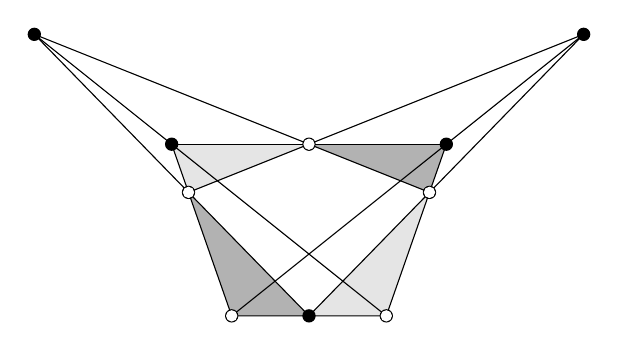
\begin{tikzpicture}[scale=0.918, x=1.9cm, y=1.9cm]

		\coordinate (A) at (0,0);
		\coordinate (B) at (1,0);
		\coordinate (C) at (2,0.8);
		\coordinate (D) at (0,-1.25);
		
		\coordinate (C') at
			([xscale=-1] {C});
		\coordinate (B') at
			([xscale=-1] {B});

		\coordinate (E) at
			(intersection of C--D and C'--A);
		\coordinate (F) at
			(intersection of B--E and D--{[xshift=1] D});
			
		\coordinate (E') at
			([xscale=-1] {E});
		\coordinate (F') at
			([xscale=-1] {F});
			
		\fill [white!70!black]
			(A) -- (B) -- (E) -- cycle;
		\fill [white!70!black]
			(E') -- (F') -- (D) -- cycle;
		\fill [white!90!black]
			(E') -- (B') -- (A) -- cycle;
		\fill [white!90!black]
			(D) -- (F) -- (E) -- cycle;

		\begin{scope}[line width=0.4pt]

		\draw (C)--(F');
		\draw (C')--(F);
		\draw (B')--(B);
		\draw (F')--(F);
		\draw (C)--(D);
		\draw (C')--(D);
		\draw (C)--(E');
		\draw (C')--(E);
		\draw (B)--(F);
		\draw (B')--(F');
		
		\end{scope}
			
		\filldraw[black] (A) circle (2.4pt);
		\filldraw[white] (A) circle (2.0pt);
		\filldraw[black] (B) circle (2.4pt);
		\filldraw[black] (B') circle (2.4pt);
		\filldraw[black] (C) circle (2.4pt);
		\filldraw[black] (C') circle (2.4pt);
		\filldraw[black] (D) circle (2.4pt);
		\filldraw[black] (E) circle (2.4pt);
		\filldraw[white] (E) circle (2.0pt);
		\filldraw[black] (E') circle (2.4pt);
		\filldraw[white] (E') circle (2.0pt);
		\filldraw[black] (F) circle (2.4pt);
		\filldraw[white] (F) circle (2.0pt);
		\filldraw[black] (F') circle (2.4pt);
		\filldraw[white] (F') circle (2.0pt);
			
	\end{tikzpicture}\hspace{0.25cm}
	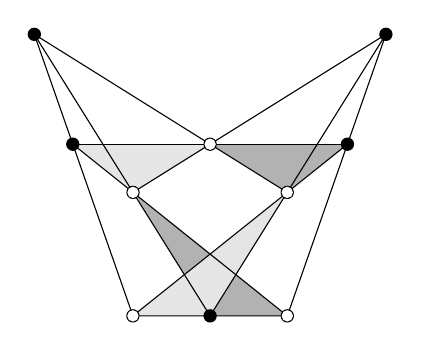
\begin{tikzpicture}[scale=0.918, x=1.9cm, y=1.9cm]
	
		\coordinate (A) at (0,0);
		\coordinate (B) at (1,0);
		\coordinate (C) at (1.28,0.8);
		\coordinate (D) at (0,-1.25);
		
		\coordinate (C') at
			([xscale=-1] {C});
		\coordinate (B') at
			([xscale=-1] {B});

		\coordinate (E) at
			(intersection of C--D and C'--A);
		\coordinate (F) at
			(intersection of B--E and D--{[xshift=1] D});
			
		\coordinate (E') at
			([xscale=-1] {E});
		\coordinate (F') at
			([xscale=-1] {F});
			
		\fill [white!70!black]
			(A) -- (B) -- (E) -- cycle;
		\fill [white!70!black]
			(E') -- (F') -- (D) -- cycle;
		\fill [white!90!black]
			(E') -- (B') -- (A) -- cycle;
		\fill [white!90!black]
			(D) -- (F) -- (E) -- cycle;
			
		\begin{scope}[line width=0.4pt]

		\draw (C)--(F');
		\draw (C')--(F);
		\draw (B')--(B);
		\draw (F')--(F);
		\draw (C)--(D);
		\draw (C')--(D);
		\draw (C)--(E');
		\draw (C')--(E);
		\draw (B)--(F);
		\draw (B')--(F');
		
		\end{scope}
			
		\filldraw[black] (A) circle (2.4pt);
		\filldraw[white] (A) circle (2.0pt);
		\filldraw[black] (B) circle (2.4pt);
		\filldraw[black] (B') circle (2.4pt);
		\filldraw[black] (C) circle (2.4pt);
		\filldraw[black] (C') circle (2.4pt);
		\filldraw[black] (D) circle (2.4pt);
		\filldraw[black] (E) circle (2.4pt);
		\filldraw[white] (E) circle (2.0pt);
		\filldraw[black] (E') circle (2.4pt);
		\filldraw[white] (E') circle (2.0pt);
		\filldraw[black] (F) circle (2.4pt);
		\filldraw[white] (F) circle (2.0pt);
		\filldraw[black] (F') circle (2.4pt);
		\filldraw[white] (F') circle (2.0pt);
			
	\end{tikzpicture}
    \caption{Конфигурация Дезарга --- пятиугольники}
    \label{fig:des}
\end{figure}

\begin{figure}[ht]
    \centering
%    \captionsetup{labelsep=colon}
	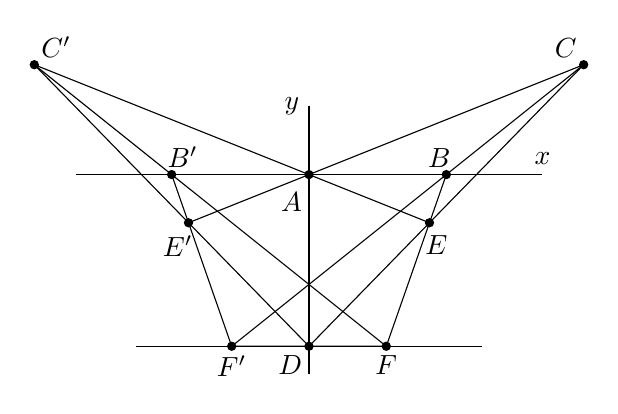
\begin{tikzpicture}[scale=0.918, x=1.9cm, y=1.9cm]
	
		\coordinate (A) at (0,0);
		\coordinate (B) at (1,0);
		\coordinate (C) at (2,0.8);
		\coordinate (D) at (0,-1.25);
		
		\coordinate (C') at
			([xscale=-1] {C});
		\coordinate (B') at
			([xscale=-1] {B});

		\coordinate (E) at
			(intersection of C--D and C'--A);
		\coordinate (F) at
			(intersection of B--E and D--{[xshift=1] D});
			
		\coordinate (E') at
			([xscale=-1] {E});
		\coordinate (F') at
			([xscale=-1] {F});
			
		\begin{scope}[line width=0.4pt]

		\draw (C)--(F');
		\draw (C')--(F);
		\draw (B')--(B);
		\draw (F')--(F);
		\draw (C)--(D);
		\draw (C')--(D);
		\draw (C)--(E');
		\draw (C')--(E);
		\draw (B)--(F);
		\draw (B')--(F');
		
		\draw (-1.7,0)--(1.7,0);
		\draw (-1.2625,-1.25)--(1.2625,-1.25);
		\draw (0,0.5)--(0,-1.45);
			
		\end{scope}
		
		\filldraw[black, opacity=0] (C) circle (2.4pt);
		\filldraw[black, opacity=0] (C') circle (2.4pt);
			
		\filldraw [black] (A) circle (1.6pt)
			node[
				yshift=-3pt,
				xshift=1pt,
				below left,
				] {\(A\)};
		\filldraw[black] (B) circle (1.6pt)
			node[
				xshift=5pt,
				yshift=-1pt,
				above left,
				] at (B) {\(B\)};
		\filldraw[black] (B') circle (1.6pt)
			node[
				xshift=-5pt,
				yshift=-1pt,
				above right,
				] at (B') {\(B'\)};
		\filldraw[black] (C) circle (1.6pt)
			node[
				xshift=1pt,
				yshift=-1pt,
				above left,
				] at (C) {\(C\)};
		\filldraw[black] (C') circle (1.6pt)
			node[
				xshift=-1pt,
				yshift=-1pt,
				above right,
				] at (C') {\(C'\)};
		\filldraw[black] (D) circle (1.6pt)
			node[
				xshift=1pt,
				below left,
				] at (D) {\(D\)};
		\filldraw[black] (E) circle (1.6pt)
			node[
				xshift=-5pt,
				yshift=-1pt,
				below right,
				] at (E) {\(E\)};
		\filldraw[black] (E') circle (1.6pt)
			node[
				xshift=5pt,
				yshift=-1pt,
				below left,
				] at (E') {\(E'\)};
		\filldraw[black] (F) circle (1.6pt)
			node[below] at (F) {\(F\)};
		\filldraw[black] (F') circle (1.6pt)
			node[below] at (F') {\(F'\)};
			
		\node [above] at (1.7,0) {\(x\)};
		\node [left] at (0,0.5) {\(y\)};
			
	\end{tikzpicture}\hspace{0.25cm}
	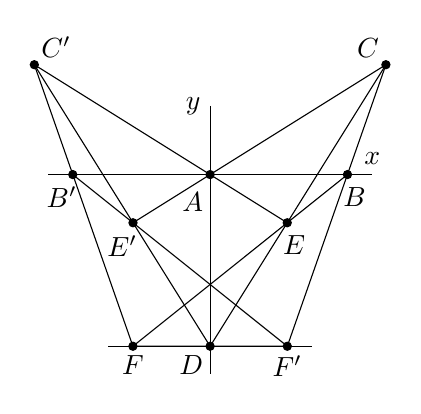
\begin{tikzpicture}[scale=0.918, x=1.9cm, y=1.9cm]
	
		\coordinate (A) at (0,0);
		\coordinate (B) at (1,0);
		\coordinate (C) at (1.28,0.8);
		\coordinate (D) at (0,-1.25);
		
		\coordinate (C') at
			([xscale=-1] {C});
		\coordinate (B') at
			([xscale=-1] {B});

		\coordinate (E) at
			(intersection of C--D and C'--A);
		\coordinate (F) at
			(intersection of B--E and D--{[xshift=1] D});
			
		\coordinate (E') at
			([xscale=-1] {E});
		\coordinate (F') at
			([xscale=-1] {F});
			
		\begin{scope}[line width=0.4pt]

		\draw (C)--(F');
		\draw (C')--(F);
		\draw (B')--(B);
		\draw (F')--(F);
		\draw (C)--(D);
		\draw (C')--(D);
		\draw (C)--(E');
		\draw (C')--(E);
		\draw (B)--(F);
		\draw (B')--(F');
		
		\draw (-1.18,0)--(1.18,0);
		\draw (-0.7425,-1.25)--(0.7425,-1.25);
		\draw (0,0.5)--(0,-1.45);
			
		\end{scope}

		\filldraw[black, opacity=0] (C) circle (2.4pt);
		\filldraw[black, opacity=0] (C') circle (2.4pt);

		\filldraw [black] (A) circle (1.6pt)
			node[
				yshift=-3pt,
				xshift=1pt,
				below left,
				] {\(A\)};
		\filldraw[black] (B) circle (1.6pt)
			node[
				xshift=-5pt,
				yshift=-1pt,
				below right,
				] at (B) {\(B\)};
		\filldraw[black] (B') circle (1.6pt)
			node[
				xshift=5pt,
				yshift=-1pt,
				below left,
				] at (B') {\(B'\)};
		\filldraw[black] (C) circle (1.6pt)
			node[
				xshift=1pt,
				yshift=-1pt,
				above left,
				] at (C) {\(C\)};
		\filldraw[black] (C') circle (1.6pt)
			node[
				xshift=-1pt,
				yshift=-1pt,
				above right,
				] at (C') {\(C'\)};
		\filldraw[black] (D) circle (1.6pt)
			node[
				xshift=1pt,
				below left,
				] at (D) {\(D\)};
		\filldraw[black] (E) circle (1.6pt)
			node[
				xshift=-5pt,
				yshift=-1pt,
				below right,
				] at (E) {\(E\)};
		\filldraw[black] (E') circle (1.6pt)
			node[
				xshift=5pt,
				yshift=-1pt,
				below left,
				] at (E') {\(E'\)};
		\filldraw[black] (F) circle (1.6pt)
			node[below] at (F) {\(F\)};
		\filldraw[black] (F') circle (1.6pt)
			node[below] at (F') {\(F'\)};
			
		\node [above] at (1.18,0) {\(x\)};
		\node [left] at (0,0.5) {\(y\)};
			
	\end{tikzpicture}
    \caption{Конфигурация Дезарга --- чертежи}
    \label{fig:des_ult}
\end{figure}

%\lettrine[lines=2]{\color{black}Н}а
\noindent
На
рисунке~\ref{fig:des} изображена конфигурация Дезарга, на которой выделены два взаимно вписанных пятиугольника. Посмотрим, как такую картинку можно нарисовать.
Применив растяжения вдоль осей \(x\) и \(y\) (рис. \ref{fig:des_ult}), можно считать, что точки \(A\), \(B\) и \(D\) фиксированы. Тогда выбор точки \(C\) задаёт рисунок: проводятся линии \(CD\), \(C'D\), \(CA\) (до \(E'\)), \(C'A\) (до \(E\)), \(CB\) (до \(F'\)), \(C'B'\) (до \(F\)). Точки \(B\), \(E\) и \(F\) всегда лежат на одной линии, что можно проверить, например, координатным методом.


\section{Элемент Казимира}

%Возьмём представление алгебры Ли: $L \to \text{End}(V)$.
%Оно индуцирует билинейную форму на $L$ --- след произведения.
%Если она невырожденная, то мы получаем следующую диаграмму:
%$$
%\text{End}_{\textit{lin}}(L)
%\longleftrightarrow
%L \otimes L^*
%\longleftrightarrow
%L \otimes L
%\longrightarrow
%\text{End}(V).
%$$
%Первая стрелка --- стандартное отождествление,
%вторая стрелка задаётся билинейной формой
%$L^* \longleftrightarrow L$, а третья стрелка
%индуцируется представлением.
%
%Для $x \in \text{End}_{\textit{lin}}(L)$ его след как элемента
%$\text{End}_{\textit{lin}}(L)$ и след его образа в $\text{End}(V)$
%совпадают (это абстрактная тавтология: след в
%$\text{End}_{\textit{lin}}(L)$ задаётся спариванием в $L \otimes L^*$
%\ldots). Берём $\text{Id}_L$ и отправляем в $\text{End}(V)$.
%Все стрелки совместимы с действием $L$, поэтому образ $\text{Id}_L$
%тоже будет $L$-инвариантен. Его след равен размерности $L$. Этот образ
%и называется {\em элементом Казимира}.

\begin{definition}[\scshape Элемент Казимира представления]
Пусть \(K\) --- поле, \(L\) --- конечномерная алгебра Ли над \(K\), а \(\rho : L \to \End_{K\module}(V)\), где \(V\) --- конечномерный \(K\)\=/модуль, --- представление \(L\), такое что билинейная форма
\(b : L \otimes_K L \to K\), \(x \otimes y \mapsto \tr(\rho(x)\rho(y))\)
невырождена.%
\label{def:CasimirElementRep}
Тогда определена следующая диаграмма:
\begin{equation}
\End_{K\module}(L)
\xlongleftarrow[\sim]{\alpha}
L \otimes_K L^{\vee}
\xlongleftarrow[\sim]{\beta}
L \otimes_K L
\xlongrightarrow{\gamma}
\End_{K\module}(V),%
\label{eq:CasimirElementDef}
\end{equation}
где \(\alpha\) --- стандартное отождествление,
изоморфизм \(\beta\) индуцирован изоморфизмом \(x \mapsto b(x,-) : L \xrightarrow{\sim} L^{\vee}\),
а отображение \(\gamma\) переводит \(x \otimes y\) в \(\rho(x)\rho(y)\) для любых \(x, y \in L\).
Элемент \(\Omega_{\rho} \coloneqq \gamma(\beta^{-1}(\alpha^{-1}(\Id_L)))\) называется \emph{элементом Казимира} представления \(\rho\).
\end{definition}

\begin{observation}[\scshape Инвариантность элемента Казимира]
В обозначениях определения~\ref{def:CasimirElementRep}
%каждая стрелка в диаграмме~\ref{eq:CasimirElementDef} --- является гомоморфизмом \(L\)\=/модулей,
отображения \(\alpha\), \(\beta\) и \(\gamma\)
являются гомоморфизмами \(L\)\=/модулей,
а потому, так как элемент \(\Id_L \in \End_{K\module}(L)\) является \(L\)\=/инвариантным, то элемент Казимира \(\Omega_{\rho}\) тоже является \(L\)\=/инвариантным.
\end{observation}

\begin{observation}[\scshape След элемента Казимира]
В обозначениях определения~\ref{def:CasimirElementRep} след любого элемента \(\End_{K\module}(L)\) совпадает со следом его образа в \(\End_{K\module}(V)\).
Это абстрактная тавтология --- надо воспользоваться тем, что след элемента \(\End_{K\module}(L)\) задаётся спариванием в \(L \otimes_K L^{\vee}\).
В частности, \(\tr(\Omega_{\rho}) = \dim_K(L)\).
\end{observation}


\section{Целые в квадратичных полях}

\begin{theorem}
Пусть \(d \in \mathbb{Z}\) --- бесквадратное целое число, а
\(
\mathcal{O}_{\mathbb{Q}[\sqrt{d}]} \coloneqq \{a+b\sqrt{d} \in \mathbb{Q}[\sqrt{d}] \mid a,b \in \Q,\ 2a \in \mathbb{Z},\ a^2-{b^2}d \in \mathbb{Z} \}
\).
Тогда если \(d \equiv 2,3 \pmod{4}\), то \(\mathcal{O}_{\mathbb{Q}[\sqrt{d}]} = \mathbb{Z}[\sqrt{d}]\), а если \(d \equiv 1 \pmod{4}\), то \(\mathcal{O}_{\mathbb{Q}[\sqrt{d}]} = \mathbb{Z}[\frac{1+\sqrt{d}}{2}]\).
\end{theorem}

\begin{proof}
Пусть \(a, b \in \mathbb{Q}\) --- числа, такие что \(2a, a^2-{b^2}d \in \mathbb{Z}\).
Так как \(a^2-{b^2}d \in \mathbb{Z}\), то \(4a^2-4{b^2}d \in \mathbb{Z}\), откуда, так как \(2a \in \mathbb{Z}\), следует, что \(4{b^2}d \in \mathbb{Z}\), откуда следует, что \(2b \in \mathbb{Z}\), так как \(d\) бесквадратное.
Осталось рассмотреть условие \(4(a^2-{b^2}d) = (2a)^2 - (2b)^2 d \equiv 0 \pmod{4}\).
\end{proof}


\section{Обратный Мура\namedash{}Пенроуза}

Пусть \(V\) и \(U\) --- абелевы группы, а \(x : V \rlarrow U : y\) --- гомоморфизмы, такие что \(xyx=x\) и \(yxy=y\).
Тогда \(yxyx=yx\) и \(xyxy=xy\), то есть \(xy\) и \(yx\) --- идемпотенты.
При этом, так как \(xyx=x\), то \(\Ker(yx) \subset \Ker(x)\), а потому \(\Ker(yx) = \Ker(x)\).
Аналогично, \(\Image(yx) = \Image(y)\), и всё то же с одновременной заменой \(x\) на \(y\) и \(y\) на \(x\).
Отсюда получаем разложения \(V = \Ker(x) \oplus \Image(y)\) и \(U = \Ker(y) \oplus \Image(x)\),
вместе с парой взаимно обратных изоморфизмов
\(v \mapsto x(v) : \Image(y) \rlarrow \Image(x) : y(u) \mapsfrom u\).

Если \(V\) и \(U\) --- это векторные пространства над \(\R\) или \(\C\) с невырожденными скалярными произведениями, то \(x\) однозначно определяет \(y\), для которого описанные разложения ортогональны. Такой \(y\) называется <<обратным Мура\namedash{}Пенроуза>> к линейному преобразованию \(x\).


\section{Теорема Эйленберга\namedash{}Уоттса}

%\begin{convention}
%Пусть \(R\text{-}\mathrm{Ab}\) ---
%категория (левых) \(R\)-мо\-ду\-лей,
%\(R\text{-}\mathrm{Ab}\text{-}S\) ---
%\((R,S)\)-би\-мо\-ду\-лей,
%\(\op{Fun}_{rng}(\mathcal{A},\mathcal{B})\) ---
%функторов \(\mathcal{A} \to \mathcal{B}\) кольцоидов.
%\end{convention}

%\begin{convention}
%Категория левых \(R\)-мо\-ду\-лей
%обозначается \(R\text{-}\mathrm{Ab}\),
%\((R,S)\)-би\-мо\-ду\-лей ---
%\(R\text{-}\mathrm{Ab}\text{-}S\),
%функторов \(\mathcal{A} \to \mathcal{B}\) кольцоидов ---
%\(\op{Fun}_{rng}(\mathcal{A},\mathcal{B})\).
%\end{convention}

%\begin{observation}
%\label{obs:colim_iso}
%Пусть \(E,E' : \mathcal{C} \to \mathcal{E}\) --- пара функторов, сохраняющих копредел функтора \(H : I \to \mathcal{C}\), а \(\omega = (\omega(C))_{C \in \Ob(\mathcal{C})} : E \Rightarrow E'\) --- естественное преобразование.
%Тогда если для каждого \(i \in \Ob(I)\) морфизм \((\omega H)(i) = \omega(H(i))\) является изоморфизмом, то \(\omega(\colim(H))\) --- тоже.
%\end{observation}

\begin{observation}[\scshape (Ко)ядро как (ко)предел]
Пусть \(f : U \to V\) --- морфизм в аддитивной категории.
Тогда \(\Coker(f)\) по определению отождествляется с \(0 \sqcup_U^f V\), а \(\Ker(f)\) --- с \(0 \times_V^f U\), где \(0\) --- нулевой объект.
\end{observation}

%\begin{theorem}[\scshape Теорема Эйленберга-Уоттса]
%Пусть \(R\) и \(S\) --- ассоциативные унитальные кольца.
%Тогда между функторами
%\[
%\begin{tikzcd}[column sep = small, cramped]
%\tensor[_S]{M}{_R}
%\mapsto
%\tensor[_S]{M}{_R} \otimes_R (-)
%:
%S\text{-}\mathrm{Ab}\text{-}R
%	\arrow[shift left]{r}{} &
%\op{Fun}_{rng} (R\text{-}\mathrm{Ab}, S\text{-}\mathrm{Ab})
%:
%\tensor[_S]{F}{}(\tensor[_R]{R}{_R})
%\mapsfrom
%F,
%	\arrow[shift left]{l}{}
%\end{tikzcd}
%\]
%где правое действие \(R\) на \(F(R)\) по функториальности индуцировано правым действием \(R\) на себе,
%существует сопряжение, заданное единицей \(\eta\) --- изоморфизмом унитальности --- и коединицей \(\varepsilon\):
%\[
%\eta(M) :
%\tensor[_S]{M}{_R}
%\xrightarrow{\sim}
%\tensor[_S]{M}{_R} \otimes_R \tensor[_R]{R}{_R},
%\quad
%(\varepsilon(F))(V) :
%\tensor[_S]{F}{}(\tensor[_R]{R}{_R})
%\otimes_R
%\tensor[_R]{V}{}
%\to
%\tensor[_S]{F}{}(\tensor[_R]{V}{}),
%\]
%где \(\varepsilon\) по \(\otimes\)-\(\Hom\) сопряжению индуцировано композицией изоморфизма унитальности и действия \(F\) на \(\Hom\)-ах:
%\[
%\tensor[_R]{V}{}
%\xrightarrow{\sim}
%\tensor[_R]{{\Hom_R}}{}(\tensor[_R]{R}{_R}, \tensor[_R]{V}{})
%\xrightarrow{f \smapsto F(f)}
%\tensor[_R]{{\Hom_S}}{}(\tensor[_S]{F}{}(\tensor[_R]{R}{_R}), \tensor[_S]{F}{}(\tensor[_R]{V}{})).
%\]
%Если функтор \(F\) сохраняет малые прямые суммы и сохраняет коядра, то есть сохраняет малые копределы, то
%\(\varepsilon(F)\) --- это изоморфизм.
%\end{theorem}

\begin{theorem}[\scshape Теорема Эйленберга\namedash{}Уоттса]
Пусть \(R\) и \(S\) --- ассоциативные унитальные кольца,
\(\mc{M}(S,R) \coloneqq (S \otimes_{\Z} R^o)\module\),
а \(\mc{F}(S,R) \coloneqq \op{Fun}_{\mr{Rngd}}(R\module, S\module)\).
Тогда определена сопряжённая пара
\begin{gather*}
%\begin{tikzcd}[
%	ampersand replacement=\&,
%	column sep = small,
%	nodes={inner xsep=1ex},
%%	nodes={inner ysep=0ex},
%	cramped,
%	]
%\tensor[_S]{M}{_R}
%\mapsto
%\tensor[_S]{M}{_R} \otimes_R (-)
%:
%S\text{-}\mathrm{Ab}\text{-}R
%	\arrow[shift left]{r}{} \&
%\op{Fun}_{rng} (R\text{-}\mathrm{Ab}, S\text{-}\mathrm{Ab})
%:
%\tensor[_S]{F}{}(\tensor[_R]{R}{_R})
%\mapsfrom
%F,
%	\arrow[shift left]{l}{}
%\end{tikzcd}
\tensor[_S]{M}{_R}
\mapsto
\tensor[_S]{M}{_R} \otimes_R (-)
:
\mc{M}(S,R) \rlarrow \mc{F}(S,R)
:
\tensor[_S]{F}{}(\tensor[_R]{R}{_R})
\mapsfrom
F,
\\
\eta(M) :
\tensor[_S]{M}{_R}
\xrightarrow{\sim}
\tensor[_S]{M}{_R} \otimes_R \tensor[_R]{R}{_R},
\;
(\varepsilon(F))(V) :
\tensor[_S]{F}{}(\tensor[_R]{R}{_R})
\otimes_R
\tensor[_R]{V}{}
\to
\tensor[_S]{F}{}(\tensor[_R]{V}{}),
\end{gather*}
где правое действие \(R\) на \(F(R)\) по функториальности индуцировано правым действием \(R\) на себе, единица \(\eta\) --- это изоморфизм унитальности, а коединица \(\varepsilon\) по \(\otimes\)-\(\Hom\) сопряжению индуцирована композицией изоморфизма унитальности и действия \(F\) на \(\Hom\)-ах:
\[
\tensor[_R]{V}{}
\xrightarrow{\sim}
\tensor[_R]{{\Hom_R}}{}(\tensor[_R]{R}{_R}, \tensor[_R]{V}{})
\xrightarrow{f \mapsto F(f)}
\tensor[_R]{{\Hom_S}}{}(\tensor[_S]{F}{}(\tensor[_R]{R}{_R}), \tensor[_S]{F}{}(\tensor[_R]{V}{})).
\]
Если функтор \(F\) сохраняет малые прямые суммы и сохраняет коядра, то есть сохраняет малые копределы, то
\(\varepsilon(F)\) --- это изоморфизм.
\end{theorem}

\begin{proofparts}[Доказательство (из трёх частей)]

\item[Часть 1.]
Заметим, что гомоморфизм \((\varepsilon(F))(R) : F(R) \otimes_R R \to F(R)\) --- это просто изоморфизм унитальности.

\item[Часть 2.]
Если функтор \(F\) сохраняет малые прямые суммы, то из части~1 этого доказательства следует, что \(\varepsilon(F)\) является изоморфизмом и для малых прямых сумм копий \(R\), то есть для свободных модулей.

\item[Часть 3.]
Если функтор \(F\) сохраняет ещё и коядра, то из части~2 этого доказательства следует, что \(\varepsilon(F)\) является изоморфизмом и для коядер гомоморфизмов свободных модулей, то есть для всех модулей.
\qedhere

\end{proofparts}



\chapter{Подкорректированные старые тексты}


\section{Теорема Гамильтона\namedash{}Кэли}

\subsection{Формулировка и доказательство}

%\begin{theorem}[\scshape Теорема Гамильтона-Кэли]
%Пусть \(\varphi \in \End_{A\tn{-}\mr{mod}}(A^I)\), где \(I\) --- конечное множество, а \(A\) --- ассоциативное коммутативное унитальное кольцо.
%\label{thm:Cayley-Hamilton}
%Тогда \(\varphi\) является корнем своего характеристического многочлена.
%\end{theorem}
%
%\begin{proof}
%%Эндоморфизм \(\varphi\) превращает \(V \coloneqq A^I\) в \(A[X]\)-мо\-дуль, а \(V^I\) --- в \(\Mat_I (A[X])\)-мо\-дуль.
%Эндоморфизм \(\varphi\) индуцирует на \(V \coloneqq A^I\) структуру \(A[X]\)-мо\-ду\-ля, которая индуцирует на \(V^I\) структуру \(\Mat_I (A[X])\)-мо\-ду\-ля.
%Пусть \((e_i)_{i \in I}\) --- стандартный \(A\)-базис \(V\), рассмотренный как элемент \(V^I\),
%а
%\(
%s \coloneqq
%(X \delta_{i,j} - a_{i,j})_{i,j \in I}
%=
%X - (a_{i,j})_{i,j \in I}
%\in \Mat_I (A[X])
%\),
%где \((a_{i,j})_{i,j \in I}\) --- матрица \(\varphi\) в базисе \((e_i)_{i \in I}\),
%а \(\delta_{i,j}\) --- дельта Кронекера.
%Тогда
%\(s \cdot (e_i)_{i \in I} = 0\).
%Умножив это равенство слева на присоединённую матрицу к \(s\), получаем, что
%\(\det(s) \cdot (e_i)_{i \in I} = (\det(s) \cdot e_i)_{i \in I} = 0\),
%то есть
%многочлен
%\(\det(s) \in A[X]\)
%зануляет \(A\)-ба\-зис \(V\),
%а потому и всё \(V\),
%%его образ \(\det(s) \in A[X]\) в \(\End_{A\tn{-}\mr{mod}}(V)\) равен нулю,
%что и требовалось доказать.
%\end{proof}

\begin{theorem}[\scshape Теорема Гамильтона\namedash{}Кэли]
Если \(x\) --- эндоморфизм свободного конечно порождённого модуля \(V\) над ассоциативным коммутативным унитальным кольцом \(A\),%
\label{thm:Cayley-Hamilton}
то \(x\) является корнем своего характеристического многочлена.
\end{theorem}

\begin{proof}%[Набросок доказательства]
Эндоморфизм
\(
\varphi \mapsto \varphi x :
\End_{A\module}(V) \to \End_{A\module}(V)
\)
превращает \(\End_{A\module}(V)\)\=/модуль \(\End_{A\module}(V)\) в модуль над кольцом \(\End_{A\module}(V)[X] \cong \End_{A\module}(V) \otimes_A A[X] \cong \End_{A[X]\module}(V \otimes_A A[X])\),
при этом \(\Id_V\) зануляется элементом \(c \coloneqq x - X\), а потому и элементом \(\op{adj}(c) c = \det(c) \in A[X] \subset \End_{A[X]\module}(V \otimes_A A[X])\).
\end{proof}

\begin{remark}
Приведённое доказательство теоремы Гамильтона\namedash{}Кэли изложено в статье Алексея Муранова~\cite{Muranov_2022}.
\end{remark}

\begin{observation}
Пусть \(A\) --- ассоциативное коммутативное унитальное кольцо, \(V\) --- конечно порождённый \(A\)\=/модуль, а \(\varphi \in \End_{A\module}(V)\).
По определению \(V\) существует сюръективный гомоморфизм \(\pi : A^I \to V\), где \(I\) --- какое-то конечное множество.
%Для любого такого \(\pi\)
По проективности \(A^I\)
существует эндоморфизм \(\widetilde{\varphi} \in \End_{A\module}(A^I)\), такой что \(\varphi \circ \pi = \pi \circ \widetilde{\varphi}\),
называемый поднятием \(\varphi\).
Для любого такого \(\widetilde{\varphi}\) любой многочлен из \(A[X]\), зануляющий \(\widetilde{\varphi}\), например, характеристический многочлен \(\widetilde{\varphi}\), зануляет и \(\varphi\).
\end{observation}

\subsection{Дополнение}

\begin{theorem} 
Пусть \(\varphi \in \End_{A\module}(A^n)\), где \(n \in \N_0\), а \(A\) --- ассоциативное коммутативное унитальное кольцо.
Тогда характеристический многочлен \(\varphi\) равен \(\sum_{i=0}^n (-1)^i \tr(\bigwedge^i \varphi) X^{n-i} \in A[X]\).
%Тогда \(c_i = (-1)^i \tr(\bigwedge^i \varphi)\), где \(1 \leq i \leq n\).
\end{theorem}

\begin{proof}[Идея доказательства]
Двойной счёт по множеству пар, состоящих из перестановки \(n\)-элементного множества и подмножества в множестве её фиксированных точек.
\end{proof}

\begin{observation}
Пусть \(B \coloneqq A[X]/(P(X))\), где \(A\) --- ассоциативное коммутативное унитальное кольцо, а \(P(X) \in A[X]\) --- унитальный многочлен. Пусть \(x \in B\) --- это образ \(X \in A[X]\).
Очевидно, что множество \(\{x^i \in B \mid 0 \leq i < \deg(P(X))\}\) является \(A\)-базисом \(B\).
Идеал многочленов в \(A[X]\), зануляющих оператор
\(x : B \to B\), \(f \mapsto xf\),
равен \((P(X))\), как сразу видно прямо из определения \(B\).
В частности, характеристический многочлен \(x\) равен \(P(X)\).
\end{observation}

\begin{observation}
Присоединённую матрицу к матрице \((x_{i,j})_{i,j \in I}\) можно определить формулой
\(
%\op{adj}((x_{i,j})_{i,j \in I}) \coloneqq
(\sum_{\sigma \in \Aut(I) \suchthat \sigma(j) = i} \op{sgn}(\sigma) \prod_{k \in I \setminus \{j\}} x_{k,\sigma(k)})_{i,j \in I}
\).
\end{observation}

\subsection{Некоторые следствия}

\begin{theorem}
Пусть \(M\) --- конечно порождённый модуль над коммутативным ассоциативным унитальным кольцом \(A\),
а \(\iota\) --- ненулевой инъективный эндоморфизм \(M\).%
\label{thm:FinGenModOverCommRingInj}
%Тогда существует \(a \in A \setminus \{0\}\), такой что \(aM \subset \iota(M)\).
Тогда \(\Ann_A(\Coker(\iota)) \neq 0\).
\end{theorem}

\begin{proof}
Из теоремы Гамильтона\namedash{}Кэли следует, что существует унитальный многочлен \(P(X) = \sum_{i=0}^n a_i X^i \in A[X]\) минимальной степени \(n \in \N_1\),
такой что \(P(\iota) = 0\).
%Воспользовавшись тем, что на \(\iota\) можно сокращать слева, легко заметить, что \(a_0 \neq 0\).
Так как на \(\iota\) можно сокращать слева, то \(a_0 \neq 0\).
%Возьмём \(a \coloneqq -a_0\).
Тогда \(a_0 v = -\sum_{i=1}^n a_i \iota^i(v) \in \iota(M)\) для любого \(v \in M\), то есть \(a_0 \in \Ann_A(\Coker(\iota))\).
\end{proof}

\begin{corollary}
Пусть \(A\) --- ненулевое коммутативное ассоциативное унитальное кольцо, а \(n, m \in \N_1\) --- числа, такие что \(n > m\). Тогда не существует инъективного гомоморфизма \(A\)\=/модулей \(\iota : A^n \to A^m\).
\end{corollary}

\begin{proof}
Пусть \(\iota' : A^m \to A^n\) --- какое-то координатное вложение. Тогда \(\iota' \circ \iota\) --- ненулевой инъективный эндоморфизм \(A^n\),
%образ которого не содержит \(aA^n\) ни для какого \(a \in A \setminus \{0\}\),
%такой что \(aA^n \not\subset (\iota' \circ \iota)(A^n)\) для любого \(a \in A \setminus \{0\}\),
такой что \(\Ann_A(\Coker(\iota' \circ \iota)) = 0\),
что противоречит теореме~\ref{thm:FinGenModOverCommRingInj}.
\end{proof}

%\begin{remark}
%Известно, что любой сюръективный эндоморфизм конечно порождённого модуля над коммутативным ассоциативным унитальным кольцом является изоморфизмом.
%\end{remark}


\section{Тензорное произведение}

\subsection{Тензорное произведение абелевых групп}

\begin{notation}
В этом разделе \(\Hom\) без индексов обозначает \(\Hom\) как абелевых групп. То же верно насчёт \(\otimes\) и \(\End\).
\end{notation}

\begin{definition}[\scshape Тензорное произведение] \label{def:AbTensorProd}
Определим \emph{тензорное произведение} конечного семейства абелевых групп \((V_i)_{i \in I}\) как абелеву группу \(\bigotimes_{i \in I} V_i\),
заданную образующими --- формальными произведениями \(\bigotimes_{i \in I} v_i\),
биективными семействам \((v_i)_{i \in I} \in \prod_{i \in I} V_i\),
%--- и соотношениями дистрибутивности ---
--- и соотношениями ---
\(
\textstyle
(v' + v'')_{\otimes e} \otimes (\bigotimes_{i \in I \setminus \{e\}} v_i) =
v'_{\otimes e} \otimes (\bigotimes_{i \in I \setminus \{e\}} v_i) +
v''_{\otimes e} \otimes (\bigotimes_{i \in I \setminus \{e\}} v_i),
\)
где \(e \in I\),
\(v', v'' \in V_e\),
\(v_i \in V_i\) для любого \(i \in I \setminus \{e\}\).
\end{definition}

\begin{remark}
Индекс \(\otimes e\) в выражении \(v'_{\otimes e}\), называемый \emph{позиционным индексом}, указывает на место \(v'\) в формальном произведении. 
%Вот ещё один пример использования позиционных индексов:
%\(V^{\otimes I} = \bigotimes_{i \in I} V_{\otimes i}\).
Группировка тензорных мономов считается ясной из контекста.
\end{remark}

\begin{observation}
Пусть \((V_i)_{i \in I}\) --- пустое семейство абелевых групп, то есть \(I = \varnothing\).
Тогда \(\bigotimes_{i \in I} V_i \cong \Z\).
\end{observation}

\begin{observation}
Пусть \((V_i)_{i \in I}\) --- конечное семейство абелевых групп, а \(\bigotimes_{i \in I} v_i \in \bigotimes_{i \in I} V_i\). Тогда если \(v_e = 0\) для какого-то \(e \in I\), то \(\bigotimes_{i \in I} v_i = 0\).
\end{observation}

\begin{definition}[\scshape Функториальность \(\otimes\)]
Пусть \((\varphi_i : V_i \to U_i)_{i \in I}\) --- конечное семейство гомоморфизмов абелевых групп.
Тогда гомоморфизм
\(\bigotimes_{i \in I} \varphi_i :
\bigotimes_{i \in I} V_i \to
\bigotimes_{i \in I} U_i\),
\(\bigotimes_{i \in I} v_i
\mapsto
\bigotimes_{i \in I} \varphi_i(v_i)\)
называется \emph{тензорным произведением} семейства \((\varphi_i)_{i \in I}\).
\end{definition}

\begin{statement}[\scshape Сопряжённость \(\otimes\) и \(\Hom\)]
Пусть \(V\), \(U\) и \(M\) --- абелевы группы.
Тогда имеем следующий естественный изоморфизм:
\begin{equation}\label{eq:TensorHomAdj}
\begin{tikzcd}[column sep = 8.5em]
\Hom(M \otimes V, U)
	\arrow[shift left]{r}{\varphi \mapsto (v \mapsto (m \mapsto \varphi(m \otimes v)))} &
\Hom(V, \Hom(M, U)).
	\arrow[shift left]{l}{((\psi(v))(m) \mapsfrom m \otimes v) \mapsfrom \psi}
\end{tikzcd}
\end{equation}
\end{statement}

\begin{statement}[\scshape Унитальность \(\otimes\)]
Пусть \(V\) --- абелева группа.
Тогда имеем естественный изоморфизм
\(
a \otimes v \mapsto av :
\Z \otimes V \rlarrow V
: 1 \otimes v \mapsfrom v
\).
\end{statement}

\begin{statement}[\scshape Дистрибутивность \(\otimes\)] \label{sta:TensorDistr}
Пусть \(\pi : I \to J\) --- отображение множеств, \(J\) конечно, \((V_i)_{i \in I}\) --- семейство абелевых групп.
Пусть \(\op{Sec}(\pi) \coloneqq \{\sigma : J \to I \mid \pi \circ \sigma = \mathrm{Id}_J\}\).
Тогда проекции на слагаемые и вложения слагаемых прямых сумм индуцируют пару взаимно обратных гомоморфизмов:
\(
\bigotimes_{j \in J}
	\bigoplus_{i \in \pi^{-1}(j)}
		V_i
\rlarrow
\bigoplus_{\sigma \in \op{Sec}(\pi)}
	\bigotimes_{j \in J}
		V_{\sigma(j)}
\).
\end{statement}

\begin{statement}[\scshape Точность справа \(\otimes\)] \label{sta:TensorRightExact}
Пусть \(I\) --- конечное множество, \((V_i)_{i \in I}\) и \((U_i)_{i \in I}\) --- семейства абелевых групп, причём \(U_i\) является подгруппой \(V_i\) для любого \(i \in I\).
Тогда следующая последовательность с очевидным образом определёнными гомоморфизмами точна:
\[
\textstyle
\bigoplus_{e \in I} ((U_e)_{\otimes e} \otimes (\bigotimes_{i \in I \setminus \{e\}} V_i))
\to
\bigotimes_{i \in I} V_i
\to
\bigotimes_{i \in I} (V_i / U_i)
\to
0.
\]
\end{statement}

\begin{proof}
Пусть \(\mathcal{U} \subset \bigotimes_{i \in I} V_i\) --- это образ первого гомоморфизма.
Тогда обратный к гомоморфизму
\((\bigotimes_{i \in I} V_i) / \mathcal{U} \to \bigotimes_{i \in I} (V_i / U_i)\)
определяется на образующих так:
\(
\bigotimes_{i \in I} (v_i + U_i)
\mapsto
(\bigotimes_{i \in I} v_i) + \mathcal{U}
\).
Определение корректно --- образ
\(\bigotimes_{i \in I} (v_i + U_i)\) зависит только от классов \(v_i + U_i \in V_i/U_i\), где \(i \in I\).
\end{proof}

\begin{example}
Пусть \(R\) --- кольцо, а \(\mf{I} \subset R\) --- аддитивная подгруппа, такая что \(R\mf{I} + \mf{I}R \subset \mf{I}\), то есть двусторонний идеал. Тогда отображение умножения \(R \otimes R \to R\) индуцирует отображение \((R/\mf{I}) \otimes (R/\mf{I}) \cong (R \otimes R) / (R \otimes \mf{I} + \mf{I} \otimes R) \to R/\mf{I}\).
\end{example}

%\begin{lemma}[\scshape Бинарная ассоциативность \(\otimes\)]
%Пусть \(I = I_1 \sqcup I_2\) --- конечное множество,
%\((V_i)_{i \in I}\) --- семейство абелевых групп.
%Тогда следующий гомоморфизм является изоморфизмом:
%\[
%\textstyle
%\bigotimes_{i \in I} V_i
%	\xrightarrow{\sim}
%(\bigotimes_{i \in I_1} V_i)
%\otimes
%(\bigotimes_{i \in I_2} V_i),
%\quad
%\bigotimes_{i \in I} v_i
%\mapsto
%(\bigotimes_{i \in I_1} v_i)
%\otimes
%(\bigotimes_{i \in I_2} v_i).
%\]
%\end{lemma}
%
%\begin{proof}
%Обратный гомоморфизм задаётся по сопряжению:
%\[
%\textstyle
%\bigotimes_{i \in I_1} V_i
%\to
%\Hom(\bigotimes_{i \in I_2} V_i, \bigotimes_{i \in I} V_i),
%\
%\bigotimes_{i \in I_1} v_i
%\mapsto
%(\bigotimes_{i \in I_2} v_i \mapsto \bigotimes_{i \in I} v_i).
%\qedhere
%\]
%\end{proof}

\begin{statement}[\scshape Ассоциативность \(\otimes\)]
Пусть \(\pi : I \to J\) --- отображение конечных множеств, \((V_i)_{i \in I}\) --- семейство абелевых групп.
\label{sta:TensorAbAss}
Тогда имеем следующий изоморфизм:
\begin{equation}\label{eq:TensorAssIso}
\textstyle
\bigotimes_{i \in I} V_i
\leftrightarrow
\bigotimes_{j \in J}
	\bigotimes_{i \in \pi^{-1}(j)} V_i,
\quad
\bigotimes_{i \in I} v_i
\leftrightarrow
\bigotimes_{j \in J}
	\bigotimes_{i \in \pi^{-1}(j)} v_i.
\end{equation}
\end{statement}

\begin{proof}[Набросок доказательства]
Согласно определению~\ref{def:AbTensorProd} представим каждый из \(\bigotimes_{i \in \pi^{-1}(j)} V_i\) как фактор свободной абелевой группы, порождённой формальными тензорными мономами, после чего воспользуемся точностью справа \(\bigotimes_{j \in J}(-)\) в смысле утверждения~\ref{sta:TensorRightExact}, ну и дистрибутивностью \(\bigotimes\) относительно \(\bigoplus\), то есть утверждением~\ref{sta:TensorDistr}.
\end{proof}

%\begin{proof}
%Докажем индукцией по мощности \(J\). Если мощность \(J\) строго больше двух, представим \(J\) в виде \(J = J_1 \sqcup J_2\), где \(J_1,J_2 \neq \varnothing\). Пусть \(I_1 \coloneqq \pi^{-1}(J_1)\), \(I_2 \coloneqq \pi^{-1}(J_2)\). По индукции получаем цепочку изоморфизмов:
%\(
%\bigotimes_{i \in I} V_i
%\leftrightarrow
%(\bigotimes_{i \in I_1} V_i)
%\otimes
%(\bigotimes_{i \in I_2} V_i)
%\leftrightarrow
%(\bigotimes_{j \in J_1} \bigotimes_{i \in \pi^{-1}(j)} V_i)
%\otimes
%(\bigotimes_{j \in J_2} \bigotimes_{i \in \pi^{-1}(j)} V_i)
%\leftrightarrow
%\bigotimes_{j \in J} \bigotimes_{i \in \pi^{-1}(j)} V_i
%\).
%\end{proof}

\begin{definition}[\scshape Тензорное произведение колец]
Пусть \((R_i)_{i \in I}\) --- конечное семейство колец.
Определим на абелевой группе \(\bigotimes_{i \in I} R_i\) умножение следующим образом:
\begin{gather*}
\textstyle
(\bigotimes_{i \in I} R_i)
\otimes
(\bigotimes_{i \in I} R_i)
\xrightarrow{\sim}
\bigotimes_{i \in I} (R_i \otimes R_i)
\to
\bigotimes_{i \in I} R_i,
\\
\textstyle
(\bigotimes_{i \in I} r'_i)
\otimes
(\bigotimes_{i \in I} r''_i)
\mapsto
\bigotimes_{i \in I} (r'_i \otimes r''_i)
\mapsto
\bigotimes_{i \in I} (r'_i r''_i).
\end{gather*}
Первое отображение --- это изоморфизм ассоциативности, а второе --- это тензорное произведение отображений умножения в индивидуальных кольцах.
\end{definition}

\begin{statement}[\scshape Универсальное свойство тензорного произведения колец]
Пусть \((R_i)_{i \in I}\) --- конечное семейство ассоциативных унитальных колец.
Тогда кольцо \(\bigotimes_{i \in I} R_i\) снабжено семейством гомоморфизмов
\(\iota_e : R_e \to \bigotimes_{i \in I} R_i\),
\(r \mapsto r_{\otimes e} \otimes \bigotimes_{i \in I \setminus \{e\}} 1_{\otimes i}\), где \(e \in I\),
причём образы \(\iota_e\) и \(\iota_{e'}\) при \(e \neq e'\) поэлементно коммутируют.
Пусть \(S\) --- ассоциативное унитальное кольцо, а \((\epsilon_e : R_e \to S)_{e \in I}\) --- семейство гомоморфизмов, такое что образы \(\epsilon_e\) и \(\epsilon_{e'}\) при \(e \neq e'\) поэлементно коммутируют.
Тогда существует единственный гомоморфизм \(\varphi : \bigotimes_{i \in I} R_i \to S\), такой что \(\varphi \circ \iota_e = \epsilon_e\) для любого \(e \in I\).
\end{statement}

\subsection{Тензорное произведение с коэффициентами}

\subsubsection{Бинарное тензорное произведение с коэффициентами}

\begin{definition}%
%[\scshape Нулевые (ко)гомологии Хохшильда]
[\scshape (Ко)инварианты Хохшильда]
Пусть \(M\) --- бимодуль над ассоциативным унитальным кольцом \(R\). Определим его
%\emph{нулевые гомологии и когомологии Хохшильда}
\emph{инварианты и коинварианты Хохшильда}
следующим образом:
\begin{align*}
\sop{HH}^0(R, M) &\coloneqq M^{\mf{h}(R)} =
\{m \in M \mid rm = mr\ \text{для всех}\ r \in R\},\\
\sop{HH}_0(R, M) &\coloneqq \mathrlap{M_{\mf{h}(R)}}\phantom{M^{\mf{h}(R)}} =
M / (rm = mr \mid r \in R,\ m \in M),
%M / (\Z\{rm - mr \mid r \in R,\ m \in M\}),
\end{align*}
где
факторизация в определении \(\sop{HH}_0(R, M)\) --- это факторизация абелевой группы по соотношениям, а
\(\mf{h}(R)\) --- это кольцо Ли ассоциативного кольца \(R\), действующее на абелевой группе \(M\)
%с помощью гомоморфизма
через композицию гомоморфизма
\(r \mapsto r \otimes 1 - 1 \otimes r : \mf{h}(R) \to R \otimes R^o\)
со структурным гомоморфизмом \(R \otimes R^o \to \End(M)\).
\end{definition}

\begin{example}
Пусть \(R\) --- ассоциативное унитальное кольцо, \(V = \tensor[_R]{V}{}\) и \(U = \tensor[_R]{U}{}\) --- левые \(R\)-мо\-ду\-ли.
Тогда
%\(\Hom_R(V, U) \cong \sop{HH}^0(R, \Hom(V, U))\).
\(\Hom_R(\tensor[_R]{V}{}, \tensor[_R]{U}{}) \cong (\Hom(V, U))^{\mf{h}(R)}\).
\end{example}

\begin{definition}[\scshape Бинарное тензорное произведение с коэффициентами]
Пусть \(R\) --- ассоциативное унитальное кольцо, \(V = \tensor[]{V}{_R}\) --- правый \(R\)-модуль, \(U = \tensor[_R]{U}{}\) --- левый \(R\)-модуль.
Определим \emph{тензорное произведение} \(V\) и \(U\) над \(R\) следующим образом:
%\(
%V \otimes_R U
%\coloneqq
%\sop{HH}_0(R, V \otimes U)
%\).
\(
\tensor[]{V}{_R} \otimes_R \tensor[_R]{U}{}
\coloneqq
(V \otimes U)_{\mf{h}(R)}
\).
\end{definition}

%\begin{observation}
%Пусть \(S\), \(R\) и \(T\) --- ассоциативные унитальные кольца, \(M = \tensor[_S]{M}{_R}\) --- \(S\)-\(R\)-би\-мо\-дуль, \(V = \tensor[_R]{V}{}\) --- левый \(R\)-мо\-дуль, \(U = \tensor[_S]{U}{}\) --- левый \(S\)-мо\-дуль.
%Тогда естественная биекция \eqref{eq:TensorHomAdj}
%индуцирует естественную биекцию
%\(
%\Hom_{S} (\tensor[_S]{M}{_R} \otimes_R \tensor[_R]{V}{}, \tensor[_S]{U}{})
%\rlarrow
%\Hom_{R} (\tensor[_R]{V}{}, \Hom_{S} (\tensor[_S]{M}{_R}, \tensor[_S]{U}{}))
%\):
%\begin{align*}
%& \mathrel{\phantom{\cong}} \sop{HH}^0(S,
%	\Hom(\sop{HH}_0(R, M \otimes V), U))
%\cong
%\\
%& \cong \sop{HH}^0(S,
%	\sop{HH}^0(R, \Hom(M \otimes V, U)))
%\cong
%\\
%& \cong \sop{HH}^0(R,
%	\sop{HH}^0(S, \Hom(V, \Hom(M, U))))
%\cong
%\\
%& \cong \sop{HH}^0(R,
%	\Hom(V, \sop{HH}^0(S, \Hom(M, U)))).
%\end{align*}
%\end{observation}

\begin{observation}
Пусть \(S\), \(R\) и \(T\) --- ассоциативные унитальные кольца, \(M = \tensor[_S]{M}{_R}\) --- \(S\)-\(R\)-би\-мо\-дуль, \(V = \tensor[_R]{V}{}\) --- левый \(R\)-мо\-дуль, \(U = \tensor[_S]{U}{}\) --- левый \(S\)-мо\-дуль.
Тогда изоморфизм \eqref{eq:TensorHomAdj}
индуцирует изоморфизм
%\begin{gather*}
%\Hom_{S} (\tensor[_S]{M}{_R} \otimes_R \tensor[_R]{V}{}, \tensor[_S]{U}{})
%\cong
%\sop{HH}^0(S, \Hom(\sop{HH}_0(R, M \otimes V), U))
%\cong
%\\
%\cong
%\sop{HH}^0(S, \sop{HH}^0(R, \Hom(M \otimes V, U)))
%\cong
%\\
%\cong
%\sop{HH}^0(R, \sop{HH}^0(S, \Hom(V, \Hom(M, U))))
%\cong
%\\
%\cong
%\sop{HH}^0(R, \Hom(V, \sop{HH}^0(S, \Hom(M, U))))
%\cong
%\Hom_{R} (\tensor[_R]{V}{}, \Hom_{S} (\tensor[_S]{M}{_R}, \tensor[_S]{U}{})).
%\end{gather*}
\begin{gather*}
\Hom_{S} (\tensor[_S]{M}{_R} \otimes_R \tensor[_R]{V}{}, \tensor[_S]{U}{})
\cong
(\Hom((M \otimes V)_{\mf{h}(R)}, U))^{\mf{h}(S)}
\cong
\\
\cong
((\Hom(M \otimes V, U))^{\mf{h}(R)})^{\mf{h}(S)}
\cong
((\Hom(V, \Hom(M, U)))^{\mf{h}(S)})^{\mf{h}(R)}
\cong
\\
\cong
(\Hom(V, (\Hom(M, U))^{\mf{h}(S)}))^{\mf{h}(R)}
\cong
\Hom_{R} (\tensor[_R]{V}{}, \Hom_{S} (\tensor[_S]{M}{_R}, \tensor[_S]{U}{})).
\end{gather*}
\end{observation}

\begin{observation}[\scshape Функторы замены кольца]
Пусть \(S \to R\) --- гомоморфизм ассоциативных унитальных колец.
Такой гомоморфизм индуцирует функтор \emph{ограничения скаляров}: \(\op{res}^R_S : R\text{-}\mathrm{Mod} \to S\text{-}\mathrm{Mod}\), наделяющий \(R\)-модуль \(\tensor[_R]{V}{}\) структурой \(S\)-модуля с помощью сквозного гомоморфизма \(S \to R \to \End(V)\),
а также индуцирует на \(R = \tensor[_R]{R}{_S} = \tensor[_S]{R}{_R}\) структуры \(R\)-\(S\)-би\-мо\-ду\-ля и \(S\)-\(R\)-би\-мо\-ду\-ля.
Естественные изоморфизмы унитальности
\(\Hom_R(\tensor[_R]{R}{_S}, \tensor[_R]{V}{}) \leftrightarrow \op{res}^R_S(\tensor[_R]{V}{}) \leftrightarrow \tensor[_S]{R}{_R} \otimes_R \tensor[_R]{V}{}\)
переводят изоморфизмы сопряжённости между \(\otimes\) и \(\Hom\) в изоморфизмы следующих сопряжённостей:
\(
\tensor[_R]{R}{_S} \otimes_S (-)
\dashv
\op{res}^R_S(-)
\dashv
\Hom_S(\tensor[_S]{R}{_R}, -)
\).
Функтор \(\tensor[_R]{R}{_S} \otimes_S (-)\) называется \emph{расширением скаляров},
\(\Hom_S(\tensor[_S]{R}{_R}, -)\) --- \emph{корасширением скаляров},
а все три вместе --- \emph{функторами замены кольца}.
\end{observation}

%\begin{remark}
%Никто не мешает взять
%%ванильное тензорное произведение \(\bigotimes_{i \in I} V_i\)
%тензорное произведение семейства абелевых групп
%и рассмотреть нулевые гомологии Хохшильда сразу по нескольким коммутирующим действиям колец. Читателю предлагается при желании сформулировать соответствующие определения и доказать нужные утверждения самостоятельно, благо они следуют из уже доказанных результатов про тензорные произведения абелевых групп.
%\end{remark}

\subsubsection{Тензорное произведение с коэффициентами для семейств}

%\begin{definition}[\scshape Система коэффициентов]
%Пусть \(I\) --- конечное множество.
%\label{def:TensorSysCoeff}
%Пусть \((R_{i,i'})_{(i,i') \in I^{\times 2} \setminus \Delta}\) --- семейство ассоциативных унитальных колец, такое что для любых \(i \neq i'\) кольца \(R_{i,i'}\) и \(R_{i',i}\) противоположны, то есть \(R_{i,i'} = R_{i',i}^o\).
%Такие семейства колец будем называть \emph{системами коэффициентов}.
%%Пусть \((V_i)_{i \in I}\) --- семейство абелевых групп.
%Мы будем говорить, что система коэффициентов \((R_{i,i'})_{(i,i') \in I^{\times 2} \setminus \Delta}\) действует на семействе абелевых групп \((V_i)_{i \in I}\), если для каждого \(i' \in I\) абелева группа \(V_{i'}\) снабжена поэлементно коммутирующими действиями колец \(R_{i,i'}\), где \(i \in I \setminus \{i'\}\).
%\end{definition}

\begin{definition}[\scshape Система коэффициентов]
Пусть \(I\) --- конечное множество.
\label{def:TensorSysCoeff}
Тогда будем называть \emph{системой коэффициентов} семейство ассоциативных унитальных колец \((R_{i,i'})_{(i,i') \in I^{\times 2} \setminus \Delta}\), такое что \(R_{i,i'} = R_{i',i}^o\) для всех \((i,i') \in I^{\times 2} \setminus \Delta\).
\end{definition}

\begin{definition}[\scshape Действие системы коэффициентов]
\label{def:TensorSysCoeffAct}
Будем говорить, что на конечном семействе абелевых групп \((V_i)_{i \in I}\) действует система коэффициентов \((R_{i,i'})_{(i,i') \in I^{\times 2} \setminus \Delta}\), если для каждого \(i' \in I\) абелева группа \(V_{i'}\) снабжена
структурой модуля над \(\bigotimes_{i \in I \setminus \{i'\}} R_{i,i'}\).
%поэлементно коммутирующими действиями колец \(R_{i,i'}\), где \(i \in I \setminus \{i'\}\).
\end{definition}

\begin{definition}[\scshape Тензорное произведение с коэффициентами]
%Пусть \(I\) --- конечное множество.
Пусть система коэффициентов \((R_{i,i'})_{(i,i') \in I^{\times 2} \setminus \Delta}\) действует на конечном семействе абелевых групп \((V_i)_{i \in I}\).
\label{def:TensorGenProdCoeff}
%Пусть \((R_{i,j})_{(i,j) \in I^{\times 2} \setminus \Delta}\) --- семейство ассоциативных унитальных колец, такое что \(R_{i,j} = R_{j,i}^o\) для любых \((i,j) \in I^{\times 2} \setminus \Delta\),
%а \((V_i)_{i \in I}\) --- семейство абелевых групп,
%причём для каждого \(j \in I\) абелева группа \(V_j\) снабжена коммутирующими действиями колец \(R_{i,j}\), где \(i \in I \setminus \{j\}\).
Тогда
\emph{тензорное произведение} семейства \((V_i)_{i \in I}\) над \((R_{i,i'})_{(i,i') \in I^{\times 2} \setminus \Delta}\),
обозначаемое
\(\bigotimes^{R_{i,i'}}_{i \in I} V_i\),
--- это фактор абелевой группы \(\bigotimes_{i \in I} V_i\) по соотношениям типа
\[
\textstyle
(v_i r_{i,i'})_{\otimes i} \otimes (\bigotimes_{k \in I \setminus \{i\}} v_k)
=
(r_{i,i'} v_{i'})_{\otimes i'} \otimes (\bigotimes_{k \in I \setminus \{i'\}} v_k),
\]
где \((i,i') \in I^{\times 2} \setminus \Delta\),
\(r_{i,i'} \in R_{i,i'}\),
\((v_k)_{k \in I} \in \prod_{k \in I} V_k\).
\end{definition}

\begin{statement}[\scshape Ассоциативность]
Пусть \(\pi : I \to J\) --- отображение конечных множеств. Пусть на семействе абелевых групп \((V_i)_{i \in I}\) действует система коэффициентов \((R_{i,i'})_{(i,i') \in I^{\times 2} \setminus \Delta}\).
\label{sta:TensorCoeffAss}
Тогда изоморфизм ассоциативности \eqref{eq:TensorAssIso}
%\(
%%\textstyle
%\bigotimes_{i \in I} V_i
%\leftrightarrow
%\bigotimes_{j \in J}
%	\bigotimes_{i \in \pi^{-1}(j)} V_i
%\)
индуцирует изоморфизм фактор\-/групп
\[
\textstyle
\bigotimes^{R_{i,i'}}_{i \in I} V_i
\leftrightarrow
\bigotimes^{\mathcal{R}_{j,j'}}_{j \in J}
	\bigotimes^{R_{i,i'}}_{i \in \pi^{-1}(j)} V_i,\
\tn{где}\
\mathcal{R}_{j,j'} \coloneqq
\bigotimes_{(i,i') \in \pi^{-1}(j) \times \pi^{-1}(j')} R_{i,i'}.
\]
\end{statement}

\begin{proof}[Набросок доказательства]
Утверждение~\ref{sta:TensorCoeffAss} можно получить из утверждения~\ref{sta:TensorAbAss} с помощью утверждения~\ref{sta:TensorRightExact}.
\end{proof}

\begin{remark}
Определения~\ref{def:TensorSysCoeff}, \ref{def:TensorSysCoeffAct}, \ref{def:TensorGenProdCoeff} и утверждение~\ref{sta:TensorCoeffAss} добавлены с иллюстративными целями, чтобы показать, что определение тензорного произведения не зависит от порядка на множестве индексов.
\end{remark}


\section{Коммутативная локализация}

\subsection{Определение и задание локализации}

\begin{convention}
В этом разделе категория моноидов под заданным моноидом называется категорией моноидов над заданным моноидом.
\end{convention}

%\begin{definition}[\scshape Локализация моноида]
%Пусть дано отображение множества \(S\) в мультипликативный моноид \(T\). Определим \emph{локализацию} \(T\) по \(S\), обозначаемую \(S^{-1}T\), как начальный объект в категории моноидов под \(T\), в которых образы элементов \(S\) обратимы.
%\end{definition}

%\begin{definition}[\scshape Локализация кольца]
%%Пусть \(R\) --- это ассоциативное унитальное кольцо, а \(S \to R\) --- отображение множеств.
%Пусть дано отображение множества \(S\) в ассоциативное унитальное кольцо \(R\).
%Определим \emph{локализацию} \(R\) по \(S\), обозначаемую \(S^{-1}R\), как начальный объект в категории ассоциативных унитальных колец над \(R\), в которых образы элементов \(S\) мультипликативно обратимы.
%\end{definition}

\begin{definition}[\scshape Локализация моноида или кольца]
Пусть дано отображение множества \(S\) в мультипликативный моноид или ассоциативное унитальное кольцо \(R\).
Определим \emph{локализацию} \(R\) по \(S\), обозначаемую \(S^{-1}R\), как начальный объект в категории моноидов над \(R\) или ассоциативных унитальных колец над \(R\) соответственно, в которых образы элементов \(S\) мультипликативно обратимы.
%Определим \emph{локализацию} \(R\) по \(S\), обозначаемую \(S^{-1}R\),
%как моноид или ассоциативное унитальное кольцо соответственно, полученный
%добавлением к \(R\) семейства переменных \((X_s)_{s \in S}\) и факторизацией по семейству соотношений
%\((X_s s = s X_s = 1)_{s \in S}\).
\end{definition}

\begin{observation}[\scshape Задание локализации]
Пусть дано отображение множества \(S\) в мультипликативный моноид или ассоциативное унитальное кольцо \(R\).
Тогда соответствующая локализация \(S^{-1}R\) может быть задана добавлением к \(R\) семейства переменных \((X_s)_{s \in S}\) и факторизацией по семейству соотношений
\((X_s s = s X_s = 1)_{s \in S}\).
\end{observation}

%\begin{remark}
%Локализация моноида или кольца по множеству обладает очевидным универсальным свойством.
%\end{remark}

%\begin{observation}[\scshape Задание локализации моноида или кольца]
%Ясно, что локализация моноида \(T\) по множеству \(S \subset T\) может быть задана
%добавлением к \(T\) семейства переменных \((X_s)_{s \in S}\) и факторизацией по семейству соотношений
%\((X_s s = s X_s = 1)_{s \in S}\).
%То же верно для локализации ассоциативного унитального кольца.
%\end{observation}

%\begin{observation}[\scshape Задание локализации кольца]
%Ясно, что локализация ассоциативного унитального кольца \(R\) по множеству \(S \subset R\) может быть задана
%добавлением к \(R\) семейства переменных \((X_s)_{s \in S}\) и факторизацией по семейству соотношений
%\((X_s s = s X_s = 1)_{s \in S}\).
%\end{observation}

%\begin{observation}[\scshape Локализация моноида с нулём]
%Пусть \(M\) --- мультипликативный моноид с нулём, а \(S \subset M\) --- его подмоноид.
%Тогда образ нуля из \(M\) в \(S^{-1}M\) является нулём в \(S^{-1}M\).
%\end{observation}

\begin{definition}[\scshape Мультипликативное множество]
Подмоноид в мультипликативном моноиде иногда называется \emph{мультипликативным мно\-жес\-твом}.
\end{definition}

\begin{observation}
%Очевидно, что локализация по множеству совпадает с локализацией по его образу в моноиде, которая совпадает с локализацией по мультипликативному моноиду, порождённому образом.
Очевидно, что локализация мультипликативного моноида или ассоциативного унитального кольца \(R\) по множеству \(S\) совпадает с локализацией \(R\) по свободному моноиду, порождённому \(S\),
и совпадает с локализацией \(R\) по образу \(S\) в \(R\).
%и, если \(M\) коммутативен, совпадает с локализацией \(M\) по сатурации образа \(S\) в \(M\).
\end{observation}

%\begin{definition}[\scshape \(R\)\=/Объект]
%Пусть \(\mc{C}\) и \(\mc{R}\) --- две категории или два кольцоида, такие что \(\Ob(\mc{R}) = \pt\),
%а \(R \coloneqq \Ar(\mc{R})\).
%Тогда объект \(X \in \Ob(\mc{C})\), снабжённый гомоморфизмом \(R \to \End_{\mc{C}}(X)\), то есть действием \(R\), называется \emph{\(R\)\=/объектом}.
%Категория \(R\)\=/объектов в \(\mc{C}\) обозначается \(\mc{C}^{\mc{R}}\).
%\end{definition}

\begin{definition}[\scshape \(R\)\=/Объект]
Пусть \(\mc{C}\) --- категория или кольцоид, а \(R\) --- моноид или ассоциативное унитальное кольцо соответственно.
Тогда объект \(X \in \Ob(\mc{C})\), снабжённый действием \(R\), то есть гомоморфизмом \(R \to \End_{\mc{C}}(X)\), называется \emph{\(R\)\=/объектом}.
Категория \(R\)\=/объектов в \(\mc{C}\) обозначается \(\mc{C}^{\mc{R}}\), где \(\mc{R}\) --- это \(R\) как однообъектная категория/кольцоид.
\end{definition}

%\begin{definition}[\scshape Локализация объекта с действием моноида]
%Пусть \(\mc{C}\) --- категория, \(R\) --- моноид, \(X\) --- \(R\)\=/объект в \(\mc{C}\), а \(S\) --- множество, снабжённое отображением \(S \to R\).%
%\label{def:LocObjMonAct}
%Определим \emph{локализацию} \(X\) по \(S\), обозначаемую \(S^{-1}X\), как начальный объект в категории \(R\)\=/объектов \(Y\) под \(X\), таких что \(s : Y \to Y\) является изоморфизмом для любого \(s \in S\).
%\end{definition}

%\begin{remark}
%Локализация объекта с действием ассоциативного унитального кольца определяется совершенно аналогично определению~\ref{def:LocObjMonAct}.
%\end{remark}

%\begin{remark}
%В обозначениях определения~\ref{def:LocObjMonAct} локализация \(R\)\=/объекта по \(S\) --- это расширение скаляров вдоль \(R \to S^{-1}R\).
%\end{remark}

%\begin{definition}[\scshape Локализация объекта с действием]
%Пусть \(\mc{C}\) и \(\mc{R}\) --- две категории или два кольцоида, причём \(\mc{R}\) однообъектная,
%\(S\) --- множество, снабжённое отображением в \(R \coloneqq \Ar(\mc{R})\),
%а \(X\) --- \(R\)\=/объект в \(\mc{C}\).%
%\label{def:LocObjMonAct}
%Тогда \emph{локализация} \(X\) по \(S\), обозначаемая \(S^{-1}X\), ---
%это расширение скаляров вдоль канонического гомоморфизма \(R \to S^{-1}R\) для \(X\).
%\end{definition}

\begin{definition}[\scshape Локализация объекта с действием]
Пусть \(\mc{C}\) --- категория или кольцоид, \(R\) --- моноид или ассоциативное унитальное кольцо соответственно, \(X\) --- \(R\)\=/объект в \(\mc{C}\), а \(S\) --- множество, снабжённое отображением \(S \to R\).%
\label{def:LocObjMonAct}
Определим \emph{локализацию} \(X\) по \(S\)
%обозначаемую \(S^{-1}X\),
как расширение скаляров вдоль канонического гомоморфизма \(R \to S^{-1}R\) для \(X\).
%как начальный объект в категории \(R\)\=/объектов \(Y\) под \(X\), таких что \(s : Y \to Y\) является изоморфизмом для любого \(s \in S\).
\end{definition}

\begin{notation}%[\scshape Обозначения локализации]
Локализация объекта \(X\) по \(S\) обычно обозначается через \(S^{-1}X\), \(X_S\) или \(X[S^{-1}]\).
Если \(S = A \setminus \mf{p}\)
--- теоретико-множественное дополнение простого идеала \(\mf{p}\) в ассоциативном коммутативном унитальном  кольце \(A\),
а \(M\) --- \(A\)\=/модуль,
то вместо \(M_S\) часто пишут \(M_{\mf{p}}\).
\end{notation}

%\begin{definition}[\scshape Локализация множества с действием моноида]
%Пусть \(T\) --- моноид, \(S \subset T\) --- мультипликативное множество, а \(X\) --- \(T\)\=/множество.
%Определим \emph{локализацию} \(X\) по \(S\), обозначаемую \(S^{-1}X\), как начальный объект в категории \(T\)\=/множеств \(Y\) под \(X\), таких что для любого \(s \in S\) отображение \(y \mapsto sy : Y \to Y\) биективно.
%\end{definition}

%\begin{definition}[\scshape Локализация модуля]
%Пусть \(M\) --- модуль над ассоциативным унитальным кольцом \(R\), а \(S \subset R\) --- мультипликативное множество.
%Определим \emph{локализацию} \(M\) по \(S\), обозначаемую \(S^{-1}M\), как начальный объект в категории \(R\)\=/модулей \(N\) под \(M\), таких что для любого \(s \in S\) отображение \(v \mapsto sv : N \to N\) биективно.
%\end{definition}

%\begin{definition}
%Пусть \(S\) --- моноид, \(X\) --- \(S^o\)\=/множество, а \(Y\) --- \(S\)\=/множество.
%Тогда
%\(X \circledast_S Y \coloneqq (X \times Y) / ((xs,y) \sim (x,sy))_{s \in S, x \in X, y \in Y}\).
%Класс \([(x, y)] \in X \circledast_S Y\), где \(x \in X\) и \(y \in Y\), будет обозначаться через \(x \circledast y\).
%\end{definition}

%\begin{observation}
%Пусть \(S \to D\) --- гомоморфизм моноидов, а \(X\) --- \(S\)\=/множество.
%Тогда на множестве \(D \circledast_S X\) определена структура \(D\)\=/множества: \(d'(d \circledast x) = (d'd) \circledast x\), где \(d,d' \in D\), а \(x \in X\), и определён гомоморфизм \(S\)\=/множеств \(x \mapsto 1 \circledast x : X \to D \circledast_S X\), вместе с которым \(D \circledast_S X\) становится начальным объектом в категории \(D\)\=/множеств под \(X\).
%\end{observation}

%\begin{observation}
%Пусть \(T\) --- моноид, \(S \subset T\) --- мультипликативное множество, а \(X\) --- \(T\)\=/множество.%
%\label{obs:LocMonAndLocSet}
%Тогда \(T\)\=/множество
%%\[X_S \coloneqq ((S^{-1}T) \times X) / ((ws, x) \sim (w, sx) \mid w \in S^{-1}T,\ s \in S,\ x \in X)\]
%\(X_S \coloneqq (S^{-1}T) \circledast_S X\)
%%где \(a[(w,x)] \coloneqq [(aw,x)]\) для любых \(a \in T\), \(w \in S^{-1}T\) и \(x \in X\), снабжённое гомоморфизмом \(x \mapsto [(1,x)] : X \to X_S\),
%%удовлетворяет универсальному свойству \(S^{-1}X\).
%является локализацией \(T\)\=/множества \(X\) по \(S\).
%\end{observation}

%\begin{observation}
%Пусть \(M\) --- модуль над ассоциативным унитальным кольцом \(R\), а \(S \subset R\) --- мультипликативное множество.%
%\label{obs:LocRingAndLocMod}
%Тогда \(R\)\=/модуль \((S^{-1}R) \otimes_R M\)
%%удовлетворяет универсальному свойству \(S^{-1}M\).
%является локализацией \(R\)\=/модуля \(M\) по \(S\).
%\end{observation}

%\begin{remark}
%Для действий моноидов на множествах тоже существует расширение скаляров, и локализацию множества с действием моноида по подмоноиду можно описать аналогично наблюдению~\ref{obs:LocRingAndLocMod}.
%\end{remark}

%\begin{observation}
%Пусть \(T\) --- моноид, а \(S \subset T\) --- его подмоноид.
%Тогда из наблюдения~\ref{obs:LocMonAndLocSet} сразу ясно, что локализация \(T\) по \(S\) как \(T\)\=/множества и локализация \(T\) по \(S\) как моноида канонически отождествляются.
%\end{observation}

\begin{observation}[\scshape Согласованность]
Пусть \(R\) --- моноид или ассоциативное унитальное кольцо, а \(S \subset R\) --- мультипликативное множество.
Тогда
%из наблюдения~\ref{obs:LocRingAndLocMod} сразу ясно, что
локализация \(R\) по \(S\) как \(R\)\=/множества или \(R\)\=/модуля соответственно канонически отождествляется с локализацией \(R\) по \(S\) как моноида или ассоциативного унитального кольца соответственно.
\end{observation}


\subsection{Коммутативная локализация как фильтрованный копредел}

\begin{observation}[\scshape Локализация по центральному подмножеству]
%Пусть \(\mc{C}\) --- категория или кольцоид, \(R\) --- моноид или ассоциативное унитальное кольцо соответственно, \(\mc{R}\) --- это \(R\) как однообъектная категория/кольцоид, \(X\) --- \(R\)\=/объект в \(\mc{C}\), а \(S \subset \Zent(R)\) --- центральное мультипликативное множество.
Пусть \(\mc{C}\) и \(\mc{R}\) --- две категории или два кольцоида, такие что \(\mc{R}\) однообъектна,
\(X\) --- \(R\)\=/объект в \(\mc{C}\), где \(R \coloneqq \Ar(\mc{R})\), а \(S \subset \Zent(R)\) --- центральное мультипликативное множество.
%Тогда
%морфизм \(\gamma_1\)
%%фильтрованный копредел
%из наблюдения~\ref{obs:LocFilteredColim} для \(\mc{E} \coloneqq \mc{C}^{\mc{R}}\) и \(S\)\=/объекта \(X\) является локализацией \(R\)\=/объекта \(X\) по \(S\).
Тогда локализация \(X\) по \(S\) как \(S\)\=/объекта в \(\mc{C}^{\mc{R}}\) является локализацией \(X\) по \(S\) как \(R\)\=/объекта в \(\mc{C}\).
\end{observation}

\begin{definition}[\scshape Категория Кэли моноида]
Пусть \(S\) --- моноид,
%а \(\mc{S}\) --- тот же \(S\), рассматриваемый как категория с одним объектом.
а \(\mc{S}\) --- это \(S\) как однообъектная категория.
Тогда определён функтор \(\mc{S} \to \mr{Sets}\), переводящий \(s \in \Ar(\mc{S}) = S\) в \(x \mapsto sx : S \to S\).%
\label{def:CayleyCatMon}
Категория элементов этого функтора называется \emph{категорией Кэли} моноида \(S\) и обозначается \(\mr{Cay}(S)\).
Она снабжена каноническим функтором \(\mr{Cay}(S) \to \mc{S}\).
\end{definition}

%\begin{remark}
%В обозначениях определения~\ref{def:CayleyCatMon} категория \(\mr{Cay}(S)\) снабжена каноническим функтором \(\mr{Cay}(S) \to \mc{S}\).
%\end{remark}

\begin{observation}
Для любого коммутативного моноида его категория Кэли является фильтрованной категорией.
\end{observation}

%\begin{observation}[\scshape Локализация как копредел]
%Пусть
%\(T\) --- коммутативный моноид,
%\(S \subset T\) --- подмоноид,
%\(X\) --- \(T\)\=/множество,
%\(\mc{S}\) --- это \(S\) как однообъектная категория,
%\(C : \mr{Cay}(S) \to \mc{S}\) --- канонический функтор,
%\(F : \mc{S} \to \mr{Sets}\) --- функтор, заданный индуцированным действием \(S\) на \(X\),
%а \((\gamma_s : X \to \colim(F \circ C))_{s \in S \cong \Ob(\mr{Cay}(S))}\) --- копредельный коконус \(F \circ C\).%
%\label{obs:LocFilteredColim}
%Тогда,
%так как действия \(T\) и \(S\) на \(X\) коммутируют, то
%\(T\) действует на \(F\), а потому и на \(\colim(F \circ C)\).
%Морфизм \(\gamma_1\) --- это локализация \(X\) по \(S\).
%%Тогда,
%%так как действие \(T\) на \(X\) коммутирует с действием \(S\) на \(X\), то
%%\(T\) действует на \(F\) естественными преобразованиями.
%%%Копредел композиции канонического функтора \(\mr{Cay}(S) \to S'\) и \(F\) является локализацией \(T\)\=/множества \(X\) по \(S\).
%%Соответствующая \(1 \in S \cong \Ob(\mr{Cay}(S))\) компонента копредельного коконуса функтора \(F \circ C\) является локализацией \(T\)\=/множества \(X\) по \(S\).
%%%Если \((\gamma_s : X \to X_S)_{s \in S}\) --- копредельный конус композиции канонического функтора \(\mr{Cay}(S) \to S'\) и \(F\), то \(\gamma_1\) --- это локализация \(X\) по \(S\).
%\end{observation}

%\begin{observation}[\scshape Локализация как копредел]
%Пусть
%\(R\) --- коммутативный моноид,
%\(S \subset R\) --- подмоноид,
%%\(X\) --- \(R\)\=/множество,
%\(\mc{S}\) и \(\mc{R}\) --- это \(S\) и \(R\) как однообъектные категории,
%\(P : \mr{Cay}(S) \to \mc{S}\) --- канонический функтор,
%\(\mc{C}\) --- категория,
%\(\widetilde{F} : \mc{R} \to \mc{C}\) --- действие \(R\) на \(X \in \Ob(\mc{C})\),
%а \(F \coloneqq \widetilde{F}|_{\mc{S}}\).
%Тогда если \((\gamma_s : X \to \colim(F \circ P))_{s \in S \cong \Ob(\mr{Cay}(S))}\) --- копредельный коконус \(F \circ P\),%
%\label{obs:LocFilteredColim}
%то,
%так как действия \(R\) и \(S\) на \(X\) коммутируют,
%\(R\) действует на \(F\), а потому и на \(\colim(F \circ P)\),
%и морфизм \(\gamma_1\) --- это локализация \(X\) по \(S\).
%И наоборот, если \(\gamma_1 : X \to S^{-1}X\) --- локализация,
%то семейство \((\gamma_s \coloneqq s^{-1} \circ \gamma_1 : X \to S^{-1}X)_{s \in S}\) --- это копредельный коконус \(F \circ P\).
%\end{observation}

%\begin{observation}[\scshape Локализация как копредел]
%Пусть
%\(R\) --- моноид,
%\(S \subset \Zent(R)\) --- центральный подмоноид,
%\(\mc{S}\) и \(\mc{R}\) --- это \(S\) и \(R\) как однообъектные категории,
%\(P : \mr{Cay}(S) \to \mc{S}\) --- канонический функтор,
%\(\mc{C}\) --- категория,
%\(X\) --- \(R\)\=/объект в \(\mc{C}\),
%а \(F : \mc{S} \to \mc{C}^{\mc{R}}\) --- индуцированное действие \(S\) на \(X\).
%Тогда если \((\gamma_s : X \to \colim(F \circ P))_{s \in S \cong \Ob(\mr{Cay}(S))}\) --- копредельный коконус \(F \circ P\),%
%\label{obs:LocFilteredColim}
%то морфизм \(\gamma_1\) --- это локализация \(X\) по \(S\).
%\end{observation}

\begin{observation}[\scshape Локализация как копредел]
Пусть
\(S\) --- коммутативный моноид,
\(\mc{S}\) --- это \(S\) как однообъектная категория,
\(\mc{C}\) --- категория,
\(P : \mr{Cay}(S) \to \mc{S}\) --- канонический функтор,
%\(X\) --- \(S\)\=/объект в \(\mc{C}\),
а \(F : \mc{S} \to \mc{C}\) --- функтор действия на \(S\)\=/объект \(X\).
Тогда если \((\gamma_s : X \to \colim(F \circ P))_{s \in S \cong \Ob(\mr{Cay}(S))}\) --- копредельный коконус \(F \circ P\),%
\label{obs:LocFilteredColim}
%то \(S\) действует на \(F\), а потому и на \(\colim(F \circ P)\),
то \(S\) действует на \(\colim(F \circ P)\) через действие на \(F\),
и морфизм \(\gamma_1\) --- это локализация \(X\) по \(S\).
\end{observation}

\begin{remark}
В обозначениях наблюдения~\ref{obs:LocFilteredColim} 
для любого \(r \in S\)
морфизм
\(r^{-1} : \colim(F \circ P) \to \colim(F \circ P)\)
индуцирован коконусом \((\gamma_{rs})_{s \in S}\).
\end{remark}

\begin{question}
Существуют ли категория \(\mc{C}\), коммутативный моноид \(S\) и \(S\)\=/объект \(X\) в \(\mc{C}\), такие что локализация \(X\) по \(S\) существует, но фильтрованный копредел \(\colim(F \circ P)\) из наблюдения~\ref{obs:LocFilteredColim} не существует?
\end{question}

%\begin{example}[\scshape Локализация по центральному множеству]
%%Пусть \(\mc{C}\) --- категория или кольцоид, \(R\) --- моноид или ассоциативное унитальное кольцо соответственно, \(\mc{R}\) --- это \(R\) как однообъектная категория/кольцоид, \(X\) --- \(R\)\=/объект в \(\mc{C}\), а \(S \subset \Zent(R)\) --- центральное мультипликативное множество.
%Пусть \(\mc{C}\) и \(\mc{R}\) --- две категории или два кольцоида, такие что \(\mc{R}\) однообъектна,
%\(X\) --- \(R\)\=/объект в \(\mc{C}\), где \(R \coloneqq \Ar(\mc{R})\), а \(S \subset \Zent(R)\) --- центральное мультипликативное множество.
%Тогда
%морфизм \(\gamma_1\)
%%фильтрованный копредел
%из наблюдения~\ref{obs:LocFilteredColim} для \(\mc{E} \coloneqq \mc{C}^{\mc{R}}\) и \(S\)\=/объекта \(X\) является локализацией \(R\)\=/объекта \(X\) по \(S\).
%\end{example}

%\begin{observation}[\scshape Локализация как копредел]
%Пусть
%\(R\), \(\mc{R}\), \(S\), \(\mc{S}\), \(P\), \(\mc{C}\), \(\widetilde{F}\) и \(F\) такие же, как в наблюдении~\ref{obs:LocFilteredColim}, а \(\gamma_1 : X \to S^{-1}X\) --- локализация.%
%\label{obs:FilteredColimLoc}
%Тогда \((\gamma_s \coloneqq s^{-1} \circ \gamma_1 : X \to S^{-1}X)_{s \in S}\) --- копредельный коконус \(F \circ P\).
%\end{observation}

%\begin{remark}
%Локализация действия ассоциативного унитального кольца по центральному мультипликативному множеству точно так же выражается как фильтрованный копредел по категории Кэли.
%\end{remark}

\begin{notation}[\scshape Дроби]
В обозначениях наблюдения~\ref{obs:LocFilteredColim},
если \(\mc{C} = \mr{Sets}\), то
элементами \(\colim(F \circ P)\) являются классы пар \((x, s) \in X \times S\),
рассматриваемых по модулю отношения эквивалентности, порождённого соотношениями
\((x, s) \sim (rx, rs)\), где \(r, s \in S\) и \(x \in X\),
которые мы будем обозначать через \(x/s\) или \(\frac{x}{s}\) и называть \emph{дробями}.
При этом \(a \frac{x}{s} = \frac{ax}{s}\) для всех \(a \in R\), \(s \in S\) и \(x \in X\), а \(\gamma_1 : X \to \colim(F \circ P)\), \(x \mapsto \frac{x}{1}\).
\end{notation}

%\begin{observation}
%Пусть \(S\) --- коммутативный моноид, \(X\) --- \(S\)\=/множество,
%а \(x, y \in X\) --- элементы \(X\).%
%\label{obs:CommLocSetMainAlt}
%Тогда равенство образов \(x\) и \(y\) в \(S^{-1}X\) эквивалентно существованию \(s \in S\), такого что \(sx = sy\).
%\end{observation}

\begin{observation}
Пусть \(R\) --- моноид, \(S \subset \Zent(R)\) --- центральный подмоноид, \(X\) --- \(R\)\=/множество,
а \(x\) и \(y\) --- элементы \(X\).%
\label{obs:CommLocSetMainAlt}
Тогда равенство образов \(x\) и \(y\) в \(S^{-1}X\) эквивалентно существованию \(s \in S\), такого что \(sx = sy\).
\end{observation}

%\begin{remark}
%Описание коммутативной локализации, данное в этом подподразделе, является лаконичным, но требует знакомства с элементарным категорным языком. В следующем подподразделе для удобства читателя будет дано более элементарное описание той же конструкции.
%\end{remark}

%\subsubsection{Явное описание коммутативной локализации}
%
%\begin{observation}
%%Пусть \(S\) --- коммутативный моноид, а \(X\) --- \(S\)\=/множество.%
%Пусть \(T\) --- коммутативный моноид, \(S \subset T\) --- мультипликативное множество, а \(X\) --- \(T\)\=/множество.%
%\label{obs:SetCommOpLocalMain}
%Тогда \(T\)\=/множество
%\(X_S \coloneqq (X \times S) / ((x, s) \sim (rx,rs))_{x \in X, s,r \in S}\),
%%\[M_S \coloneqq (M \times S) / ((a, s) \sim (ra,rs) \mid a \in M,\ s,r \in S),\]
%где \(a[(x, s)] \coloneqq [(ax, s)]\) для любых \(a \in T\), \(x \in X\) и \(s \in S\), снабжённое гомоморфизмом \(x \mapsto [(x,1)] : X \to X_S\),
%%удовлетворяет универсальному свойству \(S^{-1}X\).
%является локализацией \(T\)\=/множества \(X\) по \(S\).
%\end{observation}
%
%\begin{notation}
%В обозначениях наблюдения~\ref{obs:SetCommOpLocalMain} класс \([(x, s)] \in X_S\) пары \((x, s) \in X \times S\) будет обозначаться через \(x/s\) или \(\frac{x}{s}\) и называться \emph{дробью}.
%\end{notation}
%
%\begin{lemma}
%Пусть \(X\) --- множество, а \(S\) --- коммутативный моноид, действующий на \(X\) инъективными эндоморфизмами.%
%\label{lem:CommLocSetMainInj}
%Тогда канонический гомоморфизм \(X \to S^{-1}X\) инъективен.
%\end{lemma}
%
%\begin{proof}
%Введём на множестве \(X \times S\) отношение \((x_1, s_1) \sim (x_2, s_2) \iff x_1 s_2 = s_1 x_2\).
%Пусть \((x_1, s_1), (x_2, s_2), (x_3, s_3) \in X \times S\). Тогда условие \((x_1, s_1) \sim (x_2, s_2)\) эквивалентно условию \(x_1 s_2 s_3 = s_1 x_2 s_3\), условие \((x_2, s_2) \sim (x_3, s_3)\) --- условию \(s_1 x_2 s_3 = s_1 s_2 x_3\), а условие \((x_1, s_1) \sim (x_3, s_3)\) --- условию \(x_1 s_2 s_3 = s_1 s_2 x_3\), откуда ясно, что \(\sim\) --- это отношение эквивалентности.
%Сразу видно, что данное отношение эквивалентности порождено соотношениями \((x, s) \sim (rx,rs)\), где \(x \in X\), \(s,r \in S\).
%\end{proof}
%
%\begin{theorem}
%Пусть \(S\) --- коммутативный моноид, \(X\) --- \(S\)\=/множество,
%а \(x, y \in X\) --- элементы \(X\).%
%\label{thm:CommLocSetMain}
%Тогда равенство образов \(x\) и \(y\) в \(S^{-1}X\) эквивалентно существованию \(s \in S\), такого что \(sx = sy\).
%\end{theorem}
%
%\begin{proof}
%Действие моноида \(S\) на \(X\) наследуется множеством \(\overline{X} \coloneqq X / (x \sim y \mid \exists s \in S : sx = sy)\), причём элементы \(S\) действуют на \(\overline{X}\) инъекциями.
%Очевидно, что
%локализации \(X\) и \(\overline{X}\) по \(S\) канонически изоморфны.
%Осталось применить лемму~\ref{lem:CommLocSetMainInj}.
%\end{proof}
%
%%\begin{observation}
%%Пусть \(S\) --- коммутативный моноид, а \(\iota: X \to Y\) --- инъективный гомоморфизм \(S\)\=/множеств.%
%%\label{InjHomLocSets}
%%Тогда индуцированный гомоморфизм \(S^{-1}\iota : S^{-1}X \to S^{-1}Y\) инъективен.
%%\end{observation}
%
%%\begin{theorem}
%%Пусть \(T\) --- коммутативный мультипликативный моноид, а \(S \subset T\) --- его подмоноид.%
%%\label{thm:CommMonLocalMain}
%%Тогда каноническое отображение из локализации \(T\) как \(S\)\=/множества в локализацию \(T\) по \(S\) как моноида биективно.
%%\end{theorem}
%
%%\begin{proof}
%%Пусть \(S^{-1}T\) --- локализация \(T\) по \(S\) как моноида, а \(T_S\) --- локализация \(T\) как \(S\)\=/множества.
%%Тогда, по функториальности, \(T\) действует на \(T_S\), что индуцирует действие \(S^{-1}T\) на \(T_S\).
%%Соответствующее отображение \(q \mapsto q 1 : S^{-1}T \to T_S\) обратно каноническому отображению \(T_S \to S^{-1}T\).
%%\end{proof}

%\subsubsection{Сатурация, то есть насыщение, подмоноида}

\begin{definition}[\scshape Сатурация центрального подмоноида]
%Пусть \(R\) --- коммутативный мультипликативный моноид, а \(S \subset R\) --- его подмоноид.
Пусть \(R\) --- моноид, а \(S \subset \Zent(R)\) --- центральный подмоноид.
Определим \emph{насыщение} или \emph{сатурацию} \(S\) в \(R\) как
%\(
%S^\mr{sat} \coloneqq
%\{a \in R \mid \exists s \in S : a \mid s\}
%%=
%%\Bigl\{a \in A \Bigm\vert \frac{a}{1} \in (S^{-1}A)^\times\Bigr\}.
%%\{a \in M \mid a/1 \in (S^{-1}M)^\times\}
%\).
\(
S^\mr{sat} \coloneqq
\{a \in R \mid Ra \cap S \cap aR \neq \varnothing\}
\).
Множество \(S^\mr{sat}\) мультипликативно. Если \(S = S^\mr{sat}\), то \(S\) называется \emph{насыщенным} или \emph{сатурированным} мультипликативным множеством.
\end{definition}

\begin{observation}
%Пусть \(R\) --- коммутативный мультипликативный моноид, а \(S \subset R\) --- его подмоноид.
Пусть \(R\) --- моноид, а \(S \subset \Zent(R)\) --- центральный подмоноид.
Тогда \(S^\mr{sat} = \{a \in R \mid a/1 \in (S^{-1}R)^\times\}\).
\end{observation}

\subsection{Аддитивная локализация полукольца}

%\subsubsection{Определение кольца формальных разностей}

\begin{notation}[\scshape Формальные разности]
Если \(R\) --- аддитивно записываемый коммутативный моноид, а \(S \subset R\) --- его подмоноид, то элементы локализации \(R\) по \(S\), обозначаемой \(R - S\), называются \emph{формальными разностями} и записываются в виде \(a - s\), где \(a \in R\), \(s \in S\).
\end{notation}

\begin{definition}[\scshape Аддитивная локализация полукольца]
Пусть дано отображение множества \(S\) в полукольцо с нулём \(R\). Определим \emph{аддитивную локализацию} \(R\) по \(S\), обозначаемую \(R - S\), как начальный объект в категории полуколец с нулём под \(R\), в которых образы элементов \(S\) аддитивно обратимы.
\end{definition}

\begin{definition}[\scshape Двусторонний полуидеал]
Пусть \(R\) --- полукольцо с нулём.
Тогда подмножество \(S \subset R\) называется \emph{двусторонним полуидеалом}, если \(S\) является аддитивным подмоноидом \(R\) и \(RS + SR \subset R\).
\end{definition}

\begin{observation}
Ясно, что аддитивная локализация полукольца с нулём \(R\) по подмножеству \(S \subset R\) совпадает с аддитивной локализацией \(R\) по двустороннему полуидеалу в \(R\), порождённому \(S\).
\end{observation}

%\subsubsection{Явное описание кольца формальных разностей}

\begin{theorem}
Пусть \(R\) --- полукольцо с нулём, \(S \subset R\) --- двусторонний полуидеал, а \(R - S\) --- соответствующая локализация аддитивных моноидов.%
\label{thm:SemiringAddLocal}
Тогда на \(R - S\) существует единственное дистрибутивное умножение, относительно которого канонический аддитивный сохраняющий ноль гомоморфизм \(R \to R - S\) мультипликативен.
\end{theorem}

\begin{proof}[Набросок доказательства]
Произведение двух формальных разностей определяется формулой \((a_1 - s_1)(a_2 - s_2) = (a_1 a_2 + s_1 s_2) - (a_1 s_2 + s_1 a_2)\). Сразу видно, что это определение корректно.
\end{proof}

\begin{observation}
В обозначениях теоремы~\ref{thm:SemiringAddLocal}
%снабжённое каноническим гомоморфизмом \(R \to R - S\)
полукольцо с нулём \(R - S\)
является аддитивной локализацией полукольца с нулём \(R\) по \(S\).
\end{observation}

%\subsection{Локализация коммутативного кольца}

%\subsubsection{Локализация модуля над коммутативным кольцом}

%\subsubsection{Определение и задание локализации кольца}

%\subsubsection{Явное описание коммутативной локализации}

%\begin{theorem}
%Пусть \(M\) --- модуль над ассоциативным коммутативным унитальным кольцом \(A\), а \(S \subset A\) --- мультипликативное множество.%
%\label{thm:ModuleLoc}
%%Тогда на локализации \(M\) как \(S\)\=/множества, обозначаемой \(S^{-1}M\), существует единственная операция сложения, такая что действия элементов \(S\) и каноническое отображение \(M \to S^{-1}M\) аддитивны.
%Тогда каноническое отображение из локализации \(M\) по \(S\) как \(A\)\=/множества в локализацию \(M\) по \(S\) как \(A\)\=/модуля биективно.
%\end{theorem}

%\begin{proof}%[Набросок доказательства]
%%Сумма двух дробей определяется формулой \(a_1/s_1 + a_2/s_2 = (a_1 s_2 + s_1 a_2)/(s_1 s_2)\).
%Пусть \(M_S\) --- это локализация \(M\) по \(S\) как \(A\)\=/множества.
%Определим сумму двух элементов \(M_S\) формулой \(v_1/s_1 + v_2/s_2 = (v_1 s_2 + s_1 v_2)/(s_1 s_2)\).
%Сразу видно, что это определение корректно и превращает \(M_S\) в локализацию \(M\) по \(S\) как \(A\)\=/модуля.
%\end{proof}

%\begin{remark}
%Локализация модуля над ассоциативным коммутативным унитальным кольцом описывается конструкцией из наблюдения~\ref{obs:LocFilteredColim}, в которой категорию множеств заменили на категорию абелевых групп.
%\end{remark}

%\begin{observation}
%В обозначениях теоремы~\ref{thm:ModuleLoc}
%%снабжённая каноническим гомоморфизмом \(M \to S^{-1}M\)
%абелева группа \(S^{-1}M\) с индуцированным по функториальности действием \(A\)
%является локализацией \(A\)\=/модуля \(M\) по \(S\).
%\end{observation}

%\begin{theorem}
%Пусть \(A\) --- ассоциативное коммутативное унитальное кольцо,
%а \(S \subset A\) --- мультипликативное множество.
%Тогда каноническое отображение из локализации \(A\) по \(S\) как \(A\)\=/модуля в локализацию \(A\) по \(S\) как кольца биективно.
%\end{theorem}

%\begin{proof}
%Аналогично доказательству теоремы~\ref{thm:CommMonLocalMain}.
%\end{proof}

%\begin{observation}
%Пусть \(A\) --- ассоциативное коммутативное унитальное кольцо, а \(S \subset A\) --- мультипликативное множество.
%Тогда, согласно наблюдению~\ref{InjHomLocSets}, \(A\)\=/модуль \(S^{-1}A\) плоский.
%\end{observation}


\section{\texorpdfstring{Избегание простых (\textenglish{prime avoidance})}{Избегание простых (prime avoidance)}}

\begin{convention}
В этом разделе кольца не подразумеваются унитальными, а простым идеалом называется собственный двусторонний идеал, дополнение которого замкнуто относительно умножения.
\end{convention}

\begin{theorem}
\label{thm:BinAvoid}
Пусть \(G\) --- группа, а \(H,K \varsubsetneq G\) --- её собственные подгруппы. Тогда \(H \cup K \varsubsetneq G\).
\end{theorem}

\begin{proof}
Мы можем предположить, что \(H \not\subset K\) и \(K \not\subset H\), то есть существуют \(h \in H \setminus K\) и \(k \in K \setminus H\). Тогда \(h k \notin H \cup K\).
\end{proof}

\begin{corollary}
Пусть \(G\) --- группа, а \(G',H,K \subset G\) --- её подгруппы. Если \(G' \subset H \cup K\), то \(G' \subset H\) или \(G' \subset K\).
\end{corollary}

\begin{proof}
Применим теорему~\ref{thm:BinAvoid} к покрытию \(G'\) группами \(H' \coloneqq G' \cap H\) и \(K' \coloneqq G' \cap K\).
\end{proof}

\begin{theorem}
\label{thm:PrAvoid}
Пусть \((\mathfrak{I}_i)_{i \in I}\) --- конечное семейство двусторонних идеалов ассоциативного кольца \(R\), такое что \(R = \bigcup_{i \in I} \mathfrak{I}_i \neq \bigcup_{j \in J} \mathfrak{I}_j\) для любого \(J \varsubsetneq I\). Тогда для любого \(i \in I\) идеал \(\mf{I}_i\) не простой.
\end{theorem}

\begin{proof}
Для каждого \(i \in I\) выберем \(a_i \in \mf{I}_i \setminus \bigcup_{j \in I \setminus \{i\}} \mf{I}_j\).
Пусть идеал \(\mathfrak{I}_e\), где \(e \in I\), простой.
Выберем биекцию \(\rho : \{1,2,\dots{},n\} \xrightarrow{\sim} I \setminus \{e\}\), где \(n \in \N_1\).
Тогда \(a_e + \prod_{k = 1}^n a_{\rho(k)} \notin \bigcup_{i \in I} \mathfrak{I}_i = R\) --- противоречие.
\end{proof}

\begin{remark}
Теорема~\ref{thm:PrAvoid} утверждает, что если ассоциативное кольцо представлено в виде объединения конечного семейства двусторонних идеалов, то из этого семейства можно выкинуть все простые идеалы.
\end{remark}

\begin{corollary}[\scshape Избегание простых]
Пусть \(R\) --- ассоциативное унитальное кольцо, \(S \subset R\) --- его подкольцо, а \((\mathfrak{I}_i)_{i \in I}\) --- конечное семейство двусторонних идеалов в \(R\), такое что \(S \subset \bigcup_{i \in I} \mathfrak{I}_i\). Пусть \(I' \coloneqq \{i \in I \mid \text{идеал \(\mathfrak{I}_i\) простой и \(S \not\subset \mathfrak{I}_i\)}\}\). Тогда \(S \subset \bigcup_{i \in I \setminus I'} \mathfrak{I}_i\).
\end{corollary}

\begin{proof}
Примерим теорему~\ref{thm:PrAvoid} к семейству \((S \cap \mathfrak{I}_i)_{i \in I}\) двусторонних идеалов кольца \(S\).
\end{proof}


%\section{Коммутативная локализация}
%
%\subsection{Локализация коммутативного моноида}
%
%%\subsubsection{Определение и задание локализации моноида}
%
%\begin{definition}[\scshape Локализация моноида]
%Пусть дано отображение множества \(S\) в мультипликативный моноид \(M\). Определим \emph{локализацию} \(M\) по \(S\), обозначаемую через \(S^{-1}M\) или \(M_S\), как начальный объект в категории моноидов под \(M\), в которых образы элементов \(S\) обратимы.
%\end{definition}
%
%\begin{observation}[\scshape Задание локализации]
%Ясно, что локализация моноида \(M\) по множеству \(S \subset M\) может быть задана
%добавлением к \(M\) семейства переменных \((X_s)_{s \in S}\) и факторизацией по семейству соотношений
%\((X_s s = s X_s = 1)_{s \in S}\).
%\end{observation}
%
%\begin{observation}[\scshape Локализация моноида с нулём]
%Пусть \(M\) --- мультипликативный моноид с нулём, а \(S \subset M\) --- его подмоноид.
%Тогда образ нуля из \(M\) в \(S^{-1}M\) является нулём в \(S^{-1}M\).
%\end{observation}
%
%\begin{definition}[\scshape Мультипликативное множество]
%Подмоноид в мультипликативном моноиде иногда называется \emph{мультипликативным мно\-жес\-твом}.
%\end{definition}
%
%\begin{observation}
%%Очевидно, что локализация по множеству совпадает с локализацией по его образу в моноиде, которая совпадает с локализацией по мультипликативному моноиду, порождённому образом.
%Очевидно, что локализация моноида \(M\) по множеству \(S\) совпадает с локализацией \(M\) по свободному моноиду, порождённому \(S\),
%и совпадает с локализацией \(M\) по образу \(S\) в \(M\).
%%и, если \(M\) коммутативен, совпадает с локализацией \(M\) по сатурации образа \(S\) в \(M\).
%\end{observation}
%
%%\begin{theorem}
%%Пусть \(M\) --- коммутативный мультипликативный моноид, \(S \subset M\) --- его подмоноид,
%%а \(a,b \in M\) --- элементы \(M\).
%%\label{thm:CommLocMain}
%%%Тогда элементы \(a,b \in M\) имеют один и тот же образ в \(S^{-1}M\) в том и только в том случае, когда существует \(s \in S\), такой что \(sa = sb\).
%%Тогда равенство образов \(a\) и \(b\) в \(S^{-1}M\) эквивалентно существованию \(s \in S\), такого что \(sa = sb\).
%%\end{theorem}
%%
%%\begin{proof}[Доказательство (из трёх частей)]
%%~\begin{proofdescription}
%%
%%\item[Построение множества.]
%%Рассмотрим множество пар \((a, s) \in M \times S\), первые элементы которых будем называеть \emph{числителями}, а вторые --- \emph{знаменателями},
%%и введём на нём отношение эквивалентности, порождённое
%%%с отношением эквивалентности, порождённым
%%соотношениями \((a, s) \sim (ra,rs)\) для любых \(a \in M\), \(s,r \in S\).
%%Класс эквивалентности пары \((a, s)\)
%%относительно этого отношения эквивалентности
%%будем называть \emph{дробью} и обозначать через \(a/s\) или \(\frac{a}{s}\).
%%
%%\item[Определение операции.]
%%Определим умножение дробей следующей формулой:
%%\((a_1/s_1)(a_2/s_2) = (a_1a_2)/(s_1s_2)\).
%%Сразу видно, что это определение корректно --- для этого достаточно проверить, что при замене в формуле \(a_1/s_1\) на \((s a_1)/(s s_1)\), где \(s \in S\), результат умножения не меняется.
%%Множество дробей с данной операцией образует коммутативный моноид,
%%снабжённый гомоморфизмом из \(M\), переводящим \(a \in M\) в \(a/1\), и удовлетворяющий универсальному свойству локализации. В частности, обратным элементом к образу \(s \in S\), равному \(s/1\), является \(1/s\).
%%
%%\item[Описание отношения эквивалентности.]
%%Отношение эквивалентности на парах \((a, s) \in M \times S\) можно описать в более явном виде:
%%%\begin{equation}
%%\(
%%(a_1, s_1) \sim (a_2, s_2) \iff
%%\exists s \in S : s s_2 a_1 = s s_1 a_2
%%\).
%%%\label{eq:loc_sim}
%%%\end{equation}
%%Можно проверить, что
%%это описание
%%%\eqref{eq:loc_sim}
%%определяет отношение эквивалентности:
%%\begin{gather*}
%%\begin{gathered}
%%s_{12} s_2 a_1 = s_{12} s_1 a_2\\
%%\tn{и}\\
%%s_{23} s_3 a_2 = s_{23} s_2 a_3
%%\end{gathered}
%%\;\;
%%\implies
%%\;\;
%%\begin{aligned}
%%\phantom{=} s_{12} s_{23}\, s_2 s_3 a_1 &=\\
%%= s_{12} s_{23}\, s_1 s_3 a_2 &=\\
%%= s_{12} s_{23}\, s_1 s_2 a_3 &\phantom{=}
%%\end{aligned}
%%\;\;
%%\implies
%%\;\;
%%\begin{gathered}
%%s_{13} s_3 a_1 = s_{13} s_1 a_3,\\
%%\tn{где}\ s_{13} \coloneqq s_{12} s_{23} s_2.
%%\end{gathered}
%%\end{gather*}
%%Сразу видно, что данное отношение эквивалентности совпадает с отношением эквивалентности, определённым нами ранее.
%%%В частности, если \(a,b \in M\), то равенство образов \(a\) и \(b\) в \(S^{-1}M\) эквивалентно существованию \(s \in S\), такого что \(sa = sb\), а если \(0 \in M\) --- ноль в \(M\), то прообразом \(0/1 \in S^{-1}M\) в \(M\) является множество \(\{a \in M \mid \exists s \in S : sa = 0\}\).
%%\qedhere
%%
%%\end{proofdescription}
%%\end{proof}
%%
%%\begin{notation}
%%%В дальнейшем мы будем использовать обозначения из доказательства теоремы~\ref{thm:CommLocMain}.
%%В дальнейшем мы будем использовать обозначение элементов локализации коммутативного моноида в виде дробей, применявшееся в доказательстве теоремы~\ref{thm:CommLocMain}.
%%\end{notation}
%%
%%\begin{corollary}
%%Пусть \(M\) --- коммутативный мультипликативный моноид с нулём, а \(S \subset M\) --- его подмоноид.
%%Тогда прообразом \(0/1 \in S^{-1}M\) в \(M\) является множество \(\{a \in M \mid \exists s \in S : sa = 0\}\).
%%\end{corollary}
%
%\begin{observation}
%Пусть \(M\) --- коммутативный мультипликативный моноид, а \(S \subset M\) --- его подмоноид.
%\label{obs:CommMonLocalMain}
%Тогда множество \[M_S \coloneqq (M \times S) / ((a, s) \sim (ra,rs) \mid a \in M,\ s,r \in S)\]
%с умножением \([(a_1, s_1)][(a_2, s_2)] \coloneqq [(a_1a_2, s_1s_2)]\) является коммутативным моноидом.
%Вместе с гомоморфизмом \(a \mapsto [(a,1)] : M \to M_S\) он удовлетворяет универсальному свойству \(S^{-1}M\).
%\end{observation}
%
%\begin{notation}
%В обозначениях наблюдения~\ref{obs:CommMonLocalMain} класс \([(a, s)] \in M_S\) пары \((a, s) \in M \times S\) будет обозначаться через \(a/s\) или \(\frac{a}{s}\) и называться \emph{дробью}. 
%\end{notation}
%
%%\subsubsection{Конструкция локализации коммутативного моноида}
%%
%%\dotparagraph{Построение множества}
%%Пусть \(M\) --- коммутативный мультипликативный моноид, а \(S \subset M\) --- его подмоноид.
%%Рассмотрим множество пар \((a, s) \in M \times S\), первые элементы которых будем называеть \emph{числителями}, а вторые --- \emph{знаменателями},
%%и введём на нём отношение эквивалентности, порождённое
%%%с отношением эквивалентности, порождённым
%%соотношениями \((a, s) \sim (ra,rs)\) для любых \(a \in M\), \(s,r \in S\).
%%Класс эквивалентности пары \((a, s)\)
%%%относительно этого отношения эквивалентности
%%будем называть \emph{дробью} и обозначать через \(a/s\) или \(\frac{a}{s}\).
%%
%%\dotparagraph{Определение операции}
%%Определим умножение дробей следующей формулой:
%%\((a_1/s_1)(a_2/s_2) = (a_1a_2)/(s_1s_2)\).
%%Сразу видно, что это определение корректно --- для этого достаточно проверить, что при замене в формуле \(a_1/s_1\) на \((s a_1)/(s s_1)\), где \(s \in S\), результат умножения не меняется.
%%Множество дробей с данной операцией образует коммутативный моноид,
%%снабжённый гомоморфизмом из \(M\), переводящим \(a \in M\) в \(a/1\), и удовлетворяющий универсальному свойству локализации. В частности, обратным элементом к образу \(s \in S\), равному \(s/1\), является \(1/s\).
%
%%\dotparagraph{Явное описание отношения эквивалентности}
%%Отношение эквивалентности на парах \((a, s) \in M \times S\) можно описать в более явном виде:
%%%\begin{equation}
%%\(
%%(a_1, s_1) \sim (a_2, s_2) \iff
%%\exists s \in S : s s_2 a_1 = s s_1 a_2
%%\).
%%%\label{eq:loc_sim}
%%%\end{equation}
%%Можно проверить, что
%%это описание
%%%\eqref{eq:loc_sim}
%%определяет отношение эквивалентности:
%%\begin{gather*}
%%\begin{gathered}
%%s_{12} s_2 a_1 = s_{12} s_1 a_2\\
%%\tn{и}\\
%%s_{23} s_3 a_2 = s_{23} s_2 a_3
%%\end{gathered}
%%\;\;
%%\implies
%%\;\;
%%\begin{aligned}
%%\phantom{=} s_{12} s_{23}\, s_2 s_3 a_1 &=\\
%%= s_{12} s_{23}\, s_1 s_3 a_2 &=\\
%%= s_{12} s_{23}\, s_1 s_2 a_3 &\phantom{=}
%%\end{aligned}
%%\;\;
%%\implies
%%\;\;
%%\begin{gathered}
%%s_{13} s_3 a_1 = s_{13} s_1 a_3,\\
%%\tn{где}\ s_{13} \coloneqq s_{12} s_{23} s_2.
%%\end{gathered}
%%\end{gather*}
%%Сразу видно, что данное отношение эквивалентности совпадает с отношением эквивалентности, определённым нами ранее.
%%В частности, если \(a,b \in M\), то равенство образов \(a\) и \(b\) в \(S^{-1}M\) эквивалентно существованию \(s \in S\), такого что \(sa = sb\), а если \(0 \in M\) --- ноль в \(M\), то прообразом \(0/1 \in S^{-1}M\) в \(M\) является множество \(\{a \in M \mid \exists s \in S : sa = 0\}\).
%
%%\subsubsection{Описание отношения эквивалентности}
%
%\begin{theorem}
%Пусть \(M\) --- коммутативный мультипликативный моноид, \(S \subset M\) --- его подмоноид,
%а \(a,b \in M\) --- элементы \(M\).
%\label{thm:CommLocMain}
%Тогда равенство образов \(a\) и \(b\) в \(S^{-1}M\) эквивалентно существованию \(s \in S\), такого что \(sa = sb\).
%\end{theorem}
%
%\begin{proof}
%Введём на множестве пар \((a, s) \in M \times S\) отношение эквивалентности
%%\begin{equation}
%\(
%(a_1, s_1) \sim (a_2, s_2) \iff
%\exists s \in S : s s_2 a_1 = s s_1 a_2
%\).
%%\label{eq:loc_sim}
%%\end{equation}
%Можно проверить, что
%это описание
%%\eqref{eq:loc_sim}
%определяет отношение эквивалентности:
%\begin{gather*}
%\begin{gathered}
%s_{12} s_2 a_1 = s_{12} s_1 a_2\\
%\tn{и}\\
%s_{23} s_3 a_2 = s_{23} s_2 a_3
%\end{gathered}
%\;\;
%\implies
%\;\;
%\begin{aligned}
%\phantom{=} s_{12} s_{23}\, s_2 s_3 a_1 &=\\
%= s_{12} s_{23}\, s_1 s_3 a_2 &=\\
%= s_{12} s_{23}\, s_1 s_2 a_3 &\phantom{=}
%\end{aligned}
%\;\;
%\implies
%\;\;
%\begin{gathered}
%s_{13} s_3 a_1 = s_{13} s_1 a_3,\\
%\tn{где}\ s_{13} \coloneqq s_{12} s_{23} s_2.
%\end{gathered}
%\end{gather*}
%Сразу видно, что данное отношение эквивалентности порождено соотношениями \((a, s) \sim (ra,rs)\) для любых \(a \in M\), \(s,r \in S\).
%\end{proof}
%
%\begin{corollary}
%Пусть \(M\) --- коммутативный мультипликативный моноид с нулём, а \(S \subset M\) --- его подмоноид.
%Тогда прообразом \(0/1 \in S^{-1}M\) в \(M\) является множество \(\{a \in M \mid \exists s \in S : sa = 0\}\).
%\end{corollary}
%
%%\begin{definition}[\scshape Сатурация мультипликативного множества]
%%Пусть \(A\) --- ассоциативное коммутативное унитальное кольцо, а \(S \subset A\) --- мультипликативное множество. Определим \emph{насыщение} или \emph{сатурацию} \(S\) как
%%\(
%%S^\mr{sat} \coloneqq
%%\{a\in A \mid \exists s \in S : a \mid s\} =
%%%\Bigl\{a \in A \Bigm\vert \frac{a}{1} \in (S^{-1}A)^\times\Bigr\}.
%%\{a \in A \mid \tfrac{a}{1} \in (S^{-1}A)^\times\}
%%\).
%%Множество \(S^\mr{sat}\) мультипликативно. Если \(S = S^\mr{sat}\), то \(S\) называется \emph{насыщенным} или \emph{сатурированным} мультипликативным множеством.
%%\end{definition}
%
%\begin{definition}[\scshape Сатурация подмоноида]
%Пусть \(M\) --- коммутативный мультипликативный моноид, а \(S \subset M\) --- его подмоноид. Определим \emph{насыщение} или \emph{сатурацию} \(S\) как
%\(
%S^\mr{sat} \coloneqq
%\{a\in M \mid \exists s \in S : a \mid s\}
%%=
%%\Bigl\{a \in A \Bigm\vert \frac{a}{1} \in (S^{-1}A)^\times\Bigr\}.
%%\{a \in M \mid a/1 \in (S^{-1}M)^\times\}
%\).
%Множество \(S^\mr{sat}\) мультипликативно. Если \(S = S^\mr{sat}\), то \(S\) называется \emph{насыщенным} или \emph{сатурированным} мультипликативным множеством.
%\end{definition}
%
%\begin{observation}
%Пусть \(M\) --- коммутативный мультипликативный моноид, а \(S \subset M\) --- его подмоноид.
%Тогда \(S^\mr{sat} = \{a \in M \mid a/1 \in (S^{-1}M)^\times\}\).
%\end{observation}
%
%%\subsubsection{Свойства локализации коммутативного моноида}
%%
%%\begin{observation}
%%Пусть \(M\) --- коммутативный мультипликативный моноид, \(S \subset M\) --- его подмоноид, а \(a, b \in M\) --- элементы \(M\).
%%\label{obs:CommMonLocKer}
%%Тогда равенство образов \(a\) и \(b\) в \(S^{-1}M\) эквивалентно существованию \(s \in S\), такого что \(sa = sb\).
%%В частности, если \(0 \in M\) --- ноль в \(M\), то прообразом \(0/1 \in S^{-1}M\) в \(M\) является множество \(\{a \in M \mid \exists s \in S : sa = 0\}\).
%%\end{observation}
%%
%%\begin{observation}
%%Пусть \(M\) --- коммутативный мультипликативный моноид с нулём, \(S \subset M\) --- его подмоноид,
%%%\(\mc{K}_S \coloneqq \{a \in M \mid \exists s \in S : sa = 0\}\).
%%а \(\mc{K}_S\) --- прообраз \(0/1 \in S^{-1}M\) в \(M\).
%%%а \(\rho_S : M \to S^{-1}M\) --- канонический гомоморфизм.
%%\label{obs:PrimCommMonLocal}
%%%Тогда условие \(\rho_S^{-1}(0) \neq \{0\}\) эквивалентно наличию делителей нуля из \(M\) в \(S\),
%%%а условие \(\rho_S^{-1}(0) = M\) эквивалентно наличию нуля из \(M\) в \(S\).
%%Тогда
%%%в обозначениях наблюдения~\ref{obs:CommMonLocKer},
%%условия \(\mc{K}_S \neq \{0\}\) и \(\mc{K}_S = M\) эквивалентны наличию в \(S\) каких-то делителей нуля из \(M\) и
%%%наличию в \(S\)
%%нуля из \(M\) соответственно.
%%Все делители нуля в \(M\) нильпотентны тогда и только тогда, когда для любого подмоноида \(S \subset M\) из \(\mc{K}_S \neq \{0\}\) следует \(\mc{K}_S = M\).
%%\end{observation}
%%
%%%\begin{theorem}
%%%\label{thm:LocCommMonZerodiv}
%%%Пусть \(M\) --- мультипликативный моноид с нулём, а \(S \subset A\) --- его подмоноид.
%%%%Тогда
%%%\begin{enumerate}[
%%%	font=\upshape,
%%%	label=\asbuk*),
%%%	ref=\asbuk*,
%%%	]
%%%\item Если в \(M\) все делители нуля нильпотентны или все делители нуля равны нулю, то то же верно и для \(S^{-1}M\).
%%%	
%%%\item Если в \(M\) все делители нуля нильпотентны и \(0 \notin S\), то прообраз \(0/1 \in S^{-1}M\) в \(M\) равен \(\{0\}\).
%%%\end{enumerate}
%%%\end{theorem}
%%%
%%%\begin{proof}
%%%~\begin{enumerate}[
%%%	font=\upshape,
%%%	label=\asbuk*),
%%%	ref=\asbuk*,
%%%	]
%%%
%%%\item
%%%Из того, что
%%%\(a/s \in S^{-1}M\) --- делитель нуля,
%%%следует, что
%%%\(a \in M\) --- делитель нуля,
%%%откуда, по условию, следует, что
%%%\(a \in M\) --- ниль\-по\-тент/ноль,
%%%откуда следует, что
%%%\(a/s \in S^{-1}A\) --- нильпотент/ноль.
%%%
%%%\item
%%%Если \(a \in M \setminus \{0\}\) и \(a/1 = 0/1\) в \(S^{-1}M\), то \(S\) содержит делители нуля, следовательно, \(S\) содержит нильпотенты, но \(0 \notin S\) --- противоречие.
%%%\qedhere
%%%	
%%%\end{enumerate}
%%%\end{proof}
%%
%%\begin{theorem}
%%\label{thm:LocCommMonZerodiv}
%%Пусть \(M\) --- коммутативный мультипликативный моноид с нулём, а \(S \subset A\) --- его подмоноид.
%%Тогда если в \(M\) все делители нуля нильпотентны или все
%%%делители нуля
%%равны нулю, то то же верно и для \(S^{-1}M\).
%%\end{theorem}
%%
%%\begin{proof}
%%Если
%%\(a/s \in S^{-1}M\) --- делитель нуля,
%%то
%%\(a \in M\) --- делитель нуля,
%%откуда, по условию, следует, что
%%\(a \in M\) --- ниль\-по\-тент/ноль,
%%откуда следует, что
%%\(a/s \in S^{-1}M\) --- нильпотент/ноль.
%%\end{proof}
%%
%%%\begin{theorem}
%%%\label{thm:LocCommMonZerodiv2}
%%%Пусть \(M\) --- мультипликативный моноид с нулём, а \(S \subset A\) --- его подмоноид.
%%%Если в \(M\) все делители нуля нильпотентны и \(0 \notin S\), то прообраз \(0/1 \in S^{-1}M\) в \(M\) равен \(\{0\}\).
%%%\end{theorem}
%%%
%%%\begin{proof}
%%%Если \(a \in M \setminus \{0\}\) и \(a/1 = 0/1\) в \(S^{-1}M\), то \(S\) содержит делители нуля, следовательно, по условию, \(S\) содержит нильпотенты, но \(0 \notin S\) --- противоречие.
%%%\end{proof}
%%
%%%\begin{observation}
%%%Очевидно, что локализация моноида \(M\) по подмоноиду \(S \subset M\) совпадает с локализацией \(M\) по \(S^\mr{sat}\).
%%%\end{observation}
%%
%%\begin{observation}
%%Пусть \(M\) --- коммутативный мультипликативный моноид, а \(S \subset M\) --- его подмоноид.
%%Тогда \(S^\mr{sat} = \{a \in M \mid a/1 \in (S^{-1}M)^\times\}\).
%%\end{observation}
%
%\subsection{Аддитивная локализация полукольца}
%
%%\subsubsection{Определение аддитивной локализации полукольца}
%
%\begin{notation}[\scshape Формальные разности]
%Если \(M\) --- аддитивно записываемый коммутативный моноид, а \(S \subset M\) --- его подмоноид, то элементы локализации \(M\) по \(S\), обозначаемой \(M - S\), называются \emph{формальными разностями} и записываются в виде \(a - s\), где \(a \in M\), \(s \in S\).
%\end{notation}
%
%\begin{definition}[\scshape Аддитивная локализация полукольца]
%Пусть дано отображение множества \(S\) в полукольцо с нулём \(R\). Определим \emph{аддитивную локализацию} \(R\) по \(S\), обозначаемую \(R - S\), как начальный объект в категории полуколец с нулём под \(R\), в которых образы элементов \(S\) аддитивно обратимы.
%\end{definition}
%
%\begin{definition}[\scshape Двусторонний полуидеал]
%Пусть \(R\) --- полукольцо с нулём.
%Тогда подмножество \(S \subset R\) называется \emph{двусторонним полуидеалом}, если \(S\) является аддитивным подмоноидом \(R\) и \(RS + SR \subset R\).
%\end{definition}
%
%\begin{observation}
%Ясно, что аддитивная локализация полукольца с нулём \(R\) по подмножеству \(S \subset R\) совпадает с аддитивной локализацией \(R\) по двустороннему полуидеалу в \(R\), порождённому \(S\).
%\end{observation}
%
%%\subsubsection{Конструкция аддитивной локализации полукольца}
%
%\begin{theorem}
%Пусть \(R\) --- полукольцо с нулём, \(S \subset R\) --- двусторонний полуидеал, а \(R - S\) --- соответствующая локализация аддитивных моноидов.
%\label{thm:SemiringAddLocal}
%Тогда на \(R - S\) существует единственное дистрибутивное умножение, относительно которого канонический аддитивный сохраняющий ноль гомоморфизм \(R \to R - S\) мультипликативен.
%\end{theorem}
%
%\begin{proof}[Набросок доказательства]
%Произведение двух формальных разностей определяется формулой \((a_1 - s_1)(a_2 - s_2) = (a_1 a_2 + s_1 s_2) - (a_1 s_2 + s_1 a_2)\). Сразу видно, что это определение корректно.
%\end{proof}
%
%\begin{observation}
%В обозначениях теоремы~\ref{thm:SemiringAddLocal}
%снабжённое каноническим гомоморфизмом \(R \to R - S\)
%полукольцо с нулём \(R - S\)
%является аддитивной локализацией полукольца с нулём \(R\) по \(S\).
%\end{observation}
%
%\subsection{Локализация коммутативного кольца}
%
%%\subsubsection{Определение и задание локализации кольца}
%
%\subsubsection{Определение и базовая теорема}
%
%\begin{definition}[\scshape Локализация кольца]
%%Пусть \(R\) --- это ассоциативное унитальное кольцо, а \(S \to R\) --- отображение множеств.
%Пусть дано отображение множества \(S\) в ассоциативное унитальное кольцо \(R\).
%Определим \emph{локализацию} \(R\) по \(S\), обозначаемую \(S^{-1}R\), как начальный объект в категории ассоциативных унитальных колец над \(R\), в которых образы элементов \(S\) мультипликативно обратимы.
%\end{definition}
%
%\begin{remark}
%Кольцо \(S^{-1}R\) иногда обозначается через \(R_S\) или \(R[S^{-1}]\).
%Если \(S = R \setminus \mf{p}\)
%--- теоретико-множественное дополнение простого идеала \(\mf{p} \subset R\),
%то вместо \(R_S\) часто пишут \(R_\mf{p}\).
%\end{remark}
%
%\begin{observation}[\scshape Задание локализации]
%Ясно, что локализация ассоциативного унитального кольца \(R\) по множеству \(S \subset R\) может быть задана
%добавлением к \(R\) семейства переменных \((X_s)_{s \in S}\) и факторизацией по семейству соотношений
%\((X_s s = s X_s = 1)_{s \in S}\).
%\end{observation}
%
%%\subsubsection{Конструкция локализации коммутативного кольца}
%
%\begin{theorem}
%Пусть \(R\) --- ассоциативное коммутативное унитальное кольцо,
%\(S \subset R\) --- мультипликативное множество,
%а \(S^{-1}R\) --- локализация мультипликативного моноида \(R\) по \(S\).
%\label{thm:AssUnRingLocal}
%Тогда на \(S^{-1}R\) существует единственная операция сложения, с которой \(S^{-1}R\) становится
%ассоциативным унитальным
%кольцом, таким что канонический мультипликативный унитальный гомоморфизм \(R \to S^{-1}R\) аддитивен.
%\end{theorem}
%
%\begin{proof}[Набросок доказательства]
%Сумма двух дробей определяется формулой \(a_1/s_1 + a_2/s_2 = (a_1 s_2 + s_1 a_2)/(s_1 s_2)\). Сразу видно, что это определение корректно.
%\end{proof}
%
%\begin{observation}
%В обозначениях теоремы~\ref{thm:AssUnRingLocal}
%снабжённое каноническим гомоморфизмом \(R \to S^{-1}R\)
%ассоциативное коммутативное унитальное кольцо \(S^{-1}R\)
%является локализацией ассоциативного коммутативного унитального кольца \(R\) по \(S\).
%\end{observation}
%
%%\subsection{Определение и задание локализации кольца}
%
%%\begin{definition}[\scshape Локализация кольца]
%%Определим \emph{локализацию} ассоциативного унитального кольца \(R\) по множеству \(S \subset R\), обозначаемую \(S^{-1}R\) или \(R_S\), как начальный объект в категории ассоциативных унитальных \(R\)-алгебр, в которых элементы \(S\) становятся обратимыми.
%%\end{definition}
%
%%\begin{definition}[\scshape Локализация кольца]
%%Определим \emph{локализацию} ассоциативного унитального кольца \(R\) по множеству \(S \subset R\), обозначаемую \(S^{-1}R\) или \(R_S\), как начальный объект в категории ассоциативных унитальных колец над \(R\), в которых образы элементов \(S\) обратимы.
%%\end{definition}
%
%%\begin{definition}[\scshape Локализация кольца]
%%%Пусть \(R\) --- это ассоциативное унитальное кольцо, а \(S \to R\) --- отображение множеств.
%%Пусть дано отображение множества \(S\) в ассоциативное унитальное кольцо \(R\).
%%Определим \emph{локализацию} \(R\) по \(S\), обозначаемую \(S^{-1}R\), как начальный объект в категории ассоциативных унитальных колец над \(R\), в которых образы элементов \(S\) обратимы.
%%\end{definition}
%%
%%\begin{remark}
%%Кольцо \(S^{-1}R\) иногда обозначается через \(R_S\) или \(R[S^{-1}]\).
%%Если \(S = R \setminus \mf{p}\)
%%--- теоретико-множественное дополнение простого идеала \(\mf{p} \subset R\),
%%%где \(\mf{p} \subset R\) --- простой идеал,
%%то вместо \(R_S\) часто пишут \(R_\mf{p}\).
%%\end{remark}
%%
%%\begin{observation}[\scshape Задание локализации]
%%Ясно, что локализация ассоциативного унитального кольца \(R\) по множеству \(S \subset R\) может быть задана
%%добавлением к \(R\) семейства переменных \((X_s)_{s \in S}\) и факторизацией по семейству соотношений
%%\((X_s s = s X_s = 1)_{s \in S}\).
%%\end{observation}
%%
%%\begin{observation}
%%Очевидно, что локализация по множеству совпадает с локализацией по его образу в кольце, которая совпадает с локализацией по мультипликативному моноиду, порождённому образом.
%%\end{observation}
%%
%%\begin{definition}[\scshape Мультипликативное множество]
%%Подмоноид в мультипликативном моноиде ассоциативного унитального кольца
%%называется \emph{мультипликативным мно\-жес\-твом}.
%%\end{definition}
%
%%\subsection{Конструкция локализации коммутативного кольца}
%%
%%\subsubsection{Построение множества}
%%
%%Пусть \(A\) --- ассоциативное коммутативное унитальное кольцо, а \(S \subset A\) --- мультипликативное множество.
%%Рассмотрим множество пар \((a, s) \in A \times S\), первые элементы которых будем называеть \emph{числителями}, а вторые --- \emph{знаменателями}, и введём на нём отношение эквивалентности, порождённое следующими соотношениями: \((a, s) \sim (ra,rs)\) для любых \(a \in A\), \(s,r \in S\).
%%Класс эквивалентности пары \((a, s)\) относительно этого отношения эквивалентности будем называть \emph{дробью} и обозначать \(\frac{a}{s}\).
%%
%%\subsubsection{Задание операций}
%%
%%Определим сложение и умножение дробей следующими формулами:
%%\[
%%\frac{a_1}{s_1} + \frac{a_2}{s_2} = \frac{a_1 s_2 + s_1 a_2}{s_1 s_2},
%%\qquad
%%\frac{a_1}{s_1} \cdot \frac{a_2}{s_2} = \frac{a_1 a_2}{s_1 s_2}.
%%\]
%%Сразу видно, что это определение корректно --- для этого достаточно проверить, что при замене в формулах \(\frac{a_1}{s_1}\) на \(\frac{s a_1}{s s_1}\), где \(s \in S\), результат операций не меняется. Множество дробей с данными операциями образует ассоциативное коммутативное унитальное кольцо,
%%%(\(0 = \frac{0}{1}\), \(1 = \frac{1}{1}\)),
%%снабжённое структурой \(A\)-алгебры с помощью гомоморфизма \(a \mapsto \frac{a}{1}\), где \(a \in A\),
%%и удовлетворяющее универсальному свойству локализации. В частности, обратным элементом к образу \(s \in S\), равному \(\frac{s}{1}\), является дробь \(\frac{1}{s}\).
%%
%%\subsubsection{Явное описание отношения эквивалентности}
%%
%%Отношение эквивалентности на парах \((a, s) \in A \times S\) можно описать в более явном виде:
%%%\begin{equation}
%%\(
%%(a_1, s_1) \sim (a_2, s_2) \iff
%%\exists s \in S : s s_2 a_1 = s s_1 a_2
%%\).
%%%\label{eq:loc_sim}
%%%\end{equation}
%%Можно проверить, что
%%это описание
%%%\eqref{eq:loc_sim}
%%определяет отношение эквивалентности:
%%\begin{gather*}
%%\begin{gathered}
%%s_{12} s_2 a_1 = s_{12} s_1 a_2\\
%%\tn{и}\\
%%s_{23} s_3 a_2 = s_{23} s_2 a_3
%%\end{gathered}
%%\quad
%%\implies
%%\quad
%%\begin{aligned}
%%\phantom{=} s_{12} s_{23}\, s_2 s_3 a_1 &=\\
%%= s_{12} s_{23}\, s_1 s_3 a_2 &=\\
%%= s_{12} s_{23}\, s_1 s_2 a_3 &\phantom{=}
%%\end{aligned}
%%\quad
%%\implies
%%\quad
%%\begin{gathered}
%%s_{13} s_3 a_1 = s_{13} s_1 a_3,\\
%%\tn{где}\ s_{13} \coloneqq s_{12} s_{23} s_2.
%%\end{gathered}
%%\end{gather*}
%%Сразу видно, что данное отношение эквивалентности совпадает с отношением эквивалентности, определённым нами ранее. 
%
%%\subsubsection{Соответствие между идеалами при локализации}
%
%\subsubsection{Локализация и идеалы}
%
%\begin{notation}
%Пусть дано отображение множества \(S\) в ассоциативное унитальное кольцо \(R\).
%Двусторонний идеал в \(S^{-1}R\), порождённый образом двустороннего идеала \(\mf{I} \subset R\), будем обозначать через \(S^{-1}\mf{I}\).
%\end{notation}
%
%\begin{notation}
%Если \(f : R \to E\) --- гомоморфизм ассоциативных унитальных колец, а \(\mf{I} \subset E\) --- двусторонний идеал, то идеал \(f^{-1}(\mf{I})\) иногда будем обозначать через \(R \cap \mf{I}\).
%%Помимо этого введём следующее обозначение:
%%\(
%%S^{-1}\mathfrak{a} \coloneqq \mathfrak{a} (S^{-1}A)
%%\), где \(S \subset A\).
%\end{notation}
%
%\begin{observation}[\scshape Локализация коммутирует с факторизацией]
%Пусть \(R\) --- ассоциативное унитальное кольцо, \(S \subset R\) --- множество, а \(\mf{I} \subset R\) --- двусторонний идеал.
%Тогда, по универсальным свойствам факторизации и локализации, существует единственный изоморфизм
%\(
%(S^{-1}R) / (S^{-1}\mf{I})
%\cong
%{S}^{-1}(R / \mf{I})
%\)
%колец над \(R\).
%%где \(S^{-1}(R / \mf{I})\) --- это локализация \(R / \mf{I}\) по образу \(S\) в \(R / \mf{I}\).
%\end{observation}
%
%%\begin{observation}[\scshape Ядро локализации]
%%Пусть \(A\) --- ассоциативное коммутативное унитальное кольцо, а \(S \subset A\) --- мультипликативное множество.
%%Воспользовавшись явной конструкцией локализации нетрудно убедиться, что
%%%выполняется следующее равенство:
%%\(
%%\Ker(A \to S^{-1}A) = \{a \in A \mid \exists s \in S : sa = 0\}
%%\).
%%\end{observation}
%
%\begin{observation}%[\scshape Соответствие для общих идеалов]
%Пусть \(A\) --- ассоциативное коммутативное унитальное кольцо, \(S \subset A\) --- мультипликативное множество,
%а \(\mf{a} \subset A\) и \(\mf{b} \subset S^{-1}A\) --- идеалы.
%Тогда
%\(S^{-1} \mf{a} = \{a/s \in S^{-1}A \mid a \in \mf{a},\ s \in S\}\),
%и выполняются следующие равенства:
%\begin{align*}
%S^{-1}(A \cap \mf{b})
%&=
%\mf{b},\
%\tn{так как}\
%\frac{a}{s} = \frac{a}{1} \cdot \frac{1}{s} \in \mathfrak{b}
%\;\Leftrightarrow\;
%\frac{a}{1} = \frac{a}{s} \cdot \frac{s}{1} \in \mathfrak{b}
%\;\Leftrightarrow\;
%a \in A \cap \mathfrak{b};
%\\[\medskipamount]
%%\\
%A \cap (S^{-1}\mathfrak{a})
%&=
%\Ker(A \to S^{-1}A \to (S^{-1}A) / (S^{-1}\mathfrak{a}))
%=\\
%&=
%\Ker(A \to A / \mathfrak{a} \to S^{-1}(A / \mathfrak{a}))
%=
%\{a \in A \mid \exists s \in S : sa \in \mathfrak{a}\}.
%\end{align*}
%\end{observation}
%
%%\begin{theorem}
%%\label{lem:LocRngZerodiv}
%%Пусть \(A\) --- ассоциативное коммутативное унитальное кольцо, а \(S \subset A\) --- мультипликативное множество.
%%%Тогда
%%\begin{enumerate}[
%%	font=\upshape,
%%	label=\asbuk*),
%%	ref=\asbuk*,
%%	]
%%\item Если в кольце \(A\) все делители нуля нильпотентны или все делители нуля равны нулю, то то же верно и для кольца \(S^{-1}A\).
%%	
%%\item Если в кольце \(A\) все делители нуля нильпотентны и \(0 \notin S\), то канонический гомоморфизм \(A \to S^{-1}A\) инъективен.
%%\end{enumerate}
%%\end{theorem}
%%
%%\begin{proof}
%%~\begin{enumerate}[
%%	font=\upshape,
%%	label=\asbuk*),
%%	ref=\asbuk*,
%%	]
%%
%%%	\item[а)]
%%%	\(\frac{a}{s} \in S^{-1}A\) --- делитель нуля
%%%	\(\implies\)
%%%	\(a \in A\) --- делитель нуля
%%%	\(\implies\)
%%%	\(a \in A\) --- нильпотент/ноль
%%%	\(\implies\)
%%%	\(\frac{a}{s} \in S^{-1}A\) --- нильпотент/ноль.
%%
%%\item
%%Из того, что
%%\(\frac{a}{s} \in S^{-1}A\) --- делитель нуля,
%%следует, что
%%\(a \in A\) --- делитель нуля,
%%откуда, по условию, следует, что
%%\(a \in A\) --- ниль\-по\-тент/ноль,
%%откуда следует, что
%%\(\frac{a}{s} \in S^{-1}A\) --- нильпотент/ноль.
%%
%%\item
%%Если \(\Ker(A \to S^{-1}A) \neq 0\), то \(S\) содержит делители нуля, следовательно, \(S\) содержит нильпотенты, но \(0 \notin S\) --- противоречие.\qedhere
%%	
%%\end{enumerate}
%%\end{proof}
%
%\begin{observation}
%Пусть \(A\) --- ассоциативное коммутативное унитальное кольцо,
%а \(S \subset A\) --- мультипликативное множество.
%\label{obs:PrimCommRingLocal}
%Тогда условия \(\Ker(A \to S^{-1}A) \neq 0\) и \(\Ker(A \to S^{-1}A) = A\) эквивалентны наличию в \(S\) делителя нуля из \(A\) и нуля из \(A\) соответственно.
%Все делители нуля в \(A\) нильпотентны тогда и только тогда, когда для любого мультипликативного множества \(S \subset A\) идеал \(\Ker(A \to S^{-1}A)\) равен \(0\) или \(A\).
%\end{observation}
%
%\begin{theorem}
%\label{thm:LocCommRingZerodiv1}
%Пусть \(A\) --- ассоциативное коммутативное унитальное кольцо,
%а \(S \subset A\) --- мультипликативное множество.
%Тогда если в \(A\) все делители нуля нильпотентны, то то же верно и для \(S^{-1}A\).
%\end{theorem}
%
%\begin{proof}
%Любая локализация \(S^{-1}A\) имеет вид \(T^{-1}A\), где \(T \subset A\) --- мультипликативное множество, такое что \(S \subset T\).
%Пусть \(T\) --- такое множество, а \(\mf{b} \coloneqq \Ker(S^{-1}A \to T^{-1}A)\).
%Если \(\mf{b} = S^{-1}(A \cap \mf{b}) \neq (0), (1)\), то \(\Ker(A \to T^{-1}A) = A \cap \mf{b} \neq (0), (1)\), что противоречит условию.
%%Так как \(\mf{b} = S^{-1}(A \cap \mf{b})\), то если \(\mf{b} \neq (0), (1)\), то \(\Ker(A \to T^{-1}A) = A \cap \mf{b} \neq (0), (1)\) --- противоречие.
%\end{proof}
%
%\begin{theorem}
%\label{thm:LocCommRingZerodiv2}
%Пусть \(A\) --- ассоциативное коммутативное унитальное кольцо,
%а \(S \subset A\) --- мультипликативное множество.
%Тогда если в \(A\) все делители нуля равны нулю, то то же верно и для \(S^{-1}A\).
%\end{theorem}
%
%\begin{proof}
%Предположим, что \(S^{-1}A \neq 0\), то есть \(0 \notin S\).
%Пусть \(T = A \setminus \{0\}\) --- мультипликативное множество не делителей нуля в \(A\), а \(\mf{b} \coloneqq \Ker(S^{-1}A \to T^{-1}A)\).
%Тогда \(\Ker(A \to T^{-1}A) = A \cap \mf{b} = 0\),
%а потому \(\mf{b} = S^{-1}(A \cap \mf{b}) = 0\) и \(S^{-1}A\) целостно как подкольцо поля \(T^{-1}A\).
%\end{proof}
%
%\begin{corollary}%[\scshape Соответствие для простых и примарных идеалов]
%Пусть \(A\) --- ассоциативное коммутативное унитальное кольцо, а \(S \subset A\) --- мультипликативное множество.
%Тогда соответствие Галуа между идеалами кольца \(A\) и идеалами кольца \(S^{-1}A\), индуцированное каноническим гомоморфизмом \(A \to S^{-1}A\), индуцирует биекцию между про\-сты\-ми/при\-мар\-ны\-ми идеалами \(A\), дизъюнктными с \(S\), и про\-сты\-ми/при\-мар\-ны\-ми соответственно идеалами \(S^{-1}A\).
%\end{corollary}
%
%%\begin{proof}[Набросок доказательства]
%%Следует из наблюдения~\ref{obs:PrimCommRingLocal} и теорем~\ref{thm:LocCommRingZerodiv1} и \ref{thm:LocCommRingZerodiv2}.
%%\end{proof}
%
%%\begin{proof}
%%Следствие леммы \ref{lem:LocRngZerodiv}.
%%\end{proof}
%
%%\subsubsection{Насыщенные мультипликативные множества}
%
%\begin{observation}%[\textsc{Характеризация насыщенных мульт. множеств}]
%Нетрудно убедиться, что насыщенные мультипликативные множества в ассоциативном коммутативном унитальном кольце --- это в точности дополнения объединений семейств простых идеалов.
%\end{observation}



\chapter{Относительно новые тексты}


\section{Теорема Островского}

\begin{theorem}[\scshape Теорема Островского]
Любая нетривиальная мультипликативная норма \(\lVert - \rVert\) на \(\Q\) эквивалентна либо обычному абсолютному значению, либо какой-то из \(p\)-адических норм.
\end{theorem}

\begin{proofparts}[Доказательство (из трёх пунктов)]

\item[Общее неравенство.]
Пусть \(m,n \in \Z\), причём \(m,n \geq 2\).
Тогда мы можем записать \(n\)-ичное разложение \(m\):
\begin{equation*}
m = a_0 + a_1 n + \cdots + a_{\lfloor \frac{\ln(m)}{\ln(n)} \rfloor} n^{\lfloor \frac{\ln(m)}{\ln(n)} \rfloor}.
\end{equation*}
Заметив, что для любого \(a \in \N_0\) выполняется неравенство \(\lVert a \rVert \leq a\), получаем:
\begin{gather*}
\lVert m \rVert \leq \lVert a_0 \rVert + \lVert a_1 \rVert \lVert n \rVert + \cdots + \lVert a_{\lfloor \frac{\ln(m)}{\ln(n)} \rfloor} \rVert {\lVert n \rVert}^{\lfloor \frac{\ln(m)}{\ln(n)} \rfloor}
\leq\\
\leq
n \cdot (1 + \lVert n \rVert + \cdots + {\lVert n \rVert}^{\lfloor \frac{\ln(m)}{\ln(n)} \rfloor}).
\end{gather*}
Подставив вместо \(m\) элемент \(m^t\), где \(t \in \N_1\), возведя в степень \(1/t\) и устремив \(t\) к \(+\infty\), получаем:
\begin{equation} \label{eq:BoundOstrowski}
\begin{gathered}
\lVert m \rVert
\leq
\lim_{t \to +\infty}%
(1 + \lVert n \rVert + \cdots + {\lVert n \rVert}^{\lfloor t \cdot \frac{\ln(m)}{\ln(n)} \rfloor})^{\frac{1}{t}}
=_{\tn{при } \lVert n \rVert \neq 1} \\
%=_{\tn{при } \lVert n \rVert \neq 1}
=
\lim_{t \to +\infty}%
\biggl(\frac{\lVert n \rVert^{\lfloor t \cdot \frac{\ln(m)}{\ln(n)} \rfloor + 1} - 1}{\lVert n \rVert - 1}\biggr)^{\frac{1}{t}}
=
\lim_{t \to +\infty}%
\biggl(\frac{\lVert n \rVert^{t \cdot \frac{\ln(m)}{\ln(n)} + 1 \pm 1} - 1}{\lVert n \rVert - 1}\biggr)^{\frac{1}{t}}.
\end{gathered}
\end{equation}

\item[Неархимедов случай.]
Пусть существует число \(n \in \Z\), такое что \(n \geq 2\) и \(\lVert n \rVert \leq 1\).
Тогда, согласно неравенству~\eqref{eq:BoundOstrowski}, для любого \(m \in \Z\) выполняется неравенство \(\lVert m \rVert \leq 1\).
Пусть \(p,l \in \N_1\) --- два различных простых числа, таких что \(\lVert p \rVert, \lVert l \rVert \neq 1\).
Выберем числа \(N,M \in \N_1\), такие что \(\lVert p \rVert^N, \lVert l \rVert^M < 1/2\).
Тогда норма любого элемента множества \(\Z p^N + \Z l^M = \Z\) строго меньше \(1\), но \(\lVert 1 \rVert = 1\) --- противоречие.

\item[Архимедов случай.]
Пусть для всех \(n \in \Z\), таких что \(n \geq 2\), выполняется неравенство \(\lVert n \rVert > 1\).
Тогда из неравенства~\eqref{eq:BoundOstrowski} получаем, что \(\lVert m \rVert \leq \lVert n \rVert^{\frac{\ln(m)}{\ln(n)}}\) для всех \(m,n \in \Z\), таких что \(m,n \geq 2\).
По симметрии существует число \(c \in \R_{> 1}\), такое что \(c = \lVert m \rVert^{1/\ln(m)} = \lVert n \rVert^{1/\ln(n)}\) для всех \(m,n \in \Z\), таких что \(m,n \geq 2\).
Отсюда получаем, что
\(\lVert n \rVert = c^{\ln(n)} = e^{\ln(c) \ln(n)} = n^{\ln(c)}\)
для всех \(n \in \Z\), таких что \(n \geq 2\).
\qedhere

\end{proofparts}


\section{Разложения Брюа и Гаусса}

\subsection{Стандартные подгруппы в общей линейной группе}

\begin{definition}[\scshape Группа диагональных матриц]
Пусть \(R\) --- ассоциативное унитальное кольцо, а \(I\) --- конечное множество.
Тогда \emph{группой диагональных матриц} порядка \(I\) с коэффициентами в \(R\) называется группа \(\op{T}_I(R) \coloneqq \op{D}_I(R)^{\times} = \op{D}_I(R) \cap \Mat_I(R)^{\times} \subset \GL_I(R)\).
\end{definition}

\begin{definition}[\scshape Группа матриц перестановок]
Пусть \(R\) --- ассоциативное унитальное кольцо, а \(I\) --- конечное множество.
Тогда \emph{группой матриц перестановок}  порядка \(I\) с коэффициентами в \(R\)
называется группа
\(\op{W}_I(R) \coloneqq \Image(\sigma \mapsto \sum_{i \in I} e_{\sigma(i), i} : \Sym(I) \to \Mat_I(R)) \subset \GL_I(R)\).
\end{definition}

\begin{definition}[\scshape Группа мономиальных матриц]
Пусть \(R\) --- ассоциативное унитальное кольцо, а \(I\) --- конечное множество.
Тогда \emph{группой мономиальных матриц} порядка \(I\) с коэффициентами в \(R\) называется группа \(\op{N}_I(R) \coloneqq \op{W}_I(R) \ltimes \op{T}_I(R) \subset \GL_I(R)\).
\end{definition}

\begin{definition}[\scshape Кольцо верхних/нижних треугольных матриц]
Пусть \(R\) --- ассоциативное унитальное кольцо, а \(I\) --- конечное линейно упорядоченное множество.
Тогда \emph{кольцом верхних треугольных матриц}
подрядка \(I\) над \(R\)
называется кольцо
\(\op{\widehat{B}}_I(R) \coloneqq \{(x_{i,j})_{i,j \in I} \in \Mat_I(R) \mid x_{i,j} = 0\ \tn{при}\ i > j\} \subset \Mat_I(R)\),
а \emph{кольцом нижних треугольных матриц}
подрядка \(I\) над \(R\)
--- кольцо
\(\op{\widehat{B}}^{-}_I(R) \coloneqq \op{\widehat{B}}_{I^o}(R) \subset \Mat_I(R)\).
\end{definition}

\begin{definition}[\scshape Группа верхних/нижних треугольных матриц]
Пусть \(R\) --- ассоциативное унитальное кольцо, а \(I\) --- конечное линейно упорядоченное множество.
Тогда \emph{группой верхних треугольных матриц} порядка \(I\) над \(R\) называется группа \(\op{B}_I(R) \coloneqq \op{\widehat{B}}_I(R)^{\times}\),
то есть группа обратимых элементов кольца \(\op{\widehat{B}}_I(R)\),
а \emph{группой нижних треугольных матриц} порядка \(I\) над \(R\) --- группа \(\op{B}^{-}_I(R) \coloneqq \op{\widehat{B}}^{-}_I(R)^{\times}\).
\end{definition}

\begin{observation}
Пусть \(A\) --- ассоциативное коммутативное унитальное кольцо, \(I\) --- конечное линейно упорядоченное множество,
а \(x = (x_{i,j})_{i,j \in I} \in \op{\widehat{B}}_I(A) \cap \Mat_I(A)^{\times}\) --- обратимая верхнетреугольная матрица.
Тогда \(\det(x) = \prod_{i \in I} x_{i,i} \in A^{\times}\), а потому \(x_{i,i} \in A^{\times}\) для любого \(i \in I\), откуда выводится, что \(x^{-1} \in \op{\widehat{B}}_I(A)\).
Иначе говоря, \(\op{\widehat{B}}_I(A) \cap \Mat_I(A)^{\times} = \op{B}_I(A)\).
\end{observation}

\begin{example}
Пусть \(I\) --- бесконечное множество.%
\label{exa:UpperTriangInvLowerTriang}
Очевидно, что существует перестановка множества \(I \sqcup I\), такая что соответствующая матрица \(x \in \GL_2(\End_{\Z\module}(\Z^{\oplus I}))\) верхнетреугольна и не диагональна.
Тогда матрица \(x^{-1}\) нижнетреугольна и не диагональна.
\end{example}

\begin{remark}
Я узнал о примере~\ref{exa:UpperTriangInvLowerTriang} из статьи~\cite{Houbowski_2002}.
\end{remark}

\begin{definition}[\scshape Группа верхних/нижних унитреугольных матриц]
Пусть \(R\) --- ассоциативное унитальное кольцо, а \(I\) --- конечное линейно упорядоченное множество.
Тогда \emph{группой верхних унитреугольных матриц} порядка \(I\) над \(R\) называется группа \(\op{U}_I(R) \coloneqq \{((x_{i,j})_{i,j \in I} \in \op{B}_I(R) \mid x_{i,i} = 1\ \tn{для всех}\ i \in I)\}\),
а \emph{группой нижних унитреугольных матриц} порядка \(I\) над \(R\) --- группа \(\op{U}^{-}_I(R) \coloneqq \op{U}_{I^o}(R) \subset \op{B}^{-}_I(R)\).
\end{definition}

\begin{observation}[\scshape Разложение Леви]
Пусть \(R\) --- ассоциативное унитальное кольцо, а \(I\) --- конечное линейно упорядоченное множество.%
\label{obs:MatrixLeviDecomp}
Тогда \(\op{B}_I(R) = \op{T}_I(R) \ltimes \op{U}_I(R)\).
\end{observation}

\subsection{Разложение Брюа}

\begin{theorem}[\scshape Разложение Брюа]
Пусть \(K\) --- поле, \(n \in \N_1\) --- натуральное число, \(G \coloneqq \GL_n(K)\), \(U \coloneqq \op{U}_n(K)\), \(N \coloneqq \op{N}_n(K)\).
Тогда выполняется равенство \(G = UNU\).
\end{theorem}

\begin{proof}[Набросок доказательства]
Пусть \(x = (x_{i,j})_{i,j = 1}^n \in \GL_n(K)\) --- невырожденная матрица.
Пусть \(h\) --- это наибольший индекс, такой что \(x_{h,1} \neq 0\).
Тогда, очевидно, существуют матрицы \(u_1, u_2 \in U\), такие что у матрицы \(x' = u_1 x u_2\) только один ненулевой элемент в \(h\)\=/ой строке и первом столбце.
Осталось по индукции применить разложение Брюа к матрице, полученной из \(x'\) вычёркиванием \(h\)\=/ой строки и первого столбца.
\end{proof}

\subsection{Разложение Гаусса}

\begin{theorem}[\scshape Разложение Гаусса]
Пусть \(K\) --- поле, \(n \in \N_1\) --- натуральное число,
\(G \coloneqq \GL_n(K)\), \(U \coloneqq \op{U}_n(K)\), \(U^{-} \coloneqq \op{U}^{-}_n(K)\), \(N \coloneqq \op{N}_n(K)\).
Тогда выполняется равенство \(G = N U^{-} U\).
\end{theorem}

\begin{proof}[Набросок доказательства]
Пусть \(x \in \GL_n(K)\) --- невырожденная матрица.
Пусть \(y\) --- матрица, полученная вычёркиванием из \(x\) последнего столбца.
Тогда какая-то из строчек матрицы \(y\), скажем, \(i\)\=/ая, содержится в линейной оболочке остальных строчек.
Вычеркнув \(i\)\=/ую строчку из \(y\) мы получим невырожденную квадратную матрицу \(x'\), к которой можно применить то же рассуждение, что и к \(x\).
Если задуматься, то мы доказали, что существуют матрицы \(w \in W \coloneqq \op{W}_n(K)\) и \(u^{-} \in U^{-}\), такие что \(u^{-} w x \in B \coloneqq \op{B}_n(K)\).
Иначе говоря, \(G = W U^{-} B\).
Осталось, воспользовавшись наблюдением~\ref{obs:MatrixLeviDecomp}, перенести диагональную компоненту \(B\) налево:
\(W U^{-} B = W U^{-} T U = W T U^{-} U = N U^{-} U\), где \(T \coloneqq \op{T}_n(K)\).
\end{proof}


%\section{Законы Кеплера и закон тяготения Ньютона}
\section{Задача Кеплера}

\begin{convention}[\scshape Траектории и орбиты]
%В этом разделе когда идёт речь о <<траекториях>> и <<орбитах>>, то имеются в виду траектории и орбиты точки единичной массы, если противное не указано явно.
В этом разделе когда идёт речь о движении точки, то имеется в виду точка единичной массы, если противное не указано явно.
Траектории параметризованные, но рассматриваются с точностью до перепараметризации диффеоморфизмом \(\R\).
Орбита --- это множество значений траектории.
\end{convention}

%\begin{theorem}
%Отображение \(z \mapsto z^2 : \C \to \C\) сюръективно переводит множество эллипсов и ветвей гипербол с центром в нуле в множество эллипсов и ветвей гипербол соответственно с фокусом в нуле.
%\end{theorem}

%\begin{theorem}
%Для любого \(\lambda \in \C\) отображение \(z \mapsto z^2 : \C \to \C\) сюръективно переводит множество эллипсов и ветвей гипербол с фокусами \(\pm \lambda\) в множество эллипсов и ветвей гипербол с фокусами \(0\) и \(\lambda^2\).
%\end{theorem}

\begin{theorem}
Для любого \(\lambda \in \C\) отображение \(z \mapsto z^2 : \C \to \C\) переводит%
\label{the:HookeKeplerComplexSquare}
эллипсы и ветви гипербол с фокусами \(\pm \lambda\) в эллипсы и ветви гипербол соответственно с фокусами \(0\) и \(\lambda^2\).
\end{theorem}

\begin{proofparts}[Доказательство (из трёх частей).]

\item[Часть 1.]
Заметим, что отображение
\(z \mapsto z + z^{-1} : \C \setminus \{0\} \to \C\),
называемое \emph{отображением Жуковского},
переводит окружности с центром в \(0\) в эллипсы с фокусами \(\pm 2\),
а лучи, выходящие из \(0\), в ветви гипербол с фокусами \(\pm 2\),
в чём легко убедиться, воспользовавшись тригонометрической формой записи комплексных чисел:
если
\(z = r \cos(\omega) + r \sin(\omega) i\),
где \(\omega \in \R\), \(r \in \R_{>0}\),
то
\(z + z^{-1} = (r + r^{-1}) \cos(\omega) + (r - r^{-1}) \sin(\omega) i\).

\item[Часть 2.]
Отображение \(z \mapsto z^2 : \C \to \C\) переводит эллипсы и ветви гипербол с фокусами \(\pm 2\) в эллипсы и ветви гипербол соответственно с фокусами \(0\) и \(4\),
в чём легко убедиться с помощью первой части доказательства и формулы квадрата суммы: \((z + z^{-1})^2 = (z^2 + z^{-2}) + 2\).

\item[Часть 3.]
Чтобы завершить доказательство осталось воспользоваться тем, что если \(C \subset \C\) и \(\alpha \in \C\),
то \((\alpha \cdot C)^{:2} = \alpha^2 \cdot C^{:2}\).
\qedhere

%\item[Часть 3.]
%Чтобы завершить доказательство осталось воспользоваться тем, что если \(C \subset \C\), \(\lambda \in \C\),
%а \(Q : \C \to \C\), \(z \mapsto z^2\), то выполняется равенство \(Q(\lambda \cdot C) = \lambda^2 \cdot Q(C)\).
%\qedhere

%\item[Часть 3.]
%Чтобы завершить доказательство для \(\lambda \neq 0\) осталось воспользоваться следующей коммутативной диаграммой:
%\begin{equation*}
%\begin{tikzcd}
%\C \ar{r}{(-)^2} \ar[swap]{d}{\lambda \cdot (-)} & \C \ar{d}{\lambda^2 \cdot (-)} \\
%\C \ar{r}{(-)^2} & \C\mathrlap{,}
%\end{tikzcd}
%\end{equation*}
%а случай \(\lambda = 0\) очевиден.
%\qedhere

\end{proofparts}

\begin{remark}
В контексте теоремы~\ref{the:HookeKeplerComplexSquare} стоит отметить, что для любого непустого \(C \subset \C\) выполняется соотношение \(\inf_{w \in C^{:2}} \lvert w \rvert = (\inf_{z \in C} \lvert z \rvert)^2\).
\end{remark}

\begin{observation}
Пусть \(C \subset \C\) --- орбита точки единичной массы в центральном поле с потенциалом \(U(r) = \pm r^2 / 2\), энергией \(E\) и кинетическим моментом \(M\).%
\label{obs:HookeNewtonSemiaxes}
Тогда полуоси коники \(C^{:2} \subset \C\) равны \(\lvert E \rvert\) и \(\lvert M \rvert\).
\end{observation}

\begin{observation}[\scshape Скорость в центральном поле]
При движении точки в центральном поле с потенциалом \(U(r)\) её скорость, согласно закону сохранения энергии, равна \(\sqrt{2(E - U(r))}\), где \(E\) --- константа,%
\label{obs:CentFieldSpeed}
а тангенциальная компонента скорости, согласно закону сохранения кинетического момента, равна \(M/r\), где \(M\) --- константа.
\end{observation}

\begin{observation}
Для любого \(\alpha \in \R^{\times}\) траектория точки в центральном поле с потенциалом \(U(r)\), энергией \(E\) и кинетическим моментом \(M\)%
\label{obs:ScalingCentralField}
является также траекторией точки в центральном поле с потенциалом \(\alpha^2 U(r)\), энергией \(\alpha^2 E\) и кинетическим моментом \(\alpha M\).
\end{observation}

%\begin{theorem}
%Отображение \(z \mapsto z^2 : \C \to \C\) переводит%
%\label{thm:HookeNewtonTransform}
%%не проходящие через центр поля
%орбиты движения
%с ненулевым кинетическим моментом
%в центральном поле с потенциалом вида
%\(U(r) = k_2 r^2\), где \(k_2 \in \{0, \pm 1\}\),
%в орбиты движения
%с ненулевым кинетическим моментом
%в центральном поле с потенциалом вида
%\(U(r) = k_{-1} r^{-1}\), где \(k_{-1} \in \{0, \pm 1\}\).
%\end{theorem}

%\begin{proof}%[Набросок доказательства]
%Мы воспользуемся тем, что отображение \(z \mapsto z^2 : \C \setminus \{0\} \to \C\) конформно, то есть сохраняет углы,
%а синус угла наклона вектора скорости к радиус-вектору при движении в центральном поле,
%согласно наблюдению~\ref{obs:CentFieldSpeed},
%задаётся формулой
%\((M/r) / \sqrt{2(E - U(r))}\).
%Подставив в эту формулу \(U(r) = k_{-1} r^{-1}\), \(E = E_{-1}\) и \(M = M_{-1}\), получаем \((M_{-1}/r) / \sqrt{2(E_{-1} - k_{-1} r^{-1})}\), а подставив \(U(r) = k_2 r^2\), \(E = E_2\) и \(M = M_2\), получаем \((M_2 / r) / \sqrt{2(E_2 - k_2 r^2)}\).
%Осталось проверить, что второе выражение получается из первого подстановкой \(r^2\) вместо \(r\).
%\end{proof}

%\begin{theorem}
%Отображение \(z \mapsto z^2 : \C \to \C\) переводит траекторию
%%точки единичной массы
%в центральном поле с потенциалом \(U(r) = k r^2\), энергией \(E\) и кинетическим моментом \(M\)%
%\label{thm:HookeNewtonTransform}
%в траекторию в центральном поле с потенциалом \(U(r) = - E r^{-1}\), энергией \(- k\) и кинетическим моментом \(M\).
%\end{theorem}

\begin{theorem}
%Пусть \(p, q, s \in \Q^{\times}\), причём \(s = p/2 = 2/q\).
Для любого \(s \in \R^{\times}\)
многозначная функция \(w(z) = z^s\) на \(\C \setminus \{0\}\)
в понятном смысле
переводит траектории точек
%точки единичной массы
в центральном поле с потенциалом \(U(r) = k r^{2s-2}\), энергией \(E\) и кинетическим моментом \(M\)%
\label{thm:HookeNewtonTransform}
в траектории точек в центральном поле с потенциалом \(U(r) = - E r^{2/s-2}\), энергией \(- k\) и кинетическим моментом \(M\).
\end{theorem}

\begin{proof}%[Набросок доказательства]
Заметим, что многозначная функция \(w(z)\) на \(\C \setminus \{0\}\)
переводит в себя множество лучей, исходящих из нуля, и
конформна, то есть сохраняет углы,
а синус угла наклона вектора скорости к радиус-вектору при движении в центральном поле,
согласно наблюдению~\ref{obs:CentFieldSpeed},
задаётся формулой
\((M/r) / \sqrt{2(E - U(r))}\).
Осталось проверить равенство
\(
(M / r) / \sqrt{2(E - k r^{2s-2})}
=
(M / r^s) / \sqrt{2(- k + E (r^s)^{2/s-2})}
\).
\end{proof}

%\begin{remark}
%Числа \(p = 4\), \(q = 1\) и \(s = 2\) подходят условиям теоремы~\ref{thm:HookeNewtonTransform}.
%\end{remark}

\begin{remark}
Если \(s = 2\), то \(2s - 2 = 2\) и \(2/s - 2 = -1\).
\end{remark}

%\begin{proof}%[Набросок доказательства]
%Заметим, что отображение \(z \mapsto z^2 : \C \setminus \{0\} \to \C\)
%переводит в себя множество лучей, исходящих из нуля, и
%конформно, то есть сохраняет углы,
%а синус угла наклона вектора скорости к радиус-вектору при движении в центральном поле,
%согласно наблюдению~\ref{obs:CentFieldSpeed},
%задаётся формулой
%\((M/r) / \sqrt{2(E - U(r))}\).
%Осталось проверить, что
%\(
%(M / r) / \sqrt{2(E - k r^2)}
%=
%(M / r^2) / \sqrt{2(- k + E (r^2)^{-1})}
%\).
%\end{proof}

%\begin{remark}
%В обозначениях доказательства теоремы~\ref{thm:HookeNewtonTransform} знак \(E_{-1}\) соответствует знаку \(- k_2\), а знак \(- k_{-1}\) --- знаку \(E_2\).
%\end{remark}

%\begin{theorem}
%Пусть точка единичной массы движется в центральном поле с потенциалом \(U(r) = - r^{-1}\) по эллиптической орбите с большой полуосью \(a\).
%Тогда период её обращения равен \(2 \pi a^{3/2}\).
%\end{theorem}
%
%\begin{proof}
%Пусть \(b\) --- малая ось орбиты точки, \(c\) --- расстояние от центра орбиты до её фокуса,
%\(E\) --- энергия точки, а \(M\) --- её кинетический момент.
%В точках наименьшего и наибольшего значения \(r\), равных \(a - c\) и \(a + c\) соответственно, тангенциальная компонента скорости точки совпадает с её полной скоростью, а потому выполняется уравнение сохранения энергии
%\(\frac{1}{2} (M / r)^2 - 1 / r = E\),
%то есть
%\(r^2 + (1/E)r - M^2/(2E) = 0\).
%Отсюда, согласно формулам Виета,
%\(2a = (a - c) + (a + c) = - 1/E\)
%и
%\(b^2 = (a - c) \cdot (a + c) = - M^2 / (2E)\),
%то есть \(a = \lvert 2 E \rvert^{-1}\) и \(b = \lvert M \rvert \cdot \lvert 2 E \rvert^{-1/2}\).
%С другой стороны, если \(T\) --- период обращения, то \(T = \pi a b / (\lvert M \rvert / 2)\) согласно второму закону Кеплера, то есть закону сохранения кинетического момента.
%Поэтому \(T = \pi a b / (a^{-1/2} b / 2) = 2 \pi a^{3/2}\).
%\end{proof}

%\begin{theorem}
%Пусть точка единичной массы движется в центральном поле с потенциалом вида \(U(r) = \pm r^{-1}\) по эллиптической или гиперболической орбите с большой полуосью \(a\), малой полуосью \(b\), энергией \(E\) и кинетическим моментом \(M\).%
%\label{thm:KeplerTrajGeom}
%Тогда \(a = \lvert 2 E \rvert^{-1}\) и \(b = \lvert M \rvert \cdot \lvert 2 E \rvert^{-1/2}\).
%\end{theorem}

%\begin{proofparts}[Доказательство (из двух частей)]
%
%\item[Случай \(E < 0\).]
%Рассмотрим случай эллиптической орбиты.
%Пусть \(c = (a^2 - b^2)^{1/2}\) --- её фокальное расстояние.
%%Пусть \(b\) --- малая ось орбиты точки, \(c\) --- расстояние от центра орбиты до её фокуса,
%%\(E\) --- энергия точки, а \(M\) --- её кинетический момент.
%В точках наименьшего и наибольшего значения \(r\), равных \(a - c\) и \(a + c\) соответственно, тангенциальная компонента скорости точки совпадает с её полной скоростью, а потому выполняется уравнение сохранения энергии
%\(\frac{1}{2} (M / r)^2 - 1 / r = E\),
%то есть
%\(r^2 + (1/E)r - M^2/(2E) = 0\).
%Отсюда, согласно формулам Виета,
%\(2a = (a - c) + (a + c) = - 1/E\)
%и
%\(b^2 = (a - c)(a + c) = - M^2 / (2E)\).
%%то есть \(a = \lvert 2 E \rvert^{-1}\) и \(b = \lvert M \rvert \cdot \lvert 2 E \rvert^{-1/2}\).
%%С другой стороны, если \(T\) --- период обращения, то \(T = \pi a b / (\lvert M \rvert / 2)\) согласно второму закону Кеплера, то есть закону сохранения кинетического момента.
%%Поэтому \(T = \pi a b / (a^{-1/2} b / 2) = 2 \pi a^{3/2}\).
%
%\item[Случай \(E > 0\).]
%Рассмотрим случай гиперболической орбиты.
%%Пусть \(c\) --- расстояние от центра орбиты до её фокуса.
%Во\-/первых, равенство \(b = \lvert M \rvert \cdot \lvert 2 E \rvert^{-1/2}\) напрямую следует из законов сохранения энергии и импульса на бесконечности.
%Во-вторых, экстремальные значения \(r\) для орбит в поле с \(U(r) = \pm r^{-1}\) являются модулями соответствующих корней уравнения
%\(r^2 + (1 / E)r - M^2/(2 E) = 0\),
%которые при \(E > 0\) равны \(-a \pm (a^2 + b^2)^{1/2}\), где
%\(a = \lvert 2 E \rvert^{-1}\) и \(b = \lvert M \rvert \cdot \lvert 2 E \rvert^{-1/2}\).
%\qedhere
%
%\end{proofparts}

%\begin{remark}
%Почему-то большая и малая полуоси орбиты в поле с \(U(r) =  \pm r^{-1}\) совпадают с энергией и кинетическим моментом соответственно соответствующей орбиты в поле с \(U(r) = \pm r^2 / 2\).
%\end{remark}

\begin{observation}
Для эллиптической или гиперболической орбиты%
\label{obs:KeplerOrbitExactGeometry}
точки единичной массы в центральном поле с потенциалом \(U(r) = \pm r^{-1}\)
согласно теореме~\ref{thm:HookeNewtonTransform} и наблюдениям~\ref{obs:HookeNewtonSemiaxes} и \ref{obs:ScalingCentralField}
выполняются следующие соотношения: \(2a = \lvert E \rvert^{-1}\) и \(p = M^2\), где \(E\) --- энергия, \(M\) --- кинетический момент, \(a\) --- большая полуось, а \(p\) --- фокальный параметр.
\end{observation}

\begin{theorem}
Пусть точка единичной массы движется в центральном поле с потенциалом \(U(r) = - r^{-1}\) по эллиптической орбите с большой полуосью \(a\).
Тогда период её обращения равен \(2 \pi a^{3/2}\).
\end{theorem}

\begin{proof}
Пусть \(b\) --- малая полуось эллиптической орбиты, \(M\) --- кинетический момент точки, а \(T\) --- период обращения.
Тогда, согласно второму закону Кеплера, то есть закону сохранения кинетического момента, \(T = \pi a b / (\lvert M \rvert / 2)\).
С другой стороны, \(\lvert M \rvert = a^{-1/2} b\)
%согласно теореме~\ref{thm:KeplerTrajGeom}.
%согласно теореме~\ref{thm:HookeNewtonTransform} и наблюдению~\ref{obs:HookeNewtonSemiaxes}.
согласно наблюдению~\ref{obs:KeplerOrbitExactGeometry}.
Поэтому \(T = \pi a b / (a^{-1/2} b / 2) = 2 \pi a^{3/2}\).
\end{proof}

\begin{remark}
Почти весь материал этого раздела взят из книг В.~И.~Арнольда \cite[42]{arnold_mmkm}, \cite[29]{arnold_ponimanie} и \cite[75]{arnold_ngbg}.
\end{remark}


\section{Алгоритм RSA}

\begin{theorem}
Пусть \(n \in \N_1\) --- бесквадратное число,
\(\lambda(n)\) --- экспонента группы \((\Z / n\Z)^{\times}\),
а \(s \in \N_0\) --- число, такое что \(s \equiv 1 \pmod{\lambda(n)}\).%
\label{thm:ExponentRSA}
Тогда \(x^s = x\) для любого \(x \in \Z / n\Z\).
\end{theorem}

\begin{proof}
Практически очевидно из канонического изоморфизма
\(\Z / n\Z \cong \prod_{p \in \mc{P}} \Z / p\Z\),
где \(\mc{P}\) --- множество простых делителей \(n\).
\end{proof}

\begin{remark}
Если, в обозначениях теоремы~\ref{thm:ExponentRSA}, выбрать числа \(e, d \in \N_0\),
взаимно обратные по модулю \(\lambda(n)\),
то соответствующие отображения
\(x \mapsto x^e : \Z / n\Z \rlarrow \Z / n\Z : x^d \mapsfrom x\)
будут взаимно обратными биекциями,
причём по \(n\) и \(e\) в общем случае довольно трудно вычислить класс \([d] \in \Z / \lambda(n) \Z\).
Это обстоятельство лежит в основе \emph{алгоритма RSA}:
первое отображение зашифровывает сообщения, а второе их расшифровывает.
\end{remark}


\section{Некоторые практичные аппроксимации}

\begin{observation}[\scshape Метр]
Один метр --- это примерно одна десятимиллионная расстояния между полюсом и экватором по поверхности сферического приближения к Земле.
Десять --- это количество пальцев на обеих руках человека, а семь нулей нужны для того, чтобы метр был максимально близок к росту человека.
\end{observation}

\begin{remark}
По идеальной твёрдой сферической Земле идеальный пешеход, 12 часов каждые сутки движущийся со скоростью 5 км/ч, мог бы за год перейти из любой точки в любую точку.
\end{remark}

\begin{observation}[\scshape Человек, клетка, атом и протон]
Размер человека --- примерно \(1\) метр.
Размер атома --- примерно \(1\) ангстрем, то есть \(10^{-10}\) метра.
Размер клетки составляет примерно \(1\) <<сотку>>, то есть одну сотую миллиметра, то есть \(10^{-5}\) метра --- ровно посередине между метром и ангстремом.%
\footnote{Разумеется, у разных клеток разный размер. Например, человеческая яйцеклетка имеет диаметр примерно в одну десятую миллиметра и видна невооружённым глазом как маленькая песчинка.}
Сотка приблизительно совпадает с толщиной стандартной бытовой алюминиевой фольги.
Размер протона составляет примерно \(10^{-15}\) метра и тоже укладывается в эту схему.
\end{observation}

\begin{observation}[\scshape Количество секунд в сутках]
В сутках \(60 \cdot 60 \cdot 24 = 360 \cdot 240 = 300 \cdot (1 + \frac{2}{10}) \cdot 300 \cdot (1 - \frac{2}{10}) = 300^2 \cdot (1 - \frac{4}{100}) = 10^5 \cdot (1 - \frac{1}{10}) \cdot (1 - \frac{4}{100})\), то есть примерно \(100000\), секунд.
\end{observation}

\begin{observation}[\scshape Аппроксимация \(99/70 \approx \sqrt{2}\)]
Так как \(7^2 = 49 \approx 50\), то имеем очевидную пару приближений \(7/5 < \sqrt{2} < 10/7\) к \(\sqrt{2}\), такую что \((7/5)(10/7) = 2\).%
\label{obs:SqrtTwoApprox}
По формуле \((a - b)(a + b) = a^2 - b^2\) квадрат среднего арифметического двух чисел больше квадрата их среднего геометрического на квадрат полуразности, в частности, квадрат числа \((7/5 + 10/7)/2 = 99/70\) больше \(2\) на \(((10/7 - 7/5)/2)^2 = 1 / 70^2 = 1 / 4900\).
\end{observation}

\begin{observation}[\scshape Параметры листа A4]
Стороны листа бумаги A4 имеют длину 297~мм и 210~мм, а \(297 / 210 = 99 / 70\).
Умноженная на \(2^4\) площадь листа A4 в квадратных миллиметрах равна
\(
2^4 \cdot 300 \cdot (1 - \frac{1}{100}) \cdot 200 \cdot (1 + \frac{5}{100})
=
96 \cdot 10^4 \cdot (1 - \frac{1}{100}) \cdot (1 + \frac{5}{100})
=
10^6 \cdot (1 - \frac{4}{100}) \cdot (1 - \frac{1}{100}) \cdot (1 + \frac{5}{100})
\).
\end{observation}

\begin{observation}[\scshape Звёздная величина]
Существует очень полезная аппроксимация
\(2^{10} = 10^3 \cdot (1 + \frac{24}{1000})\).
В частности, увеличение звёздной величины на единицу соответствует увеличению освещённости в
\(100^{1/5} = 10 \cdot 2^{-2} \cdot (1 + \frac{24}{1000})^{1/5}\) раз.
То есть \(2.5^{2.5} = 10 \cdot (1 + \frac{24}{1000})^{-1/2}\).
\end{observation}




\part{Сгруппированные тексты}



\chapter{Теория множеств}


%\epigraph{\textenglish{The Axiom of Choice is obviously true, the well-ordering principle obviously false, and who can tell about Zorn's lemma?}}{\textenglish{Jerry Lloyd Bona}}


\begin{chapterintro}
\lettrine[lines=2]{В}{ этой главе} изложены 3 стандартнейших результата теории множеств.
В разделе~\ref{sec:CantorDiagArg} парадокс Рассела рассматривается как прямое следствие теоремы Кантора о несуществовании сюръекции из множества в множество его подмножеств.
\end{chapterintro}


\section{Диагональный аргумент Кантора}

\label{sec:CantorDiagArg}

\begin{notation}[\scshape Множество подмножеств]
Множество подмножеств множества \(X\), иногда называемое \emph{булеаном} \(X\), будем обозначать символом \(2^X\) --- так же, как множество отображений из \(X\) в \(2 = \{0,1\}\).
\end{notation}

\begin{theorem}[\scshape Теорема Кантора]
\label{thm:CantorDiagArg}
Если \(X\) --- множество, а \(\varphi : X \to 2^X\) --- отображение, то \(\varphi\) не сюръективно.
\end{theorem}

\begin{proof}
Пусть
\(C \coloneqq \{x \in X \mid x \notin \varphi(x)\}\).
Тогда если \(c \in X\) и \(\varphi(c) = C\),
то утверждение <<\(c \in C\)>> эквивалентно утверждению <<\(c \notin C\)>> --- противоречие.
\end{proof}

\begin{remark}
В обозначениях формулировки и доказательства теоремы \ref{thm:CantorDiagArg} характеристическая функция \(X \to \{0,1\}\) подмножества \(X \setminus C  \subset X\) разлагается в композицию диагонального отображения \(X \to X \times X\) и отображения \(X \times X \to \{0,1\}\), соответствующего \(\varphi : X \to 2^X\),
поэтому рассуждение из приведённого доказательства теоремы \ref{thm:CantorDiagArg} часто называют \emph{диагональным аргументом Кантора}.
\end{remark}

\begin{observation}[\scshape Парадокс Рассела]
Предположим, что существует множество всех множеств, которое мы обозначим буквой \(X\).
Тогда отображение \(x \mapsto x \cap X : X \to 2^X\) сюръективно, так как обратно слева вложению \(x \mapsto x : 2^X \to X\), что противоречит теореме Кантора.
\end{observation}

\begin{observation}[\scshape Несчётность множества вещественных чисел]
По теореме Кантора множество вещественных чисел из интервала \([0,1]\), у которых существует троичное разложение, в котором не участвует цифра \(1\), биективное \(2^{\N_1}\) и называемое \emph{множеством Кантора}, несчётно. Как следствие, множество вещественных чисел несчётно.
\end{observation}


\section{Теорема Кантора\namedash{}Бернштейна\namedash{}Шрёдера}

\begin{theorem}[\scshape Теорема Кантора\namedash{}Бернштейна\namedash{}Шрёдера]
Пусть \(\iota : X \to X\) --- вложение множества \(X\) в себя, а \(Y \subset X\) --- подмножество \(X\), такое что \(\iota(X) \subset Y\).
\label{thm:CantorBernstein}
Тогда существует биекция \(\rho : X \xrightarrow{\sim} Y\).
\end{theorem}

\begin{proof}
Для любого \(i \in \N_1\) множества \(X \setminus Y\) и \(\iota^i(X \setminus Y) \subset Y\) дизъюнктны, а потому, по инъективности \(\iota\), для любых \(i,j \in \N_0\), таких что \(i < j\), множества \(\iota^i(X \setminus Y)\) и \(\iota^j(X \setminus Y)\) тоже дизъюнктны.
Пусть \(Z \coloneqq \bigsqcup_{i = 0}^{\infty} \iota^i(X \setminus Y) \subset X\).
Ясно, что \(X = Z \sqcup (X \setminus Z)\) и \(Y = \iota(Z) \sqcup (X \setminus Z)\).
Определим биекцию \((\rho : X \xrightarrow{\sim} Y) \coloneqq (x \mapsto \iota(x) : Z \xrightarrow{\sim} \iota(Z)) \sqcup (\Id_{X \setminus Z})\).
\end{proof}

\begin{remark}
Теорему~\ref{thm:CantorBernstein} можно переформулировать следующим образом: <<Если два множества вкладываются друг в друга, то они равномощны>>.
\end{remark}


\section{Лемма Цорна}

%\begin{convention}
%Определения~\ref{def:OrdinalZorn}, \ref{def:SubordinalZorn}, \ref{def:NextOrdZorn} и обозначение~\ref{not:SubordSet} считаются действующими только в этом разделе.
%\end{convention}

\begin{definition}[\scshape Замкнутое влево подмножество]
Подмножество \(Y\) частично упорядоченного множества \(X\) называется \emph{замкнутым влево}, если \(\bigcup_{y \in Y} X_{\leq y} \subset Y\).
Множество замкнутых влево подмножеств частично упорядоченного множества \(X\) будет обозначаться через \([1]^{X^o}\).
\end{definition}

%\begin{notation}[\scshape Множество замкнутых влево подмножеств]
%Множество замкнутых влево подмножеств частично упорядоченного множества \(X\) будет обозначаться \([1]^X\).
%%\label{not:SubordSet}
%\end{notation}

%\begin{definition}[\scshape Ординал]
%Линейно упорядоченное множество, любое непустое подмножество которого имеет наименьший элемент, будем называть \emph{ординалом}.
%\label{def:OrdinalZorn}
%\end{definition}

\begin{definition}[\scshape Последующие элементы]
Пусть \(X\) --- частично упорядоченное множество, а \(x \in X\) --- его элемент. Тогда минимальные элементы \(X_{> x}\) будут называться последующими к \(x\) элементами.
\end{definition}

\begin{definition}[\scshape Фундированность]
Частично упорядоченное множество \(X\) называется \emph{фундированным}, если в множестве \([1]^{X^o}\) у любого не максимального элемента есть последующий.
\end{definition}

\begin{definition}[\scshape Ординал]
Фундированное линейно упорядоченное множество называется \emph{ординалом}.
\end{definition}

\begin{definition}[\scshape Подординал]
Ординал \(B\) называется \emph{подординалом} ординала \(A\), что записывается \(B \preccurlyeq A\), если \(B\) является замкнутым влево подмножеством \(A\) с индуцированным порядком.
%\label{def:SubordinalZorn}
\end{definition}

%\begin{observation}
%Каждый собственный подординал ординала \(A\) имеет вид \(\{x \in A \mid x < a\}\) для однозначно определённого \(a \in A\).
%\end{observation}

%\begin{definition}[\scshape Отображение последования]
%Пусть \(A\) --- ординал. Тогда отображение \(r_A : [1]^A \setminus \{A\} \to [1]^A\), называемое \emph{отображением последования}, переводит каждый \(B \prec A\) в наименьший подординал \(A\), строго содержащий \(B\).
%\label{def:NextOrdZorn}
%\end{definition}

\begin{definition}[\scshape Отображение последования]
Пусть \(A\) --- ординал. Тогда \emph{отображение последования} \(r_A : [1]^{A^o} \setminus \{A\} \to [1]^{A^o}\) переводит любой не максимальный элемент \([1]^{A^o}\) в последующий элемент \([1]^{A^o}\).
\end{definition}

\begin{lemma}[\scshape Лемма о сравнении]
Пусть \(A\) и \(B\) --- два ординала, такие что отображения последования \(r_A\) и \(r_B\) принимают одинаковые значения на пересечении их областей определения. Тогда какой-то из ординалов \(A\) и \(B\) является подординалом другого.
\end{lemma}

%\begin{proof}
%Пусть \(A\) не является подординалом \(B\). Пусть \(A'\) --- наименьший подординал \(A\), не являющийся подординалом \(B\). Тогда объединение собственных подординалов \(A'\), которое мы обозначим \(A''\), является подординалом \(B\), в частности, \(A'' \neq A'\). Если \(A''\) не совпадает с \(B\), то у \(A''\) есть последующий ординал в \(B\), который обязан совпадать с \(A'\) --- противоречие с определением \(A'\).
%\end{proof}

\begin{proof}
Пусть \(C\) --- это объединение общих подординалов \(A\) и \(B\), которое является наибольшим общим подординалом \(A\) и \(B\). Если \(C \neq A\) и \(C \neq B\), то определён ординал \(r_A(C) = r_B(C)\), который строго больше \(C\) и является подординалом \(A\) и \(B\) --- противоречие.
\end{proof}

\begin{theorem}[\scshape Лемма Куратовского\namedash{}Цорна]
Пусть \(U\) --- частично упорядоченное множество, а \(M\) --- множество цепей в \(U\), являющихся ординалами, упорядоченное отношением <<быть подординалом>>.
\label{thm:OrdZornLemma}
Тогда, в предположении аксиомы выбора, в \(M\) есть максимальный элемент.
\end{theorem}

\begin{proof}
Предположим, что это не так. Тогда для каждого \(A \in M\), существует \(A' \in M\), такой что \(A\) --- максимальный собственный подординал в \(A'\). Воспользовавшись аксиомой выбора, выберем отображение \(r_U : M \to M\), сопоставляющее каждому \(A \in M\) такой \(A'\).
Пусть \(L \coloneqq \{A \in M \mid r_A(B) = r_U(B)\ \tn{для всех}\ B \prec A\}\). Тогда, воспользовавшись леммой о сравнении, легко увидеть, что \(\bigcup_{A \in L} A \in L\). Но \(\bigcup_{A \in L} A \prec r_U(\bigcup_{A \in L} A) \in L\) --- противоречие.
\end{proof}

\begin{observation}[\scshape Принцип максимума Хаусдорфа]
Теорема~\ref{thm:OrdZornLemma} допускает следующую эквивалентную переформулировку,
%называемую
которую называют
\emph{принципом максимума Хаусдорфа}: <<В любом частично упорядоченном множестве существует максимальная по включению цепь>>.
\end{observation}


\begin{remark}
Ещё одна стандартная переформулировка теоремы~\ref{thm:OrdZornLemma} звучит так: <<Частично упорядоченное множество, в котором любая цепь имеет верхнюю грань, содержит максимальный элемент>>.
\end{remark}

\begin{example}
Частично упорядоченное множество счётных подмножеств несчётного множества удовлетворяет условию наличия верхних граней у счётных цепей, но не содержит максимальных элементов.
\end{example}



\chapter{Вещественные числа}


\begin{chapterintro}
\lettrine[lines=2]{В}{ этой главе} изложена конструкция действительных чисел с помощью сечений Дедекинда.
Основной посыл главы состоит в том, что использование кольца формальных разностей позволяет избавиться от занудных разборов случаев, часто присутствующих в изложениях этой конструкции, и делает её не менее привлекательной, чем конструкцию через последовательности Коши.
Помимо этого в разделе~\ref{sec:CompConnClosedInt} изложена ключевая теорема о компактности и связности отрезка \([0,1] \subset \R\).
\end{chapterintro}


\section{Сечения Дедекинда}

\subsection{Пара слов о целых и рациональных числах}

Кольцо целых чисел, обозначаемое \(\Z\), --- это кольцо формальных разностей, то есть кольцо Гротендика, полукольца \(\N_0\).
Поле рациональных чисел, обозначаемое \(\Q\), --- это поле частных кольца \(\Z\).
Структура поля на \(\Q\) единственным образом продолжается до структуры линейно упорядоченного поля.

\subsection{Дедекиндовы пары и леммы об обратимости}

%\begin{definition}[\scshape Замкнутое влево/вправо подмножество]
%Подмножество \(Y\) частично упорядоченного множества \(X\) называется \emph{замкнутым влево/вправо}, если
%оно совпадает с \(\bigcup_{y \in Y}\{x \in X \mid x \leq y\}\) или \(\bigcup_{y \in Y}\{x \in X \mid x \geq y\}\) соответственно.
%%оно содержит все элементы \(X\), которые меньше/больше соответственно какого-то элемента \(Y\).
%%каждый элемент дополнения \(X \setminus Y\) не меньше/больше соответственно любого элемента \(Y\).
%\end{definition}

%\begin{definition}[\scshape Левые и правые сечения Дедекинда]
%Назовём подмножество \(R\) линейно упорядоченного множества \(X\) \emph{правым сечением Дедекинда}, если
%оно непустое и собственное,
%%\(\varnothing \neq R \neq X\),
%не имеет минимального элемента, и если для любых
%\(r \in R\) и \(x \in X\), таких что \(r \leq x\), выполняется включение \(x \in R\).
%Назовём подмножество \(L \subset X\) \emph{левым сечением Дедекинда}, если оно является правым сечением Дедекинда относительно противоположного порядка на \(X\).
%\end{definition}

%\begin{definition}[\scshape Левые и правые сечения Дедекинда]
%Назовём подмножество \(Y\) линейно упорядоченного множества \(X\) \emph{левым/правым сечением Дедекинда}, если
%оно непустое, собственное,
%замкнутое влево/право соответственно и
%не имеет максимального/минимального элемента соответственно.
%\end{definition}

\begin{notation}
Пусть \(X\) --- частично упорядоченное множество,
а \(y \in X\) --- его элемент.
Тогда \(X_{\leq y} \coloneqq \{x \in X \mid x \leq y\}\), \(X_{\geq y} \coloneqq \{x \in X \mid x \geq y\}\), \(X_{< y} \coloneqq \{x \in X \mid x < y\}\), \(X_{> y} \coloneqq \{x \in X \mid x > y\}\).
\end{notation}

\begin{definition}[\scshape Левые и правые сечения Дедекинда]
Назовём подмножество \(Y\) линейно упорядоченного множества \(X\) \emph{левым/правым сечением Дедекинда}, если
\(Y \neq \varnothing, X\) и
для любого \(y \in Y\)
выполняется строгое включение
%\(\{x \in X \mid x \leq y\} \varsubsetneq Y\)
\(X_{\leq y} \varsubsetneq Y\)
или, соответственно,
%\(\{x \in X \mid x \geq y\} \varsubsetneq Y\).
\(X_{\geq y} \varsubsetneq Y\).
\end{definition}

\begin{definition}[\scshape Дедекиндовы дополнения и пары]
Пусть \(X\) --- это \(\Q\) или \(\Q_{>0}\).
Левое сечение Дедекинда \(L \subset X\) и правое сечение Дедекинда \(R \subset X\) называются \emph{дедекиндовыми дополнениями} друг друга, а пара \((L,R)\) --- \emph{дедекиндовой парой}, если \(L \cap R = \varnothing\), и для любого рационального \(\varepsilon > 0\) существуют \(l \in L\) и \(r \in R\), такие что \(r - l \leq \varepsilon\).
\end{definition}

%\begin{observation}
%Пусть \(X\) --- это \(\Q\) или \(\Q_{>0}\).
%Дизъюнктные левое сечение Дедекинда \(L \subset X\) и правое сечение Дедекинда \(R \subset X\) являются дедекиндовыми дополнениями друг друга тогда и только тогда, когда для любого рационального \(\varepsilon > 0\) открытая \(\varepsilon\)-окрестность множества \(L\) имеет непустое пересечение с \(R\),
%то есть
%\(\{x \in X \mid \exists l \in L : |x-l| < \varepsilon\} \cap R \neq \varnothing\),
%или, эквивалентно,
%открытая \(\varepsilon\)-окрестность множества \(R\) имеет непустое пересечение с \(L\),
%то есть
%\(L \cap \{x \in X \mid \exists r \in R : |x-r| < \varepsilon\} \neq \varnothing\).
%Эти условия эквивалентны тому, что \(L\) --- максимальное по включению левое сечение Дедекинда, дизъюнктное с \(R\), а \(R\) --- максимальное по включению правое сечение Дедекинда, дизъюнктное с \(L\).
%Отсюда следует, что у любого ле\-во\-го/пра\-во\-го сечения Дедекинда в \(X\) существует единственное дедекиндово дополнение.
%\end{observation}

\begin{observation}[\scshape Характеризации дедекиндовых пар]
Пусть \(X\) --- это \(\Q\) или \(\Q_{>0}\),
а \(L, R \subset X\) --- дизъюнктные левое и правое соответственно сечения Дедекинда.
Тогда следующие условия эквивалентны:
\begin{enumerate}[
	font=\upshape,
	label=\asbuk*),
	ref=\asbuk*,
	]

\item \label{itm:DedPairEquivOne}
Пара \((L, R)\) является дедекиндовой парой;

\item \label{itm:DedPairEquivTwo}
Для любого \(\varepsilon \in \Q_{>0}\) открытая \(\varepsilon\)\=/окрестность \(L\) имеет непустое пересечение с \(R\),
то есть
\(\{x \in X \mid \exists l \in L : \lvert x - l \rvert < \varepsilon\} \cap R \neq \varnothing\);

\item \label{itm:DedPairEquivThree}
Для любого \(\varepsilon \in \Q_{>0}\) открытая \(\varepsilon\)\=/окрестность \(R\) имеет непустое пересечение с \(L\),
то есть
\(L \cap \{x \in X \mid \exists r \in R : \lvert x - r \rvert < \varepsilon\} \neq \varnothing\);

\item \label{itm:DedPairEquivFour}
Множество \(L\) --- это максимальное по включению левое сечение Дедекинда, дизъюнктное с \(R\);

\item \label{itm:DedPairEquivFive}
Множество \(R\) --- это максимальное по включению правое сечение Дедекинда, дизъюнктное с \(L\).

\end{enumerate}
Из условий~(\ref{itm:DedPairEquivFour}) и (\ref{itm:DedPairEquivFive}) следует, что у любого левого/правого сечения Дедекинда в \(X\) существует единственное дедекиндово дополнение.
\end{observation}

\begin{definition}[\scshape <<Поэлементное>> сложение, умножение и обращение подмножеств]
Для подмножеств \(M, M', M'' \subset \Q\),
в частности, левых или правых сечений Дедекинда,
%--- множества, в частности, левые или правые сечения Дедекинда.
определим множества
\(-M \coloneqq \{-x \in \Q \mid x \in M\}\),
\(M' + M'' \coloneqq \{x' + x'' \in \Q \mid x' \in M',\ x'' \in M''\}\) и
\(M' \cdot M'' \coloneqq \{x' \cdot x'' \in \Q \mid x' \in M',\ x'' \in M''\}\).
Если \(M \subset \Q^\times\), то определим множество
\(M^{:(-1)} \coloneqq \{x^{-1} \in \Q \mid x \in M\}\).
\end{definition}

\begin{definition}[\scshape Сложение дедекиндовых пар в \(\Q\)]
Пусть \((L',R')\) и \((L'',R'')\) --- дедекиндовы пары в \(\Q\).
Определим их сумму как дедекиндову пару
\((L' + L'', R' + R'')\).
%где
%\(L' + L'' \coloneqq \{l'+l'' \in \Q \mid l' \in L',\ l'' \in L''\}\),
%\(R' + R'' \coloneqq \{r'+r'' \in \Q \mid r' \in R',\ r'' \in R''\}\).
\end{definition}

\begin{observation}
Дедекиндовы пары в \(\Q\) образуют абелеву группу относительно сложения.
\label{obs:DedPairAddGr}
Нулём в этой группе является пара
%\((\{x \in \Q \mid x < 0\}, \{x \in \Q \mid 0 < x\})\),
\((\Q_{<0}, \Q_{>0})\),
а аддитивно обратной к паре \((L,R)\) является пара \((-R,-L)\).
%где \(-R \coloneqq \{-r \in \Q \mid r \in R\}\), \(-L \coloneqq \{-l \in \Q \mid l \in L\}\).
\end{observation}

\begin{lemma}
Пусть \((L,R)\) --- дедекиндова пара в \(\Q_{>0}\).
\label{lem:DedPairInv}
Тогда \((R^{:(-1)}, L^{:(-1)})\)
%где
%\(R^{:(-1)} \coloneqq \{r^{-1} \in \Q_{>0} \mid r \in R\}\),
%\(L^{:(-1)} \coloneqq \{l^{-1} \in \Q_{>0} \mid l \in L\}\),
--- это дедекиндова пара в \(\Q_{>0}\).
\end{lemma}

\begin{proof}[Набросок доказательства]
Заметим, что существует \(C \in \Q_{>0}\), такое что если \(l \in L\) и \(r \in R\) достаточно близки, то \(C \leq l \leq r\),
после чего воспользуемся тождеством
\(1/l - 1/r = (r-l)/(lr)\).
\end{proof}

\begin{lemma}
\label{lem:DedPairProd}
Пусть \((L',R')\) и \((L'',R'')\) --- дедекиндовы пары в \(\Q_{>0}\).
Тогда \((L' \cdot L'', R' \cdot R'')\)
%где
%\(L' \cdot L'' \coloneqq \{l' \cdot l'' \in \Q_{>0} \mid l' \in L',\ l'' \in L''\}\),
%\(R' \cdot R'' \coloneqq \{r' \cdot r'' \in \Q_{>0} \mid r' \in R',\ r'' \in R''\}\),
--- это дедекиндова пара в \(\Q_{>0}\).
\end{lemma}

\begin{proof}[Набросок доказательства]
Заметим, что существует \(C' \in \Q_{>0}\), такое что если \(l' \in L'\) и \(r' \in R'\) достаточно близки, то \(l' \leq r' \leq C'\), и аналогично для пары \((L'',R'')\),
после чего воспользуемся тождеством
\(
r' r'' - l' l'' =
r' (r'' - l'') +
(r' - l') l''
\).
\end{proof}

\begin{definition}[\scshape Умножение дедекиндовых пар в \(\Q_{>0}\)]
Пусть \((L',R')\) и \((L'',R'')\) --- дедекиндовы пары в \(\Q_{>0}\).
Определим их произведение как дедекиндову пару
\((L' \cdot L'', R' \cdot R'')\).
%из леммы \ref{lem:DedPairProd}.
\end{definition}

\begin{observation}
\label{obs:DedPairMultGr}
Дедекиндовы пары в \(\Q_{>0}\) образуют коммутативную группу относительно умножения.
Единицей в этой группе является пара
\((\{x \in \Q_{>0} \mid x < 1\}, \{x \in \Q_{>0} \mid 1 < x\})\),
а мультипликативно обратной к паре \((L,R)\) является пара \((R^{:(-1)}, L^{:(-1)})\).
%из леммы \ref{lem:DedPairInv}.
\end{observation}

\subsection{Конструкция поля дедекиндовых сечений}

\begin{definition}[\scshape Сечение Дедекинда]
Правые сечения Дедекинда в \(\Q\) будем называть просто \emph{сечениями Дедекинда}.
\end{definition}

\begin{definition}[\scshape Отношение порядка на сечениях Дедекинда]
Стандартным порядком на множестве сечений Дедекинда будем считать порядок, противоположный порядку, заданному вложенностью сечений друг в друга как множеств.
\end{definition}

\begin{observation}
Порядок на множестве сечений Дедекинда линейный и ограниченно полный: инфимумам соответствуют объединения.
\end{observation}

\begin{definition}[\scshape Сложение сечений Дедекинда]
%Пусть \(R'\) и \(R''\) --- сечения Дедекинда.
%Определим их сумму как сечение Дедекинда
%\(R' + R'' \coloneqq \{r' + r'' \in \Q \mid r' \in R',\ r'' \in R''\}\).
%\(R' + R''\).
Суммой сечений Дедекинда \(R'\) и \(R''\) назовём сечение Дедекинда \(R' + R''\).
\end{definition}

\begin{observation}
Сечения Дедекинда образуют упорядоченную аддитивную абелеву группу. Аддитивная обратимость любого сечения Дедекинда следует из наблюдения \ref{obs:DedPairAddGr}.
%Легко видеть, что эта аддитивная группа порядково полна.
\end{observation}

\begin{definition}[\scshape Умножение неотрицательных сечений Дедекинда]
Пусть \(R'\) и \(R''\) --- неотрицательные, то есть такие, что \(R' \geq 0\) и \(R'' \geq 0\), сечения Дедекинда.
Определим их произведение как неотрицательное сечение Дедекинда
%\(R' \cdot R'' \coloneqq \{r' \cdot r'' \in \Q \mid r' \in R',\ r'' \in R''\}\).
\(R' \cdot R''\).
\end{definition}

\begin{observation}
Множество неотрицательных сечений Дедекинда образует полукольцо с нулём. Если мы отождествим множество всех сечений Дедекинда с кольцом Гротендика, то есть кольцом формальных разностей, этого полукольца, то увидим, что операция умножения
неотрицательных сечений Дедекинда
однозначно двусторонне дистрибутивно продолжается на множество всех сечений Дедекинда, превращая его в упорядоченное кольцо.
\end{observation}

\begin{observation}
По наблюдению \ref{obs:DedPairMultGr} строго положительные, то есть строго большие нуля, сечения Дедекинда мультипликативно обратимы, откуда следует, что кольцо сечений Дедекинда является полем.
Часто оно отождествляется с полем \emph{вещественных чисел}, также называемых \emph{действительными числами}, и обозначается символом \(\R\).
\end{observation}

\subsection{Единственность полного по Дедекинду линейно упорядоченного поля}

\begin{observation}
Любое линейно упорядоченное поле имеет характеристику ноль.
\end{observation}

\begin{definition}[\scshape Архимедово поле]
%Линейно упорядоченное поле \(\mc{R}\) называется \emph{архимедовым}, если образ канонического кольцевого гомоморфизма \(\Z \to \mc{R}\) не ограничен.
Линейно упорядоченное поле \(\mc{R}\) называется \emph{архимедовым}, если множество \(\Z \subset \mc{R}\) не ограничено в \(\mc{R}\).
\end{definition}

\begin{observation}
\label{obs:ArchField1}
Пусть \(\mc{R}\) --- архимедово линейно упорядоченное поле.
Тогда для любого \(a \in \mc{R}^\times\) множество \(a \Z \subset \mc{R}\) не ограничено.
\end{observation}

\begin{theorem}
\label{thm:ArchFieldDens}
Пусть \(\mc{R}\) --- архимедово линейно упорядоченное поле.
Тогда для любых \(a, b \in \mc{R}\), таких что \(a < b\), существует рациональное число \(r \in \Q\), такое что \(a < r < b\).
\end{theorem}

\begin{proof}
По наблюдению \ref{obs:ArchField1} существует число \(m \in \N_1\), такое что \(m(b-a) > 1\). Пусть \(n \in \Z\) --- минимальный элемент \(\Z\), такой что \(ma < n\). Тогда \(ma < n < mb\) и \(a < n/m < b\).
\end{proof}

\begin{definition}[\scshape Полнота по Дедекинду]
Линейно упорядоченное поле называется \emph{полным по Дедекинду}, если оно является ограниченно полным как частично упорядоченное множество, то есть содержит
супремумы ограниченных сверху подмножеств или, эквивалентно, содержит инфимумы ограниченных снизу подмножеств.
%супремумы/инфимумы ограниченных сверху/снизу соответственно подмножеств.
\end{definition}

\begin{theorem}
\label{thm:ArchFieldReal}
Пусть \(\mc{R}\) --- полное по Дедекинду линейно упорядоченное поле.
Тогда \(\mc{R}\) архимедово.
\end{theorem}

\begin{proof}
Пусть \(s \in \mc{R}\) --- супремум \(\Z \subset \mc{R}\).
Так как \(s - 1 < s\), то существует число \(n \in \Z\), такое что \(s - 1 < n\), откуда следует, что \(s < n + 1\) --- противоречие.
\end{proof}

\begin{theorem}
Пусть \(\mc{R}\) --- произвольное полное по Дедекинду линейно упорядоченное поле,
а \(\mc{D}\) --- поле сечений Дедекинда.
Тогда существует единственный изоморфизм \(\mc{R} \xrightarrow{\sim} \mc{D}\) линейно упорядоченных полей.
\end{theorem}

\begin{proof}[Набросок доказательства]
Во-первых, воспользовавшись теоремами \ref{thm:ArchFieldDens} и \ref{thm:ArchFieldReal}, легко убедиться, что \(\Q \cap \mc{R}_{> a} \in \mc{D}\) для любого \(a \in \mc{R}\), а отображение \(a \mapsto \Q \cap \mc{R}_{> a} : \mc{R} \to \mc{D}\) биективно и является сохраняющим порядок кольцевым гомоморфизмом.
%Во-вторых, так как у поля \(\Q\) нет нетривиальных автоморфизмов, то и у поля \(\mc{R}\) нет сохраняющих порядок нетривиальных автоморфизмов.
Во-вторых, у поля \(\mc{R}\) нет сохраняющих порядок нетривиальных автоморфизмов, так как их нет у \(\Q\).
\end{proof}

\begin{remark}
Отметим, что любой автоморфизм поля \(\R\) сохраняет порядок, так как переводит квадраты в квадраты.
\end{remark}


\section{Компактность и связность отрезка}

\label{sec:CompConnClosedInt}

\begin{definition}[\scshape Интервал]
Назовём подмножество \(I \subset X\) частично упорядоченного множества \(X\) \emph{интервалом}, если для любых \(x,y \in I\) и \(z \in X\), таких что \(x \leq z \leq y\), выполняется включение \(z \in I\).
\end{definition}

\begin{theorem}[\scshape Компактность и связность отрезка]
\label{thm:RealClIntCompConn}
Пусть \(\mc{U} \subset \op{Open}([0,1])\) --- множество открытых подмножеств отрезка \([0,1] \subset \R\),
такое что \(\bigcup_{U \in \mc{U}} U\)
%объединение которых
замкнуто в \([0,1]\) и не пусто.
Тогда \([0,1]\) является конечным объединением элементов \(\mc{U}\).
\end{theorem}

%\begin{proof}
%Так как объединение элементов \(\mc{U}\) не пустое, то существует непустой интервал \(I \subset [0,1]\), содержащийся в каком-то из элементов \(\mc{U}\).
%Пусть \(I_\mr{max} \subset [0,1]\) --- это объединение интервалов, содержащих \(I\) и содержащихся в конечных объединениях элементов \(\mc{U}\), а \(C_\mr{inf} \coloneqq \inf(I_\mr{max}) \in [0,1]\) и \(C_\mr{sup} \coloneqq \sup(I_\mr{max}) \in [0,1]\) --- это инфимум и супремум \(I_\mr{max}\).
%Тогда \(C_\mr{inf}, C_\mr{sup} \in \Cl(I_\mr{max}) \subset \Cl(\bigcup_{U \in \mc{U}} U) = \bigcup_{U \in \mc{U}} U\),
%поэтому существуют открытые в \([0,1]\) интервалы \(I_\mr{inf} \ni C_\mr{inf}\) и \(I_\mr{sup} \ni C_\mr{sup}\), содержащиеся в каких-то элементах \(\mc{U}\).
%Так как
%\(I_\mr{inf} \cap I_\mr{max} \neq \varnothing\) и
%\(I_\mr{sup} \cap I_\mr{max} \neq \varnothing\),
%то существуют интервалы \(I_\mr{left}\) и \(I_\mr{right}\), содержащие \(I\) и содержащиеся в конечных объединениях элементов \(\mc{U}\), такие что
%\(I_\mr{inf} \cap I_\mr{left} \neq \varnothing\) и
%\(I_\mr{sup} \cap I_\mr{right} \neq \varnothing\).
%Тогда
%\(I_\mr{big} \coloneqq I_\mr{inf} \cup I_\mr{left} \cup I_\mr{right} \cup I_\mr{sup}\)
%--- это интервал, содержащий \(I\) и содержащийся в конечном объединении элементов \(\mc{U}\).
%Если \(C_\mr{inf} \neq 0\) или \(C_\mr{sup} \neq 1\),
%то \(I_\mr{big}\) строго больше \(I_\mr{max}\), что противоречит определению \(I_\mr{max}\).
%Поэтому \(I_\mr{big} = I_\mr{max} = [0,1]\).
%\end{proof}

\begin{proof}
Для произвольного подмножества \(X \subset [0,1]\) обозначим через \(\mc{I}_X\) множество открытых в \([0,1]\) интервалов, содержащихся в конечных объединениях элементов \(\mc{U}\) и содержащих \(X\).

По условию существует непустой \(I \in \mc{I}_\varnothing\).
Пусть \(I_\mr{max}\) --- это объединение элементов \(\mc{I}_I\), \(C_\mr{inf} \coloneqq \inf(I_\mr{max})\), \(C_\mr{sup} \coloneqq \sup(I_\mr{max})\).
Тогда \(C_\mr{inf}, C_\mr{sup} \in \Cl(I_\mr{max}) \subset \Cl(\bigcup_{U \in \mc{U}} U) = \bigcup_{U \in \mc{U}} U\),
поэтому существуют \(I_\mr{inf} \in \mc{I}_{\{C_\mr{inf}\}}\) и \(I_\mr{sup} \in \mc{I}_{\{C_\mr{sup}\}}\).
Так как
\(I_\mr{inf} \cap I_\mr{max} \neq \varnothing\) и
\(I_\mr{sup} \cap I_\mr{max} \neq \varnothing\),
то существуют \(I_\mr{left}, I_\mr{right} \in \mc{I}_I\), такие что
\(I_\mr{inf} \cap I_\mr{left} \neq \varnothing\) и
\(I_\mr{sup} \cap I_\mr{right} \neq \varnothing\).
Тогда
\(I_\mr{big} \coloneqq I_\mr{inf} \cup I_\mr{left} \cup I_\mr{right} \cup I_\mr{sup} \in \mc{I}_I\).
Если \(C_\mr{inf} \neq 0\) или \(C_\mr{sup} \neq 1\),
то \(I_\mr{big} \not\subset I_\mr{max}\), что противоречит определению \(I_\mr{max}\).
Поэтому \(I_\mr{big} = I_\mr{max} = [0,1]\).
\end{proof}

\begin{remark}
Теорема~\ref{thm:RealClIntCompConn} допускает следующую эквивалентную переформулировку: единичный вещественный отрезок компактен и связен.
\end{remark}

%\begin{corollary}
%Образ вещественнозначной непрерывной функции на замкнутом ограниченном вещественном интервале является замкнутым ограниченным вещественным интервалом.
%\end{corollary}



\chapter{Базовые свойства метрических пространств}


\section{Лемма Лебега о покрытии}

\begin{theorem}[\scshape Лемма Лебега о покрытии]
Если \(M\) --- компактное метрическое пространство, а \(\mc{U} \subset \op{Open}(M)\) --- его открытое покрытие,%
\label{thm:LebesgueCovering}
то существует число \(R \in \R_{>0}\) такое что любой открытый шар в \(M\) радиуса меньше \(R\) содержится в каком-то элементе \(\mc{U}\).
\end{theorem}

\begin{proof}
Рассмотрим функцию \(f : M \to \R\), сопоставляющую точке \(x \in M\) супремум радиусов открытых шаров с центром в \(x\), содержащихся в каком-то элементе \(\mc{U}\).
Так как функция \(f\) непрерывна, а пространство \(M\) компактно, то в какой-то точке \(M\) функция \(f\) принимает своё наименьшее значение, которое не может быть нулевым.
\end{proof}

\begin{theorem}[\scshape Теорема Кантора\namedash{}Гейне]
Пусть \(\varphi : M \to M'\) --- непрерывное отображение из компактного метрического пространства \(M\) в метрическое пространство \(M'\).%
\label{thm:HeineCantor}
Тогда \(\varphi\) равномерно непрерывно.
\end{theorem}

\begin{proof}[Первое доказательство]
Рассмотрим покрытие пространства \(M\) прообразами всех открытых шаров в \(M'\) и применим к нему лемму Лебега о покрытии
(теорему~\ref{thm:LebesgueCovering}).
\end{proof}

\begin{proof}[Второе доказательство]
Для любого числа \(\varepsilon \in \R_{>0}\)
множество
\(
X \coloneqq
\{(x, y) \in M \times M \mid \od_{M'}(\varphi(x),\varphi(y)) \geq \varepsilon\}
=
({\od_{M'}} \circ (\varphi \times \varphi))^{-1}([\varepsilon, \infty))
\)
компактно как замкнутое подмножество компактного пространства \(M \times M\), а потому непрерывная функция \({\od_M}|_X\) принимает на \(X\) своё наименьшее значение, которое не может быть нулевым.
\end{proof}


\section{Полные метрические пространства}

\begin{observation} \label{obs:SeqLimDist}
Пусть \(X\) --- метрическое пространство, \((a_i)_{i \in I}\) и \((b_j)_{j \in J}\) --- две сходящиеся последовательности в \(X\). Тогда выполняется равенство
%\(\od(\lim ((a_i)_{i \in I}), \lim ((b_j)_{j \in J})) = \lim ((\od(a_i, b_j))_{(i,j) \in I \times J})\).
\(\od(\lim (a_i \mid i \in I), \lim (b_j \mid j \in J)) = \lim (\od(a_i, b_j) \mid (i,j) \in I \times J)\).
%\(\od(\lim_{i \to \infty} (a_i), \lim_{j \to \infty} (b_j)) = \lim_{(i,j) \to \infty} (\od(a_i, b_j))\).
\end{observation}

\begin{theorem}[\scshape Характеризации метрической полноты]
Пусть \(X\) --- метрическое пространство.%
\label{thm:ComplMetrSpace}
Тогда следующие условия эквивалентны:
\begin{enumerate}[
	font=\upshape,
	label=\asbuk*),
	ref=\asbuk*,
	]
	
\item \label{itm:ComplMetrSpaceOne} Любая последовательность Коши в \(X\) сходится;

\item \label{itm:ComplMetrSpaceTwo} Для любой пары \((Y,Y')\) из метрического пространства \(Y\) и его плотного подмножества \(Y' \subset Y\) любое равномерно непрерывное отображение \(f' : Y' \to X\) продолжается до непрерывного отображения \(f : Y \to X\).

\end{enumerate}
\end{theorem}

\begin{proofparts}[Доказательство (из двух частей)]

\item[Часть (\ref{itm:ComplMetrSpaceOne}) \(\Rightarrow\) (\ref{itm:ComplMetrSpaceTwo}).]
Пусть \(y \in Y\). Выберем сходящуюся к \(y\) в \(Y\) последовательность \(s : I \to Y'\).
Заметим, что \(s\) является последовательностью Коши, а потому \(f' \circ s\) --- тоже.
Определим \(f(y)\) как предел \(f' \circ s\).
Пусть \(r : J \to Y'\) --- другая сходящаяся к \(y\) в \(Y\) последовательность.
Тогда \(s \barsqcup r : I \sqcup J \to Y'\) --- последовательность Коши, а потому \(f' \circ (s \barsqcup r)\) --- тоже, а потому пределы \(f' \circ s\) и \(f' \circ r\) равны и отображение \(f\) определено корректно.
Непрерывность \(f\) следует из наблюдения~\ref{thm:ComplMetrSpace}.

\item[Часть (\ref{itm:ComplMetrSpaceTwo}) \(\Rightarrow\) (\ref{itm:ComplMetrSpaceOne}).]
Обозначим образ вложения \(n \mapsto 2^{-n} : \N_0 \to [0,1]\) через \(N'\), а замыкание \(N'\) в \([0,1]\) --- через \(N\).
Тогда последовательности \(\N_0 \to X\) естественно биективны отображениям \(N' \to X\), а пределы последовательностей задаются непрерывными продолжениями этих отображений на \(N\).
Осталось заметить, что последовательность \(\N_0 \to X\) является последовательностью Коши тогда и только тогда, когда соответствующее отображение \(N' \to X\) равномерно непрерывно.
\qedhere

\end{proofparts}

\begin{definition}[\scshape Полное метрическое пространство]
Метрическое пространство \(X\) называется \emph{метрически полным} или просто \emph{полным}, если оно удовлетворяет эквивалентным условиям теоремы~\ref{thm:ComplMetrSpace}.
\end{definition}

\begin{definition}[\scshape Пополнение метрического пространства]
\emph{Пополнением} метрического пространства \(X\) называется полное метрическое пространство \(Y\), снабжённое изометрическим вложением \(X \to Y\) с плотным образом.
\end{definition}

\begin{remark}
Из теоремы~\ref{thm:ComplMetrSpace} следует, что между любыми двумя пополнениями метрического пространства \(X\) существует единственная изометрия, тождественная на \(X\).
\end{remark}

\begin{definition}[\scshape Вложение Куратовского]
Пусть \(X\) --- метрическое пространство, а \(F\) --- пространство непрерывных функций из \(X\) в \(\R\) с \(\sup\)\=/расстоянием.
Тогда \emph{вложением Куратовского} называется изометрическое вложение
\[
x \mapsto \od_X(x,-) :
X \to \{f \in F \mid \od_F(f,\od_X(y,-)) < \infty\ \tn{для всех}\ y \in X\}.
\]
\end{definition}

\begin{observation}
Замыкание образа вложения Куратовского метрического пространства является его метрическим пополнением.
\end{observation}


\section{Теорема Банаха о фиксированной точке}

%\begin{definition}[\scshape Растяжение и липшицевость]
%Пусть \((X, \rho_X)\) и \((Y, \rho_Y)\) --- метрические пространства,
%%\(\rho_X : X \times X \to \R\) и \(\rho_Y : Y \times Y \to \R\) --- соответствующие метрики,
%а \(\varphi: X \to Y\) --- отображение.
%Супремум вещественных чисел \(\rho_Y(\varphi(x'), \varphi(x'')) / \rho_X(x', x'')\)
%по всем парам \((x',x'') \in X \times X\), таким что \(x' \neq x''\),
%называется \emph{растяжением} или \emph{липшицевой нормой} \(\varphi\).
%Если этот супремум конечен, то отображение \(\varphi\) называется \emph{липшицевым}.
%\end{definition}

\begin{definition}[\scshape Растяжение и липшицевость]
Пусть \(X\) и \(Y\) --- метрические пространства,
а \(\varphi: X \to Y\) --- отображение.
Инфимум \(\lambda \in \R\), таких что
\(\od_Y(\varphi(x'), \varphi(x'')) \leq \lambda \cdot \od_X(x', x'')\)
для всех \(x',x'' \in X\),
называется \emph{растяжением} или \emph{липшицевой нормой} \(\varphi\).
Если липшицева норма \(\varphi\)
%конечна,
не равна \(+\infty\),
то \(\varphi\) называется \emph{липшицевым}.
\end{definition}

\begin{definition}[\scshape Равномерно сжимающее отображение]
Отображение между метрическими пространствами называется \emph{равномерно сжимающим}, если его растяжение строго меньше единицы.
\end{definition}

\begin{theorem}[\scshape Теорема Банаха о фиксированной точке]
Пусть \(X\) --- непустое полное метрическое пространство, а
\(\varphi: X \to X\) --- равномерно сжимающее отображение. Тогда у \(\varphi\) существует единственная фиксированная точка.
\end{theorem}

\begin{proof}
Единственность очевидна --- остальные точки обязаны приближаться к фиксированной.
Теперь докажем существование.
Обозначим растяжение \(\varphi\) через \(\lambda\) и выберем произвольную точку \(x \in X\).
Из неравенств
\(
\od(\varphi^{\circ (n+1)}(x), \varphi^{\circ (n+2)}(x))
\leq
\lambda \cdot
\od(\varphi^{\circ n}(x), \varphi^{\circ (n+1)}(x)) 
\),
где \(n \in \N_0\),
следует, что расстояния между членами последовательности \((\varphi^{\circ n}(x))_{n = 0}^\infty\) не больше расстояний между соответствующими членами последовательности
\((c \cdot s_n)_{n=0}^\infty\),
где
\(c \coloneqq \od(x, \varphi(x))\),
\(s_n \coloneqq \sum_{i = 1}^n \lambda^{i-1}\).
Так как последовательность
\((s_n)_{n=0}^\infty\)
сходится, то она является последовательностью Коши, откуда следует, что последовательность \((\varphi^{\circ n}(x))_{n = 0}^\infty\) является последовательностью Коши, и, как следствие, сходится.
Предел и будет фиксированной точкой, так как из непрерывности \(\varphi\) следует, что
\(\varphi(\lim_{n \to \infty} \varphi^{\circ n}(x)) = \lim_{n \to \infty} \varphi(\varphi^{\circ n}(x)) = \lim_{n \to \infty} \varphi^{\circ n}(x)\).
\end{proof}



\chapter{Дифференциальное исчисление}


\begin{chapterintro}
\lettrine[lines=2]{В}{ этой главе} изложены базовые теоремы дифференциального исчисления,
при этом сделана попытка изложить лемму Адамара без использования понятия интеграла, а лемму Морса --- без использования теоремы об обратной функции, что, возможно, удлинило и несколько <<утяжелило>> соответствующие разделы~\ref{sec:HadamardLemma} и \ref{sec:MorseLemma}.
\end{chapterintro}


\section{Теорема о среднем значении}

\label{sec:MeanValueTheorem}

\begin{theorem}[\scshape Теорема Ролля о среднем]
Пусть \(f : [0,1] \to \R\) --- непрерывная функция, дифференцируемая на интервале \((0,1)\).
%такая что
%\(f(0) = 0\) и \(f(1) = 0\).%
\label{thm:RolleMean}
Тогда если \(f(0) = f(1)\), то существует точка \(x \in (0,1)\), такая что \(f'(x) = 0\).
\end{theorem}

%\begin{proof}[Набросок доказательства]
%Так как отрезок \([0,1]\) компактен, то
%\(\Im(f) = [y_\mr{min}, y_\mr{max}]\)
%для каких-то \(y_\mr{min} \leq 0 \leq y_\mr{max}\).
%Если \(y_\mr{min} = 0 = y_\mr{max}\), то \(f = 0\) и утверждение теоремы очевидно.
%В противно случае в качестве \(x\) можно взять любой элемент непустого множества \((f^{-1}(y_\mr{min}) \cup f^{-1}(y_\mr{max})) \cap (0, 1)\).
%\end{proof}

%\begin{proof}[Набросок доказательства]
%Так как отрезок \([0,1]\) компактен, то
%\(y_\mr{max} \coloneqq \sup_{t \in [0,1]}(f(t)) \in \R\),
%\(y_\mr{min} \coloneqq \inf_{t \in [0,1]}(f(t)) \in \R\),
%\(X_\mr{max} \coloneqq f^{-1}(y_\mr{max}) \neq \varnothing\),
%\(X_\mr{min} \coloneqq f^{-1}(y_\mr{min}) \neq \varnothing\).
%Более того \(X \coloneqq (X_\mr{max} \cup X_\mr{min}) \cap (0,1) \neq \varnothing\), иначе \(f = 0\) и \(X = (0,1)\) --- противоречие.
%В качестве \(x\) можно взять любой элемент \(X\).
%\end{proof}

\begin{proof}[Набросок доказательства]
Случай постоянной \(f\) тривиален, рассмотрим случай не постоянной \(f\).
Так как отрезок \([0,1]\) компактен, то на нём существует точка, в которой \(f\) принимает наибольшее значение, и точка, в которой \(f\) принимает наименьшее значение.
Так как \(f\) не постоянна, то по крайней мере одна из этих точек лежит в интервале \((0,1)\).
Нетрудно убедиться, что её можно взять в качестве \(x\).
\end{proof}

\begin{theorem}[\scshape Теорема Коши о среднем]
Пусть \(\gamma : [0,1] \to \R^2\) --- непрерывное отображение, дифференцируемое на интервале \((0,1)\), такое что \(\gamma'(t) \neq 0\) для любого \(t \in (0,1)\).%
\label{thm:CauchyMean}
Тогда существует точка \(x \in (0,1)\), такая что вектор \(\gamma(1) - \gamma(0)\) является кратным \(\gamma'(x)\).
\end{theorem}

\begin{proof}
Применим теорему Ролля о среднем (теорема~\ref{thm:RolleMean}) к композиции отображения \(\gamma\) с ортогональной проекцией \(\R^2\) на прямую, ортогональную вектору \(\gamma(1) - \gamma(0)\).
\end{proof}

\begin{theorem}[\scshape Теорема Лагранжа о среднем]
Пусть \(f : [0,1] \to \R\) --- непрерывная функция, дифференцируемая на интервале \((0,1)\).%
\label{thm:LagrangeMean}
Тогда существует точка \(x \in (0,1)\), такая что \(f'(x) = f(1) - f(0)\).
\end{theorem}

\begin{proof}
Применим теорему Коши о среднем (теорема~\ref{thm:CauchyMean}) к отображению
\(t \mapsto (t, f(t)) : [0,1] \to \R^2\).
\end{proof}

\begin{theorem}[\scshape Многомерная теорема Лагранжа]
Пусть \(E\) --- евклидово пространство, а \(\gamma : [0,1] \to E\) --- непрерывное отображение, дифференцируемое на интервале \((0,1)\),
такое что \(u \coloneqq \gamma(1) - \gamma(0) \neq 0\).%
\seclabel{thm:LagrangeMeanMultidim}
%Тогда существует точка \(x \in (0,1)\), такая что \(|\gamma(1) - \gamma(0)| \leq \lVert D(\gamma)_x \rVert\).
Тогда существует точка \(x \in (0,1)\), такая что \(\lvert u \rvert = \gamma'(x) \cdot \frac{u}{\lvert u \rvert} \leq \lvert \gamma'(x) \rvert\).
\end{theorem}

\begin{proof}
Применим классическую теорему Лагранжа о среднем (теорема~\ref{thm:LagrangeMean}) к функции
\(t \mapsto (\gamma(t) - \gamma(0)) \cdot \frac{u}{\lvert u \rvert} : [0,1] \to \R\).
\end{proof}

%\begin{proof}[Набросок доказательства]
%Пусть \(L\) --- это прямая, проходящая через \(\gamma(0)\) и \(\gamma(1)\), а \(\pi : E \to L\) --- это ортогональная проекция на \(L\). Так как дифференциалы \(\pi\) во всех точках имеют норму не больше \(1\), то замена \(\gamma\) на \(\pi \circ \gamma\) сводит доказательство теоремы к случаю одномерного \(E\), где она следует из классической теоремы Лагранжа о среднем.
%\end{proof}


\section{Теорема об обратной функции}

\label{sec:ImplicitFunctionTheorem}

%\begin{convention}
%Пусть \(E\) --- евклидово пространство. Длину \(v \in E\) будем обозначать через \(|v|\), а стандартной нормой линейного отображения \(A : E \to E\), обозначаемой \(\lVert A \rVert\), будем считать его растяжение.
%\end{convention}

%\begin{theorem}
%Пусть \(E\) --- это евклидово пространство,
%а \(\varphi : E \to E\) --- это отображение класса \(C^1\), такое что \(\varphi(0) = 0\), а отображение \(D(\varphi)_0\) биективно.
%Тогда существуют открытые окрестности нуля \(U,V \subset E\), такие что отображение \(x \mapsto \varphi(x) : U \to V\) биективно.
%\end{theorem}

\begin{theorem}
Пусть \(E\) --- евклидово линейное пространство,
а \(\varphi : E \to E\) --- дифференцируемое отображение, такое что \(\varphi(0) = 0\), отображение \(D(\varphi)_0\) биективно,
а отображение
\(x \mapsto D(\varphi)_x : E \to \Hom_{\R\tn{-}\mr{mod}}(E,E)\) непрерывно в нуле.
%Тогда существуют открытые окрестности нуля \(U\) и \(\) \(U,V \subset E\), такие что
%\(\varphi(U) \subset V\) и отображение \(x \mapsto \varphi(x) : U \to V\) биективно.
Тогда существует открытая окрестность нуля \(U \subset E\), такая что \(\varphi(U)\) открыто, а \(x \mapsto \varphi(x) : U \to \varphi(U)\) биективно.
\end{theorem}

\begin{proofparts}[Доказательство (из шести частей)]

\item[1.]
Во-первых, заметим, что для любого \(y \in E\) множество \(\varphi^{-1}(y)\) совпадает с множеством фиксированных точек отображения \(T_{-y} \circ \hat{\varphi} : E \to E\), где \(T_{-y} : E \to E\), \(x \mapsto x - y\), а \(\hat{\varphi} \coloneqq \varphi + \Id_E\).

\item[2.]
Во-вторых, заметим, что без потери общности можно предположить, что \(D(\varphi)_0 = -\Id\), то есть \(D(\hat{\varphi})_0 = 0\), заменив \(\varphi\) на композицию \(\varphi\) и линейного автоморфизма \(E\).

\item[3.]
Теперь зафиксируем два числа
\(\varepsilon, \rho \in \R_{>0}\), таких что \(\varepsilon + \rho = 1\).
Так как отображение
\(x \mapsto D(\hat{\varphi})_x \mapsto \lVert D(\hat{\varphi})_x \rVert : E \to \Hom_{\R\tn{-}\mr{mod}}(E,E) \to \R\)
непрерывно в нуле
и \(\lVert D(\hat{\varphi})_0 \rVert = \lVert 0 \rVert = 0\),
то существует \(R \in \R_{>0}\), такое что
\(\lVert D(\hat{\varphi})_x \rVert \leq \varepsilon\)
для любого \(x \in \overline{B}_R(0)\).

\item[4.]
Согласно многомерной теореме Лагранжа (теорема~\secref{thm:LagrangeMeanMultidim})
растяжение отображения \(\hat{\varphi}|_{\overline{B}_R(0)}\)
не превосходит \(\varepsilon\).
В частности, \(\hat{\varphi}(\overline{B}_R(0)) \subset \overline{B}_{\varepsilon R}(0)\)
и \(T_{-y} (\hat{\varphi} (\overline{B}_R(0))) \subset B_R(0)\)
для всех \(y \in B_{\rho R}(x)\).

\item[5.]
Зафиксируем произвольный \(y \in B_{\rho R}(x)\) и применим теорему Банаха о фиксированной точке к
отображению \(x \mapsto T_{-y}(\hat{\varphi}(x)) : \overline{B}_R(0) \to \overline{B}_R(0)\).
Мы получим, что существует единственная точка \(x \in \overline{B}_R(0)\) такая что \(\varphi(x) = y\),
причём \(x = T_{-y}(\hat{\varphi}(x)) \in B_R(0)\).

\item[6.]
%Осталось положить
%\(U \coloneqq B_R(0) \cap \varphi^{-1}(B_{\rho R}(0))\).
Множество
\(U \coloneqq B_R(0) \cap \varphi^{-1}(B_{\rho R}(0))\),
для которого \(\varphi(U) = B_{\rho R}(0)\),
удовлетворяет условию теоремы.
\qedhere

\end{proofparts}

%\begin{proof}
%Сначала сделаем два наблюдения.
%Во-первых, для любого \(y \in E\) решения уравнения \(\varphi(x) = y\) совпадают с фиксированными точками отображения \(\psi_y : E \to E\), \(x \mapsto \varphi(x) + x - y\).
%Во-вторых,
%без потери общности
%можно предположить, что
%\(D(\varphi)_0 = -\Id\),
%заменив \(\varphi\) на \((-(D(\varphi)_0)^{\circ(-1)}) \circ \varphi\).
%Тогда \(D(\psi_y)_0 = 0\) для всех \(y \in E\).
%
%Теперь зафиксируем два вещественных числа
%\(\varepsilon, \rho > 0\), таких что \(\varepsilon + \rho = 1\).
%Так как \(D(\psi_0)_0 = 0\),
%а отображение
%\(x \mapsto D(\psi_0)_x \mapsto \lVert D(\psi_0)_x \rVert : E \to \Hom_{\R\tn{-}\mr{mod}}(E,E) \to \R\)
%непрерывно в нуле, то 
%мы можем найти вещественное число \(R > 0\), такое что
%для любого \(x \in E\), удовлетворяющего условию \(|x| \leq R\), выполняется неравенство \(\lVert D(\psi_0)_x \rVert \leq \varepsilon\),
%экививалентное неравенству \(\lVert D(\psi_y)_x \rVert \leq \varepsilon\) для произвольного \(y \in E\).
%
%Согласно неравенству Лагранжа (теорема \ref{thm:LagrIneq})
%для любого \(y \in E\)
%растяжение ограничения \(\psi_y\)
%на замкнутый шар \(\{x \in E \mid |x| \leq R\}\)
%не превосходит \(\varepsilon\).
%В частности, \(|\psi_0(x)| \leq \varepsilon R\) для всех \(x \in E\), таких что \(|x| \leq R\),
%и \(|\psi_y(x)| = |\psi_0(x) + y| < R\)
%для всех \(x,y \in E\), таких что \(|x| \leq R\)
%и \(|y| < \rho R\).
%
%Зафиксируем произвольный \(y \in E\), такой что \(|y| < \rho R\), и применим теорему Банаха о фиксированной точке к
%отображению \(x \mapsto \psi_y(x) : \{x \in E \mid |x| \leq R\} \to \{x \in E \mid |x| \leq R\}\).
%Мы получим, что существует единственная точка \(x \in E\), такая что \(|x| \leq R\) и \(\varphi(x) = y\),
%причём \(|x| = |\psi_y(x)| < R\).
%Множество
%\(U \coloneqq \{x \in E \mid |x| < R\} \cap \varphi^{-1}(\{y \in E \mid |y| < \rho R\})\),
%для которого \(\varphi(U) = \{y \in E \mid |y| < \rho R\}\),
%подходит условию теоремы.
%%\(V \coloneqq \{y \in E \mid |y| < \rho R\}\)
%%и
%%\(U \coloneqq \{x \in E \mid |x| < R\} \cap \varphi^{-1}(V)\).
%\end{proof}

\begin{observation}
Пусть \(\varphi : U \to U'\) --- дифференцируемая в нуле биекция между открытыми окрестностями нуля в \(\R^n\), где \(n \in \N_1\), такая что \(\varphi(0) = 0\) и \(D(\varphi)_0 \in \GL_n(\R)\).%
\label{obs:DiffInvBij}
Тогда \(D(\varphi^{-1})_0\) существует и равен \(D(\varphi)_0^{-1}\).
\end{observation}

\begin{corollary}
Пусть \(\varphi : U \to U'\) --- биекция класса \(C^r\), где \(r \in \N_1\), между открытыми подмножествами \(\R^n\), где \(n \in \N_1\), с невырожденными дифференциалами.
Тогда \(\varphi^{-1}\) --- тоже биекция класса \(C^r\).
\end{corollary}

\begin{proof}
Утверждение по индукции следует из наблюдения~\ref{obs:DiffInvBij}.
Во-первых, \(\varphi^{-1}\) имеет класс \(C^0\).
Во-вторых, если \(\varphi^{-1}\) имеет класс \(C^s\), где \(s < r\), то отображение \(D(\varphi^{-1})_{(-)} : U' \to \GL_n(\R)\) представляется в виде композиции отображения \(\varphi^{-1}\) класса \(C^s\), отображения \(D(\varphi)_{(-)} : U \to \GL_n(\R)\) класса \(C^{r-1}\) и отображения \((-)^{-1} : \GL_n(\R) \to \GL_n(\R)\) класса \(C^{\infty}\), а потому имеет класс \(C^s\), то есть \(\varphi^{-1}\) имеет класс \(C^{s+1}\).
\end{proof}


\section{Равенство смешанных производных}

\label{sec:SymOfSecDer}

\begin{theorem}[\scshape Равенство смешанных производных]
Пусть \(U = U' \times U'' \subset \R^2\) --- открытая окрестность нуля, а \(f : U \to \R\) --- функция, такая что
\(f(0) = 0\),
%вторая частная производная
смешанная производная
\(\6_2 \6_1 f\)
существует во всех точках \(U\) и непрерывна в нуле.
Пусть \(g : U \to \R\), \((x_1,x_2) \mapsto f(x_1,x_2) - (f(x_1,0) + f(0,x_2))\).
Тогда
\(
\6_2 \6_1 f(0) =
\lim_{x_1,x_2 \to 0} (g(x_1,x_2)/(x_1 x_2))
\).
\end{theorem}

\begin{proof}
Зафиксируем точку \((x_1,x_2) \in U\).
Применив теорему Лагранжа о среднем к функции \(\alpha \mapsto g(\alpha x_1, x_2) : [0,1] \to \R\),
получаем, что
\(g(x_1,x_2) = x_1 \6_1 g (\alpha_1 x_1, x_2)\)
для какого-то \(\alpha_1 \in (0,1)\).
Применив теорему Лагранжа о среднем к функции \(\alpha \mapsto x_1 \6_1 g (\alpha_1 x_1, \alpha x_2) : [0,1] \to \R\),
получаем, что
\(g(x_1,x_2) = x_1 x_2 \6_2 \6_1 g (\alpha_1 x_1, \alpha_2 x_2)\)
для какого-то \(\alpha_2 \in (0,1)\).
Заметив, что \(\6_2 \6_1 g = \6_2 \6_1 f\) как функции на \(U\), и
устремив \(x_1\) и \(x_2\) к нулю, получаем, что
\(
\6_2 \6_1 f (0) =
\lim_{x_1,x_2 \to 0} (g(x_1,x_2)/(x_1 x_2))
\).
\end{proof}


\section{Лемма Адамара}

\label{sec:HadamardLemma}

\begin{notation}[\scshape Биноминальный коэффициент]
Пусть \(r \geq i \geq 0\) --- целые числа.
Тогда введём обозначение
\(C_r^i \coloneqq \frac{r!}{i!(r-i)!} = \frac{r \cdot (r-1) \cdot \ldots \cdot (r-(i-1))}{i \cdot (i-1) \cdot \ldots \cdot 1}\).
\end{notation}

\begin{observation}
Пусть \(r \in \N_1\). Тогда,
согласно формуле бинома Ньютона, выполняется равенство
\(C_r^0 - C_r^1 + C_r^2 - \cdots{} + (-1)^r C_r^r = (1-1)^r = 0\).
\end{observation}

%\begin{lemma}
%Пусть \(f : \R \to \R\) --- функция класса \(C^r\), где \(r \in \N_1\), такая что \(f(0) = 0\).
%Пусть \(g : \R \setminus \{0\} \to \R\), \(x \mapsto f(x)/x\), а
%\(t \in \R \setminus \{0\}\).%
%\label{lem:ForHadamardLem}
%Тогда существуют вещественные числа \(\alpha_i \in (0,1)\), где \(1 \leq i \leq r\),
%такие что
%%выполняется равенство
%\(
%g^{(r-1)}(t) =
%\frac{1}{r}
%\sum_{i=1}^{r}
%(-1)^{i-1}
%C_r^i
%f^{(r)}(\alpha_i t)
%\).
%Помимо этого, если \(f\) класса \(C^{r+1}\), то существуют вещественные числа \(\beta_i \in (0,1)\), где \(1 \leq i \leq r\),
%такие что
%%выполняется равенство
%\(
%g^{(r-1)}(t) =
%\frac{1}{r}
%f^{(r)}(0) +
%\frac{1}{r(r+1)}
%\sum_{i=1}^{r}
%(-1)^{i-1}
%C_{r+1}^{i+1}
%f^{(r+1)}(\beta_i t) t
%\).
%\end{lemma}

%\begin{proof}
%Применяя правило Лейбница,
%%получаем равенство
%получаем следующее равенство:
%\(g^{(r-1)}(t) = \sum_{i=1}^r C_{r-1}^{i-1} (-1)^{i-1} (i-1)! t^{-i} f^{(r-i)}(t)\).
%По теореме Тейлора для каждого \(1 \leq i \leq r\) существует вещественное число \(\alpha_i \in (0,1)\), такое что
%%выполняется равенство
%\(f^{(r-i)}(t) = (\sum_{j=0}^{i-1} \frac{1}{j!} f^{(r-i+j)}(0)t^j) + \frac{1}{i!} f^{(r)}(\alpha_i t) t^i\).
%Подставив это выражение в выражение для \(g^{(r-1)}(t)\) и произведя необходимые сокращения, получаем первую формулу.
%
%Вторая формула аналогичным образом получается подстановкой выражения
%\(f^{(r-i)}(t) = (\sum_{j=0}^{i} \frac{1}{j!} f^{(r-i+j)}(0)t^j) + \frac{1}{(i+1)!} f^{(r+1)}(\beta_i t) t^{i+1}\),
%где \(\beta_i \in (0,1)\) для каждого \(1 \leq i \leq r\),
%в выражение для \(g^{(r-1)}(t)\).
%\end{proof}

\begin{lemma}
Пусть \(r \in \N_1\), а \(f : \R \to \R\) --- функция класса \(C^r\), такая что \(f(0) = 0\).
Определим функцию \(g : \R \setminus \{0\} \to \R\), \(x \mapsto f(x)/x\)
и зафиксируем число
\(t \in \R \setminus \{0\}\).%
\label{lem:ForHadamardLem}
Тогда существует семейство вещественных чисел
\((\alpha_i)_{i=1}^r \in (0,1)^{\times r}\),
такое что
выполняется равенство~\eqref{eq:HadLemForOne}.
Помимо этого, если \(f\) класса \(C^{r+1}\), то существует семейство вещественных чисел
\((\beta_i)_{i=1}^r \in (0,1)^{\times r}\),
такое что
выполняется равенство~\eqref{eq:HadLemForTwo}.
\begin{multline}
g^{(r-1)}(t) =
\frac{1}{r}
\bigl(
C_r^1 f^{(r)}(\alpha_1 t)
-
C_r^2 f^{(r)}(\alpha_2 t)
+
\cdots{}
+
(-1)^{r-1}
C_r^r f^{(r)}(\alpha_r t)
\bigr)
\label{eq:HadLemForOne}
\end{multline}
\begin{multline}
g^{(r-1)}(t)
-
\frac{1}{r}
f^{(r)}(0)
=
\frac{t}{r(r+1)}
\bigl(
C_{r+1}^{2}
f^{(r+1)}(\beta_1 t)
-
C_{r+1}^{3}
f^{(r+1)}(\beta_2 t)
+
\cdots{} \\
\cdots{}
+
(-1)^{r-1}
C_{r+1}^{r+1}
f^{(r+1)}(\beta_r t)
\bigr)
\label{eq:HadLemForTwo}
\end{multline}
\end{lemma}

\begin{proofparts}[Доказательство (из трёх частей)]

\item[Часть 1.]
Дифференцируя функцию \(g\) по правилу Лейбница,
получаем следующее равенство:
\begin{multline}
g^{(r-1)}(t) =
C_{r-1}^{0} \cdot 0! \cdot \frac{f^{(r-1)}(t)}{t^1}
-
C_{r-1}^{1} \cdot 1! \cdot \frac{f^{(r-2)}(t)}{t^2}
+ \cdots{}
\\
\cdots{} +
(-1)^{r-1} \cdot C_{r-1}^{r-1} \cdot (r-1)! \cdot \frac{f^{(0)}(t)}{t^r}.
\label{eq:HadLemForLeibniz}
\end{multline}

\item[Часть 2.]
Сначала докажем формулу~\eqref{eq:HadLemForOne}.
Заметим, что если заменить функцию \(f\) на функцию
\begin{equation*}
\tilde{f} : \R \to \R,
\quad
x \mapsto f(x) - \bigl(\frac{f'(0)}{1!} x + \frac{f''(0)}{2!} x^2 + \cdots{} + \frac{f^{(r-1)}(0)}{(r-1)!} x^{r-1}\bigr),
\end{equation*}
а \(g\), соответственно, на
\(\tilde{g} : \R \to \R\),
\(x \mapsto \tilde{f}(x) / x\),
то левая и правая части формулы~\eqref{eq:HadLemForOne} не изменятся.
Поэтому без ограничения общности можно предположить, что
\(f'(0) = f''(0) = \cdots = f^{(r-1)}(0) = 0\).

Осталось заметить, что,
согласно теореме Тейлора с остаточным членом в форме Лагранжа,
существует семейство вещественных чисел
\((\alpha_i)_{i=1}^r \in (0,1)^{\times r}\),
такое что выполняются следующие равенства:
\begin{equation}
f^{(r-1)}(t) = \frac{1}{1!} f^{(r)}(\alpha_1 t) t^1,\quad \dots{}, \quad 
f^{(0)}(t) = \frac{1}{r!} f^{(r)}(\alpha_r t) t^r,
\label{eq:HadLemTaylorOne}
\end{equation}
а потом подставить выражения~\eqref{eq:HadLemTaylorOne} в формулу~\eqref{eq:HadLemForLeibniz}.

\item[Часть 3.]
Теперь докажем формулу~\eqref{eq:HadLemForTwo}.
Точно так же как в части~2 этого доказательства без ограничения общности можно предположить, что
\(f'(0) = f''(0) = \cdots = f^{(r)}(0) = 0\).

Снова воспользовавшись теоремой Тейлора с остаточным членом в форме Лагранжа
найдём семейство
вещественных чисел
\((\beta_i)_{i=1}^r \in (0,1)^{\times r}\),
такое что выполняются следующие равенства:
\begin{equation}
f^{(r-1)}(t)
=
\frac{1}{2!} f^{(r+1)}(\beta_1 t) t^{2},
\quad \dots{}, \quad 
f^{(0)}(t)
=
\frac{1}{(r+1)!} f^{(r+1)}(\beta_r t) t^{r+1},
\label{eq:HadLemTaylorTwo}
\end{equation}
после чего подставим выражения~\eqref{eq:HadLemTaylorTwo} в формулу~\eqref{eq:HadLemForLeibniz}.
\qedhere

\end{proofparts}

\begin{remark}
По формуле~\eqref{eq:HadLemForOne} сразу вычисляется предел
\begin{equation*}
\lim_{t \to 0} g^{(r-1)}(t) =
\frac{1}{r}
\sum_{i=1}^{r}
(-1)^{i-1}
C_r^i
f^{(r)}(0) =
\frac{1}{r} f^{(r)}(0),
\end{equation*}
а по формуле~\eqref{eq:HadLemForTwo} сразу вычисляется предел
\begin{multline*}
\lim_{t \to 0}
\frac{g^{(r-1)}(t) - \tfrac{1}{r} f^{(r)}(0)}{t} =
\frac{1}{r(r+1)}
\sum_{i=1}^{r}
(-1)^{i-1}
C_{r+1}^{i+1}
f^{(r+1)}(0)
=
\\
=
\frac{1}{r(r+1)}
(C_{r+1}^1 - C_{r+1}^0)
f^{(r+1)}(0)
=
\frac{1}{r+1}
f^{(r+1)}(0).
\end{multline*}
\end{remark}

%\begin{remark}
%По первой формуле леммы~\ref{lem:ForHadamardLem} сразу вычисляется предел
%\(
%\lim_{t \to 0} g^{(r-1)}(t) =
%\frac{1}{r}
%\sum_{i=1}^{r}
%(-1)^{i-1}
%C_r^i
%f^{(r)}(0) =
%\frac{1}{r} f^{(r)}(0)
%\),
%а по второй --- предел
%\(
%\lim_{t \to 0}
%((g^{(r-1)}(t) - \frac{1}{r} f^{(r)}(0))/t) =
%\frac{1}{r(r+1)}
%\sum_{i=1}^{r}
%(-1)^{i-1}
%C_{r+1}^{i+1}
%f^{(r+1)}(0)
%=
%\frac{1}{r(r+1)}
%(C_{r+1}^1 - C_{r+1}^0)
%f^{(r+1)}(0)
%=
%\frac{1}{r+1}
%f^{(r+1)}(0)
%\).
%\end{remark}

%\begin{theorem}[\scshape Параметрическая лемма Адамара]
%Пусть \(f : \R^n \to \R\) --- функция класса \(C^r\), где \(r \in \N_1\), а \(l : \R^n \to \R\) --- ненулевая линейная функция, такая что
%%\(\{x \in \R^n \mid l(x) = 0\} \subset \{x \in \R^n \mid f(x) = 0\}\).%
%\(l^{-1}(0) \subset f^{-1}(0)\).%
%\label{thm:HadamardLemma}
%Тогда существует единственная функция \(g : \R^n \to \R\) класса \(C^{r-1}\), такая что \(f = g \cdot l\).
%\end{theorem}

\begin{theorem}[\scshape Параметрическая лемма Адамара]
Пусть \(n, r \in \N_1\) --- натуральные числа,
\(l : \R^n \to \R\), \((x_i)_{i=1}^n \mapsto x_1\) --- проекция,
а \(f : \R^n \to \R\) --- функция класса \(C^r\),
такая что
%\(\{x \in \R^n \mid l(x) = 0\} \subset \{x \in \R^n \mid f(x) = 0\}\).%
\(l^{-1}(0) \subset f^{-1}(0)\).%
\label{thm:HadamardLemma}
Тогда существует единственная функция \(g : \R^n \to \R\) класса \(C^{r-1}\), такая что \(f = g \cdot l\).
\end{theorem}

\begin{proofparts}[Доказательство (из трёх частей)]

\item[Часть 1.]
Сначала рассмотрим случай \(r=1\).
Пусть \((x_1, x_2, \dots{}, x_n) \in \R^n\), причём \(x_1 \neq 0\). Тогда \(f(x_1, x_2, \dots{}, x_n)/x_1 = \6_1 f (\alpha x_1, x_2, \dots{}, x_n)\) для какого-то \(\alpha \in (0,1)\).
%Это показывает, что функция \(\R^n \to \R\), которая переводит \(x \in \R^n\) в \(f(x)/l(x)\) при \(l(x) \neq 0\), и в \(\6_1 f (x)\) при \(l(x) = 0\), является непрерывной и подходит в качестве \(g\).
Это показывает, что функция
\begin{equation*}
(x \mapsto f(x)/l(x) : \R^n \setminus l^{-1}(0) \to \R)
\barsqcup
(x \mapsto \6_1 f (x) : l^{-1}(0) \to \R)
\end{equation*}
подходит в качестве \(g\).
Единственность \(g\) очевидна, так как
замыкание \(\R^n \setminus l^{-1}(0)\) в \(\R^n\) совпадает с \(\R^n\).

\item[Часть 2.]
Теперь рассмотрим случай \(r \geq 2\).
Пусть \((k_i)_{i=1}^n\) --- семейство элементов \(\N_0\), такое что \(\sum_{i=1}^n k_i \leq r-1\).
Нам нужно доказать, что функция \(\6_1^{k_1} \cdots{} \6_n^{k_n} g : \R^n \to \R\) существует и непрерывна.
Непосредственная проверка показывает, что функция \(\hat{g} \coloneqq \6_2^{k_2} \cdots{} \6_n^{k_n} g : \R^n \to \R\) существует и является в точности единственной непрерывной функцией на \(\R^n\), удовлетворяющей равенству \(\hat{f} = \hat{g} \cdot l\),
где \(\hat{f} \coloneqq \6_2^{k_2} \cdots{} \6_n^{k_n} f\).

\item[Часть 3.]
Доказательство существования и непрерывности \(\6_1^{k_1} \hat{g}\) получается последовательным применением двух формул леммы~\ref{lem:ForHadamardLem} к ограничениям \(\hat{f}\) на слои проекции \((x_i)_{i=1}^n \mapsto (x_i)_{i=2}^n : \R^n \to \R^{n-1}\).
\qedhere

\end{proofparts}

%\begin{corollary}
%Пусть \(f : \R^n \to \R\) --- функция класса \(C^r\), где \(r \in \N_1 \cup \{\infty\}\), такая что \(f(0) = 0\).
%Пусть \(l_i : \R^n \to \R\), где \(1 \leq i \leq n\), --- стандартные координатные функции.%
%\label{cor:HadamardLemma}
%Тогда существуют функции \(g_i : \R^n \to \R\) класса \(C^{r-1}\), где \(1 \leq i \leq n\), такие что
%\(f = \sum_{i=1}^n g_i \cdot l_i\).
%\end{corollary}

\begin{corollary}[\scshape Многомерная параметрическая лемма Адамара]
%Пусть \(I\) --- конечное множество,
%\(J \subset I\) --- его подмножество,
Пусть \(I\) и \(J \subset I\) --- конечные множества,
%\((l_j : \R^I \to \R^{\{j\}} \cong \R)_{j \in J}\)
%--- семейство стандартных координатных проекций,
\(l_j : \R^I \to \R^{\{j\}} \cong \R\),
где \(j \in J\), --- координатные проекции,
а \(f : \R^I \to \R\) --- функция класса \(C^r\),
где \(r \in \N_1 \cup \{\infty\}\),
такая что \(\bigcap_{j \in J} l_j^{-1}(0) \subset f^{-1}(0)\).%
\label{cor:HadamardLemma}
Тогда существуют функции \(g_j : \R^n \to \R\), где \(j \in J\), класса \(C^{r-1}\), такие что
\(f = \sum_{j \in J} g_j \cdot l_j\).
\end{corollary}

\begin{proof}
Докажем следствие~\ref{cor:HadamardLemma} индукцией по \(\card(J)\).
Зафиксируем \(e \in J\)
и введём обозначение
\(H \coloneqq l_e^{-1}(0)\).
По предположению индукции \(f|_H = \sum_{j \in J \setminus \{e\}} \hat{g}_j \cdot (l_j|_H)\), где \(\hat{g}_j\) имеют класс \(C^{r-1}\).
Для каждого \(j \in J \setminus \{e\}\) возьмём \(g_j \coloneqq \hat{g}_j \circ \pi\), где \(\pi : \R^I \to H \cong \R^{I \setminus \{e\}}\) --- координатная проекция.
По теореме~\ref{thm:HadamardLemma} функция
\(f - (f|_H \circ \pi) = f - \sum_{j \in J \setminus \{e\}} g_j \cdot l_j\) представляется в виде \(g_e \cdot l_e\), где \(g_e\) имеет класс \(C^{r-1}\).
\end{proof}

%\begin{proof}
%Докажем теорему индукцией по \(n\).
%Пусть
%%\(H \coloneqq \{x \in \R^n \mid l_n(x) = 0\}\).
%\(H \coloneqq l_n^{-1}(0)\).
%По предположению индукции \(f|_H = \sum_{i=1}^{n-1} \hat{g}_i \cdot (l_i|_H)\), где \(\hat{g}_i\) имеют класс \(C^{r-1}\).
%%а \(\hat{l}_i \coloneqq l_i|_H\).
%%--- это стандартные координатные функции.
%Для каждого \(1 \leq i \leq n - 1\) возьмём \(g_i \coloneqq \hat{g}_i \circ \pi\), где \(\pi : \R^n \to H\) --- координатная проекция.
%По теореме \ref{thm:HadamardLemma} функция
%\(f - (f|_H \circ \pi) = f - \sum_{i=1}^{n-1} g_i \cdot l_i\) представляется в виде \(g_n \cdot l_n\), где \(g_n\) имеет класс \(C^{r-1}\).
%\end{proof}

%\begin{remark}
%Часто леммой Адамара называется следствие~\ref{cor:HadamardLemma}, а не теорема~\ref{thm:HadamardLemma}.
%Приведённое доказательство леммы Адамара немного нестандартное, стандартное использует интеграл.
%\end{remark}


\section{Лемма Морса}

\label{sec:MorseLemma}

%\begin{observation}
%\label{obs:BilinMorKer}
%Пусть \(A\) --- ассоциативное коммутативное унитальное кольцо, а \(\varphi : (M,b) \to (M',b')\) --- морфизм \(A\)-модулей, снабжённых симметрическими билинейными формами. Тогда ядро \(\varphi\) содержится в ядре \(b\), в частности, если ядро \(b\) тривиально, то \(\varphi\) --- инъекция.
%\end{observation}
%
%\begin{remark}
%Из наблюдения \ref{obs:BilinMorKer} следует, что если матрица Грама ка\-ко\-го-то семейства образующих модуля с симметрической билинейной формой невырождена, то это семейство линейно независимо.
%\end{remark}

\begin{theorem}
\label{thm:LocalRingQuad}
Пусть \((A,\mf{m},k)\) --- ассоциативное коммутативное унитальное локальное кольцо,
такое что \(2 \in A^\times\),
%\(\mf{m} \subset A\) --- его максимальный идеал, а \(k \coloneqq A / \mf{m}\),
%причём \(\charact(k) \neq 2\).
а \(M\) --- конечно порождённый \(A\)-модуль, снабжённый
%симметрической билинейной формой \(b : M \times M \to A\),
формой \(b : \mr{S}^2_A(M) \to A\)
такой что индуцированная форма
\(\overline{b} : \mr{S}^2_k(\overline{M}) \to k\), где \(\overline{M} \coloneqq M/\mf{m}M\), невырождена.
%Тогда существует изоморфизм \(M \xrightarrow{\sim} A^m\), где \(m \coloneqq \dim_k(\overline{M})\), который переводит \(b\) в невырожденную диагональную форму.
Тогда модуль \(M\) свободен, а форма \(b\) невырождена и диагонализуема.
\end{theorem}

\begin{proof}
Докажем теорему индукцией по \(m \coloneqq \dim_k(\overline{M})\).
Если \(m = 0\), то \(M = 0\) по лемме Накаямы.
Теперь рассмотрим случай \(m \geq 1\).
Пусть \(\overline{v} \in \overline{M}\) --- вектор, такой что \(\overline{b}(\overline{v}, \overline{v}) \in k^\times\), а \(v \in M\) --- его поднятие. Тогда \(b(v, v) \in A^\times\), откуда,
%согласно наблюдению \ref{obs:BilinMorKer}, следует, что \(Av\) --- свободный модуль с невырожденной индуцированной билинейной формой, как и \(k \overline{v}\).
в частности, следует, что \(A\)-го\-мо\-мор\-физм \(\alpha \mapsto \alpha v : A \to Av\) биективен,
%так как если \(\alpha v = 0\), где \(\alpha \in A\), то \(b(\alpha v, v) = \alpha b(v, v) = 0\), откуда следует, что \(\alpha = 0\).
так как его ядро лежит в ядре индуцированной на \(A\) формы, которое тривиально.
Так как
%ограничение формы \(\langle -, - \rangle_A\) на \(Av\) невырождено,
индуцированные формы на \(Av\) и \(k \overline{v}\) невырождены, то
%мы получаем разложения
\(M = Av \oplus (Av)^\perp\) и \(\overline{M} = k \overline{v} \oplus (k \overline{v})^\perp\), причём отображение редукции \(M \to \overline{M}\) переводит \((Av)^\perp\) в \((k \overline{v})^\perp\) сюръективно, что позволяет завершить доказательство по индукции.
\end{proof}

\begin{corollary}
\label{cor:LocalSmoothRingQuad}
Если в условиях теоремы \ref{thm:LocalRingQuad} кольцо \(A\) --- это кольцо ростков в точке \(0\) функций класса \(C^r\), где \(r \in \N_0 \cup \{\infty\}\), из \(\R^n\) в \(\R\), то форма \(b\)
%изоморфна форме, полученной из \(\langle -, - \rangle_\R\) расширением скаляров с \(\R\) до \(A\).
%В частности, форма \(\langle -, - \rangle_A\)
приводится к диагональному виду с \(\pm 1\) на диагонали.
%причём количества \(+1\) и \(-1\) определяются однозначно и задаются сигнатурой формы \(\overline{b}\).
\end{corollary}

\begin{proof}
Это следствие
%теоремы \ref{thm:LocalRingQuad} и
того, что
группа \(A^\times / (A^\times)^{:2}\) состоит из двух элементов --- классов \(\pm 1 \in A^\times\).
%Из теоремы \ref{thm:LocalRingQuad} и из того, что группа \(A^\times / (A^\times)^{:2}\) состоит из двух элементов --- классов \(\pm 1 \in A^\times\), следует, что форма \(\langle -, - \rangle_A\) приводится к диагональному виду с \(\pm 1\) на диагонали.
%Второе утверждение следует из соответствующего утверждения для формы \(\langle -, - \rangle_\R\), полученной редукцией \(\langle -, - \rangle_A\) по модулю максимального идеала \(\mf{m} \subset A\).
%Второе утверждение
%очевидно.
%получается редукцией формы \(\langle -, - \rangle_A\) по модулю максимального идеала \(\mf{m} \subset A\).
\end{proof}

\begin{remark}
Очевидно, что при условиях следствия \ref{cor:LocalSmoothRingQuad} <<сигнатура>> \(b\) в понятном смысле определена однозначно и совпадает с сигнатурой \(\overline{b}\).
\end{remark}

\begin{theorem}[\scshape Лемма Морса]
Пусть \(f\) --- росток в точке \(0\) функции класса \(C^{r+2}\), где \(r \in \N_1 \cup \{\infty\}\),
из \(\R^n\) в \(\R\),
такой что \(f(0) = 0\),
\((\6_i f(0))_{i=1}^n = 0\),
а матрица \((\6_i \6_j f(0))_{i,j=1}^n\) невырождена.
Пусть вещественная квадратичная форма, заданная матрицей \((\6_i \6_j f(0))_{i,j=1}^n\), эквивалентна квадратичной форме \(\sum_{i=1}^n a_i X_i^2\), где \(a_i \in \{\pm 1\}\)
для всех \(1 \leq i \leq n\).
Тогда существует семейство \((u_i)_{i=1}^n\) ростков в точке \(0\) функций класса \(C^r\) из \(\R^n\) в \(\R\), таких что
\(u_i(0) = 0\) для всех \(1 \leq i \leq n\),
матрица \((\6_i u_j (0))_{i,j=1}^n\) невырождена,
а \(f = \sum_{i = 1}^n a_i u_i^2\).
%где \(a_i \in \{\pm 1\}\)
%для всех \(1 \leq i \leq m\).
\end{theorem}


\begin{proofparts}[Доказательство (из двух частей).]

\item[Часть 1.]
Применив лемму Адамара к \(f\), получаем разложение
\(f = \sum_{i=1}^n g_i l_i\),
где \(l_i\) обозначает росток \(i\)-ой координатной функции,
а \(g_i\) для \(1 \leq i \leq n\) --- это ростки функций класса \(C^{r+1}\).
Прямое вычисление по правилу Лейбница показывает, что
для любого \(1 \leq i \leq n\) выполняется равенство \(\6_i f(0) = g_i(0)\).
Применив лемму Адамара к функциям \(g_i\), где \(1 \leq i \leq n\), получаем разложение
\(f = \sum_{i,j = 1}^n h_{i,j} l_i l_j\),
где \(h_{i,j}\) для \(1 \leq i,j \leq n\) --- это ростки функций класса \(C^r\).
Заменив \(h_{i,j}\) на \((h_{i,j} + h_{j,i})/2\) для каждой пары \(1 \leq i,j \leq n\), можно предположить, что \(h_{i,j} = h_{j,i}\) для любых \(1 \leq i,j \leq n\).
Прямое вычисление по правилу Лейбница показывает, что
для любых \(1 \leq i,j \leq n\) выполняется равенство
\(\6_i \6_j f(0) = 2 \cdot h_{i,j}(0)\),
в частности, матрица \((h_{i,j}(0))_{i,j=1}^n\) невырождена.

\item[Часть 2.]
Пусть \(A\) --- это кольцо ростков в точке \(0\) функций класса \(C^r\) из \(\R^n\) в \(\R\).
Тогда по следствию \ref{cor:LocalSmoothRingQuad} существует матрица \((s_{i,j})_{i,j = 1}^n \in \mr{GL}_n(A)\)
%и семейство \((a_i)_{i=1}^m \in \{\pm 1\}^{\times m}\),
такая что \(\sum_{i=1}^n a_i (\sum_{j=1}^n s_{i,j} X_j)^2 = \sum_{i,j = 1}^n h_{i,j} X_i X_j\).
Для каждого индекса \(1 \leq i \leq n\) возьмём \(u_i \coloneqq \sum_{j=1}^n s_{i,j} l_j\).
Прямое вычисление по правилу Лейбница показывает, что \(\6_i u_j (0) = s_{j,i}(0)\) для любых \(1 \leq i,j \leq n\), в частности, матрица \((\6_i u_j (0))_{i,j=1}^n\) невырождена.
\qedhere

\end{proofparts}



\chapter{Общая топология и теория меры}


\section{Собственные отображения в топологии}

\subsection{Лемма о трубке}

%\begin{definition}[\scshape Полная подрешётка]
%Подрешётка \(M\) решётки \(L\) называется \emph{полной подрешёткой}, если решётка \(M\) полна и вложение \(M \to L\) сохраняет произвольные пересечения и объединения.
%\end{definition}

%\begin{definition}[\scshape Подпроизведение]
%Пусть \((X_i)_{i \in I}\) --- семейство множеств, а \(\pi_i : \prod_{i \in I} X_i \to X_i\), где \(i \in I\), --- канонические проекции.
%Тогда подмножество \(Y \subset X \coloneqq \prod_{i \in I} X_i\) называется \emph{подпроизведением} в \(X\), если каноническое отображение \(Y \to \prod_{i \in I} \pi_i(Y)\) биективно.
%\end{definition}%\begin{observation}[\scshape Лемма о трубке]
%\label{obs:TubeLemma}
%%Пусть \((X_i)_{i \in I}\) --- семейство множеств, \(\prod_{i \in I} Y_i\) --- подпроизведение в \(\prod_{i \in I} X_i\),
%%а \((\prod_{i \in I} U_{i,\alpha})_{\alpha \in \Omega}\) --- семейство подпроизведений в \(\prod_{i \in I} X_i\), покрывающее \(\prod_{i \in I} Y_i\).
%Пусть \((X_i)_{i \in I}\), \((Y_i)_{i \in I}\), \((U_{i,\alpha})_{i \in I, \alpha \in \Omega}\) --- три семейства множеств, такие что \(Y_i, U_{i,\alpha} \subset X_i\) для любых \(i \in I\) и \(\alpha \in \Omega\), причём \(\prod_{i \in I} Y_i \subset \bigcup_{\alpha \in \Omega} \prod_{i \in I} U_{i,\alpha}\).
%Для каждого \(i \in I\) определим множество
%\(
%V_i \coloneqq
%\bigcap_{\Theta \in 2^{\Omega} \suchthat Y_i \subset \bigcup_{\alpha \in \Theta} U_{i,\alpha}} \bigcup_{\alpha \in \Theta} U_{i,\alpha}
%=
%\bigcup_{y_i \in Y_i} \bigcap_{\alpha \in \Omega \suchthat y_i \in U_{i,\alpha}} U_{i,\alpha}
%\subset X_i
%\).
%%Для каждого \(i \in I\) определим \(V_i\) как наименьший содержащий \(Y_i\) элемент полной подрешётки в \(2^{X_i}\), порождённой \((U_{i,\alpha})_{\alpha \in \Omega}\).
%Тогда
%выполняются вложения
%\(\prod_{i \in I} Y_i \subset \prod_{i \in I} V_i \subset \bigcup_{\alpha \in \Omega} \prod_{i \in I} U_{i,\alpha}\).
%\end{observation}



%\begin{remark}
%В условиях наблюдения~\ref{obs:TubeLemma} для любого \(i \in I\) выполняется равенство
%\(
%V_i =
%\bigcap_{\{\Theta \subset \Omega \mid Y_i \subset \bigcup_{\alpha \in \Theta} U_{i,\alpha}\}} \bigcup_{\alpha \in \Theta} U_{i,\alpha}
%=
%\bigcup_{y_i \in Y_i} \bigcap_{\{\alpha \in \Omega \mid y_i \in U_{i,\alpha}\}} U_{i,\alpha}
%\).
%\end{remark}

%\begin{observation}[\scshape Лемма о трубке]
%\label{obs:TubeLemma}
%Пусть \((X_i)_{i \in I}\) --- семейство множеств, \(Y\) --- подпроизведение в \(X \coloneqq \prod_{i \in I} X_i\),
%а \((U_{\alpha})_{\alpha \in \Omega}\) --- семейство подпроизведений в \(X\), покрывающее \(Y\).
%Определим \(V_i\), где \(i \in I\), как наименьший содержащий \(Y_i \coloneqq \pi_i(Y)\) элемент полной подрешётки в \(2^{X_i}\), порождённой \((\pi_i(U_{\alpha}))_{\alpha \in \Omega}\).
%Тогда \(Y \subset \prod_{i \in I} V_i \subset \bigcup_{\alpha \in \Omega} U_{\alpha}\).
%\end{observation}

%\begin{remark}
%Если в условиях наблюдения~\ref{obs:TubeLemma} множество \(\Omega\) конечно, то для каждого \(i \in I\) семейство \((\bigcap_{\{\alpha \in \Omega \mid y_i \in U_{i,\alpha}\}} U_{i,\alpha})_{y_i \in Y_i}\), объединением которого является \(V_i\), принимает конечное число значений, даже если множество \(Y_i\) бесконечно.
%\end{remark}

%\begin{remark}
%Пусть \((U_{\alpha})_{\alpha \in \Omega}\) ---семейство множеств, а \(Y \subset \bigcup_{\alpha \in \Omega} U_{\alpha}\). Тогда \(\bigcup_{y \in Y} \bigcap_{\{\alpha \in \Omega \mid y \in U_{\alpha}\}} U_{\alpha} = \bigcap_{\{\Theta \subset \Omega \mid Y \subset \bigcup_{\alpha \in \Theta} U_{\alpha}\}} \bigcup_{\alpha \in \Theta} U_{\alpha}\).
%В частности, если в условиях наблюдения~\ref{obs:TubeLemma} множество \(\Omega\) конечно, то для любого \(i \in I\) множество \(V_i\) является конечным пересечением конечных объединений множеств \(U_{i,\alpha}\), где \(\alpha \in \Omega\).
%\end{remark}

%\begin{definition}[\scshape Замкнутое отображение]
%Отображение из топологического пространства в топологическое пространство называется \emph{замкнутым}, если образы замкнутых множеств замкнуты.
%%и \emph{открытым}, если образы открытых множеств открыты.
%\end{definition}

\begin{definition}[\scshape Замкнутое отображение]
Пусть \(X\) и \(Y\) --- топологические пространства.
Тогда отображение \(f : X \to Y\) называется \emph{замкнутым}, если для любого замкнутого подмножества \(C \subset X\) множество \(f(C) \subset Y\) замкнуто.
\end{definition}

\begin{observation}[\scshape Прообраз и образы]
Пусть \(f : X \to Y\) --- отображение множеств. Оно индуцирует тройку отображений между решётками подмножеств:
%\begin{tikzcd}[column sep = small, cramped]
%f_\exists, f_\forall : 2^X
%	\ar[shift right=1.5]{r} \ar[shift left=1.5]{r} &
%2^Y : f^{-1}
%	\ar{l}
%\end{tikzcd},
\(f_\exists, f_\forall : 2^X \rlrarrow 2^Y : f^{-1}\),
таких что \(f_\exists \dashv f^{-1} \dashv f_\forall\).
Для \(S \subset X\) множество \(f_\forall(S)\) будем называть \emph{строгим образом} \(S\).
\end{observation}

\begin{remark}
Пусть \(f : X \to Y\) --- отображение множеств, а \(S \subset X\).
Тогда \(f_{\exists}(S) = f(S)\), а \(f_{\forall}(S) = \bigcup_{E \in 2^Y \suchthat f^{-1}(E) \subset S} E = \{y \in Y \mid f^{-1}(y) \subset S\}\).
\end{remark}

\begin{observation}
Отображение замкнуто тогда и только тогда, когда строгие образы открытых множеств открыты.
%и открыто тогда и только тогда, когда строгие образы замкнутых множеств замкнуты.
\end{observation}

%\begin{theorem}
%\label{thm:comp_prod_op}
%Пусть \(K \subset X\) и \(K' \subset X'\) --- подмножества топологических пространств \(X\) и \(X'\), такие что множество \(K \times K' \subset X \times X'\) компактно, а \(K \times K' \subset O \subset X \times X'\) --- открытое множество.
%Тогда существуют открытые множества \(K \subset U \subset X\) и \(K' \subset U' \subset X'\), такие что \(K \times K' \subset U \times U' \subset O\).
%\end{theorem}

%\begin{theorem}
%Пусть \(K \subset X\) и \(K' \subset X'\) --- подмножества топологических пространств \(X\) и \(X'\), такие что \(K \times K' \subset X \times X'\) компактно, а \(O\) --- открытая окрестность \(K \times K'\) в \(X \times X'\).
%\label{thm:comp_prod_op}
%Тогда существует базовая открытая окрестность \(K \times K'\) в \(X \times X'\), содержащаяся в \(O\).
%\end{theorem}

\begin{observation}[\scshape Замыкание произведения]
Пусть \(I\) --- конечное множество, \((X_i)_{i \in I}\) --- семейство топологических пространств, а \((Y_i)_{i \in I} \in \prod_{i \in I} 2^{X_i}\).%
\label{obs:ProdClos}
Тогда
\(\Cl_{\prod_{i \in I} X_i}(\prod_{i \in I} Y_i) = \prod_{i \in I} \Cl_{X_i}(Y_i)\).
\end{observation}

\begin{remark}
В наблюдении~\ref{obs:ProdClos} без ограничения общности можно заменить \((X_i)_{i \in I}\) на постоянное семейство \((X)_{i \in I}\), где \(X \coloneqq \coprod_{i \in I} X_i\).
\end{remark}

\begin{remark}
Пусть \(I\) --- множество, \(X\) --- пространство П.~Александрова, \((Y_i)_{i \in I} \in (2^X)^{\times I}\) --- семейство подмножеств \(X\), а \(X^{\times I}\) --- декартова степень \(X\) в категории пространств П.~Александрова.
Тогда выполняется следующее соотношение:
\(\Cl_{X^{\times I}}(\prod_{i \in I} Y_i) = \prod_{i \in I} \Cl_X(Y_i)\).
\end{remark}

\begin{theorem}[\scshape Обобщённая лемма о трубке]
Пусть \(X\) и \(X'\) --- топологические пространства, а \(K \subset X\) и \(K' \subset X'\) --- подмножества, такие что \(K \times K'\) компактно.%
\label{thm:comp_prod_op}
Тогда любая открытая окрестность \(K \times K'\) в \(X \times X'\) содержит базовую открытую окрестность \(K \times K'\).
\end{theorem}

\begin{proof}
Пусть \(O\) --- открытая окрестность \(K \times K'\) в \(X \times X'\).
Представим \(O\) как объединение семейства базовых открытых подмножеств \(X \times X'\),
выберем из этого семейства конечное подпокрытие \(\mc{B} \subset \op{Open}(X \times X')\) множества \(K \times K'\),
расмотрим на \(X\) топологию, порождённую семейством \((X \setminus \pi(B))_{B \in \mc{B}}\), а на \(X'\) --- порождённую семейством \((X' \setminus \pi'(B))_{B \in \mc{B}}\), где \(\pi : X \times X' \to X\) и \(\pi' : X \times X' \to X'\) --- стандартные проекции,
после чего применим к \(K \times K' \subset X \times X'\) наблюдение~\ref{obs:ProdClos}.
\end{proof}

%\begin{proof}
%Представим \(O\) как объединение семейства базовых открытых подмножеств в \(X \times X'\), выберем из этого семейства конечное подпокрытие множества \(K \times K'\) и применим к нему наблюдение~\ref{obs:TubeLemma}.
%\end{proof}

\begin{lemma}
Пусть \(K\) и \(X\) --- топологические пространства, причём \(K\) компактно.%
\label{lem:CompProper}
Тогда каноническая проекция \(\pi : K \times X \to X\) является замкнутым отображением.
\end{lemma}

\begin{proof}
Пусть \(O \subset K \times X\) --- открытое множество, а \(x \in \pi_\forall(O)\).
Применив теорему~\ref{thm:comp_prod_op} к \(\pi^{-1}(x) \subset O\), получаем базовую открытую окрестность \(\pi^{-1}(x) \subset K \times U \subset O\). Тогда \(U\) --- открытая окрестность точки \(x\), содержащаяся в \(\pi_\forall(O)\). Мы доказали, что \(\pi_\forall(O)\) открыто.
\end{proof}

\begin{lemma}
Пусть \(X\) и \(Y\) --- топологические пространства, причём \(Y\) компактно.
Пусть \(f : X \to Y\) --- сюръективное замкнутое отображение с компактными слоями.%
\label{lem:ClosedCompImCompFib}
Тогда \(X\) компактно.
\end{lemma}

\begin{proof}
Пусть \(\mc{U} \subset \op{Open}(X)\) --- открытое покрытие \(X\). Для каждого \(y \in Y\) выберем конечное подпокрытие \(\mc{U}_y \subset \mc{U}\) слоя \(f^{-1}(y)\), после чего выберем из открытого покрытия \((f_\forall(\bigcup_{U \in \mc{U}_y} U))_{y \in Y}\) множества \(Y\) конечное подпокрытие \((f_\forall(\bigcup_{U \in \mc{U}_y} U))_{y \in F}\), где \(F \subset Y\). Тогда \(\bigcup_{y \in F} \mc{U}_y\) --- конечное подпокрытие покрытия \(\mc{U}\).
\end{proof}

%\begin{remark}
%Теорема~\ref{thm:ClosedCompImCompFib} является нетривиальной частью доказательства того, что композиция замкнутых отображений с компактными слоями является замкнутым отображением с компактными слоями.
%\end{remark}

\begin{lemma}
Пусть \(K\) и \(K'\) --- два компактных топологических пространства.
Тогда топологическое пространство \(K \times K'\) компактно.
\end{lemma}

\begin{proof}
Согласно лемме~\ref{lem:CompProper} проекция \(K \times K' \to K'\) является замкнутым отображением с компактными слоями и компактным образом, а потому, согласно лемме~\ref{lem:ClosedCompImCompFib}, пространство \(K \times K'\) компактно.
\end{proof}

\begin{lemma}
Пусть \(X\) --- компактное топологическое пространство, а \(Y \subset X\) --- замкнутое подмножество.%
\label{lem:ClosedSubsComp}
Тогда \(Y\) компактно.
\end{lemma}

\begin{proof}
Пусть \(\mc{U} \subset \op{Open}(X)\) --- открытое покрытие \(Y\), а \(U \coloneqq X \setminus Y\). Тогда \(\mc{U} \cup \{U\}\) --- открытое покрытие \(X\), и мы можем выбрать конечное подпокрытие \(\mc{U}' \subset \mc{U} \cup \{U\}\). Тогда \(\mc{U}' \setminus \{U\}\) --- конечное подмножество \(\mc{U}\), являющееся покрытием \(Y\).
\end{proof}

\begin{observation}
Пусть \(X\) и \(Y\) --- топологические пространства, \(S \subset Y\) --- подмножество,
а \(f : X \to Y\) --- замкнутое отображение.%
\label{obs:ClosedMapRestr}
Тогда отображение \(x \mapsto f(x) : f^{-1}(S) \to S\),
где топологии на множествах \(f^{-1}(S)\) и \(S\) индуцированы вложениями \(f^{-1}(S) \subset X\) и \(S \subset Y\),
замкнуто.
\end{observation}

\begin{theorem}
Пусть \(X\), \(Y\) и \(Z\) --- топологические пространства, а \(f : X \to Y\) и \(g : Y \to Z\) --- два замкнутых отображения с компактными слоями.
Тогда \(g \circ f : X \to Z\) является замкнутым отображением с компактными слоями.
\end{theorem}

\begin{proof}
Композиция замкнутых отображений, очевидно, замкнута.
Нам нужно доказать, что слои \(g \circ f\) компактны.
Отображение \(f\) разлагается в композицию сюръективного замкнутого отображения и вложения замкнутого подмножества, поэтому достаточно доказать теорему для случая, когда \(f\) сюръективно, и для случая, когда \(f\) --- вложение замкнутого подмножества.
В первом случае, с учётом наблюдения~\ref{obs:ClosedMapRestr}, теорема следует из леммы~\ref{lem:ClosedCompImCompFib}, а во втором --- из леммы~\ref{lem:ClosedSubsComp}.
\end{proof}

\begin{theorem}
Пусть \(X\), \(X'\), \(Y\), \(Y'\) --- топологические пространства, а \(f : X \to Y\) и \(f' : X' \to Y'\) --- два замкнутых отображения с компактными слоями.%
\label{thm:prop_prod}
Тогда \(f \times f' : X \times X' \to Y \times Y'\) является замкнутым отображением с компактными слоями.
\end{theorem}

\begin{proofparts}[Доказательство (из двух частей)]

\item[Часть 1.]
Разложение отображений \(f\) и \(f'\) в композиции сюръективных отображений и вложений замкнутых подмножеств индуцирует аналогичное разложение их произведения:
\(X \times X' \to f(X) \times f'(X') \to Y \times Y'\), так что мы можем предположить, что \(f\) и \(f'\) сюръективны.

\item[Часть 2.]
Пусть \(O \subset X \times X'\) --- открытое подмножество, а \((x,x') \in (f \times f')_\forall(O)\).
Применив теорему~\ref{thm:comp_prod_op} к \((f \times f')^{-1}(x,x') = f^{-1}(x) \times f'^{-1}(x') \subset O\), получаем базовую открытую окрестность \(U \times U' \subset O\) множества \(f^{-1}(x) \times f'^{-1}(x')\).
Тогда \(f_\forall(U) \times f'_\forall(U') = (f \times f')_\forall (U \times U') \subset (f \times f')_\forall (O)\) --- открытая окрестность точки \((x,x')\), содержащаяся в \((f \times f')_\forall (O)\).
Мы доказали, что множество \((f \times f')_\forall (O)\) открыто.
\qedhere

\end{proofparts}

\begin{theorem}
Если \(K\) и \(K'\) --- дизъюнктные компактные подмножества хаусдорфова топологического пространства \(X\),%
\label{thm:CompHausNeigh}
то у них есть дизъюнктные открытые окрестности.
\end{theorem}

\begin{proof}
Пространство \(X\) хаусдорфово тогда и только тогда, когда диагональ \(\Delta \subset X \times X\) замкнута.
Применим теорему~\ref{thm:comp_prod_op} к компактному множеству \(K \times K'\) с открытой окрестностью \((X \times X) \setminus \Delta\).
\end{proof}

\begin{remark}
Теорема~\ref{thm:CompHausNeigh} не понадобится в этом разделе.
\end{remark}

\subsection{Собственные отображения}

\begin{definition}[\scshape Собственное отображение]
Пусть \(X\) и \(Y\) --- топологические пространства.
Отображение \(f : X \to Y\) называется \emph{собственным}, если если для любого топологического пространства \(Z\) отображение \(\Id_{Z} \times f : Z \times X \to Z \times Y\) замкнуто.
\end{definition}

\begin{observation}
Композиция собственных отображений является собственным отображением.
\end{observation}

\begin{observation}
Пусть \(X\), \(X'\), \(Y\), \(Y'\) --- топологические пространства.
Пусть \(f : X \to Y\) и \(f' : X' \to Y'\) --- два собственных отображения. Тогда отображение \(f \times f' : X \times X' \to Y \times Y'\) собственно, так как для любого топологического пространства \(Z\) отображение \(\Id_Z \times f \times f'\) является композицией замкнутых отображений \(\Id_Z \times \Id_X \times f'\) и \(\Id_Z \times f \times \Id_{Y'}\).
\end{observation}

\begin{observation}
Пусть \(X\) и \(Y\) --- топологические пространства, \(S \subset Y\) --- подмножество,
а \(f : X \to Y\) --- собственное отображение.
Тогда отображение \(x \mapsto f(x) : f^{-1}(S) \to S\),
где топологии на множествах \(f^{-1}(S)\) и \(S\) индуцированы вложениями \(f^{-1}(S) \subset X\) и \(S \subset Y\),
собственно.
\end{observation}

\begin{definition}[\scshape Фильтр на множестве]
Пусть \(X\) --- множество.
Непустое собственное подмножество множества всех подмножеств в \(X\), замкнутое относительно конечных пересечений и перехода к надмножествам, называется \emph{фильтром} на множестве \(X\).
\end{definition}

\begin{definition}[\scshape Пространство фильтров]
Пусть \(X\) --- множество.
Множество всех фильтров на \(X\), которое в этом разделе будет обозначаться \(\mc{F}(X)\), снабжено топологией, заданной базой открытых множеств \((\{F \in \mc{F}(X) \mid S \in F\} \mid S \in 2^X)\).
\end{definition}

\begin{observation}
Пусть \(X\) --- множество.
Тогда каноническое вложение \(\iota : X \to \mc{F}(X)\), \(x \mapsto \{S \in 2^X \mid x \in S\}\) обладает плотным образом.
\end{observation}

\begin{definition}[\scshape Предельные точки фильтра]
Пусть \(X\) --- топологическое пространство,
а \(F \in \mc{F}(X)\).
Тогда элементы пересечения замыканий всех элементов \(F\) называются \emph{предельными точками} \(F\).
\end{definition}

\begin{observation}
Топологическое пространство \(X\) компактно тогда и только тогда, когда у любого фильтра на \(X\) есть предельные точки.
\end{observation}

%\begin{observation}
%Топологическое пространство является компактным тогда и только тогда, когда если у некоторого множества его замкнутых подмножеств конечные пересечения непустые, то пересечение их всех непустое.
%\end{observation}

\begin{notation}
Символом \(\pt\) обозначается одноточечное топологическое пространство.
\end{notation}

\begin{theorem}
Пусть \(X\) --- топологическое пространство.%
\label{thm:comp_proj}
Если отображение \(X \to \pt\) собственно,
%где \(\pt\) --- это одноточечное топологическое пространство,
то есть для любого топологического пространства \(Z\) проекция \(\pi: Z \times X \to Z\) замкнута,
то \(X\) компактно.
\end{theorem}

%\begin{proof}
%Пусть \(\mathcal{C} \subset 2^X\) --- множество замкнутых подмножеств \(X\)
%с непустыми конечными пересечениями. В качестве \(Z\) возьмём множество \(X \sqcup \{z\}\) с топологией, порождённой множествами \(C \sqcup \{z\}\), где \(C \in \mathcal{C}\), и произвольным \(\mathcal{X} \subset 2^X\). Тогда \(\Cl_{Z}(X) = Z\).
%Замыкание <<диагонали>> \(\Delta \subset Z \times X\), то есть графика 
%вложения \(X \to Z\), состоит из пар точек, не отделяемых 
%открытыми окрестностями.
%Так как \(\pi(\Cl(\Delta))\) замкнуто согласно условию и \(X \subset \pi(\Cl(\Delta))\), то \(\pi(\Cl(\Delta)) = Z\), то есть существует точка \(x \in X\), не отделяемая от \(z \in Z\) открытыми окрестностями.
%Тогда \(x \in \bigcap_{C \in \mathcal{C}} C\).
%\end{proof}

\begin{proof}
Пусть \(Z \coloneqq \mc{F}(X)\), а \(\Gamma \subset Z \times X\) --- график канонического вложения \(\iota : X \to Z\).
С одной стороны, \(\overline{\Gamma} \coloneqq \Cl_{Z \times X}(\Gamma)\) состоит из пар \((F,x) \in Z \times X\), таких что \(x\) --- предельная точка \(F\).
С другой стороны, \(\pi(\overline{\Gamma}) \supset \pi(\Gamma) = \iota(X)\), а потому, по условию, \(\pi(\overline{\Gamma}) = Z\).
\end{proof}

\begin{definition}[\scshape Слабо собственное отображение]
%Отображение
%между топологическими пространствами
%называется \emph{слабо собственным}, если
%%оно непрерывно, и если
%относительно него прообразы компактных подмножеств компактны.
Пусть \(X\) и \(Y\) --- топологические пространства.
Тогда отображение \(f : X \to Y\) называется \emph{слабо собственным}, если для любого компактного \(K \subset Y\) множество \(f^{-1}(K) \subset X\) компактно.
\end{definition}

\begin{theorem}[\scshape Характеризации собственности]
Пусть \(X\) и \(Y\) --- топологические пространства,
\(f : X \to Y\) --- отображение.%
\label{thm:layers_prop}
Тогда следующие три условия на \(f\) эквивалентны:
\begin{enumerate*}[
	font=\upshape,
	label=(\asbuk*),
	ref=\asbuk*,
	]
\item \label{itm:PropEnumI} \(f\) собственно;
\item \label{itm:PropEnumII} \(f\) замкнуто и слабо собственно;
\item \label{itm:PropEnumIII} \(f\) замкнуто с компактными слоями.
\end{enumerate*}
\end{theorem}

\begin{proof}
Докажем импликацию (\ref{itm:PropEnumI})~\({\implies}\)~(\ref{itm:PropEnumII}).
Пусть \(K \subset Y\) --- компактное подмножество.
Композиция соответствующего ограничения
\(f^{-1}(K) \to K\) и \(K \to \pt\) собственна как композиция двух собственных отображений, поэтому \(f^{-1}(K)\) компактно.
Импликация (\ref{itm:PropEnumII})~\({\implies}\)~(\ref{itm:PropEnumIII}) очевидна,
а импликация (\ref{itm:PropEnumIII})~\({\implies}\)~(\ref{itm:PropEnumI}) следует из теоремы~\ref{thm:prop_prod}.
\end{proof}

%\begin{definition}[\scshape Отделимое отображение]
%Пусть \(X\) и \(Y\) --- топологические пространства.
%Отображение \(f : X \to Y\) называется \emph{отделимым}, если относительная диагональ \(\Delta_f = \Delta_{X/Y} : X \to X \times_Y X\) замкнута.
%\end{definition}
%
%\begin{definition}[\scshape Сильно собственное отображение]
%Отображение
%между топологическими пространствами
%называется \emph{сильно собственным}, если оно собственно и отделимо.
%\end{definition}

%\section{Универсальная замкнутость}

\begin{definition}[\scshape Универсально замкнутое отображение]
%Пусть \(f : X \to Z\) --- непрерывное отображение топологических пространств.
%Непрерывное ото\-бра\-же\-ние
%Пусть \(X\) и \(Y\) --- топологические пространства.
Пусть \(X\) и \(Y\) --- топологические пространства.
Отображение \(f : X \to Y\)
%Отображение \(X \to Y\)
%из топологического пространства в топологическое пространство
называется \emph{универсально замкнутым}, если оно непрерывно, и если для любого непрерывного отображения \(Y' \to Y\) индуцированное ото\-бра\-же\-ние \(X' \coloneqq Y' \times_Y X \to Y'\) замкнуто.
\end{definition}

%\begin{observation}
%%Из определения сразу видно, что пуллбэк универсально замкнутого отображения вдоль любого непрерывного отображения универсально замкнут, и видно, что композиция универсально замкнутых отображений универсально замкнута.
%Из определения сразу видно, что класс универсально замкнутых отображений замкнут относительно пуллбэков вдоль непрерывных отображений и относительно композиции.
%\end{observation}

\begin{theorem}[\scshape Собственность и универсальная замкнутость]
Не\-пре\-рыв\-ное отображение \(f : X \to Y\) между топологическими пространствами универсально замкнуто тогда и только тогда, когда оно собственно, то есть для любого топологического пространства \(Z\) отображение \(\Id_{Z} \times f : Z \times X \to Z \times Y\) замкнуто.
\end{theorem}

\begin{proof}
Часть <<только тогда>> следует из того, что
отображение \(\Id_{Z} \times f\) является пуллбэком \(f\) вдоль проекции \(Z \times Y \to Y\).
Часть <<тогда>> следует из того, что любое непрерывное отображение \(Z \to Y\) разлагается в композицию гомеоморфизма со своим графиком, вложенным в произведение, и проекции произведения: \(Z \to Z \times Y \to Y\).
\end{proof}

\subsection{Теорема Тихонова}

\begin{observation}
Пусть \(X\) и \(Y\) --- топологические пространства, а \(f : X \to Y\) --- отображение.%
\label{obs:im-closed}
Отображение \(f\) непрерывно тогда и только тогда, когда \(f(\Cl(S)) \subset \Cl(f(S))\) для любого \(S \subset X\),
и замкнуто тогда и только тогда, когда \(f(\Cl(S)) \supset \Cl(f(S))\) для любого \(S \subset X\).
\end{observation}

\begin{observation}
Если \((X_i \mid i \in I)\) --- семейство топологических пространств, \(S \subset \prod_{i \in I} X_i\) --- подмножество, а \(a \in \prod_{i \in I} X_i\) --- элемент,%
\label{obs:top_prod_clos}
то \(a \in \Cl(S)\) тогда и только тогда, когда
\(\pi^I_F(a) \in \Cl(\pi^I_F(S))\)
для любого конечного \(F \subset I\),
где \(\pi^I_F : \prod_{i \in I} X_i \to \prod_{i \in F} X_i\) --- стандартная проекция.
\end{observation}

\begin{theorem}[\scshape Относительная теорема Тихонова]
Пусть \(I\) --- множество,
\((X_i)_{i \in I}\) и \((Y_i)_{i \in I}\) --- семейства топологических пространств,
\((f_i : X_i \to Y_i)_{i \in I}\) --- семейство собственных отображений.
Тогда отображение
\(\prod_{i \in I} f_i : \prod_{i \in I} X_i \to \prod_{i \in I} Y_i\) собственно. 
\end{theorem}

\begin{proofparts}[Доказательство (из четырёх частей)]

\item[Часть 1.]
Зафиксируем обозначения.
Пусть \(Z\) --- топологическое пространство.
Пусть
\(
X_J \coloneqq
Z \times
(\prod_{i \in J} X_i)
\times
(\prod_{i \in I \setminus J} Y_i)
\),
где \(J \subset I\).
Пусть \(f^J_K \coloneqq \Id_Z \times (\prod_{i \in K} \Id_{X_i}) \times (\prod_{i \in J \setminus K} f_i) \times (\prod_{i \in I \setminus J} \Id_{Y_i}) : X_J \to X_K\), где \(K \subset J \subset I\).
%--- это отображение
%\(\Id_{Z \times (\prod_{i \in K} X_i) \times (\prod_{i \in I \setminus J} Y_i)} \times (\prod_{i \in J \setminus K} f_i)\).
%заданное применением \(f_i\) к \(i\)-ой координате для каждого \(i \in J \setminus K\).
Пусть \(S = S_I \subset X_I\) --- подмножество,
а \(S_J \coloneqq f^I_J(S_I)\), где \(J \subset I\).
Согласно наблюдению \ref{obs:im-closed} нам нужно доказать, что любой элемент множества \(\Cl(S_\varnothing)\) можно поднять до элемента множества \(\Cl(S_I)\).

\item[Часть 2.]
Построим частично упорядоченное множество \(\mc{O}\).
Элементами \(\mc{O}\) являются пары \((J,a)\), где \(J \subset I\), а \(a \in \Cl(S_J)\),
причём
\((K,b) \preccurlyeq (J,a)\)
тогда и только тогда, когда
\(K \subset J\) и \(f^J_K(a) = b\).

\item[Часть 3.]
Пусть \(((K, a_K))_{K \in \mc{K}}\), где \(\mc{K} \subset 2^I\), --- цепь в \(\mc{O}\). Докажем, что она имеет верхнюю грань.
%Пусть \(\widetilde{K} \coloneqq \bigcup_{K \in \mc{K}} K\).
Пусть \(J \coloneqq \bigcup_{K \in \mc{K}} K\).
%Существует единственный \(a_{\widetilde{K}} \in X_{\widetilde{K}}\), такой что \(f^{\widetilde{K}}_K (a_{\widetilde{K}}) = a_K\) для любого \(K \in \mc{K}\).
Существует единственный \(a_J \in X_J\), такой что \(f^J_K (a_J) = a_K\) для любого \(K \in \mc{K}\).
%Докажем, что \(a_{\widetilde{K}} \in \Cl(S_{\widetilde{K}})\).
Докажем, что \(a_J \in \Cl(S_J)\).
%Пусть \(U \subset X_{\widetilde{K}}\) --- базовая открытая окрестность \(a_{\widetilde{K}}\), заданная семейством \((U_i)_{i \in F}\), где \(F \subset \widetilde{K}\) --- конечное множество, \(U_i \subset X_i\) для каждого \(i \in F\) --- открытое подмножество, семейством \((V_i)_{i \in L}\), где \(L \subset I \setminus \widetilde{K}\) --- конечное множество, \(V_i \subset Y_i\) для каждого \(i \in L\) --- открытое подмножество, и открытым подмножеством \(W \subset Z\).
%Так как \(F\) конечно, то существует \(K \in \mc{K}\), такое что \(F \subset K\).
%Пусть \(U' \subset X_K\) --- базовая открытая окрестность \(a_K\), заданная теми же \((U_i)_{i \in F}\), \((V_i)_{i \in L}\) и \(W\).
%Тогда \(U = (f^{\widetilde{K}}_K)^{-1} (U')\), поэтому из непустоты \(U' \cap S_K\) следует непустота \(U \cap S_{\widetilde{K}}\).
По наблюдению \ref{obs:top_prod_clos} нам нужно проверить, что \(\pi(a_J) \in \Cl(\pi(S_J))\) для любой проекции на конечное подпроизведение \(\pi : X_J \to T\).
Такая проекция разлагается в композицию \(X_J \to X_K \to T\) для какого-то \(K \in \mc{K}\), где \(X_J \to X_K\) --- это \(f^J_K\), а \(X_K \to T\) --- это проекция на конечное подпроизведение.
Поэтому из того, что \(a_K \in \Cl(S_K)\) для любого \(K \in \mc{K}\) следует, что \(a_J \in \Cl(S_J)\).
%Пусть \(U \subset X_J\) --- базовая открытая окрестность \(a_J\).
%Тогда \(U\) является прообразом базового открытого множества относительно проекции \(X_J\) на какое-то конечное подпроизведение.
%Такая проекция пропускается через \(f^J_K\) для какого-то \(K \in \mc{K}\),
%поэтому из \(x_K \in \Cl(S_K)\) следует \(x_J \in \Cl(S_J)\).

\item[Часть 4.]
Теперь мы можем применить к \(\mc{O}\) лемму Цорна.
Для любого \((\varnothing, a) \in \mc{O}\) существует максимальный элемент \((J, b) \in \mc{O}\), больший \((\varnothing, a)\).
Предположим, что \(J \neq I\).
Для любого индекса \(e \in I \setminus J\) отображение \(f^{J \cup \{e\}}_J\) замкнуто, так как отображение \(f_e\) собственно, а потому элемент \(b \in \Cl(S_J)\) можно поднять до элемента множества \(\Cl(S_{J \cup \{e\}})\) --- противоречие.
\qedhere

\end{proofparts}


\section{Дуальность Стоуна для булевых колец}

\subsection{Теорема Стоуна}

%\subsubsection{Введение}

\begin{sectionintro}
Целью этого подраздела является построение контравариантной эквивалентности (то есть дуальности) между категорией пространств Стоуна и категорией булевых колец.
\end{sectionintro}

\subsubsection{Базовые определения и конструкция функторов}

\begin{convention}
В этом разделе все кольца считаются коммутативными, ассоциативными и унитальными.
\end{convention}

\begin{definition}[\scshape Тотально сепарированное пространство]
Топологическое пространство $T$ называется \emph{тотально сепарированным} (англ.\ \textenglish{\emph{totally separated}}), если для любых двух различных точек $x,y \in T$ существует непрерывное отображение $f: T \to D$ в дискретное двухточечное топологическое пространство $D$, такое что $f(x) \neq f(y)$.
\end{definition}

\begin{definition}[\scshape Пространство Стоуна]
Топологическое пространство называется \emph{пространством Стоуна}, если оно компактно и тотально сепарированно.
Обозначим через $\mathrm{Stone}$ категорию пространств Стоуна и непрерывных отображений между ними.
\end{definition}

\begin{definition}[\scshape Булево кольцо]
%Коммутативное, ассоциативное и унитальное
Кольцо называется \emph{булевым кольцом}, если в нём любой элемент является идемпотентом, то есть удовлетворяет уравнению $x^2=x$.
Обозначим через $\mathrm{Boole}$ категорию булевых колец и гомоморфизмов между ними.
\end{definition}

\begin{definition}[\scshape Спектр кольца]
\label{def:RingSpectrumTop}
Для кольца \(R\) его \emph{спектр}, обозначаемый \(\Spec(R)\), --- это множество простых идеалов в \(R\), снабжённое \emph{топологией Зарисского}, заданной базой открытых множеств вида \(A_f \coloneqq \{\mathfrak{p} \in \Spec(R) \mid f \notin \mathfrak{p}\}\), где \(f \in R\).
%(множества $A_f$ образуют базу топологии, так как $A_f \cap A_g = A_{fg}$).
\end{definition}

\begin{remark}
В обозначениях определения~\ref{def:RingSpectrumTop} множества \(A_f\), где \(f \in R\), образуют базу топологии, так как \(A_f \cap A_g = A_{fg}\) для любых \(f, g \in R\).
\end{remark}

\begin{definition}[\scshape Кольцо открыто-замкнутых подмножеств топологического пространства]
Для топологического пространства \(T\)
определим $\Clop(T) \in \mathrm{Boole}$ --- булево кольцо \emph{открыто-за\-мкну\-тых} (\emph{clopen}) подмножеств $T$ --- как кольцо непрерывных функций $T \to \mathbb{F}_2$, где $\mathbb{F}_2$ взято с дискретной топологией.
\end{definition}

\begin{theorem}[\scshape Компактность спектра]
Для любого кольца \(R\) топологическое пространство \(\Spec(R)\) компактно.
\end{theorem}

\begin{proof}
Очевидно, что замкнутые подмножества спектра $R$ --- это множества
$V(\mathfrak{I}) \coloneqq \{\mathfrak{p} \in \Spec(R) \mid \mathfrak{I} \subset \mathfrak{p}\}$, соответствующие идеалам $\mathfrak{I} \subset R$.
При этом $\bigcap_{i \in I} V(\mathfrak{I}_i) = V(\sum_{i \in I} \mathfrak{I}_i)$, где $(\mathfrak{I}_i)_{i \in I}$ --- произвольное семейство идеалов в $R$, а условие \(V(\mathfrak{I}) = \varnothing\) эквивалентно условию $\mathfrak{I} = R$, где $\mathfrak{I}$ --- идеал в $R$.
Компактность $\Spec(R)$ эквивалентна следующему утверждению: если $(\mathfrak{I}_i)_{i \in I}$ --- произвольное семейство идеалов в $R$, такое что
$\bigcap_{i \in I} V(\mathfrak{I}_i) = \varnothing$ то существует конечное подмножество $F \subset I$, такое что
$\bigcap_{i \in F} V(\mathfrak{I}_i) = \varnothing$.
Так как условие \(\bigcap_{i \in I} V(\mathfrak{I}_i) = \varnothing\) эквивалентно условию \(1 \in \sum_{i \in I} \mathfrak{I}_i\), то утверждение очевидно.
\end{proof}

\begin{remark}
Для $R \in \mathrm{Boole}$ и $\mathfrak{p} \in \Spec(R)$ кольцо $R / \mathfrak{p}$ изоморфно $\mathbb{F}_2$, так как это целостное булево кольцо. 
В частности, идеал \(\mathfrak{p}\) максимален.
%В частности, простые идеалы $R$ являются максимальными.
%Изоморфизм $R / \mathfrak{p} \cong \F_2$, очевидно, единственный.
\end{remark}

\begin{lemma}[\scshape Спектр булева кольца]
Если \(R\) --- булево кольцо, то \(\Spec(R)\) --- пространство Стоуна.
\end{lemma}

\begin{proof}
Если $\mathfrak{p},\mathfrak{q} \in \Spec(R)$, $\mathfrak{p} \neq \mathfrak{q}$, то существует $f \in \mathfrak{p}$, такое что $f \notin \mathfrak{q}$ (или наоборот).
Тогда $\Spec(R) = A_f \sqcup A_{g}$, где $f+g=1$, --- нужное разложение.
\end{proof}

%\begin{definition}[\scshape Кольцо открыто-замкнутых подмножеств топологического пространства]
%Пусть $T$ --- это топологическое пространство. Определим $\Clop(T) \in \mathrm{Boole}$ --- булево кольцо \emph{открыто-за\-мкну\-тых} (\emph{clopen}) подмножеств $T$ --- как кольцо непрерывных функций $T \to \mathbb{F}_2$, где $\mathbb{F}_2$ взято с дискретной топологией.
%\end{definition}

\begin{definition}[\scshape Функтор спектра]
Гомоморфизм колец $\psi : R_1 \to R_2$ индуцирует непрерывное отображение: $\mathrm{Spec}(R_2) \to \mathrm{Spec}(R_1)$, $\mathfrak{p} \mapsto \psi^{-1}(\mathfrak{p})$.
Отсюда получаем функтор
\(\mathrm{Spec} : \mathrm{Boole} \to \mathrm{Stone}^{o}\).
\end{definition}

\begin{definition}[\scshape Функтор открыто-замкнутых подмножеств]
Непрерывное отображение $\varphi: T_1 \to T_2$ индуцирует гомоморфизм колец: $\Clop(T_2) \to \Clop(T_1)$, $f \mapsto f \circ \varphi$.
Отсюда получаем функтор
\(\mathrm{Clop} : \mathrm{Stone}^{o} \to \mathrm{Boole}\).
\end{definition}

%\(
%    \begin{tikzcd}[column sep = 5.3em]
%    \mathrm{Spec} : \mathrm{Boole}
%    \arrow[shift left]{r}{R \,{\longmapsto}\, \mathrm{Spec}(R)} &
%    \mathrm{Stone}^{opp} : \mathrm{Clop}.
%    \arrow[shift left]{l}{\Clop(T) \,{\reflectbox{$\longmapsto$}}\, T}
%    \end{tikzcd}
%\)
%\(
%    \begin{tikzcd}[
%%    	cramped,
%%    	sep = small,
%	]
%    \mathrm{Spec} : \mathrm{Boole}
%    \arrow[shift left]{r}{} &
%    \mathrm{Stone}^{opp} : \mathrm{Clop}.
%    \arrow[shift left]{l}{}
%    \end{tikzcd}
%\)

\begin{remark}
Для $R \in \mathrm{Boole}$ и $\mathfrak{p} \in \Spec(R)$ уникальный изоморфизм $R/\mathfrak{p} \cong \F_2$ определяет изоморфизм функторов из \(\mathrm{Boole}\) в категорию множеств:
%\[
%    \begin{tikzcd}[column sep = 7.3em]
%    \Spec(R)
%    \arrow[shift left]{r}{\mathfrak{p} \,\longmapsto\, (R \,\to\, R/\mathfrak{p} \,\cong\, \F_2)} &
%    \Hom(R,\F_2).
%    \arrow[shift left]{l}{\ker(f) \,\reflectbox{$\longmapsto$}\, f}
%    \end{tikzcd}
%\]
\(
    \mathfrak{p} \mapsto (R \to R/\mathfrak{p} \cong \F_2) : \Spec(R)
    \leftrightarrow
    \Hom(R,\F_2) : \Ker(f) \mathrel{\reflectbox{$\mapsto$}} f
\).
\end{remark}

\begin{remark}
Аналогично, функтор $T \mapsto \Clop(T)$ {изоморфен} функтору, переводящему топологическое пространство $T$ в множество его открыто-зам\-кну\-тых подмножеств с операциями симметрической разности (сложение) и пересечения (умножение): изоморфизм переводит $f \in \Clop(T)$ в $f^{-1}(1) \subset T$, а открыто-замкнутое $O \subset T$ в его характеристическую функцию $\chi(O) \in \Clop(T)$.
\end{remark}

\subsubsection{Конструкция естественных изоморфизмов}

\begin{definition}[\scshape Элемент кольца как функция на спектре]
Для каждого $R \in \mathrm{Boole}$ определим гомоморфизм $\rho_R : R \to \Clop(\Spec(R))$, где $\rho_R(f) : \Spec(R) \to \mathbb{F}_2$, $\mathfrak{p} \mapsto f \pmod{\mathfrak{p}}$ (непрерывность $\rho_R(f)$ следует из разложения $\Spec(R) = A_f \sqcup A_g$, где $f+g=1$).
\end{definition}

\begin{definition}[\scshape Точка пространства как идеал кольца функций]
Для каждого $T \in \mathrm{Stone}$ определим непрерывное отображение $\theta_T : T \to \Spec(\Clop(T))$, $x \mapsto \Ker(\mathrm{ev}_x)$, где $\mathrm{ev}_x : \Clop(T) \to \mathbb{F}_2$, $f \mapsto f(x)$.
%($\mathrm{ev} = \mathrm{evaluation}$).
\end{definition}

\begin{remark}%[\scshape Точка как функция на функциях]
%Для $R \in \mathrm{Boole}$
%изоморфизм
%\(
%\Spec(R) \cong \Hom(R,\F_2)
%\),
%переводит
%отображения $\rho_R$ и $\theta_T$ в стандартные отображения в дважды двойственное пространство:
Изоморфизм
\(
\Spec(R) \cong \Hom(R,\F_2)
\),
где $R \in \mathrm{Boole}$, переводит
отображения $\rho_R$ и $\theta_T$ в стандартные отображения в дважды двойственное пространство:
%\[
%X \longrightarrow \Hom(\Hom(X,\F_2),\F_2),\quad
%x \longmapsto (\ev_x : \Hom(X,\F_2) \xrightarrow{\,f \,\mapsto\, f(x)\,} \F_2).
%\]
\(X \to \Hom(\Hom(X,\F_2),\F_2)\),
\(x \mapsto \ev_x\).
\end{remark}

\begin{theorem}[\scshape Теорема Стоуна]
Семейства
\(
(\rho_R)_{R \in \mathrm{Boole}}
\)
и
\(
(\theta_T)_{T \in \mathrm{Stone}}
\),
определённые ранее,
задают пару естественных изоморфизмов:
\[
\rho: \mathrm{Id}_{\mathrm{Boole}} 
\xlongrightarrow{\sim}
\Clop \circ \Spec,
\quad
\theta: \Spec \circ \Clop
\xlongrightarrow{\sim}
\mathrm{Id}_{\mathrm{Stone}^{o}}.
\]
\end{theorem}

\begin{proofparts}[Доказательство (из шести частей)]

\item[Общий план.]
Естественность $\rho$ и $\theta$ доказывается прямо. Докажем, что все $\rho_R$ и $\theta_T$ --- изоморфизмы, доказав биективность всех $\rho_R$ и $\theta_T$ и замкнутость всех $\theta_T$.

\item[Инъективность ${\rho_R}$.]
Имеем: $\rho_R(f) = 0 \iff \rho_R(g) = 1$, где $f+g=1$, то есть $g$ не содержится ни в одном максимальном идеале кольца $R$, то есть $g$ обратимо, а обратимый идемпотент равен $1$. Другое доказательство: $R$ не содержит ненулевых нильпотентов.

\item[Сюръективность ${\rho_R}$.]
Открыто-замкнутое
множество
$O \subset \Spec(R)$ является объединением открытых множеств вида $A_f$, так как $O$ открыто, причём конечным объединением, так как $O$ компактно как замкнутое подмножество компактного пространства $\Spec(R)$.
Воспользовавшись формулой включений-ис\-клю\-че\-ний, получаем желаемое.

\item[Инъективность ${\theta_T}$.]
Эквивалентна тотальной сепарированности $T$.

\item[Сюръективность ${\theta_T}$.]
Достаточно доказать, что произвольный
идеал
$\mathfrak{p} \in \Spec(\Clop(T))$ имеет общий ноль $x \in T$, так как
если \(\mathfrak{p} \subset \Ker(\mathrm{ev}_x)\),
то \(\mathfrak{p} = \Ker(\mathrm{ev}_x)\)
%\(
%\mathfrak{p} \subset \ker(\mathrm{ev}_x)
%\implies
%\mathfrak{p} = \ker(\mathrm{ev}_x)
%\)
из-за максимальности. Докажем от противного. Отсутствие общего нуля у $\mathfrak{p}$ означает, что $f \in \mathfrak{p}$ задают покрытие $T$ открыто-замкнутыми множествами. Так как $T$ компактно, то из него можно выбрать конечное подпокрытие, и, воспользовавшись формулой вклю\-че\-ний-ис\-клю\-че\-ний, получить, что $1 \in \mathfrak{p}$ --- противоречие.

\item[Замкнутость ${\theta_T}$.] Следует из того, что $\theta_T$ --- непрерывное отображение из компактного пространства в хаусдорфово.
\qedhere

\end{proofparts}

\begin{remark}
Естественные преобразования $\rho$ и $\theta$ удовлетворяют треугольным тождествам (упражнение). То есть мы построили не просто эквивалентность, а \textenglish{\emph{adjoint equivalence}}.
\end{remark}

\subsection{Лемма Шуры-Буры}

%\subsubsection{Введение}

\begin{sectionintro}
В этом подразделе доказывается лемма Шуры-Буры и, как следствие, эквивалентность двух определений пространств Стоуна:
как компактных тотально сепарированных топологических пространств
и как
компактных хаусдорфовых вполне несвязных топологических пространств.
\end{sectionintro}

\subsubsection{Компоненты связности и квазикомпоненты}

%\begin{definition}[\scshape Двоеточие]
%\emph{Двоеточнием} называется дискретное топологическое пространство на множестве из двух элементов. Мы будем обозначать двоеточие так: $\{\circ,\bullet\}$.
%\end{definition}

\begin{convention}[\scshape Двоеточие]
В этом подразделе \(\F_2\) будет рассматриваться как двухточечное дискретное топологическое пространство.
%и называться \emph{двоеточием}.
\end{convention}

%\begin{definition}[\scshape Связность]
%Топологическое пространство $X$ называется \emph{связным}, если любое непрерывное отображение в двоеточие $X \to \{\circ,\bullet\}$ постоянно. Эквивалентно, не существует разложения $X = X_\circ \cup X_\bullet$, где $X_\circ,X_\bullet \neq \varnothing$, $X_\circ \cap X_\bullet = \varnothing$, $X_\circ$ и $X_\bullet$ оба открыты, эквивалентно, замкнуты, в $X$.
%%--- $X_\circ$ соответствует прообразу $\circ$, а $X_\bullet$ соответствует прообразу $\bullet$.
%То есть $X$ не представляется в виде нетривиальной суммы, в категорном смысле, двух топологических пространств.
%\end{definition}

\begin{definition}[\scshape Связность]
Топологическое пространство \(X\) называется \emph{связным}, если образ любого непрерывного отображения из \(X\) в \(\F_2\) одноточечный.
\end{definition}

\begin{observation}
Топологическое пространство \(X\) связно тогда и только тогда, когда оно непустое и не представляется в виде копроизведения двух непустых топологических пространств.
\end{observation}

%\begin{definition}[\scshape Связные компоненты]
%Пусть $X$ --- топологическое пространство, $x \in X$. Объединение связных подмножеств $X$, содержащих $x$, связно, что очевидно из характеризации связности через отображения в двоеточие. Это максимальное связное подмножество $X$, оно называется \emph{связной компонентой}, или просто \emph{компонентой}, $X$, содержащей $x$. Связные компоненты образуют разбиение $X$.
%\end{definition}

\begin{definition}[\scshape Связные компоненты]
Пусть \(X\) --- топологическое пространство.
Тогда максимальные по включению связные подмножества пространства \(X\) называются связными компонентами \(X\).
\end{definition}

\begin{observation}
Пусть \(X\) --- топологическое пространство, а \(x \in X\) --- его элемент.
Тогда объединение связных подмножеств \(X\), содержащих \(x\), связно,
и связные компоненты \(X\) образуют разбиение \(X\).
\end{observation}

%\begin{definition}[\scshape Квазикомпоненты]
%Пусть $X$ --- топологическое пространство. Определим разбиение $X$ на \emph{квазикомпоненты} с помощью отношения эквивалентности: $x,y \in X$ лежат в одной квазикомпоненте тогда и только тогда, когда для любого непрерывного отображения $f: X \to \{\circ,\bullet\}$ выполняется равенство $f(x) = f(y)$. То есть квазикомпоненты --- это максимальные подмножества $V \subset X$, такие что $f|_V$ постоянно для любого непрерывного $f: X \to \{\circ,\bullet\}$.
%\end{definition}

\begin{definition}[\scshape Квазикомпоненты]
Пусть \(X\) --- топологическое пространство.
Тогда \emph{квазикомпонентами} \(X\) называются слои отображения
\(x \mapsto (f(x))_{f \in X^{\vee}} : X \to \F_2^{\times X^{\vee}}\),
где \(X^{\vee} \coloneqq \Hom_{\mr{Top}}(X, \F_2)\).
\end{definition}

\begin{observation}
Пусть \(X\) --- топологическое пространство.
Тогда любая компонента \(X\) содержится в какой-то квазикомпоненте \(X\).
\end{observation}

\begin{observation}
Пусть \(X\) --- топологическое пространство, а \(V\) --- квазикомпонента \(X\). Тогда \(V\) совпадает с пересечением всех открыто\-/замкнутых подмножеств \(X\), содержащих \(V\). В частности, \(V\) замкнуто.
\end{observation}

\begin{definition}[\scshape Вполне несвязность]
Топологическое пространство называется \emph{вполне несвязным} (англ.\ \textenglish{\emph{totally disconnected}}), если все его компоненты связности одноточечные. 
\end{definition}

\begin{definition}[\scshape Тотальная сепарированность]
Топологическое пространство называется \emph{тотально сепарированным} (англ.\ \textenglish{\emph{totally separated}}), если все его квазикомпоненты одноточечные. 
\end{definition}

\begin{observation}
Тотальная сепарированность влечёт хаусдорфовость.
\end{observation}

\subsubsection{Квазикомпоненты компактного хаусдорфова пространства}

\begin{theorem}[\scshape Лемма Шуры-Буры]
Если \(X\) --- компактное хаусдорфово топологическое пространство, то квазикомпоненты \(X\) связны.
\end{theorem}

\begin{proof}
Докажем от противного.
Пусть \(C\) --- квазикомпонента. Пусть она не связна. Так как \(C\) --- замкнутое множество, то это означает, что \(C\) представляется в виде дизъюнктного объединения двух непустых замкнутых в \(X\) множеств \(C'\) и \(C''\). Так как компактное хаусдорфово пространство нормально, то \(C'\) и \(C''\) отделяются дизъюнктными открытыми множествами \(U' \supset C'\) и \(U'' \supset C''\). Множество \(C\), как квазикомпонента, является пересечением некоего семейства открыто\-/замкнутых множеств \((O_\alpha)_{\alpha \in \Omega}\): \(C = \bigcap_{\alpha \in \Omega} O_\alpha \subset U\), где \(U \coloneqq U' \cup U''\). Переходя к дополнениям, получаем покрытие \(\bigcup_{{\alpha \in \Omega}} O_\alpha^{\mr{c}} \supset U^{\mr{c}}\). Так как \(U^{\mr{c}}\) --- замкнутое подмножество компактного пространства, то оно компактно, и мы можем выбрать конечное подпокрытие и снова перейти к дополнениям: \(C \subset \bigcap_{i \in I} O_i \subset U\), где \(I \subset \Omega\) --- конечное подмножество.
Тогда \(O \coloneqq \bigcap_{i \in I} O_i\) открыто\-/замкнуто, а \(U' \cap O\) и \(U'' \cap O\) --- два дизъюнктных открыто\-/замкнутых множества, содержащих \(C'\) и \(C''\) соответственно,
что невозможно, так как \(C\) --- квазикомпонента.
\end{proof}

\begin{corollary}
Для компактных хаусдорфовых топологических пространств компоненты совпадают с квазикомпонентами.
%В частности, мы получаем эквивалентность двух определений пространств Стоуна: как компактных хаусдорфовых вполне несвязных топологических пространств и как компактных тотально сепарированных топологических пространств.
\end{corollary}

%\begin{corollary}
%Пусть \(X\) --- топологическое пространство.
%Тогда следующие условия на \(X\) эквивалентны:
%~\begin{enumerate}[
%	font=\upshape,
%	label=\asbuk*),
%	ref=\asbuk*,
%	]
%
%\item
%Пространство \(X\) компактно, хаусдорфово и вполня несвязно;
%
%\item
%Пространство \(X\) компактно и тотально сепарировано.
%
%\end{enumerate}
%\end{corollary}

\begin{corollary}
Компактное топологическое пространство тотально сепарировано тогда и только тогда, когда оно вполне несвязно.
\end{corollary}

\subsection{Булевы кольца и булевы алгебры}

\begin{sectionintro}
В этом подразделе мы опишем изоморфизм между категорией булевых колец и категорией булевых алгебр.
\end{sectionintro}

\begin{definition}[\scshape Булева алгебра]
Ограниченная дистрибутивная решётка с дополнениями называется \emph{булевой алгеброй}.
\end{definition}

\begin{definition}[\scshape Симметрическая разность]
Пусть \(\mc{B}\) --- булева алгебра
с митом \((-) \wedge (-)\), джойном \((-) \vee (-)\) и дополнением \((-)^{\mr{c}}\).
Тогда определим на \(\mc{B}\) операцию \emph{симметрической разности} следующей формулой:
\((a,b) \mapsto a \bigtriangleup b \coloneqq (a^{\mr{c}} \wedge b) \vee (a \wedge b^{\mr{c}}) : \mc{B} \times \mc{B} \to \mc{B}\).
\end{definition}

\begin{observation}[\scshape Свободное булево кольцо]
Пусть \(I\) --- множество.%
\label{obs:FreeBooleRing}
Тогда
\(\F_2[X_i \,|\, i \in I] / (X_i^2 - X_i)_{i \in I}\)
--- это свободное булево кольцо на \(I\).
\end{observation}

%\begin{observation}[\scshape Свободная булева алгебра]
%Пусть \(I\) --- множество.%
%\label{obs:FreeBooleAlg}
%Тогда булева алгебра открыто-замкнутых подмножеств топологического пространства \(\F_2^{\times I}\),
%то есть \(\Hom_{\mr{Top}}(\F_2^{\times I}, \F_2)\),
%где \(\F_2\) рассматривается с дискретной топологией, снабжённая стандартным отображением \(I \to \Hom_{\mr{Top}}(\F_2^{\times I}, \F_2)\),
%является свободной булевой алгеброй на \(I\).
%\end{observation}

\begin{observation}[\scshape Свободная булева алгебра]
Пусть \(I\) --- множество.%
\label{obs:FreeBooleAlg}
Тогда булева подалгебра в \(\Hom_{\mr{Sets}}(\F_2^{\times I}, \F_2)\),
то есть в множестве подмножеств \(\F_2^{\times I}\),
порождённая образом канонического отображения
\(I \to \Hom_{\mr{Sets}}(\F_2^{\times I}, \F_2)\),
является свободной булевой алгеброй на \(I\).
Она будет обозначаться \(\Hom_{\mr{Top}}(\F_2^{\times I}, \F_2)\), так как это и есть \(\Hom_{\mr{Top}}(\F_2^{\times I}, \F_2)\).
\end{observation}

%\begin{remark}
%Наблюдение~\ref{obs:FreeBooleAlg} особенно элементарно для конечного \(I\).
%\end{remark}

%\begin{observation}[\scshape Свободное булево кольцо]
%Пусть \(I\) --- множество.%
%\label{obs:FreeBooleRing}
%Тогда свободное булево кольцо на \(I\), то есть \(\F_2[X_i \,|\, i \in I] / (X_i^2 - X_i)_{i \in I}\),
%канонически отождествляется со свободной булевой алгеброй на \(I\) с операциями симметрической разности и пересечения.
%\end{observation}

\begin{theorem}[\scshape Булево кольцо булевой алгебры]
Пусть \(\mc{B}\) --- булева алгебра.%
\label{thm:BooleRingOfBooleAlg}
Тогда \(\mc{B}\) с операциями сложения
\((a,b) \mapsto a \bigtriangleup b : \mc{B} \times \mc{B} \to \mc{B}\)
и умножения
\((a,b) \mapsto a \wedge b : \mc{B} \times \mc{B} \to \mc{B}\)
является булевым кольцом.
\end{theorem}

\begin{proof}
Так как в записях стандартных аксиом булева кольца участвуют не более \(3\) элементов,
то достаточно проверить их для
\(\mc{B}\) вида \(\Hom_{\mr{Top}}(\F_2^{\times n}, \F_2)\),
где \(n \leq 3\),
а для такого \(\mc{B}\) они очевидны.
%Но для \(\Hom_{\mr{Top}}(\F_2^{\times n}, \F_2)\) всё ясно из наблюдения~\ref{obs:FreeBooleAlg}.
\end{proof}

%\begin{proof}
%Достаточно доказать теорему в предположении, что \(\mc{B}\) --- свободная булева алгебра множества мощности не больше трёх, так как в записях стандартных аксиом булева кольца участвуют не более трёх элементов.
%%Но если \(\mc{B}\) --- свободная булева алгебра, то, 
%Но для свободных булевых алгебр,
%как ясно из наблюдения~\ref{obs:FreeBooleAlg}, утверждение теоремы~\ref{thm:BooleRingOfBooleAlg} выполняется.
%\end{proof}

\begin{theorem}%[\scshape Cвободные булевы кольца и алгебры]
[\scshape Булево кольцо свободной булевой алгебры]
Пусть \(I\) --- множество,
%\(R_I \coloneqq \F_2[X_i \,|\, i \in I] / (X_i^2 - X_i)_{i \in I}\)
\(R_I\)
--- свободное булево кольцо на \(I\),
а
%\(\mc{B}_I \coloneqq \Hom_{\mr{Top}}(\F_2^{\times I}, \F_2)\)
\(\mc{B}_I\) --- свободная булева алгебра на \(I\).%
\label{thm:FreeBooleRingAlg}
%Тогда каноническое отображение
%\(\varphi_I : R_I \to \mc{B}_I\)
Тогда канонический гомоморфизм булевых колец
\(\varphi_I : (R_I, +, \cdot) \to (\mc{B}_I, \bigtriangleup, \cap)\)
под множеством \(I\)
биективен.
%переводящее произведение в пересечение, а сумму в симметрическую разность, биективно.
\end{theorem}

\begin{proof}
Так как \(R_I = \colim_{J \in \Lambda(I)} R_J\) и \(\mc{B}_I = \colim_{J \in \Lambda(I)} \mc{B}_J\), где
\(\Lambda(I) = \{J \in 2^I \mid \card(J) < \infty\}\),
%\(\Lambda(I)\) --- это множество конечных подмножеств \(I\),
то достаточно доказать теорему для конечного \(I\).
Если \(I\) конечно, то
%\(R_I\) и \(\mc{B}_I\) конечны и равномощны,
\(\card(R_I) = \card(\mc{B}_I) < \infty\),
а потому биективность \(\varphi_I\) следует из сюръективности \(\varphi_I\), которая очевидна.
\end{proof}

%\begin{proofparts}[Доказательство (из двух частей).]
%
%%\item[Случай конечного \(I\).]
%\item[Часть 1.]
%Если \(I\) --- конечное множество,
%то сюръективность \(\varphi_I\) очевидна, а инъективность \(\varphi_I\) следует из сюръективности \(\varphi_I\), так как \(R_I\) и \(\mc{B}_I\) конечны и равномощны.
%
%%\item[Случай произвольного \(I\).]
%\item[Часть 2.]
%Если \(I\) --- произвольное множество, то
%%для любого \(J \subset I\) канонические гомоморфизмы \(R_J \to R_I\) и \(\mc{B}_J \to \mc{B}_I\) инъективны, и
%биективность \(\varphi_I\) следует из части~1 и представлений \(R_I = \colim_{J \in \Lambda(I)} R_J\) и \(\mc{B}_I = \colim_{J \in \Lambda(I)} \mc{B}_J\), где
%%\(\Lambda(I) = \{J \in 2^I \mid \card(J) < \infty\}\).
%\(\Lambda(I)\) --- это множество конечных подмножеств \(I\).
%\qedhere
%
%\end{proofparts}

%\begin{proof}
%Сначала заметим, что сюръективность \(\varphi_I\) очевидна, и достаточно доказать инъективность \(\varphi_I\).
%Если множество \(I\) конечно, то \(R_I\) и \(\mc{B}_I\) конечны и равномощны, и инъективность \(\varphi_I\) следует из сюръективности \(\varphi_I\).
%Если множество \(I\) произвольное, а \(J\) --- подмножество \(I\), то канонические гомоморфизмы \(R_J \to R_I\) и \(\mc{B}_J \to \mc{B}_I\) инъективны, и инъективность \(\varphi_I\) следует из представлений \(R_I = \colim_{J \in \Lambda(I)} R_J\) и \(\mc{B}_I = \colim_{J \in \Lambda(I)} \mc{B}_J\), где
%\(\Lambda(I) = \{J \in 2^I \mid \card(J) < \infty\}\).
%\end{proof}

%\begin{proof}
%Аксиомы кольца достаточно проверить для свободных булевых алгебр на множествах из 2 или 3 элементов, где они, очевидно, выполняются,
%согласно явному описанию из наблюдения~\ref{obs:FreeBooleAlg}.
%\end{proof}

%\begin{theorem}[\scshape Булева алгебра булева кольца]
%Пусть \(R\) --- булево кольцо.%
%\label{thm:BooleAlgOfBooleRing}
%Тогда на \(R\) существует единственная структура решётки, такая что \(a \wedge b = ab\) для любых \(a, b \in R\).
%Более того, эта решётка является булевой алгеброй.
%\end{theorem}

\begin{theorem}[\scshape Булева алгебра булева кольца]
Пусть \(R\) --- булево кольцо.%
\label{thm:BooleAlgOfBooleRing}
Тогда \(R\) с операциями мита \((a,b) \mapsto ab : R \times R \to R\), джойна \((a,b) \mapsto a + ab + b : R \times R \to R\), дополнения \(a \mapsto 1 - a : R \to R\), нулём \(0\) и единицей \(1\) является булевой алгеброй.
\end{theorem}

\begin{proof}
Так как в записях стандартных аксиом булевой алгебры участвуют не более \(3\) элементов,
то достаточно проверить их для
\(R\) вида \(\F_2[X_1, \dots{}, X_n] / (X_1^2 - X_1, \dots{}, X_n^2 - X_n)\), где \(n \leq 3\),
а для такого \(R\) всё следует из теоремы~\ref{thm:FreeBooleRingAlg}.
\end{proof}

%\begin{proof}
%Достаточно доказать теорему в предположении, что \(R\) --- свободное булево кольцо множества мощности не больше трёх, так как в записях стандартных аксиом булевой алгебры участвуют не более трёх элементов.
%%Но если \(R\) --- свободное булево кольцо, то,
%Но для свободных булевых колец,
%как ясно из теоремы~\ref{thm:FreeBooleRingAlg}, утверждение теоремы~\ref{thm:BooleAlgOfBooleRing} выполняется.
%\end{proof}

\begin{observation}[\scshape Булевы кольца и булевы алгебры]
Конструкции из теорем~\ref{thm:BooleRingOfBooleAlg} и \ref{thm:BooleAlgOfBooleRing} задают взаимно обратные изоморфизмы между категорией булевых колец и категорией булевых алгебр,
что можно проверить с помощью
%свободных булевых колец и свободных булевых алгебр.
канонической биекции из теоремы~\ref{thm:FreeBooleRingAlg}.
\end{observation}


\section{Измеримость по Каратеодори}

\subsection{Общие определения}

%\begin{notation}
%Пусть \(X\) --- множество, а \(\kappa\) --- кардинал.
%Тогда введём обозначение \(\Lambda^{\leq \kappa}(X) \coloneqq \{S \in 2^X \mid \card(S) \leq \kappa\}\).
%\end{notation}

%\begin{notation}
%Пусть \(E\) и \(\mc{S}\) --- два множества.
%Тогда введём обозначение
%\(\op{Cov}(E, \mc{S}) \coloneqq \{\mc{C} \in 2^{\mc{S}} \mid E \subset \bigcup_{C \in \mc{C}} C\}\).
%\end{notation}

%\begin{notation}[\scshape Множество покрытий]
%Пусть \(E\) и \(\mc{S}\) --- два множества, а \(\kappa\) --- кардинал.
%Тогда введём следующее обозначение для множества покрытий: \(\op{Cov}_{\leq \kappa}(E, \mc{S}) \coloneqq \{\mc{C} \in 2^{\mc{S}} \mid E \subset \bigcup_{C \in \mc{C}} C\ \text{и}\ \card(\mc{C}) \leq \kappa\}\).
%\end{notation}

\begin{definition}[\scshape Порождение внешней меры]
Пусть \(X\) --- множество, а \(f : \mc{S} \to [0, +\infty]\), где \(\mc{S} \subset 2^X\), --- функция.
Тогда внешняя мера
\(
E \mapsto
%\inf_{\mc{C} \subset \mc{S} \suchthat \card(\mc{C}) \leq \aleph_0, E \subset \bigcup_{C \in \mc{C}} C}
%\inf_{\{\mc{C} \in \Lambda^{\leq \aleph_0}(\mc{S}) \mid E \subset \bigcup_{C \in \mc{C}} C\}}
%\inf_{\mc{C} \in \Lambda^{\leq \aleph_0}(\mc{S}) \cap \op{Cov}(E, \mc{S})}
%\inf_{\mc{C} \in \op{Cov}_{\leq \aleph_0}(E, \mc{S})}
\inf_{\mc{C} \in 2^{\mc{S}} \suchthat (E \subset \bigcup_{C \in \mc{C}} C) \wedge (\card(\mc{C}) \leq \aleph_0)}
\sum_{C \in \mc{C}} f(C)
: 2^X \to [0, +\infty]
\)
называется \emph{внешней мерой, порождённой функцией \(f\)}.
\end{definition}

\begin{observation}
Пусть \(X\) --- множество, \(f : \mc{S} \to [0, +\infty]\), где \(\mc{S} \subset 2^X\), --- функция, а \(\mu^* : 2^X \to [0, +\infty]\) --- внешняя мера, порождённая \(f\).
Тогда функция \(\mu^*|_{\mc{S}}\) тоже порождает внешнюю меру \(\mu^*\).
\end{observation}

\begin{definition}[\scshape Ограничение внешней меры]
Пусть \(X\) --- множество, \(\mu^* : 2^X \to [0, +\infty]\) --- внешняя мера на \(X\), а \(S \subset X\) --- подмножество \(X\).
Тогда функция \(\mu^*|_{2^S} : 2^S \to [0, +\infty]\) является внешней мерой на \(S\), которая называется \emph{ограничением внешней меры} \(\mu^*\) на \(S\).
\end{definition}

\begin{definition}[\scshape Ограничение \(\sigma\)\=/алгебры]
Пусть \(X\) --- множество, \(\mc{A} \subset 2^X\) --- \(\sigma\)\=/алгебра на \(X\), а \(S \subset X\) --- подмножество \(X\).
Тогда множество
%\(\mc{A}|_{S} \coloneqq \{E \in 2^S \mid \text{существует}\ A \in \mc{A},\ \text{такой что}\ E = S \cap A\}\)
\(\mc{A}|_{S} \coloneqq \Image(A \mapsto A \cap S : \mc{A} \to 2^S)\)
является \(\sigma\)\=/алгеброй
на \(S\),
которая
называется \emph{ограничением \(\sigma\)\=/алгебры} \(\mc{A}\) на \(S\).
\end{definition}

\begin{observation}
Пусть \((X, \mu^*)\) --- множество с внешней мерой,
а \(\mc{A}\) --- \(\sigma\)\=/алгебра на \(X\).
Тогда если функция \(\mu^*\) аддитивна на \(\mc{A}\),
то функция \(\mu^*\) счётно-аддитивна на \(\mc{A}\).
%Тогда если \(\mu^*|_{\mc{A}}\) аддитивна, то \(\mu^*|_{\mc{A}}\) \(\sigma\)\=/аддитивна.
\end{observation}

\subsection{Конструкция Каратеодори}

\begin{definition}[\scshape Измеримость по Каратеодори]
Пусть \((X, \mu^*)\) --- множество с внешней мерой.
Тогда множество подмножеств \(X\), \emph{измеримых по Каратеодори} относительно \(\mu^*\), определяется следующим образом:
\(
\Car(\mu^*) \coloneqq
\{A \in 2^X \mid \mu^*(S) = \mu^*(S \cap A) + \mu^*(S \setminus A)\ \text{для всех}\ S \in 2^X\}
\).
\end{definition}

\begin{observation}%
%[\scshape Характеризация конструкции Каратеодори]
[\scshape Характеризация измеримости по Каратеодори]
Пусть \((X, \mu^*)\) --- множество с внешней мерой,
%а \(\mc{A}\) --- множество подмножеств \(X\), измеримых по Каратеодори относительно \(\mu^*\).
а \(\mc{A} \coloneqq \Car(\mu^*)\).%
\label{obs:CarMeasChar}
Тогда \(\mc{A}\) является \(\sigma\)\=/алгеброй на \(X\), такой что \(\mu^*|_{2^S}\) аддитивна на \(\mc{A}|_S\) для любого \(S \subset X\),
%и наибольшей по включению \(\sigma\)\=/алгеброй на \(X\) с таким свойством.
и \(\mc{A}\) содержит любую \(\sigma\)\=/алгебру на \(X\) с таким свойством.
\end{observation}

%\begin{proof}
%Доказательство стандартно и опущено.
%\end{proof}

\begin{remark}
Замкнутость \(\sigma\)\=/алгебры относительно дополнений существенна для наблюдения~\ref{obs:CarMeasChar}.
\end{remark}

\begin{observation}
Пусть \((X, \mu^*)\) --- множество с внешней мерой, а \(\mc{S} \subset 2^X\) --- множество подмножеств \(X\), такое что функция \(\mu^*|_{\mc{S}}\) порождает \(\mu^*\).
Тогда
\(
\Car(\mu^*) =
\{A \in 2^X \mid \mu^*(S) = \mu^*(S \cap A) + \mu^*(S \setminus A)\ \text{для всех}\ S \in \mc{S}\}
\).
\end{observation}



\chapter{Группы перестановок}


\section{Группы и их действия}

\subsection{Теорема об орбитах и стабилизаторах}

\begin{definition}[\scshape Транзитивность]
Действие группы на множестве называется \emph{транзитивным действием} или \emph{орбитой}, если фактор множества по этому действию одноточечный.
\end{definition}

\begin{observation}[\scshape Разложение на орбиты]
Множество, снабжённое действием группы, однозначно представляется в виде дизъюнктного объединения орбит этой группы.
\end{observation}

%\begin{observation}[\scshape Теорема об орбитах и стабилизаторах]
%Переход к стабилизатору отмеченной точки задаёт эквивариантную эквивалентность между категорией пунктированных орбит группы и частично упорядоченным множеством её подгрупп.
%Квазиобратным к этой эквивалентности является функтор множества правых смежных классов по подгруппе.
%\end{observation}

\begin{theorem}[\scshape Теорема об орбитах и стабилизаторах]
Пусть \(G\) --- группа, \(\mc{S}\) --- частично упорядоченное множество подгрупп группы \(G\), а \(\mc{O}\) --- категория пунктированных орбит группы \(G\).%
\label{thm:OrbStab}
Тогда стандартные функторы \(G/(-) : \mc{S} \rlarrow \mc{O} : \mr{Stab}\) --- функторы множества правых смежных классов и стабилизатора отмеченной точки --- являются квазиобратными эквивалентностями категорий.
\end{theorem}

\begin{proof}
Единственная относительно нетривиальная часть доказательства --- это построение естественного изоморфизма \((G/(-)) \circ \mr{Stab} \xrightarrow{\sim} \Id\),
с необходимостью единственного.
Пусть \(X\) --- \(G\)\=/орбита с отмеченной точкой \(x \in X\), а \(H \coloneqq \op{Stab}_G(x)\).
Для любого \(g \in G\) отобразим смежный класс \(gH \in G/H\) в точку \(gHx = gx \in X\). Корректность определения этого отображения и его \(G\)\=/эквивариантность очевидны.
\end{proof}

\begin{corollary}
Пусть \(G\) --- группа, а \(H \subset G\) --- её подгруппа.
Тогда действие \(G\) на \(G/H\) левым умножением примитивно тогда и только тогда, когда \(H\) --- максимальная собственная подгруппа в \(G\).
\end{corollary}

%\begin{remark}
%В частности, примитивные действия группы соответствуют её максимальным собственным подгруппам.
%\end{remark}

\begin{remark}
В обозначениях теоремы~\ref{thm:OrbStab} группа \(G\) действует на \(\mc{O}\) эндофункторами замены точки и действует на \(\mc{S}\) сопряжением.
Функтор \(\mr{Stab}\) является \(G\)\=/эквивариантным относительно этих действий.
\end{remark}

\begin{remark}
Группа автоморфизмов плоскости, скажем, аффинных или метрических, --- это прекрасный пример для иллюстрации базовых понятий теории групп.
\end{remark}

\subsection{Приложения теоремы об орбитах и стабилизаторах}

\begin{observation}[\scshape Разложение группы на двойные смежные классы]
Пусть \(G\) --- группа, а \(K,H \subset G\) --- её подгруппы.%
\label{obs:DoubleCosets}
Рассмотрев действие группы \(K \times H^o\) на множестве \(G\) двусторонним умножением,
получаем разложение \(G\) на двойные смежные классы \(KgH\), где \(g \in G\).
\end{observation}

\begin{observation}[\scshape Формула Фробениуса для индекса]
В условиях наблюдения~\ref{obs:DoubleCosets} каждый \(KgH\) является дизъюнктным объединением \(\lvert K : K \cap gHg^{-1} \rvert\)
%правых смежных классов \(G\) по \(H\),
элементов \(G/H\),
поскольку \(KgH\) --- это объединение элементов орбиты точки \(gH \in G/H\) под
действием \(K\) на
%множестве правых смежных классов \(G\) по \(H\),
\(G/H\) левым умножением,
при этом
\(\op{Stab}_K(gH) = K \cap \op{Stab}_G(gH) = K \cap gHg^{-1}\).
\end{observation}

\begin{corollary}[\scshape Формула произведения]
В условиях наблюдения~\ref{obs:DoubleCosets}, если \(K\) и \(H\) конечны, то \(\lvert KH \rvert = \lvert H \rvert \lvert K : K \cap H \rvert = \lvert H \rvert \lvert K \rvert / \lvert K \cap H \rvert\).
\end{corollary}

\begin{theorem}
Пусть \(G\) --- группа, а \(H,K \subset G\) --- её подгруппы.
Тогда выполняется неравенство \(\lvert G : H \cap K \rvert \leqslant
\lvert G : H \rvert \lvert G : K \rvert\).
\end{theorem}

\begin{proof}
Стабилизатор точки \((H,K) \in (G/H) \times (G/K)\) относительно очевидного действия \(G\) на \((G/H) \times (G/K)\) левым умножением равен \(H \cap K\),
при этом \(\lvert (G/H) \times (G/K) \rvert = \lvert G : H \rvert \lvert G : K \rvert\).
\end{proof}

\begin{theorem}
Пусть \(G\) --- конечная группа,
а \(H \subset G\) --- её подгруппа, такая что простые делители порядка \(H\) не меньше индекса \(H\).
Тогда \(H\) нормальна.
\end{theorem}

\begin{proof}
Подгруппа \(H\) нормальна тогда и только тогда, когда все орбиты действия \(H\) левым умножением на правых смежных классах \(G\) по \(H\) одноточечные.
Теперь воспользуемся тем, что
сумма порядков орбит, одна из которых одноточечная, равна индексу \(H\), а порядок каждой орбиты делит порядок \(H\).
\end{proof}

\begin{theorem}[\scshape Теоремы Силова]
~\begin{enumerate}[
	font=\upshape,
	label=\asbuk*),
	ref=\asbuk*,
	]

\item В конечной группе порядка \(p^n m\), где \(m\) не делится на простое \(p\), существует подгруппа порядка \(p^n\), называемая силовской \(p\)\=/подгруппой.

\item Все подгруппы порядка \(p^k\) для какого-то \(k\), называемые \(p\)\=/подгруппами, лежат в силовских \(p\)\=/подгруппах, которые все сопряжены.
    
\item Если \(n_p\) --- количество силовских \(p\)\=/подгрупп, то \(n_p \equiv 1 \pmod p\).

\end{enumerate}
\end{theorem}

\begin{proof}
~\begin{enumerate}[
	font=\upshape,
	label=\asbuk*),
	ref=\asbuk*,
	]

\item В нашей группе количество подмножеств мощности \(p^n\) не делится на \(p\):
\((1+x)^{p^n m} \equiv (1+x^{p^n})^m \equiv 1+mx^{p^n}+\dots{} \pmod p\).
Группа действует умножением на множестве таких подмножеств, причём порядок по крайней мере одной орбиты не делится на \(p\). Стабилизатор точки из этой орбиты имеет порядок \(p^n\).

\item Если мы посмотрим на действие произвольной \(p\)\=/подгруппы на этой орбите, то порядок какой-то из её орбит не будет делится на \(p\), то есть она будет одноточечной.

\item Рассмотрим действие силовской \(p\)\=/подгруппы \(P\) сопряжением на множестве силовских \(p\)\=/подгрупп. У неё только одна одноточечная орбита: сама \(P\), так как если \(P\) фиксирует другую силовскую \(p\)\=/подгруппу \(H\), то \(PH\) --- \(p\)\=/подгруппа, строго большая \(P\), что невозможно.
\qedhere

\end{enumerate}
\end{proof}

\begin{remark}
Формулировка и доказательство теорем Силова в практически неизменном виде скопированы из старых версий этих записок.
\end{remark}

\begin{lemma}
Пусть \(I\) --- конечное множество, а \(\lambda \in \Q\).%
\label{lem:grp_land}
Тогда у уравнения \(\sum_{i \in I} 1/X_i = \lambda\) конечное число нулей в \(\N_1^I\).
\end{lemma}

\begin{proof}
Случаи \(I = \varnothing\) или \(\lambda \leq 0\) очевидны.
Пусть \(I \neq \varnothing\), \(\lambda > 0\), а \((x_i)_{i \in I} \in \N_1^I\) --- ноль уравнения.
Минимальный из \(x_i\) не может быть строго больше \(\lvert I \rvert / \lvert \lambda \rvert\).
Подстановка целых чисел из интервала \((0, \lvert I \rvert / \lvert \lambda \rvert]\) в уравнение \(\sum_{i \in I} 1/X_i = \lambda\) вместо одной из переменных даёт конечное число уравнений того же типа на остальные переменные, и лемма доказывается индукцией по \(\lvert I \rvert\).
\end{proof}

\begin{theorem}[\scshape Теорема Э.\ Ландау]
Порядок конечной группы с фиксированным числом классов сопряжённости элементов ограничен.
\end{theorem}

\begin{proof}
Порядок группы равен сумме порядков классов сопряжённости, при этом класс сопряжённости единицы одноточечный.
Поделив соответствующее уравнение на порядок группы, мы выразим число один в виде суммы обратных к натуральным числам, одно из которых равно порядку группы.
Теперь воспользуемся леммой~\ref{lem:grp_land}.
\end{proof}

\begin{theorem}[\scshape <<Лемма Бернсайда>>]
Пусть \(G\) --- конечная группа, транзитивно действующая на множестве \(X\).
Тогда среднее число фиксированных точек элементов \(G\) равно единице:
\(
\frac{1}{\lvert G \rvert} \sum_{g \in G} \lvert X^g \rvert = 1
\).
\end{theorem}

\begin{proof}
Множество \(\{(g,x) \in G \times X \mid gx = x\}\), очевидно, биективно и \(\bigsqcup_{g \in G} \{x \in X \mid gx = x\}\), и \(\bigsqcup_{x \in X} \{g \in G \mid gx = x\}\), а второе из этих множеств равномощно \(G\).
\end{proof}

\begin{corollary}[\scshape Теорема Жордана]
Пусть \(G\) --- группа, транзитивно и нетривиально действующая на конечном множестве \(X\).
Тогда существует \(g \in G\), который не фиксирует ни одной точки \(X\).
\end{corollary}

\begin{proof}
Пусть \(G'\) --- это образ \(G\) в конечной группе \(\Sym(X)\). Так как \(1 \in G'\) фиксирует \(\lvert X \rvert \geq 2\) точек \(X\), то, согласно <<лемме Бернсайда>>, существует \(g' \in G'\), который не фиксирует ни одной точки \(X\). Возьмём в качестве \(g \in G\) любой прообраз \(g'\).
\end{proof}

\begin{remark}
Теорему Жордана можно количественно усилить, см.\ теорему~5 в статье~\cite{Serre_2003}.
\end{remark}

\begin{remark}
Теорему Жордана можно переформулировать так:
вложение собственной подгруппы конечного индекса не может быть сюръективным на классах сопряжённости.
\end{remark}

\begin{remark}
Не биективное вложение бесконечных множеств \(J \to I\) индуцирует не биективное вложение групп финитарных перестановок \(\FSym(J) \to \FSym(I)\), которое биективно на классах сопряжённости.
\end{remark}


\section{Простота больших знакопеременных групп}

\begin{observation}
Если умножить перестановку на транспозицию, соединяющую элементы разных циклов, то эти
циклы сольются, а если на соединяющую элементы одного цикла, то этот цикл
разложится на два. Это рассуждение сразу даёт
разложение перестановки в произведение транспозиций, определение знака и его корректность.
\end{observation}

\begin{observation} \label{obs:AltConjClasses}
Ограничим действие конечной нетривиальной симметрической группы на себе сопряжением до действия знакопеременной группы.
Тогда орбиты перестановок, у которых в цикленном разложении присутствует цикл чётной длины или два цикла одинаковой нечётной длины, не изменятся,
так как
их стабилизаторы содержат нечётные перестановки,
%они централизируются нечётной перестановкой,
а орбиты перестановок, состоящих из циклов попарно различной нечётной длины, распадутся на две равномощные.
\end{observation}

\begin{lemma} \label{lem:AltFiveSimple}
Группа \(\Alt(5)\) проста.
\end{lemma}

\begin{proof}
В \(\Alt(5)\) содержатся перестановки цикленных типов
\((5)\), \((3,1,1)\), \((2,2,1)\), \((1,1,1,1,1)\).
Соответствующие классы сопряжённости имеют порядки
\(12\), \(12\), \(20\), \(15\), \(1\). Никакая нетривиальная сумма записей этого списка, включающая \(1\), не делит \(\lvert \Alt(5) \rvert = 60\).
\end{proof}

\begin{observation}[\scshape Группа вращений додекаэдра]
Пусть \(G\) --- это группа вращений додекаэдра.
Визуально очевидно, что порядки классов сопряжённости в \(G\) равны \(12\), \(12\), \(20\), \(15\), \(1\).
Отсюда следует, что группа \(G\) простая, откуда, в свою очередь, следует, что гомоморфизм \(G \to \Sym(5)\) действия \(G\) на своих силовских \(2\)\=/подгруппах инъективен. Его образ имеет индекс \(2\), а потому совпадает с \(\Alt(5) \subset \Sym(5)\).
\end{observation}

\begin{theorem}
Группа \(G \coloneqq \Alt(\Omega)\), где \(5 \leq \lvert \Omega \rvert < \infty\), проста.
\end{theorem}

\begin{proof}
Докажем теорему индукцией по \(\lvert \Omega \rvert\).
Случай \(\lvert \Omega \rvert = 5\) --- это лемма~\ref{lem:AltFiveSimple}.
Пусть \(\lvert \Omega \rvert \geq 6\),
а \(\sigma \in G \setminus \{1\}\).
Нам нужно доказать, что сопряжённые к \(\sigma\) в \(G\) порождают \(G\).
Так как центр \(G\) тривиален и \(G\) порождена \(3\)-цик\-ла\-ми, то существует \(3\)-цикл \(\tau \in G\), такой что \(\gamma \coloneqq [\sigma, \tau] = \sigma (\tau \sigma^{-1} \tau^{-1}) \neq 1\).
Заметим, что \(\gamma\) является произведением \(3\)-цик\-лов \(\tau' \coloneqq \sigma \tau \sigma^{-1}\) и \(\tau^{-1}\).
Если \(\tau'\) и \(\tau^{-1}\) не независимы, то \(\gamma\) лежит в стабилизаторе точки из \(\Omega\), и мы победили.
Если \(\tau'\) и \(\tau^{-1}\) независимы, то, согласно наблюдению~\ref{obs:AltConjClasses}, перестановка \(\gamma' \coloneqq \tau' \tau\) сопряжена \(\gamma\) в \(G\). Тогда \(\gamma \gamma' = \tau' {\tau}^{-1} \tau' \tau = (\tau')^2\) --- \(3\)-цикл, и мы снова победили.
\end{proof}


\section{Автоморфизмы симметрических групп}

%\subsection%
%[Автоморфизмы группы \texorpdfstring{\({\Sym(\Omega)}\)}{\textbackslash{}Sym(\textbackslash{}Omega)} при \texorpdfstring{\({\lvert \Omega \rvert \neq 6}\)}{\textbackslash{}lvert \textbackslash{}Omega \textbackslash{}rvert \textbackslash{}neq 6}]%
%[Автоморфизмы группы \texorpdfstring{\({\Sym(\Omega)}\)}{\textbackslash{}Sym(\textbackslash{}Omega)} при \texorpdfstring{\({\lvert \Omega \rvert \neq 6}\)}{\textbackslash{}lvert \textbackslash{}Omega \textbackslash{}rvert \textbackslash{}neq 6}]%
%{Автоморфизмы группы \texorpdfstring{\(\bm{\Sym(\Omega)}\)}{\textbackslash{}Sym(\textbackslash{}Omega)} при \texorpdfstring{\(\bm{\lvert \Omega \rvert \neq 6}\)}{\textbackslash{}lvert \textbackslash{}Omega \textbackslash{}rvert \textbackslash{}neq 6}}

\subsection{Автоморфизмы группы \texorpdfstring{\(\WTbm{\Sym(\Omega)}\)}{\textbackslash{}Sym(\textbackslash{}Omega)} при \texorpdfstring{\(\WTbm{\lvert \Omega \rvert \neq 6}\)}{\textbackslash{}lvert \textbackslash{}Omega \textbackslash{}rvert \textbackslash{}neq 6}}

\begin{definition}[\scshape Симметрическая группа]
Пусть \(\Omega\) --- множество. Тогда группа автоморфизмов \(\Omega\) как множества называется \emph{симметрической группой} и обозначается через \(\Sym(\Omega)\).
\end{definition}

\begin{definition}[\scshape Группа финитарных перестановок]
Пусть \(\Omega\) --- множество. Тогда подгруппа в группе \(\Sym(\Omega)\), которая состоит из всех перестановок \(\sigma \in \Sym(\Omega)\), таких что множество фиксированых точек \(\sigma\) имеет конечное дополнение, обозначается через \(\FSym(\Omega)\) и называется группой \emph{финитарных перестановок}.
\end{definition}

\begin{notation}
Если  \(n \in \N_0\), то \(\Sym(n) \coloneqq \Sym(\{1, 2, \ldots, n\})\).
\end{notation}

\begin{convention}[\scshape Инволюция]
В этом разделе \emph{инволюцией} называется нетривиальная перестановка, которая обратна сама себе.
\end{convention}

\begin{convention}[\scshape Звезда]
В этом подразделе \emph{звездой} называется произвольное множество попарно не коммутирующих транспозиций в ка\-кой-то фиксированной симметрической группе.
\end{convention}

\begin{observation}
Если \(k \geq 2\) и \(k \neq 3\),%
\label{obs:NonCommTransGen}
то у элементов \(k\)\=/элементной звезды всегда есть ровно одна общая подвижная точка (см.\ рис.\ \ref{fig:Inv1}).
\end{observation}

\begin{observation}
Максимальные звёзды в \(\Sym(4)\) делятся на две орбиты относительно действия \(\Sym(4)\), индуцированного сопряжением.%
\label{obs:NonCommTransExc}
Звёзды из одной орбиты порождают \(\Sym(4)\), а из другой --- нет.
\end{observation}

\begin{theorem}
Если автоморфизм \(\Phi' \in \Aut(\FSym(\Omega))\),
где \(\Omega\) --- произвольное множество,%
\label{thm:TransInner}
переводит транспозиции в транспозиции, то \(\Phi'\) индуцирован каким-то элементом \(\varphi \in \Sym(\Omega)\).
\end{theorem}

\begin{proof}
Пусть \(\lvert \Omega \rvert \geq 3\). Тогда \(\Phi'\) задаёт перестановку \(\varphi \in \Sym(\Omega)\) через действие \(\Phi'\) на порождающих звёздах, эквивариантно биективных элементам \(\Omega\).
При этом, так как транспозиции --- это в точности пересечения пар различных порождающих звёзд, то \(\Phi'\) и \(\varphi\) одинаково действуют на транспозиции, а потому и на все элементы \(\FSym(\Omega)\).
Случаи \(\lvert \Omega \rvert = 0, 1, 2\) разбираются отдельно.
\end{proof}

%\begin{lemma} \label{lem:AutFinSymTriv}
%Если \(\Omega\) --- множество, а \(\Phi' \in \Aut(\Sym(\Omega))\) --- автоморфизм, который переводит \(\FSym(\Omega)\) в себя тождественно, то \(\Phi' = \Id\).
%\end{lemma}

%\begin{proof}
%Можно предположить, что \(\lvert \Omega \rvert \neq 2\).
%Тогда централизатор \(\FSym(\Omega)\) в \(\Sym(\Omega)\) тривиален, а потому \(\Phi'\)-эк\-ви\-ва\-ри\-ант\-ный относительно тривиального действия \(\Phi'\) на \(\Aut(\FSym(\Omega))\) сопряжением очевидный гомоморфизм \(\Sym(\Omega) \to \Aut(\FSym(\Omega))\) инъективен.
%\end{proof}

\begin{observation}
Пусть \(\Omega\) --- множество, такое что \(\lvert \Omega \rvert \neq 2\).%
\label{obs:CentFSymSym}
Тогда централизатор \(\FSym(\Omega)\) в \(\Sym(\Omega)\) тривиален.
\end{observation}

\begin{lemma}
Если \(\Omega\) --- множество, а \(\Psi \in \Aut(\Sym(\Omega))\) --- автоморфизм,%
\label{lem:AutFinSymTriv}
продолжающий автоморфизм \(\Psi' \coloneqq \Id \in \Aut(\FSym(\Omega))\), то \(\Psi = \Id\).
\end{lemma}

\begin{proof}
Можно предположить, что \(\lvert \Omega \rvert \neq 2\).
Тогда,
согласно наблюдению~\ref{obs:CentFSymSym},
%централизатор \(\FSym(\Omega)\) в \(\Sym(\Omega)\) тривиален, а потому
имеем вложение
\(\iota : \Sym(\Omega) \to \Aut(\FSym(\Omega))\),
\(\sigma \mapsto \t*[^{\sigma}]{(-)}{}\),
%\(\sigma \mapsto (\tau \mapsto \t*[^{\sigma}]{\tau}{})\),
такое что
\(\iota(\Psi(\sigma)) = \Psi' \circ \iota(\sigma) \circ \Psi'^{-1} = \iota(\sigma)\) для любого \(\sigma \in \Sym(\Omega)\).
\end{proof}

\begin{theorem}
Если автоморфизм \(\Phi \in \Aut(\Sym(\Omega))\),
где \(\Omega\) --- произвольное множество,%
\label{thm:AutSymTransInner}
переводит транспозиции в транспозиции, то \(\Phi\) индуцирован каким-то элементом \(\varphi \in \Sym(\Omega)\).
\end{theorem}

\begin{proof}
Следует из теоремы~\ref{thm:TransInner} и леммы~\ref{lem:AutFinSymTriv}, так как, очевидно, \(\Phi(\FSym(\Omega)) = \FSym(\Omega)\).
\end{proof}

\begin{figure}[h]
  \centering
  \begin{subfigure}[b]{0.4\textwidth}
    \centering
    \newcommand\myL{1.1*0.7654}
    \newcommand\n{5}
    \newcommand\dTheta{360/\n}
    \newcommand\RotAngle{90}
    \tikzset{
      every node/.style={draw,fill,circle,minimum size=5pt,inner sep=0pt,},
      label distance=2.5mm,
    }
	\newsavebox{\mytikzone}
	\savebox{\mytikzone}{%
    \begin{tikzpicture}[x=0.918cm, y=0.918cm]
      \node[] (V1) at (0*\myL,0){};
      \node[] (V2) at (1*\myL,0){};
      \node[] (V3) at (2*\myL,0){};
      \node[] (V4) at (3*\myL,0){};
      \node[] (V5) at (4*\myL,0){};

      \draw[ultra thick]
        (V1.center) -- (V2.center);
      \draw[ultra thick]
        (V3.center) -- (V4.center);
      
      \draw[thin]
        (V2.center) -- (V3.center);
      \draw[thin]
        (V4.center) -- (V5.center);
    
      \node[] (V1) at (0*\myL,0){};
      \node[] (V2) at (1*\myL,0){};
      \node[] (V3) at (2*\myL,0){};
      \node[] (V4) at (3*\myL,0){};
      \node[] (V5) at (4*\myL,0){};
    \end{tikzpicture}%
    }
%	\newlength{\tikzheightone}
%	\settototalheight\tikzheightone%
%		{\usebox{\mytikzone}}
%	\raisebox{\dimexpr1.1087cm}{\usebox{\mytikzone}}
%	\raisebox{\dimexpr28.9561pt}{\usebox{\mytikzone}}
	\raisebox{\dimexpr26.5433pt}{\usebox{\mytikzone}}
%	The picture above has a height of
%		\the\tikzheightone.
    \caption{С фиксированными точками}
    \label{fig:InvPair1}
  \end{subfigure}
  \hspace{1em}
  \begin{subfigure}[b]{0.4\textwidth}
    \centering
    \newcommand\myR{1.1}
    \newcommand\n{8}
    \newcommand\dTheta{360/\n}
    \newcommand\RotAngle{180/\n}
    \tikzset{
      every node/.style={draw,fill,circle,minimum size=5pt,inner sep=0pt,},
      label distance=2.5mm,
    }
    
	\newsavebox{\mytikztwo}
	\savebox{\mytikztwo}{%
    \begin{tikzpicture}[x=0.918cm, y=0.918cm]
      \foreach \k in {1,...,\n} {
        \node[] (V\k) at ({\RotAngle+\dTheta*\k}:\myR){};
      }

      \draw[ultra thick]
        (V1.center) -- (V2.center);
      \draw[ultra thick]
        (V3.center) -- (V4.center);
      \draw[ultra thick]
        (V5.center) -- (V6.center);
      \draw[ultra thick]
        (V7.center) -- (V8.center);
    
      \draw[thin]
        (V2.center) -- (V3.center);
      \draw[thin]
        (V4.center) -- (V5.center);
      \draw[thin]
        (V6.center) -- (V7.center);
      \draw[thin]
        (V8.center) -- (V1.center);
    
      \foreach \k in {1,...,\n} {
        \node[] (V\k) at ({\RotAngle+\dTheta*\k}:\myR){};
      }
    \end{tikzpicture}%
    }
	\usebox{\mytikztwo}
%	\newlength{\tikzheighttwo}
%	\settototalheight\tikzheighttwo%
%		{\usebox{\mytikztwo}}
%	The picture above has a height of
%		\the\tikzheighttwo.
    \caption{Без фиксированных точек}
    \label{fig:InvPair2}
  \end{subfigure}
  \caption{Примеры пар сопряжённых инволюций}
\end{figure}

\begin{theorem}
Пусть \(\Omega\) --- множество, такое что \(\lvert \Omega \rvert \neq 6\). Тогда любой автоморфизм группы \(\Sym(\Omega)\) является внутренним автоморфизмом.
\end{theorem}

\begin{proof}
Согласно теореме~\ref{thm:AutSymTransInner} достаточно доказать, что любой автоморфизм группы \(\Sym(\Omega)\) переводит транспозиции в транспозиции.
Если \(\Omega\) конечно, то в классе сопряжённости инволюций, элементы которого имеют фиксированные точки, есть пара элементов, расположенных как на рис.~\ref{fig:InvPair1}, а в классе, элементы которого не имеют фиксированных точек, --- как на рис.~\ref{fig:InvPair2}.
Отсюда ясно, что если \(\lvert \Omega \rvert \neq 4, 6\), то в любом классе инволюций, кроме класса транспозиций, есть пара элементов, порядок произведения которых строго больше \(3\).
А в \(\Sym(4)\) все инволюции без фиксированных точек попарно коммутируют, в отличие от транспозиций.
\end{proof}

%\subsection%
%[Автоморфизмы группы \texorpdfstring{\({\Sym(6)}\)}{\textbackslash{}Sym(6)}]%
%[Автоморфизмы группы \texorpdfstring{\({\Sym(6)}\)}{\textbackslash{}Sym(6)}]%
%{Автоморфизмы группы \texorpdfstring{\(\bm{\Sym(6)}\)}{\textbackslash{}Sym(6)}}

\subsection{Автоморфизмы группы \texorpdfstring{\(\WTbm{\Sym(6)}\)}{\textbackslash{}Sym(6)}}

\begin{convention}[\scshape Длинная инволюция]
В этом подразделе \emph{длинной инволюцией} называется инволюция без фиксированных точек.
\end{convention}

\begin{convention}[\scshape Пятёрка]
В этом подразделе пятёрки попарно не коммутирующих длинных инволюций в \(\Sym(6)\) называются просто \emph{пятёрками}.
\end{convention}

\begin{observation}
Длинные инволюции в \(\Sym(6)\) коммутируют%
\label{obs:S6Inv1}
тогда и только тогда, когда у них есть общий цикл.
\end{observation}

\begin{observation}
Группа \(\Sym(6)\) транзитивно действует%
\label{obs:S6Inv2}
на множестве упорядоченных пар не коммутирующих длинных инволюций в \(\Sym(6)\).
\end{observation}

\begin{figure}[h]
  \centering
  \begin{subfigure}[b]{0.4\textwidth}
    \centering
    \newcommand\myR{1.1}
    \newcommand\n{5}
    \newcommand\dTheta{360/\n}
    \newcommand\RotAngle{90}
    \tikzset{
      every node/.style={draw,fill,circle,minimum size=5pt,inner sep=0pt,},
      label distance=2.5mm,
    }
    \begin{tikzpicture}[x=0.918cm, y=0.918cm]
      \foreach \k in {1,...,\n} {
        \node[] (V\k) at ({\RotAngle+\dTheta*\k}:\myR){};
      }

      \node[] (V0) at (0,0){};

      \draw[semithick, decorate, decoration={zigzag, segment length = 3.6pt, amplitude = 1.2pt}]
        (V0.center) -- (V1.center);
    
      \draw[very thick, decorate, decoration={zigzag, segment length = 3.6pt, amplitude = 1.2pt}]
        (V0.center) -- (V2.center);
    
      \draw[thin]
        (V0.center) -- (V3.center);
    
      \draw[thick]
        (V0.center) -- (V4.center);
    
      \draw[ultra thick]
        (V0.center) -- (V5.center);
    

      \foreach \k in {1,...,\n} {
        \node[] (V\k) at ({\RotAngle+\dTheta*\k}:\myR){};
      }

      \node[] (V0) at (0,0){};
    \end{tikzpicture}
    \caption{Цикленного типа \((2,1^{,4})\)}
    \label{fig:Inv1}
  \end{subfigure}
  \hspace{1em}
  \begin{subfigure}[b]{0.4\textwidth}
    \centering
    \newcommand\myR{1.1}
    \newcommand\n{6}
    \newcommand\dTheta{360/\n}
    \newcommand\RotAngle{0}
    \tikzset{
      every node/.style={draw,fill,circle,minimum size=5pt,inner sep=0pt,},
      label distance=2.5mm,
    }
    \begin{tikzpicture}[x=0.918cm, y=0.918cm]
      \foreach \k in {1,...,\n} {
        \node[] (V\k) at ({\RotAngle+\dTheta*\k}:\myR){};
      }

      \draw[semithick, decorate, decoration={zigzag, segment length = 3.6pt, amplitude = 1.2pt}]
        (V1.center) -- (V2.center);
      \draw[semithick, decorate, decoration={zigzag, segment length = 3.6pt, amplitude = 1.2pt}]
        (V3.center) -- (V4.center);
      \draw[semithick, decorate, decoration={zigzag, segment length = 3.6pt, amplitude = 1.2pt}]
        (V5.center) -- (V6.center);
    
      \draw[very thick, decorate, decoration={zigzag, segment length = 3.6pt, amplitude = 1.2pt}]
        (V2.center) -- (V3.center);
      \draw[very thick, decorate, decoration={zigzag, segment length = 3.6pt, amplitude = 1.2pt}]
        (V4.center) -- (V5.center);
      \draw[very thick, decorate, decoration={zigzag, segment length = 3.6pt, amplitude = 1.2pt}]
        (V6.center) -- (V1.center);

      \draw[thin]
        (V3.center) -- (V6.center);
      \draw[thin]
        (V2.center) -- (V4.center);
      \draw[thin]
        (V1.center) -- (V5.center);

      \draw[thick]
        (V2.center) -- (V6.center);
      \draw[thick]
        (V3.center) -- (V5.center);
      \draw[thick]
        (V1.center) -- (V4.center);

      \draw[ultra thick]
        (V2.center) -- (V5.center);
      \draw[ultra thick]
        (V1.center) -- (V3.center);
      \draw[ultra thick]
        (V4.center) -- (V6.center);
    
      \foreach \k in {1,...,\n} {
        \node[] (V\k) at ({\RotAngle+\dTheta*\k}:\myR){};
      }
    \end{tikzpicture}
    \caption{Цикленного типа \((2^{,3})\)}
    \label{fig:Inv2}
  \end{subfigure}
  \caption{Пятёрки попарно не коммутирующих инволюций в \(\Sym(6)\)}
\end{figure}

\begin{observation}
Любая пара не коммутирующих длинных инволюций в \(\Sym(6)\) однозначно достраивается%
\label{obs:S6Inv3}
до пятёрки (см.\ рис.\ \ref{fig:Inv2}).
\end{observation}

\begin{lemma}
Группа элементов \(\Sym(6)\), переводящих фиксированную пятёрку в себя,%
\label{lem:S5ExcAction}
имеет порядок \(120\) и реализует в точности все перестановки элементов пятёрки.
\end{lemma}

\begin{proof}
Согласно наблюдению~\ref{obs:S6Inv2} любую упорядоченную пару различных элементов пятёрки можно перевести в любую другую упорядоченную пару различных элементов пятёрки действием элемента \(\Sym(6)\),
при этом, согласно наблюдению~\ref{obs:S6Inv3}, пятёрка автоматически перейдёт в себя.
Стабилизатор в \(\Sym(6)\) упорядоченной пары элементов пятёрки имеет порядок \(6\) и реализует в точности все перестановки оставшихся трёх элементов пятёрки (см.\ рис.\ \ref{fig:Inv2}).
\end{proof}

\begin{observation}
Согласно наблюдениям~\ref{obs:S6Inv2} и \ref{obs:S6Inv3} группа \(\Sym(6)\) транзитивно действует на пятёрках.
С учётом леммы~\ref{lem:S5ExcAction} количество пятёрок равно \(6\).
\end{observation}

\begin{observation}
Канонический гомоморфизм из \(\Sym(6)\) в группу перестановок шести пятёрок инъективен, так как в \(\Sym(6)\) нет нетривиальной нормальной подгруппы индекса, кратного шести.
\end{observation}

\begin{remark}
Проверить, что в \(\Sym(6)\) нет нетривиальной нормальной подгруппы индекса, кратного шести, можно посмотрев на список
\(1\), \(15\), \(15\), \(40\), \(40\), \(45\), \(90\), \(90\), \(120\), \(120\), \(144\)
порядков классов сопряжённости в \(\Sym(6)\) и заметив, что включающая \(1\) нетривиальная сумма записей списка не может принадлежать списку
\(120\), \(60\), \(40\), \(30\), \dots {}
делителей числа \(\lvert \Sym(6) \rvert / 6\).
\end{remark}

\begin{observation}
Действие транспозиции из \(\Sym(6)\) на пятёрку никогда не переводит её в себя (см.\ рис.\ \ref{fig:Inv2}), а потому транспозиции переходят в перестановки шести пятёрок, не имеющие фиксированной точки.
\end{observation}

\begin{theorem}
Группа внешних автоморфизмов группы \(\Sym(6)\) имеет порядок \(2\).
\end{theorem}

\begin{proof}
Мы уже построили нетривиальный элемент в группе внешних автоморфизмов \(\Sym(6)\).
Осталось заметить, что любой внешний автоморфизм \(\Sym(6)\) обязан переводить инволюции цикленного типа \((2,1^{,4})\) в инволюции цикленного типа \((2^{,3})\), и наоборот, откуда, согласно теореме~\ref{thm:AutSymTransInner}, следует, что произведение любых двух внешних автоморфизмов \(\Sym(6)\) является внутренним автоморфизмом \(\Sym(6)\).
\end{proof}

\begin{observation}
Пятёрки попарно не коммутирующих инволюций без фиксированных точек на множестве пятёрок попарно не коммутирующих инволюций без фиксированных точек на шестиэлементном множестве эквивариантно биективны элементам исходного множества.
\end{observation}




\chapter{Модули над некоммутативными кольцами}


\section{Разложения и идемпотенты}

\begin{observation}
Пусть \(R \cong \bigoplus_{i \in I} R_i\), где \(\lvert I \rvert < \infty\), --- ассоциативное унитальное кольцо, разложенное в конечное произведение колец, а \(M\) --- \(R\)\=/модуль.%
\seclabel{obs:ModOverProd}
Тогда \(M \cong R \otimes_R M \cong (\bigoplus_{i \in I} R_i) \otimes_R M \cong \bigoplus_{i \in I} (R_i \otimes_R M)\).
Так как для любого \(i \in I\) образ \(R_i \otimes_R M\) в \(M\) равен \(R_i M\), то \(M \cong \bigoplus_{i \in I} R_i M\).
Иначе говоря, модуль над конечным произведением колец является прямой суммой образов действий координатных единиц.
\end{observation}

\begin{observation}
Унитальное кольцо \(\Z^{\times I}\), где \(I\) --- конечное множество, можно задать образующими \(e_i\), где \(i \in I\), соответствующими координатным единицам, и соотношениями \(e_i^2 = e_i\) для любого \(i \in I\), \(e_i e_j = 0\) для любых \(i,j \in I\), таких что \(i \neq j\), и \(\sum_{i \in I} e_i = 1\).%
\label{obs:ZtimesZgenrel}
При этом один из \(e_i\) и последнее соотношение можно убрать.
В частности, существует очевидный изоморфизм
\(\Z[X] / (X^2 - X) \xrightarrow{\sim} \Z \times \Z\), \(X \mapsto (1,0)\).
\end{observation}

\begin{example}
Пусть \(M\) --- модуль над ассоциативным унитальным кольцом \(R\), а \(x : M \to M\) --- его идемпотентный эндоморфизм.%
\label{exa:ModuleOverIdempotent}
Тогда, согласно наблюдению~\ref{obs:ZtimesZgenrel}, \(x\) индуцирует на \(M\) структуру модуля над кольцом \((\Z \times \Z) \otimes_{\Z} R \cong R \times R\), а потому, согласно наблюдению~\ref{obs:ModOverProd}, и разложение \(M\) в прямую сумму двух \(R\)\=/подмодулей.
\end{example}

\begin{example}
Пусть \(R\) --- ассоциативное унитальное кольцо, рассматриваемое как бимодуль над собой, а \(x \in \End_{R \otimes_{\Z} R^o\module}(R) \cong \Zent(R)\) --- его идемпотентный эндоморфизм. Тогда, согласно примеру~\ref{exa:ModuleOverIdempotent}, \(x\) индуцирует разложение \(R\) в прямую сумму двух двусторонних идеалов.
\end{example}

%\begin{observation}
%Пусть \(R\) --- ассоциативное унитальное кольцо. Если у нас есть два разложения \(R\) в конечные прямые суммы двусторонних идеалов, заданные гомоморфизмами \(\Z^I \to \Zent(R)\) и \(\Z^J \to \Zent(R)\), где \(\lvert I \rvert, \lvert J \rvert < \infty\), то определено <<более тонкое>> разложение, заданное индуцированным гомоморфизмом \(\Z^I \otimes_{\Z} \Z^J \cong \Z^{I \times J} \to \Zent(R)\).
%\end{observation}

%\begin{observation}
%Пусть \(M\) --- модуль над ассоциативным унитальным кольцом \(R\), такой что кольцо \(E \coloneqq \End_{R\module}(M)\) коммутативно.
%Тогда если у нас есть два разложения \(M\) в конечные прямые суммы \(R\)\=/подмодулей, заданные гомоморфизмами \(\Z^I \to E\) и \(\Z^J \to E\), где \(\lvert I \rvert, \lvert J \rvert < \infty\), то определено <<более тонкое>> разложение, заданное индуцированным гомоморфизмом \(\Z^I \otimes_{\Z} \Z^J \cong \Z^{I \times J} \to E\).
%В частности, разложение \(M\) в конечную внутреннюю прямую сумму неразложимых подмодулей определено однозначно, если существует.
%\end{observation}

%\begin{observation}
%Пусть \(M\) --- модуль над ассоциативным унитальным кольцом \(R\), такой что кольцо \(E \coloneqq \End_{R\module}(M)\) коммутативно.
%Тогда пара гомоморфизмов колец \(\Z^I \to E\) и \(\Z^J \to E\),
%%где \(\lvert I \rvert, \lvert J \rvert < \infty\),
%где \(I\) и \(J\) --- конечные множества,
%соответствующих разложениям \(M = \bigoplus_{i \in I} M'_i\) и \(M = \bigoplus_{j \in J} M''_j\), индуцирует гомоморфизм колец \(\Z^I \otimes_{\Z} \Z^J \cong \Z^{I \times J} \to E\), соответствующий разложению \(M = \bigoplus_{i \in I, j \in J} (M'_i \cap M''_j)\).
%%В частности, разложение \(M\) в конечную внутреннюю прямую сумму неразложимых подмодулей определено однозначно, если существует.
%\end{observation}

\begin{observation}
Пусть \(R\) --- ассоциативное унитальное кольцо,
\(M\) --- \(R\)\=/модуль, \(I\) и \(J\) --- конечные множества, а \(E \coloneqq \End_{R\module}(M)\).
Тогда пара гомоморфизмов колец \(\Z^I \to E\) и \(\Z^J \to E\),
образы которых поэлементно коммутируют,
соответствующих разложениям \(M = \bigoplus_{i \in I} V_i\) и \(M = \bigoplus_{j \in J} U_j\), индуцирует гомоморфизм колец \(\Z^I \otimes_{\Z} \Z^J \cong \Z^{I \times J} \to E\), соответствующий разложению \(M = \bigoplus_{i \in I, j \in J} (V_i \cap U_j)\).
\end{observation}

\begin{corollary}
Если \(M\) --- модуль над ассоциативным унитальным кольцом \(R\), такой что кольцо \(\End_{R\module}(M)\) коммутативно, то разложение \(M\) в конечную внутреннюю прямую сумму неразложимых подмодулей определено однозначно, если существует.
\end{corollary}

\begin{corollary}
%Если \(M\) --- модуль над ассоциативным унитальным кольцом \(R\), такой что кольцо \(\End_{R\module}(M)\) коммутативно, то разложение \(M\) в конечную внутреннюю прямую сумму неразложимых подмодулей определено однозначно, если существует.
Разложение%
\seclabel{cor:UniqAssDecomp}
ассоциативного унитального кольца в конечную внутреннюю прямую сумму неразложимых двусторонних идеалов определено однозначно, если существует.
\end{corollary}


\section{Модули над кольцом матриц}

\subsection{Эквивалентность категорий}

\begin{theorem}
Пусть \(R\) --- ассоциативное унитальное кольцо,
а \(I\), \(J\) и \(K\) --- три конечных непустых множества.%
\label{thm:MatrixTensorMorita}
Тогда гомоморфизм
\(
\rho_{I,J,K} :
\Mat_{I,J}(R)
\otimes_{\Mat_J(R)}
\Mat_{J,K}(R)
\to
\Mat_{I,K}(R)
\),
\(x \otimes y \mapsto xy\)
%является изоморфизмом.
биективен.
\end{theorem}

\begin{proof}
Стандартные разложения
\(\Mat_{I,J}(R) \cong \bigoplus_{i \in I} \Mat_{\{i\},J}(R)\),
\(\Mat_{J,K}(R) \cong \bigoplus_{k \in K} \Mat_{J,\{k\}}(R)\)
и
\(\Mat_{I,K}(R) \cong \bigoplus_{i \in I, k \in K} \Mat_{\{i\},\{k\}}(R)\)
индуцируют разложение
\(\rho_{I,J,K} = \bigoplus_{i \in I, k \in K} \rho_{\{i\},J,\{k\}}\).
%где
%\begin{gather*}
%    \rho_{I,J,K}^{i,k} :
%    \Mat_{\{i\},J}(R)
%    \otimes_{\Mat_{J,J}(R)}
%    \Mat_{J,\{k\}}(R)
%    \to
%    \Mat_{\{i\},\{k\}}(R),\ 
%    x \otimes y \mapsto xy.
%\end{gather*}
%Так как
%\(\rho_{J,J,J}\) --- изоморфизм, то
%\(\rho_{\pt,J,\pt}\) --- изоморфизм,
%а потому
%\(\rho_{I,J,K}\) --- тоже изоморфизм.
Гомоморфизм \(\rho_{J,J,J}\) биективен,
а потому \(\rho_{\pt,J,\pt}\) --- тоже,
а потому \(\rho_{I,J,K}\) --- тоже.
\end{proof}

\begin{observation}
Пусть \(R\) --- ассоциативное унитальное кольцо, а \(I\) --- конечное непустое множество.%
\label{obs:MatrixMoritaEq}
Тогда из теоремы~\ref{thm:MatrixTensorMorita} ясно, что функторы \(V \mapsto \Mat_{I, \pt}(R) \otimes_R V : R\tn{-}\mr{mod} \rlarrow \Mat_I(R)\tn{-}\mr{mod} : \Mat_{\pt, I}(R) \otimes_{\Mat_I(R)} U \mapsfrom U\)
задают эквивалентность категорий \(R\tn{-}\mr{mod}\) и \(\Mat_I(R)\tn{-}\mr{mod}\).
\end{observation}

\begin{observation}
Пусть \(R\) --- ассоциативное унитальное кольцо, \(I\) --- конечное непустое множество, \(U\) --- \(\Mat_I(R)\)\=/модуль, а \((e_{i,j})_{i,j \in I}\) --- стандартный базис \(\Mat_I(R)\) как \(R\)\=/модуля.%
\label{obs:MatrixMoritaEqAlt}
Тогда подкольцо \(\bigoplus_{i \in I} R e_{i,i} \subset \Mat_I(R)\) задаёт разложение \(U = \bigoplus_{i \in I} e_{i,i} U\), причём для любых \(i,j \in I\) действие \(e_{i,j}\) изоморфно переводит \(e_{j,j} U\) в \(e_{i,i} U\). Это ещё один способ увидеть эквивалентность категорий \(R\tn{-}\mr{mod}\) и \(\Mat_I(R)\tn{-}\mr{mod}\).
\end{observation}

\subsection{Некоторые централизаторы в кольце матриц}

\begin{corollary}
Пусть \(R\) --- ассоциативное унитальное кольцо, а \(I\) --- конечное непустое множество.%
\label{cor:MatrixModuleEnd1}
Тогда очевидное вложение кольца \(R^o\) в \(\End_S(R^I)\), где \(S \coloneqq \End_{R\module}(R^I)\), биективно.
\end{corollary}

\begin{proof}
Заметим, что \(\End_R(R) \cong R^o\), и применим эквивалентность из наблюдений~\ref{obs:MatrixMoritaEq} и \ref{obs:MatrixMoritaEqAlt}.
\end{proof}

\begin{corollary}
Пусть \(R\) --- ассоциативное унитальное кольцо, а \(I\) --- конечное непустое множество.%
\label{cor:MatrixModuleEnd2}
Тогда очевидное вложение кольца \(R\) в \(\Zent_{\Mat_I(R)}(\Mat_I(\Z))\) биективно.
\end{corollary}

\begin{proof}
Пусть \(S \coloneqq R^o\).
Согласно следствию~\ref{cor:MatrixModuleEnd1} централизатор \(\Mat_I(S)\) в \(E \coloneqq \End_{\Z\module}(S^I)\) равен \(R\).
С другой стороны, он равен централизатору \(\Mat_I(\Z)\) в \(\Zent_E(S) \cong \Mat_I(R)\).
Иначе говоря, следствие~\ref{cor:MatrixModuleEnd2} --- это переформулировка следствия~\ref{cor:MatrixModuleEnd1}.
\end{proof}

%\begin{proof}[Альтернативное доказательство]
%Пусть \((e_{i,j})_{i,j \in I}\) --- стандартный базис \(\Mat_I(R)\) как \(R\)-модуля, а \(a \coloneqq \sum_{i \in I} a_i e_{i,i} \in \Mat_I(R)\), где \((a_i)_{i \in I} \in R^I\), --- диагональная матрица.
%Тогда \([a, e_{i,j}] = (a_i - a_j) e_{i,j}\) для любых \(i,j \in I\).
%Пусть \(\op{D}_I(\Z) \coloneqq \sum_{i \in I} \Z e_{i,i}\), \(\op{D}_I(R) \coloneqq \sum_{i \in I} R e_{i,i}\).
%Тогда \(\op{Z}_{\Mat_I(R)}(\op{D}_I(\Z)) = \op{D}_I(R)\),
%а \(\op{D}_I(R) \cap \op{Z}_{\Mat_I(R)}(\Mat_I(\Z)) = R (\sum_{i \in I} e_{i,i})\).
%\end{proof}

%\begin{remark}
%Следствие~\ref{cor:MatrixModuleEnd2} можно получить и напрямую, элементарными методами.
%\end{remark}

\begin{corollary}
Пусть \(R\) --- ассоциативное унитальное кольцо, а \(I\) --- конечное непустое множество.%
\label{cor:MatrixRingCentre}
Тогда \(\Zent(\Mat_I(R)) \cong \Zent(R)\), \(\Zent_{\Mat_I(R)}(\Elem_I(\Z)) \cong R\).
Если \(\card(I) > 1\), то \(\Zent(\GL_I(R)) \cong \Zent(R)^{\times}\), а \(\Zent(\GL_1(R)) \cong \Zent(R^{\times})\).
\end{corollary}

\begin{proof}
Равенство \(\Zent(\Mat_I(R)) = \Zent(R)\) очевидным образом следует из следствия~\ref{cor:MatrixModuleEnd2}.
Централизатор \(\Elem_I(\Z)\) в \(\Mat_I(R)\) совпадает с централизатором \(\Z\)-подалгебры в \(\Mat_I(R)\), порождённой образом \(\Elem_I(\Z)\), которая равна образу \(\Mat_I(\Z)\).
Равенство \(\Zent(\GL_1(R)) = \Zent(R^{\times})\) --- тавтология,
а если \(\card(I) > 1\), то
%выполняются равенства
\(\Zent(\GL_I(R)) = \Zent_{\Mat_I(R)}(\Z\langle x \smid x \in \GL_I(R) \rangle)^{\times} = \Zent_{\Mat_I(R)}(\Z\langle x \smid x \in \Elem_I(R) \rangle)^{\times} = \Zent_{\Mat_I(R)}(\Mat_I(R))^{\times} = \Zent(R)^{\times}\).
\end{proof}

\begin{remark}
Для любого ассоциативного унитального кольца \(R\) выполняется вложение \(\Zent(R)^{\times} = R^{\times} \cap \Zent(R) \subset \Zent(R^{\times})\).
\end{remark}

\begin{example}
\label{exa:TwPolComplCentInv}
Пусть \(R \coloneqq \C[\rtimes X]\) --- это фактор копроизведения ассоциативных унитальных колец \(\C\) и \(\Z[X]\) по соотношениям \(X a = \bar{a} X\), где \(a \in \C\).
Тогда \(\Zent(R)^{\times} = \R^{\times} \varsubsetneq \Zent(R^{\times}) = \C^{\times}\).
%\footnote{Я узнал данный контрпример из ответа \cite{ms342817} на
%%\href{https://math.stackexchange.com}{\textenglish{\texttt{math.stackexchange}}}%
%<<\href{https://math.stackexchange.com}{\textenglish{Mathematics Stack Exchange}}>>%
%.}
\end{example}

\begin{remark}
Я узнал о примере~\ref{exa:TwPolComplCentInv} из ответа \cite{ms342817} на
<<\href{https://math.stackexchange.com}{\textenglish{Mathematics Stack Exchange}}>>.
\end{remark}

%\begin{corollary}
%Пусть \(R\) --- ассоциативное унитальное кольцо, а \(I\) --- конечное непустое множество.
%Тогда \(\op{Z}_{\Mat_I(R)}(\Elem_I(\Z)) \cong R\).
%\end{corollary}
%
%\begin{proof}
%Централизатор \(\Elem_I(\Z)\) в \(\Mat_I(R)\) совпадает с централизатором \(\Z\)-алгебры, порождённой \(\Elem_I(\Z)\), которая совпадает с \(\Mat_I(\Z)\).
%\end{proof}
%
%\begin{corollary}
%Пусть \(R\) --- ассоциативное унитальное кольцо, а \(I\) --- конечное непустое множество.
%Тогда \(\op{Z}(\GL_I(R)) \cong \op{Z}(R)^{\times}\).
%\end{corollary}
%
%\begin{proof}
%Центр \(\GL_I(R)\) равен \(\op{Z}_{\Mat_I(R)}(\Z\langle x \smid x \in \GL_I(R) \rangle)^{\times} = \op{Z}_{\Mat_I(R)}(\Z\langle x \smid x \in \Elem_I(R) \rangle)^{\times} = \op{Z}_{\Mat_I(R)}(\Mat_I(R))^{\times} = \op{Z}(R)^{\times}\).
%\end{proof}

\begin{observation}
Пусть \(R\) --- ассоциативное унитальное кольцо, \(I\) --- конечное множество, а \(S \coloneqq R^{\times I}\).
Тогда \(\End_{S^o\module}(S) \cong S\), а потому \(\Zent_{\Mat_I(R)}(\op{D}_I(\Z)) = \op{D}_I(R)\).
\end{observation}

\subsection{Идеалы в кольце матриц}

\begin{corollary}
\label{cor:Matrix_Left_Ideals}
Пусть \(R\) --- ассоциативное унитальное кольцо, а \(I\) --- конечное непустое множество.
Тогда любой левый идеал в \(\Mat_I(R) \cong R^I \otimes_R R^I\) имеет вид \(R^I \otimes_R U\), где \(U \subset R^I\) --- \(R\)-под\-мо\-дуль.
\end{corollary}

\begin{proof}
Заметим, что эквивалентность категорий переводит подобъекты в подобъекты, и воспользуемся наблюдением~\ref{obs:MatrixMoritaEq} или \ref{obs:MatrixMoritaEqAlt}.
\end{proof}

\begin{corollary}
\label{cor:Matrix_Two-Sided_Ideals}
Пусть \(R\) --- ассоциативное унитальное кольцо, а \(I\) --- конечное непустое множество.
Тогда любой двусторонний идеал в \(\Mat_I(R)\) имеет вид \(\Mat_I(\mf{I})\), где \(\mf{I} \subset R\) --- двусторонний идеал в \(R\).
\end{corollary}

\begin{proof}
Пусть \(S \coloneqq R \otimes_{\Z} R^o\) и
\(T \coloneqq \Mat_I(R) \otimes_{\Z} \Mat_I(R)^o \cong \Mat_{I \times I} (S)\).
%Заметим, что \(\Mat_I(R) \cong R^{I \times I}\) как
%%модуль над \(\Mat_I(R) \otimes_{\Z} \Mat_I(R)^o \cong \Mat_{I \times I} (S)\),
%\(T\)\=/модуль,
%а эквивалентность из наблюдений~\ref{obs:MatrixMoritaEq} и \ref{obs:MatrixMoritaEqAlt} переводит \(S\)\=/модуль \(R\) в \(T\)\=/модуль \(S^{I \times I} \otimes_S R \cong R^{I \times I}\).
Заметим, что эквивалентность из наблюдений~\ref{obs:MatrixMoritaEq} и \ref{obs:MatrixMoritaEqAlt} переводит \(S\)\=/модуль \(R\) в \(T\)\=/модуль \(S^{I \times I} \otimes_S R \cong R^{I \times I} \cong \Mat_I(R)\).
\end{proof}

\begin{remark}
Следствия~\ref{cor:Matrix_Left_Ideals} и \ref{cor:Matrix_Two-Sided_Ideals} можно получить и напрямую, элементарными методами.
\end{remark}

\begin{corollary}
Пусть \(R\) --- простое ассоциативное унитальное кольцо, а \(I\) --- конечное непустое множество.
Тогда кольцо \(\Mat_I(R)\) простое.
\end{corollary}


\section{Нётеровы и артиновы модули}

\subsection{Основные определения и теорема Гильберта о базисе}

\begin{convention}[\scshape О градуировках и фильтрациях]
%В этом разделе слова <<фильтрация>> и <<градуировка>> означают <<\(\N_0\)"=фильтрация>> и <<\(\N_0\)"=градуировка>> соответственно.
В этом разделе градуировки и фильтрации
абелевых групп
--- это \(\N_0\)\=/градуировки и исчерпывающие \(\N_0\)\=/фильтрации соответственно.
%причём всегда подразумевается, что пересечение элементов фильтрации нулевое, а объединение совпадает со всей группой.
\end{convention}

\begin{observation}
Для любого частично упорядоченного множества \(\Theta\) следующие два условия эквивалентны:
\begin{enumerate*}[
	font=\upshape,
	label=\asbuk*),
	ref=\asbuk*,
	]
\item
Все возрастающие последовательности элементов \(\Theta\) стабилизируются;
\item
В любом непустом подмножестве \(\Theta\) существует максимальный элемент.
\end{enumerate*}
\end{observation}

\begin{definition}[\scshape Нётеров/артинов модуль]
Модуль \(M\) над ассоциативным унитальным кольцом \(R\) называется \emph{нётеровым/артиновым}, если множество подмодулей \(M\) удовлетворяет условию стабилизации возрастающих/убывающих соответственно цепочек.
\end{definition}

\begin{observation}
Модуль \(M\) над ассоциативным унитальным кольцом \(R\) нётеров тогда и только тогда, когда любой подмодуль \(M\) конечно порождён.
\end{observation}

\begin{observation}
Пусть \(M\) --- абелева группа с фильтрацией \((M_i)_{i=0}^{\infty}\), а \(N \varsubsetneq M\) --- её собственная подгруппа с индуцированной фильтрацией
%\((N_i)_{i = 0}^{\infty}\), где \(N_i \coloneqq N \cap M_i\) для любого \(i \in \N_0\).%
\((N_i)_{i = 0}^{\infty} \coloneqq (N \cap M_i)_{i = 0}^{\infty}\).%
\label{obs:FiltSubgrEmb}
Тогда индуцированное вложение
\(\op{gr}(N) = \bigoplus_{i = 0}^{\infty} N_i / N_{i-1} \to \op{gr}(M) = \bigoplus_{i = 0}^{\infty} M_i / M_{i-1}\)
не биективно.
\end{observation}

\begin{definition}
Будем называть градуированный модуль \(M\) над градуированным ассоциативным унитальным кольцом \(R\) \emph{градуированно\-/нётеровым\slash градуированно\-/артиновым}, если частично упорядоченное множество градуированных подмодулей \(M\) удовлетворяет условию стабилизации возрастающих\slash убывающих соответственно цепочек.
\end{definition}

\begin{theorem}
Пусть \(R\) --- градуированное ассоциативное унитальное кольцо, а \(M\) --- фильтрованный \(R\)\=/модуль, такой что присоединённый градуированный \(R\)\=/модуль \(\op{gr}(M)\) градуированно\-/нётеров\slash градуированно\-/артинов.%
\label{thm:HilbBasisGen}
Тогда \(R\)\=/модуль \(M\) нётеров\slash артинов соответственно.
\end{theorem}

\begin{proof}
Если \(N \subset N' \subset N'' \subset N''' \subset \cdots{}\) --- строго возрастающая цепочка подмодулей \(M\) с индуцированными фильтрациями, то, согласно наблюдению~\ref{obs:FiltSubgrEmb}, индуцированная цепочка \(\op{gr}(N) \to \op{gr}(N') \to \op{gr}(N'') \to \op{gr}(N''') \to \cdots{}\) градуированных подмодулей \(\op{gr}(M)\) тоже строго возрастающая, и аналогично для убывающих цепочек.
\end{proof}

\begin{theorem}
Пусть \(M\) --- градуированный модуль над градуированным ассоциативным унитальным кольцом \(R\).%
\label{thm:HilbBasisGraded}
Тогда \(R\)\=/модуль \(M\) нётеров/артинов тогда и только тогда, когда \(R\)\=/модуль \(M\) градуированно\-/нётеров\slash градуированно\-/артинов соответственно.
\end{theorem}

\begin{proof}
Часть <<только тогда>> очевидна, докажем часть <<тогда>>.
Градуировка на \(M\) индуцирует фильтрацию на \(M\), такую что присоединённый градуированный \(R\)\=/модуль \(\op{gr}(M)\) градуированно изоморфен \(M\). Осталось применить теорему~\ref{thm:HilbBasisGen}.
\end{proof}

\begin{observation}
Пусть \(\Theta\) --- частично упорядоченное множество, удовлетворяющее условию стабилизации возрастающих цепочек.%
\label{obs:AscSeqAccPoset}
Тогда частично упорядоченное множество монотонных отображений \(\N_0 \to \Theta\) тоже удовлетворяет условию стабилизации возрастающих цепочек.
\end{observation}

\begin{theorem}[\scshape Теорема Гильберта о базисе]
Пусть \(R\) --- ассоциативное унитальное нётерово слева кольцо.
Тогда кольцо \(R[X]\) тоже нётерово слева.
\end{theorem}

\begin{proof}
На кольце \(R[X]\) имеется стандартная градуировка, такая что градуированные левые идеалы в \(R[X]\) имеют вид \(\bigoplus_{i = 0}^{\infty} \mf{I}_i X^i\), где \(\mf{I}_0 \subset \mf{I}_1 \subset \mf{I}_2 \subset \cdots{}\) --- цепочка левых идеалов в \(R\).
Осталось воспользоваться теоремой~\ref{thm:HilbBasisGraded} и наблюдением~\ref{obs:AscSeqAccPoset}.
\end{proof}

\begin{theorem}
Пусть \(M\) --- модуль над ассоциативным унитальным кольцом \(R\), а \(N\) --- подмодуль в \(M\).
Тогда если модули \(N\) и \(M/N\) артиновы/нётеровы, то модуль \(M\) артинов/нётеров соответственно.
\end{theorem}

\begin{proof}
Рассмотрим \(R\) как градуированное кольцо, полностью сидящее в градуировке ноль, а \(M\) --- как модуль с фильтрацией \(N \subset M\), после чего применим теорему~\ref{thm:HilbBasisGen}.
\end{proof}

\subsection{Прямые суммы и условия конечности}

\begin{theorem}
Пусть \(M\) --- модуль над ассоциативным унитальным кольцом \(R\), а \(\varphi \in \End_{R\module}(M)\).%
\label{thm:NoetherArtinEnd}
Тогда если \(M\) артинов/нётеров, а \(\varphi\) инъективен/сюръективен соответственно, то \(\varphi\) биективен.
\end{theorem}

\begin{proof}
Если \(\varphi\) инъективен, но не биективен, то \(\Img(\varphi) \varsupsetneq \Img(\varphi^2) \varsupsetneq \Img(\varphi^3) \varsupsetneq \cdots{}\) --- бесконечная строго убывающая последовательность подмодулей в \(M\),
а если \(\varphi\) сюръективен, но не биективен, то \(\Ker(\varphi) \varsubsetneq \Ker(\varphi^2) \varsubsetneq \Ker(\varphi^3) \varsubsetneq \cdots{}\) --- бесконечная строго возрастающая последовательность подмодулей в \(M\).
\end{proof}

%\begin{proof}[Доказательство (из двух частей)]
%~\begin{proofdescription}
%\item[Случай артинового \(M\).]
%Пусть модуль \(M\) артинов, а \(\varphi\) инъективен, но не биективен. Тогда \(\Img(\varphi) \varsupsetneq \Img(\varphi^2) \varsupsetneq \Img(\varphi^3) \varsupsetneq \Img(\varphi^4) \varsupsetneq \cdots{}\) --- бесконечная строго убывающая последовательность подмодулей в \(M\), что противоречит артиновости \(M\).
%
%\item[Случай нётерового \(M\).]
%Пусть модуль \(M\) нётеров, а \(\varphi\) сюръективен, но не биективен.
%Тогда \(\Ker(\varphi) \varsubsetneq \Ker(\varphi^2) \varsubsetneq \Ker(\varphi^3) \varsubsetneq \Ker(\varphi^4) \varsubsetneq \cdots{}\) --- бесконечная строго возрастающая последовательность подмодулей в \(M\), что противоречит нётеровости \(M\).
%\qedhere
%\end{proofdescription}
%\end{proof}

\begin{remark}
Теорема~\ref{thm:NoetherArtinEnd} утверждает, что артинов модуль не может быть изоморфен своему собственному подмодулю, а нётеров
%модуль не может быть изоморфен
---
своему фактормодулю по нетривиальной подгруппе.
\end{remark}

%\begin{corollary}
%Пусть \(M\) --- ненулевой модуль над ассоциативным унитальным кольцом \(R\), а \(I\) и \(J\) --- множества, такие что \(J\) конечно и \(\card(I) > \card(J)\).
%%\(\lv I \rv > \lv J \rv < \infty\).
%Тогда если существует инъективный гомоморфизм \(\iota : M^{\oplus I} \to M^{\oplus J}\), то модуль \(M\) не артинов, а если существует сюръективный гомоморфизм \(\pi : M^{\oplus J} \to M^{\oplus I}\), то модуль \(M\) не нётеров.
%\end{corollary}
%
%\begin{proof}
%Пусть \(\iota' : M^{\oplus J} \to M^{\oplus I}\) --- произвольное координатное вложение с собственным образом, а \(\pi' : M^{\oplus I} \to M^{\oplus J}\) --- произвольная координатная проекция с нетривиальным ядром.
%Тогда если \(\iota\) существует, то \(\iota \circ \iota'\) является не биективным, но инъективным эндоморфизмом \(M^{\oplus J}\), а если \(\pi\) существует, то \(\pi' \circ \pi\) является не биективным, но сюръективным эндоморфизмом \(M^{\oplus J}\).
%\end{proof}

%\begin{corollary}
%Пусть \(M\) --- ненулевой артинов модуль над ассоциативным унитальным кольцом \(R\), а \(\varphi : M^{\oplus n} \to M^{\oplus m}\), где \(n,m \in \N_0\), --- инъективный гомоморфизм. Тогда \(n \leq m\).
%\end{corollary}
%
%\begin{proof}
%Пусть \(n > m\). Тогда композиция произвольного координатного вложения с собственным образом \(\iota : M^{\oplus m} \to M^{\oplus n}\) и \(\varphi\) является не биективным, но инъективным эндоморфизмом \(M^{\oplus m}\), что противоречит артиновости \(M^{\oplus m}\).
%\end{proof}
%
%\begin{corollary}
%Пусть \(M\) --- ненулевой нётеров модуль над ассоциативным унитальным кольцом \(R\), а \(\varphi : M^{\oplus n} \to M^{\oplus m}\), где \(n,m \in \N_0\), --- сюръективный гомоморфизм. Тогда \(n \geq m\).
%\end{corollary}
%
%\begin{proof}
%Пусть \(n < m\). Тогда композиция \(\varphi\) и произвольной координатной проекции с нетривиальным ядром \(\pi : M^{\oplus m} \to M^{\oplus n}\) является не биективным, но сюръективным эндоморфизмом \(M^{\oplus n}\), что противоречит нётеровости \(M^{\oplus n}\).
%\end{proof}

\begin{corollary}
Пусть \(M\) --- ненулевой артинов или нётеров модуль над ассоциативным унитальным кольцом \(R\), а \(I\) и \(J\) --- множества, хотя бы одно из которых конечно.%
\seclabel{cor:ArtNoeSumInv}
Тогда если \(R\)\=/модули \(M^{\oplus I}\) и \(M^{\oplus J}\) изоморфны, то множества \(I\) и \(J\) равномощны.
\end{corollary}

%\begin{proof}[Доказательство (из двух частей)]
%~\begin{proofdescription}
%\item[Случай артинового \(M\).]
%Пусть \(M \neq 0\) --- артинов модуль, а \(n > m\). Тогда композиция изоморфизма \(M^{\oplus n} \xrightarrow{\sim} M^{\oplus m}\) и произвольного координатного вложения с собственным образом \(M^{\oplus m} \to M^{\oplus n}\) является не биективным, но инъективным эндоморфизмом \(M^{\oplus n}\), что противоречит артиновости \(M^{\oplus n}\).
%
%\item[Случай нётерового \(M\).]
%Пусть \(M \neq 0\) --- нётеров модуль, а \(n > m\). Тогда композиция произвольной координатной проекции с нетривиальным ядром \(M^{\oplus n} \to M^{\oplus m}\) и изоморфизма \(M^{\oplus m} \xrightarrow{\sim} M^{\oplus n}\) является не биективным, но сюръективным эндоморфизмом \(M^{\oplus n}\), что противоречит нётеровости \(M^{\oplus n}\).
%\qedhere
%\end{proofdescription}
%\end{proof}

\begin{example}
Пусть \(I\) --- бесконечное множество, \(R\) --- ассоциативное унитальное кольцо, \(V \coloneqq R^{\oplus I}\), а \(E \coloneqq \End_{R^o\module}(V)\). Тогда левый \(E\)\=/модуль \(E\) изоморфен \(V^{\times I}\), а потому левые \(E\)\=/модули \(E\) и \(E^{\oplus 2}\) изоморфны.
\end{example}

%\begin{observation}
%\label{obs:FinGenModInfDirPow}
%Пусть \(M\) --- ненулевой конечно порождённый модуль над ассоциативным унитальным кольцом \(R\), а \(I\) --- бесконечное множество. Тогда мощность \(I\) --- это наименьшая мощность множества образующих \(R\)-мо\-ду\-ля \(M^{\oplus I}\).
%\end{observation}

\begin{observation}
Пусть \((M_i)_{i \in I}\) --- семейство ненулевых конечно порождённых модулей над ассоциативным унитальным кольцом \(R\).%
\label{obs:FinGenModInfDirPow}
Пусть \(\kappa\) --- наименьшая мощность множества образующих \(R\)\=/модуля \(\bigoplus_{i \in I} M_i\).
Тогда если \(I\) бесконечно, то \(\kappa = \card(I)\), а если \(I\) конечно, то \(\kappa\) --- тоже.
\end{observation}

%\begin{corollary}
%Пусть \(M\) --- ненулевой конечно порождённый модуль над ассоциативным унитальным кольцом \(R\), а \(I\) и \(J\) --- два не равномощных множества, хотя бы одно из которых бесконечно. Тогда \(R\)-мо\-ду\-ли \(M^{\oplus I}\) и \(M^{\oplus J}\) не изоморфны.
%\end{corollary}

%\begin{proof}
%Следует из наблюдения~\ref{obs:FinGenModInfDirPow} и конечной порождённости конечной прямой суммы конечно порождённых модулей.
%\end{proof}

\begin{corollary}
Пусть \((M_i)_{i \in I}\) и \((N_j)_{j \in J}\) --- два семейства ненулевых конечно порождённых модулей над ассоциативным унитальным кольцом \(R\), причём множества \(I\) и \(J\) не равномощны и хотя бы одно из них бесконечно.%
\seclabel{cor:FinGenSumInv}
Тогда \(R\)\=/модули \(\bigoplus_{i \in I} M_i\) и \(\bigoplus_{j \in J} N_j\) не изоморфны.
\end{corollary}

\begin{question}
Пусть \(M\) --- ненулевой артинов модуль над ассоциативным унитальным кольцом \(R\), а \(I\) и \(J\) --- два не равномощных бесконечных множества.
Верно ли, что \(R\)\=/модули \(M^{\oplus I}\) и \(M^{\oplus J}\) не изоморфны?
\end{question}

%\begin{theorem}
%Пусть \(M\) --- конечно порождённый модуль над коммутативным ассоциативным унитальным кольцом \(A\),
%а \(\iota\) --- ненулевой инъективный эндоморфизм \(M\).
%\label{thm:FinGenModOverCommRingInj}
%Тогда существует \(a \in A \setminus \{0\}\), такой что \(aM \subset \iota(M)\).
%\end{theorem}
%
%\begin{proof}
%Из теоремы Гамильтона\namedash{}Кэли следует, что существует унитальный многочлен \(P(X) = \sum_{i=0}^n a_i X^i \in A[X]\) минимальной степени \(n \in \N_1\), такой что \(P(\iota) = 0\). Воспользовавшись тем, что на \(\iota\) можно сокращать слева, легко заметить, что \(a_0 \neq 0\). Возьмём \(a \coloneqq -a_0\). Тогда \(av = \sum_{i=1}^n a_i \iota^i(v) \in \iota(M)\) для любого \(v \in M\). 
%\end{proof}
%
%\begin{corollary}
%Пусть \(A\) --- ненулевое коммутативное ассоциативное унитальное кольцо, а \(n, m \in \N_1\) --- числа, такие что \(n > m\). Тогда не существует инъективного гомоморфизма \(\iota : A^n \to A^m\).
%\end{corollary}
%
%\begin{proof}
%Пусть \(\iota' : A^m \to A^n\) --- какое-то координатное вложение. Тогда \(\iota' \circ \iota\) --- ненулевой инъективный эндоморфизм \(A^n\),
%%образ которого не содержит \(aA^n\) ни для какого \(a \in A \setminus \{0\}\),
%такой что \(aA^n \not\subset (\iota' \circ \iota)(A^n)\) для любого \(a \in A \setminus \{0\}\),
%что противоречит теореме~\ref{thm:FinGenModOverCommRingInj}.
%\end{proof}
%
%\begin{remark}
%Известно, что любой сюръективный эндоморфизм конечно порождённого модуля над коммутативным ассоциативным унитальным кольцом является изоморфизмом.
%\end{remark}

\subsection{Длина модуля и теорема Жордана\namedash{}Гёльдера}

\begin{definition}[\scshape Композиционный ряд модуля]
Пусть \(M\) --- модуль над ассоциативным унитальным кольцом \(R\).
Тогда конечная последовательность
\(0 = M_0 \subset M_1 \subset \cdots{} \subset M_{n-1} \subset M_n = M\)
подмодулей \(M\), такая что для любого \(i = 1, \dots{}, n\) присоединённый \(R\)\=/модуль \(M_i / M_{i-1}\) прост, называется \emph{композиционным рядом} модуля \(M\), а число \(n \in \N_0\) называется \emph{длиной} этого композиционного ряда.
\end{definition}

\begin{definition}[\scshape Композиционная длина модуля]
Пусть \(M\) --- модуль над ассоциативным унитальным кольцом \(R\).
Тогда \emph{композиционная длина} или просто \emph{длина} \(M\), обозначаемая \(l(M)\), определяется как минимальная длина композиционного ряда \(M\), если у \(M\) существует композиционный ряд, и \(\infty\) в противном случае.
\end{definition}

\begin{theorem}
Модуль \(M\) над ассоциативным унитальным кольцом \(R\) является модулем конечной длины тогда и только тогда, когда он одновременно нётеров и артинов.
\end{theorem}

\begin{proof}
Часть <<только тогда>> очевидна, докажем часть <<тогда>>.
Если \(M \neq 0\), то, по нётеровости \(M\), в \(M\) существует максимальный собственный подмодуль \(M' \varsubsetneq M\). Если \(M' \neq 0\), то, по нётеровости \(M'\), в \(M'\) существует максимальный собственный подмодуль \(M'' \varsubsetneq M'\).
Так как \(M\) артинов, то продолжая таким образом, мы за конечное число шагов дойдём до нулевого модуля и получим композиционный ряд.
%Продолжая таким образом, мы либо дойдём до нулевого модуля за конечное число шагов и получим композиционный ряд, либо получим бесконечную строго убывающую цепочку подмодулей \(M\), что противоречит артиновости \(M\).
\end{proof}

\begin{theorem}
Пусть \(M\) --- модуль над ассоциативным унитальным кольцом \(R\).
Тогда длина \(M\) совпадает с супремумом длин конечных строго возрастающих цепочек подмодулей в \(M\).
\end{theorem}

\begin{proofparts}[Доказательство (из двух частей)]

\item[Часть 1.]
Заметим, что достаточно доказать, что если \(l(M) < \infty\), а \(N \varsubsetneq M\) --- собственный подмодуль, то \(l(N) < l(M)\), потому что из этого утверждения выводится, что длины конечных строго возрастающих цепочек подмодулей не превосходят длины модуля.

\item[Часть 2.]
Пусть \(0 = M_0 \varsubsetneq M_1 \varsubsetneq \cdots{} \varsubsetneq M_n = M\), где \(n \in \N_0\), --- композиционный ряд.
Тогда на \(N\) индуцирована фильтрация \((N_i)_{i=0}^n \coloneqq (N \cap M_i)_{i=0}^n\), причём индуцированное вложение \(\op{gr}(N) \to \op{gr}(M)\) не биективно по наблюдению~\ref{obs:FiltSubgrEmb}, но биективно на ненулевых градуированных компонентах по лемме Шура.
Это значит, что если выкинуть из фильтрации \((N_i)_{i=0}^n\) повторяющиеся элементы, которые там обязательно есть, то получится композиционный ряд для \(N\).
\qedhere

\end{proofparts}

\begin{theorem}[\scshape Теорема Жордана\namedash{}Гёльдера]
Пусть \(M\) --- модуль над ассоциативным унитальным кольцом \(R\),
а \((A_i)_{i=0}^n\) и \((B_i)_{i=0}^n\), где \(n \in \N_0\), --- два композиционных ряда для \(M\).
Тогда набор классов изоморфизма присоединённых факторов
%\(A_i / A_{i-1}\), где \(i = 1, \dots{}, n\),
фильтрации \((A_i)_{i=0}^n\) совпадает с соответствующим набором для \((B_i)_{i=0}^n\).
\end{theorem}

\begin{equation}%
\label{eq:JordanHolderDiagram}
\begin{tikzcd}[sep = small,]
 & A_1 \ar[hookrightarrow]{r} & \cdots{} \ar[hookrightarrow]{r} & A_{n-2} \ar[hookrightarrow]{r} & A \coloneqq A_{n-1} \ar[hookrightarrow]{dr} & \\
0 \ar[hookrightarrow]{ur} \ar[hookrightarrow]{dr} \ar[hookrightarrow]{r} & C_1 \ar[hookrightarrow]{r} & \cdots{} \ar[hookrightarrow]{r} & C \coloneqq A \cap B \ar[hookrightarrow]{ur} \ar[hookrightarrow]{dr} & & M \\
 & B_1 \ar[hookrightarrow]{r} & \cdots{} \ar[hookrightarrow]{r} & B_{n-2} \ar[hookrightarrow]{r} & B \coloneqq B_{n-1} \ar[hookrightarrow]{ur} & 
\end{tikzcd}
\end{equation}

\begin{proof}
Докажем теорему индукцией по \(l(M)\).
Введём обозначения \(A \coloneqq A_{n-1}\), \(B \coloneqq B_{n-1}\) и \(C \coloneqq A \cap B\).
Если \(A = B\), то достаточно применить индукционное предположение к \(A = B\).
Пусть \(A \neq B\).
Тогда \(A \neq C \neq B\) и канонические вложения \(A/C \to M/B\) и \(B/C \to M/A\) биективны по лемме Шура.
Осталось выбрать произвольный композиционный ряд \((C_i)_{i=0}^{n-2}\) для \(C\), посмотреть на диаграмму~\eqref{eq:JordanHolderDiagram} и применить индукционное предположение к \(A\) и \(B\).
%По индукции для любого композиционного ряда модуля \(C\) набор классов изоморфизма присоединённых факторов с добавленным классом \(A/C\) совпадает с соответствующим набором для фильтрации \((A_i)_{i=0}^{n-1}\) модуля \(A\), а с добавленным классом \(B/C\) --- с соответствующим набором для фильтрации \((B_i)_{i=0}^{n-1}\) модуля \(B\), откуда и выводится утверждение теоремы.
\end{proof}


\section{Полупростые модули}

\subsection{Простые модули и лемма Шура}

\begin{definition}[\scshape Простой модуль]
Модуль над ассоциативным унитальным кольцом называется \emph{простым}, если у него ровно один собственный подмодуль --- нулевой.
\end{definition}

\begin{lemma}[\scshape Лемма Шура]
Ненулевой гомоморфизм из простого модуля инъективен, ненулевой гомоморфизм в простой модуль сюръективен. Как следствие, ненулевой гомоморфизм из простого модуля в простой модуль является изоморфизмом.
\end{lemma}

\begin{proof}
Следует из рассмотрения ядра и образа гомоморфизма соответственно.
\end{proof}

\begin{corollary}
В кольце эндоморфизмов простого модуля ненулевые элементы двусторонне обратимы, то есть оно является телом.
\end{corollary}

\subsection{Определение и основные свойства полупростоты}

\begin{definition}[\scshape Полупростой модуль]
Пусть \(M\) --- модуль над ассоциативным унитальным кольцом \(R\). Тогда \(M\) называется \emph{полупростым}, если у любого подмодуля в \(M\) есть дополнение в \(M\).
\end{definition}

%\begin{theorem}\label{thm:semisim_sub_factor}
%Пусть \(M\) --- полупростой модуль над ассоциативным унитальным кольцом \(R\), а \(N \subset M\) --- подмодуль в \(M\). Тогда модули \(N\) и \(M/N\) полупросты.
%\end{theorem}
%
%\begin{proof}
%Пусть \(L \subset N \subset M\) --- подмодуль в \(N\).
%Тогда если \(\pi : M \to L\) --- левый обратный к вложению \(L\) в \(M\), то \(\pi|_N\) ---  левый обратный к вложению \(L\) в \(N\).
%Модуль \(M/N\) изоморфен дополнению к \(N\) в \(M\), а потому полупрост по предыдущему рассуждению.
%\end{proof}

\begin{theorem}[\scshape Полупростота подфакторов]
Пусть \(M\) --- полупростой модуль над ассоциативным унитальным кольцом \(R\).%
\label{thm:semisim_sub_factor}
Тогда подмодули и фактормодули \(M\) являются полупростыми модулями.
\end{theorem}

\begin{proofparts}[Доказательство (из двух частей)]

\item[Полупростота подмодулей.]
Пусть \(\iota_N^M : N \to M\) и \(\iota_L^N : L \to N\) --- инъективные гомоморфизмы. Так как модуль \(M\) полупрост, то у \(\iota_N^M \circ \iota_L^N\) есть левый обратный, а потому у \(\iota_L^N\) --- тоже.

\item[Полупростота фактормодулей.]
Пусть \(\pi_M^U : M \to U\) и \(\pi_U^V : U \to V\) --- сюръективные гомоморфизмы. Так как модуль \(M\) полупрост, то у \(\pi_U^V \circ \pi_M^U\) есть правый обратный, а потому у \(\pi_U^V\) --- тоже.
\qedhere

\end{proofparts}

\begin{lemma}
Пусть \(M\) --- ненулевой полупростой модуль над ассоциативным унитальным кольцом \(R\).%
\label{lem:prime_submodule_in_semisimple}
Тогда в \(M\) есть простой подмодуль.
\end{lemma}

\begin{proof}
Так как \(M \neq 0\), то \(M\) содержит ненулевой циклический подмодуль \(C \subset M\), который полупрост по теореме~\ref{thm:semisim_sub_factor}.
В ненулевых циклических модулях есть максимальные собственные подмодули по теореме о существовании максимальных идеалов.
Дополнение в \(C\) к максимальному собственному подмодулю в \(C\) и будет минимальным ненулевым, то есть простым, подмодулем в \(C \subset M\).
\end{proof}

%\begin{proof}
%Пусть \(a \in M\) --- ненулевой элемент \(M\). Тогда ненулевой циклический модуль \(Ra \cong R / \Ann_R(a)\eqqcolon C\) полупрост как подмодуль полупростого модуля \(M\). Пусть \(\mf{m} \subset R\) максимальный левый идеал в \(R\), содержащий \(\Ann_R(a)\). Тогда \(\mf{m} / \Ann_R(a)\) --- максимальный собственный подмодуль в \(C\), а его дополнение в \(C\) --- минимальный ненулевой, то есть простой, подмодуль в \(C\).
%\end{proof}

\begin{theorem}[\scshape Критерий полупростоты]
Модуль \(M\)  над ассоциативным унитальным кольцом \(R\) полупрост тогда и только тогда,%
\label{thm:semisimple_simple_sum}
когда является прямой суммой семейства простых модулей.
\end{theorem}

\begin{proofparts}[Доказательство (из двух частей)]

\item[Часть <<тогда>>.]
Пусть \(M = \bigoplus_{i \in I} M_i\) --- прямая сумма простых модулей, а \(N \subset M\) --- подмодуль в \(M\). Воспользовавшись леммой Цорна, рассмотрим максимальное подмножество \(J \subset I\), такое что \(N \cap \bigoplus_{j \in J} M_j = 0\). 
Пусть \(e \in I\).
Если \(M_e \not\subset N \oplus (\bigoplus_{j \in J} M_j)\), то \(M_e \cap (N \oplus (\bigoplus_{j \in J} M_j)) = 0\), так как это подмодуль в \(M_e\), откуда \(e \in J\) --- противоречие.

\item[Часть <<только тогда>>.]
Пусть модуль \(M\) полупрост, а \((M_i)_{i \in I}\) --- семейство всех простых подмодулей в \(M\). Воспользовавшись леммой Цорна, рассмотрим максимальное подмножество \(J \subset I\), для которого сумма \(\sum_{j \in J} M_j\) прямая. Если дополнение к \(\sum_{j \in J} M_j\) в \(M\) ненулевое, то в нём, согласно лемме~\ref{lem:prime_submodule_in_semisimple}, есть простой подмодуль --- противоречие.
\qedhere

\end{proofparts}

\begin{observation}
Пусть \(M\) --- модуль над ассоциативным унитальным кольцом \(R\), а \((M_i)_{i \in I}\) --- семейство простых подмодулей в \(M\), такое что \(M = \sum_{i \in I} M_i\). Тогда, согласно теореме~\ref{thm:semisim_sub_factor}, модуль \(M\) полупрост как гомоморфный образ полупростого, согласно теореме~\ref{thm:semisimple_simple_sum}, модуля \(\bigoplus_{i \in I} M_i\).
\end{observation}

\subsection{Разложение на изотипические компоненты}

\begin{definition}[\scshape Изотипические компоненты]
Пусть \(R\) --- ассоциативное унитальное кольцо, \(M\) --- полупростой \(R\)\=/модуль, а \(N\) --- простой \(R\)\=/модуль. Тогда сумма всех подмодулей в \(M\), изоморфных \(N\), называется \emph{\(N\)\=/изотипической компонентой} модуля \(M\).
\end{definition}

%\begin{definition}[\scshape Изотипический модуль]
%Полупростой модуль \(M\) над ассоциативным унитальным кольцом \(R\) называется \emph{изо\-ти\-пи\-чес\-ким}, если у него ровно одна ненулевая изотипическая компонента.
%\end{definition}

\begin{definition}[\scshape Изотипический модуль]
Полупростой модуль \(M\) над ассоциативным унитальным кольцом \(R\),
совпадающий с какой-то из своих изотипических компонент,
называется \emph{изотипическим}.
\end{definition}

\begin{theorem}[\scshape Разложение на изотипические компоненты]
Если \(M\) --- полупростой модуль над ассоциативным унитальным кольцом \(R\),%
\label{thm:semisimple_isot_decomp}
то \(M\) является прямой суммой своих изотипических компонент.
\end{theorem}

\begin{proof}
Пусть \(M = \bigoplus_{i \in I} M_i\) --- разложение \(M\) в прямую сумму простых подмодулей, а \(N \subset M\) --- произвольный простой подмодуль в \(M\). Тогда, согласно лемме Шура, ограничение стандартной проекции \(\pi_e : \bigoplus_{i \in I} M_i \to M_e\), где \(e \in I\), на \(N\) равно нулю, если \(N \not\simeq M_e\).
Иначе говоря, \(N \subset \bigoplus_{i \in I \suchthat M_i \simeq N} M_i \subset \bigoplus_{i \in I} M_i\).
\end{proof}

%\begin{proof}
%Пусть \(M = \bigoplus_{i \in I} M_i\) --- разложение \(M\) в прямую сумму простых подмодулей, а \(\iota : N \to M\) --- вложение простого подмодуля. Тогда, согласно лемме Шура и описанию гомоморфизмов между прямыми суммами модулей, \(\iota(N) \subset \bigoplus_{\{i \in I \mid M_i \simeq N\}} M_i \subset \bigoplus_{i \in I} M_i\).
%\end{proof}

\begin{observation}
Пусть \(N\) --- простой модуль над ассоциативным унитальным кольцом \(R\).%
\label{obs:IsotCompFunc}
Тогда гомоморфизмы полупростых \(R\)\=/модулей переводят \(N\)\=/изотипические компоненты в \(N\)\=/изотипические компоненты.
%В частности, ненулевые подмодули и фактормодули \(N\)-изотипических полупростых \(R\)-мо\-ду\-лей \(N\)-изотипические полупростые.
\end{observation}

\subsection{Полупростота и условия конечности}

\begin{observation}
Для полупростых модулей свойства артиновости, нётеровости и конечной порождённости совпадают.
В частности, ассоциативное унитальное кольцо, полупростое как левый модуль над собой, артиново и нётерово как левый модуль над собой.
\end{observation}

\begin{theorem}
Пусть \(N\) --- простой модуль над ассоциативным унитальным кольцом \(R\), а \(I\) и \(J\) --- два не равномощных множества. Тогда модули \(N^{\oplus I}\) и \(N^{\oplus J}\) не изоморфны.
\end{theorem}

\begin{proof}%[Набросок доказательства]
%Если \(I\) и \(J\) бесконечны, то \(\card(I)\) --- это минимальная мощность множества образующих \(N^{\oplus I}\) из-за конечной порождённости \(N\), и аналогично для \(J\) и \(N^{\oplus J}\).
Если \(I\) или \(J\) бесконечно, то утверждение теоремы следует из рассмотрения минимальных мощностей порождающих множеств (следствие~\secref{cor:FinGenSumInv}),
а если \(I\) и \(J\) конечны --- то из нётеровости или артиновости \(N\) (следствие~\secref{cor:ArtNoeSumInv}), либо, в качестве альтернативы, можно воспользоваться теоремой Крулля\namedash{}Шмидта (теорема~\secref{thm:KrullSchmidtUnique}).
\end{proof}

\subsection{Простые кольца и полупростота}

\begin{definition}[\scshape Цоколь модуля]
Пусть \(M\) --- модуль над ассоциативным унитальным кольцом \(R\). Тогда сумма всех простых подмодулей в \(M\) называется \emph{цоколем} \(M\).
\end{definition}

%\begin{theorem}[\scshape Характеризация изотипических полупростых модулей]
%Модуль \(M\) над ассоциативным унитальным кольцом \(R\) изотипический полупростой тогда и только тогда, когда у \(M\) нетривиальный цоколь и \(M\) прост как модуль над \(R \otimes_{\Z} E\), где \(E \coloneqq \End_{R\tn{-}\mr{mod}}(M)\).
%\end{theorem}
%
%\begin{proof}[Доказательство (из двух частей)]
%~\begin{proofdescription}
%
%%\item[Обозначения.]
%%Введём обозначение \(E \coloneqq \End_{R\tn{-}\mr{mod}}(M)\).
%
%%\item[Часть <<тогда>>.]
%%Пусть \(M\) --- \(R\)-модуль, простой как \((R \otimes_{\Z} E)\)-модуль, а \(N \subset M\) --- простой \(R\)-подмодуль. Тогда ненулевой \((R \otimes_{\Z} E)\)-подмодуль \(\sum_{\varphi \in E} \varphi(N) \subset M\) равен \(M\) и \(R\)-модуль \(M\) изотипический полупростой как ненулевая сумма гомоморфных образов простого \(R\)-модуля \(N\).
%
%\item[Часть <<тогда>>.]
%Так как цоколь \(M\) является \((R \otimes_{\Z} E)\)-подмодулем в \(M\) и нетривиален по условию, то он совпадает с \(M\). Ясно, что он изотипический.
%
%%\item[Часть <<только тогда>>.]
%%Пусть \(M = \bigoplus_{i \in I} M_i\)  --- ненулевая прямая сумма попарно изоморфных простых \(R\)-модулей, а \(L \subset M\) --- ненулевой \((R \otimes_{\Z} E)\)-подмодуль. Пусть \(N \subset L\) --- простой \(R\)-подмодуль, а \(N'\) --- дополнение к \(N\) в \(M\) как \(R\)-модуле.
%%Тогда для любого \(i \in I\) существует \(\varphi \in E\), который зануляет \(N'\), а \(N\) изоморфно переводит в \(M_i\). Таким образом, \(M = \bigoplus_{i \in I} M_i \subset \sum_{\varphi \in E} \varphi(N) \subset L \subset M\) и \(L = M\).
%%\qedhere
%
%%\item[Часть <<только тогда>>.]
%%%Пусть \(M\) --- изотипический полупростой \(R\)-мо\-дуль.
%%Так как любой ненулевой \((R \otimes_{\Z} E)\)-под\-мо\-дуль в \(M\) содержит простой \(R\)-под\-мо\-дуль, то достаточно доказать, что для любых двух простых \(R\)-под\-мо\-ду\-лей \(N, N' \subset M\) существует \(\varphi \in E\), такой что \(\varphi(N) = N'\).
%%Возьмём в качестве \(\varphi\) композицию проекции \(M \to N\), изоморфизма \(N \xrightarrow{\sim} N'\) и вложения \(N' \to M\).
%%\qedhere
%
%\item[Часть <<только тогда>>.]
%С помощью наблюдения~\ref{obs:IsotypTensorEquiv} можно увидеть, что так как в модулях над телами нет нетривиальных собственных подмодулей, инвариантных относительно действия эндоморфизмов, то в изотипических полупростых модулях их тоже нет.
%\qedhere
%
%\end{proofdescription}
%\end{proof}

\begin{theorem}
Пусть \(M\) --- модуль над ассоциативным унитальным кольцом \(R\), такой что у \(M\) нетривиальный цоколь и \(M\) прост как модуль над \(R \otimes_{\Z} E\), где \(E \coloneqq \End_{R\module}(M)\).%
\label{thm:SocleSimpleSemisimple}
Тогда \(M\) --- изотипический полупростой \(R\)\=/модуль.
\end{theorem}

\begin{proof}
Цоколь и его изотипические компоненты являются \((R \otimes_{\Z} E)\)\=/подмодулями в \(M\).
\end{proof}

\begin{remark}
Обратное к теореме~\ref{thm:SocleSimpleSemisimple} тоже верно:
ненулевой
изотипический полупростой модуль \(M\) над ассоциативным унитальным кольцом \(R\) является простым модулем над \(R \otimes_{\Z} E\), где \(E \coloneqq \End_{R\module}(M)\).
\end{remark}

\begin{corollary}
Пусть \(R\) --- простое ассоциативное унитальное кольцо, в котором существует минимальный ненулевой левый идеал.%
\label{cor:SimpleRingSemisimple}
Тогда кольцо \(R\) полупросто как левый модуль над собой.
\end{corollary}

\begin{proof}
Кольцо \(R\) просто тогда и только тогда, когда оно просто как модуль над \(R \otimes_{\Z} R^o\), а \(R^o \cong \End_{R\module}(R)\).
Осталось воспользоваться теоремой~\ref{thm:SocleSimpleSemisimple}.
\end{proof}

\begin{example}
Пусть \(R \coloneqq \Q\langle X, \6_X \rangle \subset \End_{\Q\module}(\Q[X])\) --- алгебра Вейля.%
\label{exa:WeylAlgebraSimple}
Тогда \([\6_X, X] = 1\) и \(R = \bigoplus_{n, m \in \N_0} \Q \cdot X^n \6_X^m\)
--- разложение на собственные подпространства с различными собственными значениями для операторов \((X*) \circ [\6_X, -]\) и \((*\6_X) \circ [-, X]\).
Кольцо \(R\) простое, так как из любого ненулевого элемента \(R\) несколько раз применив операторы \([X, -]\) и \([\6_X, -]\) можно получить ненулевой элемент \(\Q\).
Так как \(R \varsupsetneq R \6_X \varsupsetneq R \6_X^2 \varsupsetneq \cdots{}\) и \(R \varsupsetneq X R \varsupsetneq X^2 R \varsupsetneq \cdots{}\) --- бесконечные строго убывающие последовательности левых/правых соответственно идеалов в \(R\), то кольцо \(R\) не артиново слева/справа.
\end{example}

\subsection{Теорема Джекобсона о плотности}

\begin{observation}[\scshape Теорема Джекобсона о плотности]
Пусть \(R\) --- ассоциативное унитальное кольцо,
\(N\) --- простой \(R\)\=/модуль,
а \(I\) --- множество.%
\label{obs:JacDensity}
Тогда для любого собственного подмодуля \(L \subset N^{\oplus I}\) существует ненулевой \(R\)\=/гомоморфизм \(\varphi : N^{\oplus I} \to N\), такой что \(\varphi(L) = 0\).
\end{observation}

\begin{remark}
Классическая теорема Джекобсона о плотности --- это наблюдение~\ref{obs:JacDensity}, применённое к случаю циклического \(L\) и конечного \(I\).
\end{remark}

%\subsection{Эквивалентность категорий}
%
%\begin{observation}\label{obs:IsotypTensorEquiv}
%Пусть \(R\) --- ассоциативное унитальное кольцо, \(N\) --- простой \(R\)-модуль, а \(D \coloneqq \End_{R\module}(N)^o\).
%%Тогда функтор \(N \otimes_D (-)\) из категории \(D\)-модулей в категорию полупростых \(R\)-модулей, совпадающих со своей \(N\)-изо\-ти\-пи\-чес\-кой компонентой, является эквивалентностью категорий.
%Тогда функтор \(N \otimes_D (-) : D\module \to R\module\) строгий и полный,
%а его существенный образ замкнут относительно перехода к подмодулям и фактормодулям.
%\end{observation}
%
%\begin{corollary}\label{cor:SimpleTensorSubmod}
%Пусть, в предположениях наблюдения~\ref{obs:IsotypTensorEquiv}, \(V\) --- это \(D\)-мо\-дуль.
%Тогда любой \(R\)-под\-мо\-дуль в \(N \otimes_D V\) имеет вид \(N \otimes_D U\), где \(U \subset V\) --- \(D\)-под\-мо\-дуль.
%\end{corollary}

\subsection{Центральные простые алгебры}

\subsubsection{Тензорное произведение простых алгебр}

%\begin{observation}
%Пусть \(N\) --- простой модуль над ассоциативным унитальным кольцом \(R\). Тогда ненулевые подмодули и фактормодули \(N\)-изотипических полупростых \(R\)-мо\-ду\-лей \(N\)-изотипические полупростые.
%\end{observation}

%\begin{observation}
%\label{obs:FinGenDirSumHom}
%Пусть \(M\) --- конечно порождённый модуль над ассоциативным унитальным кольцом \(R\), а \(E \coloneqq \End_{R\module}(M)^o\). Тогда функтор \(M \otimes_E (-)\) из категории свободных \(E\)-мо\-ду\-лей в категорию \(R\)-мо\-ду\-лей строгий и полный.
%\end{observation}

\begin{theorem}
Пусть \(N\) --- простой модуль над ассоциативным унитальным кольцом \(R\), а \(D \coloneqq \End_{R\module}(N)^o\).%
\label{thm:TensorSimpleEnd}
Тогда функтор \(N \otimes_D (-) : D\module \to R\module\) строгий и полный, а его существенный образ замкнут относительно перехода к подмодулям и фактормодулям.
\end{theorem}

\begin{proof}
То, что функтор строгий и полный, следует из того, что все модули над \(D\) свободные, а \(R\)\=/модуль \(N\) конечно порождён --- морфизмы в \(D\module\) и его существенном образе,
%то есть категории полупростых \(R\)-модулей, совпадающих со своей \(N\)-изотипической компонентой,
%то есть категории \(R\)\=/модулей, изоморфных прямым суммам \(N\),
то есть категории \(N\)\=/изотипических полупростых \(R\)\=/модулей,
задаются столбцово-финитарными матрицами с элементами в \(D^o\).
\end{proof}

\begin{corollary}
Пусть \(R\) --- ассоциативное унитальное кольцо, 
\(N\) --- простой \(R\)\=/модуль,
а \(V\) --- модуль над \(D \coloneqq \End_{R\module}(N)^o\).%
\label{cor:SimpleTensorSubmod}
Тогда любой \(R\)\=/подмодуль в \(N \otimes_D V\) имеет вид \(N \otimes_D U\), где \(U\) --- \(D\)\=/подмодуль в \(V\).
\end{corollary}

%\begin{proof}
%%Согласно наблюдению~\ref{obs:IsotCompFunc} и наблюдения~\ref{obs:FinGenDirSumHom}.
%Следует из теоремы~\ref{thm:SimpleTensorSubmod}.
%Более конкретно, произвольный \(R\)-под\-мо\-дуль в \(N \otimes_D D^{\oplus I}\), где \(I\) --- множество, является образом какого-то гомоморфизма \(N^{\oplus J} \cong N \otimes_D D^{\oplus J} \to N^{\oplus I} \cong N \otimes_D D^{\oplus I}\), где \(J\) --- множество, а этот образ совпадает с \(N \otimes_D U\), где \(U\) --- образ соответствующего гомоморфизма \(D^{\oplus J} \to D^{\oplus I}\).
%\end{proof}

\begin{theorem}
Пусть \(k\) --- поле, \(R\) --- центральная простая ассоциативная унитальная алгебра над \(k\), а \(R'\) --- простая ассоциативная унитальная алгебра над \(k\).%
\label{thm:TensProdCentSimpAndSimp}
Тогда кольцо \(R \otimes_k R'\) простое.
\end{theorem}

\begin{proof}
Введём обозначения \(S \coloneqq R \otimes_{\Z} R^o\) и \(S' \coloneqq R' \otimes_{\Z} (R')^o\).
Тогда \(R\) является простым \(S\)-модулем и \(\End_{S\module}(R) \cong \Zent(R) \cong k\).
Согласно следствию~\ref{cor:SimpleTensorSubmod} произвольный \(S\)\=/подмодуль \(M \subset R \otimes_k R'\) имеет вид \(R \otimes_k U\) для какого-то \(k\)\=/подмодуля \(U \subset R'\).
Если \(M\) является ещё и \(S'\)\=/подмодулем, то \(U \subset R'\) --- тоже \(S'\)\=/подмодуль. Так как \(R'\) --- простой \(S'\)\=/модуль, то \(M\) либо тривиальный, либо несобственный.
\end{proof}

%\begin{example}
%Тензорное произведение простых алгебр не обязано быть простым:
%\(
%\C \otimes_{\R} \C \cong
%\C \otimes_{\R} (\R[X] / (X^2 + 1)) \cong
%\C[X] / (X^2 + 1) \cong
%\C \times \C
%\).
%\end{example}

\begin{example}
Пусть \(K\) --- поле, \(k \varsubsetneq K\) --- его собственное подполе, а \(R\) и \(R'\) --- две простые ассоциативные унитальные алгебры над \(K\).
Тогда очевидный сюръективный гомоморфизм \(R \otimes_k R' \to R \otimes_K R'\) имеет нетривиальное ядро. Это показывает, что тензорное произведение двух простых алгебр над полем не обязано быть простой алгеброй.
\end{example}

%\begin{theorem}
%Пусть \(k\) --- поле, а \(R\) и \(R'\) --- две ассоциативные унитальные алгебры над \(k\).
%Тогда если \(k\)-алгебра \(R \otimes_k R'\) простая, то \(k\)-алгебра \(R\) тоже простая. 
%\end{theorem}

\begin{theorem}
Пусть \(R\) и \(R'\) --- ассоциативные унитальные алгебры над ассоциативным коммутативным унитальным кольцом \(A\), причём \(R'\) свободен как \(A\)\=/модуль.
Тогда если кольцо \(R \otimes_A R'\) простое, то кольцо \(R\) тоже простое.
\end{theorem}

\begin{proof}
Пусть \(\mf{I} \subset R\) --- нетривиальный собственный двусторонний идеал. Тогда \(\mf{I} \otimes_A R' \subset R \otimes_A R'\) --- тоже нетривиальный собственный двусторонний идеал.
\end{proof}

\subsubsection{Централизаторы в тензорном произведении алгебр}

\begin{theorem}
Пусть \(R\) и \(R'\) --- ассоциативные унитальные алгебры над ассоциативным коммутативным унитальным кольцом \(A\), а \(S \subset R\) --- \(A\)\=/подалгебра, причём \(R'\) свободна как \(A\)\=/модуль.
Тогда \(\Zent_{R \otimes_A R'}(S)\) совпадает с \(\Zent_R(S) \otimes_A R'\).
\end{theorem}

\begin{proof}
Заметим, что \(\Zent_R(S)\) совпадает с инвариантами действия \(S\) как алгебры Ли на \(R\) коммутированием, \(\Zent_{R \otimes_A R'}(S)\) совпадает с инвариантами индуцированного действия \(S\) как алгебры Ли на \(R \otimes_A R'\),
а функтор \((-) \otimes_A A^{\oplus I} \cong (-)^{\oplus I}\), где \(I\) --- множество, сохраняет инварианты действий.
\end{proof}

\begin{corollary}
Пусть \(R\) и \(R'\) --- ассоциативные унитальные алгебры над полем \(k\),
а \(S \subset R\) и \(S' \subset R'\) --- их \(k\)\=/подалгебры.
Тогда \(\Zent_{R \otimes_k R'}(S \otimes_k S')\) совпадает с \(\Zent_R(S) \otimes_k \Zent_{R'}(S')\).
\end{corollary}

\begin{example}
Пусть \(R \coloneqq \Z\langle X, Y \rangle / ([X,Y]-1)\) --- алгебра Вейля. Тогда очевидный гомоморфизм \(\Zent(R) \otimes_{\Z} (\Z/p\Z) \to \Zent(R \otimes_{\Z} (\Z/p\Z))\), где \(p\) --- простое число, не сюръективен.
\end{example}

\subsubsection{Группа Брауэра поля}

\begin{notation}[\scshape ЦПА]
Сокращение <<ЦПА>> означает <<центральная простая ассоциативная унитальная алгебра>>.
\end{notation}

\begin{theorem}
Пусть \(R\) --- конечномерная ЦПА над полем \(k\). Тогда стандартный гомоморфизм \(R \otimes_k R^o \to \End_{k\module}(R)\) биективен.
\end{theorem}

\begin{proof}
Гомоморфизм инъективен, так как кольцо \(R \otimes_k R^o\) простое, и сюръективен по соображениям размерности.
\end{proof}

\begin{definition}[\scshape Группа Брауэра поля]
Пусть \(k\) --- поле. Тогда моноид, заданный образующими --- классами изоморфизма конечномерных ЦПА над \(k\) --- и соотношениями --- \([R \otimes_k R'] = [R] [R']\) для любых конечномерных ЦПА \(R\) и \(R'\) над \(k\) и \([\Mat_n(k)] = 1\) для любого \(n \in \N_1\) --- называется \emph{группой Брауэра} поля \(k\) и обозначается \(\Br(k)\).
\end{definition}

\begin{remark}
Группа Брауэра названа так в честь Ричарда/Рихарда Дагоберта Брауэра (\textenglish{Richard Dagobert Brauer}) (10.02.1901--17.04.1977).
\end{remark}

%\subsection{Идеалы в кольце матриц над телом}
%
%\begin{convention}
%Всюду в этом подразделе под матрицами подразумеваются матрицы конечного размера.
%\end{convention}
%
%\begin{observation}\label{obs:MatrixProdInterpret}
%Для двух матриц \(x\) и \(y\) их произведение \(xy\) можно описать двумя способами.
%С одной стороны, строки \(xy\) --- это линейные комбинации строк \(y\) с
%коэффициентами, записанными в строках \(x\). С другой стороны, столбцы \(xy\) ---
%это линейные комбинации столбцов \(x\) с коэффициентами, записанными в столбцах
%\(y\).
%\end{observation}
%
%\begin{observation}\label{obs:MatrixRingIdeals}
%Из наблюдения~\ref{obs:MatrixProdInterpret} сразу ясно как устроены идеалы в кольце матриц над телом: левые идеалы задаются линейной оболочкой всех строк своих матриц, правые идеалы --- столбцов. Или, инвариантно, левые идеалы состоят из линейных преобразований, ядро которых содержит заданное подпространство, а правые --- из преобразований, образ которых содержится в заданном подпространстве.
%%Отсюда, в частности, видно, что кольцо матриц над телом простое, то есть не содержит нетривиальных собственных двусторонних идеалов.
%\end{observation}
%
%\begin{remark}
%Описание идеалов в кольце матриц над телом, полученное в наблюдении~\ref{obs:MatrixRingIdeals}, можно вывести
%%из теоремы~\ref{thm:SimpleTensorSubmod}.
%из эквивалентности Мориты между телом и кольцом квадратных матриц над ним.
%\end{remark}
%
%\begin{corollary}\label{cor:MatrixSkewFieldSimple}
%Из наблюдения~\ref{obs:MatrixRingIdeals} ясно, что
%кольцо \(\Mat_n(D)\), где \(n \in \N_1\), а \(D\) --- тело, простое, то есть не содержит нетривиальных собственных двусторонних идеалов.
%\end{corollary}

\subsection{Теорема Артина\namedash{}Веддербёрна}

\begin{theorem}
Унитальное ассоциативное кольцо, полупростое как левый модуль над собой, изоморфно конечному произведению колец типа \(\Mat_n(D)\), где \(D\) --- тело, а \(n \in \N_1\).%
\label{thm:ArtinWedderburnExist}
И наоборот, кольца \(\Mat_n(D)\) полупросты как левые модули над собой.
\end{theorem}

\begin{proof}
Пусть унитальное ассоциативное кольцо \(A\) полупросто как левый \(A\)\=/модуль: \(A \cong \bigoplus_{i \in I} M_i^{\oplus S_i}\), где \(I\) конечно, все \(S_i\) конечные непустые, модули \(M_i\) простые, \(M_i \not\simeq M_j\) при \(i \neq j\). В прямой сумме конечное число слагаемых, так как \(A\)\=/модуль \(A\) конечно порождён единицей, а нетривиальная бесконечная прямая сумма --- нет. Тогда
\(A \cong \End_{A\module}(A)^o \cong (\prod_{i \in I} \Mat_{S_i}(D_i))^o \cong \prod_{i \in I} \Mat_{S_i}(D_i^o)\),
где \(D_i \coloneqq \End_{A\module}(M_i)\),
по лемме Шура.
%Обратно, матрицы над телом разлагаются в сумму изоморфных простых подмодулей:
%\(
%\left(
%\begin{smallmatrix}
%    * & * & * \\
%    * & * & * \\
%    * & * & *
%\end{smallmatrix}
%\right)
%=
%\left(
%\begin{smallmatrix}
%    * & 0 & 0 \\
%    * & 0 & 0 \\
%    * & 0 & 0
%\end{smallmatrix}
%\right)
%\oplus
%\left(
%\begin{smallmatrix}
%    0 & * & 0 \\
%    0 & * & 0 \\
%    0 & * & 0
%\end{smallmatrix}
%\right)
%\oplus
%\left(
%\begin{smallmatrix}
%    0 & 0 & * \\
%    0 & 0 & * \\
%    0 & 0 & *
%\end{smallmatrix}
%\right)
%\).
Обратно, если \(S\) --- конечное множество, а \(D\) --- тело, то \(\Mat_S(D) \cong \bigoplus_{s \in S} \Mat_{S, \{s\}}(D)\) --- разложение в прямую сумму изоморфных простых \(\Mat_S(D)\)\=/подмодулей.
\end{proof}

\begin{observation}
Пусть \(D\) --- тело, а \(n \in \N_1\).%
\label{obs:MatrixSkewFieldReconst}
Тогда композиционная длина \(\Mat_n(D)\) как левого модуля над собой равна \(n\), а кольцо эндоморфизмов любого простого \(\Mat_n(D)\)\=/модуля изоморфно \(D^o\).
\end{observation}

\begin{observation}
Согласно следствию~\secref{cor:UniqAssDecomp} и наблюдению~\ref{obs:MatrixSkewFieldReconst},
%с учётом следствия~\ref{cor:MatrixSkewFieldSimple},
с учётом простоты кольца матриц над телом,
разложение теоремы~\ref{thm:ArtinWedderburnExist} определено однозначно в понятном смысле.
\end{observation}

\subsection{Теорема Нётер\namedash{}Сколема}

\begin{theorem}[\scshape Теорема Нётер\namedash{}Сколема]
Пусть \(R\) и \(S\) --- две конечномерные простые ассоциативные унитальные алгебры над полем \(k\), причём \(k\)\=/алгебра \(R\) центральна.
Тогда для любых двух гомоморфизмов \(k\)\=/алгебр \(f, g : S \to R\) существует внутренний автоморфизм \(h : R \xrightarrow{\sim} R\), такой что \(h \circ f = g\).
\end{theorem}

\begin{proof}
Пусть \(\t*[_{f}]{R}{}\) --- это \(R\), рассмотренная как модуль над
%кольцом
\(S \otimes_k R^o\) путём ограничения скаляров вдоль
%гомоморфизма
\(f \otimes \Id : S \otimes_k R^o \to R \otimes_k R^o\), а \(\t*[_{g}]{R}{}\) --- вдоль \(g \otimes \Id : S \otimes_k R^o \to R \otimes_k R^o\).

Тогда \(\Hom_{S \otimes_k R^o\module}(\t*[_{f}]{R}{}, \t*[_{g}]{R}{})\), вложенное в
\(\Hom_{R^o\module}(\t*[_{f}]{R}{}, \t*[_{g}]{R}{})
%\cong \End_{R^o\module}(R)
\cong R\),
отождествляется с \(\{a \in R \mid a f(s) = g(s) a\ \tn{для всех}\ s \in S\}\).
В частности,
%множество
\(\Iso_{S \otimes_k R^o\module}(\t*[_{f}]{R}{}, \t*[_{g}]{R}{})
\cong
%отождествляется с
%множеством
\{a \in R^{\times} \mid a f(s) a^{-1} = g(s)\ \tn{для всех}\ s \in S\}\).

Осталось заметить, что так как конечномерная \(k\)\=/алгебра \(S \otimes_k R^o\) простая по теореме~\ref{thm:TensProdCentSimpAndSimp}, то все \(S \otimes_k R^o\)\=/модули одинаковой \(k\)\=/размерности изоморфны, а \(\dim_k(\t*[_{f}]{R}{}) = \dim_k(R) = \dim_k(\t*[_{g}]{R}{})\).
\end{proof}


\section{Радикал Джекобсона}

\subsection{Определение и эквивалентные характеризации}

\begin{definition}[\scshape Аннулятор модуля]
Пусть \(R\) --- ассоциативное унитальное кольцо, а \(M\) --- \(R\)\=/модуль.
Ядро структурного гомоморфизма \(R \to \End_{\Z\module}(M)\) называется \emph{аннулятором} \(M\) в \(R\) и обозначается \(\Ann_R(M)\).
\end{definition}

\begin{definition}[\scshape Радикал Джекобсона кольца]
Пусть \(R\) --- ассоциативное унитальное кольцо.
Пересечение аннуляторов простых \(R\)\=/модулей называется \emph{радикалом Джекобсона} кольца \(R\).
\end{definition}

\begin{definition}[\scshape Аннулятор элемента]
Пусть \(R\) --- ассоциативное унитальное кольцо, \(M\) --- \(R\)\=/модуль, а \(x \in M\) --- элемент \(M\).
Ядро гомоморфизма \(a \mapsto ax : R \to Rx \subset M\) модулей над \(R\) называется \emph{аннулятором} \(x\) в \(R\) и обозначается \(\Ann_R(x)\).
\end{definition}

\begin{theorem}[\scshape Характеризации радикала Джекобсона]
Пусть \(\mf{J}\) --- радикал Джекобсона ассоциативного унитального кольца \(R\). Тогда \(\mf{J}\) можно охарактеризовать следующими эквивалентными способами:
\begin{enumerate}[
	font=\upshape,
	label=\asbuk*),
	ref=\asbuk*,
	]
\item \label{itm:Jacobson1}
\(\mf{J}\) совпадает с пересечением всех максимальных левых идеалов \(R\);

\item \label{itm:Jacobson2}
\(\mf{J}\) совпадает с множеством всех \(x \in R\), таких что для любого \(a \in R\) элемент \(1 - ax \in R\) обратим слева;

\item \label{itm:Jacobson3}
\(\mf{J}\) совпадает с множеством всех \(x \in R\), таких что для любого \(a \in R\) элемент \(1 - ax \in R\) двусторонне обратим;

\item \label{itm:Jacobson4}
\(\mf{J}\) совпадает с множеством всех \(x \in R\), таких что для любых \(a, b \in R\) элемент \(1 - axb \in R\) двусторонне обратим;

\item \label{itm:Jacobson5}
\(\mf{J}\) как множество совпадает с радикалом Джекобсона кольца \(R^o\).
\end{enumerate}
\end{theorem}

\begin{proof}
~\begin{enumerate}[
	font=\upshape,
	label=\asbuk*),
	ref=\asbuk*,
	]
\item
Пересечение аннуляторов простых \(R\)\=/модулей совпадает с пересечением аннуляторов ненулевых элементов простых \(R\)\=/модулей, а это в точности максимальные левые идеалы \(R\).

\item
Пусть \(x \in R\). Тогда условие <<\(x \notin \mf{J}\)>> эквивалентно условию <<существует максимальный левый идеал \(\mf{m} \subset R\), такой что \(x \notin \mf{m}\)>>, которое эквивалентно условию <<существует максимальный левый идеал \(\mf{m} \subset R\), такой что образ \(x\) в \(R/\mf{m}\) не равен нулю>>, которое эквивалентно условию <<существует максимальный левый идеал \(\mf{m} \subset R\), такой что существует \(a \in R\), такой что \(ax \equiv 1 \pmod{\mf{m}}\)>>, которое эквивалентно отрицанию условия из пункта~(\ref{itm:Jacobson2}).

\item
Условие из пункта~(\ref{itm:Jacobson3}), очевидно, сильнее условия из пункта~(\ref{itm:Jacobson2}). Докажем обратное.
%Пусть \(x \in R\) и для любого \(a \in R\) элемент \(1-ax \in R\) обратим слева, то есть существует \(s \in R\), такой что \(s(1-ax)=1\). Тогда \(s = 1 + sax\), откуда следует, что \(s\) тоже обратим слева, откуда следует, что \(1-ax\) двусторонне обратим.
Пусть \(x \in \mf{J}\). Левые обратные к элементам множества \(1 + Rx \subset R\) фиксируют класс \(1 + Rx \in R / (Rx)\), а потому и сами ему принадлежат, а потому обратимы слева. Отсюда следует, что элементы множества \(1 + Rx\) двусторонне обратимы.

\item
С одной стороны, условие из пункта~(\ref{itm:Jacobson4}), очевидно, сильнее условия из пункта~(\ref{itm:Jacobson3}), так как можно взять \(b=1\).
С другой стороны, \(\mf{J}\) является двусторонним идеалом, поэтому если \(x \in \mf{J}\), то \(xb \in \mf{J}\) для любого \(b \in R\), откуда следует условие из пункта~(\ref{itm:Jacobson4}).

\item
Пункт~(\ref{itm:Jacobson5}) является прямым следствием характеризации~(\ref{itm:Jacobson4}).
\qedhere
\end{enumerate}
\end{proof}

\subsection{Лемма Накаямы}

\begin{theorem}[\scshape Лемма Накаямы]
Пусть \(M\) --- ненулевой конечно порождённый модуль над ассоциативным унитальным кольцом \(R\), а \(\mf{J}\) --- радикал Джекобсона кольца \(R\).%
\seclabel{thm:LemmaNAK}
Тогда \(\mf{J}M \neq M\).
\end{theorem}

\begin{proof}
У \(M\) есть ненулевой циклический фактор-модуль,
например, фактор \(M\) по подмодулю, порождённому максимальным собственным подмножеством минимального порождающего \(M\) множества,
а у ненулевого циклического фактор-модуля есть простой фак\-тор-мо\-дуль, который зануляется радикалом Джекобсона.
\end{proof}

\subsection{Радикал Джекобсона и полупростота}

\begin{observation}
В артиновом модуле пересечение любого семейства подмодулей%
\seclabel{obs:ArtinFamilyInter}
совпадает с пересечением какого-то конечного подсемейства этого семейства.
\end{observation}

\begin{observation}%[\scshape Артиновость и нётеровость для полупростых модулей]
\label{obs:SemisArtinNoether}
Для полупростого модуля над ассоциативным унитальным кольцом артиновость эквивалентна нётеровости, которая эквивалентна конечной порождённости.
\end{observation}

\begin{definition}[\scshape Радикал Джекобсона модуля]
Пусть \(M\) --- модуль над ассоциативным унитальным кольцом \(R\). Пересечение максимальных собственных подмодулей в \(M\) называется \emph{радикалом Джекобсона} или просто \emph{радикалом} модуля \(M\).
\end{definition}

\begin{observation}\label{obs:JacArtin}
Пусть \(M\) --- полупростой модуль над ассоциативным унитальным кольцом \(R\), а \(\mf{J}_M\) --- радикал Джекобсона \(M\). Тогда, так как \(M\) является прямой суммой простых модулей, то \(\mf{J}_M = 0\).
\end{observation}

%\begin{theorem}[\scshape Критерий полупростоты артинового модуля]
%Если \(M\) --- артинов модуль над ассоциативным унитальным кольцом \(R\),
%\label{thm:ArtinJac}
%то \(M\) полупрост тогда и только тогда, когда пересечение максимальных собственных подмодулей \(M\) нулевое.
%\end{theorem}

\begin{theorem}\label{thm:ArtinJac}
Пусть \(M\) --- артинов модуль над ассоциативным унитальным кольцом \(R\), такой что \(\mf{J}_M = 0\), где \(\mf{J}_M\) --- это радикал Джекобсона \(M\).
Тогда \(M\) полупрост.
\end{theorem}

\begin{proof}
%Пусть \(J\) --- это пересечение максимальных собственных подмодулей \(M\).
%Если \(M\) --- полупростой модуль, то он является прямой суммой простых модулей и очевидно, что \(J = 0\).
%Теперь предположим, что \(M\) артинов и \(J = 0\).
%По наблюдению~\ref{obs:ArtinFamilyInter} подмодуль \(\mf{J}_M\) совпадает с пересечением конечного семейства максимальных собственных подмодулей \(M\): \(\mf{J}_M = \bigcap_{i \in I} M_i\), где \(M_i \subset M\) максимальные собственные, а \(\lvert I \rvert < \infty\).
%По
Согласно
наблюдению~\ref{obs:ArtinFamilyInter} существует конечное семейство \((M_i)_{i \in I}\) максимальных собственных подмодулей \(M\), такое что \(\mf{J}_M = \bigcap_{i \in I} M_i\).
Тогда канонический гомоморфизм \(M \to \prod_{i \in I} (M / M_i)\) в полупростой модуль \(\prod_{i \in I} (M / M_i) \cong \bigoplus_{i \in I} (M / M_i)\) инъективен и \(M\) полупрост, так как подмодуль полупростого модуля полупрост.
\end{proof}

%\begin{proof}[Альтернативное доказательство]
%%Напомним, что подмодули артиновых модулей артиновы, а любой ненулевой артинов модуль содержит простой подмодуль.
%%
%Пусть \(J\) --- это пересечение максимальных собственных подмодулей \(M\).
%%которое, кстати, называется \emph{радикалом} \(M\).
%
%Сначала предположим, что \(M\) полупрост.
%Если \(J \neq 0\), то существует простой подмодуль \(P \subset J\). Дополнение к \(P\) в \(M\) является максимальным собственным подмодулем в \(M\), но при этом не содержит \(P\) --- противоречие.
%
%Теперь предположим, что \(J = 0\).
%Пусть \(P \subset M\) --- простой подмодуль.
%Так как \(J=0\), то существует максимальный собственный подмодуль \(N \subset M\), такой что \(P \not\subset N\). Тогда \(P \cap N = 0\) по минимальности \(P\) и \(P + N = M\) по максимальности \(N\).
%
%Осталось доказать, что если у простых подмодулей \(M\) есть дополнения, то \(M\) полупрост.
%%Пусть \(K \subset M\) --- это минимальный среди подмодулей модуля \(M\), которые являются дополнениями к суммам простых подмодулей \(M\), включая пустую сумму.
%Пусть \(L \subset M\) --- это минимальный среди дополнений к полупростым подмодулям \(M\).
%%Если \(L \neq 0\), то в \(L\) есть простой подмодуль \(P \subset L\), так как \(L\) артиново. У \(P\) есть дополнение в \(M\), а следовательно, и в \(L\), что даёт противоречие с определением \(L\).
%Если \(L \neq 0\), то в \(L\) есть простой подмодуль, у которого есть дополнение в \(M\), а следовательно, и в \(L\), что даёт противоречие с определением \(L\).
%\end{proof}

\begin{corollary}[\scshape Критерий полупростоты кольца]
Ассоциативное унитальное кольцо полупросто тогда и только тогда,
\label{cor:ArtinJacRing}
когда оно артиново слева и его радикал Джекобсона равен нулю.
\end{corollary}

\begin{proof}
Заметим, что
%полупростое кольцо автоматически артиново слева, так как оно разлагается в прямую сумму простых подмодулей, которая обязана быть конечной, так как нетривиальная бесконечная прямая сумма не может быть конечно порождённым модулем, а кольцо является циклическим модулем над собой,
полупростое кольцо автоматически артиново слева по наблюдению \ref{obs:SemisArtinNoether}, так как оно является циклическим модулем над собой,
после чего воспользуемся наблюдением~\ref{obs:JacArtin} и теоремой~\ref{thm:ArtinJac}.
\end{proof}

\subsection{Теорема Акидзуки\namedash{}Хопкинса\namedash{}Левицкого}

\begin{definition}[\scshape Аннулятор идеала]
Пусть \(R\) --- ассоциативное унитальное кольцо, \(\mf{a}\) --- правый идеал в \(R\), а \(M\) --- \(R\)-мо\-дуль.
Тогда \emph{аннулятором} \(\mf{a}\) в \(M\), обозначаемым
\(\Ann_M(\mf{a})\),
называется \(R\)-под\-мо\-дуль
\(\{m \in M \mid am = 0\ \textnormal{для всех}\ a \in \mf{a}\}\) модуля \(M\).
\end{definition}

\begin{lemma}
\label{lem:ArtinJac1}
Пусть \(R\) --- ассоциативное унитальное кольцо, \(\mf{a}\) --- правый идеал в \(R\), \(\mf{J}\) --- радикал Джекобсона \(R\), а \(M\) --- артинов \(R\)-мо\-дуль.
Тогда если \(\Ann_M(\mf{a}) \varsubsetneq M\), то \(\Ann_M(\mf{a}) \varsubsetneq \Ann_M(\mf{a}\mf{J})\).
\end{lemma}

\begin{proof}
Пусть \(N \subset M\) --- минимальный подмодуль \(M\), строго содержащий \(\Ann_M(\mf{a})\).
Тогда \(\mf{J}N \subset \Ann_M(\mf{a})\), то есть
\(\mf{a}\mf{J} N = 0\),
так как \(N / \Ann_M(\mf{a})\) --- простой \(R\)-модуль.
\end{proof}

\begin{lemma}
Пусть \(R\) --- ассоциативное унитальное артиново слева кольцо, а \(\mf{J}\) --- радикал Джекобсона \(R\).%
\seclabel{lem:ArtinJac2}
Тогда
\(\mf{J}\) нильпотентен, то есть
\(\mf{J}^n = 0\) для какого-то \(n \in \N_1\).
\end{lemma}

\begin{proof}
Так как \(R\) артиново слева, то ряд \(\mf{J} \supset \mf{J}^2 \supset \mf{J}^3 \supset \cdots{}\) стабилизируется на некотором \(\mf{J}^n\), где \(n \in \N_1\).
По лемме \ref{lem:ArtinJac1} идеал \(\mf{J}^n\) зануляет все артиновы \(R\)-модули, в частности, само \(R\), откуда следует, что \(\mf{J}^n = 0\).
\end{proof}

%\begin{theorem}[\scshape Нётеровость слева артиновых слева колец]
%Пусть \(R\) --- ассоциативное унитальное артиново слева кольцо. Тогда \(R\) нётерово слева.
%\end{theorem}
%
%\begin{proof}
%Пусть \(\mf{J} \subset R\) --- радикал Джекобсона \(R\).
%По лемме \ref{lem:ArtinJac2} существует \(n \in \N_1\), такое что \(\mf{J}^n = 0\).
%Присоединённые факторы фильтрации
%\(R=\mf{J}^0 \supset \mf{J}^1 \supset \mf{J}^2 \supset \cdots{} \supset \mf{J}^n=0\)
%являются артиновыми модулями над полупростым кольцом \(R/\mf{J}\), следовательно, они нётеровы, следовательно, \(R\) нётерово слева.
%\end{proof}

\begin{theorem}[\scshape Теорема Акидзуки\namedash{}Хопкинса\namedash{}Левицкого]
Пусть \(R\) --- ассоциативное унитальное артиново слева кольцо, а \(M\) --- \(R\)-мо\-дуль.
Тогда \(M\) нётеров тогда и только тогда, когда \(M\) артинов.
\end{theorem}

\begin{proof}
Пусть \(\mf{J} \subset R\) --- радикал Джекобсона \(R\).
По лемме~\ref{lem:ArtinJac2} существует \(n \in \N_1\), такое что \(\mf{J}^n = 0\).
Тогда нётеровость/артиновость \(M\) эквивалентна нётеровости/артиновости каждого из присоединённых факторов фильтрации \(M = \mf{J}^0 M \supset \mf{J}^1 M \supset \mf{J}^2 M \supset \cdots{} \supset \mf{J}^n M = 0\), а эти факторы являются модулями над полупростым кольцом \(R / \mf{J}\), для которого нётеровость и артиновость модулей эквивалентна.
\end{proof}

\begin{corollary}
Пусть \(R\) --- ассоциативное унитальное артиново слева кольцо. Тогда \(R\) нётерово слева.
\end{corollary}


\section{Теорема Крулля\namedash{}Шмидта для модулей}

\begin{observation}
%Пусть \(\psi : V \to V\) --- эндоморфизм модуля \(V\) над ассоциативным унитальным кольцом \(R\).
Пусть \(\psi\) --- эндоморфизм абелевой группы \(V\).%
\label{obs:EndKerImCompl}
Тогда утверждение \(\Ker(\psi) \cap \Img(\psi) = 0\)
эквивалентно утверждению \(\Ker(\psi) = \Ker(\psi^{\circ 2})\), а утверждение \(\Ker(\psi) + \Img(\psi) = V\) эквивалентно утверждению \(\Img(\psi) = \Img(\psi^{\circ 2})\).
\end{observation}

\begin{lemma}[\scshape Лемма Фиттинга]
Пусть \(M\) --- нётеров и артинов модуль над ассоциативным унитальным кольцом \(R\),
%а \(\varphi: M \to M\) --- эндоморфизм \(M\).
а \(\varphi \in \End_{R\module}(M)\).%
\label{lem:FittingLemma}
Тогда существует \(n \in \N_1\), такое что \(M = \Ker(\varphi^{\circ n}) \oplus \Img(\varphi^{\circ n})\).
В частности, если модуль \(M\) неразложим, то эндоморфизм \(\varphi\) либо является изоморфизмом, либо нильпотентен.
\end{lemma}

\begin{proof}
Заметим, что так как модуль \(M\) нётеров и артинов, то ряды
\(\Ker(\varphi) \subset \Ker(\varphi^{\circ 2}) \subset \cdots{}\)
и
\(\Img(\varphi) \supset \Img(\varphi^{\circ 2}) \supset \cdots{}\)
стабилизируются, после чего применим наблюдение~\ref{obs:EndKerImCompl}.
\end{proof}

\begin{remark}
Если \(M\) --- модуль над ассоциативным унитальным кольцом \(R\), такой что все его эндоморфизмы либо нильпотентны, либо являются изоморфизмами, то \(M\) неразложим, так как у него не может быть нетривиального идемпотентного эндоморфизма.
\end{remark}

%\begin{lemma}
%\label{lem:LocNilAb}
%Пусть \(R\) --- ассоциативное унитальное кольцо, а \(\mf{C} \subset R\) --- множество элементов кольца \(R\), которые не являются двусторонне обратимыми.
%Если \(\mf{C}\) состоит из нильпотентов, то \(\mf{C}\) является аддитивной подгруппой в \(R\).
%\end{lemma}
%
%\begin{proof}
%Пусть \(a,b \in \mf{C}\). Нам нужно доказать, что \(u \coloneqq a+b \in \mf{C}\).
%Предположим, что это не так.
%Тогда элемент \(u^{-1}a \in R\) не может быть двустронне обратимым, так как он является произведением двусторонне обратимого элемента на элемент, который не является двусторонне обратимым.
%Поэтому \(u^{-1}a\) --- нильпотент. Следовательно, по формуле суммы геометрической прогрессии, элемент \(1 - u^{-1}a = u^{-1}b\) двусторонне обратим, что противоречит тому, что \(b\) не является двусторонне обратимым.
%\end{proof}

\begin{lemma}
%Пусть \(R\) --- ассоциативное унитальное кольцо.
Если все элементы
ассоциативного унитального кольца
\(R\), которые не являются двусторонне обратимыми, являются нильпотентными, то они все лежат в радикале Джекобсона \(R\).%
\label{lem:LocNilAb}
%В частности, тогда множество нильпотентов из \(R\) замкнуто относительно сложения.
В частности, в этом случае суммы нильпотентов из \(R\) нильпотентны.
\end{lemma}

\begin{proof}
%Пусть \(x, a \in R\), причём \(x\) --- нильпотент.
Пусть \(x \in R\) --- нильпотент, а \(a \in R\) --- произвольный элемент.
Так как \(x\) не обратим слева, то \(ax\) --- тоже, откуда следует, что \(ax\) --- нильпотент, откуда следует, что \(1 - ax\) двусторонне обратим.
\end{proof}

\begin{theorem}[\scshape Теорема Крулля\namedash{}Шмидта]
Пусть \(M\) --- нётеров и артинов модуль над ассоциативным унитальным кольцом \(R\),
а \((V_i)_{i \in I}\) и \((U_j)_{j \in J}\)
%где \(|I|, |J| < \infty\),
--- два конечных семейства неразложимых подмодулей модуля \(M\), такие что \(M = \bigoplus_{i \in I} V_i = \bigoplus_{j \in J} U_j\).%
\seclabel{thm:KrullSchmidtUnique}
Тогда для любого \(e \in I\) существует \(r \in J\), такой что \(M = V_e \oplus (\bigoplus_{j \in J \setminus \{r\}} U_j) = U_r \oplus (\bigoplus_{i \in I \setminus \{e\}} V_i)\).
\end{theorem}

\begin{proof}
Для любых \(e \in I\) и \(r \in J\) через \(\rho_{r,e} : V_e \to U_r\) обозначим отображение, проецирующее \(V_e\) в \(U_r\) вдоль \(\bigoplus_{j \in J \setminus \{r\}} U_j\), а через \(\pi_{e,r} : U_r \to V_e\) --- отображение, проецирующее \(U_r\) в \(V_e\) вдоль \(\bigoplus_{i \in I \setminus \{e\}} V_i\).
Для произвольного \(e \in I\)
выполняется равенство \(\Id_{V_e} = \sum_{j \in J} \pi_{e,j} \circ \rho_{j,e}\), из которого,
согласно леммам \ref{lem:FittingLemma} и \ref{lem:LocNilAb},
следует, что для какого-то \(r \in J\) эндоморфизм \(\pi_{e,r} \circ \rho_{r,e}\) является изоморфизмом, откуда, с учётом неразложимости \(U_r\), следует, что отображения \(\rho_{r,e}\) и \(\pi_{e,r}\) являются изоморфизмами, а это утверждение эквивалентно утверждению, которое требуется доказать.
\end{proof}

\begin{remark}
Помимо Вольфганга Крулля (1899--1971) и Отто Шмидта (1891--1956) в формулировке и доказательстве теоремы Крулля\namedash{}Шмидта и её вариантов участвовали много математиков, в частности, Джозеф Веддербёрн (1882--1948) и Роберт Ремак (1888--1942).
\end{remark}

\begin{remark}
Между прочим, заметим, что доказательство теоремы~\ref{thm:KrullSchmidtUnique} становится особенно простым, если предположить, что модуль \(M\) полупрост --- отпадает необходимость в леммах \ref{lem:FittingLemma} и \ref{lem:LocNilAb}.
\end{remark}


\section{Теорема Эрдёша\namedash{}Капланского}

%\begin{notation}[\scshape Произведение матриц]
%В этом разделе произведение матрицы
%\((x_{i,j})_{i \in I, j \in J}\)
%на матрицу
%\((y_{j,k})_{j \in J, k \in K}\)
%обозначается через
%\(
%(x_{i,j})_{i \in I, j \in J}
%*_j
%(y_{j,k})_{j \in J, k \in K}
%\coloneqq
%(\sum_{j \in J} x_{i,j} y_{j,k})_{i \in I, k \in K}\),
%как свёртка.
%\end{notation}

\begin{theorem}[\scshape Теорема Эрдёша\namedash{}Капланского]
Пусть \(D\) --- тело, а \(I\) --- бесконечное множество.%
\seclabel{thm:ErdosKaplansky}
Тогда \(\dim_D(D^{\times I}) = \card(D^{\times I})\).
\end{theorem}

\begin{proofparts}[Доказательство (из трёх частей)]

\item[Часть 1.]
Во-первых, заметим, что \(\dim_D(D^{\times I}) \geq \dim_D(D^{\oplus I}) = \card(I)\).
Во-вторых,
заметим, что \(\card(D^{\times I}) = \card(D) \cdot \dim_D(D^{\times I})\), а потому достаточно доказать, что \(\dim_D(D^{\times I}) \geq \card(D)\).
%Для конечного \(D\) это очевидно, поэтому можно предположить, что \(D\) бесконечно.
В-третьих, заметим, что можно предположить, что \(D\) бесконечно, а \(I\) счётно.

\item[Часть 2.]
Предположим, что
\(B \subset D^{\times I}\) --- это \(D\)\=/базис \(D^{\times I}\),
такой что
%выполняется соотношение
\(\card(B) < \card(D)\),
и придём к противоречию.
Пусть \(T \subset D\) --- это наименьшее подтело в \(D\), такое что \(B \subset T^{\times I}\).
Тогда \(\card(T) < \card(D)\).
Отсюда следует, что существует семейство \((x_i)_{i \in I} \in D^{\times I}\), линейно независимое относительно действия \(T^o\) на \(D\) правым умножением.

\item[Часть 3.]
Пусть \(((t_{s,i})_{i \in I})_{s \in S} \in (T^{\times I})^{\times S}\) --- конечное семейство элементов \(T^{\times I}\).
Тогда существует ненулевое семейство \((r_i)_{i \in I} \in T^{\oplus I}\), такое что
\(
(t_{s,i})_{s \in S, i \in I}
\circ
(r_i)_{i \in I}
=
(\sum_{i \in I} t_{s,i} r_i)_{s \in S}
= 0
\).
Поэтому для любого семейства
\((a_s)_{s \in S} \in D^{\times S}\)
линейная комбинация
\(
(b_i)_{i \in I}^\transpose
\coloneqq
(a_s)_{s \in S}^\transpose
\circ
(t_{s,i})_{s \in S, i \in I}
=
(\sum_{s \in S} a_s t_{s,i})_{i \in I}^\transpose
\)
не может совпадать с
\((x_i)_{i \in I}^\transpose\),
так как
удовлетворяет
соотношению
\(
(b_i)_{i \in I}^\transpose \circ (r_i)_{i \in I}
=
%(a_s)_{s \in S}^\transpose
%\circ
%(t_{s,i})_{s \in S, i \in I}
%\circ
%(r_i)_{i \in I}
%=
%\sum_{i \in I}
%\sum_{s \in S}
%a_s t_{s,i} r_i
%=
\sum_{i \in I} b_i r_i
= 0
\).
\qedhere

\end{proofparts}

\begin{remark}
Я узнал о приведённом доказательстве теоремы~\ref{thm:ErdosKaplansky} из ответа~\cite{mo168624} на <<\href{https://mathoverflow.net}{\textenglish{MathOverflow}}>>.
\end{remark}



\chapter{Некоторые некоммутативные тождества}


%\section[Тождества с сопряжением и мультипликативными коммутаторами][Тождества с сопряжением и мульт.\ коммутаторами]{Тождества с сопряжением и мультипликативными коммутаторами}
\section{Тождества с мультипликативными коммутаторами}

\begin{sectionintro}
Данный раздел представляет собой небольшую <<шпаргалку>>, содержащую стандартные тождества с сопряжением и мультипликативными коммутаторами и их выводы.
Мы используем правонормированные коммутаторы.
В тождествах с левонормированными коммутаторами
надо использовать сопряжение слева, а не справа,
а также группировать кратные коммутаторы влево:
\([[-,-],-]\), а не вправо: \([-,[-,-]]\).
\end{sectionintro}

\begin{gather*}
	a^b \coloneqq b^{-1}ab,\
	[a,b] \coloneqq a^{-1}b^{-1}ab,\
    ab = ba^b,\
    a[a,b] = a^b,\
    ba[a,b]=ab,\
    \\
    a^{bc} = (a^b)^c,\
    (ab)^c = a^cb^c,\
    [a,b]^{-1} = [b,a],\ 
    [a,b]^g = [a^g,b^g].
\end{gather*}
\begin{gather*}
    a[a,bc] =
    a^{bc} =
    (a^b)^c =
    (a[a,b])^c =
    a^c [a,b]^c =
    a[a,c][a,b]^c
    \implies
    \\
    \implies
    [a,bc] =
    [a,c][a,b]^c.
    \\
    \text{Обращением получаем:}\
    [bc,a] =
    [b,a]^c [c,a].
    \\
    \text{Подставив}\ 
    b=c^{-1},\ 
    \text{получаем:}\
    [c,a] =
    [a,c^{-1}]^c.
\end{gather*}
\begin{gather*}
    a(bc)[bc,a] =
    (bc)a\ 
    (\text{цикл}\ (a,b,c))
    \implies
    \\
    \implies
    abc[bc,a][ca,b][ab,c] = abc
    \implies
    [bc,a][ca,b][ab,c] = 1.
\end{gather*}
\begin{gather*}
    a^b[a^b,[b,c]] =
    (a^b)^{[b,c]} =
    a^{b[b,c]} =
    a^{b^c},
    \\
    X \coloneqq
    [a^b,[b,c]] =
    [a^b,[c,b^{-1}]^b] =
    [a,[c,b^{-1}]]^b,
    \\
    bca^b X =
    bca^{b^c} =
    cb^ca^{b^c} =
    cab^c\ 
    (\text{цикл}\ (a,b,c))
    \\
    \Downarrow
    \\
    [a^b,[b,c]]
    [b^c,[c,a]]
    [c^a,[a,b]] = 1\ 
    \text{(тождество Холла)},
    \\
    [a,[c,b^{-1}]]^b
    [b,[a,c^{-1}]]^c
    [c,[b,a^{-1}]]^a = 1\ 
    \text{(тождество Холла\namedash{}Витта)}.
\end{gather*}


\section{Тождества в алгебрах Ли и Йордана}

\begin{notation}
Пусть \(R\) --- кольцо.
Введём обозначения \(a* : R \to R\), \(x \mapsto ax\) и \(*a : R \to R\), \(x \mapsto xa\), где \(a \in R\).
\end{notation}

\begin{observation}
Пусть \(R\) --- кольцо.
Заметим, что \(d \in \End_{\Z\tn{-}\mr{mod}}(R)\) является дифференцированием \(R\) тогда и только тогда, когда диаграмма~\eqref{eq:DiffCommSquare}, где \(\mathrm{mult}\) --- это отображение умножения в \(R\), коммутативна.
\begin{equation} \label{eq:DiffCommSquare}
\begin{tikzcd}
R \otimes_{\Z} R \arrow{r}{\mathrm{mult}} \arrow{d}[']{d \otimes 1 + 1 \otimes d} & R \arrow{d}{d} \\%
R \otimes_{\Z} R \arrow{r}{\mathrm{mult}}& R
\end{tikzcd}
\end{equation}
Введём обозначения \(\lambda(a) \coloneqq a \otimes 1\) и \(\rho(a) \coloneqq 1 \otimes a\), где \(a \in \End_{\Z\tn{-}\mr{mod}}(R)\).
Тогда \eqref{eq:LeibnizJacobiCheck} --- это, по сути, проверка того, что коммутатор дифференцирований является дифференцированием.
\begin{equation} \label{eq:LeibnizJacobiCheck}
[\lambda(a) + \rho(a), \lambda(b) + \rho(b)]
=
[\lambda(a), \lambda(b)] + [\rho(a), \rho(b)]
=
\lambda([a,b]) + \rho([a,b])
\end{equation}
\end{observation}

\begin{observation}
Пусть \(R\) --- ассоциативное кольцо.
Введём обозначения \(\lambda(a) \coloneqq a*\) и \(\rho(a) \coloneqq *(-a)\), где \(a \in R\).
Тогда \eqref{eq:LeibnizJacobiCheck} --- это проверка того, что коммутатор в \(R\) удовлетворяет тождеству Якоби\namedash{}Лейбница.
\end{observation}

\begin{observation}
Пусть \(R\) --- ассоциативное кольцо.
Тогда антикоммутатор в \(R\), то есть йорданово умножение \((a, b) \mapsto a \circ b \coloneqq ab + ba : R \times R \to R\), удовлетворяет йорданову тождеству, потому что если \(a \in R\) и \(b \in R\) коммутируют,
то \(a* + *a\) и \(b* + *b\) тоже коммутируют.
\end{observation}

\begin{observation}
Пусть \(R\) --- кольцо.
То, что \(d \in \End_{\Z\tn{-}\mr{mod}}(R)\) является дифференцированием \(R\),
эквивалентно тому, что \([d, a*]=(da)*\)
для любого \(a \in R\).
\end{observation}

\begin{remark}
Например, в алгебре Вейля, то есть алгебре дифференциальных операторов с полиномиальными коэффициентами, выполняется соотношение \([\6 / \6 x, x] = 1\), невозможное для конечных матриц в характеристике \(0\), в чём можно убедиться, взяв след.
\end{remark}

\begin{observation}
Обычно \(e^{a \otimes 1 + 1 \otimes a} = e^a \otimes e^a\) и \(e^{a* - *a} = e^a* \circ *e^{-a}\), когда эти выражения имеют смысл.
\end{observation}

\begin{observation}%[\scshape Инвариантность формы Киллинга]
Форма Киллинга --- это след произведения. Взяв след от тождества
\([a,bc]=[a,b]c+b[a,c]\), получаем её инвариантность.
\end{observation}

\begin{observation}
Если (\ref{eq:gr_lie_act_ten},~слева) --- коммутативная диаграмма модулей над ассоциативным коммутативным унитальным кольцом \(A\), то (\ref{eq:gr_lie_act_ten},~справа) --- тоже.
\begin{equation}
\label{eq:gr_lie_act_ten}
\begin{tikzcd}
V \ar{r}{d'} \ar[swap]{d}{g} &
V \ar{d}{g} &
&
V \otimes_A V \ar{rr}{d' \otimes 1 + 1 \otimes d'} \ar[swap]{d}{g \otimes g} &
&
V \otimes_A V \ar{d}{g \otimes g}
\\
V \ar{r}{d} &
V &
&
V \otimes_A V \ar{rr}{d \otimes 1 + 1 \otimes d} &
&
V \otimes_A V
\end{tikzcd}
\end{equation}
\end{observation}

\begin{observation}
Пусть \(R\) --- алгебра над ассоциативным коммутативным унитальным кольцом \(A\), отображение \(d : R \to R\) --- дифференцирование \(R\) над \(A\), а \(a\) и \(b\) --- элементы \(A\).
Тогда мы имеем коммутативную диаграмму \eqref{eq:diff_scal_binom}, где \(\mathrm{mult}\) --- это отображение умножения в \(R\), которая делает очевидной формулу \eqref{eq:diff_scal_binom_form}, где \(x,y \in R\), а \(n \in \N_0\).
\begin{equation}
\label{eq:diff_scal_binom}
\begin{tikzcd}[column sep = 7.5em]
R \otimes_A R \ar[swap]{d}{\mathrm{mult}} \ar{r}{(d-a) \otimes 1 + 1 \otimes (d-b)} &
R \otimes_A R \ar{d}{\mathrm{mult}}
\\
R \ar{r}{d - (a + b)} &
R
\end{tikzcd}
\end{equation}
\begin{equation}
\label{eq:diff_scal_binom_form}
(d - (a + b))^n (xy) =
\sum_{i=0}^n \binom{n}{i} ((d - a)^{n-i} (x)) ((d - b)^i (y))
\end{equation}
\end{observation}

\begin{observation}
Пусть \(A \coloneqq K[X]/(X^p - 1)\), где \(K\) --- поле характеристики \(p \neq 0\), а \(x \in A\) --- образ \(X \in K[X]\).
Тогда у нас есть два \(K\)-ли\-ней\-ных отображения:
\(x : A \to A\), \(f \mapsto xf\) и
\(\6 / \6 x : A \to A\), \(f \mapsto \6 f / \6 x\).
Так как \([\6 / \6 x, x] = 1\), то
\([x \6 / \6 x, x] = [x,x] \6 / \6 x + x [\6 / \6 x, x] = x\),
поэтому \(x\) и \(x \6 / \6 x\) порождают двумерную разрешимую подалгебру Ли в \(\End_{K\textnormal{-}\mathrm{mod}}(A)\).
Множество \(\{x^n \mid 0 \leq n < p\} \subset A\) --- является собственным базисом для \(x \6 / \6 x\) с попарно различными собственными значениями, но в нём нет собственных векторов для \(x : A \to A\).
Следовательно, у эндоморфизмов \(x\) и \(x \6 / \6 x\) нет общего собственного вектора.
\end{observation}

\begin{observation} \label{obs:BCH_truncated}
Пусть \(R \coloneqq \Q\langle X, Y \rangle / (P \in \Q\langle X, Y \rangle \mid \deg(P) \geq 3)\) --- алгебра усечённых многочленов от двух не коммутирующих переменных, а \(x, y \in R\) --- образы \(X, Y \in \Q\langle X, Y \rangle\).
Тогда, в понятном смысле, выполняются равенства \(e^x e^y = e^{x + y + (1/2)(xy - yx)}\) и \(e^x e^y e^{-x} e^{-y} = e^{xy - yx}\).
\end{observation}

\begin{remark}
Первая формула наблюдения~\ref{obs:BCH_truncated} --- это усечённая форма формулы Бейкера\namedash{}Кэмпбелла\namedash{}Хаусдорфа\namedash{}Дынкина, полная версия которой формулируется и доказывается в разделе~\ref{sec:BKHD}.
\end{remark}

%\begin{remark}
%Текст~\cite{Mueger_BCHD} содержит формулировку и несколько доказательств формулы Бейкера\namedash{}Кэмпбелла\namedash{}Хаусдорфа\namedash{}Дынкина.
%В частности, в \cite[][раздел 6]{Mueger_BCHD} изложена версия стандартного алгебраического доказательства формулы БКХД <<методом Картье>>, которая не использует теоремы Пуанкаре\namedash{}Биркгофа\namedash{}Витта.
%\end{remark}

\begin{corollary}
Пусть \(R\) --- ассоциативное унитальное кольцо, а \(x, y \in R\) --- его элементы, такие что \(x^2 = y^2 = xyx = yxy = 0\). Тогда, в понятном смысле, выполняется равенство \(e^x e^y e^{-x} e^{-y} = e^{xy - yx}\).
\end{corollary}

%\begin{remark}
%Можно взять \(x = x' \varepsilon_1\) и \(y = y' \varepsilon_2\), где
%\(\varepsilon_1\) и \(\varepsilon_2\)
%--- центральные элементы, такие что
%\(\varepsilon_1^2 = \varepsilon_2^2 = 0\).
%Ещё можно взять \(x = v_x u_x\) и \(y = v_y u_y\),
%где \(u_x v_x = u_y v_y = u_x v_y = 0\).
%Если
%\(u_x\) и \(u_y\) --- строки,
%а \(v_x\) и \(v_y\) --- столбцы,
%то отсюда получается коммутационная формула для трансвекций.
%\end{remark}

\begin{example}
Пусть \(R\) --- ассоциативное унитальное кольцо, \(a_1, a_2 \in R\), а \(\varepsilon_1, \varepsilon_2 \in R[E_1, E_2] / (E_1^2, E_2^2)\) --- образы \(E_1\) и \(E_2\) соответственно.
Тогда \(e^{x_1} e^{x_2} e^{-x_1} e^{-x_2} = e^{x_1 x_2 - x_2 x_1}\), где \(x_1 \coloneqq a_1 \varepsilon_1\), \(x_2 \coloneqq a_2 \varepsilon_2\).
\end{example}

\begin{example}
Пусть \(R\) --- ассоциативное унитальное кольцо,
\(I\) --- конечное множество,
\(u_1, u_2 \in \Mat_{\pt, I}(R)\) --- две строки,
а \(v_1, v_2 \in \Mat_{I, \pt}(R)\) --- два столбца,
причём \(u_1 v_1 = u_2 v_2 = u_1 v_2 = 0\).%
\label{exa:TransvCommForm}
Тогда \(e^{x_1} e^{x_2} e^{-x_1} e^{-x_2} = e^{x_1 x_2 - x_2 x_1}\), где \(x_1 \coloneqq v_1 u_1\), \(x_2 \coloneqq v_2 u_2\).
\end{example}

\begin{remark}
Формула из примера~\ref{exa:TransvCommForm} называется коммутационной формулой для трансвекций.
\end{remark}

\begin{observation}
Пусть \(V\) --- конечномерное векторное пространство над полем \(K\). Пусть \(s : V \xrightarrow{\sim} V^{\vee}\) --- невырожденная билинейная форма, \(x : V \to V\) --- линейное отображение, \(x^{\vee} : V^{\vee} \to V^{\vee}\) --- двойственное отображение.
\label{obs:tr_lie_bilin}
Форма \(s\) ли-инварантна относительно \(x\) тогда и только тогда, когда
\(s x + x^{\vee} s = 0\),
то есть
\(sxs^{-1} = -x^{\vee}\). Взяв след, получаем
%следующее равенство:
равенство
\(
\tr(x) = \tr(sxs^{-1}) = \tr(-x^{\vee}) = -\tr(x)
\), то есть \(2\tr(x) = 0\).
\end{observation}


\begin{observation}
Пусть \(p \in \N_1\) --- простое число, а \(X, Y \in \F_p[X,Y]\) --- коммутирующие переменные.%
\label{obs:FrobEndCor}
Тогда \((X - Y)(X - Y)^{p-1} = (X - Y)^p = X^p - Y^p = (X - Y)(X^{p-1} + X^{p-2}Y + \cdots{} + XY^{p-2} + Y^{p-1})\),
откуда следует, что \((X - Y)^{p-1} = X^{p-1} + X^{p-2}Y + \cdots{} + XY^{p-2} + Y^{p-1}\).
\end{observation}

\begin{observation}
Пусть \(p \in \N_1\) --- простое число, \(R\) --- ассоциативная унитальная \(\F_p\)\=/алгебра, \(x\) --- элемент \(R\), а \(D : R \to R\) --- дифференцирование кольца \(R\).%
\label{obs:DiffAndAdInCharP}
Тогда, применив наблюдение~\ref{obs:FrobEndCor}, получаем формулу \(\op{ad}(x)^{p-1}(D(x)) = (x* - *x)^{p-1}(D(x)) = D(x^p)\), где \(\op{ad}(x) = [x, -]\).
\end{observation}

\begin{observation}
Пусть \(p \in \N_1\) --- простое число, а \(X, Y, T \in \F_p\langle X, Y \rangle [T]\) --- переменные.
Тогда, продифференцировав тождество~\eqref{eq:RestrLie1} по \(T\), согласно наблюдению~\ref{obs:DiffAndAdInCharP}, получаем тождество~\eqref{eq:RestrLie2}.
\begin{equation}
(XT + Y)^p = X^p T^p + s_{p-1}(X, Y) T^{p-1} + \cdots{} + s_1(X, Y) T + Y^p%
\label{eq:RestrLie1}%
\end{equation}
\begin{multline}
%\op{ad}(XT + Y)^{p-1}(X) =
[\underbrace{XT + Y, [XT + Y, [XT + Y, \dots{}, [XT + Y}_{p-1}, X]]] \dots{} ] =%
\\
= (p - 1) s_{p - 1}(X, Y) T^{p - 2} + \cdots{} + 2 s_2(X, Y) T + s_1(X, Y)%
\label{eq:RestrLie2}
\end{multline}
\end{observation}


\section{Формула Бейкера\namedash{}Кэмпбелла\namedash{}Хаусдорфа\namedash{}Дынкина}
\label{sec:BKHD}

\subsection{Предисловие}

Практически весь материал этого раздела позаимствован из раздела~6 текста~\cite{Mueger_BCHD}, который содержит несколько доказательств теоремы Бейкера\namedash{}Кэмпбелла\namedash{}Хаусдорфа и её уточнений.
Я узнал об этом тексте из учебника по алгебрам Ли и группам Ли П.\ Этингофа \cite[\textenglish{Remark~14.8}]{EtingofLie_2024}.

\subsection{Критерии Фридрихса и Дынкина\namedash{}Шпехта\namedash{}Уивера}

%\begin{definition}
%Пусть \(K\) --- поле, а \(I\) --- множество.
%Определим \(K\)\=/линейные отображения \(D, R : K \la X_i \smid i \in I \ra \rrarrow K \la X_i \smid i \in I \ra\) на мономах следующим образом:
%\(D(X_{i_1} \dots{} X_{i_n}) = n X_{i_1} \dots{} X_{i_n}\) для любого отображения \(j \mapsto i_j : \{1, \dots{}, n\} \to I\), где \(n \in \N_0\),
%\(R(1) = 0\), \(R(X_i) = X_i\) для любого \(i \in I\),
%\(R(X_{i_1} \dots{} X_{i_n}) = [X_{i_1}, [X_{i_2}, [ \dots{}, [X_{i_{n-1}}, X_{i_n}]] \dots{} ]\) для любого отображения \(j \mapsto i_j : \{1, \dots{}, n\} \to I\), где \(n \in \N_2\).
%\end{definition}

\begin{definition}
Пусть \(K\) --- поле, а \(\mc{X}\) --- множество.
Определим \(K\)\=/линейные отображения \(D, R : K \la \mc{X} \ra \rrarrow K \la \mc{X} \ra\) на мономах следующим образом:
\(D(X_1 \cdots{} X_n) = n X_1 \cdots{} X_n\) для любых \(X_1, \dots{}, X_n \in \mc{X}\), где \(n \geq 0\),
\(R(1) = 0\), \(R(X) = X\) для любого \(X \in \mc{X}\),
\(R(X_1 \cdots{} X_n) = [X_1, [X_2, \dots{}, [X_{n-1}, X_n]] \dots{} ]\) для любых \(X_1, \dots{}, X_n \in \mc{X}\), где \(n \geq 2\).
\end{definition}

\begin{lemma}
Пусть \(K\) --- поле, \(\mc{X}\) --- множество, а \((K \la \mc{X} \ra, \mu, \eta, \delta, \varepsilon, S)\) --- это \(K \la \mc{X} \ra\) со стандартной структурой алгебры Хопфа.
Тогда
\begin{equation}
\mu \circ (D \otimes S) \circ \delta = R.%
\label{eq:D_S_conv}
\end{equation}
%Иначе говоря, свёртка \(D\) и \(S\) равна \(R\).
\end{lemma}

\begin{proof}
Достаточно проверить формулу~\eqref{eq:D_S_conv} на мономах. Равенство
\((\mu \circ (D \otimes S) \circ \delta)(1) = R(1)\)
%и
%\((\mu \circ (D \otimes S) \circ \delta)(X) = R(X)\), где \(X \in \mc{X}\),
проверяется непосредственно.
Пусть \(X_1, \dots{}, X_n \in \mc{X}\), где \(n \geq 1\).
Тогда
\begin{gather*}
(\mu \circ (D \otimes S) \circ \delta)
(X_1 \cdots{} X_n)
=
%\displaybreak[0]
\\
=
\sum_{(c_1, \dots{}, c_n) \in \{0,1\}^n}
(-1)^{\sum_{i=1}^n (1 - c_i)}
(\sum_{i=1}^n c_i)
X_1^{c_1} \cdots{} X_n^{c_n} X_n^{1 - c_n} \cdots{} X_1^{1 - c_1}
=
%\displaybreak[0]
\\
=
\sum_{(c_1, \dots{}, c_n) \in \{0,1\}^n}
(-1)^{\sum_{i=1}^n (1 - c_i)}
(\sum_{i=1}^n c_i)
X_1^{c_1} \cdots{} X_{n-1}^{c_{n-1}} X_n X_{n-1}^{1 - c_{n-1}} \cdots{} X_1^{1 - c_1}
=
%\displaybreak[0]
\\
=
\sum_{(c_1, \dots{}, c_{n-1}) \in \{0,1\}^{n-1}}
(-1)^{\sum_{i=1}^{n-1} (1 - c_i)}
X_1^{c_1} \cdots{} X_{n-1}^{c_{n-1}} X_n X_{n-1}^{1 - c_{n-1}} \cdots{} X_1^{1 - c_1}
=
%\displaybreak[0]
\\
%=
%[X_1, [X_2, [ \dots{}, [X_{n-1}, X_n]] \dots{} ]
=
R(X_1 \cdots{} X_n).
\qedhere
\end{gather*}
\end{proof}

\begin{theorem}[\scshape Критерии Фридрихса и Дынкина\namedash{}Шпехта\namedash{}Уивера]
Пусть \(K\) --- поле, характеристика которого равна нулю,
\(\mc{X}\) --- множество,
\((K \la \mc{X} \ra, \mu, \eta, \delta, \varepsilon, S)\)
--- это \(K \la \mc{X} \ra\) со стандартной структурой алгебры Хопфа,
а \(f\) --- элемент \(K \la \mc{X} \ra\).%
\label{thm:FriDynSpeWev}
Тогда следующие условия эквивалентны:
\begin{enumerate}[
	font=\upshape,
	label=\asbuk*),
	ref=\asbuk*,
	]

\item \label{itm:FriDynSpeWev1}
Многочлен \(f\) является \(K\)\=/линейной комбинацией кратных коммутаторов элементов \(\mc{X}\);

\item \label{itm:FriDynSpeWev2}
Выполняется равенство \(\delta(f) = f \otimes 1 + 1 \otimes f\) (критерий Фридрихса);

\item \label{itm:FriDynSpeWev3}
Выполняются равенства \(\varepsilon(f) = 0\) и \(R(f) = D(f)\) (критерий Дынкина\namedash{}Шпехта\namedash{}Уивера).

\end{enumerate}
\end{theorem}

\begin{proof}
Импликация (\ref{itm:FriDynSpeWev3})~\({\implies}\)~(\ref{itm:FriDynSpeWev1}) очевидна, а импликация (\ref{itm:FriDynSpeWev1})~\({\implies}\)~(\ref{itm:FriDynSpeWev2}) следует из классической формулы \([g \otimes 1 + 1 \otimes g, h \otimes 1 + 1 \otimes h] = [g, h] \otimes 1 + 1 \otimes [g, h]\), где \(g, h \in K \la \mc{X} \ra\), --- множество \(\{d \in K \la \mc{X} \ra \mid \delta(d) = d \otimes 1 + 1 \otimes d\}\) является подалгеброй Ли в \(K \la \mc{X} \ra\).
Осталось доказать импликацию (\ref{itm:FriDynSpeWev2})~\({\implies}\)~(\ref{itm:FriDynSpeWev3}).
Пусть \(f\) удовлетворяет условию~(\ref{itm:FriDynSpeWev2}).
Применяя отображение \(\varepsilon \otimes \Id\) к обеим сторонам равенства \(\delta(f) = f \otimes 1 + 1 \otimes f\) получаем равенство \(f = \varepsilon(f) 1 + \varepsilon(1) f = \varepsilon(f) + f\), откуда следует, что \(\varepsilon(f) = 0\).
Подставив выражение \(\delta(f) = f \otimes 1 + 1 \otimes f\) в формулу~\eqref{eq:D_S_conv}, получаем, что \(D(f) = D(f) S(1) + D(1) S(F) = R(f)\).
\end{proof}

\subsection{Теорема Бейкера\namedash{}Кэмпбелла\namedash{}Хаусдорфа}

\begin{definition}[\scshape Ряд Бейкера\namedash{}Кэмпбелла\namedash{}Хаусдорфа]
Следующий формальный ряд называется \emph{рядом Бейкера\namedash{}Кэмпбелла\namedash{}Хаусдорфа}:
\begin{equation}
	\begin{gathered}
		\log(e^X e^Y) =
		\sum_{k=1}^{\infty}
		\frac{(-1)^{k-1}}{k}
		\Bigl(\sum_{m, n = 0}^{\infty}
		\frac{X^m Y^n}{m! n!} - 1\Bigr)^k
		=
		\\
		=
		\sum_{k=1}^{\infty}
		\sum_{m_1 + n_1 > 0}
		\cdots{}
		\sum_{m_k + n_k > 0}
		\frac{(-1)^{k-1}}{k}
		\frac%
		{X^{m_1} Y^{n_1} \cdots{} X^{m_k} Y^{n_k}}%
		{m_1! n_1! \cdots{} m_k! n_k!}
		\in \Q \llangle X, Y \rrangle.%
		\label{eq:BakCamHauSeries}
	\end{gathered}
\end{equation}
\end{definition}

\begin{theorem}[\scshape Теорема Бейкера\namedash{}Кэмпбелла\namedash{}Хаусдорфа]
Все однородные компоненты ряда Бейкера\namedash{}Кэмпбелла\namedash{}Хаусдорфа, то есть ряда \(\log(e^X e^Y) \in \Q \llangle X, Y \rrangle\), представляются в виде \(\Q\)\=/линейных комбинаций кратных коммутаторов переменных \(X\) и \(Y\).
\end{theorem}

\begin{proof}[Набросок доказательства]
Гомоморфизм
\(
	\delta :
	\Q \langle X, Y \rangle
	\to
	\Q \langle X, Y \rangle^{\otimes_{\Q} 2}
%	\Q \langle X, Y \rangle
%	\otimes_{\Q}
%	\Q \langle X, Y \rangle
	\cong
	\Q \langle X_1, Y_1 \rangle
	   \langle X_2, Y_2 \rangle
\),
переводящий \(X\) в \(X \otimes 1 + 1 \otimes X\), а \(Y\) в \(Y \otimes 1 + 1 \otimes Y\),
имеет единственное продолжение до непрерывного в стандартной топологии на формальных рядах отображения
\(
	\delta :
	\Q \llangle X, Y \rrangle
	\to
	\Q \llangle X_1, Y_1 \rrangle
	   \llangle X_2, Y_2 \rrangle
	\cong
	\prod_{m, n = 0}^{\infty}
	(\Q \langle X, Y \rangle_m
	 \otimes_{\Q}
	 \Q \langle X, Y \rangle_n)
	\supset
	\Q \llangle X, Y \rrangle^{\otimes_{\Q} 2}
\).
%где нижними индексами обозначены однородные компоненты соответствующей степени.
Осталось заметить, что экспонента задаёт биекцию между элементами \(f \in \Q \llangle X, Y \rrangle\) с постоянным членом \(0\), удовлетворяющими условию \(\delta(f) = f \otimes 1 + 1 \otimes f\), и элементами \(g \in \Q \llangle X, Y \rrangle\) с постоянным членом \(1\), удовлетворяющими условию \(\delta(g) = g \otimes g\), а потом использовать теорему~\ref{thm:FriDynSpeWev},
а точнее, критерий Фридрихса.
\end{proof}

\subsection{Формула Дынкина для ряда БКХ}

\begin{definition}[\scshape Идемпотент Дынкина]
Пусть \(K\) --- поле характеристики ноль,
а \(\mc{X}\) --- конечное множество.
Тогда \emph{идемпотентом Дынкина} называется \(K\)\=/линейное и непрерывное в стандартной топологии на \(K \llangle \mc{X} \rrangle\) отображение \(P : K \llangle \mc{X} \rrangle \to K \llangle \mc{X} \rrangle\), такое что
\(P(X_1 \cdots{} X_n) = \frac{1}{n} R(X_1 \cdots{} X_n)\) для любых \(X_1, \dots{}, X_n \in \mc{X}\), где \(n \geq 1\), а \(P(1) = 0\).
\end{definition}

\begin{observation}
Пусть \(K\) --- поле характеристики ноль,
а \(\mc{X}\) --- конечное множество.
Тогда идемпотент Дынкина \(P : K \llangle \mc{X} \rrangle \to K \llangle \mc{X} \rrangle\) идемпотентен, то есть \(P \circ P = P\),
а образ \(P\) совпадает с рядами, все однородные компоненты которых представляются в виде \(K\)\=/линейных комбинаций кратных коммутаторов элементов \(\mc{X}\).
\end{observation}

\begin{theorem}[\scshape Формула Дынкина]
В кольце \(\Q \llangle X, Y \rrangle\) выполняется следующее соотношение, которое называется \emph{формулой Дынкина для ряда Бейкера\namedash{}Кэмпбелла\namedash{}Хаусдорфа}, или же \emph{формулой Бейкера\namedash{}Кэмпбелла\namedash{}Хаусдорфа\namedash{}Дынкина}:
\begin{equation}
	\begin{gathered}
		\log(e^X e^Y) =
		\sum_{k=1}^{\infty}
		\sum_{m_1 + n_1 > 0}
		\cdots{}
		\sum_{m_k + n_k > 0}
		\frac%
		{
			(-1)^{k - 1}
		}
		{
			k
			\sum_{i = 1}^k (m_i + n_i)
			%m_1! n_1! \dots{} m_k! n_k!
			\prod_{j = 1}^k m_j! n_j!
		}
		\times
		\\
		\times
		%[X, [\dots{}, [X,
		%[Y, [\dots{}, [Y,
		%[\dots{}
		%[X, [\dots{}, [X,
		%[Y, [\dots{}, [Y,
		%[\dots{}]
		%\dots{}].%
		[\underbrace{X, [X, \dots{}, [X}_{m_1},
		[\underbrace{Y, [Y, \dots{}, [Y}_{n_1},
		\dots{},
		[\underbrace{X, [X, \dots{}, [X}_{m_k},
		[\underbrace{Y, [Y, \dots{}, Y}_{n_k}]]
		\dots{}
		]].%
		\label{eq:BKHD_formula}
	\end{gathered}
\end{equation}
\end{theorem}

\begin{proof}
Применим идемпотент Дынкина к формуле~\eqref{eq:BakCamHauSeries}.
\end{proof}




\chapter{Леммы из гомологической алгебры}


\section{Лемма о четырёх гомоморфизмах}

\begin{theorem}[\scshape \(4\)-Лемма]
\label{thm:FourLemma}
Пусть \(R\) --- ассоциативное унитальное кольцо, \eqref{eq:FourLemmaSq} --- коммутативный квадрат \(R\)-мо\-ду\-лей, а
\(\rho : \Ker(\alpha) \to \Ker(\alpha')\) и
\(\rho' : \Coker(\alpha) \to \Coker(\alpha')\) ---
индуцированные гомоморфизмы.
Тогда одновременная сюръективность \(\rho\) и инъективность \(\rho'\) эквивалентна точности тотального комплекса~\eqref{eq:FourLemmaCom} квадрата~\eqref{eq:FourLemmaSq} в среднем члене.
%\begin{gather}
%\begin{tikzcd}[ampersand replacement=\&,]
%A \arrow{r}{\alpha} \arrow[swap]{d}{\beta} \& B \arrow{d}{\beta'} \\
%C \arrow{r}{\alpha'} \& D \\
%\end{tikzcd}
%\label{eq:FourLemmaSq}
%\\
%%\begin{tikzcd}[ampersand replacement=\&, column sep=large,]
%%0 \ar{r} \& A \ar{r}{\alpha \bartimes \beta} \& B \oplus C \ar{r}{(-\beta') \barsqcup \alpha'} \& D \ar{r} \& 0
%%\end{tikzcd}
%0 \to A \xrightarrow{\alpha \bartimes \beta} B \oplus C \xrightarrow{(-\beta') \barsqcup \alpha'} D \to 0
%\label{eq:FourLemmaCom}
%\end{gather}
%
%\begin{minipage}{0.32\linewidth}
%	\noindent
%    \begin{equation}
%%		\fbox{
%		\begin{gathered}
%		\begin{tikzcd}[ampersand replacement=\&,]
%		A \arrow{r}{\alpha} \arrow[swap]{d}{\beta}
%			\& B \arrow{d}{\beta'} \\
%		C \arrow{r}{\alpha'}
%			\& D
%		\end{tikzcd}
%		\end{gathered}
%%		}
%		\label{eq:FourLemmaSq}
%    \end{equation}
%\end{minipage}%
%\begin{minipage}{0.64\linewidth}
%	\noindent
%    \begin{equation}
%    	\begin{gathered}
%		0 \to A
%		\xrightarrow{\alpha \bartimes \beta}
%		B \oplus C
%		\xrightarrow{(-\beta') \barsqcup \alpha'}
%		D \to 0
%		\end{gathered}
%		\label{eq:FourLemmaCom}
%    \end{equation}
%\end{minipage}
%
\begin{minipage}{0.33\linewidth}
    \begin{equation}
		\begin{tikzcd}[ampersand replacement=\&,]
		A \arrow{r}{\alpha} \arrow[swap]{d}{\beta}
			\& B \arrow{d}{\beta'} \\
		C \arrow{r}{\alpha'}
			\& D
		\end{tikzcd}
		\label{eq:FourLemmaSq}
    \end{equation}
\end{minipage}%
\begin{minipage}{0.66\linewidth}
    \begin{equation}
		0 \to A
		\xrightarrow{\alpha \bartimes \beta}
		B \oplus C
		\xrightarrow{(-\beta') \barsqcup \alpha'}
		D \to 0
		\label{eq:FourLemmaCom}
    \end{equation}
\end{minipage}
\end{theorem}

\begin{proof}
Пусть \(\iota : C \to B \oplus C\) и \(\pi : B \oplus C \to B\) --- стандартные вложение и проекция, а \(\mf{B} \subset \mf{Z} \subset B \oplus C\) --- границы и циклы комплекса~\eqref{eq:FourLemmaCom} в среднем члене.
Тогда условие сюръективности \(\rho\) эквивалентно условию \(\iota^{-1}(\mf{B}) = \iota^{-1}(\mf{Z})\), а инъективности \(\rho'\) --- условию \(\pi(\mf{B}) = \pi(\mf{Z})\).
Эти два условия вместе эквивалентны условию \(\mf{B} = \mf{Z}\).
\end{proof}

\begin{observation}
В обозначениях теоремы~\ref{thm:FourLemma} инъективность \(\rho\) эквивалентна точности \eqref{eq:FourLemmaCom} в \(A\), а сюръективность \(\rho'\) --- точности \eqref{eq:FourLemmaCom} в \(D\).
\end{observation}

\begin{observation}
В обозначениях теоремы~\ref{thm:FourLemma} де\-кар\-то\-вость/ко\-де\-кар\-то\-вость квадрата \eqref{eq:FourLemmaSq} эквивалентны точности слева/справа соответственно его тотального комплекса \eqref{eq:FourLemmaCom}.
\end{observation}


\section{Квадрат суммы-пересечения}

\begin{theorem}[\scshape Квадрат суммы-пересечения]
\seclabel{thm:sum-int-square}
Пусть \(M, N \subset U\) --- модули над ассоцативным унитальным кольцом \(R\).
Тогда имеем два следующих бидекартовых
%--- то есть одновременно декартовых и кодекартовых ---
коммутативных квадрата, называемых <<квадрат сум\-мы-пе\-ре\-се\-че\-ния>> и <<факторквадрат суммы-пересечения>>:
\begin{equation*}
\begin{tikzcd}
	M \cap N \ar[hookrightarrow]{r} \ar[hookrightarrow]{d} & M \ar[hookrightarrow]{d} & U / (M \cap N) \ar[twoheadrightarrow]{r} \ar[twoheadrightarrow]{d} & U / M \ar[twoheadrightarrow]{d} \\
	N \ar[hookrightarrow]{r} & {M + N\mathrlap{,}} & U / N \ar[twoheadrightarrow]{r} & U / (M + N)\mathrlap{.}
\end{tikzcd}
\end{equation*}
\end{theorem}

\begin{proof}
Бидекартовость первого квадрата очевидна, например, пара элементов \(m \in M\) и \(n \in N\), имеющих одинаковый образ в \(M+N\), является образом элемента из \(M \cap N\), что доказывает точность тотального комплекса \(0 \to M \cap N \to M \oplus N \to M + N \to 0\) в среднем члене. Второй квадрат является фактором \(U\), то есть бидекартового квадрата, составленного из четырёх копий \(U\) и тождественных морфизмов, по первому квадрату. Осталось перейти к соответствующим тотальным комплексам и заметить, что фактор точного комплекса по точному подкомплексу точен.
\end{proof}

\begin{corollary}[\scshape Изоморфизм суммы-пересечения]
В обозначениях теоремы~\ref{thm:sum-int-square} квадрат суммы-пересечения индуцирует следующий изоморфизм между коядрами:
\(M / (M \cap N) \xrightarrow{\sim} (M+N) / N\).
\end{corollary}


\section{Критерий Бэра инъективности модуля}

\begin{theorem}[\scshape Критерий Бэра]
Модуль \(Q\) над ассоциативным унитальным кольцом \(R\) является инъективным тогда и только тогда, когда для любого левого идеала \(\mathfrak{I} \subset R\) любой гомоморфизм \(R\)-мо\-ду\-лей \(\mathfrak{I} \to Q\) продолжается до гомоморфизма \(R\)-мо\-ду\-лей \(R \to Q\).
\end{theorem}

\begin{proof}
Часть <<только тогда>> напрямую следует из определения инъективности. Докажем часть <<тогда>>.
Пусть \(M\) --- \(R\)-мо\-дуль.
Пусть \(\mc{S}\) --- это множество гомоморфизмов из подмодулей модуля \(M\) в \(Q\), упорядоченных
так, что быть меньше значит быть ограничением.
К \(\mc{S}\) можно применить лемму Цорна, и получить, что каждый элемент \(\mc{S}\) мажорируется максимальным.
Пусть \(f : N \to Q\), где \(N \subset M\), --- максимальный элемент \(\mc{S}\). Пусть \(N \neq M\).
Пусть \(C\) --- циклический подмодуль в \(M\), порождённый некоторым \(a \in M \setminus N\).
По теореме о квадрате суммы-пересечения (теорема~\secref{thm:sum-int-square}) сумма двух подмодулей является их абстрактной амальгамированной суммой над их пересечением, поэтому чтобы продолжить \(f : N \to Q\) до гомоморфизма \(N + C \to Q\), и, тем самым, прийти к противоречию, нам нужно найти гомоморфизм \(C \to Q\), совпадающий с \(f\) на \(N \cap C\).
То есть нам достаточно доказать, что гомоморфизмы в \(Q\) продолжаются с подмодулей циклических модулей на сами циклические модули. Так как циклические модули изоморфны фактормодулям \(R\), то нам достаточно доказать, что гомоморфизмы в \(Q\) продолжаются с подмодулей \(R\) на само \(R\).
\end{proof}



\chapter{Теория полей}


\section{Теория Галуа}

%\subsection{Предисловие}

\begin{sectionintro}
Большинство материала этого раздела основано на курсе по теории Галуа М.\ Вербицкого \cite{verbit_GALOIS_2013}.
Помимо этого использовался учебник Джеймса Милна \cite{milneFT_v5.10}.
\end{sectionintro}

\subsection{Диагонализуемые алгебры и расширения Галуа}

\begin{definition}[\scshape Диагонализуемая алгебра] \label{def:DiagAlg}
Конечномерная ассоциативная коммутативная унитальная алгебра \(A\) над полем \(k\) называется \emph{диагонализуемой} над полем \(K/k\),
если \(K\)-алгебра \(K \otimes_k A\) изоморфна \(K\)-алгебре \(K^{\times I}\) для какого-то конечного множества \(I\).
\end{definition}

\begin{remark}
В ситуации определения~\ref{def:DiagAlg} изоморфизм \(K \otimes_k A \xrightarrow{\sim} K^{\times I}\) называется \emph{диагонализацией}.
\end{remark}

\begin{definition}[\scshape Расширение Галуа]
Конечное расширение полей \(K / k\) называется \emph{расширением Галуа}, если \(k\)-алгебра \(K\) диагонализуема над \(K\).
\end{definition}

\begin{definition}[\scshape Группа Галуа]
Пусть \(K/k\) --- конечное расширение Галуа.
Тогда его \emph{группой Галуа} называется группа
\(\Aut_{k\ring}(K)\).
\end{definition}

\subsection{Скрученное групповое кольцо}

\begin{definition}[\scshape Скрученное групповое кольцо] \label{def:TwGrAlg}
Пусть \(R\) --- ассоциативное унитальное кольцо, \(G\) --- группа, а \(\rho : G \to \Aut_{\mr{Ring}}(R)\), \(g \mapsto (\lambda \mapsto \t*[^g]{\lambda}{})\) --- действие \(G\) на \(R\).
Определим \emph{скрученное групповое кольцо} \(R[\rtimes_\rho G]\) как фактор копроизведения ассоциативных унитальных колец \(R\) и \(\Z[G]\) по соотношениям \(g \lambda = \tensor[^g]{\lambda}{} g\), где \(g \in G\), \(\lambda \in R\).
\end{definition}

\begin{remark}
Из определения~\ref{def:TwGrAlg} сразу следует, что модуль над скрученным групповым кольцом \(R[\rtimes_\rho G]\) --- это \(R\)-модуль с \(\rho\)-по\-лу\-ли\-ней\-ным действием \(G\).
Примером является само \(R\) с действием \(G\).
\end{remark}

\begin{observation} \label{obs:TwGrAlgInvol}
Если в условиях определения~\ref{def:TwGrAlg} кольцо \(R\) коммутативно,
то антиавтоморфизмы \(g \mapsto g^{-1} : G \xrightarrow{\sim} G^o\) и \(\lambda \mapsto \lambda : R \xrightarrow{\sim} R^o\) порядка два индуцируют антиавтоморфизм \(R[\rtimes G] \xrightarrow{\sim} R[\rtimes G]^o\) порядка два,
который переводит \(R[\rtimes G]^o\)-мо\-ду\-ли в \(R[\rtimes G]\)-мо\-ду\-ли, и наоборот.
\end{observation}

\begin{observation}
%В предположениях определения~\ref{def:TwGrAlg} каждый элемент \(R[\rtimes_\rho G]\) однозначно представляется в виде \(\sum_{g \in G} \alpha_g g\), где \((\alpha_g)_{g \in G} \in R^{\oplus G}\).
В обозначениях определения~\ref{def:TwGrAlg} гомоморфизм \(R\)-мо\-ду\-лей \((\alpha_g)_{g \in G} \mapsto \alpha_g g : R^{\oplus G} \to R[\rtimes_\rho G]\) биективен.
\end{observation}

\subsection{Изоморфизм диагонализации}

\begin{observation}
Пусть \(K\) --- поле, а \(I\) --- конечное множество.%
\label{obs:FieldPowProj}
Тогда
гомоморфизмы \(K\)-алгебр \(K^{\times I} \to K\)
--- это в точности проекции на сомножители.
\end{observation}

\begin{theorem}
Пусть \(A\) --- конечномерная ассоциативная коммутативная унитальная алгебра над полем \(k\),
а \(\theta : K \otimes_k A \xrightarrow{\sim} K^{\times I}\) --- её диагонализация над расширением полей \(K/k\).%
\label{thm:GalIsoOne}
Тогда существует единственная перенумерация \(I \xrightarrow{\sim} S \coloneqq \Hom_{k\ring}(A,K)\), которая переводит в \(\theta\) гомоморфизм
\(K\)\=/алгебр
\(\alpha \otimes a \mapsto (\alpha \varphi(a))_{\varphi \in S} : K \otimes_k A \xrightarrow{\sim} K^{\times S}\).
%\(K \otimes_k A \xrightarrow{\sim} K^{\times S}\), индуцированный гомоморфизмом \(k\)\=/алгебр \(\barprod_{\varphi \in S} \varphi : A \to K^{\times S}\), \(a \mapsto (\varphi(a))_{\varphi \in S}\).
\end{theorem}

\begin{proof}
Нужной перенумерацией является сквозная биекция
\(
I \xrightarrow{\sim} \Hom_{K\ring}(K^{\times I}, K) \xrightarrow{\sim} \Hom_{K\ring}(K \otimes_k A, K) \xrightarrow{\sim} \Hom_{k\ring}(A,K)
\).
Первая из этих трёх биекций взята из наблюдения~\ref{obs:FieldPowProj}, а последняя следует из универсального свойства тензорного произведения.
\end{proof}

%\begin{proof}
%С одной стороны, по универсальному свойству тензорного произведения, гомоморфизмы \(K\)-алгебр \(K \otimes_k A \to K\) соответствуют \(k\)-гомоморфизмам \(A \to K\), то есть элементам \(S\).
%С другой стороны, по наблюдению~\ref{obs:FieldPowProj}, гомоморфизмы \(K\)-алгебр \(K^{\times I} \to K\) --- это в точности проекции на сомножители.
%\end{proof}

\begin{observation}
В обозначениях теоремы~\ref{thm:GalIsoOne} группа \(G \coloneqq \Aut_{k\ring}(K)\) действует на \(K \otimes_k A\) через левый сомножитель. Помимо этого, действия \(G\) на \(S\) и \(K\) индуцируют действие \(G\) на \(K^{\times S} = \map(S, K)\) сопряжением.%
\label{obs:DiagEquivar}
Изоморфизм диагонализации \(K \otimes_k A \xrightarrow{\sim} K^{\times S}\) эквивариантен относительно этих действий.
\end{observation}

\begin{theorem}
Пусть \(K/k\) --- конечное расширение Галуа, \(G\) --- его группа Галуа, а \(K[\rtimes G]\) --- скрученное групповое кольцо.%
\seclabel{thm:GalIsoTwo}
Тогда гомоморфизм \(K[\rtimes G]\)-би\-мо\-ду\-лей
\(\alpha \otimes \beta \mapsto \alpha (\sum_{g \in G} g) \beta : K \otimes_k K \to K[\rtimes G]\)
биективен.
\end{theorem}

\begin{proof}
Отображение из формулировки теоремы~\ref{thm:GalIsoTwo} получается композицией отображения из формулировки теоремы~\ref{thm:GalIsoOne} для \(A = K\) и биективного отображения
\(
(\alpha_g)_{g \in G}
\mapsto
\sum_{g \in G} \alpha_g g :
K^{\times G} \to K[\rtimes G]
\).
\end{proof}

\begin{remark}
Изоморфизм теоремы~\ref{thm:GalIsoTwo} тоже иногда будет называться изоморфизмом диагонализации.
\end{remark}

\subsection{Основная теорема теории Галуа}

\begin{notation}[\scshape Инварианты действия]
Если \(G\) --- группа, действующая на множестве \(X\), то \(X^G \coloneqq \{x \in X \mid g(x)=x\ \tn{для любого}\ g \in G\}\).
\end{notation}

%\begin{lemma} \label{lem:GalFix}
%Пусть \(K/k\) --- конечное расширение Галуа, а \(G\) --- его группа Галуа. Тогда \(K^G = k\).
%\end{lemma}

%\begin{proof}
%Изоморфизм диагонализации \(K \otimes_k K \xrightarrow{\sim} K^{\times G}\)
%переводит \(\alpha \otimes 1\) в \((\alpha)_{g \in G}\), а \(1 \otimes \alpha\) в \((\t*[^g]{\alpha}{})_{g \in G}\) для любого \(\alpha \in K\),
%откуда следует, что
%\(K^G = \Ker(\alpha \mapsto \alpha \otimes 1 - 1 \otimes \alpha : K \to K \otimes_k K) = k\).
%\end{proof}

%\begin{lemma} \label{lem:GalSubgr}
%Пусть \(K/k\) --- конечное расширение Галуа, \(G\) --- его группа Галуа, а \(H \varsubsetneq G\) --- собственная подгруппа \(G\). Тогда \(K^G \varsubsetneq K^H\).
%\end{lemma}

%\begin{proof}
%Если \(K^H = K^G = k\),
%то \((K \otimes_k K)^{\{1\} \times H} \cong K \otimes_k K^H \cong K \otimes_k k\).
%Но множество инвариантов действия \(H^o\) правым умножением на \(K[\rtimes G]\) содержит \(K \cdot{} (\sum_{h \in H} h) \not\subset K \cdot{} (\sum_{g \in G} g)\) --- противоречие.
%\end{proof}

\begin{lemma}
Пусть \(K/k\) --- конечное расширение Галуа, \(G\) --- его группа Галуа, а \(H \subset G\) --- её подгруппа.%
\label{lem:GalSubgrFix}
Тогда \(K^H = k\) тогда и только тогда, когда \(H = G\).
\end{lemma}

\begin{proof}
Практически очевидно из следующей цепочки изоморфизмов:
\(
K \otimes_k (K^H)
\cong
(K \otimes_k K)^{\{1\} \times H}
\cong
(K^{\times G})^{\{1\} \times H}
\cong
K^{\times (G/H)}
\).
\end{proof}

\begin{convention}
Пусть \(K/k\) --- расширение полей. Условимся, что структура \(K\)\=/алгебры на кольце \(K \otimes_k K\) по умолчанию будет задаваться гомоморфизмом \(\alpha \mapsto \alpha \otimes 1 : K \to K \otimes_k K\).
\end{convention}

\begin{theorem}
Пусть \(k \subset E \subset K\) --- последовательность вложенных полей, причём \(K/k\) --- конечное расширение Галуа.%
\label{thm:GalUpperSubext}
Тогда \(K/E\) --- конечное расширение Галуа.
\end{theorem}

\begin{proof}
Очевидная сюръекция \(K^{\times I} \cong K \otimes_k K \to K \otimes_E K\) алгебр над \(K\) индуцирует изоморфизм \(K^{\times J} \cong K \otimes_E K\) алгебр над \(K\) для какого-то подмножества \(J \subset I\).
\end{proof}

\begin{theorem}[\scshape Основная теорема теории Галуа]
Пусть \(K/k\) --- конечное расширение Галуа, \(G\) --- его группа Галуа, \(\mc{G}\) --- множество подгрупп группы \(G\),
а \(\mc{K}\) --- множество подполей поля \(K\), содержащих поле \(k\).
Тогда отображения
\(H \mapsto K^H : \mc{G} \rlarrow \mc{K} : \Aut_{E\ring}(K) \mapsfrom E\)
являются взаимно обратными биекциями.
\end{theorem}

\begin{proof}[Набросок доказательства]
Утверждение тривиальным образом следует из теоремы~\ref{thm:GalUpperSubext}
%леммы~\ref{lem:GalFix} и леммы~\ref{lem:GalSubgr}.
и леммы~\ref{lem:GalSubgrFix}.
\end{proof}

\subsection{Эквивалентность категорий}

\begin{theorem}
Пусть \(K/k\) --- конечное расширение Галуа,
\(G\) --- его группа Галуа,
\(\mc{S}\) --- категория конечных \(G\)\=/множеств,
\(\mc{A}\) --- категория конечномерных ассоциативных коммутативных унитальных \(k\)\=/алгебр, диагонализуемых над \(K\).
Тогда функторы
\(\mf{S} : \mc{A} \to \mc{S}^o\),
\(A \mapsto \Hom_{k\ring}(A, K)\)
и
\(\mf{A} : \mc{S}^o \to \mc{A}\),
\(S \mapsto \Hom_{G\sets}(S, K)\)
корректно определены и
вместе с очевидными естественными преобразованиями
\(\eta : \Id_{\mc{A}} \to \mf{A} \circ \mf{S}\)
и
\(\varepsilon : \mf{S} \circ \mf{A} \to \Id_{\mc{S}^o}\)
задают эквивалентность категорий.
\end{theorem}

\begin{proof}
%Во-первых, функтор
%%\(\mf{A}\)
%\(\Hom_{G\sets}(-, K) : G\sets^o \to k\ring\)
%сохраняет конечные произведения, и функтор
%%\(\mf{S}\)
%\(\Hom_{k\ring}(-, K) : k\ring \to G\sets^o\)
%--- тоже, так как \(K\) целостно.

Во-первых,
так как кольцо \(K\) целостно,
то функтор
\(\Hom_{k\ring}(-, K) : k\ring \to G\sets^o\)
сохраняет конечные произведения, а
\(\Hom_{G\sets}(-, K) : G\sets^o \to k\ring\)
сохраняет их тавтологически.

Во-вторых, для любого \(G\)\=/множества вида \(G/H\), где \(H \subset G\) --- подгруппа, выполняются изоморфизмы
\(\varphi \mapsto \varphi([1]) : \Hom_{G\sets}(G/H, K) \xrightarrow{\sim} K^H\)
и
\(K \otimes_k (K^H) \cong (K \otimes_k K)^{\{1\} \times H} \cong (K^{\times G})^{\{1\} \times H} \cong K^{\times (G/H)}\).

В-третьих, для любого \(A \in \Ob(\mc{A})\) выполняются изоморфизмы
\(A \cong (K \otimes_k A)^{G \times \{1\}} \cong (K^{\times \Hom_{k\ring}(A, K)})^{G \times \{1\}} \cong \map(\Hom_{k\ring}(A, K), K)^G \cong \Hom_{G\sets}(\Hom_{k\ring}(A, K), K)\).
\end{proof}

%\begin{proof}[Доказательство (из двух частей)]
%~\begin{proofdescription}
%
%\item[Часть 1.]
%Пусть \(S \in \Ob(\mc{\mc{S}})\). Нам нужно доказать, что \(k\)\=/алгебра \(\mf{A}(S)\) диагонализуема над \(K\) и гомоморфизм \(\varepsilon_S\) биективен.
%По аддитивности можно предположить, что действие \(G\) на \(S\) транзитивно. Выберем точку \(s \in S\). Пусть \(H \coloneqq \op{Stab}_G(s)\). Тогда \(S\) отождествляется с \(G/H\), а \(\mf{A}(S)\) отождествляется с \(K^H\) с помощью гомоморфизма вычисления в точке \(s\).
%С другой стороны, любой гомоморфизм \(k\)\=/алгебр \(K^H \to K\) продолжается до гомоморфизма \(K \to K\), причём для любых двух гомоморфизмов \(\sigma, \tau \in G\) условие \(\sigma|_{K^H} = \tau|_{K^H}\) эквивалентно условию \(\sigma H = \tau H\).
%
%\item[Часть 2.]
%Пусть \(A \in \Ob(\mc{A})\). Нам нужно доказать, что гомоморфизм \(\eta_A\) биективен.
%Для этого надо рассмотреть изоморфизм \(G\)\=/множеств
%\(
%K \otimes_k A \xrightarrow{\sim}
%K^{\times \Hom_{k\ring}(A, K)} =
%\map(\Hom_{k\ring}(A, K), K)
%\)
%из наблюдения~\ref{obs:DiagEquivar}
%и перейти к \(G\)\=/инвариантам.
%\qedhere
%
%\end{proofdescription}
%\end{proof}

\subsection{Расширения Галуа как максимально симметричные расширения}

%\begin{convention}[\scshape Минимальные многочлены]
%В этом подразделе считается, что минимальные многочлены элементов расширений полей унитальны, то есть имеют старший коэффициент \(1\).
%\end{convention}

%\begin{lemma}
%Пусть \(K/k\) --- расширение полей, а \(E/k\) --- конечное примитивное расширение полей.%
%\label{lem:PrimFieldDiag}
%Тогда если \(N \coloneqq \lvert \Hom_{k\ring}(E,K) \rvert = [E : k]\), то
%\(k\)\=/алгебра \(E\) диагонализуема над \(K\).
%\end{lemma}

%\begin{proof}[Набросок доказательства]
%Зафиксируем произвольный примитивный элемент в \(E\), заметим, что его минимальный многочлен над \(k\) полностью разлагается на попарно различные линейные множители в \(K[X]\) и применим китайскую теорему об остатках.
%\end{proof}

%\begin{proof}
%Зафиксируем изоморфизм \(E \xrightarrow{\sim} k[X]/P(X)\).
%Так как
%\(N = [E : k]\),
%то \((P(X)) = (\prod_{\alpha \in S} (X - \alpha))\) в \(K[X]\), где \(S \subset K\).
%Получаем цепочку изоморфизмов
%\(
%K \otimes_k E
%\xrightarrow{\sim}
%K \otimes_k (k[X]/P(X))
%\xrightarrow{\sim}
%K[X]/P(X)
%\xrightarrow{\sim}
%K[X]/\prod_{\alpha \in S} (X - \alpha)
%\xrightarrow{\sim}
%\prod_{\alpha \in S} (K[X]/(X - \alpha))
%\xrightarrow{\sim}
%\prod_{\alpha \in S} K
%\).
%\end{proof}

\begin{theorem}
Пусть \(K/k\) и \(E/k\) --- два конечных расширения полей.%
\label{thm:MaxSymFieldExt}
Тогда если \(\lvert \Hom_{k\ring}(E,K) \rvert = [E : k]\), то
\(k\)\=/алгебра \(E\) диагонализуема над \(K\).
\end{theorem}

\begin{proofparts}[Доказательство (из пяти частей)]

\item[Часть 1.]
Сначала предположим, что расширение \(E/k\) примитивно и зафиксируем изоморфизм
\(E \xrightarrow{\sim} k[X]/P(X)\).
Так как
\(\lvert \Hom_{k\ring}(E,K) \rvert = [E : k]\),
то \((P(X)) = (\prod_{\alpha \in S} (X - \alpha))\) в \(K[X]\), где \(S \subset K\).
Получаем цепочку изоморфизмов
\(
K \otimes_k E
\xrightarrow{\sim}
K \otimes_k (k[X]/P(X))
\xrightarrow{\sim}
K[X]/P(X)
\xrightarrow{\sim}
K[X]/\prod_{\alpha \in S} (X - \alpha)
\xrightarrow{\sim}
\prod_{\alpha \in S} (K[X]/(X - \alpha))
\xrightarrow{\sim}
\prod_{\alpha \in S} K
\).

\item[Часть 2.]
Теперь рассмотрим общий случай.
Выберем башню полей
\(k = E_0 \subset E_1 \subset \cdots{} \subset E_n = E\),
такую что для любого \(i = 1, \dots{}, n\) расширение \(E_i / E_{i-1}\) примитивно.

\item[Часть 3.]
Из условия следует, что
\(\lvert \Hom_{E_0\ring}(E_1,K) \rvert = [E_1 : E_0]\),
поэтому, согласно
%лемме~\ref{lem:PrimFieldDiag},
части~1,
имеем следующий изоморфизм
%\(K\)-ал\-ге\-бр:
алгебр над \(K\):
\(K \otimes_{E_0} E_1 \xrightarrow{\sim} \bigoplus_{\varphi \in \Hom_{E_0\ring}(E_1,K)} K_\varphi\),
где \(K_\varphi\) --- это копия \(K\), рассмотренная как \(E_1\)\=/алгебра с помощью \(\varphi : E_1 \to K\).

\item[Часть 4.]
Естественно, из условия также следует, что для произвольного \(\varphi \in \Hom_{E_0\ring}(E_1,K)\)
выполняется равенство
\(\lvert \Hom_{E_1\ring}(E_2,K_\varphi) \rvert = [E_2 : E_1]\),
поэтому, согласно
%лемме~\ref{lem:PrimFieldDiag},
части~1,
имеем следующий изоморфизм
%\(K\)-ал\-ге\-бр:
алгебр над \(K\):
\(K_\varphi \otimes_{E_1} E_2 \xrightarrow{\sim} \bigoplus_{\psi \in \Hom_{E_1\ring}(E_2,K_\varphi)} K_\psi\),
где \(K_\psi\) --- это копия \(K\), рассмотренная как \(E_2\)\=/алгебра с помощью \(\psi : E_2 \to K\).

\item[Часть 5.]
Продолжая таким образом, мы с помощью полученных изоморфизмов и изоморфизмов дистрибутивности тензорного произведения диагонализуем \(K\)\=/алгебру
%\(
%K \otimes_k E \cong
%K \otimes_{E_0} E_1 \otimes_{E_1} E_2 \otimes_{E_2} \cdots{} \otimes_{E_{n-1}} E_n
%\).
\(
K \otimes_k E \cong
K \otimes_{E_0} E_1 \otimes_{E_1} \cdots{} \otimes_{E_{n-1}} E_n
\).
\qedhere

\end{proofparts}

\begin{corollary}
Пусть \(K/k\) --- конечное расширение полей, такое что \(\lvert \Aut_{k\ring}(K) \rvert = [K : k]\).%
\label{cor:MaxSymGalExt}
Тогда \(K/k\) --- расширение Галуа.
\end{corollary}

%\begin{remark}
%Следствие~\ref{cor:MaxSymGalExt} показывает, что конечные расширения Галуа --- это в точности <<максимально симметричные>> конечные расширения.
%В частности, отсюда можно вывести стандартные характеризации конечных расширений Галуа как конечных нормальных сепарабельных расширений или полей разложения сепарабельных многочленов. Часть рассуждений приведена ниже в этом подразделе.
%%В частности, из следствия~\ref{cor:MaxSymGalExt} следует, что поля разложения сепарабельных многочленов являются расширениями Галуа.
%\end{remark}

\subsection{Расширения Галуа и сепарабельные многочлены}

%\begin{theorem}
%Пусть \(K/k\) --- поле разложения сепарабельного многочлена \(P(X) \in k[X]\). Тогда \(\lvert \Aut_{k\tn{-}\mr{alg}}(K) \rvert = [K : k]\).
%\end{theorem}
%
%\begin{proof}[Набросок доказательства]
%Пусть \((P(X)) = (\prod_{i=1}^n (X - x_i))\) в \(K[X]\).
%Рассмотрим цепочку полей
%\(k = K_0 \subset K_1 \subset \cdots{} \subset K_n = K\),
%где \(K_i \coloneqq K_{i-1}[x_i] \xleftarrow{\sim} K_{i-1}[X_i] /P_i(X_i) : x_i \mapsfrom X_i\) для любого \(i = 1, \dots{}, n\).
%
%Теперь заметим, что для любого \(i = 1, \dots{}, n\) и любого \(k\)-го\-мо\-мор\-физ\-ма \(\varphi : K_{i-1} \to K\) многочлен \(\t*[^{\varphi}]{\smash{P_i}}{}(X)\) делит \(P(X) = \t*[^{\varphi}]{P}{}(X)\) в \(\t*[^{\varphi}]{\smash{K_{i-1}}}{}[X] \subset K[X]\), а потому \(\varphi\) имеет \([K_i : K_{i-1}]\) продолжений до \(K_i \to K\).
%\end{proof}

\begin{theorem}
Пусть \(k\) --- поле, \(P(X) \in k[X]\) --- многочлен, \(E/k\) --- поле над \(k\), порождённое как \(k\)-алгебра корнями \(P(X)\) 	в \(E\), а \(K/k\) --- поле над \(k\), такое что \(P(X)\) разлагается на линейные множители в \(K[X]\).
Тогда \(N \coloneqq \lvert \Hom_{k\ring}(E,K) \rvert \geq 1\) и \(N = [E : k]\), если \(P(X)\) сепарабелен.
\end{theorem}

\begin{proofparts}[Доказательство (из двух частей)]

\item[Часть 1.]
Выберем башню полей
\(k = E_0 \subset E_1 \subset \cdots{} \subset E_n = E\),
такую что \(E_i \coloneqq E_{i-1}[x_i] \xleftarrow{\sim} E_{i-1}[X_i] /P_i(X_i) : x_i \mapsfrom X_i\) и \(P(x_i)=0\) для любого
индекса
\(i = 1, \dots{}, n\).

\item[Часть 2.]
Теперь заметим, что для любого \(i = 1, \dots{}, n\) и любого \(k\)-го\-мо\-мор\-физ\-ма \(\varphi : E_{i-1} \to K\) многочлен \(\t*[^{\varphi}]{\smash{P_i}}{}(X)\) делит \(P(X) = \t*[^{\varphi}]{P}{}(X)\) в \(\t*[^{\varphi}]{\smash{E_{i-1}}}{}[X] \subset K[X]\),
а потому
\(\t*[^{\varphi}]{\smash{P_i}}{}(X)\) разлагается на линейные множители в \(K[X]\) и сепарабелен, если \(P(X)\) сепарабелен,
откуда следует, что
\(\varphi\) имеет продолжение до \(E_i \to K\) и имеет \([E_i : E_{i-1}] = \deg(P_i(X))\) продолжений до \(E_i \to K\), если \(P(X)\) сепарабелен.
\qedhere

\end{proofparts}

\begin{theorem}
Пусть \(G\) --- конечная группа, действующая на поле \(K\), а \(\alpha \in K\) --- элемент \(K\).
Тогда многочлен \(P(X) \coloneqq \prod_{\beta \in O} (X - \beta) \in K[X]\), где \(O\) --- это орбита \(\alpha\) под действием \(G\), является минимальным многочленом \(\alpha\) над \(k \coloneqq K^G\).
\end{theorem}

\begin{proof}
С одной стороны, очевидно, что все коэффициенты \(P(X)\) инвариантны относительно действия \(G\), а потому лежат в \(k\). С другой стороны, очевидно, что
любой многочлен из \(k[X]\) с корнем \(\alpha\) имеет в качестве корней все \(\beta \in O\), а потому делится на \(P(X)\).
\end{proof}

%\begin{theorem}
%Пусть \(E/k\) и \(K/k\) --- два расширения полей, такие что \(E/k\) конечно и \(\lvert \Hom_{k\ring}(E, K) \rvert = [E:k]\), то есть \(k\)\=/алгебра \(E\) диагонализуется над \(K\).
%Тогда расширение \(E/k\) сепарабельно.
%\end{theorem}

%\begin{proof}
%Пусть \(\alpha \in E\) --- не сепарабельный элемент.
%Тогда \(\lvert \Hom_{k\ring}(k[\alpha], K) \rvert < [k[\alpha] : k]\).
%Так как в каждом слое отображения
%\(
%\varphi \mapsto \varphi|_{k[\alpha]} :
%\Hom_{k\ring}(E, K)
%\to
%\Hom_{k\ring}(k[\alpha], K)
%\)
%не больше \([E : k[\alpha]]\) элементов,
%то
%\(
%\lvert \Hom_{k\ring}(E, K) \rvert
%\leq
%[E : k[\alpha]]
%\cdot
%\lvert \Hom_{k\ring}(k[\alpha], K) \rvert
%<
%[E : k[\alpha]] \cdot [k[\alpha] : k]
%=
%[E : k]
%\),
%что противоречит условию.
%\end{proof}

%\begin{theorem}
%Пусть \(K/k\) --- конечное нормальное сепарабельное расширение полей. Тогда \(K\) является полем разложения какого-то сепарабельного многочлена с коэффициентами в \(k\).
%\end{theorem}
%
%\begin{proof}
%Так как \([K : k] < \infty\), то \(K\) как \(k\)-алгебра порождено конечным множеством \(S \subset K\). Пусть \(\mc{P} \subset k[X]\) --- множество унитальных минимальных многочленов над \(k\) элементов \(S\). Тогда \(K\) является полем разложения сепарабельного многочлена \(\prod_{P(X) \in \mc{P}} P(X) \in k[X]\).
%\end{proof}

%\begin{observation}
%Пусть \(E/k\) --- конечное сепарабельное расширение полей, \(\mc{P} \subset k[X]\) --- множество унитальных минимальных многочленов над \(k\) элементов какого-то фиксированного базиса \(E\) над \(k\),
%а \(K\) --- поле разложения над \(E\) сепарабельного многочлена \(\prod_{P \in \mc{P}} P\).
%Тогда \(K\) является наименьшим расширением \(E\), таким что \(K/k\) --- расширение Галуа.
%\end{observation}

\begin{theorem}
%Пусть \(E/k\) --- конечное сепарабельное расширение полей.
Пусть \(E/k\) --- конечное расширение полей, порождённое сепарабельными элементами.
Тогда существует конечное расширение полей \(K/k\), такое что \(k\)\=/алгебра \(E\) диагонализуема над \(K\), вкладывающееся в любое расширение полей \(K'/k\), обладающее тем же свойством.
Более того, такое \(K/k\) --- расширение Галуа.
\end{theorem}

\begin{proof}[Набросок доказательства.]
Пусть \(B \subset E\) --- конечное множество сепарабельных элементов расширения \(E/k\), такое что \(E = k[\beta \,|\, \beta \in B]\),
а \(\mc{P} \subset k[X]\) --- это множество унитальных минимальных многочленов над \(k\) элементов \(B\).
Тогда в качестве \(K/k\) можно взять поле разложения над \(k\) сепарабельного многочлена \(\prod_{P(X) \in \mc{P}} P(X) \in k[X]\).
\end{proof}

\begin{corollary}
Конечное расширение полей, порождённое сепарабельными элементами, является сепарабельным расширением.
Иначе говоря, сепарабельные элементы расширения полей образуют его подполе.
\end{corollary}


\section{Некоторые утверждения из теории полей}

\subsection{Существование алгебраического замыкания}

\begin{theorem}
Пусть \(k\) --- поле. Тогда существует алгебраическое расширение полей \(k^{\mr{alg}} / k\), такое что \(k^{\mr{alg}}\) алгебраически замкнуто.
\end{theorem}

\begin{proof}
Заметим, что мощность любого алгебраического расширения \(k\) ограничена сверху мощностью \(k[X]\).
Пусть \(\Omega\) --- множество, такое что \(k \subset \Omega\) и мощность \(\Omega\) строго больше мощности любого алгебраического расширения \(k\).
Пусть \(\mc{S}\) --- это множество алгебраических расширений \(k\), являющихся подмножествами \(\Omega\), упорядоченное так, что быть меньше значит быть подрасширением.
Тогда к \(\mc{S}\) можно применить лемму Цорна и получить, что в \(\mc{S}\) существует максимальный элемент.
Этот максимальный элемент можно взять в качестве \(k^{\mr{alg}}\).
\end{proof}

\subsection{Теорема о примитивном элементе}

%\begin{exercise}
%Пусть \(K/k\) --- конечное расширние полей, а \(k^{\mr{al}}\) --- алгебраическое замыкание \(k\).%
%\label{exe:SepHomCard}
%Тогда расширение \(K/k\) сепарабельно тогда и только тогда, когда \(\lvert \Hom_{k\ring}(K, k^{\mr{al}}) \rvert = [K : k]\).
%\end{exercise}

\begin{theorem}[\scshape Теорема о примитивном элементе]
Пусть \(E/k\) --- конечное сепарабельное расширение полей. Тогда существует \(\alpha \in E\), такой что \(E = k[\alpha]\). 
\end{theorem}

\begin{proof}
%Если \(k\) конечно, то теорема следует из базовой теории конечных полей.
Если \(k\) конечно, а \(\alpha\) --- образующая группы \(E^{\times}\), то \(E = k[\alpha]\).
Предположим, что \(k\) бесконечно.
Так как поле \(E\) сепарабельно, то существует расширение полей \(K/k\), такое что \(\lvert \Hom_{k\ring}(E, K) \rvert = [E : k]\), например, минимальное расширение Галуа поля \(k\), содержащее \(E\), или алгебраическое замыкание \(k\).
%Так как расширение \(E/k\) конечно, то существует конечное подмножество \(B \subset E\), такое что \(E = k[\beta \,|\, \beta \in B]\).
Выберем конечное подмножество \(B \subset E\), такое что \(E = k[\beta \,|\, \beta \in B]\),
и с помощью леммы~\secref{lem:noeth} найдём элемент
\(\alpha \in \sum_{\beta \in B} k \beta\),
такой что отображение ограничения
\(\varphi \mapsto \varphi|_{k[\alpha]} : \Hom_{k\ring}(E, K) \to \Hom_{k\ring}(k[\alpha], K)\)
инъективно.
Тогда
\([k[\alpha] : k] \geq \lvert \Hom_{k\ring}(k[\alpha], K) \rvert \geq \lvert \Hom_{k\ring}(E, K) \rvert = [E : k] \geq [k[\alpha] : k]\),
откуда следует, что \([k[\alpha] : k] = [E : k]\) и \(k[\alpha] = E\).
\end{proof}

\subsection{Теорема о нормальном базисе}

\begin{observation}
Пусть \(M\) и \(N\) --- артиновы и нётеровы модули над ассоциативным унитальным кольцом \(R\).
\label{obs:KrullSchCansel}
Тогда если \(M^{\otimes n} \simeq N^{\otimes n}\) для какого-то \(n \in \N_1\), то \(M \simeq N\) по теореме Крулля\namedash{}Шмидта.
\end{observation}

\begin{theorem}[\scshape Теорема о нормальном базисе]
Пусть \(K/k\) --- конечное расширение Галуа с группой Галуа \(G\).%
\label{thm:NormalBasis}
Тогда \(K\) изоморфно \(k[G]\) как \(k[G]\)\=/модуль.
\end{theorem}

\begin{proof}
Кольцо \(k[G]\) действует на \(K \otimes_k K\) через действие на левый сомножитель и действует на \(K[\rtimes G]\) левым умножением,
причём эти действия согласованы с изоморфизмом диагонализации теоремы~\secref{thm:GalIsoTwo}.
Осталось заметить, что \(K \otimes_k K \simeq K^{\oplus [K : k]}\) и \(K[\rtimes G] \simeq k[G]^{\oplus [K : k]}\) как определённые выше \(k[G]\)\=/модули,
а потому \(K \simeq k[G]\) как \(k[G]\)\=/модуль по наблюдению~\ref{obs:KrullSchCansel}.
\end{proof}

\begin{remark}
Приведённое доказательство теоремы~\ref{thm:NormalBasis} следует доказательству из учебника~\cite[70]{milneFT_v5.10}.
\end{remark}

\subsection{Теорема Дедекинда о независимости характеров}

\begin{theorem}[\scshape Теорема Дедекинда о независимости характеров]
Пусть \(S\) --- мультипликативная полугруппа, а \(K\) --- поле.%
\label{thm:DedekindCharInd}
Тогда множество характеров \(S \to K\), то есть мультипликативных гомоморфизмов из \(S\) в \(K\), линейно независимо над \(K\).
\end{theorem}

\begin{proof}
Полугруппа \(S\) действует на множестве \(S\) слева левыми умножениями. Это действие индуцирует правое действие \(S\) на \(K\)\=/модуле \(V \coloneqq K^{\times S}\).
Любой характер \(\chi : S \to K\) как элемент \(V\) является общим собственным вектором для \(S\) относительно собственного значения \(\chi\).
Осталось применить теорему о том, что сумма собственных подпространств для различных собственных значений прямая.
\end{proof}

\begin{remark}
Я узнал об этом подходе к доказательству теоремы~\ref{thm:DedekindCharInd} из видеозаписи~\cite[лекция 5, 1:06:40]{Gorchinskiy_Galois_2022}.
\end{remark}

%\begin{corollary}
%Пусть \(E\) и \(K\) --- поля.
%Тогда множество гомоморфизмов из \(E\) в \(K\) линейно независимо над \(K\).
%\end{corollary}

\subsection{Теорема Артина}

\begin{lemma}
Пусть \(K\) --- поле, а \(G\) --- группа, действующая на \(K\) автоморфизмами.%
\label{lem:ArtinFieldAut}
Пусть \(\Omega\) --- класс \(K[\rtimes G]\)\=/модулей, у которых все ненулевые подмодули содержат ненулевые \(G\)\=/инвариантные элементы.
Тогда \(K^{\oplus I} \in \Omega\) для любого конечного множества \(I\).
\end{lemma}

\begin{proof}
Очевидно, что \(K \in \Omega\)
и \(\Omega\) замкнуто относительно расширений: подмодуль расширения \(V\) с помощью \(W\) либо имеет нетривиальное пересечение с \(W\), либо изоморфен подмодулю \(V\).
\end{proof}

\begin{theorem}[\scshape Теорема Артина]
Пусть \(K\) --- поле, а \(G\) --- конечная группа, действующая на \(K\) автоморфизмами.
Тогда \([K : K^G] \leq \lvert G \rvert\).
\end{theorem}

\begin{proof}
Нам нужно доказать, что любое семейство \((\alpha_i)_{i \in I} \in K^{\oplus I}\), где \(I\) --- конечное множество, такое что \(\lvert I \rvert > \lvert G \rvert\), линейно зависимо над \(K^G\).
Иначе говоря, уравнение \(\sum_{i \in I} \alpha_i X_i = 0\) имеет нетривиальный \(G\)\=/инвариантный ноль в \(K^{\oplus I}\).
Заметим, что такой ноль должен являться нулём системы уравнений 
\(
(\sum_{i \in I} \tensor*[^g]{{\alpha_i}}{} X_i = 0)_{g \in G}
\).
Множество нулей этой системы \(G\)\=/инвариантно, то есть является \(K[\rtimes G]\)\=/подмодулем \(K^{\oplus I}\), причём ненулевым, так как число уравнений строго меньше числа переменных.
Применение леммы~\ref{lem:ArtinFieldAut} завершает доказательство.
\end{proof}


\section{Базисы трансцендентности}

\begin{theorem}
Пусть \(K\) --- поле, \(k \subset K\) --- его подполе,
а \((x_i)_{i \in I}\) и \((y_j)_{j \in J}\) --- два конечных семейства элементов \(K\), такие что \(K\) алгебраично над \(k(x_i \smid i \in I)\) и \((y_j)_{j \in J}\) алгебраически независимо над \(k\).
\label{thm:TranscendenceBasesFundResult1}
Тогда \(\lv J \rv \leq \lv I \rv\).
\end{theorem}

\begin{proof}
Докажем теорему индукцией по \(\lv J \rv\).
Случай \(\lv J \rv = 0\) тривиален.
Пусть \(\lv J \rv > 0\).
Выберем произвольный \(e \in J\).
Введём обозначение \(k' \coloneqq k(y_e)\).
Так как \(y_e\) алгебраичен над \(k(x_i \smid i \in I)\), то между \(y_e\) и \((x_i)_{i \in I}\) существует соотношение \(P \in k[Y_e, X_i \smid i \in I]\), такое что \(\deg_{Y_e}(P) > 0\).
Так как \(y_e\) не алгебраичен над \(k\), то существует индекс \(r \in I\), такой что \(\deg_{X_r}(P) > 0\),
откуда следует, что \(x_r\) алгебраичен над \(k'(x_i \smid i \in I \setminus \{r\})\), а потому всё поле \(K\) алгебраично над \(k'(x_i \smid i \in I \setminus \{r\})\), и мы можем по индукции применить теорему к семействам \((x_i)_{i \in I \setminus \{r\}}\) и \((y_j)_{j \in J \setminus \{e\}}\) элементов расширения полей \(K / k'\).
\end{proof}

\begin{definition}[\scshape Базис трансцендентности]
Если \(K\) --- поле, а \(k \subset K\) --- его подполе,
то максимальное алгебраически независимое над \(k\) подмножество \(K\) называется \emph{базисом трансцендентности} \(K\) над \(k\).
\end{definition}

\begin{observation}
Пусть \(K\) --- поле, а \(k \subset K\) --- его подполе.
Тогда базисы трансцендентности \(K\) над \(k\) --- это в точности минимальные подмножества \(S \subset K\), такие что \(K\) алгебраично над \(k(s \smid s \in S)\).
\end{observation}

\begin{theorem}
Пусть \(K\) --- поле, а \(k \subset K\) --- его подполе.
\label{thm:TranscendenceBasesFundResult2}
%Тогда у всех максимальных по включению конечных алгебраически независимых над \(k\) подмножеств \(K\) одинаковая мощность.
Тогда все конечные базисы трансцендентности \(K\) над \(k\) равномощны.
\end{theorem}

\begin{proof}
Теорема~\ref{thm:TranscendenceBasesFundResult2} следует из теоремы~\ref{thm:TranscendenceBasesFundResult1}, точнее, даже эквивалентна ей.
\end{proof}

\begin{example}
Пусть \(k\) --- поле, \(A \coloneqq k[X, Y, Z]/(XY, XZ)\), а \(x\), \(y\) и \(z\) --- это образы \(X\), \(Y\) и \(Z\) соответственно в \(A\).%
\label{exa:CardOfMaxAlgIndSetNotUnique}
Тогда \(\{x\}\) и \(\{y, z\}\) --- два максимальных алгебраически независимых над \(k\) подмножества \(A\).
\end{example}

\begin{remark}
Я узнал о примере~\ref{exa:CardOfMaxAlgIndSetNotUnique} из ответа \cite{ms942910} на <<\href{https://math.stackexchange.com}{\textenglish{Mathematics Stack Exchange}}>>.
\end{remark}



\chapter{Коммутативная алгебра}


\section{Базовые свойства локализации}

\subsection{Локализация и идеалы кольца}

\begin{notation}
Пусть дано отображение множества \(S\) в ассоциативное унитальное кольцо \(R\).
Двусторонний идеал в \(S^{-1}R\), порождённый образом двустороннего идеала \(\mf{I} \subset R\), будем обозначать через \(S^{-1}\mf{I}\).
\end{notation}

\begin{notation}
Если \(f : R \to E\) --- гомоморфизм ассоциативных унитальных колец, а \(\mf{I} \subset E\) --- двусторонний идеал, то идеал \(f^{-1}(\mf{I})\) иногда будем обозначать через \(R \cap \mf{I}\).
%Помимо этого введём следующее обозначение:
%\(
%S^{-1}\mathfrak{a} \coloneqq \mathfrak{a} (S^{-1}A)
%\), где \(S \subset A\).
\end{notation}

\begin{observation}[\scshape Локализация коммутирует с факторизацией]
Пусть \(R\) --- ассоциативное унитальное кольцо, \(S \subset R\) --- множество, а \(\mf{I} \subset R\) --- двусторонний идеал.
Тогда, по универсальным свойствам факторизации и локализации, существует единственный изоморфизм
\(
(S^{-1}R) / (S^{-1}\mf{I})
\cong
{S}^{-1}(R / \mf{I})
\)
колец над \(R\).
\end{observation}

\begin{observation}%[\scshape Соответствие для общих идеалов]
Пусть \(A\) --- ассоциативное коммутативное унитальное кольцо, \(S \subset A\) --- мультипликативное множество,
а \(\mf{a} \subset A\) и \(\mf{b} \subset S^{-1}A\) --- идеалы.
Тогда
\(S^{-1} \mf{a} = \{a/s \in S^{-1}A \mid a \in \mf{a},\ s \in S\}\),
и выполняются следующие равенства:
\begin{align*}
S^{-1}(A \cap \mf{b})
&=
\mf{b},\
\tn{так как}\
\frac{a}{s} = \frac{a}{1} \cdot \frac{1}{s} \in \mathfrak{b}
\;\Leftrightarrow\;
\frac{a}{1} = \frac{a}{s} \cdot \frac{s}{1} \in \mathfrak{b}
\;\Leftrightarrow\;
a \in A \cap \mathfrak{b};
\displaybreak[0]
\\[\medskipamount]
%\\
A \cap (S^{-1}\mathfrak{a})
&=
\Ker(A \to S^{-1}A \to (S^{-1}A) / (S^{-1}\mathfrak{a}))
=\\
&=
\Ker(A \to A / \mathfrak{a} \to S^{-1}(A / \mathfrak{a}))
=
\{a \in A \mid \exists s \in S : sa \in \mathfrak{a}\}.
\end{align*}
\end{observation}

\subsection{Локализация и спектр кольца}

\begin{observation}
Пусть \(A\) --- ассоциативное коммутативное унитальное кольцо,
а \(S \subset A\) --- мультипликативное множество.
\label{obs:PrimCommRingLocal}
Тогда условия \(\Ker(A \to S^{-1}A) \neq 0\) и \(\Ker(A \to S^{-1}A) = A\) эквивалентны наличию в \(S\) делителя нуля из \(A\) и нуля из \(A\) соответственно.
Все делители нуля в \(A\) нильпотентны тогда и только тогда, когда для любого мультипликативного множества \(S \subset A\) идеал \(\Ker(A \to S^{-1}A)\) равен \(0\) или \(A\).
\end{observation}

\begin{theorem}
Пусть \(A\) --- ассоциативное коммутативное унитальное кольцо,
а \(S \subset A\) --- мультипликативное множество.%
\label{thm:LocCommRingZerodiv1}
Тогда если в \(A\) все делители нуля нильпотентны, то то же верно и для \(S^{-1}A\).
\end{theorem}

\begin{proof}
Любая локализация \(S^{-1}A\) имеет вид \(T^{-1}A\), где \(T \subset A\) --- мультипликативное множество, такое что \(S \subset T\).
Пусть \(T\) --- такое множество, а \(\mf{b} \coloneqq \Ker(S^{-1}A \to T^{-1}A)\).
Если \(\mf{b} = S^{-1}(A \cap \mf{b}) \neq (0), (1)\), то \(\Ker(A \to T^{-1}A) = A \cap \mf{b} \neq (0), (1)\), что противоречит условию.
%Так как \(\mf{b} = S^{-1}(A \cap \mf{b})\), то если \(\mf{b} \neq (0), (1)\), то \(\Ker(A \to T^{-1}A) = A \cap \mf{b} \neq (0), (1)\) --- противоречие.
\end{proof}

\begin{theorem}
Пусть \(A\) --- ассоциативное коммутативное унитальное кольцо,
а \(S \subset A\) --- мультипликативное множество.%
\label{thm:LocCommRingZerodiv2}
Тогда если в \(A\) все делители нуля равны нулю, то то же верно и для \(S^{-1}A\).
\end{theorem}

\begin{proof}
Предположим, что \(S^{-1}A \neq 0\), то есть \(0 \notin S\).
Пусть \(T = A \setminus \{0\}\) --- мультипликативное множество не делителей нуля в \(A\), а \(\mf{b} \coloneqq \Ker(S^{-1}A \to T^{-1}A)\).
Тогда \(\Ker(A \to T^{-1}A) = A \cap \mf{b} = 0\),
а потому \(\mf{b} = S^{-1}(A \cap \mf{b}) = 0\) и \(S^{-1}A\) целостно как подкольцо поля \(T^{-1}A\).
\end{proof}

\begin{corollary}%[\scshape Соответствие для простых и примарных идеалов]
Пусть \(A\) --- ассоциативное коммутативное унитальное кольцо, а \(S \subset A\) --- мультипликативное множество.
Тогда соответствие Галуа между идеалами кольца \(A\) и идеалами кольца \(S^{-1}A\), индуцированное каноническим гомоморфизмом \(A \to S^{-1}A\), индуцирует биекцию между про\-сты\-ми/при\-мар\-ны\-ми идеалами \(A\), дизъюнктными с \(S\), и про\-сты\-ми/при\-мар\-ны\-ми соответственно идеалами \(S^{-1}A\).
\end{corollary}

%\begin{proof}[Набросок доказательства]
%Следует из наблюдения~\ref{obs:PrimCommRingLocal} и теорем~\ref{thm:LocCommRingZerodiv1} и \ref{thm:LocCommRingZerodiv2}.
%\end{proof}

%\begin{proof}
%Следствие леммы \ref{lem:LocRngZerodiv}.
%\end{proof}

\begin{observation}%[\textsc{Характеризация насыщенных мульт. множеств}]
Насыщенные мультипликативные множества в ассоциативном коммутативном унитальном кольце --- это в точности дополнения объединений семейств простых идеалов.
\end{observation}


\subsection{Покрытия спектра локализациями}

%\begin{convention}
%Условимся, что в этом подразделе \(A\) --- это фиксированное коммутативное ассоциативное унитальное кольцо, а \((S_i)_{i \in I}\) --- семейство мультипликативных подмножеств \(A\), такое что естественное отображение \(\bigsqcup_{i \in I} \Spec(A_{S_i}) \to \Spec(A)\) сюръективно.
%\end{convention}

%\begin{lemma} \label{lem:LocCoverInj}
%Пусть \(M\) --- модуль над ассоциативным коммутативным унитальным кольцом \(A\), а \((S_i)_{i \in I}\) --- семейство мультипликативных подмножеств \(A\), такое что множества \(\Spec(A_{S_i})\) покрывают множество \(\Spec(A)\).
%Тогда очевидный гомоморфизм
%\(M \to \prod_{i \in I} M_{S_i}\)
%инъективен.
%В частности, если \(M_{S_i} = 0\) для всех \(i \in I\), то \(M = 0\).
%\end{lemma}

\begin{theorem}
Пусть \(A\) --- ассоциативное коммутативное унитальное кольцо, а \((S_i)_{i \in I}\) --- семейство мультипликативных подмножеств \(A\).%
\label{thm:LocCover}
Тогда следующие условия эквивалентны:
\begin{enumerate}[
	font=\upshape,
	label=\asbuk*),
	ref=\asbuk*,
	]

\item \label{itm:LocCover1}
Естественное отображение \(\bigsqcup_{i \in I} \Spec(A_{S_i}) \to \Spec(A)\) сюръективно,
то есть семейство \((\Spec(A_{S_i}))_{i \in I}\) покрывает \(\Spec(A)\);

\item \label{itm:LocCover2}
Для любого \(A\)\=/модуля \(M\)
канонический гомоморфизм
\(m \mapsto (\frac{m}{1})_{i \in I} :
M \to \prod_{i \in I} M_{S_i}\)
инъективен;

\item \label{itm:LocCover3}
Для любого \(A\)\=/модуля \(M\)
если
\(M_{S_i} = 0\) для любого \(i \in I\),
то есть
выполняется равенство
\(\prod_{i \in I} M_{S_i} = 0\), то \(M = 0\);

%\item \label{itm:LocCover4}
%Функтор
%\(M \mapsto \prod_{i \in I} M_{S_i} : A\module \to A\module\)
%отражает конечные пределы и копределы;

\item \label{itm:LocCover5}
Для любого коцепного комплекса \(A\)\=/модулей \(M^{\bcd}\) если выполняется равенство
\(\prod_{i \in I} (\oH^0(M^{\bcd}))_{S_i} \cong \prod_{i \in I} \oH^0(M^{\bcd}_{S_i}) = 0\),
то \(\oH^0(M^{\bcd}) = 0\).
%Если \(\alpha : N \to M\) и \(\beta : M \to L\) --- два гомоморфизма \(A\)\=/модулей, такие что
%\(\Image(\alpha) \subset \Ker(\beta)\)
%и
%\(\Image(S_i^{-1}\alpha) = \Ker(S_i^{-1}\beta)\)
%для любого \(i \in I\), то
%\(\Image(\alpha) = \Ker(\beta)\).
%Если \(N \to M \to L\) --- короткий комплекс \(A\)\=/модулей, такой что для любого \(i \in I\) индуцированный комплекс \(N_{S_i} \to M_{S_i} \to L_{S_i}\) точен в среднем члене, то исходный комплекс тоже точен в среднем члене.

\end{enumerate}
\end{theorem}

\begin{proofparts}[Доказательство (из трёх частей).]

\item[Импликация (\ref{itm:LocCover1})\(\implies\)(\ref{itm:LocCover2}).]
Пусть \(m \in M\) переходит в \(0\) во всех \(M_{S_i}\). Тогда аннулятор \(m\) в \(A\) не дизъюнктен ни с каким из \(S_i\), а потому не содержится ни в каком простом идеале кольца \(A\), а потому равен \(A\).

\item[Импликация (\ref{itm:LocCover3})\(\implies\)(\ref{itm:LocCover1}).]
Пусть \(\mf{p}\) --- простой идеал кольца \(A\), такой что \(\mf{p} \cap S_i \neq \varnothing\) для любого \(i \in I\).
Тогда \(\prod_{i \in I} (A/\mf{p})_{S_i} = 0\), но \(A/\mf{p} \neq 0\).

\item[Импликации (\ref{itm:LocCover2})\(\implies\)(\ref{itm:LocCover3})\(\iff\)(\ref{itm:LocCover5}).]
Эти импликации очевидны.
\qedhere

\end{proofparts}

\begin{corollary}
Пусть \(A\) --- область целостности,
а \((S_i)_{i \in I}\) --- семейство
%не содержащих нуля
мультипликативных подмножеств \(A \setminus \{0\}\),
такое что
семейство \((\Spec(A_{S_i}))_{i \in I}\) покрывает \(\Spec(A)\).
Тогда \(A = \bigcap_{i \in I} A_{S_i} \subset \Frac(A)\).
\end{corollary}

\begin{proof}
Пусть \(B \coloneqq \bigcap_{i \in I} A_{S_i}\).
Тогда для любого \(e \in S\) вложение \(A_{S_e} \to B_{S_e} \cong A_{S_e}\), индуцированное вложением \(A \to B\), биективно, а потому, согласно теореме~\ref{thm:LocCover}, вложение \(A \to B\) тоже биективно.
\end{proof}

%\begin{proof}
%Пусть \(r \in \bigcap_{i \in I} A_{S_i}\).
%Определим идеал знаменателей \(\mf{a} \coloneqq \{a \in A \mid ar \in A\}\).
%Тогда \(\mf{a} \cap S_i \neq \varnothing\) для любого \(i \in I\),
%а потому \(\mf{a} \not\subset \mf{p}\) для любого \(\mf{p} \in \Spec(A)\),
%а потому \(\mf{a} = A\) и \(r \in A\).
%\end{proof}

%\begin{lemma} \label{lem:LocCoverInj}
%Пусть \(M\) --- \(A\)-мо\-дуль.
%Тогда канонический гомоморфизм
%\(m \mapsto (\frac{m}{1})_{i \in I} : M \to \prod_{i \in I} M_{S_i}\)
%инъективен.
%\end{lemma}

%\begin{proof}
%Пусть \(m \in M\) переходит в \(0\) во всех \(M_{S_i}\). Тогда аннулятор \(m\) в \(A\) не дизъюнктен ни с каким из \(S_i\), а потому не содержится ни в каком простом идеале кольца \(A\), а потому равен \(A\). 
%\end{proof}

%\begin{corollary} \label{cor:LocCoverExa}
%Пусть \(M^{\bcd}\) --- коцепной комплекс модулей над ассоциативным коммутативным унитальным кольцом \(A\), а \((S_i)_{i \in I}\) --- семейство мультипликативных подмножеств \(A\), такое что множества \(\Spec(A_{S_i})\) покрывают множество \(\Spec(A)\).
%Тогда если \((\op{H}^0(M^{\bcd}))_{S_i} \cong \op{H}^0(M^{\bcd}_{S_i}) = 0\) для всех \(i \in I\), то \(\op{H}^0(M^{\bcd}) = 0\).
%\end{corollary}

%\begin{corollary}
%Пусть \(M\) --- \(A\)\=/модуль.
%Тогда если \(\prod_{i \in I} M_{S_i} = 0\), то есть \(M_{S_i} = 0\) для любого \(i \in I\), то \(M = 0\).
%\end{corollary}

%\begin{corollary} \label{cor:LocCoverExa}
%Пусть \(M^{\bcd}\) --- коцепной комплекс \(A\)-мо\-ду\-лей.
%Тогда если \((\oH^0(M^{\bcd}))_{S_i} \cong \oH^0(M^{\bcd}_{S_i}) = 0\) для всех \(i \in I\), то \(\oH^0(M^{\bcd}) = 0\).
%\end{corollary}

%\begin{corollary}
%Функтор
%\(M \mapsto \prod_{i \in I} M_{S_i} : A\module \to A\module\)
%отражает конечные пределы и копределы.%
%\label{cor:LocCoverExa}
%Иначе говоря, если \(N \to M \to L\) --- короткий комплекс \(A\)\=/модулей, такой что для любого \(i \in I\) индуцированный комплекс \(N_{S_i} \to M_{S_i} \to L_{S_i}\) точен в среднем члене, то исходный комплекс тоже точен в среднем члене.
%\end{corollary}

%\begin{observation} \label{obs:LocalFibFrac}
%Пусть \(S_1\) и \(S_2\) --- два мультипликативных подмножества ассоциативного коммутативного унитального кольца \(A\), а \(M\) --- \(A\)-мо\-дуль.
%Пусть \(\frac{m_1}{s_1} \in M_{S_1}\) и \(\frac{m_2}{s_2} \in M_{S_2}\).
%Тогда если \(\frac{m_1}{s_1} = \frac{m_2}{s_2}\) в \(M_{S_1 S_2}\), то существуют \(r_1 \in S_1\) и \(r_2 \in S_2\), такие что
%для формальных дробей \(\frac{r_1 m_1}{r_1 s_1}\) и \(\frac{r_2 m_2}{r_2 s_2}\)
%выполняется равенство
%\((r_2 s_2) (r_1 m_1) = (r_1 s_1) (r_2 m_2)\).
%\end{observation}

%\begin{observation} \label{obs:LocalFibFrac}
%Пусть \(S_1, S_2 \subset A\) --- мультипликативные множества, \(M\) --- \(A\)-мо\-дуль,
%\(\frac{m_1}{s_1} \in M_{S_1}\) и \(\frac{m_2}{s_2} \in M_{S_2}\).
%Тогда если \(\frac{m_1}{s_1} = \frac{m_2}{s_2}\) в \(M_{S_1 S_2}\), то существуют \(r_1 \in S_1\) и \(r_2 \in S_2\), такие что
%для формальных дробей \(\frac{r_1 m_1}{r_1 s_1}\) и \(\frac{r_2 m_2}{r_2 s_2}\)
%выполняется равенство
%\((r_2 s_2) (r_1 m_1) = (r_1 s_1) (r_2 m_2)\).
%\end{observation}

\begin{observation}
Пусть
\(A\) --- ассоциативное коммутативное унитальное кольцо,
\(S_1, S_2 \subset A\) --- мультипликативные множества, \(M\) --- \(A\)\=/модуль,
а \((m_1, s_1) \in M \times S_1\) и
\((m_2, s_2) \in M \times S_2\)
--- две пары, такие что
\(\frac{m_1}{s_1} = \frac{m_2}{s_2}\)
в \(M_{S_1 S_2}\).%
\label{obs:LocalFibFrac}
Тогда существуют \(r_1 \in S_1\) и \(r_2 \in S_2\), такие что для пар
\((m'_1, s'_1) \coloneqq
r_1 \cdot (m_1, s_1) =
(r_1 m_1, r_1 s_1) \in M \times S_1\)
и
\((m'_2, s'_2) \coloneqq
r_2 \cdot (m_2, s_2) =
(r_2 m_2, r_2 s_2) \in M \times S_2\)
выполняется равенство
\(s'_2 m'_1 = s'_1 m'_2\).
\end{observation}

%\begin{lemma}[\scshape Лемма о покрытиях локализациями] \label{lem:LocCover}
%Пусть \(M\) --- модуль над ассоциативным коммутативным унитальным кольцом \(A\), а \((S_i)_{i \in I}\) --- \emph{конечное} семейство мультипликативных подмножеств \(A\), такое что множества \(\Spec(A_{S_i})\) покрывают множество \(\Spec(A)\).
%Тогда очевидный гомоморфизм
%\(
%M \to
%E \coloneqq
%\op{Eq}(
%\prod_{i \in I} M_{S_i}
%\rrarrow
%\prod_{(i,j) \in I \times I}
%M_{S_i S_j})
%\)
%является изоморфизмом.
%\end{lemma}

%\begin{lemma} \label{lem:LocCover}
%Пусть \(M\) --- \(A\)-мо\-дуль.
%Пусть множество \(I\) конечно.
%Тогда гомоморфизм
%\(
%m \mapsto (\frac{m}{1})_{i \in I} :
%M \to
%E \coloneqq
%\Ker((\frac{m_i}{s_i})_{i \in I} \mapsto (\frac{m_i}{s_i} - \frac{m_j}{s_j})_{i,j \in I} :
%\prod_{i \in I} M_{S_i}
%\rrarrow
%\prod_{(i,j) \in I \times I}
%M_{S_i S_j})
%\)
%биективен.
%\end{lemma}

\begin{theorem}
%Пусть \(M\) --- \(A\)-мо\-дуль.
%Пусть множество \(I\) конечно.
Пусть \(M\) --- модуль над ассоциативным коммутативным унитальным кольцом \(A\),
а \((S_i)_{i \in I}\) --- конечное семейство мультипликативных подмножеств \(A\),
такое что
%естественное отображение \(\bigsqcup_{i \in I} \Spec(A_{S_i}) \to \Spec(A)\) сюръективно.
семейство \((\Spec(A_{S_i}))_{i \in I}\) покрывает \(\Spec(A)\).%
\label{thm:FinLocCover}
Тогда последовательность~\eqref{eq:ComplexLocCover} точна.
\begin{equation}
0 \to
M \xrightarrow[\iota]{m \mapsto (\frac{m}{1})_{i \in I}}
\bigoplus_{i \in I} M_{S_i}
\xrightarrow[\alpha]{%
(\frac{m_i}{s_i})_{i \in I}
\mapsto
(\frac{m_i}{s_i} - \frac{m_j}{s_j})_{(i,j) \in I \times I}%
}
\bigoplus_{\mathclap{(i,j) \in I \times I}}
M_{S_i S_j}.
\label{eq:ComplexLocCover}
\end{equation}
%Тогда гомоморфизм
%\(
%M \xrightarrow{\iota}
%M' \coloneqq
%\Ker(
%\prod_{i \in I} M_{S_i}
%\xrightarrow{\alpha}
%\prod_{(i,j) \in I \times I}
%M_{S_i S_j})
%\),
%где \(\iota(m) \coloneqq (\frac{m}{1})_{i \in I}\), а
%\(\alpha((\frac{m_i}{s_i})_{i \in I}) \coloneqq (\frac{m_i}{s_i} - \frac{m_j}{s_j})_{(i,j) \in I \times I}\),
%биективен.
\end{theorem}

\begin{proof}[Первое доказательство]
Для любого \(e \in I\) после применения функтора локализации по \(S_e\)
%заданная гомоморфизмами \(\iota\) и \(\alpha\)
последовательность~\eqref{eq:ComplexLocCover}
%\(
%M \to
%\bigoplus_{i \in I} M_{S_i}
%\to
%\bigoplus_{(i,j) \in I \times I}
%M_{S_i S_j}
%\)
станет точной по тривиальным причинам. Осталось применить теорему~\ref{thm:LocCover}.
\end{proof}

\begin{proof}[Второе доказательство]
Инъективность \(\iota\) следует из теоремы~\ref{thm:LocCover}.
%Докажем сюръективность \(\iota\).
Докажем, что \(\Image(\iota) = \Ker(\alpha)\).
Пусть
\((\frac{m_i}{s_i})_{i \in I} \in \Ker(\alpha)\).
Тогда, согласно наблюдению~\ref{obs:LocalFibFrac}, можно предположить, что \(s_i m_j = s_j m_i\) для любых \(i, j \in I\).
Выберем семейство \((a_i)_{i \in I}\) элементов \(A\), такое что \(\sum_{i \in I} s_i a_i = 1\).
Возьмём \(m \coloneqq \sum_{i \in I} a_i m_i \in M\).
Тогда \(s_i m = \sum_{j \in I} s_i a_j m_j = \sum_{j \in I} s_j a_j m_i = m_i\) для любого \(i \in I\), откуда следует, что \(\iota(m) = (\frac{m_i}{s_i})_{i \in I}\).
\end{proof}

\begin{remark}
Первое доказательство теоремы~\ref{thm:FinLocCover} основано на доказательстве леммы~7.13 из \cite[][лекция~7]{Kaledin_AG}.
\end{remark}

%\subsection{Определение окольцованного спектра}
%
%\begin{observation}
%Если база топологии состоит из компактных подмножеств,%
%\label{obs:SheafOnACompactBase}
%то условия отделимости и склейки для предпучков на этой базе достаточно проверять для конечных покрытий.
%\end{observation}
%
%\begin{definition}[\scshape Окольцованный спектр]
%Если \(A\) --- ассоциативное коммутативное унитальное кольцо, то его \emph{окольцованным спектром} называется топологическое пространство \(X \coloneqq \Spec(A)\), снабжённое пучком колец \(\mc{O}_X\),%
%\label{def:RingedSpec}
%заданным на стандарной базе топологии Зарисского равенствами
%\(\mc{O}_X(D(f)) \coloneqq A_{A \setminus (\bigcup_{\mf{p} \in D(f)} \mf{p})} \cong A_f\), где \(f \in A\),
%и отображениями ограничения, являющимися гомоморфизмами \(A\)\=/алгебр.
%\end{definition}
%
%\begin{remark}
%В случае определения~\ref{def:RingedSpec} с учётом наблюдения~\ref{obs:SheafOnACompactBase} условия отделимости и склейки следуют из теоремы~\ref{thm:FinLocCover}.
%\end{remark}


\section{Целое замыкание}

\subsection{Определение и базовые свойства целых элементов}

\begin{convention}[\scshape Кольца и алгебры]
В этом разделе все кольца и алгебры считаются ассоциативными, коммутативными и унитальными.
%если противное не указано явно.
\end{convention}

\begin{notation}[\scshape Размерность Крулля]
Пусть \(A\) --- кольцо.
Тогда в этом разделе через \(\dim(A)\) будет обозначаться размерность Крулля \(A\).
\end{notation}

%\section{Определения}

\begin{definition}[\scshape Конечная алгебра]
Алгебра над кольцом \(A\) называется \emph{конечной} над \(A\), если она конечно порождена как \(A\)\=/модуль.
\end{definition}

\begin{theorem}[\scshape Джойн двух конечных подалгебр конечен]
Пусть \(B\) --- алгебра над кольцом \(A\), а \(C\) и \(D\) --- две её конечные подалгебры.%
\label{thm:JoinFinAlg}
Тогда джойн \(C\) и \(D\) в решётке подалгебр алгебры \(B\) конечен над \(A\).
\end{theorem}

\begin{proof}
Джойн \(C\) и \(D\) является образом индуцированного гомоморфизма \(C \otimes_A D \to B\),
а тензорное произведение конечно порождённых модулей является конечно порождённым модулем. 
\end{proof}

\begin{definition}[\scshape Целое замыкание]
Пусть \(B\) --- алгебра над кольцом \(A\).
Тогда объединение всех конечных \(A\)\=/подалгебр алгебры \(B\) называется \emph{целым замыканием} \(A\) в \(B\) и обозначается \(\Int_B(A)\).
%По теореме~\ref{thm:JoinFinAlg} оно является подалгеброй в \(B\).
\end{definition}

\begin{remark}
Пусть \(B\) --- алгебра над кольцом \(A\).
Тогда из теоремы~\ref{thm:JoinFinAlg} следует, что \(\Int_B(A)\) является \(A\)\=/подалгеброй в \(B\).
\end{remark}

\begin{definition}[\scshape Целозамкнутая область]
Область целостности \(A\) называется \emph{целозамкнутой}, если
%целое замыкание \(A\) в \(\Frac(A)\) совпадает с \(A\).
\(\Int_{\Frac(A)}(A) = A\).
\end{definition}

\begin{definition}[\scshape Целый элемент]
Пусть \(B\) --- алгебра над кольцом \(A\).
Элемент \(b \in B\) называется \emph{целым} над \(A\), если
порождённая им подалгебра \(A[b] \subset B\) конечна над \(A\),
или, эквивалентно,
\(b\) является корнем унитального многочлена с коэффициентами в \(A\), то есть
\(b^n = \sum_{i=0}^{n-1} a_i b^i\) для какого-то \(n \in \N_1\) и каких-то \(a_i \in A\), где \(0 \leq i \leq n-1\).
\end{definition}

\begin{theorem}[\scshape Все элементы конечной алгебры целые]
Пусть \(B\) --- конечная алгебра над кольцом \(A\).%
\label{thm:FinAlgIntegral}
Тогда любой элемент \(b \in B\) является целым над \(A\).
\end{theorem}

\begin{proof}[Первое доказательство]
Применим теорему Гамильтона\namedash{}Кэли к эндоморфизму \(x \mapsto bx : B \to B\) конечно порождённого \(A\)\=/модуля \(B\).
\end{proof}

\begin{proofparts}[Второе доказательство (из двух частей)]

\item[Часть 1.]
Если кольцо \(A\) нётерово,
например, является полем или кольцом \(\Z\),
то теорема верна автоматически.
Сведём общий случай к этому.

\item[Часть 2.]
Пусть \((b_i)_{i \in I}\) --- конечное семейство образующих \(A\)\=/модуля \(B\), содержащее \(b\),
а \((c_{i,j,k})_{i,j,k \in I}\) --- семейство элементов \(A\), такое что \(b_i b_j = \sum_{k \in I} c_{i,j,k} b_k\) для всех \(i,j \in I\).
Тогда кольцо \(A' \coloneqq \Z[c_{i,j,k} \smid i,j,k \in I] \subset A\) нётерово, и \(b\) лежит в конечной \(A'\)\=/алгебре \(\sum_{i \in I} A'b_i \subset B\). По предыдущему рассуждению элемент \(b\) целый над \(A'\), а потому и над \(A\).
\qedhere

\end{proofparts}

\begin{corollary}
Пусть \(B\) --- алгебра над кольцом \(A\).
Тогда целое замыкание \(A\) в \(B\) состоит в точности из элементов \(B\), целых над \(A\).
\end{corollary}

\begin{remark}
Теорему~\ref{thm:FinAlgIntegral} можно переформулировать следующим образом:
<<Конечно порождённая подалгебра конечной алгебры конечна>>.
\end{remark}

%\begin{example}
%Пусть \(M\) --- конечно порождённый модуль над кольцом \(A\), а \(N\) --- подмодуль в \(M\), который не является конечно порождённым.
%Тогда в соответствующем \(A\)\=/модулю \(M\) <<тривиальном расширении с квадратом ноль>> \(A \oplus M\), которое является конечной \(A\)\=/алгеброй, содержится \(A\)\=/подалгебра \(A \oplus N\), которая не является конечной.
%\end{example}

\subsection{Целое замыкание и локализация}

\begin{theorem}[\scshape Целое замыкание локализации]
Пусть \(B\) --- алгебра над кольцом \(A\),
а \(S \subset A\) --- мультипликативное множество.
Тогда
выполняется равенство
\(\Int_{S^{-1}B}(S^{-1}A) = S^{-1} \Int_B(A)\).
\end{theorem}

\begin{proof}
Прямая проверка.
\end{proof}

\begin{corollary}[\scshape Целозамкнутость наследуется локализациями]
Пусть \(A\) --- целозамкнутая область целостности,
а \(S \subset A \setminus \{0\}\) --- мультипликативное множество.
Тогда кольцо \(S^{-1}A\) целозамкнуто.
\end{corollary}

%\begin{theorem}[\scshape Локальность целозамкнутости]
%Пусть \(A\) --- область целостности,
%а \((S_i)_{i \in I}\) --- семейство
%не содержащих нуля
%мультипликативных подмножеств \(A\),
%такое что
%семейство \((\Spec(S_i^{-1}A))_{i \in I}\) покрывает \(\Spec(A)\).
%Тогда если
%для любого \(i \in I\) кольцо \(S_i^{-1}A\) целозамкнуто,
%то \(A\) тоже целозамкнуто.
%\end{theorem}

%\begin{proof}
%Пусть \(K \coloneqq \Frac(A)\).
%Тогда,
%согласно теореме~\secref{thm:LocCover},
%с учётом того, что \(K \cong S_i^{-1}K\) для любого \(i \in I\),
%сюръективность канонического вложения \(A \to \Int_K(A)\),
%то есть целозамкнутость \(A\),
%эквивалентна тому, что для каждого \(i \in I\) индуцированное вложение
%\(
%S_i^{-1}A
%\to
%S_i^{-1} \Int_K(A)
%%\cong
%%\Int_{S_i^{-1}K}(S_i^{-1}A)
%\cong
%\Int_K(S_i^{-1}A)
%\)
%сюръективно, то есть область целостности \(S_i^{-1}A\) целозамкнута.
%\end{proof}

\begin{observation}[\scshape Локальность целозамкнутости]
Пусть \(A\) --- область целостности,
а \((S_i)_{i \in I}\) --- семейство
%не содержащих нуля
мультипликативных подмножеств \(A \setminus \{0\}\),
такое что
\(A = \bigcap_{i \in I} S_i^{-1}A\)
и
для любого \(i \in I\) кольцо \(S_i^{-1}A\) целозамкнуто.
Тогда \(A\) тоже целозамкнуто.
\end{observation}

\subsection{Теорема о несравнимости и теорема о подъёме}

\begin{theorem}
Пусть \(A\) ---
%ассоциативное коммутативное унитальное
целостное кольцо, такое что \(\Frac(A)\) цело над \(A\).
Тогда
выполняется равенство
\(A = \Frac(A)\).
\end{theorem}

\begin{proof}
Пусть \(a \in A \setminus \{0\}\).
Так как элемент \(a^{-1} \in \Frac(A)\) целый над \(A\), то \(a^{-n} \in \sum_{i=0}^{n-1} A a^{-i}\) для какого-то \(n \in \N_1\).
Умножив это соотношение на \(a^{n-1}\), получаем, что \(a^{-1} \in A\).
\end{proof}

\begin{theorem}
Пусть \(B\) --- целостное кольцо, целое над своим подкольцом \(A\).%
\seclabel{thm:IntExtField}
%Тогда \(A\) является полем тогда и только тогда, когда \(B\) является полем.
Тогда
%\(A^{\times} = A \setminus \{0\}\)
\(A = \Frac(A)\)
тогда и только тогда, когда
%\(B^{\times} = B \setminus \{0\}\)
\(B = \Frac(B)\).
\end{theorem}

\begin{proof}
Если \(B\) --- поле, то \(\Frac(A) \subset B\) цело над \(A\), а потому совпадает с \(A\).
Если \(A\) --- поле, то, \(\Frac(B)\) алгебраично над \(A\), а потому цело над \(B\), а потому совпадает с \(B\).
\end{proof}

%\begin{proof}[Доказательство (из двух частей)]
%~\begin{proofdescription}
%
%\item[Часть <<тогда>>.]
%Пусть \(B\) --- поле, \(a \in A \setminus \{0\}\).
%Так как элемент \(a^{-1} \in B\) целый над \(A\), то существует соотношение \(a^{-n} + \sum_{i=0}^{n-1} a_i a^{-i} = 0\), где \(n \in \N_1\) и \(a_i \in A\) для любого \(0 \leq i < n\).
%Умножив его на на \(a^{n-1}\), получаем, что \(a^{-1} \in A\).
%
%\item[Часть <<только тогда>>.]
%Пусть \(A\) --- поле, \(b \in B \setminus \{0\}\).
%Так как элемент \(b\) целый над \(A\), то существует соотношение \(b^n + \sum_{i=0}^{n-1} a_i b^i = 0\), где \(n \in \N_1\) и \(a_i \in A\) для любого \(0 \leq i < n\).
%Умножив его на подходящую степень \(b^{-1} \in \Frac(B)\), получаем, что \(b^{-1} \in B\).
%\qedhere
%
%%\item[Часть <<только тогда>>.]
%%Пусть \(A\) --- поле, \(0 \neq b \in B\).
%%Так как элемент \(b\) целый над \(A\), то существует соотношение \(b^n = \sum_{i=0}^{n-1} a_i b^i\), где \(n \in \N_1\), \(a_i \in A\) для любого \(0 \leq i \leq n-1\).
%%Сокращая на степень \(b\), можно предположить, что \(a_0 \neq 0\).
%%Из соотношения \(b (b^{n-1} - \sum_{i=1}^{n-1} a_i b^{i-1}) = a_0\) получаем обратимость \(b\).
%%\qedhere
%
%\end{proofdescription} 
%\end{proof}

\begin{remark}
Теорема~\ref{thm:IntExtField} --- это частный случай того факта, что размерность Крулля не меняется при целых расширениях (теорема~\ref{thm:KrullDimIntExt}).
\end{remark}

\begin{corollary}
Пусть \(B\) --- целая алгебра над кольцом \(A\).%
\label{cor:IntExtFieldIdeal}
Тогда простой идеал \(\mf{q}\) кольца \(B\) является максимальным тогда и только тогда, когда простой идеал \(\mf{p} \coloneqq \mf{q} \cap A\) кольца \(A\) является максимальным.
\end{corollary}

\begin{proof}
Применим теорему~\ref{thm:IntExtField} к вложению \(A / \mf{p} \to B / \mf{q}\).
\end{proof}

\begin{theorem}[\scshape Теорема о несравнимости]
Пусть \(B\) --- целая алгебра над своим подкольцом \(A\),
а \(\mf{q}, \mf{Q} \subset B\) --- простые идеалы \(B\), такие что \(\mf{q} \subset \mf{Q}\) и \(\mf{q} \cap A = \mf{Q} \cap A\).%
\label{thm:IntegralPrimeIncomparab}
Тогда \(\mf{q} = \mf{Q}\).
\end{theorem}

\begin{proof}
Пусть \(\mf{p} \coloneqq \mf{q} \cap A = \mf{Q} \cap A\), а \(S \coloneqq A \setminus \mf{p}\).
Тогда \(B_S\) является целой алгеброй над своим подкольцом \(A_S\),
а \(\mf{q}B_S\) и \(\mf{Q}B_S\) --- это простые идеалы \(B_S\), такие что \(\mf{q}B_S \cap A_S = \mf{Q}B_S \cap A_S = \mf{p} A_S\).
Так как \(\mf{p} A_S \subset A_S\) --- максимальный идеал, то \(\mf{q}B_S = \mf{Q}B_S\) согласно следствию~\ref{cor:IntExtFieldIdeal}.
Отсюда следует, что \(\mf{q} = \mf{q}B_S \cap B = \mf{Q}B_S \cap B = \mf{Q}\).
\end{proof}

\begin{theorem}[\scshape Теорема о поднятии простых]
Пусть \(B\) --- целая алгебра над своим подкольцом \(A\),
а \(\mf{p} \subset A\) --- простой идеал \(A\).%
\label{thm:IntegralLyingOver}
Тогда существует простой идеал \(\mf{q} \subset B\),
такой что \(\mf{p} = \mf{q} \cap A\).
\end{theorem}

\begin{proof}
Пусть \(S \coloneqq A \setminus \mf{p}\).
Тогда \(B_S\) является целой алгеброй над своим подкольцом \(A_S\).
Пусть \(\mf{m} \subset B_S\) --- какой-то максимальный идеал \(B_S\),
а \(\mf{q} \coloneqq \mf{m} \cap B\).
Докажем, что \(\mf{q} \cap A = \mf{p}\).
Согласно следствию~\ref{cor:IntExtFieldIdeal} идеал \(\mf{m} \cap A_S \subset A_S\) является максимальным идеалом локального кольца \(A_S \cong A_{\mf{p}}\), а потому \(\mf{m} \cap A_S = \mf{p} A_S\).
Осталось воспользоваться каноническими вложениями
\(\Spec(B_S) \to \Spec(B)\)
и
\(\Spec(A_S) \to \Spec(A)\).
\end{proof}

\begin{theorem}[\scshape Теорема о подъёме]
Пусть \(B\) --- целая алгебра над кольцом \(A\),
а \(\mf{p}, \mf{P} \in \Spec(A)\) и \(\mf{q} \subset \Spec(B)\) --- простые идеалы, такие что
\(\mf{p} \subset \mf{P}\) и \(\mf{p} = \mf{q} \cap A\).%
\label{thm:GoingUpIntegral}
Тогда существует
простой идеал
\(\mf{Q} \in \Spec(B)\),
такой что \(\mf{q} \subset \mf{Q}\) и \(\mf{P} = \mf{Q} \cap A\).
\end{theorem}

\begin{proof}
Заметим, что кольцо \(B / \mf{q}\) является целой алгеброй над своим подкольцом \(A / \mf{p}\)
и применим теорему~\ref{thm:IntegralLyingOver} к простому идеалу \(\mf{P} / \mf{p}\) кольца \(A / \mf{p}\).
\end{proof}

\begin{observation}
Пусть \(B\) --- целая алгебра над своим подкольцом \(A\),
а \(\mf{P} \subset A\) --- простой идеал \(A\).
Тогда
%простые идеалы \(\mf{q} \subset B\), такие что \(\mf{q} \cap A \subset \mf{P}\), --- это простые идеалы \(\mf{q} \subset B\), такие что \(\mf{q} \cap S = \varnothing\), где \(S \coloneqq A \setminus \mf{p}\).
\begin{equation*}
\{\mf{q} \in \Spec(B) \mid \mf{q} \cap A \subset \mf{P}\}
=
\{\mf{q} \in \Spec(B) \mid \mf{q} \cap S = \varnothing\}
\neq \varnothing,
\end{equation*}
где \(S \coloneqq A \setminus \mf{P}\).
Поэтому теорему~\ref{thm:IntegralLyingOver} можно вывести из теоремы~\ref{thm:GoingUpIntegral}.
\end{observation}

\begin{theorem}[\scshape Размерность Крулля и целые расширения]
Пусть \(B\) --- целая алгебра над своим подкольцом \(A\).%
\label{thm:KrullDimIntExt}
Тогда
%выполняется равенство
\(\dim(A) = \dim(B)\).
\end{theorem}

\begin{proof}
Неравенство \(\dim(A) \geq \dim(B)\) следует из теоремы~\ref{thm:IntegralPrimeIncomparab},
а неравенство \(\dim(A) \leq \dim(B)\) следует из теорем~\ref{thm:IntegralLyingOver} и \ref{thm:GoingUpIntegral}.
\end{proof}

\subsection{Целое замыкание абстрактного идеала и теорема о спуске}

\begin{definition}[\scshape Абстрактный идеал]
Аддитивная абелева группа \(\mf{a}\), снабжённая биаддитивным умножением
\(a \otimes b \mapsto ab : \mf{a} \otimes_{\Z} \mf{a} \to \mf{a}\),
называется \emph{абстрактным идеалом}.
\end{definition}

\begin{definition}[\scshape Целое замыкание абстрактного идеала]
Пусть \(A\) --- кольцо, а \(\mf{a} \subset A\) --- абстрактный идеал.
Тогда множество
\(
\Int_A(\mf{a}) \coloneqq
\bigcup_{n = 1}^{\infty} \{a \in A \mid a^n \in \sum_{i = 0}^{n-1} \mf{a} a^i\}
\)
называется \emph{целым замыканием} \(\mf{a}\) в \(A\).
\end{definition}

\begin{observation}
Пусть \(A\) --- кольцо, а \(\mf{a} \subset A\) --- абстрактный идеал.%
\label{obs:IntClIdealContThatIdeal}
Тогда
выполняется включение
\(\mf{a} \subset \Int_A(\mf{a})\).
\end{observation}

\begin{observation}
Пусть \(A\) --- кольцо, а \(\mf{a} \subset A\) --- абстрактный идеал.%
\label{obs:IntClosIdealRadical}
Тогда если \(a \in A\) и \(a^n \in \Int_A(\mf{a})\) для какого-то \(n \in \N_1\), то \(a \in \Int_A(\mf{a})\).
\end{observation}

\begin{observation}
Пусть \(B\) --- кольцо,
\(\mf{a} \subset B\) --- абстрактный идеал,
а \(A \subset B\) --- подкольцо,
такое что \(A \mf{a} \subset \mf{a}\).%
\label{obs:IntClosGradedPoly}
Тогда
множество \(A + \mf{a} X + \mf{a} X^2 + \cdots{} \subset B[X]\) является подкольцом \(B[X]\) и
выполняются равенства~\eqref{eq:AbstrIdealIntClGraded1} и \eqref{eq:AbstrIdealIntClGraded2}.
\begin{gather}
\Int_B(A) = \{b \in B \mid b \in \Int_{B[X]}(A + \mf{a} X + \mf{a} X^2 + \cdots{})\}
\label{eq:AbstrIdealIntClGraded1}
\\
\Int_B(\mf{a}) = \{b \in B \mid bX \in \Int_{B[X]}(A + \mf{a} X + \mf{a} X^2 + \cdots{})\}
\label{eq:AbstrIdealIntClGraded2}
\end{gather}
\end{observation}

\begin{theorem}
Пусть \(B\) --- кольцо,
\(\mf{a} \subset B\) --- абстрактный идеал,
а \(A \subset B\) --- подкольцо,
такое что \(A \mf{a} \subset \mf{a}\).%
\label{thm:AbstrIdealClosMainProp}
Тогда \(\Int_B(\mf{a}) \subset B\) является абстрактным идеалом и \(\Int_B(A) \Int_B(\mf{a}) \subset \Int_B(\mf{a})\).
\end{theorem}

\begin{proof}
Из наблюдения~\ref{obs:IntClosGradedPoly} сразу следует, что \(\Int_B(\mf{a})\) является \(\Int_B(A)\)\=/подмодулем \(B\).
Взяв в качестве \(A\) кольцо \(\Z + \mf{a} \subset B\), получаем, что \(\Int_B(\mf{a})\) является абстрактным идеалом.
\end{proof}

\begin{theorem}
Пусть \(B\) --- кольцо,
\(\mf{a} \subset B\) --- абстрактный идеал,
\(A\) --- подкольцо \(B\),
содержащее \(\mf{a}\),
такое что \(A \mf{a} \subset \mf{a}\),
а \(\overline{A} \coloneqq \Int_B(A)\).%
\label{thm:AbstrIdealIntClChar}
Тогда
выполняется равенство
\(
\Int_B(\mf{a})
=
\op{rad}_{\overline{A}} (\mf{a} \overline{A})
\).
\end{theorem}

\begin{proof}
Включение
\(
\Int_B(\mf{a})
\subset
\op{rad}_{\overline{A}} (\mf{a} \overline{A})
\)
очевидно,
а включение
\(
\op{rad}_{\overline{A}} (\mf{a} \overline{A})
\subset
\Int_B(\mf{a})
\)
следует из теоремы~\ref{thm:AbstrIdealClosMainProp} и наблюдений~\ref{obs:IntClIdealContThatIdeal} и \ref{obs:IntClosIdealRadical}.
\end{proof}

% Закомменченная старая версия изложения
% целого замыкания абстрактного идеала

%\begin{theorem}
%Пусть \(B\) --- кольцо,
%\(\mf{a} \subset B\) --- абстрактный идеал,
%\(A' \coloneqq \Z + \mf{a}\),
%\(A'' \coloneqq \{b \in B \mid b \mf{a} \subset \mf{a}\}\),
%\(\overline{A'} \coloneqq \Int_B(A')\),
%\(\overline{A''} \coloneqq \Int_B(A'')\).%
%%\(\mf{a}' \coloneqq \mf{a} \overline{A'}\),
%%\(\mf{a}'' \coloneqq \mf{a} \overline{A''}\).
%\label{thm:AbstrIdealIntClChar}
%Тогда
%выполняются равенства
%\(
%\Int_B(\mf{a})
%=
%\op{rad}_{\overline{A'}} (\mf{a} \overline{A'})
%=
%\op{rad}_{\overline{A''}} (\mf{a} \overline{A''})
%\).
%\end{theorem}
%
%%\begin{proof}
%%Включение
%%\(
%%\Int_B(\mf{a})
%%\subset
%%\op{rad}_{\overline{A'}} (\mf{a} \overline{A'})
%%\)
%%очевидно,
%%а включение
%%\(
%%\op{rad}_{\overline{A'}} (\mf{a} \overline{A'})
%%\subset
%%\op{rad}_{\overline{A''}} (\mf{a} \overline{A''})
%%\)
%%следует из включения
%%\(A' \subset A''\).
%%Осталось доказать включение
%%\(
%%\op{rad}_{\overline{A''}} (\mf{a} \overline{A''})
%%\subset
%%\Int_B(\mf{a})
%%\).
%%Пусть
%%\(b \in \op{rad}_{\overline{A''}} (\mf{a} \overline{A''})\).
%%Тогда существуют число \(n \in \N_1\) и конечное семейство \((a_i)_{i \in I}\) элементов \(\overline{A''}\),
%%такие что
%%\(b^n \in \sum_{i \in I} \mf{a} a_i\).
%%Мы получили, что
%%\(C \coloneqq A''[b, a_i \smid i \in I]\)
%%--- конечная \(A''\)\=/алгебра, такая что
%%\(b^n C \subset \mf{a} C\).
%%Согласно теореме Гамильтона\namedash{}Кэли, отсюда следует, что \(b^n \in \Int_B(\mf{a})\),
%%откуда следует, что \(b \in \Int_B(\mf{a})\).
%%\end{proof}
%
%\begin{proof}
%Включение
%\(
%\Int_B(\mf{a})
%\subset
%\op{rad}_{\overline{A'}} (\mf{a} \overline{A'})
%\)
%очевидно,
%а включение
%\(
%\op{rad}_{\overline{A'}} (\mf{a} \overline{A'})
%\subset
%\op{rad}_{\overline{A''}} (\mf{a} \overline{A''})
%\)
%следует из включения
%\(A' \subset A''\).
%Осталось доказать включение
%\(
%\op{rad}_{\overline{A''}} (\mf{a} \overline{A''})
%\subset
%\Int_B(\mf{a})
%\).
%Пусть
%\(b \in \op{rad}_{\overline{A''}} (\mf{a} \overline{A''})\),
%то есть \(b^n \in \mf{a} \overline{A''}\) для какого-то \(n \in \N_1\).
%Тогда существует конечная \(A''\)\=/алгебра
%\(C \subset B\), такая что
%\(b^n \in \mf{a} C\).
%Применив теорему Гамильтона\namedash{}Кэли к отображению
%\(c \mapsto b^n c : C \to \mf{a} C \subset C\),
%получаем, что
%\(b^{nm} \in \Int_B(\mf{a})\)
%для какого-то \(m \in \N_1\),
%откуда следует, что
%\(b \in \Int_B(\mf{a})\).
%\end{proof}
%
%\begin{remark}
%Теорему~\ref{thm:AbstrIdealIntClChar}
%можно переформулировать следующим образом:
%если \(B\) --- кольцо,
%\(\mf{a} \subset B\) --- абстрактный идеал,
%\(A\) --- подкольцо \(B\),
%содержащее \(\mf{a}\),
%такое что \(A \mf{a} \subset \mf{a}\),
%а \(\overline{A} \coloneqq \Int_B(A)\),
%то
%%выполняется равенство
%\(
%\Int_B(\mf{a})
%=
%\op{rad}_{\overline{A}} (\mf{a} \overline{A})
%\).
%\end{remark}
%
%%\begin{remark}
%%Если в условиях теоремы~\ref{thm:AbstrIdealIntClChar} абстрактный идеал \(\mf{a}\) является подкольцом \(B\),
%%то
%%выполняются равенства
%%\(\mf{a} = A' = A''\).
%%\end{remark}
%
%\begin{corollary}
%Пусть \(A\) --- кольцо,
%а \(\mf{a} \subset A\) --- абстрактный идеал.
%Тогда \(\Int_A(\mf{a}) \subset A\) --- абстрактный идеал.
%\end{corollary}

\begin{theorem}
Пусть \(E\) --- поле,
\(\mf{a} \subset E\) --- абстрактный идеал,
\(a \in \Int_E(\mf{a})\),
а \(K\) --- подполе \(E\), такое что \(\mf{a} \subset K\).%
\label{thm:MinPolyIntCl}
%--- элемент \(E\), целый над \(\mf{a}\),
%а \(K \subset E\) --- поле частных кольца
%\(\{b \in E \mid b \mf{a} \subset \mf{a}\}\).
Тогда все не старшие коэффициенты минимального многочлена \(x\) над \(K\) целые над \(\mf{a}\).
\end{theorem}

\begin{proof}
Пусть \(P(X) \in K[X]\) --- минимальный многочлен \(a\) над \(K\),
а \(L\) --- поле разложения \(P(X)\) над \(E\).
Тогда если \(b \in L\) --- корень \(P(X)\), то
минимальные многочлены \(a\) и \(b\) над \(K\) совпадают, а потому
существует единственный изоморфизм
\(K[a] \xrightarrow{\sim} K[b]\)
алгебр над \(K\),
переводящий \(a\) в \(b\),
а потому \(b\) тоже является целым над \(\mf{a}\).
Не старшие коэффициенты \(P(X)\) лежат в абстрактном идеале, порождённом корнями \(P(X)\) в \(L\), а потому являются целыми над \(\mf{a}\).
\end{proof}

\begin{theorem}
Пусть задан гомоморфизм колец \(A \to B\) и простой идеал \(\mf{p} \subset A\).%
\label{thm:NonemptySpecFiber}
Тогда для существования простого идеала \(\mf{q} \subset B\), такого что \(\mf{p} = \mf{q} \cap A\), необходимо и достаточно выполнения условия \(\mf{p} = \mf{p} B \cap A\).
\end{theorem}

\begin{proof}
Условие
\(\mf{p} = \mf{p} B \cap A\)
эквивалентно условию инъективности
\(A / \mf{p} \to B / \mf{p} B \cong A / \mf{p} \otimes_A B\),
которое эквивалентно условию инъективности
\(\kappa(\mf{p}) \to \kappa(\mf{p}) \otimes_A B\),
где \(\kappa(\mf{p}) \coloneqq \Frac(A / \mf{p})\),
которое эквивалентно условию
не пустоты множества
\(\Spec(\kappa(\mf{p}) \otimes_A B)\),
естественно биективного слою
отображения
\(\Spec(B) \to \Spec(A)\)
над \(\mf{p} \in \Spec(A)\).
\end{proof}

\begin{theorem}[\scshape Теорема о спуске]
Пусть \(B\) --- область целостности,
целая над целозамкнутым подкольцом \(A \subset B\),
а \(\mf{p}, \mf{P} \in \Spec(A)\) и \(\mf{Q} \in \Spec(B)\) --- простые идеалы,
такие что
\(\mf{p} \subset \mf{P}\)
и
\(\mf{Q} \cap A = \mf{P}\).%
\label{thm:GoingDownIntegral}
Тогда существует \(\mf{q} \in \Spec(B)\),
такой что \(\mf{q} \subset \mf{Q}\) и \(\mf{p} = \mf{q} \cap A\).
\end{theorem}

\begin{proof}
Нужно показать, что \(\mf{p}\) является сужением какого-то элемента \(\Spec(B_{\mf{Q}})\).
Согласно теореме~\ref{thm:NonemptySpecFiber},
это равносильно условию \(\mf{p} = \mf{p} B_{\mf{Q}} \cap A\).
Пусть \(a \in \mf{p} B_{\mf{Q}} \cap A\)
и \(a \neq 0\).
Тогда \(a = x / y\), где \(x \in \mf{p} B\), а \(y \in B \setminus \mf{Q}\).
Так как \(y\) цел над \(A\), то минимальное уравнение \(y\) над \(K \coloneqq \Frac(A)\) имеет вид
\(
y^r + a_1 y^{r-1} + \cdots{} + a_r y^0 = 0
\),
где \(r \in \N_1\), а \(a_1, \dots{}, a_r \in A\).
С другой стороны, так как \(a \in A\), то минимальное уравнение \(x = ay\) над \(K\) имеет вид
\(
x^r + a_1 a^1 x^{r-1} + \cdots{} + a_r a^r x^0 = 0
\),
причём \(a_1 a^1, \dots{}, a_r a^r \in \mf{p}\),
так как \(x \in \mf{p}B\) цел над \(\mf{p}\).
Предположим, что \(a \notin \mf{p}\).
Тогда \(a_1, \dots{}, a_r \in \mf{p}\),
а потому \(y^r \in \mf{p} B \subset \mf{Q}\),
что противоречит тому, что \(y \in B \setminus \mf{Q}\).
\end{proof}

\begin{remark}
Изложение целых замыканий абстрактных идеалов в этом подразделе основано на тексте Д.\ Гринберга~\cite{DarijGrinbergIntegrality}.
Доказательство теоремы о спуске (теоремы~\ref{thm:GoingDownIntegral}) повторяет доказательства из учебников
Атьи\namedash{}Макдональда~\cite[81]{AtiyahMacdonald1972}
и Милна~\cite[33]{milneCA_v4.03}.
\end{remark}


\section{Лемма Нётер о нормализации}

%\begin{convention}
%В этом разделе кольца и алгебры считаются коммутативными, ассоциативными и унитальными.
%\end{convention}

%\begin{lemma}
%Пусть \((P_j)_{j \in J}\), \(J\) конечно, --- семейство ненулевых полиномов от переменных \((X_i)_{i \in I}\), \(I\) конечно, с коэффициентами в бесконечном поле \(Q\).
%Пусть \(Z \subset Q\) --- бесконечное подмножество \(Q\).
%Тогда существует точка в \(Z^I\), не являющаяся нулём ни одного из \(P_j\).
%\label{lem:noeth}
%\end{lemma}

\begin{lemma}
Пусть \((P_j)_{j \in J}\) --- конечное семейство ненулевых полиномов от конечного семейства переменных \((X_i)_{i \in I}\) с коэффициентами в бесконечном поле \(Q\).%
\seclabel{lem:noeth}
Пусть \(Z \subset Q\) --- бесконечное подмножество \(Q\).
Тогда существует точка в \(Z^I\), не являющаяся нулём ни одного из \(P_j\).
\end{lemma}

\begin{proof}
Зафиксируем \(e \in I\). Для произвольного \(j \in J\) многочлен \(P_j\), рассмотренный как многочлен от \(X_e\) с коэффициентами в поле рациональных дробей \(Q((X_i)_{i \in I \setminus \{e\}})\), имеет конечное число корней. Поэтому существует число \(c \in Z\), такое что после подстановки \(X_e = c\) во все многочлены семейства \((P_j)_{j \in J}\) они все останутся ненулевыми, и лемма доказывается индукцией по мощности \(I\).
\end{proof}

%\begin{lemma}
%\label{lem:noeth2}
%%Пусть \(K\) --- кольцо, \(I\) --- конечное множество, \(f \in K[(X_i)_{i \in I}]\) --- многочлен, такой что \(\deg_{X_e}(f) > 0\), где \(e \in I\).
%Пусть \(f \in K[(X_i)_{i \in I}]\) и \(\deg_{X_e}(f) > 0\), где \(e \in I\),
%\(I\) конечно,
%\(K\) --- кольцо.
%Тогда существует \(\varphi \in \Aut_{K\ring}(K[(X_i)_{i \in I}])\), такой что
%\(\varphi(f) = c X_e^n + (\text{члены меньшей степени по \(X_e\)})\), где \(n > 0\) и \(c \in K \setminus \{0\}\).
%\end{lemma}

\begin{lemma}
Пусть \(K\) --- ассоциативное коммутативное унитальное кольцо, \(I\) --- конечное множество, а \(f \in K[(X_i)_{i \in I}]\) --- многочлен.
\label{lem:noeth2}
Тогда для любого \(e \in I\), такого что \(\deg_{X_e}(f) > 0\), существуют автоморфизм \(\varphi \in \Aut_{K\ring}(K[(X_i)_{i \in I}])\) и элементы \(n \in \N_1\) и \(c \in K \setminus \{0\}\), такие что выполняется равенство
\(\varphi(f) = c X_e^n + (\tn{члены меньшей степени по \(X_e\)})\).
\end{lemma}

\begin{proof}
Для любого семейства
\((m_i)_{i \in I \setminus \{e\}} \in (\N_1)^{I \setminus \{e\}}\)
определён
автоморфизм
\(\varphi:
K[(X_i)_{i \in I}]
\to
K[(X_i)_{i \in I}]\),
такой что
\(\varphi(X_e) = X_e\) и
\(\varphi(X_i) = X_i + X_e^{m_i}\)
для любого \(i \in I \setminus \{e\}\).
Тогда для любого семейства \((n_i)_{i \in I} \in (\N_0)^I\) выполняется равенство
\[
\textstyle
\varphi(\prod_{i \in I} X_i^{n_i})
=
X_e^{n_e + \sum_{i \in I \setminus \{e\}} n_i m_i} +
(\tn{члены меньшей степени по \(X_e\)}).
\]
По лемме \ref{lem:noeth}, взяв \(Q = \Q\) и \(Z = \N_1\), мы можем выбрать \((m_i)_{i \in I \setminus \{e\}}\) таким образом, чтобы степени по \(X_e\) образов различных мономов, входящих в \(f\), были попарно различными, так как для любых двух различных семейств \((n'_i)_{i \in I}, (n''_i)_{i \in I} \in (\N_0)^I\) соответствующий многочлен
\[
\textstyle
(
n'_e + \sum_{i \in I \setminus \{e\}} n'_i M_i
)
-
(
n''_e + \sum_{i \in I \setminus \{e\}} n''_i M_i
)
\in \Q[(M_i)_{i \in I \setminus \{e\}}]
\]
не равен нулю.
%При таком выборе \((m_i)_{i \in I}\) выполняется равенство
%\[\varphi(f) = c X_e^n + (\text{члены меньшей степени по \(X_e\)})\]
%для каких-то \(n \in \Z_{> 0}\) и \(c \in K^\times\).
\end{proof}

\begin{proof}[Доказательство для бесконечного поля]
Предположим, что \(K\) --- бесконечное поле.
Для любого семейства
\((\lambda_i)_{i \in I \setminus \{e\}} \in K^{I \setminus \{e\}}\)
определён
автоморфизм
\(\varphi:
K[(X_i)_{i \in I}]
\to
K[(X_i)_{i \in I}]\),
такой что
\(\varphi(X_e) = X_e\) и
\(\varphi(X_i) = X_i + \lambda_i X_e\)
для любого \(i \in I \setminus \{e\}\).
Тогда для любого семейства \((n_i)_{i \in I} \in (\N_0)^I\) выполняется равенство
\[
\textstyle
\varphi(\prod_{i \in I} X_i^{n_i})
=
(\prod_{i \in I \setminus \{e\}} \lambda_i^{n_i})
X_e^{\sum_{i \in I} n_i} +
(\tn{члены меньшей степени по \(X_e\)}).
\]
Отсюда видно, что старший по \(X_e\) коэффициент \(\varphi(f)\) является ненулевым полиномом от \((\lambda_i)_{i \in I \setminus \{e\}}\).
По лемме \ref{lem:noeth}, взяв \(Q = K\) и \(Z = K\), мы можем выбрать \((\lambda_i)_{i \in I \setminus \{e\}}\) таким образом, чтобы этот коэффициент был ненулевым.
\end{proof}

\begin{theorem}[\scshape Лемма Нётер о нормализации]
Пусть \(A\) --- ненулевая ассоциативная коммутативная унитальная конечно порождённая алгебра над полем \(K\).
%Тогда \(A\) конечна над \(K\)\=/подалгеброй алгебры \(A\), изоморфной алгебре многочленов от конечного числа переменных с коэффициентами в \(K\).
Тогда существует \(K\)\=/подалгебра алгебры \(A\), изоморфная алгебре многочленов от конечного числа переменных с коэффициентами в \(K\), над которой \(A\) конечна.
\end{theorem}

\begin{proof}
Пусть \((x_i)_{i \in I}\) --- это конечное семейство образующих \(A\) как \(K\)\=/алгебры, то есть гомоморфизм \(\pi : K[(X_i)_{i \in I}] \to A\), такой что \(\pi(X_i) = x_i\) для любого \(i \in I\), сюръективен.
%Пусть ненулевой \(f \in K[(X_i)_{i \in I}]\) лежит в ядре этого гомоморфизма.
Пусть \(0 \neq f \in \Ker(\pi)\).
Применив лемму \ref{lem:noeth2}, получаем цепочку гомоморфизмов
\[
\begin{tikzcd}[column sep = scriptsize]
K[(X_i)_{i \in I \setminus \{e\}}]
\ar{r}{\bar{\iota}} &
K[(X_i)_{i \in I}] / (\varphi(f))
\ar{r}{\varphi^{-1}}[']{\sim} &
K[(X_i)_{i \in I}] / (f)
\ar[twoheadrightarrow]{r}{\bar{\pi}} &
A,
\end{tikzcd}
\]
где гомоморфизм \(\bar{\pi}\) индуцирован \(\pi\), а гомоморфизм \(\bar{\iota}\) индуцирован очевидным вложением \(\iota : K[(X_i)_{i \in I \setminus \{e\}}] \to K[(X_i)_{i \in I}]\).
Так как кольцо \(K[(X_i)_{i \in I}] / (\varphi(f))\) конечно над \(K[(X_i)_{i \in I \setminus \{e\}}]\), то \(A\) --- тоже.
Мы получили, что \(K\)\=/алгебра \(A\) конечна над \(K\)\=/алгеброй с меньшим числом образующих. Доказательство завершается по индукции.
\end{proof}


\section{Теорема Гильберта о нулях}

\subsection{Обобщённая лемма Зарисского}

%\begin{notation}[\scshape Поле частных]
%Поле частных ассоциативного коммутативного унитального целостного кольца \(A\) обозначается \(\Frac(A)\).
%\end{notation}

\begin{definition}[\scshape Кольцо Джекобсона]
Ассоциативное коммутативное унитальное кольцо \(A\) называется \emph{кольцом Гильберта} или \emph{кольцом Джекобсона}, если любой простой идеал в \(A\) является пересечением всех содержащих его максимальных идеалов.
\end{definition}

%\begin{theorem}
%Пусть \(A\) --- ассоциативное коммутативное унитальное целостное кольцо, такое что \(\Frac(A)\) цело над \(A\).
%Тогда \(A = \Frac(A)\).
%\end{theorem}

%\begin{proof}
%Пусть \(a \in A \setminus \{0\}\).
%Так как элемент \(a^{-1} \in \Frac(A)\) целый над \(A\), то \(a^{-n} \in \sum_{i=0}^{n-1} A a^{-i}\) для какого-то \(n \in \N_1\).
%Умножив это соотношение на \(a^{n-1}\), получаем, что \(a^{-1} \in A\).
%\end{proof}

%\begin{theorem}
%Пусть ассоциативное коммутативное унитальное целостное кольцо \(B\) цело над своим подкольцом \(A\).%
%\label{thm:hilbert_1}
%Тогда \(A\) является полем тогда и только тогда, когда \(B\) является полем.
%\end{theorem}

%\begin{proof}
%Если \(B\) --- поле, то \(\Frac(A) \subset B\) цело над \(A\), а потому совпадает с \(A\).
%Если \(A\) --- поле, то, \(\Frac(B)\) алгебраично над \(A\), а потому цело над \(B\), а потому совпадает с \(B\).
%\end{proof}

%\begin{proof}[Доказательство (из двух частей)]
%~\begin{proofdescription}
%
%\item[Часть <<тогда>>.]
%Пусть \(B\) --- поле, \(a \in A \setminus \{0\}\).
%Так как элемент \(a^{-1} \in B\) целый над \(A\), то существует соотношение \(a^{-n} + \sum_{i=0}^{n-1} a_i a^{-i} = 0\), где \(n \in \N_1\) и \(a_i \in A\) для любого \(0 \leq i < n\).
%Умножив его на на \(a^{n-1}\), получаем, что \(a^{-1} \in A\).
%
%\item[Часть <<только тогда>>.]
%Пусть \(A\) --- поле, \(b \in B \setminus \{0\}\).
%Так как элемент \(b\) целый над \(A\), то существует соотношение \(b^n + \sum_{i=0}^{n-1} a_i b^i = 0\), где \(n \in \N_1\) и \(a_i \in A\) для любого \(0 \leq i < n\).
%Умножив его на подходящую степень \(b^{-1} \in \Frac(B)\), получаем, что \(b^{-1} \in B\).
%\qedhere
%
%%\item[Часть <<только тогда>>.]
%%Пусть \(A\) --- поле, \(0 \neq b \in B\).
%%Так как элемент \(b\) целый над \(A\), то существует соотношение \(b^n = \sum_{i=0}^{n-1} a_i b^i\), где \(n \in \N_1\), \(a_i \in A\) для любого \(0 \leq i \leq n-1\).
%%Сокращая на степень \(b\), можно предположить, что \(a_0 \neq 0\).
%%Из соотношения \(b (b^{n-1} - \sum_{i=1}^{n-1} a_i b^{i-1}) = a_0\) получаем обратимость \(b\).
%%\qedhere
%
%\end{proofdescription} 
%\end{proof}

%\begin{remark}
%Теорема~\ref{thm:hilbert_1} --- это частный случай того факта, что размерность Крулля не меняется при целых расширениях.
%\end{remark}

\begin{observation}[\scshape Об областях Голдмана]
Пусть \(A\) --- ассоциативное коммутативное унитальное целостное кольцо.%
\label{obs:JacDomFrac}
Тогда \(A\)\=/алгебра \(\Frac(A)\) не является конечно порождённой тогда и только тогда, когда для любого \(f \in A \setminus \{0\}\) кольцо \(A[f^{-1}]\) не является полем, то есть для любого \(f \in A \setminus \{0\}\) существует ненулевой простой идеал \(\mf{p} \subset A\),
%не содержащий \(f\).
такой что \(f \notin \mf{p}\).
\end{observation}

\begin{remark}
Для полноты отметим, что ассоциативное коммутативное унитальное целостное кольцо \(A\), такое что \(A\)\=/алгебра \(\Frac(A)\) конечно порождена, называется \emph{областью Голдмана} или \emph{G\=/областью}.
\end{remark}

\begin{theorem}[\scshape Лемма Зарисского для простых расширений полей]
Пусть \(K\) --- поле.%
\label{thm:FieldPolyFracInfGen}
Тогда \(K\)\=/алгебра \(\Frac(K[X]) = K(X)\) не является конечно порождённой.
\end{theorem}

\begin{proof}
Достаточно доказать, что \(K[X][f^{-1}] \neq K(X)\) для любого \(f \in K[X] \setminus K\).
Из элементов \(K[X]\) обратимыми в \(K[X][f^{-1}]\) становятся в точности делители степеней \(f\),
а, например, \((f-1) \nmid f^n\) для любого \(n \in \N_0\), так как \(f^n \equiv 1 \not\equiv 0 \pmod{(f-1)}\).
\end{proof}

%\begin{proof}[Первое доказательство.]
%Лемма~\ref{lem:FieldPolyFracInfGen} следует из леммы~\ref{lem:JacDomFrac}:
%радикал Джекобсона \(K[X]\) нулевой, так как для любого \(f \in K[X] \setminus \{0\}\) множество \(1 + K[X] f\) содержит не обратимый элемент.
%\end{proof}

\begin{example}
Между прочим, \(K[[X]][X^{-1}] = K\llrrparen{X}\) для любого поля \(K\).
\end{example}

\begin{theorem}[\scshape Характеризация колец Гильберта]
Ассоциативное коммутативное унитальное кольцо \(A\) является кольцом Джекобсона тогда и только тогда, когда%
\label{thm:JacRingCharFrac}
для любого не максимального простого идеала \(\mf{p} \subset A\) соответствующая \(A\)\=/алгебра \(\Frac(A / \mf{p})\) не является конечно порождённой,
то есть \(A / \mf{p}\) не является областью Голдмана.
\end{theorem}

\begin{proof}
Часть <<только тогда>> выводится из наблюдения~\ref{obs:JacDomFrac}.
Докажем часть <<тогда>>.
Пусть \(\mf{p} \subset A\) --- простой идеал, \(A' \coloneqq A / \mf{p}\), \(f \in A' \setminus \{0\}\), а \(\mf{m} \subset A'[f^{-1}]\) --- максимальный идеал.
Так как \(A'[f^{-1}] / \mf{m} \cong (A' / (A' \cap \mf{m}))[f^{-1}]\) --- поле, то, по условию, \(A' / (A' \cap \mf{m})\) --- поле, а потому \(A' \cap \mf{m}\) --- максимальный идеал в \(A'\), не содержащий \(f\).
\end{proof}

%\begin{lemma}[{\scshape Лемма Зарисского}]\label{lem:ZarLemma}
%Если поле \(K\) является конечно порождённой алгеброй над полем \(k \subset K\), то \(K\) цело, или, эквивалентно, конечно над \(k\).
%\end{lemma}

%\begin{proof}
%Пусть \((x_i)_{i \in I}\) --- конечное семейство элементов алгебры \(K\),
%такое что \(K=k[x_i \smid i \in I]\),
%а \((x_j)_{j \in J}\), где \(J \subset I\), --- максимальное алгебраически независимое подсемейство семейства \((x_i)_{i \in I}\).
%Для каждого \(i \in I \setminus J\) пусть \(P_i \in k[x_j \smid j \in J][X_i]\) --- какое-то нетривиальное алгебраическое соотношение между \(x_i\) и \((x_j)_{j \in J}\),
%а \(f_i \in k[x_j \smid j \in J]\) --- старший по \(X_i\) коэффициент \(P_i\).
%Тогда поле \(K\) цело над кольцом \(A \coloneqq k[x_j \smid j \in J][f_i^{-1} \smid i \in I \setminus J]\), откуда, по теореме~\ref{thm:hilbert_1}, следует, что \(A = k(x_j \smid j \in J)\), что противоречит теореме~\ref{thm:hilbert_2} при \(J \neq \varnothing\).
%\end{proof}

%\begin{remark}
%Есть и другие доказательства леммы~\ref{lem:ZarLemma}, в частности, использующие лемму Нётер о нормализации или лемму Артина\namedash{}Тейта.
%\end{remark}

%\begin{remark}
%Теорему~\ref{thm:hilbert_2} можно вывести из леммы~\ref{lem:ZarLemma}.
%\end{remark}

\begin{theorem}[\scshape Обобщённая лемма Зарисского]
Ассоциативное коммутативное унитальное кольцо \(A\) является кольцом Джекобсона%
\label{thm:GenZarLemma}
тогда и только тогда, когда любая конечно порождённая \(A\)\=/алгебра \(K\), которая является полем, конечна над \(A\).
\end{theorem}

\begin{proofparts}[Доказательство (из двух частей)]

\item[Часть <<тогда>>.]
Пусть \(\mf{p} \subset A\) --- простой идеал.
Тогда если \(A\)\=/алгебра \(\Frac(A / \mf{p})\) является конечно порождённой, то, согласно условию, она конечна над \(A\). По
%теореме~\ref{thm:hilbert_1}
теореме~\secref{thm:IntExtField}
из этого следует, что \(\mf{p}\) --- максимальный идеал.
Согласно теореме~\ref{thm:JacRingCharFrac} мы доказали, что \(A\) --- кольцо Джекобсона.

%\item[Часть <<тогда>>.]
%Пусть \(\mf{p} \subset A\) --- простой идеал, а \(A' \coloneqq A/\mf{p}\). Нам нужно доказать, что радикал Джекобсона \(A'\) равен нулю. Пусть \(f \in A' \setminus \{0\}\), а \(\mf{m} \subset A'[f^{-1}]\) --- максимальный идеал. Тогда конечно порождённая \(A\)\=/алгебра \(A'[f^{-1}] / \mf{m}\) является полем, а потому, по условию, конечна над \(A\), а потому, согласно теореме~\ref{thm:hilbert_1}, \(A' / (A' \cap \mf{m})\) --- поле. Мы получили, что \(A' \cap \mf{m}\) --- максимальный идеал в \(A'\), не содержащий \(f\).

\item[Часть <<только тогда>>.]
Сначала заметим, что можно заменить кольцо \(A\) на его образ в \(K\), и считать, что \(A \subset K\).
Пусть \((x_i)_{i \in I}\) --- конечное семейство элементов алгебры \(K\),
такое что \(K = A[x_i \smid i \in I]\),
а \((x_j)_{j \in J}\), где \(J \subset I\), --- максимальное алгебраически независимое над \(A\) подсемейство семейства \((x_i)_{i \in I}\).
Для каждого индекса \(i \in I \setminus J\) пусть \(P_i \in A[x_j \smid j \in J][X_i]\) --- какое-то нетривиальное алгебраическое соотношение между \(x_i\) и \((x_j)_{j \in J}\),
а \(f_i \in A[x_j \smid j \in J]\) --- старший по \(X_i\) коэффициент \(P_i\).
Тогда поле \(K\) цело над кольцом \(A' \coloneqq A[x_j \smid j \in J][f_i^{-1} \smid i \in I \setminus J]\), откуда,
%по теореме~\ref{thm:hilbert_1},
по теореме~\secref{thm:IntExtField},
следует, что \(A' = \Frac(A)(x_j \smid j \in J)\).
Так как \(A'\) конечно порождено как \(A\)\=/алгебра,
то \(A' = \Frac(A)\) согласно теореме~\ref{thm:FieldPolyFracInfGen} и \(\Frac(A) = A\) согласно теореме~\ref{thm:JacRingCharFrac}.
Мы доказали, что \(K\) --- конечно порождённая целая, то есть конечная, алгебра над \(A\).
\qedhere

\end{proofparts}

\subsection{Классическая теорема о нулях}

%\begin{theorem}[{\scshape Nullstellensatz}]
%Пусть \(k\) --- поле, \(k^\mr{alg}\) --- его алгебраическое замыкание, \(A\) --- ненулевая конечно порождённая ассоциативная коммутативная унитальная алгебра над \(k\).
%Тогда существует гомоморфизм \(A \to k^\mr{alg}\) над \(k\).
%\end{theorem}
%
%\begin{proof}
%Пусть \(\mathfrak{m} \subset A\) --- максимальный идеал. Тогда поле \(A / \mathfrak{m}\) является конечным расширением поля \(k\) по лемме Зарисского, следовательно, вкладывается в \(k^\mr{alg}\) над \(k\). Возьмём композицию гомоморфизмов \(k\)-алгебр \(A \to A / \mathfrak{m} \to k^\mr{alg}\).
%\end{proof}

\begin{theorem}[{\scshape Nullstellensatz}]
Пусть \(k\) --- поле, \(k^\mr{alg}\) --- его алгебраическое замыкание, \(A\) --- конечно порождённая ассоциативная коммутативная унитальная алгебра над \(k\).
Тогда максимальные идеалы \(\mf{m} \subset A\) --- это в точности ядра гомоморфизмов \(A \to k^\mr{alg}\) над \(k\).
\end{theorem}

\begin{proofparts}[Доказательство (из двух частей)]

\item[Часть 1.]
Пусть \(\mathfrak{m} \subset A\) --- максимальный идеал. Тогда поле \(A / \mathfrak{m}\) является конечным расширением поля \(k\) по лемме Зарисского, следовательно, вкладывается в \(k^\mr{alg}\) над \(k\). 
%Возьмём композицию гомоморфизмов \(k\)-алгебр \(A \to A / \mathfrak{m} \to k^\mr{alg}\).
Идеал \(\mf{m}\) является ядром сквозного гомоморфизма \(A \to A / \mf{m} \to k^\mr{alg}\).

\item[Часть 2.]
Пусть \(\varphi: A \to k^\mr{alg}\) --- гомоморфизм над \(k\). Так как \(k\)\=/алгебра \(k^\mr{alg}\) целостная и целая над \(k\), то её подалгебра \(\varphi(A)\) --- тоже, поэтому \(\varphi(A)\) является полем
%по теореме~\ref{thm:hilbert_1}.
по теореме~\secref{thm:IntExtField}.
\qedhere

\end{proofparts}

%\begin{theorem}[{\scshape Nullstellensatz}]
%Ненулевая конечно порождённая алгебра над полем имеет ноль в его
%алгебраическом замыкании.
%\end{theorem}
%
%\begin{proof}
%Профакторизовав по максимальному идеалу, мы получим сюръективный гомоморфизм нашей алгебры
%в поле, которое является конечным расширением поля коэффициентов по лемме
%Зарисского, поэтому вкладывается в его алгебраическое замыкание.
%\end{proof}

\begin{corollary}[\scshape <<Сильная теорема о нулях>>]
Пусть \(k\) --- поле, \(k^\mr{alg}\) --- его алгебраическое замыкание, \(A\) --- конечно порождённая ассоциативная коммутативная унитальная алгебра над \(k\), а \(f \in A\) --- элемент \(A\).
\label{cor:StrongNullstellensatz}
Если для любого гомоморфизма \(\varphi : A \to k^\mr{alg}\) над \(k\) выполняется равенство \(\varphi(f) = 0\), то \(f\) --- нильпотент.
\end{corollary}

\begin{proof}
Пусть \(A_f\) --- локализация \(A\) по \(f\). Алгебра \(A_f\) является конечно порождённой алгеброй над \(k\): в качестве её образующих можно взять \(f^{-1}\) и образующие \(A\), но \(k\)\=/гомоморфизмов \(A_f \to k^\mr{alg}\) не существует. Следовательно, \(A_f = 0\), то есть \(f \in A\) --- нильпотент.
\end{proof}

\begin{remark}
Приведённое доказательство следствия~\ref{cor:StrongNullstellensatz} иногда называют <<трюком Рабиновича>>.
\end{remark}

%\begin{remark}
%%В обозначениях следствия~\ref{cor:StrongNullstellensatz}
%Из следствия~\ref{cor:StrongNullstellensatz} в его же обозначениях выводится, что если
%%\(k\)\=/гомоморфизмов \(A \to k^{\mr{alg}}\) не существует,
%\(\Hom_{k\ring}(A, k^{\mr{alg}}) = \varnothing\),
%то все элементы \(A\) нильпотентны, то есть \(A = 0\).
%%Поэтому следствие~\ref{cor:StrongNullstellensatz} и называется <<сильная теорема о нулях>>.
%Это объясняет название <<сильная теорема о нулях>>.
%\end{remark}

\begin{remark}
Частным случаем следствия~\ref{cor:StrongNullstellensatz} в его же обозначениях является факт, что если
\(k\)\=/гомоморфизмов \(A \to k^{\mr{alg}}\) не существует, то все элементы \(A\) нильпотентны, то есть \(A = 0\).
Это объясняет название <<сильная теорема о нулях>>.
\end{remark}

%\begin{theorem}
%Пусть \(k\) --- поле, \(A\) --- конечно порождённая ассоциативная коммутативная унитальная алгебра над \(k\).
%Тогда любой простой идеал в \(A\) является пересечением максимальных.
%\end{theorem}
%
%\begin{proof}
%Достаточно доказать, что нильрадикал \(A\) совпадает с радикалом Джекобсона, и применить это утверждение к факторам \(A\) по простым идеалам.
%Для этого, согласно теореме \ref{lem:StrongNullstellensatz}, достаточно доказать, что ядро любого гомоморфизма \(\varphi: A \to k^\mr{alg}\) над \(k\) является максимальным идеалом, то есть образ \(\varphi\) является полем.
%Так как \(k\)-ал\-геб\-ра \(k^\mr{alg}\) целостная и целая над \(k\), то её подалгебра \(\varphi(A)\) --- тоже, поэтому \(\varphi(A)\) является полем по лемме \ref{lem:hilbert_1}.
%\end{proof}


\section{Лемма Накаямы для коммутативных колец}

\begin{convention}[\scshape Кольцо]
В этом разделе все кольца считаются ассоциативными, коммутативными и унитальными.
\end{convention}

\begin{theorem}[\scshape Коммутативная лемма Накаямы I]
Пусть \(M\) --- ненулевой конечно порождённый модуль над
%ассоциативным коммутативным унитальным
кольцом \(A\), а \(\mf{J}\) --- радикал Джекобсона \(A\).%
\label{thm:LemmaNAKComm}
Тогда \(\mf{J}M \neq M\).
\end{theorem}

\begin{proof}[Первое доказательство]
Частный случай теоремы~\secref{thm:LemmaNAK}.
\end{proof}

\begin{proof}[Второе доказательство]
Если в условиях теоремы~\ref{thm:LemmaNAKCommAlt} взять в качестве \(\mf{a}\) радикал Джекобсона кольца \(A\), то элемент \(x\) будет обратимым, и из равенства \(xM = 0\) будет следовать равенство \(M = 0\).
\end{proof}

\begin{theorem}[\scshape Коммутативная лемма Накаямы II]
Пусть \(M\) --- конечно порождённый модуль над
%ассоциативным коммутативным унитальным
кольцом \(A\), а \(\mf{a}\) --- идеал в \(A\), такой что \(\mf{a}M = M\).%
\label{thm:LemmaNAKCommAlt}
Тогда существует \(x \in 1 + \mf{a}\), такой что \(xM = 0\).
\end{theorem}

\begin{proof}[Первое доказательство]
Выбрав произвольное конечное семейство образующих \(M\),
эндоморфизм \(\Id_M\) можно записать матрицей с элементами в \(\mf{a}\).
Осталось применить к нему теорему Гамильтона\namedash{}Кэли.
\end{proof}

\begin{proof}[Второе доказательство]
Пусть \(S \coloneqq 1 + \mf{a} \subset A\).
Тогда идеал \(\mf{a}_S = \mf{a} A_S\) 
кольца \(A_S\)
содержится в его радикале Джекобсона, и выполняется равенство \(\mf{a}_S M_S = M_S\), а потому \(M_S = 0\)
согласно теореме~\ref{thm:LemmaNAKComm},
что в предположении конечной порождённости \(M\) эквивалентно существованию \(x \in S\), такого что \(xM = 0\).
\end{proof}

\begin{remark}
%Если в условиях теоремы~\ref{thm:LemmaNAKCommAlt} взять в качестве \(\mf{a}\) радикал Джекобсона кольца \(A\), то элемент \(x\) будет обратимым, и из равенства \(xM = 0\) будет следовать равенство \(M = 0\).
%Таким образом,
Теорему~\ref{thm:LemmaNAKCommAlt} можно воспринимать как эквивалентную переформулировку
%леммы Накаямы для коммутативных колец.
теоремы~\ref{thm:LemmaNAKComm}.
\end{remark}

\begin{corollary}[\scshape Теорема Васконселоса]
Пусть \(M\) --- конечно порождённый модуль над
%ассоциативным коммутативным унитальным
кольцом \(A\).%
\label{cor:SurjInjVasconcelos}
Тогда любой сюръективный \(A\)\=/эндоморфизм \(\varphi: M \to M\) является изоморфизмом.
\end{corollary}

\begin{proof}
Эндоморфизм \(\varphi\) задаёт на \(M\) структуру \(A[X]\)\=/модуля, такого что \(XM = M\).
Тогда, по теореме~\ref{thm:LemmaNAKCommAlt}, существует \(P(X) \in A[X]\), такой что \((1-P(X)X)M = 0\), то есть \(\Id_M = P(\varphi) \circ \varphi = \varphi \circ P(\varphi)\).
\end{proof}

\begin{corollary}
Пусть \(A\) --- ненулевое
%коммутативное ассоциативное унитальное
кольцо,
\(n,m \in \N_0\),
а \(\varphi : A^{n} \to A^{m}\) --- сюръективный гомоморфизм \(A\)\=/модулей. Тогда \(n \geq m\).
\end{corollary}

\begin{proof}
Пусть \(n < m\). Тогда композиция \(\varphi\) и координатной проекции \((a_i)_{i=1}^m \mapsto (a_i)_{i=1}^n : A^{m} \to A^{n}\) является не биективным, но сюръективным эндоморфизмом \(A^{n}\), что противоречит следствию~\ref{cor:SurjInjVasconcelos}.
\end{proof}


\section{Артиновы коммутативные кольца}

\begin{convention}[\scshape Кольцо]
В этом разделе все кольца считаются ассоциативными, коммутативными и унитальными.
\end{convention}

%\begin{lemma}
%\label{lem:ArtinCommSpmFin}
%В ассоциативном коммутативном унитальном артиновом кольце конечное число максимальных идеалов.
%\end{lemma}
%
%\begin{proof}
%В противном случае в множестве идеалов, являющихся конечными пересечениями максимальных, не было бы минимального элемента, так как
%отображение, сопоставляющее конечному подмножеству множества максимальных идеалов пересечение его элементов, инъективно по китайской теореме об остатках.
%%конечные пересечения максимальных идеалов попарно различаются по китайской теореме об остатках.
%\end{proof}

%\begin{observation}
%\label{obs:ArtinCommIdealInt}
%В ассоциативном коммутативном унитальном артиновом кольце пересечение любого семейства идеалов совпадает с пересечением какого-то конечного подсемейства этого семейства.
%\end{observation}

\begin{theorem}[\scshape Характеризация коммутативных артиновых колец]
Кольцо \(A\) артиново тогда и только тогда, когда \(A\) нётерово и размерность Крулля \(A\) равна нулю.
\end{theorem}

%\begin{theorem}
%Пусть \(A\) --- ассоциативное коммутативное унитальное кольцо.
%Если \(A\) артиново, то \(A\) нётерово, нульмерно по Круллю и разлагается в произведение локальных колец.
%Если \(A\) нётерово и нульмерно по Круллю, то \(A\) артиново.
%\end{theorem}

\begin{proofparts}[Доказательство (из двух частей)]

\item[Часть <<только тогда>>.]
Пусть
%\(A\) --- артиново
%ассоциативное коммутативное унитальное
%кольцо, а
\(\mf{J}\) --- радикал Джекобсона \(A\).
%Пусть \(\mf{J}\) --- радикал Джекобсона \(A\).
Согласно наблюдению~\secref{obs:ArtinFamilyInter} существует конечное множество \(\mc{M}\) максимальных идеалов \(A\), такое что \(\mf{J} = \bigcap_{\mf{m} \in \mc{M}} \mf{m}\).
Из леммы~\secref{lem:ArtinJac2} и китайской теоремы об остатках следует, что
\(\mf{J}^n = \prod_{\mf{m} \in \mc{M}} \mf{m}^n = 0\) для некоего \(n \in \N_1\), и канонический гомоморфизм \(A \to \prod_{\mf{m} \in \mc{M}} A / \mf{m}^n\) биективен.
Для любого \(\mf{m} \in \mc{M}\) в кольце \(A / \mf{m}^n\) один простой идеал --- образ \(\mf{m}\). Факторы конечной фильтрации \(A\)\=/модуля \(A / \mf{m}^n\) образами степеней \(\mf{m}\) --- это векторные пространства над полем \(A / \mf{m}\), для которых артиновость совпадает с нётеровостью.
Учитывая, что артиновость и нётеровость стабильны относительно перехода к расширениями, подмодулям и фактормодулям, получаем, что \(A\) 	нётерово и нульмерно по Круллю.

\item[Часть <<тогда>>.]
%Обратное тоже верно: в нётеровом кольце нильрадикал нильпотентен и является конечным пересечением простых идеалов в соответствии с разложением на неприводимые компоненты, что позволяет применить то же рассуждение.
В нётеровом
%ассоциативном коммутативном унитальном
кольце нильрадикал нильпотентен и является конечным пересечением простых идеалов в соответствии с разложением на неприводимые компоненты или наблюдением~\secref{obs:NoethSpecAssMin}, что в нульмерном случае позволяет применить рассуждение, аналогичное рассуждению из первой части доказательства.
\qedhere

\end{proofparts}

\begin{observation}
Пусть \(A\) ---
%ассоциативное коммутативное унитальное
артиново кольцо.
Тогда топологическое пространство \(\Spec(A)\) дискретно, а потому \(A \cong \prod_{\mf{p} \in \Spec(A)} A_{\mf{p}}\).
\end{observation}

\begin{observation}
%Ассоциативные коммутативные унитальные
Локальные кольца, очевидно, не разлагаются в нетривиальное произведение колец.
Поэтому разложение
%ассоциативного коммутативного унитального
артинова кольца \(A\) в конечное произведение локальных колец является разложением на неразложимые, и, согласно следствию~\secref{cor:UniqAssDecomp}, его слагаемые однозначно определены как идеалы в \(A\).
\end{observation}


\section{Коммутативные положительные конусы}

\begin{convention}
В этом подразделе для моноидов по умолчанию используется мультипликативная запись.
\end{convention}

\begin{definition}[\scshape Коммутативный положительный конус]
Коммутативный моноид \(M\) называется \emph{коммутативным положительным конусом},
если \(M\) является моноидом с сокращением и
\(M^{\times} = 1\).
%группа обратимых элементов \(M\) тривиальна.
\end{definition}

\begin{observation}
Пусть \(G\) --- коммутативная группа.
Тогда для любого коммутативного положительного конуса \(M \subset G\) существует единственный согласованный с умножением частичный порядок на \(G\), такой что \(G_{\geq 1} = M\).
И наоборот, если \(G\) --- частично упорядоченная коммутативная группа, то \(G_{\geq 1}\) --- коммутативный положительный конус.
\end{observation}

\begin{definition}[\scshape Порядок на положительном конусе]
Пусть \(M\) --- коммутативный положительный конус.
Определим на \(M\) стандартное отношение частичного порядка следующим образом:
для любой пары \(a, b \in M\) условие \(a \geq b\) эквивалентно
условию \(b \mid a\),
то есть \(a \in bM\).
%существованию \(c \in M\), такого что \(a = b + c\).
\end{definition}

\begin{observation}
Пусть \(G\) --- частично упорядоченная коммутативная группа.
Тогда индуцированный с \(G\) частичный порядок на коммутативном положительном конусе \(G_{\geq 1}\) совпадает со стандартным.
\end{observation}

\begin{definition}[\scshape Простые положительного конуса]
Пусть \(M\) --- коммутативный положительный конус.
Тогда элемент \(p \in M\) называется \emph{простым}, если
множество \(M \setminus pM\) является подмоноидом \(M\).
%для любых \(a, b \in M\) таких что \(p \nmid a\) и \(p \nmid b\) выполняется условие \(p \nmid ab\).
\end{definition}

\begin{observation}
Пусть \(M\) --- коммутативный положительный конус.
%\label{obs:PrimesAreMinimal}
Тогда множество простых элементов \(M\) является подмножеством множества минимальных нетривиальных элементов \(M\).
\end{observation}

\begin{theorem}
Пусть \(M\) --- коммутативный положительный конус.%
\seclabel{thm:PrimeDecompUnique}
Тогда простые элементы \(M\) являются свободными образующими подмоноида \(M\), который они порождают.
\end{theorem}

\begin{proof}
Пусть
\((p_i)_{i \in I}\)
и
\((l_j)_{j \in J}\)
--- конечные семейства простых элементов \(M\),
такие что
\(\prod_{i \in I} p_i = \prod_{j \in J} l_j\).
Тогда,
так как каждый элемент
\(\mc{P} \coloneqq \{p_i \mid i \in I\}\)
делит какой-то элемент
\(\mc{L} \coloneqq \{l_j \mid j \in J\}\),
и наоборот,
то \(\mc{P} = \mc{L}\),
а потому можно сократить равенство
\(\prod_{i \in I} p_i = \prod_{j \in J} l_j\)
на
\(\prod_{p \in \mc{P}} p = \prod_{l \in \mc{L}} l\)
и доказать теорему по индукции.
\end{proof}

%\begin{proof}
%Пусть
%\((p_i)_{i \in I}\)
%и
%\((l_j)_{j \in J}\)
%--- конечные семейства простых элементов \(M\),
%такие что
%\(\prod_{i \in I} p_i = \prod_{j \in J} l_j\),
%а
%\(\mc{P}'\) и \(\mc{L}'\) --- это множества минимальных элементов
%множеств
%\(\mc{P} \coloneqq \{p_i \mid i \in I\}\)
%и
%\(\mc{L} \coloneqq \{l_j \mid j \in J\}\)
%соответственно.
%Тогда,
%так как
%каждый элемент
%\(\mc{P}\)
%меньше либо равен какому-то элементу
%\(\mc{L}\),
%и наоборот,
%то \(\mc{P}' = \mc{L}'\),
%а потому можно сократить равенство
%\(\prod_{i \in I} p_i = \prod_{j \in J} l_j\)
%на
%\(\prod_{p \in \mc{P}'} p = \prod_{l \in \mc{L}'} l\)
%и доказать теорему по индукции.
%\end{proof}

\begin{observation}
Пусть \(M\) --- коммутативный положительный конус,
в котором нет бесконечных строго убывающих цепочек.
Тогда \(M\) порождается своими минимальными нетривиальными элементами.
\end{observation}

\begin{observation}[\scshape Характеризация свободных коммутативных моноидов]
Коммутативный моноид является свободным тогда и только тогда,%
\seclabel{obs:FreeCommMonChar}
когда он является коммутативным положительным конусом, в котором нет бесконечных строго убывающих цепочек и в котором все нетривиальные минимальные элементы являются простыми.
\end{observation}

\begin{definition}[\scshape Дополнение подмоноида]
Пусть \(M\) --- коммутативный моноид,
а \(N\) и \(L\) --- подмоноиды \(M\).
Тогда \(L\) называется \emph{дополнением} к \(N\) в \(M\), если \(M = N \times L\).
\end{definition}

%\begin{definition}[\scshape Сократимый элемент]
%Пусть \(M\) --- коммутативный моноид.
%Тогда элемент \(r \in M\) называется \emph{сократимым}, если отображение
%\(a \mapsto ra : M \to M\) инъективно.
%\end{definition}

\begin{observation}
Пусть \(M\) --- коммутативный положительный конус,
а \(F\) --- свободный коммутативный подмоноид \(M\).%
\seclabel{obs:CommFreeMonCompl}
Тогда у \(F\) есть дополнение в \(M\) тогда и только тогда, когда
у любого элемента \(M\) существует наибольший делитель в \(F\)
и
все простые элементы \(F\) являются простыми и в \(M\).
Если \(N\) --- дополнение к \(F\) в \(M\), то \(N = M \setminus \bigcup_{f \in F \setminus \{1\}} fM\).
\end{observation}


\section{Факториальные кольца}

\begin{convention}[\scshape Кольцо]
В этом разделе все кольца считаются ассоциативными, коммутативными и унитальными.
\end{convention}

\begin{definition}[\scshape Факториальное кольцо]
Пусть \(A\) --- кольцо.
Тогда \(A\) называется \emph{факториальным кольцом} (англ.\ \textenglish{factorial ring}) или \emph{областью однозначного разложения на простые} (англ.\ \textenglish{unique factorization domain}, \textenglish{UFD}),
если
\(A\) целостно и
%каждый ненулевой главный идеал \(A\) однозначно представляется в виде конечного произведения ненулевых простых главных идеалов.
коммутативный мультипликативный моноид ненулевых главных идеалов \(A\) свободен.
\end{definition}

\begin{observation}[\scshape Характеризация факториальных колец]
Пусть \(A\) --- область целостности,
а \(\mc{I}\) --- мультипликативный моноид ненулевых главных идеалов \(A\).
Тогда
из наблюдения~\secref{obs:FreeCommMonChar} следует, что
\(A\) является
областью однозначного разложения на простые
%факториальным кольцом
тогда и только тогда, когда все максимальные элементы \(\mc{I} \setminus \{A\}\) являются простыми идеалами и в \(\mc{I}\) нет бесконечных строго возрастающих цепочек.
\end{observation}

\begin{corollary}[\scshape Факториальность ОГИ]
Области главных идеалов являются областями однозначного разложения на простые.
\end{corollary}

\begin{theorem}[\scshape Лемма Гаусса]
Пусть \(A\) --- факториальная область целостности,
\(K \coloneqq \Frac(A)\),
а \(\mc{I}_{A}\), \(\mc{I}_{A[X]}\) и \(\mc{I}_{K[X]}\) --- мультипликативные моноиды ненулевых главных идеалов колец \(A\), \(A[X]\) и \(K[X] \cong A[X]_{A \setminus \{0\}}\) соответственно.%
\label{thm:GaussLemmaPoly}
Тогда
у образа \(\mc{I}_A\) в \(\mc{I}_{A[X]}\) существует единственное дополнение
и
канонический
гомоморфизм
\(
%[\mf{c}] \mapsto \mf{c} K[X] :
\mc{I}_{A[X]} / \mc{I}_{A} \to \mc{I}_{K[X]}
\)
биективен.
\end{theorem}

\begin{proofparts}[Доказательство (из двух частей)]

\item[Часть 1.]
Чтобы доказать существование и единственность дополнения у образа
%свободного коммутативного моноида
\(\mc{I}_{A}\) в \(\mc{I}_{A[X]}\)
заметим, что
у любого элемента \(\mc{I}_{A[X]}\) существует наибольший делитель в \(\mc{I}_{A}\)
и
для любого простого \(\mf{p} \in \mc{I}_{A}\) идеал \(\mf{p} A[X] \in \mc{I}_{A[X]}\) кольца \(A[X]\) является простым, так как кольцо \(A[X] / (\mf{p} A[X]) \cong (A / \mf{p}) [X]\) целостно,
после чего
воспользуемся наблюдением~\secref{obs:CommFreeMonCompl}.

\item[Часть 2.]
Докажем биективность
\(
%[\mf{c}] \mapsto \mf{c} K[X] :
\mc{I}_{A[X]} / \mc{I}_{A} \to \mc{I}_{K[X]}
\).
Пусть \(\mc{C}\) --- каноническое дополнение к \(\mc{I}_{A}\) в \(\mc{I}_{A[X]}\), изоморфное \(\mc{I}_{A[X]} / \mc{I}_{A}\),
а \(\mf{c}', \mf{c}'' \in \mc{C}\) --- его элементы, образы которых в \(\mc{I}_{K[X]}\) совпадают.
Легко проверить, что это означает, что
\(\mf{c}' \mid \mf{a}'' \mf{c}''\)
и
\(\mf{c}'' \mid \mf{a}' \mf{c}'\)
для каких-то \(\mf{a}', \mf{a}'' \in \mc{I}_{A}\).
Так как \(\mc{I}_{A[X]} = \mc{I}_{A} \times \mc{C}\), то отсюда следует, что \(\mf{c}' = \mf{c}''\).
\qedhere

\end{proofparts}

\begin{corollary}[\scshape Факториальность многочленов]
Пусть \(A\) --- факториальное кольцо.
Тогда кольцо \(A[X]\) тоже факториально.
\end{corollary}

\begin{definition}[\scshape Примитивная часть и содержание]
В обозначениях теоремы~\ref{thm:GaussLemmaPoly} для любого \(\mf{c} \in \mc{I}_{A[X]} \cong \mc{I}_{A} \times \mc{I}_{K[X]}\) соответствующая компонента в \(\mc{I}_{A}\) называется \emph{содержанием} \(\mf{c}\), а соответствующая компонента в \(\mc{I}_{K[X]}\) называется \emph{примитивной частью} \(\mf{c}\).
\end{definition}


\section{Дедекиндовы кольца}

\subsection{Дробные идеалы}

\begin{convention}[\scshape Кольцо]
В этом разделе все кольца считаются ассоциативными, коммутативными и унитальными.
\end{convention}

%\begin{notation}[\scshape Размерность Крулля]
%Пусть \(A\) --- кольцо.
%Тогда в этом разделе через \(\dim(A)\) будет обозначаться размерность Крулля \(A\).
%\end{notation}

\begin{notation}
Пусть \(A\) --- область целостности, а \(\mf{a}\) --- \(A\)\=/подмодуль \(\Frac(A)\).
Тогда введём обозначение
\((A : \mf{a}) \coloneqq \{x \in \Frac(A) \mid x \mf{a} \subset A\}\).
\end{notation}

\begin{definition}[\scshape Дробный идеал]
Пусть \(A\) --- область целостности.
Тогда \emph{дробным идеалом} \(A\) называется \(A\)\=/подмодуль \(\mf{a} \subset \Frac(A)\), такой что \((A : \mf{a}) \neq 0\),
то есть существует \(t \in A \setminus \{0\}\), такой что \(t \mf{a} \subset A\).
\end{definition}

\begin{observation}
Пусть \(A\) --- область целостности,
а \(\mf{a}, \mf{b} \subset \Frac(A)\) --- дробные идеалы \(A\).
Тогда их произведение \(\mf{a}\mf{b} = \sum_{a \in \mf{a}, b \in \mf{b}} A ab \subset \Frac(A)\)
как
\(A\)\=/подмодулей \(\Frac(A)\)
тоже является дробным идеалом \(A\).
\end{observation}

\begin{observation}
Пусть \(A\) --- область целостности, а \(\mf{a} \subset \Frac(A)\) --- ненулевой дробный идеал \(A\).
Тогда \((A : \mf{a})\) --- тоже дробный идеал \(A\).
Если существует \(A\)\=/подмодуль \(\mf{b} \subset \Frac(A)\), такой что \(\mf{a} \mf{b} = A\), то \(\mf{b} = (A : \mf{a})\).
\end{observation}

\begin{theorem}
Пусть \(A\) --- локальная область целостности.%
\label{thm:LocInvFracIdealPrinc}
%а \(\mf{a} \subset \Frac(A)\) --- обратимый дробный идеал \(A\).
%Тогда дробный идеал \(\mf{a}\) главный.
Тогда все обратимые дробные идеалы \(A\) главные.
\end{theorem}

\begin{proof}
Пусть \(\mf{a}, \mf{b} \subset \Frac(A)\) --- дробные идеалы \(A\), такие что \(\mf{a} \mf{b} = \sum_{a \in \mf{a}, b \in \mf{b}} Aab = A\).
Тогда, так как в локальном кольце сумма собственных идеалов является собственным идеалом, то существуют \(a \in A\) и \(b \in B\), такие что \(Aab = A\).
Отсюда следует, что \(Aa \cdot \mf{b} = A\) и \(\mf{a} \cdot Ab = A\), а потому \(\mf{a} = Aa\) и \(\mf{b} = Ab\) по единственности обратного.
\end{proof}

\begin{theorem}
Пусть \(A\) --- область целостности.%
\label{thm:InvFracIdealFinGen}
Тогда все обратимые дробные идеалы \(A\) конечно порождены.
\end{theorem}

\begin{proof}
Пусть \(\mf{a}, \mf{b} \subset \Frac(A)\) --- дробные идеалы \(A\), такие что \(\mf{a} \mf{b} = \sum_{a \in \mf{a}, b \in \mf{b}} Aab = A\).
Тогда существует конечное множество \(\Phi \subset \mf{a} \times \mf{b}\), такое что
\(\sum_{(a,b) \in \Phi} Aab = A\).
Пусть
\(\Phi_{\mf{a}} \coloneqq \{a \in \mf{a} \mid (\{a\} \times \mf{b}) \cap \Phi \neq \varnothing\}\)
и
\(\Phi_{\mf{b}} \coloneqq \{b \in \mf{b} \mid (\mf{a} \times \{b\}) \cap \Phi \neq \varnothing\}\).
Тогда
\((\sum_{a \in \Phi_{\mf{a}}} Aa) (\sum_{b \in \Phi_{\mf{b}}} Ab) = A = (\sum_{a \in \Phi_{\mf{a}}} Aa) \mf{b} = \mf{a} (\sum_{b \in \Phi_{\mf{b}}} Ab)\),
а потому \(\mf{a} = \sum_{a \in \Phi_{\mf{a}}} Aa\) и \(\mf{b} = \sum_{b \in \Phi_{\mf{b}}} Ab\)
по единственности обратного.
\end{proof}

%\begin{theorem}
%В любой области целостности%
%\label{thm:ProdInvPrimes}
%разложение обратимого идеала в произведение простых идеалов определено однозначно, если существует.
%\end{theorem}

%\begin{proof}
%Пусть \(A\) --- область целостности,
%\(\mf{a} \subset A\) --- обратимый идеал,
%а
%\((\mf{p}_i)_{i \in I}\)
%и
%\((\mf{l}_j)_{i \in J}\)
%--- два конечных семейства простых идеалов \(A\),
%такие что
%\(\prod_{i \in I} \mf{p}_i = \mf{a} = \prod_{j \in J} \mf{l}_j\).
%Пусть
%\(\mc{P}'\) и \(\mc{L}'\) --- это множества минимальных элементов
%множеств
%\(\mc{P} \coloneqq \{\mf{p}_i \mid i \in I\}\)
%и
%\(\mc{L} \coloneqq \{\mf{l}_j \mid j \in J\}\)
%соответственно.
%Тогда,
%так как
%каждый элемент
%\(\mc{P}\)
%содержит какой-то элемент
%\(\mc{L}\),
%и наоборот,
%то \(\mc{P}' = \mc{L}'\).
%Так как все элементы множества \(\mc{P}' = \mc{L}'\)
%обратимы,
%то можно домножить равенство
%\(\prod_{i \in I} \mf{p}_i = \prod_{j \in J} \mf{l}_j\)
%на
%\(
%\prod_{\mf{p} \in \mc{P}'} (A : \mf{p})
%=
%\prod_{\mf{l} \in \mc{L}'} (A : \mf{l})
%\)
%и доказать теорему по индукции.
%\end{proof}

%\begin{proof}
%Пусть \(A\) --- область целостности,
%\(\mf{a} \subset A\) --- обратимый идеал,
%а
%\((\mf{p}'_1, \dots{}, \mf{p}'_n)\)
%и
%\((\mf{p}''_1, \dots{}, \mf{p}''_m)\)
%--- два конечных семейства простых идеалов \(A\),
%такие что
%\(\mf{p}'_1 \cdots{} \mf{p}'_n = \mf{a} = \mf{p}''_1 \cdots{} \mf{p}''_m\).
%Тогда каждый элемент множества
%\(\mc{P}' \coloneqq \{\mf{p}'_1, \dots{}, \mf{p}'_n\}\)
%содержит какой-то элемент множества
%\(\mc{P}'' \coloneqq \{\mf{p}''_1, \dots{}, \mf{p}''_n\}\),
%и наоборот, так что множество минимальных элементов
%\(\mc{P}'\) совпадает с множеством минимальных элементов \(\mc{P}''\) и без ограничения общности можно предположить, что \(\mf{p}'_1 = \mf{p}''_1\).
%Так как все элементы \(\mc{P}'\) и \(\mc{P}''\),
%в частности, \(\mf{p}'_1\) и \(\mf{p}''_1\),
%обратимы, то можно домножить равенство
%\(\mf{p}'_1 \cdots{} \mf{p}'_n = \mf{p}''_1 \cdots{} \mf{p}''_m\)
%на \((A : \mf{p}'_1) = ( A : \mf{p}''_1)\),
%получить равенство
%\(\mf{p}'_2 \cdots{} \mf{p}'_n = \mf{p}''_2 \cdots{} \mf{p}''_m\)
%и доказать теорему по индукции.
%\end{proof}

\begin{theorem}
Пусть \(A\) --- область целостности,
\(S \subset A\) --- мультипликативное множество,
а \(\mf{a} \subset \Frac(A)\) --- конечно порождённый дробный идеал \(A\).%
\label{thm:FinGenFracIdealInvLoc}
Тогда \((A : \mf{a})_S = (A_S : \mf{a}_S)\).
\end{theorem}

\begin{proof}
Пусть \((a_i)_{i \in I}\) --- конечное семейство ненулевых элементов \(\mf{a}\), такое что \(\mf{a} = \sum_{i \in I} A a_i\).
Тогда
\(
(A : \mf{a})_S =
(A : \sum_{i \in I} A a_i)_S =
(\bigcap_{i \in I} (A : A a_i))_S =
(\bigcap_{i \in I} A a_i^{-1})_S =
\bigcap_{i \in I} A_S a_i^{-1} =
\bigcap_{i \in I} (A_S : A_S a_i) =
(A_S : \sum_{i \in I} A_S a_i) =
(A_S : \mf{a}_S)
\),
так как локализация коммутирует с суммами и конечными пересечениями.
\end{proof}

%\subsection{Области главных идеалов}
%
%\begin{definition}[\scshape Факториальное кольцо]
%Пусть \(A\) --- область целостности.
%Тогда \(A\) называется \emph{факториальным кольцом} (англ.\ \textenglish{factorial ring}) или \emph{областью однозначного разложения на простые} (англ.\ \textenglish{unique factorization domain}, \textenglish{UFD}),
%если
%%каждый ненулевой главный идеал \(A\) однозначно представляется в виде конечного произведения ненулевых простых главных идеалов.
%коммутативный мультипликативный моноид ненулевых главных идеалов \(A\) свободен.
%\end{definition}
%
%\begin{observation}[\scshape Характеризация факториальных колец]
%Пусть \(A\) --- область целостности,
%а \(\mc{M}\) --- мультипликативный моноид ненулевых главных идеалов \(A\).
%Тогда
%из наблюдения~\secref{obs:FreeCommMonChar} следует, что
%\(A\) является
%областью однозначного разложения на простые
%%факториальным кольцом
%тогда и только тогда, когда все максимальные элементы \(\mc{M} \setminus \{A\}\) являются простыми идеалами и в \(\mc{M}\) нет бесконечных строго возрастающих цепочек.
%\end{observation}
%
%\begin{corollary}
%Области главных идеалов являются областями однозначного разложения на простые.
%\end{corollary}

\subsection{Кольца дискретного нормирования}

\begin{definition}[\scshape Кольцо дискретного нормирования]
Локальная область главных идеалов,
которая не является полем,
называется \emph{кольцом дискретного нормирования}
(англ.\ \textenglish{discrete valuation ring}, DVR).
\end{definition}

\begin{theorem}
Пусть \(A\) --- одномерная по Круллю локальная целозамкнутая область с конечно порождённым максимальным идеалом \(\mf{m} \subset A\).%
\label{thm:MainAltDefOneDVR}
Тогда \(A\) является кольцом дискретного нормирования.
\end{theorem}

\begin{proofparts}[Доказательство (из трёх частей).]

\item[Часть 1.]
Сначала заметим, что если \(\mf{a} \subset \Frac(A)\) --- дробный идеал, такой что \(\mf{a}\mf{m} \varsubsetneq A\), то выполняется включение \(\mf{a} \subset A\), потому что тогда для любого \(a \in \mf{a}\) выполняется включение \(a \mf{m} \subset \mf{m}\), из которого, согласно теореме Гамильтона\namedash{}Кэли, следует, что \(a\) является целым над \(A\).

\item[Часть 2.]
Пусть \(t \in \mf{m} \setminus \{0\}\).
Тогда \(\mf{m}\) является радикалом \(tA\) и,
так как \(\mf{m}\) конечно порождён,
то существует \(n \in \N_1\), такой что \(\mf{m}^n \subset tA\), или, эквивалентно, \(\frac{1}{t} \mf{m}^n \subset A\).
Последовательно применяя утверждение из части~1 данного доказательства и используя, что \(\frac{1}{t} A \not\subset A\), получаем, что \(\frac{1}{t} \mf{m}^r = A\) для какого-то \(1 \leq r \leq n\).
Иначе говоря, идеал \(\mf{m}^r\) является обратным к дробному идеалу \(\frac{1}{t} A\), а потому совпадает с \(tA\).

\item[Часть 3.]
Мы доказали, что любой ненулевой элемент \(A\) порождает какую-то степень \(\mf{m}\).
Отсюда следует, что множество ненулевых главных идеалов \(A\),
упорядоченное обратно включению,
%изоморфно подординалу ординала \(\omega\),
образует ординал,
откуда следует, что \(A\) --- кольцо дискретного нормирования.
\qedhere

\end{proofparts}

\begin{theorem}
Пусть \(A\) --- локальная область целостности,
которая не является полем.%
\label{thm:AltDefDVR}
Тогда следующие условия эквивалентны:
\begin{enumerate}[
	font=\upshape,
	label=\asbuk*),
	ref=\asbuk*,
	]

\item \label{itm:AltDefDVR1}
Кольцо \(A\) является кольцом дискретного нормирования;

\item \label{itm:AltDefDVR2}
Кольцо \(A\) нётерово, целозамкнуто и одномерно по Круллю;

\item \label{itm:AltDefDVR3}
Все ненулевые дробные идеалы кольца \(A\) обратимы.

\end{enumerate}
\end{theorem}

\begin{proof}
Импликация (\ref{itm:AltDefDVR2})\(\implies\)(\ref{itm:AltDefDVR1}) следует из теоремы~\ref{thm:MainAltDefOneDVR},
импликация (\ref{itm:AltDefDVR3})\(\implies\)(\ref{itm:AltDefDVR1}) следует из теоремы~\ref{thm:LocInvFracIdealPrinc},
а импликации
(\ref{itm:AltDefDVR1})\(\implies\)(\ref{itm:AltDefDVR2})
и
(\ref{itm:AltDefDVR1})\(\implies\)(\ref{itm:AltDefDVR3})
тривиальны.
\end{proof}

\subsection{Дедекиндовы кольца}

\begin{definition}[\scshape Дедекиндово кольцо]
Область целостности \(A\), такая что любой ненулевой дробный идеал \(A\) обратим, называется \emph{дедекиндовым кольцом}.
\end{definition}

\begin{observation}
Согласно теореме~\ref{thm:InvFracIdealFinGen}
все дедекиндовы кольца%
\label{obs:DedekindDomNoether}
нётеровы.
\end{observation}

%\begin{observation}
%Пусть \(\Lambda\) --- частично упорядоченная абелева группа, такая что
%%\(\Lambda_{>0}\) --- фундированное множество, то есть
%в \(\Lambda_{>0}\) нет бесконечных строго убывающих цепочек.%
%\label{obs:PartOrdAbGrMinGen}
%%Тогда любой элемент \(\Lambda_{>0}\) представляется в виде суммы минимальных элементов \(\Lambda_{>0}\).
%Тогда полугруппа \(\Lambda_{>0}\) порождается своими минимальными элементами.
%\end{observation}

%\begin{theorem}
%Пусть \(A\) --- дедекиндово кольцо.
%Тогда любой ненулевой идеал \(A\) однозначно представляется в виде произведения простых идеалов \(A\) и все ненулевые простые идеалы \(A\) максимальны.
%\end{theorem}

%\begin{theorem}
%Пусть \(A\) --- дедекиндово кольцо.
%Тогда любой ненулевой идеал \(A\) является произведением максимальных идеалов \(A\).
%\end{theorem}

%\begin{proof}
%Заметим, что согласно наблюдению~\ref{obs:DedekindDomNoether} кольцо \(A\) нётерово,
%после чего применим наблюдение~\ref{obs:PartOrdAbGrMinGen} к группе ненулевых дробных идеалов \(A\), упорядоченных обратно включению.
%%Однозначность представления ненулевого идеала в виде произведения простых следует из теоремы~\ref{thm:ProdInvPrimes}.
%\end{proof}

\begin{theorem}
Пусть \(A\) --- дедекиндово кольцо.
Тогда коммутативный мультипликативный моноид ненулевых идеалов \(A\) свободно порождается максимальными идеалами \(A\).
\end{theorem}

\begin{proof}
С учётом наблюдения~\ref{obs:DedekindDomNoether}, то есть нётеровости \(A\), следует из наблюдения~\secref{obs:FreeCommMonChar}.
\end{proof}

\begin{theorem}[\scshape Локальность дедекиндовости]
Пусть \(A\) --- нётерова область целостности.%
%которая не является полем.%
\label{thm:DedRingLoc}
Тогда \(A\) является дедекиндовым кольцом тогда и только тогда, когда
%\(A\) нётерово и
для любого максимального идеала \(\mf{m} \subset A\)
нётерова область целостности \(A_{\mf{m}}\) является дедекиндовым кольцом.
\end{theorem}

\begin{proofparts}[Доказательство (из двух частей)]

%\item[Предварительное замечание.]
%Если \(A\) --- поле, то утверждение теоремы верно,
%поэтому можно предположить, что \(A\) не является полем.

\item[Часть <<тогда>>.]
Пусть
\(\op{Spm}(A)\) --- множество максимальных идеалов \(A\),
а \(\mf{a} \subset \Frac(A)\) --- ненулевой дробный идеал \(A\).
Тогда
\(\mf{a}\) конечно порождён и,
согласно теореме~\ref{thm:FinGenFracIdealInvLoc},
для любого \(\mf{m} \in \op{Spm}(A)\) выполняется равенство
\(
(\mf{a} \cdot (A : \mf{a}))_{\mf{m}}
=
\mf{a}_{\mf{m}} \cdot (A : \mf{a})_{\mf{m}}
=
\mf{a}_{\mf{m}} \cdot (A_{\mf{m}} : \mf{a}_{\mf{m}})
=
A_{\mf{m}}
\).
%Взяв пересечение по всем \(\mf{m} \in \op{Spm}(A)\), получаем, что \(\mf{a} \cdot (A : \mf{a}) = A\).
%Так как вложение
%\(\prod_{\mf{m} \in \op{Spm}(A)} (\mf{a} \cdot (A : \mf{a}))_{\mf{m}} \to \prod_{\mf{m} \in \op{Spm}(A)} A_{\mf{m}}\)
%биективно,
%то вложение \(\mf{a} \cdot (A : \mf{a}) \to A\) тоже биективно.
Если \(\mf{x} \coloneqq \mf{a} \cdot (A : \mf{a}) \varsubsetneq A\),
то \(\mf{x} \subset \mf{m}\)
для какого-то \(\mf{m} \in \op{Spm}(A)\) и
\(\mf{x}_{\mf{m}} \subset \mf{m}_{\mf{m}} \varsubsetneq A_{\mf{m}}\) --- противоречие.

\item[Часть <<только тогда>>.]
Пусть \(\mf{m} \in \op{Spm}(A)\).
Заметим, что любой ненулевой дробный идеал \(\mf{a}\) кольца \(A_{\mf{m}}\) имеет вид \(\mf{a}_{\mf{m}}\), где \(\mf{a}\) --- ненулевой дробный идеал кольца \(A\).
Осталось снова воспользоваться теоремой~\ref{thm:FinGenFracIdealInvLoc} и записать равенства
\(
A_{\mf{m}}
=
(\mf{a} \cdot (A : \mf{a}))_{\mf{m}}
=
\mf{a}_{\mf{m}} \cdot (A : \mf{a})_{\mf{m}}
=
\mf{a}_{\mf{m}} \cdot (A_{\mf{m}} : \mf{a}_{\mf{m}})
\).
\qedhere

\end{proofparts}

\begin{observation}
Целостное кольцо \(A\) целозамкнуто и одномерно по Круллю
тогда и только тогда, когда%
\label{obs:DedRingLocAlt}
для любого максимального идеала \(\mf{m} \subset A\)
кольцо
\(A_{\mf{m}}\)
целозамкнуто и одномерно по Круллю.
\end{observation}

%\begin{proof}
%Следует из базовых свойств целых замыканий и размерности Крулля.
%\end{proof}

\begin{theorem}
Пусть \(A\) --- область целостности, которая не является полем.
Тогда \(A\) является дедекиндовым кольцом тогда и только тогда, когда
\(A\) нётерово, целозамкнуто и одномерно по Круллю.
\end{theorem}

\begin{proof}
Следует из
теоремы~\ref{thm:DedRingLoc},
теоремы~\ref{thm:AltDefDVR}
и
наблюдения~\ref{obs:DedRingLocAlt}.
\end{proof}

\subsection{Дополнительная характеризация дедекиндовых колец}

\begin{observation}
В любой области целостности
ненулевые главные идеалы обратимы
и
обратимость произведения идеалов эквивалентна обратимости всех его сомножителей.
\end{observation}

\begin{observation}
Согласно теореме~\secref{thm:PrimeDecompUnique}
в любой области целостности
разложение обратимого идеала в произведение простых идеалов определено однозначно, если существует.
\end{observation}

\begin{theorem}
Пусть \(A\) --- область целостности, в которой любой идеал представляется в виде произведения простых идеалов.
Тогда \(A\) --- дедекиндово кольцо.
\end{theorem}

\begin{proofparts}[Доказательство (из двух частей)]

\item[Часть 1.]
Заметим, что любой ненулевой простой идеал \(\mf{p} \subset A\) содержит обратимый простой идеал --- какой-то из членов простого разложения ненулевого главного идеала, который содержится в \(\mf{p}\).
Поэтому если мы докажем, что любой обратимый простой идеал \(A\) является максимальным идеалом, то мы докажем, что все ненулевые простые идеалы \(A\) обратимы, а потому все ненулевые идеалы \(A\) обратимы.

\item[Часть 2.]
Пусть \(\mf{p} \subset A\) --- обратимый простой идеал, а \(\mf{c} \subset A\) --- главный идеал, такой что \(\mf{c} \not\subset \mf{p}\).
Нам нужно доказать, что \(\mf{p} + \mf{c} = A\).
Пусть
\(a \mapsto \overline{a} : A \to A / \mf{p}\) --- канонический гомоморфизм,
\((\mf{r}_1, \dots{}, \mf{r}_n)\) --- конечное семейство простых идеалов, такое что
\(\mf{p} + \mf{c} = \mf{r}_1 \cdots{} \mf{r}_n\),
а
\((\mf{s}_1, \dots{}, \mf{s}_m)\) --- конечное семейство простых идеалов, такое что
\(\mf{p} + \mf{c}^2 = \mf{s}_1 \cdots{} \mf{s}_m\).
Тогда
\(
(\overline{\mf{r}_1} \cdots{} \overline{\mf{r}_n})^2 =
\overline{\mf{c}}^2 =
\overline{\mf{s}_1} \cdots{} \overline{\mf{s}_m}
\),
и из однозначности разложения ненулевого главного идеала в произведение простых следует, что
\(
(\mf{p} + \mf{c})^2 =
(\mf{r}_1 \cdots{} \mf{r}_n)^2 =
\mf{s}_1 \cdots{} \mf{s}_m =
\mf{p} + \mf{c}^2
\).
Отсюда получаем, что
\(
\mf{p} = (\mf{p} + \mf{c})^2 \cap \mf{p} =
(\mf{p}^2 + \mf{c}) \cap \mf{p} =
\mf{p}^2 + (\mf{c} \cap \mf{p}) =
\mf{p}^2 + \mf{c} \mf{p} =
(\mf{p} + \mf{c}) \mf{p}
\).
Умножив это равенство на
дробный идеал \((A : \mf{p})\),
получаем, что \(\mf{p} + \mf{c} = A\).
%Осталось умножить это равенство на дробный идеал, обратный к \(\mf{p}\).
\qedhere

\end{proofparts}


%\section[Структурная теорема для конечно порождённых модулей над областями главных идеалов][Структурная теорема для кон.\ пор.\ модулей над ОГИ]{Структурная теорема для конечно порождённых модулей над областями главных идеалов}
\section{Конечные модули над областями главных идеалов}

\begin{sectionintro}
Этот раздел представляет собой краткий конспект стандартного доказательства и добавлен для полноты.
\end{sectionintro}

\begin{convention}
В этом разделе все кольца считаются коммутативными, ассоциативными и унитальными.
\end{convention}

%\begin{observation}
%Кольца главных идеалов, очевидно, нётеровы,
%а каждый конечно порождённый модуль над нётеровым кольцом \(A\) является конечно представимым,%
%\label{obs:modpid}
%то есть является коядром гомоморфизма
%\(A^J \to A^I\), задаваемого матрицей из \(\Mat_{I,J}(A)\), где \(I\) и \(J\) --- конечные множества, причём замене базисов в
%\(A^J\) и \(A^I\) соответствует её двустороннее домножение на обратимые матрицы:
%\begin{equation*}
%\begin{tikzcd}[row sep = scriptsize]
%    A^J \arrow{r} \arrow[leftrightarrow]{d} & A^I \arrow[leftrightarrow]{d} \\
%    A^J \arrow{r} & A^I\mathrlap{.}
%\end{tikzcd}
%\label{eq:Am_to_An}
%\end{equation*}
%\end{observation}

\begin{observation}
Пусть \(A\) --- кольцо главных идеалов.
Тогда \(A\) нётерово, а потому любой конечно порождённый \(A\)\=/модуль является конечно представимым,%
\label{obs:modpid}
то есть является коядром какого-то гомоморфизма
\(v \mapsto xv : A^J \to A^I\), где \(x \in \Mat_{I,J}(A)\), а \(I\) и \(J\) --- конечные множества, причём заменам базисов
\(v \mapsto gv : A^J \xrightarrow{\sim} A^J\) и \(v \mapsto hv : A^I \xrightarrow{\sim} A^I\),
где \(g \in \GL_J(A)\) и \(h \in \GL_I(A)\),
соответствует замена \(x\) на \(h x g^{-1}\).
\end{observation}

%\begin{remark}
%Кольца главных идеалов, очевидно, нётеровы.
%\end{remark}

\begin{lemma}
Пусть \(A\) --- область целостности, \(a,b,c \in A\) и \(Aa + Ab = Ac \neq 0\), то есть существуют \(c_a,a_c,b_c \in A\), такие что \(c_a a + c_b b = c \neq 0\), \(a_c c = a\), \(b_c c = b\).%
\label{lem:PIDmatrix2}
Тогда
\(
(
\begin{smallmatrix}
    c_a & c_b \\
    -b_c & a_c
\end{smallmatrix}
)
\in
\GL_2(A)
\)
и
\(
(
\begin{smallmatrix}
    c \\
    0 
\end{smallmatrix}
)
=
(
\begin{smallmatrix}
    c_a & c_b \\
    -b_c & a_c
\end{smallmatrix}
)
(
\begin{smallmatrix}
    a \\
    b 
\end{smallmatrix}
)
\).
\end{lemma}

\begin{proof}
Подставив \(a = a_c c\) и \(b = b_c c\) в \(c = c_a a + c_b b\) и сократив на \(c\), получаем, что
\(
\det
(
\begin{smallmatrix}
    c_a & c_b \\
    -b_c & a_c
\end{smallmatrix}
)
= c_a a_c + c_b b_c
= 1
\).
\end{proof}

\begin{theorem}
Пусть \(A\) --- область главных идеалов,
\(x \in \Mat_{I,J}(A)\), где \(I\) и \(J\) --- конечные множества.%
\label{thm:diagpid}
Тогда множество
\(X \coloneqq {\op{GL}_I(A)} x {\op{GL}_J(A)}\)
содержит матрицу, у которой в каждой строке и в каждом столбце максимум один ненулевой элемент.
\end{theorem}

\begin{proof}[Набросок доказательства]
Можно предположить, что \(I,J \neq \varnothing\).
По нётеровости \(A\) cуществуют \(y = (y_{i,j})_{i \in I, j \in J} \in X\) и \((i_1,j_1) \in I \times J\), такие что идеал \(Ay_{i_1,j_1}\) максимален среди идеалов вида \(Az_{i',j'}\) для \((z_{i,j})_{i \in I, j \in J} \in X\) и \((i',j') \in I \times J\).
Тогда \(y_{i_1,j}, y_{i,j_1} \in A y_{i_1,j_1}\) для всех \(i \in I\) и \(j \in J\), так как иначе мы могли бы применить лемму~\ref{lem:PIDmatrix2} и получить противоречие с определением \(y_{i_1,j_1}\).
%Отсюда следует, что \(\op{E}_I(A)y\op{E}_J(A)\)
%содержит матрицу вида \((y_{i,j})_{i \in \{i_1\}, j \in \{j_1\}} \oplus (y'_{i,j})_{i \in I \setminus \{i_1\}, j \in J \setminus \{j_1\}}\), и
%теорема доказывается по индукции,
%заменой \(x\) на \((y'_{i,j})_{i \in I \setminus \{i_1\}, j \in J \setminus \{j_1\}} \in \mathrm{Mat}_{I \setminus \{i_1\},J \setminus \{j_1\}}(A)\).
Отсюда следует, что множество \(\op{E}_I(A)y\op{E}_J(A)\)
содержит матрицу вида \((y_{i,j})_{i \in \{i_1\}, j \in \{j_1\}} \oplus y'\), где \(y' \in \Mat_{I \setminus \{i_1\},J \setminus \{j_1\}}(A)\), и
теорема доказывается по индукции, заменой \(x\) на \(y'\).
\end{proof}

\begin{remark}
Между прочим, если кольцо \(A\) обладает свойством диагонализуемости матриц из формулировки теоремы~\ref{thm:diagpid}, то \(A\) является кольцом главных идеалов, что можно увидеть, рассмотрев случай \(\lvert J \rvert = 1\).
\end{remark}

\begin{theorem}[\scshape Примарное разложение]
Пусть \(A\) --- область главных идеалов, а \(M\) --- конечно порождённый \(A\)\=/модуль. Тогда существует единственное с точностью до переиндексирования конечное семейство примарных идеалов \((\mathfrak{q}_i)_{i \in I}\) кольца \(A\), такое что \(M \simeq \bigoplus_{i \in I} A / \mathfrak{q}_i\).
\end{theorem}

\begin{proofparts}[Доказательство (из двух частей)]

\item[Существование разложения.]
Из наблюдения~\ref{obs:modpid} и теоремы~\ref{thm:diagpid} мы получаем разложение \(M\) в конечную прямую сумму циклических слагаемых, которые, по китайской теореме об остатках и разложению на простые в областях главных идеалов, разлагаются в конечную прямую сумму примарных циклических слагаемых.

\item[Единственность разложения.]
Пусть
\(
M \simeq (\bigoplus_{\mathfrak{p} \in \mathcal{P}} \bigoplus_{i = 1}^{N_\mathfrak{p}} A/{\mathfrak{p}}^{n_{\mathfrak{p},i}}) \oplus A^m
\),
где \(\mathcal{P}\) --- конечное множество ненулевых простых идеалов,
\(N_\mathfrak{p} \geq 1\) и \(n_{\mathfrak{p},1} \geq n_{\mathfrak{p},2} \geq \cdots \geq n_{\mathfrak{p},N_\mathfrak{p}} \geq 1\) для всех \(\mathfrak{p} \in \mathcal{P}\).
%Пусть \(M_\mathfrak{p} \coloneqq \{x \in M \mid \exists n \geq 0 : \mathfrak{p}^n x = 0\}\), где \(\mathfrak{p}\) --- простой идеал,
Для любого \(\mf{p} \in \Spec(A) \setminus \{0\}\) пусть
\(M_{\mf{p}}^{\mr{tor}} \coloneqq \bigcup_{n=0}^{\infty} \{x \in M \mid \mf{p}^n x = 0\}\),
а \(M^{\mr{fr}} \coloneqq M / (\sum_{\mathfrak{p} \in \Spec(A) \setminus \{0\}} M_\mathfrak{p}^{\mr{tor}})\).
Тогда \(M_\mathfrak{p}^{\mr{tor}} \simeq \bigoplus_{i = 1}^{N_\mathfrak{p}} A/\mathfrak{p}^{n_{\mathfrak{p},i}}\) если \(\mathfrak{p} \in \mathcal{P}\) и \(M_\mathfrak{p}^{\mr{tor}} = 0\)
если \(\mf{p} \notin \mc{P} \cup \{0\}\),
%иначе,
а \(M^{\mr{fr}} \simeq A^m\).
При этом
%\(\dim_{A/\mathfrak{p}}(M_\mathrm{free}/\mathfrak{p}M_\mathrm{free}) = m\) для произвольного простого идеала \(\mathfrak{p}\).
\(\dim_K (K \otimes_A M^{\mr{fr}}) = m\),
где \(K \coloneqq \Frac(A)\),
а
\(
\dim_{A/\mf{p}}(\mf{p}^{n-1}M_\mf{p}^{\mr{tor}} / \mf{p}^n M_\mf{p}^{\mr{tor}})
=
\max\{k \in \{1,\dots{},N_\mf{p}\} \mid n_{\mf{p},k} \geq n\}
\)
для любых
\(\mathfrak{p} \in \mathcal{P}\) и \(1 \leq n \leq n_{\mathfrak{p},1}\).
Это доказывает единственность.
\qedhere

\end{proofparts}

\begin{corollary}[\scshape Разложение по инвариантным факторам]
Пусть \(A\) --- область главных идеалов, а \(M\) --- конечно порождённый \(A\)\=/модуль. Тогда существует единственная последовательность собственных идеалов \(\mathfrak{d}_1 \supset \mathfrak{d}_2 \supset \cdots{} \supset \mathfrak{d}_n\) кольца \(A\), такая что \(M \simeq \bigoplus_{i=1}^n A / \mathfrak{d}_i\).
\end{corollary}

\begin{proof}
По разложению
\(
M \simeq (\bigoplus_{\mathfrak{p} \in \mathcal{P}} \bigoplus_{i = 1}^{N_\mathfrak{p}} A/{\mathfrak{p}}^{n_{\mathfrak{p},i}}) \oplus A^m
\),
где \(\mathcal{P}\) --- конечное множество ненулевых простых идеалов,
\(N_\mathfrak{p} \geq 1\) и \(n_{\mathfrak{p},1} \geq n_{\mathfrak{p},2} \geq \cdots \geq n_{\mathfrak{p},N_\mathfrak{p}} \geq 1\) для всех \(\mathfrak{p} \in \mathcal{P}\),
однозначно строятся/вос\-ста\-нав\-ли\-ва\-ют\-ся \(\mathfrak{d}_1, \dots{}, \mathfrak{d}_n\):
если \(N \coloneqq \max_{\mathfrak{p} \in \mathcal{P}}(N_\mathfrak{p})\), то
\(n \coloneqq N + m\),
\(\mathfrak{d}_i \coloneqq \mathfrak{b}_{N-i+1}\) для \(1 \leq i \leq N\), где
\(\mathfrak{b}_i \coloneqq \prod_{\mathfrak{p} \in \mathcal{P} \suchthat N_\mathfrak{p} \geq i} \mathfrak{p}^{n_{\mathfrak{p},i}}\),
и \(\mathfrak{d}_i \coloneqq 0\) для \(N+1 \leq i \leq N+m\).
\end{proof}


\section{Ассоциированные простые идеалы}

\subsection{Определение и базовые свойства носителя модуля}

\begin{convention}[\scshape Кольцо]
В этом разделе все кольца считаются ассоциативными, коммутативными и унитальными.
\end{convention}

\begin{definition}[\scshape Носитель модуля]
Пусть \(A\) --- кольцо,
а \(M\) --- \(A\)\=/модуль.
Тогда
множество
\(\Supp_A(M) \coloneqq \{\mf{p} \in \Spec(A) \mid M_{\mf{p}} \neq 0\}\)
называется \emph{носителем} \(M\) в \(\Spec(A)\).
\end{definition}

\begin{theorem}
Пусть \(A\) --- кольцо,
\(S \subset A\) --- мультипликативное множество,
а \(M\) --- \(A\)\=/модуль.
Тогда
если \(M\) конечно порождён, то
выполняется равенство
\(S^{-1} \Ann_A (M) = \Ann_{S^{-1}A} (S^{-1} M)\).
\end{theorem}

\begin{proofparts}[Доказательство (из трёх частей).]

\item[Часть 1.]
Пусть \(M\) --- циклический \(A\)\=/модуль.
Тогда
\begin{multline*}
\Ann_{S^{-1}A} (S^{-1} M)
=
\Ann_{S^{-1}A} (S^{-1} (A / \Ann_A(M)))
=
\\
=
\Ann_{S^{-1}A} ((S^{-1} A) / (S^{-1} \Ann_A(M)))
=
S^{-1} \Ann_A(M).
\end{multline*}

\item[Часть 2.]
Пусть \((M_i)_{i \in I}\) --- конечное семейство подмодулей \(M\), такое что \(M = \sum_{i \in I} M_i\)
и
для любого индекса \(i \in I\)
выполняется равенство
\(
S^{-1} \Ann_A (M_i)
=
\Ann_{S^{-1}A} (S^{-1} M_i)
\).
Тогда, так как локализация коммутирует с суммами и конечными пересечениями, то
\begin{gather*}
\textstyle
S^{-1} \Ann_A (M)
=
S^{-1} \Ann_A (\sum_{i \in I} M_i)
=
S^{-1} \bigcap_{i \in I} \Ann_A (M_i)
=
\\
\textstyle
=
\bigcap_{i \in I} S^{-1} \Ann_A (M_i)
=
\bigcap_{i \in I} \Ann_{S^{-1} A} (S^{-1} M_i)
=
\\
\textstyle
=
\Ann_{S^{-1} A} (\sum_{i \in I} S^{-1} M_i)
=
\Ann_{S^{-1} A} (S^{-1} \sum_{i \in I} M_i)
=
\Ann_{S^{-1} A} (S^{-1} M).
\end{gather*}

\item[Часть 3.]
Осталось воспользоваться тем, что если \(M\) --- конечно порождённый модуль, то \(M\) представляется в виде конечной суммы циклических подмодулей.
\qedhere

\end{proofparts}

\begin{corollary}
Пусть \(A\) --- кольцо,
а \(M\) --- конечно порождённый \(A\)\=/модуль.%
\label{cor:FinGenSuppAnn}
Тогда
\(
\Supp_A(M) = \{\mf{p} \in \Spec(A) \mid \Ann_A(M) \subset \mf{p}\}
\).
\end{corollary}

\begin{proof}
Для любого \(\mf{p} \in \Spec(A)\) условие
\(M_{\mf{p}} \neq 0\) эквивалентно условию
\(
A_{\mf{p}} / \Ann_{A_{\mf{p}}}(M_{\mf{p}})
\cong
A_{\mf{p}} / \Ann_{A}(M)_{\mf{p}}
\neq 0
\),
которое эквивалентно условию
\(\Ann_A(M) \subset \mf{p}\).
\end{proof}

\begin{observation}[\scshape Аддитивность носителя]
Пусть \(A\) --- кольцо,
а \(M\) --- \(A\)\=/модуль.
Тогда
выполняются следующие свойства аддитивности:
\begin{enumerate}[
	font=\upshape,
	label=\asbuk*),
	ref=\asbuk*,
	]

\item %\label{itm:SupportAdditivity1}
Условие \(M = 0\) эквивалентно условию \(\Supp_A(M) = \varnothing\);

\item %\label{itm:SupportAdditivity2}
Если \(0 \to M' \to M \to M'' \to 0\)
--- короткая точная последовательность \(A\)\=/модулей, то \(\Supp_A(M) = \Supp_A(M') \cup \Supp_A(M'')\);

\item %\label{itm:SupportAdditivity3}
Если \((M_i)_{i \in I}\) --- семейство подмодулей \(M\), такое что \(M = \bigoplus_{i \in I} M_i\), то \(\Supp_A(M) = \bigcup_{i \in I} \Supp_A(M_i)\).

\end{enumerate}
\end{observation}

\subsection{Ассоциированные простые идеалы и носитель модуля}

\begin{definition}[\scshape Ассоциированный простой идеал]
Пусть \(A\) --- кольцо,
а \(M\) --- \(A\)\=/модуль.%
\label{def:AssPrime}
%Тогда простой идеал \(\mf{p} \in \Spec(A)\) называется \emph{ассоциированным простым} к \(M\),
%если существует \(m \in M\), такой что \(\mf{p} = \Ann_A(m)\),
%то есть \(A\)\=/модуль \(A / \mf{p}\) вкладывается в \(M\).
Тогда множество простых идеалов \(A\), \emph{ассоциированных} с \(M\), определяется следующим образом:
\begin{align*}
\Ass_A(M)
&\coloneqq
\{\mf{p} \in \Spec(A) \mid \mf{p} = \Ann_A(m)\ \tn{для какого-то}\ m \in M\} =
\\
&\mathrel{\phantom{\coloneqq}\mathllap{=}}
\{\mf{p} \in \Spec(A) \mid \tn{\(A\)\=/модуль}\ A / \mf{p}\ \tn{вкладывается в \(M\)}\}.
\end{align*}
\end{definition}

\begin{observation}
Пусть \(A\) --- кольцо,
а \(C\) --- ненулевой циклический \(A\)\=/модуль.%
\label{obs:CommPrimeModule}
Тогда \(\Ann_A(C) \in \Spec(A)\) тогда и только тогда, когда для любого \(c \in C \setminus \{0\}\) выполняется равенство \(\Ann_A(c) = \Ann_A(C)\).
\end{observation}

\begin{observation}
Пусть \(A\) --- кольцо,
а \(M\) --- ненулевой \(A\)\=/модуль.
Тогда если \(\mf{p}\) --- максимальный
%из идеалов \(A\), имеющих вид
%\(\Ann_A(m)\), где \(m \in M \setminus \{0\}\),
элемент множества
\(\{\Ann_A(m) \mid m \in M \setminus \{0\}\}\),
то \(\mf{p} \in \Ass_A(M)\).
В частности, если \(A\) нётерово, то \(\Ass_A(M) \neq \varnothing\).
\end{observation}

%\begin{observation}
%Пусть \(A\) --- кольцо,
%\(S \subset A\) --- мультипликативное множество,
%а \(M\) --- \(A\)\=/модуль.
%Тогда
%для любых
%\(m \in M\) и \(r \in S\)
%выполняется равенство
%\(
%A \cap \Ann_{A_S}(\frac{m}{r})
%%=
%%A \cap (\bigcup_{s \in S} \Ann_{A_S}(s\frac{m}{1}))
%=
%\bigcup_{s \in S} \Ann_A(sm)
%\).
%Если \(A\) нётерово,
%то в семействе
%\((\Ann_A(sm))_{s \in S}\)
%существует максимальный элемент
%\(\Ann_A(s'm)\), где \(s' \in S\),
%и тогда
%\(\bigcup_{s \in S} \Ann_A(sm) = \Ann_A(s'm)\).
%\end{observation}

\begin{observation}
Пусть \(A\) --- кольцо,
\(S \subset A\) --- мультипликативное множество,
\(M\) --- \(A\)\=/модуль,
а \(m \in M\).%
\label{obs:AnnLocOne}
Тогда
\(\Ann_{A_S}(\frac{m}{1}) = \Ann_A(m)_S\),
потому что
%стандартное
вложение
\(
a + \Ann_A(m) \mapsto am :
A / \Ann_A(m) \to M
\)
индуцирует вложение
\(
\frac{a}{s} + \Ann_A(m)_S \mapsto \frac{am}{s} :
A_S / \Ann_A(m)_S
\cong
(A / \Ann_A(m))_S
\to
M_S
\).
%и
%\(
%A \cap \Ann_{A_S}(\frac{m}{1})
%=
%A \cap \Ann_A(m)_S
%=
%\bigcup_{s \in S} \{a \in A \mid sa \in \Ann_A(m)\}
%=
%\bigcup_{s \in S} \Ann_A(sm)
%\).
%Если \(A\) нётерово,
%то в семействе
%\((\Ann_A(sm))_{s \in S}\)
%существует максимальный элемент
%\(\Ann_A(s'm)\), где \(s' \in S\),
%и тогда
%\(\bigcup_{s \in S} \Ann_A(sm) = \Ann_A(s'm)\).
\end{observation}

\begin{observation}
В предположениях наблюдения~\ref{obs:AnnLocOne}
выполняются равенства
\(
A \cap \Ann_{A_S}(\frac{m}{1})
=
A \cap \Ann_A(m)_S
=
\bigcup_{s \in S} \{a \in A \mid sa \in \Ann_A(m)\}
=
\bigcup_{s \in S} \Ann_A(sm)
\).%
\label{obs:AnnLocTwo}
Помимо этого,
если кольцо \(A\) нётерово,
%то в семействе
%\((\Ann_A(sm))_{s \in S}\)
то в направленном множестве
\(\{\Ann_A(sm) \mid s \in S\}\)
существует максимальный элемент
\(\Ann_A(rm)\), где \(r \in S\),
и тогда
%выполняется равенство
\(\bigcup_{s \in S} \Ann_A(sm) = \Ann_A(rm)\).
\end{observation}

\begin{theorem}
Пусть \(A\) --- кольцо,
\(S \subset A\) --- мультипликативное множество,
а \(M\) --- \(A\)\=/модуль.%
\label{thm:AssLocInteraction}
Тогда если отождествить
\(\Spec(A_S)\)
с его образом в \(\Spec(A)\), то
%\(\Ass_A(M_S) = \Ass_{A_S}(M_S)\)
%и
\(
\Ass_A(M) \cap \Spec(A_S) \subset \Ass_A(M_S)
= \Ass_{A_S}(M_S)
\),
причём
если \(A\) нётерово, то
\(
\Ass_A(M) \cap \Spec(A_S) = \Ass_A(M_S)
\).
\end{theorem}

\begin{proof}
Получается применением наблюдений~\ref{obs:AnnLocOne} и \ref{obs:AnnLocTwo}.
%и соответствия между элементами \(\Spec(A_S)\) и элементами \(\Spec(A)\), дизъюнктными с \(S\).
\end{proof}

\begin{theorem}
Пусть \(A\) --- нётерово кольцо,
а \(M\) --- \(A\)\=/модуль.%
\label{thm:SuppAssCl}
Тогда
выполняется равенство
\(
\Supp_A(M)
=
\bigcup_{\mf{p} \in \Ass_A(M)}
\Cl_{\Spec(A)}(\{\mf{p}\})
\).
\end{theorem}

\begin{proof}
Так как кольцо \(A\) нётерово, то,
воспользовавшись теоремой~\ref{thm:AssLocInteraction},
получаем, что
\(
\Supp_A(M)
=
\{\mf{q} \in \Spec(A) \mid \Ass_A(M_{\mf{q}}) \neq \varnothing\}
=
\{\mf{q} \in \Spec(A) \mid \Ass_A(M) \cap \Spec(A_{\mf{q}}) \neq \varnothing\}
=
\bigcup_{\mf{p} \in \Ass_A(M)}
\Cl_{\Spec(A)}(\{\mf{p}\})
\).
\end{proof}

%\begin{proofparts}
%
%\item[Часть 1.]
%Пусть
%\(\mf{p} \in \Ass_A(M)\)
%и
%\(\mf{q} \in \Cl_{\Spec(A)}(\{\mf{p}\})\).
%Тогда, согласно теореме~\ref{thm:AssLocInteraction},
%выполняется включение
%\(\mf{p} \in \Ass_A(M) \cap \Spec(A_{\mf{q}}) \subset \Ass_A(M_{\mf{q}})\),
%а потому \(M_{\mf{q}} \neq 0\),
%то есть \(\mf{q} \in \Supp_A(M)\).
%%Тогда существует вложение
%%\(A / \mf{p} \to M\),
%%которое индуцирует вложение
%%\((A / \mf{p})_{\mf{q}} \cong A_{\mf{q}} / \mf{p}_{\mf{q}} \to M_{\mf{q}}\),
%%причём, так как \(\mf{p} \subset \mf{q}\),
%%то \(A_{\mf{q}} / \mf{p}_{\mf{q}} \neq 0\),
%%откуда следует, что
%%\(M_{\mf{q}} \neq 0\).
%
%\item[Часть 2.]
%Пусть \(\mf{q} \in \Supp_A(M)\).
%Тогда
%\(M_{\mf{q}} \neq 0\)
%и потому,
%так как кольцо \(A\) нётерово,
%то существует
%\(\mf{p} \in \Ass_A{M\mf{q}} = \Ass_A(M) \cap \Spec(A_S)\),
%где мы снова используем теорему~\ref{thm:AssLocInteraction}.
%Отсюда получаем, что
%\(\mf{q} \in \Cl_{\Spec(A)}(\{\mf{p}\})\).
%
%\end{proofparts}

\begin{corollary}
Пусть \(A\) --- нётерово кольцо,
а \(M\) --- \(A\)\=/модуль,
такой что
множество \(\Supp_A(M)\) замкнуто в \(\Spec(A)\).
%\(\Cl_{\Spec(A)}(\Supp_A(M)) = \Supp_A(M)\).
Тогда
выполняется равенство
\(\Supp_A(M) = \Cl_{\Spec(A)}(\Ass_A(M))\).
\end{corollary}

\begin{remark}
Если \(M\) --- конечно порождённый модуль над кольцом \(A\), то, согласно следствию~\ref{cor:FinGenSuppAnn}, множество \(\Supp_A(M)\) замкнуто в \(\Spec(A)\).
\end{remark}

\begin{theorem}
Пусть \(A\) --- кольцо, а
\(0 \to M' \to M \to M'' \to 0\)
--- короткая точная последовательность \(A\)\=/модулей.%
\label{thm:SubaddOfAss}
Тогда выполняется
%включение
свойство субаддитивности
\(\Ass_A(M) \subset \Ass_A(M') \cup \Ass_A(M'')\).
\end{theorem}

\begin{proof}
Пусть \(\mf{p} \in \Spec(A)\) и \(M\) содержит \(A\)\=/подмодуль \(C\), изоморфный \(A / \mf{p}\).
Тогда если \(C \cap M' \neq 0\), то \(\mf{p} \in \Ass_A(M')\) согласно наблюдению~\ref{obs:CommPrimeModule},
а если \(C \cap M' = 0\),
то отображение \(M \to M''\) изоморфно вкладывает \(C\) в \(M''\), откуда следует, что \(\mf{p} \in \Ass_A(M'')\).
\end{proof}

\begin{theorem}
Пусть \(A\) --- нётерово кольцо,
а \(M\) --- конечный \(A\)\=/модуль.%
\label{thm:FinModNoethRingPrimeFilt}
Тогда существует последовательность
\(
0 = M_0 \subset M_1 \subset \cdots \subset M_n = M
\)
подмодулей \(M\),
где \(n \in \N_0\),
такая что
\(\Ann_A(M_i / M_{i-1}) \in \Spec(A)\)
и
\(M_i / M_{i-1} \simeq A / \Ann_A(M_i / M_{i-1})\)
для любого \(0 < i \leq n\).
\end{theorem}

\begin{proof}
Пусть \(M'\) --- максимальный подмодуль \(M\), для которого верно утверждение теоремы.
Тогда если \(M / M' \neq 0\), то существует \(\mf{p} \in \Ass_A(M / M')\), а потому существует подмодуль \(M'' \subset M\), такой что \(M' \subset M''\) и \(M'' / M' \simeq A / \mf{p}\), что противоречит максимальности \(M'\).
\end{proof}

\begin{corollary}
Пусть \(A\) --- нётерово кольцо,
а \(M\) --- конечно порождённый \(A\)\=/модуль.%
\label{cor:AssFinModNoethRingFin}
Тогда множество \(\Ass_A(M)\) конечно.
\end{corollary}

\begin{proof}
С учётом наблюдения~\ref{obs:CommPrimeModule} следует из теорем~\ref{thm:SubaddOfAss} и \ref{thm:FinModNoethRingPrimeFilt}.
\end{proof}

\begin{observation}
Пусть \(A\) --- нётерово кольцо.%
\seclabel{obs:NoethSpecAssMin}
Тогда
из теоремы~\ref{thm:SuppAssCl} и следствия~\ref{cor:AssFinModNoethRingFin} следует,
что каждый элемент \(\Spec(A) = \Supp_A(A)\) содержит какой-то элемент конечного множества \(\Ass_A(A) \subset \Spec(A)\).
%В частности, в множестве \(\Spec(A)\) конечное число минимальных элементов.
\end{observation}



\chapter{Теория категорий}


\section{Категории как полугруппы}

\subsection{Мультипликативные полугруппы с нулём}

\begin{definition}[\scshape Бинар]
Множество \(X\), снабжённое отображением \((x,y) \mapsto xy : X \times X \to X\) называется \emph{бинаром} в мультипликативной записи или \emph{мультипликативным бинаром}.
\end{definition}

\begin{definition}[\scshape Нулевой элемент]
Пусть \(X\) --- мультипликативный бинар.
\label{def:MultSemigrZero}
Тогда элемент \(z \in X\) называется \emph{поглощающим элементом} (англ.\ \emph{\textenglish{absorbing element}}), \emph{нулевым элементом} или просто \emph{нулём}, если \(xz = z = zx\) для любого \(x \in X\).
\end{definition}

\begin{theorem}[\scshape Единственность нуля]
Пусть \(X\) --- мультипликативный бинар, а \(z, z' \in X\) --- два нулевых элемента. Тогда \(z = z'\).
\end{theorem}

\begin{proof}
Из определения~\ref{def:MultSemigrZero} следует, что \(z = zz' = z'\).
\end{proof}

\begin{notation}
Нулевой элемент в мультипликативном бинаре часто обозначается символом \(0\).
\end{notation}

\begin{definition}[\scshape Полугруппа]
Мультипликативный бинар \(X\) называется мультипликативной \emph{полугруппой}, если для любых \(x,y,z \in X\) выполняется равенство \(x(yz) = (xy)z\).
\end{definition}

\subsection{Определение категории}

\begin{convention}[\scshape Groß]
<<Groß\-/полугруппа>> --- это \rusquoted{полугруппа}, совокупность элементов которой не подразумевается малой, то есть не подразумевается множеством.%
\label{con:Gross}
Записи <<groß\-/отображение>>, <<groß\-/категория>> и <<groß\-/множество>> имеют аналогичный смысл.
\end{convention}

\begin{remark}
Соглашение~\ref{con:Gross} основано на терминологии, используемой в лекциях Д.~Терешкина по теории категорий в НМУ \cite[23:10 и 54:00]{Tereshkin_Cat_2024}.
\end{remark}

\begin{definition}[\scshape Ein]
Пусть \(\mc{C}\) --- мультипликативная groß\-/полугруппа с нулём.%
\label{def:SemigroupEin}
Тогда определим groß\-/множество
%\footnote{<<Ein>> от немецкого <<einheit>>.}
\[\op{Ein}(\mc{C}) \coloneqq \{e \in \mc{C} \setminus \{0\} \mid ex, xe \in \{0, x\}\ \text{для любого \(x \in \mc{C}\)}\}.\]
\end{definition}

\begin{remark}
Обозначение <<Ein>> в определении~\ref{def:SemigroupEin} происходит от немецкого слова <<einheit>>.
Оно не является общепринятым, но я не знаю общепринятого обозначения.
\end{remark}

\begin{definition}[\scshape Groß\-/категория]
\label{def:CategorySemigroup}
Мультипликативная groß\-/полугруппа с нулём \(\mc{C}\) называется \emph{groß\-/категорией}, если
для всех \(x, y, z \in \mc{C}\) из того, что \(xy, yz \neq 0\) следует, что \(xyz \neq 0\),
%\(xy, yz \neq 0 \implies xyz \neq 0\) для всех \(x, y, z \in \mc{C}\)
и для любого \(x \in \mc{C} \setminus \{0\}\) существуют \(e', e'' \in \op{Ein}(\mc{C})\), такие что \(e' x, x e'' \neq 0\).
\end{definition}

\subsection{Области и кообласти}

\begin{theorem}[\scshape Единственность (ко)области]
Пусть \(\mc{C}\) --- мультипликативная groß\-/полугруппа с нулем, \(x \in \mc{C} \setminus \{0\}\), \(e, e' \in \op{Ein}(\mc{C})\) и \(ex, e'x \neq 0\).%
\label{thm:EinUnique}
Тогда \(e = e'\).
\end{theorem}

\begin{proof}
Понятно, что раз \(ex, e'x \neq 0\), то \(ex = e'x = x\). Тогда \(e'ex = e'x = x \neq 0\). Отсюда следует, что \(e'e \neq 0\), а из этого, в свою очередь, следует, что \(e = e'e = e'\).
\end{proof}

\begin{definition}[\scshape Отображение (ко)области]
Пусть \(\mc{C}\) --- groß\-/категория.%
\label{def:SourceTarget}
Оп\-ре\-де\-лим
%\footnote{Буквы <<\textenglish{s}>> и <<\textenglish{t}>> --- это первые буквы английских слов <<\textenglish{source}>> и <<\textenglish{target}>>.}
groß\-/отображения \(s,t : \mc{C} \setminus \{0\} \rrarrow \op{Ein}(\mc{C})\) следующими свойствами: \(x s(x), t(x) x \neq 0\) для любого \(x \in \mc{C} \setminus \{0\}\).
\end{definition}

\begin{remark}
Корректность определения~\ref{def:SourceTarget} следует из теоремы~\ref{thm:EinUnique}, применённой к \(\mc{C}\) и \(\mc{C}^o\), и определения~\ref{def:CategorySemigroup}. 
\end{remark}

\begin{remark}
Буквы <<\textenglish{s}>> и <<\textenglish{t}>>, которыми обозначаются groß\-/отображения области и кообласти в определении~\ref{def:SourceTarget}, --- это первые буквы английских слов <<\textenglish{source}>> и <<\textenglish{target}>>.
\end{remark}

\begin{theorem}[\scshape (Ко)области и композиция]
Пусть \(\mc{C}\) --- groß\-/категория, а \(x, y \in \mc{C} \setminus \{0\}\). Тогда условие \(xy \neq 0\) эквивалентно условию \(t(y) = s(x)\), причём если \(xy \neq 0\), то \(s(xy) = s(y)\) и \(t(xy) = t(x)\).
\end{theorem}

\begin{proof}

Если \(xy \neq 0\), то \(xy = x s(x) y \neq 0\), поэтому \(s(x) y \neq 0\), то есть \(s(x) = t(y)\).
Если \(e = s(x) = t(y)\), то \(x = xe \neq 0\) и \(y = ey \neq 0\), откуда, по определению~\ref{def:CategorySemigroup}, следует, что \(xey \neq 0\), а \(xey = xy\).
Равенства \(s(xy) = s(y)\) и \(t(xy) = t(x)\) при \(xy \neq 0\) совсем очевидны.
\end{proof}

\begin{observation}
Пусть \(\mc{C}\) --- groß\-/категория, а \(e \in \op{Ein}(\mc{C})\). Тогда выполняются равенства \(e = e s(e) = s(e)\) и \(e = t(e) e = t(e)\).
\end{observation}

\subsection{Общие замечания}

Доказанного в этом разделе достаточно, чтобы заметить эквивалентность определения~\ref{def:CategorySemigroup} и стандартного определения категории через совокупность объектов и совокупность морфизмов.
Вне этого раздела, как правило, будет использоваться стандартное определение категории.
Причём, несмотря на то, что определение~\ref{def:CategorySemigroup} является, по сути, определением <<метакатегории>>, которая не обязана быть локально малой, обычно в этом тексте будет подразумеваться, что совокупность морфизмов между любыми двумя объектами категории образует множество.


\section{Категорные треугольные тождества}

Пусть \(F : \mc{C} \rlarrow \mc{E} : G\) --- пара сопряжённых функторов, таких что \(F\) --- левый сопряжённый, \(G\) --- правый сопряжённый, а \(\eta : \Id_{\mc{C}} \to GF\) и \(\varepsilon : FG \to \Id_{\mc{E}}\) --- единица и коединица сопряжения.
Тогда биекции сопряжения в терминах единиц и коединиц описываются так:
\begin{equation*}
(f : X \to G(Y)) \mapsto \varepsilon_Y \circ F(f),
\quad
(g : F(X) \to Y) \mapsto G(g) \circ \eta_X, 
\end{equation*}
%\begin{equation*}
%f \mapsto \varepsilon_Y \circ F(f) :
%\Hom_{\mc{C}}(X, G(Y))
%\rlarrow
%\Hom_{\mc{E}}(F(X), Y)
%: G(g) \circ \eta_X \mapsfrom g,
%\end{equation*}
где \(X \in \Ob(\mc{C})\), \(Y \in \Ob(\mc{E})\), \(f \in \Ar(\mc{C})\), \(g \in \Ar(\mc{E})\).
Естественность этих отображений эквивалентна естественности \(\varepsilon\) и \(\eta\) соответственно.
На \(F(f)\) и \(G(g)\) биекции сопряжения действуют так:
\begin{equation*}
F(f) \mapsto G(F(f)) \circ \eta_X = \eta_{G(Y)} \circ f,
\quad
G(g) \mapsto \varepsilon_Y \circ F(G(g)) = g \circ \varepsilon_{F(X)},
\end{equation*}
где равенства являются следствиями естественности единицы и коединицы соответственно.
Поэтому, записывая условие взаимной обратности полученных отображений, воспользовавшись естественностью биекций сопряжения, мы получаем два условия:
\begin{equation*}
G(\varepsilon_Y) \circ \eta_{G(Y)} \circ f = f,
\quad
g \circ \varepsilon_{F(X)} \circ F(\eta_X) = g,
\end{equation*}
то есть \(G \varepsilon \circ \eta G = \Id_G\) и \(\varepsilon F \circ F \eta = \Id_F\).
Эти условия типа <<композиция единицы и коединицы тождественная>> называются \emph{треугольными тождествами}.


\section{Финальные и инициальные функторы}

\subsection{Определение и характеризация}

\begin{notation}[\scshape Категория (ко)конусов функтора]
Пусть \(\mc{C}\) и \(\mc{E}\) --- категории, а \(F : \mc{C} \to \mc{E}\) --- функтор.
Тогда категории конусов и коконусов функтора \(F\) обозначаются через \(\op{Cone}(F)\) и \(\op{Cocone}(F)\) соответственно.
\end{notation}

\begin{definition}[\scshape Финальные и инициальные функторы]
Функтор \(F : J \to I\) называется \emph{финальным},%
\label{def:FinInitFunctor}
если для любого \(i \in I\) категория \(i \lsqdiv^F J\) связна,
и называется \emph{инициальным}, если для любого \(i \in I\) категория \(J \t[^F]{\lsqdiv}{} i\) связна, то есть функтор \(F^o : J^o \to I^o\) финален.
\end{definition}

\begin{example}
Если \(\mc{C}\) --- произвольная категория, то%
\label{exa:FinInitFunctAndObj}
финальные функторы \(\pt \to \mc{C}\) --- это в точности конечные объекты в \(\mc{C}\), а инициальные функторы \(\pt \to \mc{C}\) --- это в точности начальные объекты в \(\mc{C}\).
\end{example}

%\begin{remark}
%Терминология определения~\ref{def:CofinFunctor} следует старомодному соглашению для направленных множеств --- для них <<кофинальное>> означает что-то вроде <<финальное в совокупности>>.
%Копредел ограничения функтора вдоль кофинального функтора совпадает с копределом исходного функтора.
%Противоположное соглашение, меняющее местами <<финальность>> и <<кофинальность>>, лучше согласовано с примером~\ref{exa:FinCofinFinInit}.
%\end{remark}

\begin{remark}
%Существует альтернативная терминология, согласно которой
Некоторые называют
финальные функторы из определения~\ref{def:FinInitFunctor} кофинальными, следуя старомодному соглашению для направленных множеств, по которому <<кофинальное>> означает что-то вроде <<финальное в совокупности>>.
%В этой терминологии копредел ограничения функтора вдоль кофинального функтора совпадает с копределом исходного функтора.
%Наше соглашение лучше согласовано с примером~\ref{exa:FinInitFunctAndObj}.
\end{remark}

%\begin{theorem}[\scshape Характеризация финальных функторов]
%Пусть \(J\) и \(I\) --- малые категории, а \(F : J \to I\) --- функтор.
%Тогда функтор \(F\) является финальным тогда и только тогда, когда для любого функтора \(G : I \to \mr{Sets}\) естественный морфизм \(\colim(G) \to \colim(GF)\) биективен.
%\end{theorem}

%\begin{theorem}[\scshape Характеризация финальных функторов]
%Функтор \(F : J \to I\), где \(J\) и \(I\) --- категории, является финальным тогда и только тогда, когда для любого функтора \(G : I \to \mr{Sets}\) функтор ограничения \(\op{Cocone}(G) \to \op{Cocone}(GF)\) является изоморфизмом.
%\end{theorem}

\begin{theorem}[\scshape Характеризации финальных функторов]
Пусть \(J\) и \(I\) --- категории, а \(F : J \to I\) --- функтор.%
\label{thm:FinalFunctColim}
Тогда следующие три условия эквивалентны:
\begin{enumerate}[
	font=\upshape,
	label=\asbuk*),
	ref=\asbuk*,
	]

\item \label{itm:FinalFunctColimOne}
Функтор \(F\) является финальным;

\item \label{itm:FinalFunctColimTwo}
Для любой категории \(\mc{C}\) и любого функтора \(G : I \to \mc{C}\) функтор ограничения \(\op{Cocone}(G) \to \op{Cocone}(GF)\) является изоморфизмом;

\item \label{itm:FinalFunctColimThree}
Для любого представимого функтора \(G : I \to \mr{Sets}\) функтор ограничения \(\op{Cocone}(G) \to \op{Cocone}(GF)\) является изоморфизмом.

\end{enumerate}
\end{theorem}

\begin{proofparts}[Доказательство (из трёх частей)]

\item[Если (\ref{itm:FinalFunctColimOne}), то (\ref{itm:FinalFunctColimTwo}).]
Пусть \((\alpha_j : GF(j) \to X)_{j \in J}\), где \(X \in \Ob(\mc{C})\), --- коконус функтора \(GF\).
Тогда существует единственное продолжение \((\alpha_j)_{j \in J}\) до коконуса функтора \(G\):
%для произвольного \(i \in I\) существует морфизм \(\beta_i : i \to F(j)\) для какого-то \(j \in J\) и композиция \(\alpha_j \circ G(\beta_i) : G(i) \to X\) не зависит от выбора \(\beta_i\), так как категория \(i \lsqdiv^F J\) связна.
так как категория \(i \lsqdiv^F J\) связна, то
для любого \(i \in I\) существует пара из объекта \(j \in J\) и морфизма \(\beta_i : i \to F(j)\), причём композиция \(\alpha_j \circ G(\beta_i) : G(i) \to X\) не зависит от выбора \(j\) и \(\beta_i\).

\item[Если (\ref{itm:FinalFunctColimTwo}), то (\ref{itm:FinalFunctColimThree}).]
Очевидно.

%\item[Импликация (\ref{itm:FinalFunctColimThree}) \(\implies\) (\ref{itm:FinalFunctColimOne}).]
%Для произвольного \(e \in I\) рассмотрим функтор \(\Upsilon_e \coloneqq \Hom_I(e, -) : I \to \mr{Sets}\).
%Тогда, по условию, \(\colim(\Upsilon_e F) \cong \colim(\Upsilon_e) \cong \pt\), что и требовалось доказать.
%\qedhere

\item[Если (\ref{itm:FinalFunctColimThree}), то (\ref{itm:FinalFunctColimOne}).]
По условию \(\colim(G F) \cong \colim(G) \cong \pt\).
\qedhere

\end{proofparts}

%\begin{proofparts}[Доказательство (из двух частей)]
%
%\item[Часть <<тогда>>.]
%Для произвольного \(e \in I\) рассмотрим функтор \(\Upsilon_e \coloneqq \Hom_I(e, -) : I \to \mr{Sets}\).
%Тогда, по условию, \(\colim(\Upsilon_e F) \cong \colim(\Upsilon_e) \cong \pt\).
%
%\item[Часть <<только тогда>>.]
%Пусть \((\alpha_j : GF(j) \to X)_{j \in J}\) --- произвольный коконус функтора \(GF\).
%Тогда существует единственное продолжение \((\alpha_j)_{j \in J}\) до коконуса функтора \(G\):
%для произвольного \(i \in I\) существует морфизм \(\beta_i : i \to F(j)\) для какого-то \(j \in J\) и композиция \(\alpha_j \circ G(\beta_i) : G(i) \to X\) не зависит от выбора \(\beta_i\), так как категория \(i \lsqdiv^F J\) связна.
%\qedhere
%
%\end{proofparts}

%\subsection{Категория \texorpdfstring{\(\WTbm{V(Q)}\)}{V(Q)} колчана \texorpdfstring{\(\WTbm{Q}\)}{Q}}
\subsection{Функторы со строгой и полной прекомпозицией}

%\begin{observation}
%Пусть \(\mc{C}\) --- произвольная категория.
%%\label{obs:FinInitFunctAndObj}
%Тогда финальные функторы \(\pt \to \mc{C}\) --- это в точности конечные объекты в \(\mc{C}\), а инициальные функторы \(\pt \to \mc{C}\) --- это в точности начальные объекты в \(\mc{C}\).
%\end{observation}

\begin{definition}[\scshape Функтор со строгой/полной прекомпозицией]
Пусть \(J\) и \(I\) --- категории, а \(F : J \to I\) --- функтор.
Тогда будем говорить, что \(F\) --- \emph{функтор со строгой/полной прекомпозицией}, если для любой категории \(\mc{C}\), любой пары функторов \(G_1, G_2 : I \rrarrow \mc{C}\) и любого естественного преобразования \(\alpha : G_1 F \to G_2 F\) существует максимум/минимум одно естественное преобразование \(\widetilde{\alpha} : G_1 \to G_2\), такое что \(\widetilde{\alpha} F = \alpha\).
\end{definition}

\begin{example}
Пусть \(\mc{C}\) --- категория, а \(L : \mc{C} \to W^{-1}\mc{C}\) --- функтор локализации \(\mc{C}\) по какому-то классу морфизмов \(W\).
Тогда \(L\) --- функтор со строгой и полной прекомпозицией.
\end{example}

\begin{observation}
Пусть \(J\) и \(I\) --- категории, а \(F : J \to I\) --- функтор со строгой и полной прекомпозицией.
Тогда функтор \(F\) является одновременно и инициальным, и финальным.
\end{observation}

%\begin{example}
%Пусть \(\mc{C}\) --- категория.
%Тогда функтор \(\mc{C} \to \pt\) является функтором со строгой и полной прекомпозицией тогда и только тогда, когда категория \(\mc{C}\) связна, что бывает тогда и только тогда, когда функтор \(\mc{C} \to \pt\) является инициальным или, эквивалентно, финальным.
%\end{example}

\begin{example}
Пусть \(\mc{C}\) --- категория.
Тогда если функтор \(\mc{C} \to \pt\) является инициальным или финальным, то категория \(\mc{C}\) связна, а если \(\mc{C}\) связна, то \(\mc{C} \to \pt\) --- функтор со строгой и полной прекомпозицией.
\end{example}

\begin{notation}[\scshape Свободная категория]
Пусть \(Q\) --- колчан.
Тогда
в этом подразделе
через \(F(Q)\) обозначается свободная категория, порождённая \(Q\), а через \(\overline{Q}\) ---
%подколчан \(F(Q)\), состоящий из объектов и стрелок \(Q\), к которым добавили тождественные стрелки.
колчан \(Q\), которому добавили по одной выделенной стрелке \(\Id_X : X \to X\) для каждого \(X \in \Ob(Q)\).
\end{notation}

\begin{remark}
Колчан, порождающий свободную категорию, восстанавливается по ней как колчан неразложимых морфизмов.
\end{remark}

%\begin{definition}
%Пусть \(Q\) --- колчан.%
%\label{def:QuiverPosetV}
%Определим частично упорядоченную совокупность \(V(Q)\) с объектами \(\Ob(V(Q)) \coloneqq (\Ob(\overline{Q}) \times \{0,1\}) \sqcup \Ar(\overline{Q})\) и упорядочением \(f < (\op{Dom}(f), 0), (\op{Cod}(f), 1)\) для всех \(f \in \Ar(\overline{Q})\).
%Определим канонический функтор \(V(Q) \to F(Q)\) как функтор, переводящий стрелки \(f \to (\op{Dom}(f), 0)\) и \(f \to (\op{Cod}(f), 1)\), где \(f \in \Ar(\overline{Q})\), в \(\Id_{\op{Dom}(f)}\) и \(f\) соответственно.
%\end{definition}

\begin{definition}[\scshape Категорный цилиндр]
Определим \emph{цилиндр} диаграммы категорий и функторов
\(\mc{C} \xleftarrow{\varpi} \mc{B} \xrightarrow{\varrho} \mc{E}\)
с помощью следующей формулы:
\(
\mc{C} \tensor*[^{\varpi}]{\cylbinop}{^{\varrho}_{\mc{B}}} \mc{E}
\coloneqq
((\mc{C} \times \{0\}) \sqcup (\mc{E} \times \{1\}))
\sqcup_{(\mc{B} \times \{0\}) \sqcup (\mc{B} \times \{1\})}
(\mc{B} \times [1])
\).
\end{definition}

\begin{remark}
Понятие категорного цилиндра в некотором смысле является двойственным понятию комма-категории.
\end{remark}

\begin{definition}
Пусть \(Q\) --- колчан, \(A \coloneqq \Ar(\overline{Q})\) и \(O \coloneqq \Ob(\overline{Q})\).%
\seclabel{def:QuiverPosetZ}
Определим частично упорядоченную совокупность
\begin{gather*}
Z(Q) \coloneqq
(A \tensor*[^{\Id}]{\cylbinop}{_{A}^{\mr{Dom}}} O)
\sqcup_{A \times \{0\}}
(A \times [1])
\sqcup_{A \times \{1\}}
%{}\\
%{} \sqcup_{A \times \{1\}}
(O \tensor*[^{\mr{Cod}}]{\cylbinop}{^{\Id}_{A}} A).
\end{gather*}
Определим канонический морфизм \(Z(Q) \to \overline{Q}\) как морфизм, переводящий стрелки из \(A \times [1]\) в соответствующие стрелки из \(\overline{Q}\), а остальные стрелки в тождественные.
\end{definition}

%\begin{definition}
%Пусть \(Q\) --- колчан.%
%\seclabel{def:QuiverPosetV}
%Определим колчан \(V(Q)\) с объектами \(\Ob(V(Q)) \coloneqq (\Ob(\overline{Q}) \times \{0,1\}) \sqcup \Ar(\overline{Q})\) и стрелками \(f \to (\op{Dom}(f), 0)\), \(f \to (\op{Cod}(f), 1)\) для всех \(f \in \Ar(\overline{Q})\).
%Определим канонический морфизм \(V(Q) \to \overline{Q}\) как морфизм, переводящий стрелки \(f \to (\op{Dom}(f), 0)\) и \(f \to (\op{Cod}(f), 1)\), где \(f \in \Ar(\overline{Q})\), в \(\Id_{\op{Dom}(f)}\) и \(f\) соответственно.
%\end{definition}

%\begin{observation}
%Для любого колчана \(Q\) колчан \(V(Q)\) является частично упорядоченной совокупностью цепной размерности \(1\).
%\end{observation}

%\begin{observation}
%%В обозначениях определения~\ref{def:QuiverPosetV}
%Для любого колчана \(Q\)
%канонический функтор \(V(Q) \to \overline{Q} \to F(Q)\) является одновременно и инициальным, и финальным.
%\end{observation}

%\begin{observation}
%Пусть \(Q\) --- колчан. Тогда \(V(Q)\) является частично упорядоченной совокупностью.%
%\seclabel{obs:InitFinQuiverPosetV}
%Если категория \(F(Q)\) существует, то сквозной канонический функтор \(V(Q) \to \overline{Q} \to F(Q)\) является
%одновременно
%и инициальным, и финальным.
%\end{observation}

%\begin{observation}
%Пусть \(Q\) --- колчан. Тогда \(V(Q)\) является частично упорядоченной совокупностью.
%\end{observation}

%\begin{observation}
%Пусть \(Q\) --- колчан, такой что категория \(F(Q)\) существует.%
%\seclabel{obs:InitFinQuiverPosetV}
%Тогда сквозной канонический функтор \(V(Q) \to \overline{Q} \to F(Q)\) с точностью до эквивалентности является локализацией \(V(Q)\) по морфизмам, переходящим в изоморфизмы в \(F(Q)\).
%\end{observation}

\begin{observation}
Пусть \(Q\) --- колчан, такой что категория \(F(Q)\) существует.%
\seclabel{obs:InitFinQuiverPosetZ}
Тогда сквозной канонический функтор \(Z(Q) \to \overline{Q} \to F(Q)\) с точностью до эквивалентности является локализацией \(Z(Q)\) по морфизмам, переходящим в изоморфизмы в \(F(Q)\).
\end{observation}

\begin{remark}
%Пусть \(Q\) --- колчан,
%\(A \coloneqq \Ar(\overline{Q})\) и \(O \coloneqq \Ob(\overline{Q})\).
В обозначениях определения~\ref{def:QuiverPosetZ}
локализация \(Z(Q)\) по
морфизмам из
\(O \tensor*[^{\mr{Cod}}]{\cylbinop}{} A\)
эквивалентна
%частично упорядоченной совокупности.
\(
V(Q) \coloneqq
(A \tensor*[]{\cylbinop}{^{\mr{Dom}}} O)
\sqcup_{A}
(A \tensor*[]{\cylbinop}{^{\mr{Cod}}} O)
\).
%а локализация \(Z(Q)\) по
%\(A \tensor*[]{\cylbinop}{^{\mr{Dom}}} O\)
%---
%\(
%(O \tensor*[^{\mr{Dom}}]{\cylbinop}{} A)
%\sqcup_{A}
%(O \tensor*[^{\mr{Cod}}]{\cylbinop}{} A)
%\).
Помимо этого имеем канонический изоморфизм \(Z(Q) \xrightarrow{\sim} Z(Q^o)^o\).
\end{remark}

\begin{remark}
Содержание этого подраздела основано на \cite[раздел 1]{kaledin2024taminglargecategories}.
\end{remark}


\section{Фильтрованные категории}

\subsection{Определение и характеризация фильтрованных категорий}

%\begin{definition}[\scshape Регулярный кардинал]
%Кардинал \(\kappa\) называется \emph{регулярным}, если для любого семейства множеств \((X_i)_{i \in I}\), такого что \(\card(I) < \kappa\) и \(\card(X_i) < \kappa\) для любого \(i \in I\) выполяется неравенство \(\card(\bigcup_{i \in I} X_i) < \kappa\).
%\end{definition}

%\begin{definition}[\scshape Регулярный кардинал]
%Кардинал \(\kappa\) называется \emph{регулярным}, если копроизведение любого семейства множеств мощности строго меньше \(\kappa\), индексированного множеством мощности строго меньше \(\kappa\), имеет мощность строго меньше \(\kappa\).
%\end{definition}

%\begin{observation}[\scshape Конечные регулярные кардиналы]
%Единственными конечными регулярными кардиналами являются \(0\), \(1\) и \(2\).
%\end{observation}

\begin{definition}[\scshape \(\kappa\)\=/Ограниченный колчан]
Пусть \(\kappa\) --- бесконечный кардинал.
%Категория \(I\) называется \emph{\(\kappa\)\=/ограниченной}, если она малая и мощность множества \(\Ar(I)\) строго меньше \(\kappa\).
Колчан \(Q\) называется \emph{\(\kappa\)\=/ограниченным}, если он малый и мощность множества \(\Ob(Q) \sqcup \Ar(Q)\) строго меньше \(\kappa\).
Категория называется \(\kappa\)\=/ограниченной, если она \(\kappa\)\=/ограничена как колчан.
\end{definition}

\begin{definition}[\scshape \(\kappa\)\=/(Ко)фильтрованная категория]
Пусть \(\kappa\) --- бесконечный кардинал.
Категория \(\mc{C}\) называется \emph{\(\kappa\)\=/фильтрованной}/\emph{\(\kappa\)\=/кофильтрованной} если у любого функтора из \(\kappa\)\=/ограниченной категории в \(\mc{C}\) есть коконус/конус соответственно.
%Категория называется \emph{фильтрованной}/\emph{кофильтрованной} если она является \(\aleph_0\)\=/фильтрованной/\(\aleph_0\)\=/кофильтрованной соответственно.
\end{definition}

\begin{definition}[\scshape (Ко)фильтрованная категория]
Категория называется \emph{(ко)фильтрованной} если она является \(\aleph_0\)\=/(ко)фильтрованной соответственно.
\end{definition}

\begin{theorem}
Если \(\kappa\) --- бесконечный кардинал, \(\mc{C}\) --- \(\kappa\)\=/(ко)фильтрованная категория, \(Q\) --- \(\kappa\)\=/ограниченный колчан, а \(F : Q \to \mc{C}\) --- морфизм,
то у \(F^o\) есть (ко)конус соответственно.
\end{theorem}

\begin{proof}
Согласно наблюдению~\secref{obs:InitFinQuiverPosetZ} в его же обозначениях
категория (ко)конусов над индуцированным \(F\) функтором \(F(Q) \to \mc{C}\) изоморфна категории (ко)конусов соответственно над индуцированным сквозным функтором \(Z(Q) \to F(Q) \to \mc{C}\),
при этом, так как колчан \(Q\) является \(\kappa\)\=/ограниченным, то категория \(Z(Q)\) тоже \(\kappa\)\=/ограничена.
\end{proof}

\begin{observation}
Пусть \(\kappa\) --- бесконечный кардинал,
\(\mc{C}\) --- \(\kappa\)\=/фильтрованная категория, а \(F : \mc{C} \to \mr{Sets}\) --- функтор.
%Тогда все связные компоненты категории элементов функтора \(F\), то есть категории \(\pt \lsqdiv^F \mc{C}\), являются \(\kappa\)\=/фильтрованными.
Тогда категория элементов \(F\), то есть категория \(\pt \lsqdiv^F \mc{C}\), является копроизведением \(\kappa\)\=/фильтрованных категорий.
Иначе говоря, её связные компоненты \(\kappa\)\=/фильтрованы.
%Иначе говоря, она содержит коконусы для функторов из связных \(\kappa\)\=/ограниченных категорий.
\end{observation}

\begin{theorem}%[\scshape \(\kappa\)\=/Фильтрованные копределы коммутируют с \(\kappa\)\=/ограниченными пределами]
[\scshape \(\kappa\)\=/Ограниченные пределы коммутируют с \(\kappa\)\=/фильтрованными копределами]
Пусть \(\kappa\) --- бесконечный кардинал,
\(I\) --- малая \(\kappa\)\=/фильтрованная категория,
\(J^o\) --- \(\kappa\)\=/ограниченная категория,
а \(X: J^o \times I \to \mathrm{Sets}\) --- функтор.%
\label{thm:FinLimFiltColimComm}
Тогда
отображение перестановки копредела и предела
%каноническое отображение
\(\Theta: \colim_I \lim_{J^o} (X) \to \lim_{J^o} \colim_I (X)\)
биективно.
\end{theorem}

\begin{proofparts}[Доказательство (из трёх частей).]

%\item[Часть 1: Обозначения.]
%%Условимся, что нижние индексы \(i \in I\) и \(j \in J\) у элементов функтора \(X\) обозначают принадлежность \(X(j, i)\).
%%Условимся с обозначениями.
%%Для удобства обозначений заменим категорию \(J\) на \(J^o\).
%%Для любых
%%\(j, j' \in J\),
%%\(i, i' \in I\), \(x_{j,i} \in X(j,i)\), \(\alpha_{i,i'} \in \Hom_I(i, i')\), \(\beta_{j',j} \in \Hom_J(j', j)\)
%%элементы
%%\(X(\beta_{j',j}, \alpha_{i,i'}) (x_{j,i}) \in X(j', i')\)
%%будем обозначать через \(\beta_{j',j} x_{j,i} \alpha_{i,i'}\).
%%Для любых
%%\(x_{i,j} \in X(i,j)\)
%%и
%%\(\alpha_{i',i} \in \Hom_I(i, i')\),
%%где \(j \in J\), \(i, i' \in I\),
%%введём обозначение
%%\(\alpha_{i',i} x_{i,j} \coloneqq X(\alpha_{i',i}, \Id_j) (x_{i, j}) \in X(i', j)\).
%%Для любых
%%\(x_{i,j} \in X(i,j)\)
%%и
%%\(\beta_{j,j'} \in \Hom_J(j', j)\),
%%где \(j, j' \in J\), \(i \in I\),
%%введём обозначение
%%\(x_{i,j} \beta_{j,j'} \coloneqq X(\Id_i, \beta_{j,j'}) (x_{i, j}) \in X(i, j')\).
%Для любых
%\(\alpha_{i',i} \in \Hom_I(i, i')\),
%\(x_{i,j} \in X(j,i)\)
%и
%\(\beta_{j,j'} \in \Hom_J(j', j)\),
%где \(i, i' \in I\), а \(j, j' \in J\),
%введём обозначения
%\(
%\alpha_{i',i} x_{i,j}
%\coloneqq
%X(\Id_j, \alpha_{i',i}) (x_{i, j})
%\in X(j, i')
%\)
%и
%\(
%x_{i,j} \beta_{j,j'}
%\coloneqq
%X(\beta^o_{j,j'}, \Id_i) (x_{i, j})
%\in X(j', i)
%\).
%Элементы \(\lim_{J^o} \colim_I (X)\) --- это согласованные семейства
%\(([x_{i(j), j}])_{j \in J}\)
%классов
%элементов \(X\),
%%где \(j \mapsto i(j) : \Ob(J) \to \Ob(I)\) --- отображение,
%где
%%\((i(j))_{j \in J} \in \Ob(I)^{\times \Ob(J)}\),
%\((i(j))_{j \in J} \in I^{\times J}\),
%а \(x_{i(j), j} \in X(j, i(j))\) для всех \(j \in J\),
%а элементы
%\(\colim_I \lim_{J^o} (X)\) --- это классы
%\([(x_{i, j})_{j \in J}]\)
%согласованных семейств
%элементов \(X\),
%где \(i \in I\), а \(x_{i, j} \in X(j, i)\) для всех \(j \in J\).
%Отображение
%\(\Theta\)
%переводит
%\([(x_{i, j})_{j \in J}]\) в \(([x_{i, j}])_{j \in J}\).
%%\(
%%\Theta([(x_{i, j})_{j \in J}])
%%=
%%([x_{i, j}])_{j \in J}
%%\).

\item[Часть 1: Обозначения.]
Для любых
\(\alpha_{i',i} \in \Hom_I(i, i')\),
\(x_{i,j} \in X(j,i)\)
и
\(\beta_{j,j'} \in \Hom_J(j', j)\),
где \(i, i' \in I\), а \(j, j' \in J\),
введём обозначения
%положим
\(
\alpha_{i',i} x_{i,j}
\coloneqq
X(\Id_j, \alpha_{i',i}) (x_{i, j})
%\in X(j, i')
\)
и
\(
x_{i,j} \beta_{j,j'}
\coloneqq
X(\beta^o_{j,j'}, \Id_i) (x_{i, j})
%\in X(j', i)
\).
Элементы
%\(\lim_{J^o} \colim_I (X)\)
кообласти \(\Theta\)
--- это согласованные семейства
\(([x_{i(j), j}])_{j \in J}\)
классов
элементов \(X\),
%где \(j \mapsto i(j) : \Ob(J) \to \Ob(I)\) --- отображение,
где
%\((i(j))_{j \in J} \in \Ob(I)^{\times \Ob(J)}\),
\((i(j))_{j \in J} \in I^{\times J}\),
а
\(x_{i(j), j} \in X(j, i(j))\) для всех \(j \in J\),
а элементы
%\(\colim_I \lim_{J^o} (X)\)
области \(\Theta\)
--- это классы
\([(x_{i, j})_{j \in J}]\)
согласованных семейств
элементов \(X\),
где \(i \in I\), а \(x_{i, j} \in X(j, i)\) для всех \(j \in J\),
%Отображение
%\(\Theta\)
%переводит
%\([(x_{i, j})_{j \in J}]\) в \(([x_{i, j}])_{j \in J}\).
причём
\(
\Theta([(x_{i, j})_{j \in J}])
=
([x_{i, j}])_{j \in J}
\).

\item[Часть 2: Сюръективность \(\Theta\).]
Пусть
\(([x_{i(j), j}])_{j \in J}\) --- произвольный элемент \(\lim_{J^o} \colim_I (X)\).
Так как для любого \(\beta = \beta_{j,j'} \in \Hom_J(j', j)\), где \(j,j' \in J\), выполняется равенство \([x_{i(j), j} \beta_{j,j'}] = [x_{i(j'), j'}] \in \colim_{i \in I} X(j', i)\),
то существуют \(i(\beta) \in I\) и пара стрелок
\(\alpha_{\beta} : i(j) \to i(\beta) \from i(j') : \alpha'_{\beta}\),
такие что
\(\alpha_{\beta} x_{i(j), j} \beta_{j,j'} = \alpha'_{\beta} x_{i(j'), j'}\).
%Пусть \((\gamma_{\sigma} : i(\sigma) \to e)_{\sigma \in \Ob(J) \sqcup \Ar(J)}\), где \(e \in I\), --- коконус очевидной диаграммы в категории \(I\) с семейством вершин
%\((i(\sigma))_{\sigma \in \Ob(J) \sqcup \Ar(J)}\)
%и семейством стрелок
%\((\alpha_{\beta})_{\beta \in \Ar(J)} \sqcup (\alpha'_{\beta})_{\beta \in \Ar(J)}\).
%%вместе со стрелками вида
%%\(\alpha_{\beta}\) и \(\alpha'_{\beta}\), где \(\beta \in \Ar(J)\).
%Тогда
%%выполняется включение
%\(
%[(\gamma_j x_{i(j), j})_{j \in J}]
%\in
%\Theta^{-1}(([x_{i(j), j}])_{j \in J})
%\).
Пусть \((\gamma_i : i \to e)_{i \in \{i(\sigma) \mid \sigma \in \Ob(J) \sqcup \Ar(J)\}}\), где \(e \in I\), --- коконус над подкатегорией в \(I\), порождённой
стрелками \(\alpha_{\beta}\) и \(\alpha'_{\beta}\) для всех \(\beta \in \Ar(J)\).
Тогда
\(
[(\gamma_{i(j)} x_{i(j), j})_{j \in J}]
\in
\Theta^{-1}(([x_{i(j), j}])_{j \in J})
\).

%\item[Часть 3: Инъективность \(\Theta\).]
%Пусть
%\([(x'_{i', j})_{j \in J}]\)
%и
%\([(x''_{i'', j})_{j \in J}]\)
%--- элементы
%\(\colim_I \lim_{J^o} (X)\),
%такие что
%\(
%\Theta([(x'_{i', j})_{j \in J}])
%=
%\Theta([(x''_{i'', j})_{j \in J}])
%\).
%Так как для любого \(j \in J\)
%выполняется равенство
%\([x'_{i',j}] = [x''_{i'',j}] \in \colim_{i \in I} X(j, i)\),
%то существуют \(i(j) \in I\) и пара стрелок
%\(\alpha'_j : i' \to i(j) \from i'' : \alpha''_j\),
%такие что
%\(
%\alpha'_j x'_{i',j} = \alpha''_j x''_{i'',j}
%\).
%Пусть
%\(
%(\gamma_{\tau} : \tau \to e)_{\tau \in \{i', i''\}}
%\sqcup
%(\gamma_{\sigma} : i(\sigma) \to e)_{\sigma \in J}
%\),
%где \(e \in I\),
%--- коконус очевидной диаграммы в категории \(I\) с семейством вершин
%\((\tau)_{\tau \in \{i', i''\}} \sqcup (i(\sigma))_{\sigma \in J}\)
%%вместе со стрелками вида \(\alpha'_j\) и \(\alpha''_j\), где \(j \in J\).
%и семейством стрелок
%\((\alpha'_j)_{j \in J} \sqcup (\alpha''_j)_{j \in J}\).
%Тогда
%\(
%[(x'_{i', j})_{j \in J}]
%=
%[(\gamma_{i'} x'_{i', j})_{j \in J}]
%=
%[(\gamma_{i''} x''_{i'', j})_{j \in J}]
%=
%[(x''_{i'', j})_{j \in J}]
%\).
%\qedhere

\item[Часть 3: Инъективность \(\Theta\).]
Пусть
\([(x'_{i', j})_{j \in J}]\)
и
\([(x''_{i'', j})_{j \in J}]\)
--- элементы
\(\colim_I \lim_{J^o} (X)\),
такие что
\(
\Theta([(x'_{i', j})_{j \in J}])
=
\Theta([(x''_{i'', j})_{j \in J}])
\).
Тогда семейство
\(
([x'_{i', j}])_{j \in J}
\sqcup
([x''_{i'', j}])_{j \in J}
\)
можно интерпретировать как элемент
%\begin{equation*}
%\lim_{J^o \times D^o} \colim_{I}
%(
%J^o \times D^o \times I
%\xrightarrow{\Id_{J^o} \times (D^o \to \pt) \times \Id_I}
%J^o \times \pt \times I
%\xrightarrow{\sim}
%J^o \times I
%\xrightarrow{X}
%\mr{Sets}
%),
%\end{equation*}
\(
\lim_{J^o \times D^o} \colim_{I}
(
X \circ P :
J^o \times D^o \times I
\to
J^o \times I
\to
\mr{Sets}
)
\),
где \(D^o\) --- категория с множеством объектов \(\{0,1\}\), эквивалентная \(\pt\),
а \(P\) --- стандартная проекция.
Применив к этому элементу рассуждение из части~2 данного доказательства, получаем пару морфизмов
\(\gamma_{i'} : i' \to e \from i'' : \gamma_{i''}\),
где \(e \in I\),
такую что
\(
[(x'_{i', j})_{j \in J}]
=
[(\gamma_{i'} x'_{i', j})_{j \in J}]
=
[(\gamma_{i''} x''_{i'', j})_{j \in J}]
=
[(x''_{i'', j})_{j \in J}]
\).
\qedhere

\end{proofparts}

\begin{remark}
Для визуализации приведённого доказательства теоремы~\ref{thm:FinLimFiltColimComm} может быть полезным рассмотрение категории, полученной добавлением к \(J \sqcup I\) морфизмов \(\Hom(j, i) \cong X(j, i)\), где \(i \in I\), а \(j \in J\),
и доопределением композиции морфизмов таким образом, чтобы она была согласована с обозначениями в доказательстве теоремы~\ref{thm:FinLimFiltColimComm}.
\end{remark}

\begin{example}[\scshape Локализация модуля]
Пусть \(A\) --- коммутативное ассоциативное унитальное кольцо, \(S \subset A\) --- мультипликативное множество, а \(M\) --- \(A\)\=/модуль.
Тогда \(M_S\) функториально представляется как фильтрованный копредел диаграммы \(A\)\=/модулей с вершинами \(M_s \coloneqq M\) и стрелками \(r \cdot (-) : M_s \to M_{rs}\), где \(s, r \in S\).
Поэтому функтор \(M \mapsto M_S : A\module \to A\module\) сохраняет малые копределы и конечные пределы.
\end{example}

\begin{theorem}
Пусть \(\kappa\) --- бесконечный кардинал, а \(I\) --- малая категория, такая что для любой \(\kappa\)\=/ограниченной категории \(J^o\) и для любого функтора \(X : J^o \times I \to \mr{Sets}\) отображение перестановки копредела и предела
\(\colim_I \lim_{J^o} (X) \to \lim_{J^o} \colim_I (X)\)
биективно.%
\label{thm:GrothendFinLimFilColimComm}
Тогда \(I\) \(\kappa\)\=/фильтрована.
\end{theorem}

\begin{proof}
Пусть \(F : J \to I\) --- функтор из \(\kappa\)\=/ограниченной категории \(J\) в \(I\).
Тогда
\[
\colim_{i \in I} \lim_{j \in J^o} \Hom_{I} (F(j), i)
\cong
\lim_{j \in J^o} \colim_{i \in I} \Hom_{I} (F(j), i)
\cong
\lim_{j \in J^o} \pt
\cong
\pt.
\]
Но для любого \(i \in I\) элементы \(\lim_{j \in J^o} \Hom_{I} (F(j), i)\) в точности соответствуют коконусам функтора \(F\) с вершиной в \(i\).
\end{proof}

\subsection{Общая теорема Фрейда о сопряжённом функторе}

%\begin{convention}[\scshape (Ко)полнота и (ко)непрерывность]
%В этом разделе категория называется \emph{(ко)полной}, если она содержит все малые (ко)пределы. Функтор называется \emph{(ко)непрерывным}, если он сохраняет все малые (ко)пределы.
%\end{convention}

%\begin{definition}[\scshape (Ко)фильтрованная категория]
%Категория \(\mc{C}\) называется \emph{фильтрованной}/\emph{кофильтрованной} если у любого функтора из конечной категории в \(\mc{C}\) есть коконус/конус соответственно.
%\end{definition}

\begin{definition}[\scshape Слабо начальная/конечная полная подкатегория]
Полная подкатегория \(\mc{S}\) категории \(\mc{C}\), или соответствующая ей совокупность объектов в \(\mc{C}\), называется \emph{слабо начальной},
если для любого \(X \in \Ob(\mc{C})\) категория \(\mc{S} \lsqdiv_{\mc{C}} X\) не пустая,
и называется \emph{слабо конечной},
если для любого \(X \in \Ob(\mc{C})\) категория \(X \lsqdiv_{\mc{C}} \mc{S}\) не пустая.
\end{definition}

%\begin{remark}
%Между прочим, объект \(X\) категории \(\mc{C}\) является слабо начальным тогда и только тогда, когда подкатегория в \(\mc{C}\), порождённая всеми морфизмами с областью \(X\), является инициальной.
%\end{remark}

%\begin{observation}
%Пусть \(\mc{C}\) --- категория, а \(X \in \Ob(\mc{C})\) --- слабо начальный объект.%
%\label{obs:WeakInitAndInit}
%Тогда предел подкатегории в \(\mc{C}\), порождённой всеми морфизмами с областью \(X\), является пределом функтора \(\Id_{\mc{C}}\).
%\end{observation}

\begin{theorem}
Если \(\mc{S}\) --- слабо начальная полная подкатегория кофильтрованной категории \(\mc{C}\),%
\label{thm:CofilWeakInit}
то \(\mc{S}\) кофильтрованная и инициальная в \(\mc{C}\).
\end{theorem}

\begin{proof}
Кофильтрованность \(\mc{S}\) легко проверяется.
Докажем инициальность.
Пусть \(X \in \Ob(\mc{C})\).
Так как категория \(\mc{C}\) кофильтрованная, то категория \(\mc{C} \lsqdiv_{\mc{C}} X\) тоже кофильтрованная.
Так как \(\mc{S}\) --- слабо начальная полная подкатегория в \(\mc{C}\), то \(\mc{S} \lsqdiv_{\mc{C}} X\) --- слабо начальная полная подкатегория в \(\mc{C} \lsqdiv_{\mc{C}} X\).
Так как слабо начальная полная подкатегория кофильтрованной категории является кофильтрованной, то категория \(\mc{S} \lsqdiv_{\mc{C}} X\) является кофильтрованной, в частности, связной.
\end{proof}

\begin{observation}
Пусть \(\mc{C}\) --- категория.%
\label{obs:InitLimOfId}
Тогда предел функтора \(\Id_{\mc{C}}\) --- это то же самое, что начальный объект в \(\mc{C}\).
\end{observation}

\begin{corollary}
В категории \(\mc{C}\) существует начальный объект тогда и только тогда,%
\label{cor:FreydInitObj}
когда \(\mc{C}\) кофильтрованная и в \(\mc{C}\) существует слабо начальная полная подкатегория \(\mc{S}\), у которой есть предел в \(\mc{C}\).
\end{corollary}

\begin{proof}
Часть <<только тогда>> очевидна, а часть <<тогда>>
следует из теоремы~\ref{thm:CofilWeakInit}: так как \(\mc{S}\) --- инициальная подкатегория в \(\mc{C}\), то её предел в \(\mc{C}\) является пределом \(\Id_{\mc{C}}\), то есть начальным объектом в \(\mc{C}\).
\end{proof}

%\begin{proof}
%Часть <<только тогда>> очевидна, докажем часть <<тогда>>.
%Пусть \(X \in \Ob(\mc{C})\).
%Так как категория \(\mc{C}\) кофильтрованная, то категория \(\mc{C} \lsqdiv_{\mc{C}} X\) тоже кофильтрованная.
%Так как \(\mc{S}\) --- слабо начальная полная подкатегория в \(\mc{C}\), то \(\mc{S} \lsqdiv_{\mc{C}} X\) --- слабо начальная полная подкатегория в \(\mc{C} \lsqdiv_{\mc{C}} X\).
%Так как слабо начальная полная подкатегория кофильтрованной категории является кофильтрованной, то категория \(\mc{S} \lsqdiv_{\mc{C}} X\) является кофильтрованной, в частности, связной.
%Иначе говоря, \(\mc{S}\) --- инициальная подкатегория в \(\mc{C}\), а потому её предел в \(\mc{C}\) является пределом \(\Id_{\mc{C}}\), то есть начальным объектом в \(\mc{C}\).
%\end{proof}

%\begin{theorem}
%Пусть \(\mc{C}\) --- категория, в которой есть малые пределы,
%а \(\mc{S} \subset \Ob(\mc{C})\) --- множество объектов, такое что в любой объект \(\mc{C}\) есть стрелка из какого-то элемента \(\mc{S}\).%
%\label{thm:FreydInitObj}
%Тогда в \(\mc{C}\) есть начальный объект.
%\end{theorem}

%\begin{proof}
%Пусть \(X \coloneqq \prod_{S \in \mc{S}} S\) --- произведение элементов \(\mc{S}\).
%Тогда \(X\) --- слабо начальный объект в \(\mc{C}\).
%Для любых двух морфизмов \(\alpha, \beta : X \rrarrow Y\), где \(Y \in \Ob(\mc{C})\), существует эндоморфизм \(\gamma : X \to X\), такой что \(\alpha \circ \gamma = \beta \circ \gamma\),
%потому что существует морфизм из \(X\) в уравнитель \(\alpha\) и \(\beta\).
%Отсюда следует, что полная подкатегория в \(\mc{C}\) с одним объектом \(X\) инициальная,
%а потому её предел в \(\mc{C}\), который существует, является пределом \(\Id_{\mc{C}}\), то есть начальным объектом в \(\mc{C}\).
%\end{proof}

%\begin{proofparts}[Доказательство (из двух частей).]
%
%\item[Часть 1.]
%Пусть \(X\) --- произведение элементов \(\mc{S}\). Тогда \(X\) --- слабо начальный объект в \(\mc{C}\).
%Для любых двух морфизмов \(\alpha, \beta : X \to Y\), где \(Y \in \Ob(\mc{C})\), существует эндоморфизм \(\gamma : X \to X\), такой что \(\alpha \circ \gamma = \beta \circ \gamma\),
%потому что существует морфизм из \(X\) в уравнитель \(\alpha\) и \(\beta\).
%%Докажем, что для любых двух морфизмов \(\alpha, \beta : X \to Y\), где \(Y \in \Ob(\mc{C})\), существует эндоморфизм \(\gamma : X \to X\), такой что \(\alpha \circ \gamma = \beta \circ \gamma\).
%%Пусть \(\epsilon : Z \to X\), где \(Z \in \Ob(\mc{C})\), --- уравнитель \(\alpha\) и \(\beta\). Возьмём в качестве \(\gamma\) композицию произвольной стрелки \(X \to Z\) и \(\epsilon\).
%
%\item[Часть 2.]
%Пусть \(O\) --- уравнитель всех эндоморфизмов \(X\).
%Из части~1 доказательства теоремы~\ref{thm:FreydInitObj} выводится, что \(O\) является пределом подкатегории в \(\mc{C}\), порождённой всеми морфизмами с областью \(X\).
%Согласно наблюдениям~\ref{obs:WeakInitAndInit} и \ref{obs:InitLimOfId} отсюда следует, что \(O\) --- начальный объект в \(\mc{C}\).
%\qedhere
%
%\end{proofparts}

\begin{theorem}[\scshape Общая теорема Фрейда о сопряжённом функторе]
Пусть \(G\) --- сохраняющий малые пределы функтор из содержащей малые пределы категории \(\mc{E}\) в категорию \(\mc{C}\),
%Пусть \(G\) --- сохраняющий пределы функтор из полной категории \(\mc{E}\) в категорию \(\mc{C}\),
такой что для любого \(X \in \Ob(\mc{C})\) существует множество \(\mc{S} \subset \Ob(X \lsqdiv^G \mc{E})\), такое что в любой объект категории \(X \lsqdiv^G \mc{E}\) есть стрелка из какого-то элемента \(\mc{S}\).
Тогда у функтора \(G\) есть левый сопряжённый.
\end{theorem}

\begin{proof}[Набросок доказательства.]
Заметим, что для любого \(X \in \Ob(\mc{C})\) категория \(X \lsqdiv^G \mc{E}\) содержит малые пределы, потому что категория \(\mc{E}\) содержит малые пределы, а функтор \(G\) их сохраняет, после чего применим к \(X \lsqdiv^G \mc{E}\) следствие~\ref{cor:FreydInitObj}.
\end{proof}

\begin{example}
Пусть \(\mc{C}\) --- частично упорядоченная по включению совокупность всех множеств.
Тогда в \(\mc{C}\) есть малые копределы и функтор \(\mc{C} \to \pt\) их сохраняет, но не имеет правого сопряжённого.
\end{example}




\part{Совсем сырые или мелкие тексты}



%\input{very_old_texts.tex}



\chapter{Сырые и мелкие тексты}


\section{Категория Лямбда}

\subsection{Категория элементов и колчан элементов}

\begin{definition}[\scshape Категория элементов]
Если \(F : \mc{C} \to \mr{Sets}\) --- функтор, то его \emph{категорией элементов} называется категория
\(F \lsqdiv_{\op{Fun}(\mc{C},\mr{Sets})^o} \mc{C}\),
которую можно отождествить с
\(\pt \lsqdiv^F \mc{C}\) и с \(\mc{C} \tensor*[^F]{\times}{_{\mr{Sets}}} (\pt \lsqdiv \mr{Sets})\).
\end{definition}

%\begin{definition}[\scshape Колчан элементов]
%Если \(F : I \to \mr{Sets}\) --- представление малого колчана \(I\), то его \emph{колчаном элементов} называется прообраз \(I\)
%относительно канонической проекции категории элементов индуцированного функтора \(\op{Free}(I) \to \mr{Sets}\) на \(\op{Free}(I)\), где \(\op{Free}(I)\) --- свободная категория на \(I\).
%\end{definition}

\begin{remark}
Иногда категория
\((F \lsqdiv \mc{C})^o \cong \mc{C}^o \lsqdiv F = \mc{C}^o \lsqdiv_{\op{Fun}(\mc{C},\mr{Sets})} F\)
тоже называется категорией элементов функтора \(F : \mc{C} \to \mr{Sets}\).
\end{remark}

\begin{definition}[\scshape Колчан элементов]
Если \(F : I \to \mr{Sets}\) --- представление колчана \(I\), то его \emph{колчаном элементов} называется расслоенное произведение
\(I \tensor*[^F]{\times}{_{\mr{Sets}}} (\pt \lsqdiv \mr{Sets})\)
в категории колчанов.
\end{definition}

\begin{definition}[\scshape Компоненты связности]
%Слои универсального функтора из данной категории в дискретную категорию называются \emph{компонентами связности}.
Будем называть \emph{компонентами связности} категории слои универсального функтора из данной категории в дискретную категорию.
Компоненты связности топологического пространства определяются аналогично.
\end{definition}

\begin{example}
Элементы копредела функтора \(F: I \to \mr{Sets}\), где \(I\) --- малая категория, можно интерпретировать как компоненты связности категории \(F \lsqdiv I\), а элементы предела --- как сечения проекции \(F \lsqdiv I \to I\).
\end{example}

%\begin{example}
%Для подмножества группы, реализованного как однообъектный колчан, действующего на группе умножением, конструкция колчана элементов даёт соответствующий <<граф Кэли>>, а для представлений колчана-стрелки и колчана-петли --- традиционные картинки, связанные с морфизмами и эндоморфизмами множеств.
%%Для категорий это частный случай <<конструкции Гротендика>>, строящей расслоенную категорию по \(2\)-функтору из категории в категорию малых категорий.
%\end{example}

\begin{example}
Если мы рассмотрим вложение Кэли группы как представление однообъектного группоида отображениями множеств, ограничим его на подколчан и рассмотрим колчан элементов, то получится соответствующий граф Кэли.
\end{example}

\begin{example}
Для представлений колчана-стрелки и колчана-петли отображениями множеств изображение колчана элементов даёт традиционные картинки, связанные с морфизмами и эндоморфизмами множеств.
\end{example}

%\begin{example}
%Категория элементов функтора \(\Id_{\mr{Sets}} : \mr{Sets} \to \mr{Sets}\) --- это категория пунктированных множеств \(\pt \lsqdiv \mr{Sets}\).
%\end{example}

\begin{example}%[\scshape Орбита группы]
Действие группы на множестве является {транзитивным действием} или {орбитой}
тогда и только тогда, когда у соответствующего группоида элементов ровно одна компонента связности.
\end{example}

\subsection{Определение категории Лямбда}

\begin{definition}%[\scshape Свободные циклические категории]
[\scshape Циклинар]
Категория, свободно порождённая колчаном элементов стандартной циклической перестановки
%\(x \mapsto x+1 : \Z/n\Z \to \Z/n\Z\),
\(x \mapsto x+1\) множества \(\Z/n\Z\),
где \(n \in \N_1\), обозначается через \([n]_\Lambda\) и называется
%\emph{свободной циклической категорией}
\emph{циклинаром}
порядка \(n\).
\end{definition}

%\begin{remark}
%Термин <<свободная циклическая категория>> не стандартный. Я не знаю стандартного термина.
%\end{remark}

\begin{remark}
Термин <<циклинар>> не стандартный и придуман по аналогии с термином <<ординал>>. Я не знаю стандартного термина.
\end{remark}

\begin{observation}
Для категорий \([n]\) и \([n]_\Lambda\) число \(n\) --- это количество стрелок в порождающем колчане.
Порождающий колчан свободной категории однозначно восстанавливается по ней.
\end{observation}

\begin{notation}[\scshape Группоидофикация]
В этом разделе локализацию малой категории \(\mc{C}\) по всем морфизмам будем обозначать через
\(\mc{C}^\mr{grp}\).
\end{notation}

\begin{observation}
Группа автоморфизмов категории \([n]_\Lambda\) --- это циклическая группа порядка \(n\).
Группа автоморфизмов соответствующего группоида \([n]_\Lambda^\mr{grp}\) --- это диэдральная группа порядка \(2n\).
\end{observation}

\begin{remark}
Обратите внимание на группы \(\Aut([2]_\Lambda^\mr{grp})\) и \(\Aut([1]_\Lambda^\mr{grp})\)!
\end{remark}

%\begin{observation}
%Функторы, строгие/полные на подкатегориях эндоморфизмов образуют подметакатегорию метакатегории категорий.
%\end{observation}

%\begin{definition}[\scshape Строгость/полнота на эндоморфизмах]
%С любой категорией \(\mc{C}\) можно связать её подкатегорию \(\mc{C}_\mr{End}\), морфизмами которой являются все эндоморфизмы в \(\mc{C}\).
%Функтор \(\mc{C} \to \mc{E}\) называется \emph{стро\-гим/пол\-ным на эндоморфизмах},
%если индуцированный функтор \(\mc{C}_\mr{End} \to \mc{E}_\mr{End}\) стро\-гий/пол\-ный соответственно.
%\end{definition}

\begin{definition}[\scshape Строгость/полнота на эндоморфизмах]
Функтор \(\varphi : \mc{C} \to \mc{E}\) называется \emph{стро\-гим/пол\-ным на эндоморфизмах}, если для любого \(C \in \Ob(\mc{C})\) индуцированный гомоморфизм моноидов
\(\varphi_C : \End_\mc{C}(C) \to \End_\mc{E}(\varphi(C))\)
инъективен/сюръективен соответственно.
\end{definition}

\begin{definition}[\scshape Категория Лямбда]
Категория, объектами которой являются циклинары \([n]_\Lambda\), где \(n \in \N_1\), а морфизмами
%из \([n]_\Lambda\) в \([m]_\Lambda\)
являются функторы,
строгие и полные на эндоморфизмах,
%\(\varphi : [n]_\Lambda \to [m]_\Lambda\),
%%где \(n, m \in \N_1\),
%такие что все индуцированные гомоморфизмы
%\(\varphi_x : \End_{[n]_\Lambda}(x) \to \End_{[m]_\Lambda}(\varphi(x))\),
%где \(x \in \Ob([n]_\Lambda)\),
%являются изоморфизмами,
обозначается символом \(\Lambda\) и называется \emph{категорией Лямбда}.
\end{definition}

\begin{lemma}%[\scshape ]
Пусть \(\varphi : [n]_\Lambda \to [m]_\Lambda\), где \(n, m \in \N_1\), --- функтор.
Тогда индуцированные гомоморфизмы свободных циклических моноидов
\(\varphi_x : \End_{[n]_\Lambda}(x) \to \End_{[m]_\Lambda}(\varphi(x))\),
где \(x \in \Ob([n]_\Lambda)\),
изоморфны друг другу
как объекты категории стрелок категории моноидов.
\end{lemma}

\begin{proof}
Для индуцированного морфизма группоидов
\(\varphi^\mr{grp} : [n]_\Lambda^\mr{grp} \to [m]_\Lambda^\mr{grp}\)
индуцированные гомоморфизмы свободных циклических групп
\(\varphi_x^\mr{grp} : \End_{[n]_\Lambda^\mr{grp}}(x) \to \End_{[m]_\Lambda^\mr{grp}}(\varphi(x))\),
где \(x \in \Ob([n]_\Lambda) = \Ob([n]_\Lambda^\mr{grp})\),
изоморфны друг другу как объекты категории стрелок категории моноидов, так как все объекты категории \([n]_\Lambda^\mr{grp}\) изоморфны друг другу.
Теперь заметим, что не изоморфные гомоморфизмы свободных циклических моноидов индуцируют не изоморфные гомоморфизмы свободных циклических групп.
\end{proof}


\section{Топология Гротендика}

\subsection{Общее определение}

\begin{definition}[\scshape Замкнутая слева/справа подкатегория]
Подкатегория \(\mc{C}\) категории \(\mc{E}\) называется \emph{замкнутой слева} или \emph{влево}, если она содержит все морфизмы из \(\mc{E}\), кообласти которых лежат в \(\mc{C}\),
и \emph{замкнутой справа} или \emph{вправо}, если \(\mc{C}^o\) замкнута слева в \(\mc{E}^o\).
\end{definition}

%\begin{remark}
%Подкатегория является замкнутой слева/справа тогда и только тогда, когда её вложение является расслоением/ко\-рас\-сло\-ением Гротендика.
%\end{remark}

\begin{observation}
Замкнутая слева или справа подкатегория всегда является полной подкатегорией.
\end{observation}

%\begin{observation}
%Для любого класса морфизмов в данной категории существует минимальная замкнутая слева/справа подкатегория, содержащая эти морфизмы. Она называется замкнутой слева/справа подкатегорией, порождённой данным классом.
%\end{observation}

\begin{observation}
Пусть \(F : \mc{C} \to \mc{E}\) --- функтор, а \(\mc{E}'\) --- замкнутая слева/справа подкатегория \(\mc{E}\).
Тогда \(F^{-1}(\mc{E}')\) --- замкнутая слева/справа соответственно подкатегория \(\mc{C}\).
\end{observation}

\begin{definition}[\scshape Сито/решето]
\emph{Ситом} или \emph{решетом} на объекте данной категории называется замкнутая слева подкатегория категории объектов над ним.
\end{definition}

\begin{definition}[\scshape Главное сито]
Сито всех объектов над данным объектом называется \emph{главным ситом} на нём.
\end{definition}

%\begin{definition}[\scshape Порядок на ситах]
%Стандартный частичный порядок на классе всех подкатегорий данной категории наследуется классом всех сит на данном объекте,
%поэтому можно говорить о более тонких/маленьких и более гру\-бых/боль\-ших ситах.
%\end{definition}

\begin{definition}[\scshape Ограничение сита]
Любой морфизм определяет функтор из категории объектов над своей областью в категорию объектов над своей кообластью. Соответствующий функтор прообраза для сит называется \emph{функтором ограничения} вдоль данного морфизма.
\end{definition}

%\begin{question}
%Помимо ограничений вдоль морфизмов у сит есть расширения вдоль морфизмов?
%\end{question}

\begin{definition}[\scshape Топология Гротендика]
\emph{Топология Гротендика} на данной категории задаётся классом сит на её объектах, называемых \emph{покрывающими ситами}, удовлетворяющим следующим свойствам:
\begin{enumerate}[
	font=\upshape,
	label=\asbuk*),
	ref=\asbuk*,
	]

\item Главные сита являются покрывающими;

\item Ограничения покрывающих сит являются покрывающими;

\item Если ограничения сита вдоль всех объектов какого-то покрывающего сита являются покрывающими, то оно само является покрывающим.

\end{enumerate}
\end{definition}

\begin{definition}[\scshape Сайт]
Категория, снабжённая топологией Гротендика, называется \emph{сайтом}.
\end{definition}

\begin{definition}[\scshape Коаугментация функтора]
Назовём \emph{коаугментацией} функтора ко-конус над функтором, то есть его естественное преобразование в какой-то постоянный функтор.
\end{definition}

\begin{definition}[\scshape Пучок на сайте]
Каждое сито на объекте данной категории снабжено тавтологическим коаугментированным функтором в эту категорию.
Предпучок на сайте называется \emph{пучком}, если он переводит коаугментированые функторы, соответствующие покрывающим ситам, в диаграммы пределов.
\end{definition}

%\begin{question}[\scshape Пучкизация]
%Пучкизация предпучка --- это процедура копредела по уменьшению покрывающих сит пределов по покрывающим ситам, применённая дважды?
%\end{question}

%\begin{remark}
%Сито восстанавливается по соответствующему функтору ограничения как прообраз замкнутой слева подкатегории, состоящей из главных сит.
%\end{remark}

%\begin{question}[\scshape Идемпотентный эндофунктор топологии]
%С каждой категорией, снабжённой топологией Гротендика, можно связать
%сохраняющий конечные пересечения
%идемпотентный эндофунктор расслоенной категории сит на нём, связывающий с каждым ситом сито объектов, которых он покрывает?
%\end{question}

\subsection{Случай топологического пространства}

%\begin{definition}%[\scshape Сито и пучок на топологическом пространстве]
%Назовём \emph{ситом} на топологическом пространстве
%замкнутую слева подкатегорию категории его открытых подмножеств,
%а \emph{пучком} --- предпучок, сохраняющий пределы сит.
%\end{definition}

\begin{definition}[\scshape Пучок на топологии]
Пусть \(T\) --- топологическое пространство, а \(\mc{C}\) --- категория.
Функтор \(F : \op{Open}(T)^o \to \mc{C}\) называется \emph{пучком}, если он сохраняет пределы замкнутых вправо подкатегорий.
\end{definition}

%\begin{definition}[\scshape Финальный/инициальный функтор]
%Функтор \(F : J \to I\) называется \emph{финальным},%
%\label{def:FinInitFunctor}
%если для любого \(i \in I\) категория \(i \lsqdiv^F J\) связна,
%и называется \emph{инициальным}, если для любого \(i \in I\) категория \(J \t[^F]{\lsqdiv}{} i\) связна, то есть функтор \(F^o : J^o \to I^o\) финален.
%\end{definition}

%\begin{example}
%Если \(\mc{C}\) --- произвольная категория, то%
%\label{exa:FinInitFunctAndObj}
%финальные функторы \(\pt \to \mc{C}\) --- это в точности конечные объекты в \(\mc{C}\), а инициальные функторы \(\pt \to \mc{C}\) --- это в точности начальные объекты в \(\mc{C}\).
%\end{example}

%\begin{remark}
%Терминология определения~\ref{def:CofinFunctor} следует старомодному соглашению для направленных множеств --- для них <<кофинальное>> означает что-то вроде <<финальное в совокупности>>.
%Копредел ограничения функтора вдоль кофинального функтора совпадает с копределом исходного функтора.
%Противоположное соглашение, меняющее местами <<финальность>> и <<кофинальность>>, лучше согласовано с примером~\ref{exa:FinCofinFinInit}.
%\end{remark}

%\begin{remark}
%%Существует альтернативная терминология, согласно которой
%Некоторые называют
%финальные функторы из определения~\ref{def:FinInitFunctor} кофинальными, следуя старомодному соглашению для направленных множеств, по которому <<кофинальное>> означает что-то вроде <<финальное в совокупности>>.
%%В этой терминологии копредел ограничения функтора вдоль кофинального функтора совпадает с копределом исходного функтора.
%%Наше соглашение лучше согласовано с примером~\ref{exa:FinInitFunctAndObj}.
%\end{remark}

\begin{observation}
Пусть \(\mc{S}\) --- подмножество множества \(\op{Open}(T)\), где \(T\) --- топологическое пространство.
Тогда полная подкатегория в \(\op{Open}(T)\), заданная множеством объектов \(\{U \cap V \in \op{Open}(T) \mid U,V \in \mc{S}\}\), финальна в замкнутой влево подкатегории в \(\op{Open}(T)\), порождённой \(\mc{S}\).
\end{observation}


%\section[Спектральная последовательность фильтр.\ комплекса][Спектральная последовательность фильтр.\ компл.]{Спектральная последовательность фильтрованного комплекса}
%
%\begin{definition}[\scshape Модули классов относительных циклов и границ]
%\label{def:SpecZB}
%Пусть
%\(
%\cdots{} \subset C_{-1, \bcd} \subset C_{0, \bcd} \subset C_{1, \bcd} \subset C_{2, \bcd} \subset \cdots{}
%\)
%--- ряд комплексов
%с дифференциалами
%\(C_{i,q} \xrightarrow{\6} C_{i,q-1}\).
%Обозначим образы \(C_{i,q} \cap \6^{-1}(C_{i-r,q-1})\) и \(C_{i,q} \cap \6(C_{i+r-1,q+1})\) в \(C_{i,q}/C_{i-1,q}\) через \(\tensor*{Z}{^r_{i,q-i}}\) и \(\tensor*{B}{^r_{i,q-i}}\) соответствено.
%\end{definition}
%
%\begin{observation}
%\label{obs:SpecSeqMainObs}
%В обозначениях определения \ref{def:SpecZB}
%дифференциалы \(\6\) индуцируют гомоморфизмы
%\(
%\tensor*{\widetilde{d}}{^r_{i,q-i}} :
%\tensor*{Z}{^r_{i,q-i}}
%\to
%\tensor*{Z}{^r_{i-r,q+r-i-1}}
%/
%\tensor*{B}{^r_{i-r,q+r-i-1}}
%\)
%с ядром \(\tensor*{Z}{^{r+1}_{i,q-i}}\)
%и образом \(\tensor*{B}{^{r+1}_{i-r,q+r-i-1}} / \tensor*{B}{^r_{i-r,q+r-i-1}}\).
%\end{observation}
%
%\begin{definition}[\scshape Спектральная последовательность фильтрованного комплекса]
%\label{def:SpecSeqFilt}
%В обозначениях определения \ref{def:SpecZB}
%семейство троек
%\(
%(
%\tensor*{E}{^r_{i,q-i}},
%\tensor*{d}{^r_{i,q-i}},
%\tensor*{\rho}{^r_{i,q-i}}
%)
%\),
%где
%\(\tensor*{E}{^r_{i,q-i}} \coloneqq \tensor*{Z}{^r_{i,q-i}} / \tensor*{B}{^r_{i,q-i}}\),
%\(
%\tensor*{d}{^r_{i,q-i}} :
%\tensor*{E}{^r_{i,q-i}}
%\to
%\tensor*{E}{^r_{i-r,q+r-i-1}}
%\)
%индуцировано
%\(\tensor*{\widetilde{d}}{^r_{i,q-i}}\) из наблюдения \ref{obs:SpecSeqMainObs},
%а
%\(
%\tensor*{\rho}{^r_{i,q-i}}
%\)
%--- это очевидный изоморфизм
%\(
%\ker(\tensor*{d}{^r_{i,q-i}})
%/
%\im(\tensor*{d}{^r_{i+r,q-r-i+1}})
%\xrightarrow{\sim}
%\tensor*{E}{^{r+1}_{i,q-i}}
%\),
%называется \emph{спектральной последовательностью фильтрованного комплекса} \(\colim_{i \in \Z}(C_{i,\bcd})\).
%\end{definition}


\section{Универсумы Гротендика}

\begin{convention}
Пусть \(\mc{U}\) --- произвольная совокупность.
Тогда множества, которые являются элементами \(\mc{U}\), иногда будут называться \(\mc{U}\)\=/множествами.
%Это соглашение будет, как правило, применятся тогда, когда \(\mc{U}\) --- универсум.
\end{convention}

\begin{definition}[\scshape Универсум Гротендика]
Множество \(\mc{U}\) называется \emph{универсумом Гротендика} или просто \emph{универсумом}, если выполняются следующие три условия:
\begin{enumerate}[
	font=\upshape,
	label=\asbuk*),
	ref=\asbuk*,
	]

\item Объединение всех \(\mc{U}\)\=/множеств совпадает с \(\mc{U}\);

\item Для любого \(\mc{U}\)\=/множества множество всех его подмножеств является \(\mc{U}\)\=/множеством;

\item Объединение любого индексированного \(\mc{U}\)\=/множеством семейства \(\mc{U}\)\=/множеств является \(\mc{U}\)\=/множеством.

\end{enumerate}
\end{definition}


\section{Спектральная последовательность фильтрации}

\begin{convention}[\scshape Кольцо дуальных чисел]
В этом разделе символ \(R\) будет обозначать фиксированное ассоциативное унитальное кольцо, \(R[\6]\) --- кольцо \(R[X]/(X^2)\),
%называемое \emph{кольцом дуальных чисел},
а \(\6\) --- образ \(X \in R[X]\) в \(R[\6]\).
\end{convention}

\begin{remark}
Модули над кольцом дуальных чисел иногда называются \emph{дифференциальными модулями}. В такой терминологии комплексы соответствуют \emph{дифференциальным градуированным модулям},
то есть \(\Z\)\=/градуированным модулям над \(\N_0\)\=/градуированным кольцом \(R[\6]\), где \(\N_0\)\=/градуировка на \(R[\6]\) унаследована от \(R[X]\).
\end{remark}

\begin{observation}
Пусть
\(
\cdots{} \subset C_{i} \subset C_{i+1} \subset \cdots{}
\),
где \(i \in \Z\),
--- ряд \(R[\6]\)\=/модулей,
\(\tensor*{\widetilde{Z}}{^r_{i}} \coloneqq C_{i} \cap \6^{-1}(C_{i-r})\),
\(\tensor*{\widetilde{B}}{^r_{i}} \coloneqq C_{i} \cap \6(C_{i+r-1})\),
\(\tensor*{Z}{^r_{i}} \coloneqq \tensor*{\widetilde{Z}}{^r_{i}} / \tensor*{\widetilde{Z}}{^{r-1}_{i-1}}\),
\(\tensor*{B}{^r_{i}} \coloneqq \tensor*{\widetilde{B}}{^r_{i}} / \tensor*{\widetilde{B}}{^{r+1}_{i-1}}\),
где \(i, r \in \Z\).%
\label{obs:SpecSeqMainObsFil}
Тогда оператор \(\6\) индуцирует гомоморфизмы
\(
\tensor*{\widetilde{d}}{^r_{i}} :
\tensor*{Z}{^r_{i}}
\to
\tensor*{Z}{^r_{i-r}}
/
\tensor*{B}{^r_{i-r}}
\)
с ядром \(\tensor*{Z}{^{r+1}_{i}}\)
и образом \(\tensor*{B}{^{r+1}_{i-r}} / \tensor*{B}{^r_{i-r}}\).
\end{observation}

\begin{remark}
Чтобы доказать утверждение наблюдения~\ref{obs:SpecSeqMainObsFil} достаточно заметить, что \(\6\) индуцирует изоморфизмы
\(
\tensor*{\widetilde{Z}}{^r_{i}}
/
\tensor*{\widetilde{Z}}{^{r+1}_{i}}
\xrightarrow{\sim}
\tensor*{\widetilde{B}}{^{r+1}_{i-r}}
/
\tensor*{\widetilde{B}}{^{r+2}_{i-r-1}}
\),
переводящие классы элементов
\(\tensor*{\widetilde{Z}}{^{r-1}_{i-1}}\)
в классы элементов
\(\tensor*{\widetilde{B}}{^r_{i-r}} =
\6(\tensor*{\widetilde{Z}}{^{r-1}_{i-1}})\).
\end{remark}

\begin{definition}[\scshape Спектральная последовательность фильтрации]
В обозначениях%
\label{def:SpecSeqFiltFil}
наблюдения~\ref{obs:SpecSeqMainObsFil}
семейство
\(
(
\tensor*{E}{^r_{i}},
\tensor*{d}{^r_{i}},
\tensor*{\rho}{^r_{i}}
)_{i \in \Z, r \in \N_0}
\),
где
\(\tensor*{E}{^r_{i}} \coloneqq \tensor*{Z}{^r_{i}} / \tensor*{B}{^r_{i}}\),
гомоморфизм
\(
\tensor*{d}{^r_{i}} :
\tensor*{E}{^r_{i}}
\to
\tensor*{E}{^r_{i-r}}
\)
индуцирован
\(\tensor*{\widetilde{d}}{^r_{i}}\),
а
\(
\tensor*{\rho}{^r_{i}}
\)
--- это очевидный изоморфизм
\(
\Ker(\tensor*{d}{^r_{i}})
/
\Img(\tensor*{d}{^r_{i+r}})
\xrightarrow{\sim}
\tensor*{E}{^{r+1}_{i}}
\),
называется \emph{спектральной последовательностью фильтрации} \((C_i)_{i \in \Z}\).
\end{definition}


\section{Категорный цилиндр}

\subsection{Определение и основные свойства цилиндра}

\begin{definition}[\scshape Категорный цилиндр]
Определим \emph{цилиндр} диаграммы категорий и функторов
\(\mc{C} \xleftarrow{\varpi} \mc{B} \xrightarrow{\varrho} \mc{E}\)
с помощью следующей формулы:
\(
\mc{C} \tensor*[^{\varpi}]{\cylbinop}{^{\varrho}_{\mc{B}}} \mc{E}
\coloneqq
((\mc{C} \times \{0\}) \sqcup (\mc{E} \times \{1\}))
\sqcup_{(\mc{B} \times \{0\}) \sqcup (\mc{B} \times \{1\})}
(\mc{B} \times [1])
\).
\end{definition}

\begin{remark}
Понятие категорного цилиндра в некотором смысле является двойственным понятию комма-категории.
\end{remark}

\begin{observation}
Если \(\mc{C} \xleftarrow{\varpi} \mc{B} \xrightarrow{\varrho} \mc{E}\) --- диаграмма категорий, то её цилиндр автоматически снабжён функтором \(\mc{C} \tensor*[^{\varpi}]{\cylbinop}{^{\varrho}_{\mc{B}}} \mc{E} \to [1]\), слои которого отождествляются с \(\mc{C} \cong \mc{C} \times \{0\}\) и \(\mc{E} \cong \mc{E} \times \{1\}\) соответственно.
\end{observation}

\begin{observation}
Пусть \(\mc{S} \to [1]\) --- функтор, а \(\mc{S}_0\) и \(\mc{S}_1\) --- его слои над \(0\) и \(1\) соответственно. Тогда
\(\mc{S} \cong \mc{S}_0 \cylbinop_{\mc{S}_0 \lsqdiv_{\mc{S}} \mc{S}_1} \mc{S}_1\).
\end{observation}

%\begin{definition}[\scshape Образующие цилиндра]
%Пусть
%\(\mc{C} \xleftarrow{\varpi} \mc{B} \xrightarrow{\varrho} \mc{E}\)
%---
%диаграмма категорий,
%а
%\(\mc{C} \tensor*[^{\varpi}]{\cylbinop}{^{\varrho}_{\mc{B}}} \mc{E}\)
%--- её цилиндр.
%Тогда компоненты структурного естественного преобразования
%\(\mc{B} \times [1] \to \mc{C} \tensor*[^{\varpi}]{\cylbinop}{^{\varrho}_{\mc{B}}} \mc{E}\)
%между структурными функторами
%\(\mc{B} \cong \mc{B} \times \{0\} \to \mc{C} \tensor*[^{\varpi}]{\cylbinop}{^{\varrho}_{\mc{B}}} \mc{E}\)
%и
%\(\mc{B} \cong \mc{B} \times \{1\} \to \mc{C} \tensor*[^{\varpi}]{\cylbinop}{^{\varrho}_{\mc{B}}} \mc{E}\)
%называются \emph{образующими} цилиндра \(\mc{C} \tensor*[^{\varpi}]{\cylbinop}{^{\varrho}_{\mc{B}}} \mc{E}\).
%\end{definition}

\begin{definition}[\scshape Образующие цилиндра]
Пусть
\(\mc{C} \xleftarrow{\varpi} \mc{B} \xrightarrow{\varrho} \mc{E}\)
---
диаграмма категорий,
а
\(
\mc{X}
\coloneqq
\mc{C} \tensor*[^{\varpi}]{\cylbinop}{^{\varrho}_{\mc{B}}} \mc{E}
\)
--- её цилиндр.
Тогда
структурный функтор
\(\mc{B} \times [1] \to \mc{X}\)
соответствует естественному преобразованию
\((\t*[^{\varpi}]{\vv{b}}{^{\varrho}} : \varpi(b) \to \varrho(b))_{b \in \Ob(\mc{B})}\)
из
%функтора
\(\mc{B} \cong \mc{B} \times \{0\} \to \mc{X}\)
в
\(\mc{B} \cong \mc{B} \times \{1\} \to \mc{X}\).
Компоненты
\((\t*[^{\varpi}]{\vv{b}}{^{\varrho}})_{b \in \Ob(\mc{B})}\)
называются \emph{образующими} \(\mc{X}\).
\end{definition}

%\begin{observation}
%Пусть \(F : \mc{C} \to I\) --- функтор.
%Тогда \(\Cyl(\mc{C} \mid^F I)\) существует и любой морфизм \(\varphi : c \to i\) в \(\Cyl(\mc{C} \mid^F I)\), где \(c \in \mc{C}\), \(i \in I\), единственным образом пропускается через образующую \(\vv{F}(c) : c \to F(c)\).
%\end{observation}

\begin{observation}
Пусть \(F : \mc{C} \to I\) --- функтор.
Тогда \(\mc{C} \cylbinop^F I\) существует и
для любого \(c \in \Ob(\mc{C})\) соответствующая образующая \(\vv{c}^F : c \to F(c)\) является начальным объектом в \(c \lsqdiv_{\mc{C} \cylbinop^F I} I\).
\end{observation}

\begin{observation}
Пусть функторы
\(\alpha : \mc{C} \to \mc{C}'\),
\(\beta : \mc{E} \to \mc{E}'\) и
\(\gamma : \mc{B} \to \mc{B}'\)
--- компоненты морфизма из диаграммы категорий
\(\mc{C} \xleftarrow{\varpi} \mc{B} \xrightarrow{\varrho} \mc{E}\)
в диаграмму категорий
\(\mc{C}' \xleftarrow{\varpi'} \mc{B}' \xrightarrow{\varrho'} \mc{E}'\).
Тогда \(\alpha\), \(\beta\) и \(\gamma\) индуцируют функтор между соответствующими цилиндрами:
\(
{\alpha \cylbinop_{\gamma} \beta} :
{
\mc{C} \tensor*[^{\varpi}]{\cylbinop}{^{\varrho}_{\mc{B}}} \mc{E}
\to
\mc{C}' \tensor*[^{\varpi'}]{\cylbinop}{^{\varrho'}_{\mc{B}'}} \mc{E}'
}
\).
\end{observation}

\begin{example}
Пусть \(\rho: \mc{C} \to \mc{E}\) --- функтор.
В качестве иллюстрации к введённым обозначениям приведём следующий декартов квадрат:
\begin{equation*}
	\begin{tikzcd}[ampersand replacement=\&, column sep = 6.6em,]
		\mc{C} \tensor*[]{\cylbinop}{^{\rho}_{\mc{C}}} \mc{E}
			\ar{r}{\Id \cylbinop_{\Id} (\mc{E} \to \pt)}
			\ar[swap]{d}{\rho \cylbinop_{\rho} \Id} \&
		\mc{C} \tensor*[]{\cylbinop}{_{\mc{C}}} \pt
			\ar{d}{\rho \cylbinop_{\rho} \Id} \\
		\mc{E} \tensor*[]{\cylbinop}{_{\mc{E}}} \mc{E}
			\ar{r}{\Id \cylbinop_{\Id} (\mc{E} \to \pt)} \&
		\mc{E} \tensor*[]{\cylbinop}{_{\mc{E}}} \pt\mathrlap{.}
	\end{tikzcd}
\end{equation*}
\end{example}

\subsection{Определение расслоения Гротендика}

\begin{definition}[\scshape Замкнутость относительно пуллбэков]
Если \(\mc{C}\) --- категория, а \(B\) и \(P\) --- два класса морфизмов в \(\mc{C}\), то \(P\) называется замкнутым относительно пуллбэков вдоль морфизмов из \(B\), если любая диаграмма вида
\(\beta : c' \to c \from c'' : \pi\), где \(\pi \in P\), а \(\beta \in B\),
%\(B \ni \beta : c' \to c \from c'' : \pi \in P\)
достраивается до декартового квадрата, в котором морфизм \(c' \times_c c'' \to c'\) лежит в \(P\).
\end{definition}

\begin{definition}[\scshape Расслоение Гротендика]
Функтор \(F : \mc{C} \to I\) называется \emph{расслоением Гротендика}, если класс образующих цилиндра \(\mc{C} \cylbinop^F I\) замкнут относительно пуллбэков вдоль морфизмов из \(I\).
\end{definition}

\begin{definition}[\scshape Сильно декартов морфизм]
Пусть \(\mc{C}\) и \(I\) --- категории, \(F : \mc{C} \to I\) --- функтор, а \(\varphi : c' \to c\) --- морфизм в \(\mc{C}\).
Тогда \(\varphi\) называется \emph{сильно декартовым}, если коммутативный квадрат~\eqref{eq:CartesianMorphismSquare} в категории \(\mc{C} \cylbinop^F I\) декартов.
\begin{equation}
\begin{tikzcd}
c' \ar{r}{\varphi} \ar[swap]{d}{\vv{c'}^F} & c \ar{d}{\vv{c}^F} \\
F(c') \ar{r}{F(\varphi)} & F(c)
\end{tikzcd}%
\label{eq:CartesianMorphismSquare}
\end{equation}
\end{definition}

\begin{remark}
Функтор \(F : \mc{C} \to I\) является расслоением Гротендика тогда и только тогда, когда для любого \(c \in \Ob(\mc{C})\) у любого морфизма в \(I\) с кобластью \(F(c)\) существует сильно декартово поднятие в \(\mc{C}\).
\end{remark}

%\begin{definition}[\scshape Расслоение Стрита]
%Функтор \(F : \mc{C} \to I\) называется \emph{расслоением Стрита} или \emph{расслоением Стрита-Гротендика}, если класс композиций образующих и изоморфизмов в \(\Cyl(\mc{C} \mid^F I)\) замкнут относительно пуллбэков вдоль морфизмов из \(I\).
%\end{definition}

\begin{definition}[\scshape Расслоение Стрита]
Пусть \(\mc{C}\) и \(I\) --- категории, \(F : \mc{C} \to I\) --- функтор, а \(\mc{E} \coloneqq \mc{C} \cylbinop^F I\).
Если класс морфизмов \(\varphi \in \Ob(\mc{C} \lsqdiv_{\mc{E}} I) \subset \Ar(\mc{E})\), таких что \(\varphi\) --- начальный объект в \(\op{Dom}(\varphi) \lsqdiv_{\mc{E}} I\), замкнут относительно пуллбэков вдоль морфизмов из \(I\),
то \(F\) называется \emph{расслоением Стрита} или \emph{расслоением Стрита\namedash{}Гротендика}.
\end{definition}


%\section{Фильтрованные и градуированные абелевы группы}
%
%\subsection{Комментарий}
%
%Данный раздел представляет собой небольшой набор предварительных, недостаточно удовлетворительных и не исчерпывающих мыслей на тему определения присоединённого градуированного модуля.
%
%\subsection{Базовые конструкции}
%
%\begin{definition}[\scshape Фильтрованная абелева группа]
%Пусть \(\Theta\) --- частично упорядоченное множество, а \(M\) --- абелева группа.
%Тогда семейство \((M_{\leq \alpha})_{\alpha \in \Theta}\) подгрупп в \(M\), такое что
%если \(\alpha, \beta \in \Theta\) и \(\alpha \leq \beta\), то \(M_{\leq \alpha} \subset M_{\leq \beta}\),
%называется \emph{\(\Theta\)\=/ фильтрацией} на \(M\)
%\end{definition}
%
%%\begin{definition}[\scshape Сохраняющий фильтрацию морфизм]
%%Пусть \(\Theta\) --- частично упорядоченное множество, а \(M\) и \(N\) --- две \(\Theta\)\-/фильтрованные абелевы группы.
%%Тогда гомоморфизм абелевых групп \(\varphi : M \to N\) называется \emph{сохраняющим фильтрацию}, если \(\varphi(M_{\leq \alpha}) \subset N_{\leq \alpha}\) для любого \(\alpha \in \Theta\).
%%\end{definition}
%
%%\begin{definition}[\scshape Сохраняющий фильтрацию морфизм]
%%Гомоморфизм \(\varphi : M \to N\) между двумя абелевыми группами, снабжёнными \(\Theta\)"=фильтрациями, где \(\Theta\) --- частично упорядоченное множество, называется \emph{сохраняющим фильтрацию}, если \(\varphi(M_{\leq \alpha}) \subset N_{\leq \alpha}\) для любого \(\alpha \in \Theta\).
%%\end{definition}
%
%\begin{definition}[\scshape Градуированная абелева группа]
%Пусть \(\Omega\) --- множество, а \(M\) --- абелева группа.
%Тогда \emph{\(\Omega\)\=/ градуировкой} на \(M\) называется семейство \((M_{\alpha})_{\alpha \in \Omega}\) подгрупп в \(M\), такое что \(M = \bigoplus_{\alpha \in \Omega} M_{\alpha}\).
%\end{definition}
%
%%\begin{definition}[\scshape Сохраняющий градуировку морфизм]
%%Пусть \(\Omega\) --- множество, а \(M\) и \(N\) --- две \(\Omega\)\-/градуированные абелевы группы.
%%Тогда гомоморфизм абелевых групп \(\varphi : M \to N\) называется \emph{сохраняющим градуировку}, если \(\varphi(M_{\alpha}) \subset N_{\alpha}\) для любого \(\alpha \in \Omega\).
%%\end{definition}
%
%%\begin{definition}[\scshape Сохраняющий градуировку морфизм]
%%Гомоморфизм \(\varphi : M \to N\) между двумя абелевыми группами, снабжёнными \(\Omega\)"=градуировками, где \(\Omega\) --- множество, называется \emph{сохраняющим градуировку}, если \(\varphi(M_{\alpha}) \subset N_{\alpha}\) для любого \(\alpha \in \Omega\).
%%\end{definition}
%
%\begin{notation}
%Пусть \(\Theta\) --- частично упорядоченное множество, а \(M\) --- абелева группа,
%снабжённая \(\Theta\)\=/фильтрацией \((M_{\leq \alpha})_{\alpha \in \Theta}\).
%Тогда введём обозначение \(M_{< \alpha} \coloneqq \sum_{\beta \in \Theta_{< \alpha}} M_{\leq \beta} \subset M\), где \(\alpha \in \Theta\).
%\end{notation}
%
%\begin{definition}[\scshape Индуцированная градуировкой фильтрация]
%Пусть \(M\) --- абелева группа, градуированная частично упорядоченным множеством \(\Theta\).
%Тогда на \(M\) можно определить фильтрацию \((M_{\leq \alpha})_{\alpha \in \Theta}\), где \(M_{\leq \alpha} \coloneqq \bigoplus_{\beta \in \Theta_{\leq \alpha}} M_{\beta}\) для любого \(\alpha \in \Theta\),
%которая называется \emph{фильтрацией, индуцированной градуировкой \((M_{\alpha})_{\alpha \in \Theta}\)}.
%\end{definition}
%
%\begin{definition}[\scshape Присоединённая абелева группа]
%Пусть \(\Theta\) --- частично упорядоченное множество,
%а \(M\) --- \(\Theta\)\=/фильтрованная абелева группа.
%Тогда \(\Theta\)\=/градуированная абелева группа \(\op{gr}(M) \coloneqq \bigoplus_{\alpha \in \Theta} M_{\alpha}\), где \(M_{\alpha} \coloneqq M_{\leq \alpha} / M_{< \alpha}\) для любого \(\alpha \in \Theta\), называется \emph{присоединённой градуированной абелевой группой} фильтрованной группы \(M\),
%а абелевы группы \(M_{\alpha}\), где \(\alpha \in \Theta\), называются \emph{присоединёнными факторами}.
%\end{definition}
%
%\begin{definition}[\scshape Строго монотонное отображение]
%Пусть \(\Theta\) и \(\Theta'\) --- два частично упорядоченных множества.
%Тогда монотонное отображение \(f : \Theta \to \Theta'\) называется \emph{строго монотонным}, если оно консервативно как функтор, то есть для любых \(\alpha, \beta \in \Theta\), таких что \(\alpha < \beta\), выполняется строгое неравенство \(f(\alpha) < f(\beta)\).
%\end{definition}
%
%\begin{notation}
%Обозначим категорию частично упорядоченных множеств и монотонных (соотв.\ строго монотонных) отображений через \(\mr{Pos}\) (соотв.\ \(\mr{Pos}'\)).
%\end{notation}
%
%%\begin{definition}[\scshape Градуированное кольцо]
%%Пусть \(\Gamma\) --- моноид, а \(R\) --- кольцо.
%%Тогда \emph{\(\Gamma\)\=/градуировкой} на \(R\) называется градуировка \((R_{\gamma})_{\gamma \in \Gamma}\) аддитивной абелевой группы \(R\) множеством \(\Gamma\), такая что \(R_{\gamma'} R_{\gamma''} \subset R_{\gamma' \gamma''}\) для любых \(\gamma', \gamma'' \in \Gamma\).
%%Если кольцо \(R\) унитально, то накладывается дополнительное условие \(1 \in R_e\), где \(e \in \Gamma\) --- нейтральный элемент.
%%\end{definition}
%
%%\begin{definition}[\scshape Фильтрованный морфизм]
%%Пусть \(f : \Theta \to \Theta'\) --- монотонное отображение частично упорядоченных множеств, \(M\) --- \(\Theta\)\=/фильтрованная абелева группа,
%%а \(M'\) --- \(\Theta'\)\=/фильтрованная абелева группа.
%%Тогда гомоморфизм абелевых групп \(\varphi : M \to M'\) называется \(f\)\=/фильтрованным, если \(\varphi(M_{\leq \alpha}) \subset M'_{\leq f(\alpha)}\) для любого \(\alpha \in \Theta\).
%%\end{definition}
%
%\begin{definition}[\scshape Фильтрация на гомоморфизмах]
%Пусть \(M\) --- абелева группа с \(\Theta\)\=/фильтрацией, а \(M'\) --- с \(\Theta'\)\=/фильтрацией.
%Тогда на абелевой группе \(\Hom_{\mr{Ab}}(M, M')\) определена фильтрация
%\[(\{\varphi \in \Hom_{\mr{Ab}}(M, M') \mid \varphi(M_{\leq \alpha}) \subset M'_{\leq f(\alpha)}\ \tn{для всех}\ \alpha \in \Theta\})_{f \in \Hom_{\mr{Pos}}(\Theta, \Theta')}.\]
%\end{definition}
%
%%\begin{observation}
%%Пусть \(M\) --- \(\Theta\)\=/фильтрованная абелева группа,
%%\(\mc{P} \coloneqq \End_{\mr{Pos'}}(\Theta)\),
%%а \(\mc{E} \coloneqq \End_{\mr{Ab}}(M)\).
%%Тогда градуированное ассоциативное унитальное кольцо
%%\(\bigoplus_{f \in \mc{P}} \mc{E}_{\leq f}\)
%%очевидным образом действует на присоединённой градуированной абелевой группе \(\op{gr}(M)\).
%%\end{observation}
%
%\begin{observation}
%Пусть \(M\) --- \(\Theta\)\=/фильтрованная абелева группа, \(M'\) --- \(\Theta'\)\=/фильтрованная,
%\(\mc{H} \coloneqq \Hom_{\mr{Ab}}(M, M')\),
%а \(\mc{P} \coloneqq \Hom_{\mr{Pos'}}(\Theta, \Theta')\).
%Тогда помимо тавтологического гомоморфизма
%\(\bigoplus_{f \in \mc{P}} \mc{H}_{\leq f} \to \mc{H}\)
%определён очевидный гомоморфизм
%\(\bigoplus_{f \in \mc{P}} \mc{H}_{\leq f} \to \Hom_{\mr{Ab}}(\op{gr}(M), \op{gr}(M'))\).
%\end{observation}


\section{Абелевы категории}

\begin{definition}[\scshape Полуаддитивная категория]
Категория, в которой конечные произведения и копроизведения существуют и коммутируют друг с другом,%
%\label{obs:PreaddCatLim}
\label{def:SemiaddCat}
называется \emph{полуаддитивной категорией}.
\end{definition}

\begin{remark}
В статье~\cite[раздел 1.3]{Kaledin_2022} полуаддитивные категории в смысле определения~\ref{def:SemiaddCat} называются преаддитивными.
\end{remark}

\begin{definition}[\scshape Нулевой объект]
Объект в категории, который одновременно является и начальным, и конечным, называется \emph{нулевым объектом}. Категория, в которой существует нулевой объект, называется \emph{пунктированной категорией}, а морфизм, который пропускается через нулевой объект, называется \emph{нулевым морфизмом}.
\end{definition}

\begin{observation}
Пусть \(\mc{C}\) --- полуаддитивная категория с начальным объектом \(0 \in \Ob(\mc{C})\) и конечным объектом \(1 \in \Ob(\mc{C})\).
Тогда канонический морфизм \(0 \xrightarrow{\sim} 1\) является изоморфизмом и канонические морфизмы~\eqref{eq:SemiaddProdCoprodExchange} являются изоморфизмами для любых \(A, B \in \Ob(\mc{C})\).
\begin{equation}
\begin{tikzcd}[column sep=small]
&
(A \times 0) \sqcup (0 \times B) \ar{rr}{\sim} \ar{d}{\rotatebox[origin=c]{-90}{\(\sim\)}} &
&
(A \sqcup 0) \times (0 \sqcup B) \ar{d}{\rotatebox[origin=c]{-90}{\(\sim\)}} &
A \times B \ar[swap, equal]{l}{\sim} \\
A \sqcup B &
(A \times 1) \sqcup (1 \times B) \ar{rr}{\sim} \ar[swap, equal]{l}{\sim} &
&
(A \sqcup 1) \times (1 \sqcup B)
\end{tikzcd}%
\label{eq:SemiaddProdCoprodExchange}
\end{equation}
Другими словами, \(0 \cong 1\) и стандартный морфизм
\((\Id \bartimes 0) \barsqcup (0 \bartimes \Id) : A \sqcup B \xrightarrow{\sim} A \times B\) является изоморфизмом для любых \(A, B \in \Ob(\mc{C})\),
где нулями обозначаются нулевые морфизмы.
%где через \(0\) обозначаются морфизмы, пропускающиеся через \(0 \cong 1 \in \Ob(\mc{C})\).
\end{observation}

\begin{definition}[\scshape Абелева категория]
Аддитивная категория называется \emph{абелевой}, если
она конечно полна и кополна, и
для любого морфизма \(X \to Y\)
индуцированный морфизм
\(X \sqcup_{X \times_Y X} X \to Y \times_{Y \sqcup_X Y} Y\)
из регулярного кообраза в регулярный образ
является изоморфизмом.
\end{definition}


\section{Локально нильпотентные операторы}

\begin{definition}[\scshape Расщепимое семейство подмодулей]
%Пусть \(R\) --- ассоциативное унитальное кольцо,
%а \(V\) --- \(R\)\=/модуль.
Пусть \(V\) --- модуль над ассоциативным унитальным кольцом \(R\).
Тогда семейство \((U_i)_{i \in I}\) подмодулей \(V\)
называется \emph{расщепимым}, если существует
семейство \((V_j)_{j \in J}\) подмодулей \(V\),
такое что \(V = \bigoplus_{j \in J} V_j\)
и
для любого \(i \in I\)
выполняется равенство
\(U_i = \bigoplus_{j \in J \suchthat V_j \subset U_i} V_j\).
\end{definition}

\begin{example}
Пусть \(D\) --- тело.%
\label{exa:AscFilNonSplit}
Тогда стандартная убывающая фильтрация
\((X^k D[[X]])_{k=0}^{\infty}\)
на \(D[[X]]\)
не расщепима,
потому что иначе
\(D\)\=/модули
\(\bigoplus_{k=0}^{\infty} X^k D[[X]] / X^{k+1} D[[X]] \cong D[X]\)
и
\(D[[X]] / \bigcap_{k=0}^{\infty} X^k D[[X]] \cong D[[X]]\)
были бы изоморфны, а согласно теореме~\secref{thm:ErdosKaplansky} это не так.
\end{example}

\begin{remark}
Я узнал о примере~\ref{exa:AscFilNonSplit} из ответа~\cite{ms2848276} на <<\href{https://math.stackexchange.com}{\textenglish{Mathematics Stack Exchange}}>>.
\end{remark}

\begin{theorem}
Пусть \(D\) --- тело.
Тогда \(D\)\=/модуль \(V\) с оператором \(\varphi : V \to V\) изоморфен прямой сумме \(D\)\=/модулей с операторами вида
\begin{equation}
D \otimes_{\Z}
\biggl(
P \mapsto \frac{\6P}{\6X} :
\sum_{k=0}^n \Z \frac{X^k}{k!}
\to
\sum_{k=0}^n \Z \frac{X^k}{k!}
\biggr)%
,\ \tn{где}\ 
n = 1,2,\dots{},\infty,
\label{eq:DivPowerDiffEnd}
\end{equation}
тогда и только тогда, когда
выполняются следующие условия:
\(V = \bigcup_{k=0}^{\infty} \varphi^{-k}(0)\),
\(
\varphi(\bigcap_{k=0}^{\infty} \varphi^k(V))
=
\bigcap_{k=0}^{\infty} \varphi^k(V)
\)
и
\((\varphi^{-1}(0) \cap \varphi^{k}(V))_{k=0}^{\infty}\)
является расщепимым семейством
подмодулей \(D\)\=/модуля \(\varphi^{-1}(0)\).
\end{theorem}

\begin{proofparts}[Набросок доказательства (из двух частей)]

\item[Часть <<только тогда>>.]
Рассматриваемые три условия
выполняются для модулей вида~\eqref{eq:DivPowerDiffEnd}
и наследуются прямыми суммами.

\item[Часть <<тогда>>.]
По условию у \(D\)\=/модуля \(\varphi^{-1}(0)\) существует базис \(E^1\)
и разбиение
\(E^1 = E_{\infty}^1 \sqcup (\bigsqcup_{n=0}^{\infty} E_n^1)\),
такое что
для каждого \(r \in \N_0\)
множество
\(E_{\infty}^1 \sqcup (\bigsqcup_{n=r}^{\infty} E_n^1)\)
является базисом
\(\varphi^{-1}(0) \cap \varphi^{r}(V)\).

%выполняется равенство
%\(
%\varphi^{-1}(0) \cap \varphi^{n}(V)
%=
%(\bigoplus_{e \in E_{\infty}^1} De)
%\oplus
%(
%\bigoplus_{r=n}^{\infty}
%\bigoplus_{e \in E_r^1} De
%)
%\).

Для любых \(n,k \in \N_1\), таких что \(k \leq n\), по индукции возьмём в качестве \(E_{n}^{k+1}\) какое-то подмножество
\(\varphi^{n-k}(V)\), такое что
\(\varphi(E_n^{k+1}) = E_n^k\) и отображение \(v \mapsto \varphi(v) : E_n^{k+1} \to E_n^k\) биективно.

Похожим образом для любого \(k \in \N_1\) по индукции возьмём в качестве \(E_{\infty}^{k+1}\) какое-то подмножество
\(\bigcap_{i=0}^{\infty} \varphi^i(V)\), такое что
\(\varphi(E_{\infty}^{k+1}) = E_{\infty}^k\) и отображение \(v \mapsto \varphi(v) : E_{\infty}^{k+1} \to E_{\infty}^k\) биективно.

Тогда
множество
\(
\bigsqcup_{k=1}^{\infty}
(
E_{\infty}^k
\sqcup
(\bigsqcup_{n=k-1}^{\infty} E_n^k)
)
\)
является базисом \(D\)\=/модуля \(V\),
устанавливающим нужный изоморфизм.
\qedhere

\end{proofparts}

%\begin{example}
%Рассмотрим
%\(
%V  \coloneqq
%\sum_{n=1}^{\infty} \sum_{k=0}^n
%\Q \cdot X_n^k / k!
%\subset
%\Q[X_i \smid i \in \N_1]
%%\Q[X_1, X_2, \dots{}]
%\)
%как \(\Q\)\=/модуль,
%снабжённый оператором
%%\(\varphi : V \to V\),
%%\(P(X_1, X_2, \dots{}) \mapsto \frac{\6}{\6X_1}P(X_1, X_2, \dots{}) + \frac{\6}{\6X_2}P(X_1, X_2, \dots{}) + \cdots{}\).
%\(\varphi : V \to V\),
%\(P \mapsto \sum_{i=1}^{\infty} \frac{\6}{\6X_i}P\).
%Тогда
%\(V = \bigcup_{i=0}^{\infty} \varphi^{-i}(0)\),
%но
%\(
%\varphi(\bigcap_{i=0}^{\infty} \varphi^i(V))
%\neq
%\bigcap_{i=0}^{\infty} \varphi^i(V)
%\).
%\end{example}

%\begin{example}
%Пусть
%\(D\) --- тело,
%\(
%V  \coloneqq
%\sum_{n=1}^{\infty} \sum_{k=0}^n
%\Z \cdot X_n^k / k!
%\subset
%\Q[X_i \smid i \in \N_1]
%%\Q[X_1, X_2, \dots{}]
%\),
%%\(\varphi : V \to V\),
%%\(P(X_1, X_2, \dots{}) \mapsto \frac{\6}{\6X_1}P(X_1, X_2, \dots{}) + \frac{\6}{\6X_2}P(X_1, X_2, \dots{}) + \cdots{}\).
%\(\varphi : V \to V\),
%\(P \mapsto \sum_{i=1}^{\infty} \frac{\6}{\6X_i}P\),
%\(V_D \coloneqq D \otimes_{\Z} V\),
%\(\varphi_D \coloneqq \Id_D \otimes \varphi : V_D \to V_D\).
%Тогда
%\(V_D = \bigcup_{i=0}^{\infty} \varphi_D^{-i}(0)\),
%но
%\(
%\varphi_D(\bigcap_{i=0}^{\infty} \varphi_D^i(V))
%\neq
%\bigcap_{i=0}^{\infty} \varphi_D^i(V)
%\).
%\end{example}

\begin{example}
Пусть
\(
V_{\Z}  \coloneqq
\sum_{n=1}^{\infty} \sum_{k=0}^n
\Z \cdot X_n^k / k!
\subset
\Q[X_n \smid n \in \N_1]
\)
и
\(\varphi_{\Z} : V_{\Z} \to V_{\Z}\),
\(P \mapsto \sum_{n=1}^{\infty} \frac{\6}{\6X_n}P\).
Тогда если \(R\) --- ненулевое ассоциативное унитальное кольцо,
\(V \coloneqq R \otimes_{\Z} V_{\Z}\)
и
\(\varphi \coloneqq \Id_R \otimes_{\Z} \varphi_{\Z} : V \to V\),
то
\(V = \bigcup_{k=0}^{\infty} \varphi^{-k}(0)\),
но
\(
\varphi(\bigcap_{k=0}^{\infty} \varphi^k(V))
\neq
\bigcap_{k=0}^{\infty} \varphi^k(V)
\).
%В частности, если
%\((V_i)_{i \in I}\) --- семейство \(R[\varphi]\)\=/подмодулей \(V\), такое что \(V = \bigoplus_{i \in I} V_i\), то
%для какого-то \(i \in I\)
%включение
%\(
%%\varphi(\bigcap_{k=0}^{\infty} \varphi^k(V))
%%=
%%\bigoplus_{i \in I}
%\varphi(\bigcap_{k=0}^{\infty} \varphi^k(V_i))
%\varsubsetneq
%%\bigoplus_{i \in I}
%\bigcap_{k=0}^{\infty} \varphi^k(V_i)
%%=
%%\bigcap_{k=0}^{\infty} \varphi^k(V)
%\)
%строгое.
\end{example}

%\begin{question}
%Пусть \(D\) --- тело,
%\(V\) --- \(D[X]\)\=/модуль,
%а буквой \(\varphi\) обозначается эндоморфизм
%\(v \mapsto Xv : V \to V\).
%%а \(\varphi : V \to V\), \(v \mapsto Xv\)
%%--- это эндоморфизм действия \(X\).
%Верно ли, что
%\(D[X]\)\=/модули
%\(V\) и \(\bigoplus_{k=1}^{\infty} \varphi^{-k}(0) / \varphi^{-k+1}(0)\)
%изоморфны тогда и только тогда, когда
%выполняются равенства
%\(V = \bigcup_{k=0}^{\infty} \varphi^{-k}(V)\)
%и
%\(
%\varphi(\bigcap_{k=0}^{\infty} \varphi^k(V))
%=
%\bigcap_{k=0}^{\infty} \varphi^k(V)
%\)?
%\end{question}



\chapter{Совсем мелкие тексты}


\section{Раздел А}

\begin{observation}[\scshape Предупорядочения и упорядочения]
Если рассматривать предупорядоченные множества как категории, то это в точности категории, экивалентные частично упорядоченным множествам.
\end{observation}

\begin{observation}[\scshape Решётка разбиений]
Разбиения данного множества образуют полную решётку, так же, как и подмножества.
\end{observation}

\begin{convention}[\scshape Кольцоиды]
Категории, обогащённые структурой абелевой группы/моноида на \(\Hom\)-ах, стоит называть \emph{коль\-цо\-и\-да\-ми}/\emph{по\-лу\-коль\-цо\-и\-да\-ми}, а не аддитивными/пре\-ад\-ди\-тив\-ны\-ми категориями.
\end{convention}

\begin{definition}[\scshape \(p\)-Адическая норма]
Пусть \(p \in \Z\) --- простое число.
Норма \(x \mapsto \lVert x \rVert_p : \Q \to \R\), такая что \(\lVert p \rVert_p = p^{-1}\) и \(\lVert l \rVert_p = 1\) для любого простого \(l \in \Z\), отличного от \(p\), называется \emph{\(p\)-адической нормой}.
\end{definition}

%\begin{statement}
%Пересечение <<положительных>> открытых полупространств, соответствующих произвольному базису в евклидовом пространстве, непусто.
%\end{statement}
%
%\begin{proof}
%По определению структурная билинейная форма евклидова пространства невырождена, поэтому любая линейная функция представляется каким-то вектором. Возьмём вектор, представляющий линейную функцию, равную \(1\) на каждом из векторов базиса.
%\end{proof}

\begin{observation}[\scshape Базис лежит в полупространстве]
Пусть \((e_i)_{i \in I}\) --- произвольный базис в евклидовом пространстве \(E\). Тогда существует вектор \(v \in E\), такой что \(\langle v, e_i \rangle = 1 > 0\) для любого \(i \in I\), потому что структурная билинейная форма в \(E\) невырождена.
\end{observation}

\begin{observation}
Разложение конечномерной полупростой алгебры Ли над алгебраически замкнутым полем характеристики ноль в прямую сумму простых идеалов очень каноническое.
\end{observation}

\begin{observation}
Дуальность Жуаяля можно иллюстрировать так:
\begin{equation*}
\begin{tikzcd}[
	column sep = 0.7ex,
	row sep = large,
	nodes={inner xsep=0.5ex},
%	nodes={inner ysep=0ex},
	]
\bullet \ar[-{To[scale=0.94]}, thick]{rr}
%\ar[-{Stealth[round, scale=1.2]}]{rr}
	\ar{rrd} &
\phantom{\circ} &
\bullet \ar[-{To[scale=0.94]}, thick]{rr}
	\ar{d} &
\phantom{\circ} &
\bullet \ar[-{To[scale=0.94]}, thick]{rr}
	\ar{rrd} &
\phantom{\circ} &
\bullet \ar[-{To[scale=0.94]}, thick]{rr}
	\ar{d} &
\phantom{\circ} &
\bullet \ar[-{To[scale=0.94]}, thick]{rr}
	\ar{lld} &
\phantom{\circ} &
\bullet
	\ar{lld}
\\
&
{ } &
\bullet \ar[-{To[scale=0.94]}, thick]{rr} &
\phantom{\circ} \ar[rightsquigarrow]{u} &
\bullet \ar[-{To[scale=0.94]}, thick]{rr} &
\phantom{\circ} \ar[rightsquigarrow]{llu} &
\bullet \ar[-{To[scale=0.94]}, thick]{rr} &
\phantom{\circ} \ar[rightsquigarrow]{rru} &
\bullet\mathrlap{.} &
{ } &
\end{tikzcd}
\end{equation*}
\end{observation}

\begin{fact}
Гаусс обнаружил следующую формулу для
\(16 \cos(2\pi / 17)\):
\begin{gather*}
\sqrt{17}-1+\sqrt{34-2\sqrt{17}}+
2\sqrt{17+3\sqrt{17}-
\sqrt{34-2\sqrt{17}}-
2\sqrt{34+2\sqrt{17}}}.
\end{gather*}
\end{fact}

\begin{observation}
Выполняется следующая важная формула для элементарных трансвекций, где \(ab=ba=-1\):
\[
\begin{pmatrix}
    1 & a \\
    0 & 1
\end{pmatrix}
\begin{pmatrix}
    1 & 0 \\
    b & 1
\end{pmatrix}
\begin{pmatrix}
    1 & a \\
    0 & 1
\end{pmatrix}
=
\begin{pmatrix}
    1 & 0 \\
    b & 1
\end{pmatrix}
\begin{pmatrix}
    1 & a \\
    0 & 1
\end{pmatrix}
\begin{pmatrix}
    1 & 0 \\
    b & 1
\end{pmatrix}
=
\begin{pmatrix}
    0 & a \\
    b & 0
\end{pmatrix}.
\]
\end{observation}

%\begin{observation}
%Вроде как, конструкция внешнего автоморфизма \(S_6\) с помощью группы Матье \(M_{12}\), реализованной как точно \(5\)-тран\-зи\-тив\-ная группа всех автоморфизмов системы Штейнера типа \((5,6,12)\), напрямую связана с элементарной конструкцией этого автоморфизма с помощью шести особых пятёрок разбиений на пары шестиэлементного множества.
%\end{observation}

\begin{observation}[\scshape Тождества Ньютона\namedash{}Жирара]
Зная, что логарифмическая производная геометрической прогрессии равна ей самой, получаем:
\begin{gather*}
- t \frac{d}{dt} \log \prod_{\lambda \in \Lambda} (1 - \lambda t)
=
\frac{-t \frac{d}{dt} \prod_{\lambda \in \Lambda} (1 - \lambda t)}{\prod_{\lambda \in \Lambda} (1 - \lambda t)}
=
\sum_{\lambda \in \Lambda} \sum_{n\geqslant1} \lambda^n t^n
\implies
\\
\implies
-k\sigma_k=\sum_{i=1}^k \gamma_i \sigma_{k-i},\ 
\text{где}\ 
\prod_{\lambda \in \Lambda} (1-\lambda t) = \sum_{n \geq 0} \sigma_n t^n,\ 
\gamma_n \coloneqq \sum_{\lambda \in \Lambda} \lambda^n.
\end{gather*}
\end{observation}

\begin{observation}
В обозначениях
\(N \rtimes H\) и \(N \leftthreetimes H\)
активная группа тычет вилками в пассивную.
\end{observation}

\begin{observation}
Закон инерции Сильвестра абсолютно тривиален: у положительного и отрицательного подпространства тривиальное пересечение, поэтому сумма их размерностей меньше или равна размерности всего пространства.
\end{observation}

\begin{observation}
Евклидово самосопряжённый оператор расширением скаляров даёт положительно эрмитово самосопряжённый оператор, а у таких операторов все собственные числа вещественные.
Для самосопряжённого оператора ортогонал к инвариантному подпространству инвариантен.
Эти два утверждения дают ортогональную диагонализацию квадратичных форм на евклидовых пространствах.
\end{observation}

\begin{convention}
Для квадратичных форм, возможно, стоит говорить <<положительная>>, <<отрицательная>>, <<полуположительная>>, <<полуотрицательная>>. Вместо <<знакоопределённая>> говорить <<анизотропная>>.
\end{convention}

%\begin{observation}
%Модуль над конечным прямым произведением колец является прямой суммой образов действий координатных единиц.
%\end{observation}

\begin{observation}[\scshape Фробениус абелевой группы]
Пусть \(p \in \Z\) --- простое число, а \(V\) --- абелева группа.
Тогда мы имеем гомоморфизм абелевых групп
\(
a \mapsto [a^{\otimes [p]_\Lambda}] :
V \to \Coker(\Sigma_{C_p} : (V^{\otimes [p]_\Lambda})_{C_p} \to (V^{\otimes [p]_\Lambda})^{C_p})
\),
где \(C_p \coloneqq \Aut([p]_\Lambda)\), а \(\Sigma_{C_p}\) --- отображение суммирования по действию конечной группы \(C_p\) из её коинвариантов в инварианты.
\end{observation}

\begin{example}
Алгебра \(k[X,Y]/(XY)\), где \(k\) --- ассоциативное коммутативное унитальное кольцо,%
\label{exa:RingNotAmalgSum}
не является амальгамированной суммой в категории ассоциативных коммутативных унитальных колец своих подалгебр \(k[X]\) и \(k[Y]\) над их пересечением \(k[X] \cap k[Y] = k\).
\end{example}

\begin{remark}
Пример~\ref{exa:RingNotAmalgSum} был подсказан Дмитрием Калединым по интернету 20 июля 2023 года.
\end{remark}

\begin{theorem}
Пусть
\(\alpha: S^{-1}R \rlarrow T^{-1}E : \beta\) --- кольцевые гомоморфизмы
между локализациями ассоциативных унитальных колец \(R\) и \(E\) по множествам \(S\) и \(T\).%
\label{thm:MatsumuraLoc}
Если \(\beta \circ \alpha: S^{-1}R \to S^{-1}R\) является эндоморфизмом над \(R\), а образ \(\alpha\) содержит 
образ канонического гомоморфизма \(E \to T^{-1}E\),
то \(\beta \circ \alpha = \Id\) и \(\alpha \circ \beta = \Id\).
\end{theorem}

\begin{proof}
Так как все эндоморфизмы \(S^{-1}R\) над \(R\) тождественные, то \(\beta \circ \alpha = \Id\).
Так как \(\beta \circ \alpha = \Id\), то \(\alpha \circ \beta\) переводит образ \(\alpha\) в себя тождественно, в частности, является эндоморфизмом над \(E\), откуда следует, что \(\alpha \circ \beta = \Id\).
\end{proof}

\begin{remark}
Теорема~\ref{thm:MatsumuraLoc} является, по сути, переформулировкой теоремы~4.3 из книги Матсумуры \cite[23]{MatsumuraReidCRT} в чуть более общем контексте.
\end{remark}

%\begin{theorem}[\scshape Основная теорема арифметики]
%Каждый ненулевой идеал области главных идеалов однозначно представляется в виде конечного произведения ненулевых простых идеалов.
%%Любой ненулевой идеал кольца \(\Z\) однозначно представляется в виде конечного произведения простых идеалов.
%\end{theorem}

\begin{definition}[\scshape Консервативный функтор]
Функтор называется \emph{консервативным}, если он переводит
%не изоморфизмы в не изоморфизмы.
морфизмы, не являющиеся изоморфизмами, в морфизмы, не являющиеся изоморфизмами.
\end{definition}

\begin{notation}[\scshape Мультипликативный моноид кольца]
Пусть \(R\) --- ассоциативное унитальное кольцо.
Моноид всех элементов \(R\) с операцией умножения обозначается через \(R^\mr{mult}\).
\end{notation}

\begin{definition}[\scshape Характер Дирихле]
Отображение \(\chi: \Z \to \C\) называется \emph{характером Дирихле} модуля \(m\), где \(m \in \N_1\), если оно разлагается в композицию стандартной редукции \(\Z \to \Z/m\Z\) и консервативного гомоморфизма мультипликативных моноидов \((\Z/m\Z)^\mr{mult} \to \C^\mr{mult}\).
\end{definition}

\begin{observation}[\scshape Лист Мёбиуса]
%Множество
%\(\mc{M}^n \coloneqq \{(x,l) \in \R^n \times \op{Gr}(1,\R^n) \mid x \in l\}\) с индуцированной топологией,
%где
%\(n \in \N_1\), а
%\(\op{Gr}(1,\R^n)\) --- это грассманиан прямых в \(\R^n\), проходящих через точку \(0 \in \R^n\),
%называется \emph{раздутием} \(\R^n\) в точке \(0 \in \R^n\).
Определим \emph{раздутие} \(\R^n\) в точке \(0 \in \R^n\), где \(n \in \N_1\),
как множество
\(\mc{M}^n \coloneqq \{(x,l) \in \R^n \times \op{Gr}(1,\R^n) \mid x \in l\}\) с индуцированной топологией,
где
\(\op{Gr}(1,\R^n)\) --- это грассманиан прямых в \(\R^n\), проходящих через \(0 \in \R^n\).
Отображение
\(\pi: \mc{M}^n \to \R^n\), \((x,l) \mapsto x\)
задаёт гомеоморфизм между дополнением \emph{особого слоя} \(\pi^{-1}(0)\) в \(\mc{M}^n\) и \(\R^n \setminus \{0\}\).
Инверсия относительно единичной сферы на \(\R^n \setminus \{0\}\) однозначно продолжается до гомеоморфизма \(\mc{M}^n \xrightarrow{\sim} \R\mr{P}^n \setminus \{0\}\).
Проколотое проективное пространство  \(\R\mr{P}^n \setminus \{0\}\), в свою очередь, гомеоморфно пространству аффинных гиперплоскостей в \(\R^n\) по проективной двойственности.
Топологическое пространство \(\mc{M}^2\) называется \emph{листом Мёбиуса}.
\end{observation}

%\begin{remark}
%Процедура, обратная раздутию, иногда называется \emph{сдуванием}.
%\end{remark}

%\begin{convention}[\scshape Аксиоматическая алгебра]
%Возможно, стоит называть алгебру, которую сейчас, в первой четверти XXI века, преподают на первых курсах университетов, \emph{аксиоматической алгеброй}.
%\end{convention}

\begin{definition}[\scshape Внешние степени спаривания]
\label{def:ExterPairSq}
Пусть \(I\) --- конечное множество, \(A\) --- коммутативное ассоциативное унитальное кольцо, \(v \otimes w \mapsto v \cdot w : V \otimes_A W \to A\) --- спаривание между двумя \(A\)-мо\-ду\-ля\-ми.
Спаривание \(\Lambda^I (V) \otimes_A \Lambda^I (W) \to A\), индуцированное спариванием \((\bigotimes_{i \in I} v_i) \otimes (\bigotimes_{i \in I} w_i) \mapsto \det((v_i \cdot w_j)_{i,j \in I}) : V^{\otimes I} \otimes_A W^{\otimes I} \to A\), называется \emph{\(I\)-ой внешней степенью} спаривания \(v \otimes w \mapsto v \cdot w : V \otimes_A W \to A\).
\end{definition}

\begin{definition}[\scshape Дискриминант билинейной формы]
В условиях определения \ref{def:ExterPairSq} при дополнительном предположении \(V = W \simeq A^I\) спаривание \((\bigwedge_{i \in I} v_i) \otimes (\bigwedge_{i \in I} w_i) \mapsto \det((v_i \cdot w_j)_{i,j \in I}) : \Lambda^I (V) \otimes_A \Lambda^I (V) \to A\) называется \emph{дискриминантом} спаривания \(v \otimes w \mapsto v \cdot w : V \otimes_A V \to A\).
\end{definition}

\begin{observation}[\scshape Два определения экспоненты]
Доказательства сходимости ряда
\(\sum_{n=0}^\infty \frac{1}{n!} x^n\)
и равенства
\(\lim_{m \to \infty} (1 + \frac{x}{m})^m = \sum_{n=0}^\infty \frac{1}{n!} x^n\)
довольно простые.

Абсолютная сходимость ряда \(\sum_{n=0}^\infty \frac{1}{n!} x^n\) доказывается через банальное сравнение с геометрической прогрессией,
%так как при ограниченном \(x\) число \(|\frac{x^n}{n!} / \frac{x^{n-1}}{(n-1)!}| = \frac{1}{n} |x|\) стремится к \(0\) когда \(n\) стремится к \(\infty\).
так как \(\lvert \frac{x^n}{n!} \rvert \leq \lvert \frac{x^{n-1}}{(n-1)!} \rvert \lvert \frac{x}{n} \rvert\), а при ограниченном \(x\) число \(\lvert \frac{x}{n} \rvert\) стремится к \(0\) когда \(n\) стремится к \(\infty\).

По биному Ньютона
\((1 + \frac{x}{m})^m = \sum_{n=0}^\infty \frac{m(m-1)\cdots{}(m-(n-1))}{m^n} \frac{1}{n!} x^n\).
Коэффициенты этих рядов по модулю не больше соответствующих коэффициентов абсолютно сходящегося ряда \(\sum_{n=0}^\infty \frac{1}{n!} x^n\) и стремятся к ним когда \(m\) стремится к \(\infty\), откуда и следует, что \(\lim_{m \to \infty} (1 + \frac{x}{m})^m = \sum_{n=0}^\infty \frac{1}{n!} x^n\).
\end{observation}


\section{Раздел Б}

\begin{observation}
Категория малых категорий содержит все малые пределы и копределы.
\end{observation}

%\begin{observation}
%Прямое расслоение Гротендика/Стрита над стрелкой --- это категория, в которой задана рефлексивная замкнутая вправо подкатегория,
%а обратное расслоение над стрелкой --- это категория, в которой задана корефлексивная замкнутая влево подкатегория.
%\end{observation}

%\begin{observation}
%Совокупность классов изометрии компактных метрических пространств с расстоянием Громова-Хаусдорфа образует большое метрическое пространство.
%\end{observation}

%\begin{theorem}
%Пусть \(M\) --- модуль над ассоциативным унитальным кольцом \(R\), а \(N \subset M\) --- подмодуль \(M\).
%Тогда если модули \(N\) и \(M/N\) артиновы/нётеровы, то модуль \(M\) артинов/нётеров соответственно.
%\end{theorem}
%
%\begin{proof}
%Пусть модули \(N\) и \(M/N\) нётеровы, а \((M_i)_{i \in \N_1}\) --- возрастающая цепочка подмодулей \(M\). Тогда цепочка \((M_i)_{i \in \N_1}\) индуцирует цепочку \((0 \to M_i \cap N \to M_i \to M_i / (M_i \cap N) \to 0)_{i \in \N_1}\) коротких точных подкомплексов короткого точного комплекса \(0 \to N \to M \to M/N \to 0\). По условию существует индекс \(e \in \N_1\), такой что при всех \(i > e\) вложения \(M_e \cap N \to M_i \cap N\) и \(M_e / (M_e \cap N) \to M_i / (M_i \cap N)\) биективны, а потому \(M_e\) является подмодулем \(M_i\), содержащим \(M_i \cap N\) и сюръективно отображающимся в \(M_i / (M_i \cap N)\), откуда следует, что \(M_e = M_i\).
%Случай артиновых \(N\) и \(M/N\) разбирается \textenglish{mutatis mutandis}.
%\end{proof}

%\begin{definition}[\scshape Скрученное моноидальное кольцо]
%\label{def:TwMonRng}
%Пусть \(R\) --- ассоциативное унитальное кольцо, \(M\) --- моноид, а \(\rho : M \to \End_{\Z\tn{-}\mr{alg}}(R)\), \(a \mapsto (\lambda \mapsto \t*[^a]{\lambda}{})\) --- действие \(M\) на \(R\).
%Определим \emph{скрученное моноидальное кольцо} \(R[\rtimes_\rho M]\) как фактор копроизведения ассоциативных унитальных колец \(R\) и \(\Z[M]\) по соотношениям \(a \lambda = \tensor[^a]{\lambda}{} a\), где \(a \in M\), \(\lambda \in R\).
%\end{definition}

%\begin{observation}
%Пусть \(R\) --- ассоциативное унитальное кольцо.
%Тогда гомоморфизм
%\(a \mapsto (v \mapsto av : M \to M)_{M \in \Ob(R\module)} : \Zent(R)
%%\cong \End_{(R \otimes_{\Z} R^o)\module}(R)
%\to \End(\Id_{R\module})\)
%является изоморфизмом.
%\end{observation}

\begin{observation}
Пусть \(R\) --- ассоциативное унитальное кольцо.
Тогда гомоморфизм~\eqref{eq:EndIdFuctModZent} является изоморфизмом.
\begin{equation}
(\varphi_M)_{M \in R\module} \mapsto \varphi_R :
\End(\Id_{R\module})
\to
\End_{R \otimes_{\Z} R^o\module}(R)
\cong
\Zent(R)
\label{eq:EndIdFuctModZent}
\end{equation}
\end{observation}

\begin{definition}[\scshape Групповой объект]
\emph{Групповым объектом}%
\label{def:GroupObject}
в категории \(\mc{C}\) называется пара \((G, \mu)\) из объекта \(G \in \Ob(\mc{C})\) и естественного преобразования
\((\mu_X : \Hom_{\mc{C}}(X,G) \times \Hom_{\mc{C}}(X,G) \to \Hom_{\mc{C}}(X,G))_{X \in \Ob(\mc{C})}\),
которое превращает каждое из множеств \(\Hom_{\mc{C}}(X, G)\) в группу.
\end{definition}





















\backmatter


%Смотрите подраздел 9.5 ``Contents lists and bookmarks'' раздела 9 ``Contents lists'' книги ``The Memoir Class for Configurable Typesetting User Guide'', Peter Wilson, maintained by Lars Madsen, corresponding to memoir version v3.7r, 2022/07/29.

\makeatletter
\renewcommand*{\toclevel@chapter}{-1}
\makeatother


\listoffigures


\printbibliography



\end{document}